
\newpage

\newpage %%%%%%%%%%%%%%%%%%%%%%%%%%%%%%%%%%%%%%%%%%%%%%%%%%%%%%%%%%%%%%%%%%%%%%%%%%%%%%%%
\section*{
Naming convention for the \stones and \elefant
\label{f000}}
\addcontentsline{toc}{section}{\protect\numberline{} 
Naming convention
}

These have evolved in the first two years so that the early stones may not 
follow these conventions (yet).

\begin{tabular}{p{2cm}p{14cm}}
\hline
Variable & meaning \\
\hline
\hline
{\tt mV}    & number $m_\upnu$ of velocity nodes in the element \\
{\tt mP}    & number $m_p$ of pressure nodes in the element \\
{\tt mT}    & number $m_T$ of temperature nodes in the element \\
{\tt ndofV} & number of velocity degrees of freedom per velocity node \\
{\tt ndofP} & number of pressure degrees of freedom per pressure node \\
{\tt NV}    & total number of velocity nodes \\
{\tt NfemV} & total number of velocity degrees of freedom \\
{\tt NfemP} & total number of pressure degrees of freedom \\
{\tt Nfem}  & total number of degrees of freedom \\
{\tt nelx,nely,nelz} & number of elements in each direction \\
{\tt nel}   & total number of elements \\
{\tt nqel}  & number of quadrature points per element \\
{\tt xq,yq,zq} & coordinates of a quadrature point \\
{\tt uq,vq,wq} & velocity at a quadrature point \\
{\tt pq}   & pressure at a quadrature point \\
{\tt etaq} & viscosity value at a quadrature point \\
{\tt rhoq} & density value at a quadrature point \\
{\tt dt}   & time step $\delta t$\\ 
{\tt gx,gy,gz} & components of the gravity vector \\
{\tt jcob} & determinant of the Jacobian matrix \\
\hline
\end{tabular}

\vspace{.5cm}

\begin{tabular}{p{3.5cm}p{12.5cm}}
\hline
Array & meaning \\
\hline
\hline
{\tt iconV} & connectivity array for velocity nodes \\
{\tt iconP} & connectivity array for pressure nodes \\
{\tt qcoords\_r} & contains the $r$ coordinates of the {\tt nel} quadrature points \\
{\tt qcoords\_s} & contains the $s$ coordinates of the {\tt nel} quadrature points \\
{\tt qcoords\_t} & contains the $t$ coordinates of the {\tt nel} quadrature points \\
{\tt qweights} & contains the weights associated to the {\tt nel} quadrature points \\
{\tt xV,yV,zV} & coordinates of the {\tt NV} velocity nodes \\
{\tt xP,yP,zP} & coordinates of the {\tt NP} pressure nodes \\
{\tt bc\_fix} & boolean array of size {\tt NfemV}. Is true if a boundary condition
                is specify at a dof \\
{\tt bc\_val} & value of the boundary condition at a given dof \\
{\tt u,v,w} & velocity components \\ 
{\tt p} & pressure \\ 
{\tt q} & pressure projected onto the velocity nodes\\
{\tt NNNV} & velocity basis functions values at a quadrature point \\
{\tt dNNNVdr} & velocity basis functions derivatives values at a quadrature point \\
{\tt dNNNVds} & velocity basis functions derivatives values at a quadrature point \\
{\tt dNNNVdt} & velocity basis functions derivatives values at a quadrature point \\
{\tt NNNP} & pressure basis functions values at a quadrature point \\
{\tt b\_mat} & elemental gradient matrix ${\bm B}$ \\
{\tt K\_el}  & elemental stiffness matrix $\K_{el}$ \\
{\tt G\_el}  & elemental gradient matrix $\G_{el}$ \\
{\tt N\_mat}  & elemental ${\bm N}$ matrix \\
{\tt a\_mat}  & fully assembled Stokes matrix \\
{\tt A\_sparse} & Stokes matrix in {\tt lil\_matrix} format \\
{\tt exx,eyy,exy,...} & components of the strain rate tensor (elemental or nodal array)\\
{\tt tauxx,tauyy,tauxy,...} & components of the deviatoric stress tensor (elemental or nodal array)\\
{\tt jcb} & 2x2 or 3x3 Jacobian matrix \\
{\tt jcbi} & inverse of the Jacobian matrix \\
{\tt rhs} & right hand side vector \\
{\tt sol} & solution vector returned by the solver\\
\hline
\end{tabular}

\vspace{.5cm}

\begin{tabular}{p{2cm}p{14cm}}
\hline
Function & meaning \\
\hline
{\tt NNV}    & function which returns the value of all velocity basis functions 
               ${\cal N}_i^\upnu$ at a given location\\
{\tt dNNVdr} & function which returns the value of all velocity basis functions 
               ${\cal N}_i^\upnu$ derivative with respect to $r$ at a given location\\
{\tt dNNVds} & function which returns the value of all velocity basis functions 
               ${\cal N}_i^\upnu$ derivative with respect to $s$ at a given location\\
{\tt dNNVdt} & function which returns the value of all velocity basis functions 
               ${\cal N}_i^\upnu$ derivative with respect to $t$ at a given location\\
{\tt NNP}    & function which returns the value of all pressure basis functions 
               ${\cal N}_i^P$ at a given location\\
{\tt bx} & \\
{\tt by} & \\
{\tt bz} & \\
\hline
\end{tabular}



\newpage %%%%%%%%%%%%%%%%%%%%%%%%%%%%%%%%%%%%%%%%%%%%%%%%%%%%%%%%%%%%%%%%%%%%%%%%%%%%%%%%
\section*{
Stone 00: mesh generation in 1D, 2D, 3D 
\label{f00}}
\addcontentsline{toc}{section}{\protect\numberline{} 
Stone 00: mesh generation in 1D, 2D, 3D 
}
\begin{flushright} {\tiny {\color{gray} python\_codes/fieldstone\_00/text.tex}} \end{flushright}


Let us start in one dimension. We wish to generate a 
set of $N$ discrete and equidistant $x$ coordinates 
between $0$ and $L_x$:

\begin{center}
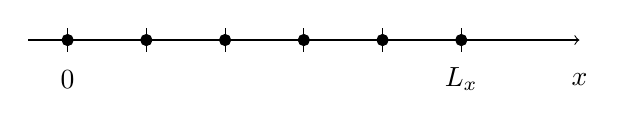
\begin{tikzpicture}
%\draw[fill=gray!23,gray!23](0,0) rectangle (8,2);
%\draw[step=0.5cm,gray,very thin] (0,0) grid (8,2); %background grid
\draw [->] (0.5,1) -- (7.5,1);
\draw[-] (1,0.85)--(1,1.15);
\draw[-] (2,0.85)--(2,1.15);
\draw[-] (3,0.85)--(3,1.15);
\draw[-] (4,0.85)--(4,1.15);
\draw[-] (5,0.85)--(5,1.15);
\draw[-] (6,0.85)--(6,1.15);
\node[] at (1,0.5) {$0$};
\node[] at (6,0.5) {$L_x$};
\node[] at (7.5,0.5) {$x$};
\draw[black,fill=black] (1,1)   circle (2pt);
\draw[black,fill=black] (2,1)   circle (2pt);
\draw[black,fill=black] (3,1)   circle (2pt);
\draw[black,fill=black] (4,1)   circle (2pt);
\draw[black,fill=black] (5,1)   circle (2pt);
\draw[black,fill=black] (6,1)   circle (2pt);
\end{tikzpicture}
\end{center}

\noindent
The distance between two consecutive coordinates is 
\[
h = \frac{L_x}{N-1}
\]
This simply translates as follows in Python:
\begin{lstlisting}
N=10
Lx=1
h=Lx/(N-1)
for i in range(0,N):
    print(i*h)
\end{lstlisting}

Since $i$ ranges from 0 to $N-1$ (because ... python!) the generated values go from 0 to $L_x$. 
Obviously I am doing this because I later wish to reuse these coordinates 
so I also wish to store them in an array.
I therefore need to declare and array of size $N$ which will 
contain all $N$ coordinates:
\begin{lstlisting}
import numpy as np
N=10
Lx=1
h=Lx/(N-1)
x=np.zeros(NV,dtype=np.float64)
for i in range(0,N):
    x[i]=i*h
\end{lstlisting}

What if now I wished the $N$ nodes (i.e. the coordinates of all points) to be placed between two arbitrary coordinates $x_{min}$ and $x_{max}$?

\begin{center}
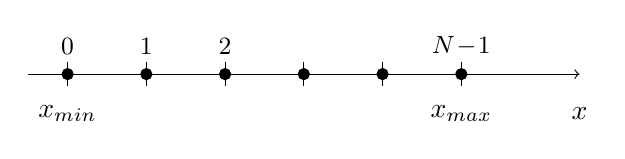
\begin{tikzpicture}
%\draw[fill=gray!23,gray!23](0,0) rectangle (8,2);
%\draw[step=0.5cm,gray,very thin] (0,0) grid (8,2); %background grid
\draw [->] (0.5,1) -- (7.5,1);
\draw[-] (1,0.85)--(1,1.15);
\draw[-] (2,0.85)--(2,1.15);
\draw[-] (3,0.85)--(3,1.15);
\draw[-] (4,0.85)--(4,1.15);
\draw[-] (5,0.85)--(5,1.15);
\draw[-] (6,0.85)--(6,1.15);
\node[] at (1,0.5) {$x_{min}$};
\node[] at (6,0.5) {$x_{max}$};
\node[] at (7.5,0.5) {$x$};
\draw[black,fill=black] (1,1)   circle (2pt);
\draw[black,fill=black] (2,1)   circle (2pt);
\draw[black,fill=black] (3,1)   circle (2pt);
\draw[black,fill=black] (4,1)   circle (2pt);
\draw[black,fill=black] (5,1)   circle (2pt);
\draw[black,fill=black] (6,1)   circle (2pt);
\node[] at (1,1.35) {\small 0};
\node[] at (2,1.35) {\small 1};
\node[] at (3,1.35) {\small 2};
\node[] at (6,1.35) {\small $N\!-\!1$};
\end{tikzpicture}
\end{center}

\noindent In this case the length of the domain is $L_x=x_{max}-x_{min}$, and the above code becomes:
\begin{lstlisting}
import numpy as np
N=10
xmin=-4
xmax=3
h=(xmax-xmin)/(N-1)
x=np.zeros(N,dtype=np.float64)
for i in range(0,N):
    x[i]=xmin+i*h
\end{lstlisting}
Note the presence of $x_{min}$ in the last line! 

\vspace{.8cm}

Unfortunately the world is definitely not one-dimensional, so 
I may want to build a two-dimensional grid spanning the domain 
$[0,L_x]\times[0,L_y]$ as depicted here:



\begin{center}
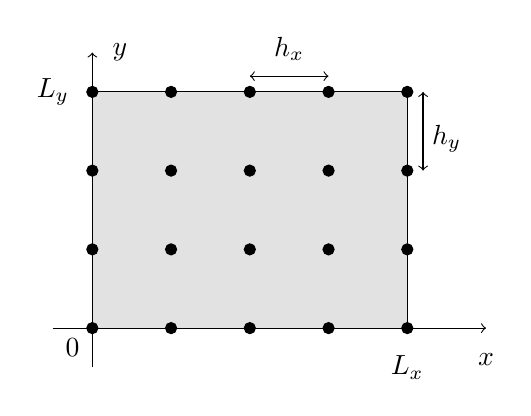
\begin{tikzpicture}
\draw[fill=gray!23,gray!23](1,1) rectangle (5,4);
%\draw[step=0.5cm,gray,very thin] (0,0) grid (7,5); 
\draw [->] (0.5,1) -- (6,1);
\draw [->] (1,0.5) -- (1,4.5);
\node[] at (0.75,0.75) {$0$};
\node[] at (5,0.5) {$L_x$};
\node[] at (0.5,4) {$L_y$};
\node[] at (6,0.6) {$x$};
\node[] at (1.35,4.5) {$y$};
\draw[-] (1,1)--(5,1)--(5,4)--(1,4)--cycle;
\draw[black,fill=black] (1,1)   circle (2pt);
\draw[black,fill=black] (2,1)   circle (2pt);
\draw[black,fill=black] (3,1)   circle (2pt);
\draw[black,fill=black] (4,1)   circle (2pt);
\draw[black,fill=black] (5,1)   circle (2pt);
\draw[black,fill=black] (1,2)   circle (2pt);
\draw[black,fill=black] (2,2)   circle (2pt);
\draw[black,fill=black] (3,2)   circle (2pt);
\draw[black,fill=black] (4,2)   circle (2pt);
\draw[black,fill=black] (5,2)   circle (2pt);
\draw[black,fill=black] (1,3)   circle (2pt);
\draw[black,fill=black] (2,3)   circle (2pt);
\draw[black,fill=black] (3,3)   circle (2pt);
\draw[black,fill=black] (4,3)   circle (2pt);
\draw[black,fill=black] (5,3)   circle (2pt);
\draw[black,fill=black] (1,4)   circle (2pt);
\draw[black,fill=black] (2,4)   circle (2pt);
\draw[black,fill=black] (3,4)   circle (2pt);
\draw[black,fill=black] (4,4)   circle (2pt);
\draw[black,fill=black] (5,4)   circle (2pt);
\draw[<->] (5.2,3)--(5.2,4);
\draw[<->] (3,4.2)--(4,4.2);
\node[] at (3.5,4.55) {$h_x$};
\node[] at (5.5,3.4) {$h_y$};
\end{tikzpicture}
\end{center}

\noindent There are now $N=N_x \times N_y$ nodes in the mesh, 
and we need to define the mesh spacing in both the $x$ and $y$
direction:
\[
h_x = \frac{L_x}{N_x-1}
\qquad\qquad
h_y = \frac{L_y}{N_y-1}
\]
From our experience with the 1D case, it seems logical to 
resort to a double for loop, one in the $x$ direction, 
one in the $y$ direction. 
However we must now make a decision as to which loop is inside the other (inner loop vs. outer loop). In essence, I must decide between 
\begin{lstlisting}
#approach 1
for i in range(0,Nx):
    for j in range(0,Ny):
\end{lstlisting}
and
\begin{lstlisting}
#approach 2
for j in range(0,Ny):
    for i in range(0,Nx):
\end{lstlisting}
As it turns out, I need not decide, both options are equally valid as we will see.
I now fix $N_x=4$ and $N_y=3$ so that the mesh contains 12 nodes:

\begin{center}
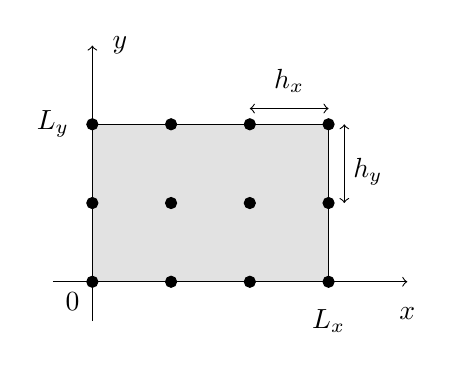
\begin{tikzpicture}
\draw[fill=gray!23,gray!23](1,1) rectangle (4,3);
%\draw[step=0.5cm,gray,very thin] (0,0) grid (7,5); 
\draw [->] (0.5,1) -- (5,1);
\draw [->] (1,0.5) -- (1,4);
\node[] at (0.75,0.75) {$0$};
\node[] at (4,0.5) {$L_x$};
\node[] at (0.5,3) {$L_y$};
\node[] at (5,0.6) {$x$};
\node[] at (1.35,4) {$y$};
\draw[-] (1,1)--(4,1)--(4,3)--(1,3)--cycle;
\draw[black,fill=black] (1,1)   circle (2pt);
\draw[black,fill=black] (2,1)   circle (2pt);
\draw[black,fill=black] (3,1)   circle (2pt);
\draw[black,fill=black] (4,1)   circle (2pt);
\draw[black,fill=black] (1,2)   circle (2pt);
\draw[black,fill=black] (2,2)   circle (2pt);
\draw[black,fill=black] (3,2)   circle (2pt);
\draw[black,fill=black] (4,2)   circle (2pt);
\draw[black,fill=black] (1,3)   circle (2pt);
\draw[black,fill=black] (2,3)   circle (2pt);
\draw[black,fill=black] (3,3)   circle (2pt);
\draw[black,fill=black] (4,3)   circle (2pt);
\draw[<->] (4.2,2)--(4.2,3);
\draw[<->] (3,3.2)--(4,3.2);
\node[] at (3.5,3.55) {$h_x$};
\node[] at (4.5,2.4) {$h_y$};
\end{tikzpicture}
\end{center}

\noindent Looking at approach \#1, I can include a print statement inside the loops as follows:
\begin{lstlisting}
#option 1
Nx=4
Ny=3
for i in range(0,Nx):
    for j in range(0,Ny):
        print('i=',i,'; j=',j)
\end{lstlisting}
If I was to run this code it would display (I first exhaust the $j$ values from the inner most loop before I switch to a different $i$ value):
\begin{lstlisting}
i= 0  ; j= 0
i= 0  ; j= 1
i= 0  ; j= 2
i= 1  ; j= 0
i= 1  ; j= 1
i= 1  ; j= 2
i= 2  ; j= 0
i= 2  ; j= 1
i= 2  ; j= 2
i= 3  ; j= 0
i= 3  ; j= 1
i= 3  ; j= 2
\end{lstlisting}
This means that the code is going through the nodes in the following order:
\begin{center}
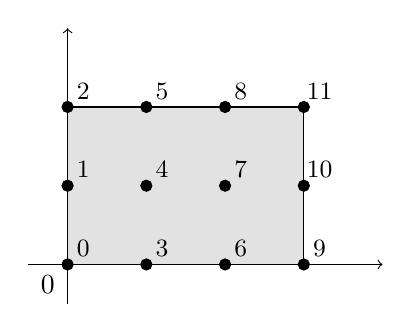
\begin{tikzpicture}
\draw[fill=gray!23,gray!23](1,1) rectangle (4,3);
%\draw[step=0.5cm,gray,very thin] (0,0) grid (7,5); 
\draw [->] (0.5,1) -- (5,1);
\draw [->] (1,0.5) -- (1,4);
\node[] at (0.75,0.75) {$0$};
\draw[-] (1,1)--(4,1)--(4,3)--(1,3)--cycle;
\draw[black,fill=black] (1,1)   circle (2pt);
\draw[black,fill=black] (2,1)   circle (2pt);
\draw[black,fill=black] (3,1)   circle (2pt);
\draw[black,fill=black] (4,1)   circle (2pt);
\draw[black,fill=black] (1,2)   circle (2pt);
\draw[black,fill=black] (2,2)   circle (2pt);
\draw[black,fill=black] (3,2)   circle (2pt);
\draw[black,fill=black] (4,2)   circle (2pt);
\draw[black,fill=black] (1,3)   circle (2pt);
\draw[black,fill=black] (2,3)   circle (2pt);
\draw[black,fill=black] (3,3)   circle (2pt);
\draw[black,fill=black] (4,3)   circle (2pt);
\node[] at (1.2,1.2) {\small $0$};
\node[] at (2.2,1.2) {\small $3$};
\node[] at (3.2,1.2) {\small $6$};
\node[] at (4.2,1.2) {\small $9$};
\node[] at (1.2,2.2) {\small $1$};
\node[] at (2.2,2.2) {\small $4$};
\node[] at (3.2,2.2) {\small $7$};
\node[] at (4.2,2.2) {\small $10$};
\node[] at (1.2,3.2) {\small $2$};
\node[] at (2.2,3.2) {\small $5$};
\node[] at (3.2,3.2) {\small $8$};
\node[] at (4.2,3.2) {\small $11$};
\end{tikzpicture}
\end{center}



Turning now to approach \#2, the same print statement will now yield:
\begin{lstlisting}
i= 0 ; j= 0
i= 1 ; j= 0
i= 2 ; j= 0
i= 3 ; j= 0
i= 0 ; j= 1
i= 1 ; j= 1
i= 2 ; j= 1
i= 3 ; j= 1
i= 0 ; j= 2
i= 1 ; j= 2
i= 2 ; j= 2
i= 3 ; j= 2
\end{lstlisting}
and this corresponds then to the following order: 
\begin{center}
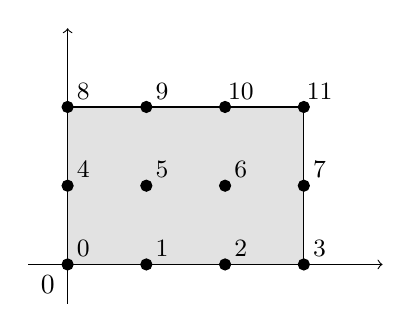
\begin{tikzpicture}
\draw[fill=gray!23,gray!23](1,1) rectangle (4,3);
%\draw[step=0.5cm,gray,very thin] (0,0) grid (7,5); 
\draw [->] (0.5,1) -- (5,1);
\draw [->] (1,0.5) -- (1,4);
\node[] at (0.75,0.75) {$0$};
\draw[-] (1,1)--(4,1)--(4,3)--(1,3)--cycle;
\draw[black,fill=black] (1,1)   circle (2pt);
\draw[black,fill=black] (2,1)   circle (2pt);
\draw[black,fill=black] (3,1)   circle (2pt);
\draw[black,fill=black] (4,1)   circle (2pt);
\draw[black,fill=black] (1,2)   circle (2pt);
\draw[black,fill=black] (2,2)   circle (2pt);
\draw[black,fill=black] (3,2)   circle (2pt);
\draw[black,fill=black] (4,2)   circle (2pt);
\draw[black,fill=black] (1,3)   circle (2pt);
\draw[black,fill=black] (2,3)   circle (2pt);
\draw[black,fill=black] (3,3)   circle (2pt);
\draw[black,fill=black] (4,3)   circle (2pt);
\node[] at (1.2,1.2) {\small $0$};
\node[] at (2.2,1.2) {\small $1$};
\node[] at (3.2,1.2) {\small $2$};
\node[] at (4.2,1.2) {\small $3$};
\node[] at (1.2,2.2) {\small $4$};
\node[] at (2.2,2.2) {\small $5$};
\node[] at (3.2,2.2) {\small $6$};
\node[] at (4.2,2.2) {\small $7$};
\node[] at (1.2,3.2) {\small $8$};
\node[] at (2.2,3.2) {\small $9$};
\node[] at (3.2,3.2) {\small $10$};
\node[] at (4.2,3.2) {\small $11$};
\end{tikzpicture}
\end{center}

\noindent In the end, we see that both approaches yield a valid 
numbering scheme, one is 'lines first' , the other 'columns first'.

In what follows I focus on approach \#2, only because it seems more 'natural' to me than the other one (it goes from left to right, then bottom to top). 
Our proto-code then looks like this:
\begin{lstlisting}
Lx=10
Ly=8
Nx=4
Ny=3
N=Nx*Ny
hx=Lx/(Nx-1)
hy=Ly/(Ny-1)
x=np.zeros(N,dtype=np.float64)
y=np.zeros(N,dtype=np.float64)
for j in range(0,Ny):
    for i in range(0,Nx):
        x[?]=i*hx
        y[?]=j*hy
\end{lstlisting}
Note that I have left two question marks. One may want to replace these by $i$ and $j$, 
following our experience in the 1D case. However, remember that $i$ ($j$) ranges between 
$0$ and $N_x-1=3$ ($0$ and $N_y-1=2$ respectively) but we need to assign and store the 
coordinates of all 12 nodes. 

So what should I write instead of question marks? Effectively, I need some form of counter 
so that every time the inner loop is executed the counter is incremented by one. 
When all $i,j$ combinations are exhausted this counter should have reached the 
last node. Such a counter can be implemented as follows:
\begin{lstlisting}
counter=0
for j in range(0,Ny):
    for i in range(0,Nx):
        print('counter=',counter,'i=',i,'; j=',j,j*Nx+i)
        counter+=1
\end{lstlisting}
It must be initialised to zero, and it is incremented $N_x \cdot N_y$ times.
Running this code would yield 
\begin{lstlisting}
counter=  0 i= 0 ; j= 0
counter=  1 i= 1 ; j= 0
counter=  2 i= 2 ; j= 0
counter=  3 i= 3 ; j= 0
counter=  4 i= 0 ; j= 1
counter=  5 i= 1 ; j= 1
counter=  6 i= 2 ; j= 1
counter=  7 i= 3 ; j= 1
counter=  8 i= 0 ; j= 2
counter=  9 i= 1 ; j= 2
counter= 10 i= 2 ; j= 2
counter= 11 i= 3 ; j= 2
\end{lstlisting}
We see that the counter takes all 12 values between 0 and 11, so it is the index I am looking for. Finally, the 2D code (or approach \#2) looks like:
\begin{lstlisting}
Lx=10
Ly=8
Nx=4
Ny=3
N=Nx*Ny
hx=Lx/(Nx-1)
hy=Ly/(Ny-1)
x=np.zeros(N,dtype=np.float64)
y=np.zeros(N,dtype=np.float64)
counter=0
for j in range(0,Ny):
    for i in range(0,Nx):
        x[counter]=i*hx
        y[counter]=j*hy
        counter+=1
\end{lstlisting}
It is trivial to verify that one can swap the two lines with the 'for' statements to obtain the approach \#1 version of the code.

Before I move to the three-dimensional case, I wish to mention a slightly different 
approach than the 'counter' one. 
Looking back at the numbering generated by approach \#2, it is easy to see that the node number (i.e. a value between 0 and 11)
can be also computed with $j\cdot N_x+i$. You can indeed verify that this expression yields the same values as the counter here above for all the $i,j$ combinations. However one must realise that this formula is not valid for approach \#1. The code then becomes:
\begin{lstlisting}
Lx=10
Ly=8
Nx=4
Ny=3
N=Nx*Ny
hx=Lx/(Nx-1)
hy=Ly/(Ny-1)
x=np.zeros(N,dtype=np.float64)
y=np.zeros(N,dtype=np.float64)
for j in range(0,Ny):
    for i in range(0,Nx):
        x[j*Nx+i]=i*hx
        y[j*Nx+i]=j*hy
\end{lstlisting}

Also, if the domain is not $[0,L_x]\times[0,L_y]$ but
$[x_{min},x_{max}]\times[y_{min},y_{max}]$, the code becomes
\begin{lstlisting}
xmin=-3
xmax=5
ymin=-1
ymax=4
Nx=4
Ny=3
N=Nx*Ny
hx=(xmax-xmin)/(Nx-1)
hy=(ymax-ymin)/(Ny-1)
x=np.zeros(N,dtype=np.float64)
y=np.zeros(N,dtype=np.float64)
for j in range(0,Ny):
    for i in range(0,Nx):
        x[j*Nx+i]=xmin+i*hx
        y[j*Nx+i]=ymin+j*hy
\end{lstlisting}

\vspace{.8cm}

Extending the codes above to three-dimensions is rather trivial, especially when the counter approach 
is used. One must simply be aware of the order of the loops (there are 3\! =6 approaches).
\begin{lstlisting}
xmin=-3
xmax=5
ymin=-1
ymax=4
zmin=1
zmax=6
Nx=4
Ny=3
Nz=5
N=Nx*Ny*Nz
hx=(xmax-xmin)/(Nx-1)
hy=(ymax-ymin)/(Ny-1)
hz=(zmax-zmin)/(Nz-1)
x=np.zeros(N,dtype=np.float64)
y=np.zeros(N,dtype=np.float64)
z=np.zeros(N,dtype=np.float64)
counter
for k in range(0,Nz):
    for j in range(0,Ny):
        for i in range(0,Nx):
            x[counter]=xmin+i*hx
            y[counter]=ymin+j*hy
            z[counter]=zmin+j*hz
            counter+=1
\end{lstlisting}
You will find near identical codes in (for example) Stone 1 and 10.

\vspace{.8cm}

In some cases, we wish to store the coordinates of the mesh nodes because the nodes 
make a regular grid of quadrilaterals on which ODEs or PDEs will be solved:

\begin{center}
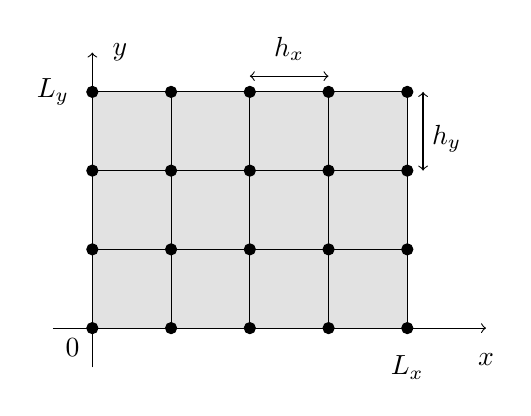
\begin{tikzpicture}
\draw[fill=gray!23,gray!23](1,1) rectangle (5,4);
%\draw[step=0.5cm,gray,very thin] (0,0) grid (7,5); 
\draw [->] (0.5,1) -- (6,1);
\draw [->] (1,0.5) -- (1,4.5);
\node[] at (0.75,0.75) {$0$};
\node[] at (5,0.5) {$L_x$};
\node[] at (0.5,4) {$L_y$};
\node[] at (6,0.6) {$x$};
\node[] at (1.35,4.5) {$y$};
\draw[-] (1,1)--(5,1)--(5,4)--(1,4)--cycle;
\draw[-] (1,2)--(5,2);
\draw[-] (1,3)--(5,3);
\draw[-] (2,1)--(2,4);
\draw[-] (3,1)--(3,4);
\draw[-] (4,1)--(4,4);
\draw[black,fill=black] (1,1)   circle (2pt);
\draw[black,fill=black] (2,1)   circle (2pt);
\draw[black,fill=black] (3,1)   circle (2pt);
\draw[black,fill=black] (4,1)   circle (2pt);
\draw[black,fill=black] (5,1)   circle (2pt);
\draw[black,fill=black] (1,2)   circle (2pt);
\draw[black,fill=black] (2,2)   circle (2pt);
\draw[black,fill=black] (3,2)   circle (2pt);
\draw[black,fill=black] (4,2)   circle (2pt);
\draw[black,fill=black] (5,2)   circle (2pt);
\draw[black,fill=black] (1,3)   circle (2pt);
\draw[black,fill=black] (2,3)   circle (2pt);
\draw[black,fill=black] (3,3)   circle (2pt);
\draw[black,fill=black] (4,3)   circle (2pt);
\draw[black,fill=black] (5,3)   circle (2pt);
\draw[black,fill=black] (1,4)   circle (2pt);
\draw[black,fill=black] (2,4)   circle (2pt);
\draw[black,fill=black] (3,4)   circle (2pt);
\draw[black,fill=black] (4,4)   circle (2pt);
\draw[black,fill=black] (5,4)   circle (2pt);
\draw[<->] (5.2,3)--(5.2,4);
\draw[<->] (3,4.2)--(4,4.2);
\node[] at (3.5,4.55) {$h_x$};
\node[] at (5.5,3.4) {$h_y$};
\end{tikzpicture}
\end{center}

There are $N_x$ nodes in the $x$ direction but only $N_x-1$ cells/elements\footnote{Because of my 
bias towards the Finite Element Method, I will refer to these as elements.}. 
Likewise there are $N_y$ nodes in the $y$ direction but only $N_y-1$ cells/elements.
In total there are $N_e=(N_x-1)(N_y-1)$ elements. 
As for the cell center nodes, we must adopt a systematic way of numbering them. 
If I keep using approach \#2 for the nodes, the following numbering of 
{\color{teal}elements} seems natural:

\begin{center}
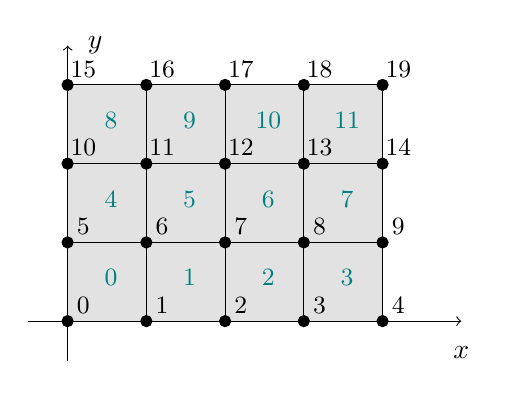
\begin{tikzpicture}
\draw[fill=gray!23,gray!23](1,1) rectangle (5,4);
%\draw[step=0.5cm,gray,very thin] (0,0) grid (7,5); 
\draw [->] (0.5,1) -- (6,1);
\draw [->] (1,0.5) -- (1,4.5);
\node[] at (6,0.6) {$x$};
\node[] at (1.35,4.5) {$y$};
\draw[-] (1,1)--(5,1)--(5,4)--(1,4)--cycle;
\draw[-] (1,2)--(5,2);
\draw[-] (1,3)--(5,3);
\draw[-] (2,1)--(2,4);
\draw[-] (3,1)--(3,4);
\draw[-] (4,1)--(4,4);
\draw[black,fill=black] (1,1)   circle (2pt);
\draw[black,fill=black] (2,1)   circle (2pt);
\draw[black,fill=black] (3,1)   circle (2pt);
\draw[black,fill=black] (4,1)   circle (2pt);
\draw[black,fill=black] (5,1)   circle (2pt);
\draw[black,fill=black] (1,2)   circle (2pt);
\draw[black,fill=black] (2,2)   circle (2pt);
\draw[black,fill=black] (3,2)   circle (2pt);
\draw[black,fill=black] (4,2)   circle (2pt);
\draw[black,fill=black] (5,2)   circle (2pt);
\draw[black,fill=black] (1,3)   circle (2pt);
\draw[black,fill=black] (2,3)   circle (2pt);
\draw[black,fill=black] (3,3)   circle (2pt);
\draw[black,fill=black] (4,3)   circle (2pt);
\draw[black,fill=black] (5,3)   circle (2pt);
\draw[black,fill=black] (1,4)   circle (2pt);
\draw[black,fill=black] (2,4)   circle (2pt);
\draw[black,fill=black] (3,4)   circle (2pt);
\draw[black,fill=black] (4,4)   circle (2pt);
\draw[black,fill=black] (5,4)   circle (2pt);
\node[] at (1.2,1.2) {\small $0$};
\node[] at (2.2,1.2) {\small $1$};
\node[] at (3.2,1.2) {\small $2$};
\node[] at (4.2,1.2) {\small $3$};
\node[] at (5.2,1.2) {\small $4$};
\node[] at (1.2,2.2) {\small $5$};
\node[] at (2.2,2.2) {\small $6$};
\node[] at (3.2,2.2) {\small $7$};
\node[] at (4.2,2.2) {\small $8$};
\node[] at (5.2,2.2) {\small $9$};
\node[] at (1.2,3.2) {\small $10$};
\node[] at (2.2,3.2) {\small $11$};
\node[] at (3.2,3.2) {\small $12$};
\node[] at (4.2,3.2) {\small $13$};
\node[] at (5.2,3.2) {\small $14$};
\node[] at (1.2,4.2) {\small $15$};
\node[] at (2.2,4.2) {\small $16$};
\node[] at (3.2,4.2) {\small $17$};
\node[] at (4.2,4.2) {\small $18$};
\node[] at (5.2,4.2) {\small $19$};
\node[] at (1.55,1.55) {\color{teal} \small $0$};
\node[] at (2.55,1.55) {\color{teal} \small $1$};
\node[] at (3.55,1.55) {\color{teal} \small $2$};
\node[] at (4.55,1.55) {\color{teal} \small $3$};
\node[] at (1.55,2.55) {\color{teal} \small $4$};
\node[] at (2.55,2.55) {\color{teal} \small $5$};
\node[] at (3.55,2.55) {\color{teal} \small $6$};
\node[] at (4.55,2.55) {\color{teal} \small $7$};
\node[] at (1.55,3.55) {\color{teal} \small $8$};
\node[] at (2.55,3.55) {\color{teal} \small $9$};
\node[] at (3.55,3.55) {\color{teal} \small $10$};
\node[] at (4.55,3.55) {\color{teal} \small $11$};
\end{tikzpicture}
\end{center}

In some applications we want to also store the coordinates of the center of all cells, i.e. the $N_e$ coordinates of {\color{teal} these} points:

\begin{center}
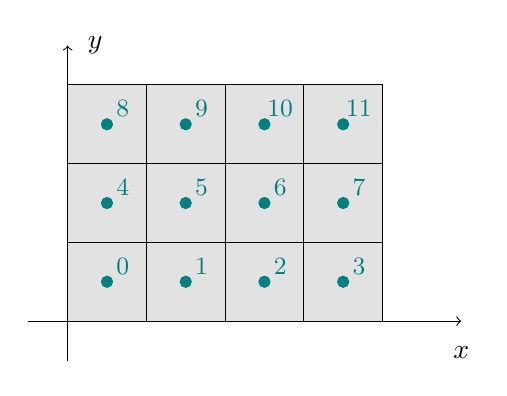
\begin{tikzpicture}
\draw[fill=gray!23,gray!23](1,1) rectangle (5,4);
%\draw[step=0.5cm,gray,very thin] (0,0) grid (7,5); 
\draw [->] (0.5,1) -- (6,1);
\draw [->] (1,0.5) -- (1,4.5);
\node[] at (6,0.6) {$x$};
\node[] at (1.35,4.5) {$y$};
\draw[-] (1,1)--(5,1)--(5,4)--(1,4)--cycle;
\draw[-] (1,2)--(5,2);
\draw[-] (1,3)--(5,3);
\draw[-] (2,1)--(2,4);
\draw[-] (3,1)--(3,4);
\draw[-] (4,1)--(4,4);
\draw[black,fill=black,color=teal] (1.5,1.5)   circle (2pt);
\draw[black,fill=black,color=teal] (2.5,1.5)   circle (2pt);
\draw[black,fill=black,color=teal] (3.5,1.5)   circle (2pt);
\draw[black,fill=black,color=teal] (4.5,1.5)   circle (2pt);
\draw[black,fill=black,color=teal] (1.5,2.5)   circle (2pt);
\draw[black,fill=black,color=teal] (2.5,2.5)   circle (2pt);
\draw[black,fill=black,color=teal] (3.5,2.5)   circle (2pt);
\draw[black,fill=black,color=teal] (4.5,2.5)   circle (2pt);
\draw[black,fill=black,color=teal] (1.5,3.5)   circle (2pt);
\draw[black,fill=black,color=teal] (2.5,3.5)   circle (2pt);
\draw[black,fill=black,color=teal] (3.5,3.5)   circle (2pt);
\draw[black,fill=black,color=teal] (4.5,3.5)   circle (2pt);
\node[] at (1.7,1.7) {\color{teal} \small $0$};
\node[] at (2.7,1.7) {\color{teal} \small $1$};
\node[] at (3.7,1.7) {\color{teal} \small $2$};
\node[] at (4.7,1.7) {\color{teal} \small $3$};
\node[] at (1.7,2.7) {\color{teal} \small $4$};
\node[] at (2.7,2.7) {\color{teal} \small $5$};
\node[] at (3.7,2.7) {\color{teal} \small $6$};
\node[] at (4.7,2.7) {\color{teal} \small $7$};
\node[] at (1.7,3.7) {\color{teal} \small $8$};
\node[] at (2.7,3.7) {\color{teal} \small $9$};
\node[] at (3.7,3.7) {\color{teal} \small $10$};
\node[] at (4.7,3.7) {\color{teal} \small $11$};
\end{tikzpicture}
\end{center}
Given this numbering these points form a regular grid:
\begin{center}
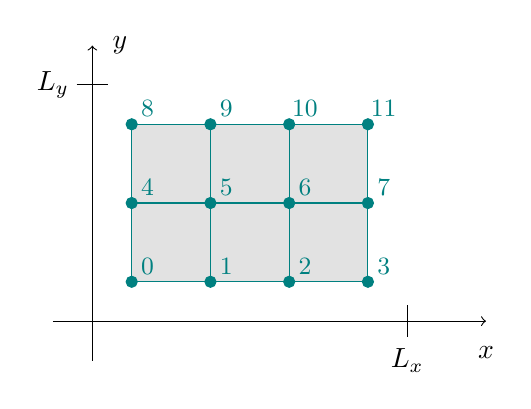
\begin{tikzpicture}
\draw[fill=gray!23,gray!23](1.5,1.5) rectangle (4.5,3.5);
%\draw[step=0.5cm,gray,very thin] (0,0) grid (7,5); 
\draw [->] (0.5,1) -- (6,1);
\draw [->] (1,0.5) -- (1,4.5);
\node[] at (6,0.6) {$x$};
\node[] at (1.35,4.5) {$y$};
\draw[-,teal] (1.5,1.5)--(4.5,1.5)--(4.5,3.5)--(1.5,3.5)--cycle;
\draw[-,teal] (1.5,2.5)--(4.5,2.5);
\draw[-,teal] (2.5,1.5)--(2.5,3.5);
\draw[-,teal] (3.5,1.5)--(3.5,3.5);
\draw[black,fill=black,color=teal] (1.5,1.5)   circle (2pt);
\draw[black,fill=black,color=teal] (2.5,1.5)   circle (2pt);
\draw[black,fill=black,color=teal] (3.5,1.5)   circle (2pt);
\draw[black,fill=black,color=teal] (4.5,1.5)   circle (2pt);
\draw[black,fill=black,color=teal] (1.5,2.5)   circle (2pt);
\draw[black,fill=black,color=teal] (2.5,2.5)   circle (2pt);
\draw[black,fill=black,color=teal] (3.5,2.5)   circle (2pt);
\draw[black,fill=black,color=teal] (4.5,2.5)   circle (2pt);
\draw[black,fill=black,color=teal] (1.5,3.5)   circle (2pt);
\draw[black,fill=black,color=teal] (2.5,3.5)   circle (2pt);
\draw[black,fill=black,color=teal] (3.5,3.5)   circle (2pt);
\draw[black,fill=black,color=teal] (4.5,3.5)   circle (2pt);
\node[] at (1.7,1.7) {\color{teal} \small $0$};
\node[] at (2.7,1.7) {\color{teal} \small $1$};
\node[] at (3.7,1.7) {\color{teal} \small $2$};
\node[] at (4.7,1.7) {\color{teal} \small $3$};
\node[] at (1.7,2.7) {\color{teal} \small $4$};
\node[] at (2.7,2.7) {\color{teal} \small $5$};
\node[] at (3.7,2.7) {\color{teal} \small $6$};
\node[] at (4.7,2.7) {\color{teal} \small $7$};
\node[] at (1.7,3.7) {\color{teal} \small $8$};
\node[] at (2.7,3.7) {\color{teal} \small $9$};
\node[] at (3.7,3.7) {\color{teal} \small $10$};
\node[] at (4.7,3.7) {\color{teal} \small $11$};
\draw[-] (5,0.8)--(5,1.2);
\draw[-] (0.8,4)--(1.2,4);
\node[] at (5,0.5) {$L_x$};
\node[] at (0.5,4) {$L_y$};
\end{tikzpicture}
\end{center}
This 'new' domain is bound by $x'_{min}=h_x/2$, $x'_{max}=L_x-h_x/2$ in 
the $x$ direction and $y'_{min}=h/2$, $y'_{max}=L_y-h_y/2$ in the $y$ direction. We note that the spacings $h_x$ and $h_y$ between the centers is the same as for the nodes. 
We store the coordinates $(x_c,y_c)$ of the cell centers in two arrays of length $N_e$ and the code is then simply

\begin{lstlisting}
Lx=9
Ly=7
Nx=4
Ny=3
N=Nx*Ny
hx=(xmax-xmin)/(Nx-1)
hy=(ymax-ymin)/(Ny-1)
#mesh nodes coordinates
x=np.zeros(N,dtype=np.float64)
y=np.zeros(N,dtype=np.float64)
counter=0
for j in range(0,Ny):
    for i in range(0,Nx):
        x[counter]=i*hx
        y[counter]=j*hy
        counter+=1
#cell centers coordinates
Ne=(Nx-1)*(Ny-1)
xc=np.zeros(Ne,dtype=np.float64)
yc=np.zeros(Ne,dtype=np.float64)
xmin=hx/2
xmax=Lx-hx/2
ymin=hy/2
ymax=Ly-hy/2
counter=0
for j in range(0,Ny-1):
    for i in range(0,Nx-1):
        xc[counter]=xmin+i*hx
        yc[counter]=ymin+j*hy
        counter+=1
\end{lstlisting}





 %%%%%%%%%%%%%%%%%%%%%%%%%%%%%%%%%%%%%%%%%%%%%%%%%

\newpage %%%%%%%%%%%%%%%%%%%%%%%%%%%%%%%%%%%%%%%%%%%%%%%%%%%%%%%%%%%%%%%%%%%%%%%%%%%%%%%%
\section*{
Stone 01: simple analytical solution (D\&H) 
\label{f01}}
\addcontentsline{toc}{section}{\protect\numberline{} 
Stone 01: simple analytical solution (D\&H) 
}

From \cite{dohu}. In order to illustrate the behavior of selected mixed finite elements in the solution 
of stationary Stokes flow,  we consider a two-dimensional problem 
in the square domain $\Omega=[0,1]\times[0,1]$, which possesses a closed-form analytical 
solution. The problem consists of determining the velocity field ${\bm v} = (u,v)$ and the 
pressure $p$ such that 
\[
-\nu \Delta {\bm v} + {\bm \nabla} p = {\bm b}  \quad\quad {\rm in} \; \Omega
\]
\[
{\bm \nabla} \cdot {\bm v} = 0 \quad\quad {\rm in} \; \Omega
\]
\[
{\bm v}={\bm 0} \quad\quad {\rm on} \; \Gamma
\]
where the fluid viscosity is taken as $\nu=1$. The components of the body force ${\bm b}$ are prescribed as 
\begin{eqnarray}
b_x &=& (12 - 24y) x^4 + (-24 + 48y) x^3 + (-48y + 72y^2 - 48 y^3 + 12) x^2 \nonumber\\
    && + (-2 + 24y -72y^2+48y^3)x + 1-4y + 12y^2-8y^3 \nonumber\\ 
b_y &=& (8 - 48y + 48 y^2) x^3 + (-12 + 72y - 72y^2) x^2  \nonumber\\
    && + (4 - 24y + 48y^2 - 48y^3 + 24y^4) x - 12y^2 + 24y^3 - 12y^4  \nonumber
\end{eqnarray}
With this prescribed body force, the exact solution is 
\begin{eqnarray}
u(x,y) &=& x^2(1- x)^2 (2y - 6y^2 + 4y^3)  \nonumber\\
v(x,y) &=& -y^2 (1 - y)^2 (2x - 6x^2 + 4x^3) \nonumber\\
p(x,y) &=& x(1 -x)- 1/6 \nonumber 
\end{eqnarray}
Note that the pressure obeys $\int_{\Omega} p \; d\Omega = 0$

\fbox{
\parbox{10cm}{{\bf features}
\begin{itemize}
\item $Q_1\times P_0$ element \index{$Q_1 \times P_0$}
\item incompressible flow
\item penalty formulation \index{penalty formulation}
\item Dirichlet boundary conditions (no-slip)
\item direct solver 
\item isothermal \index{isothermal}
\item isoviscous \index{isoviscous}
\item analytical solution \index{analytical solution}
\end{itemize}
}}

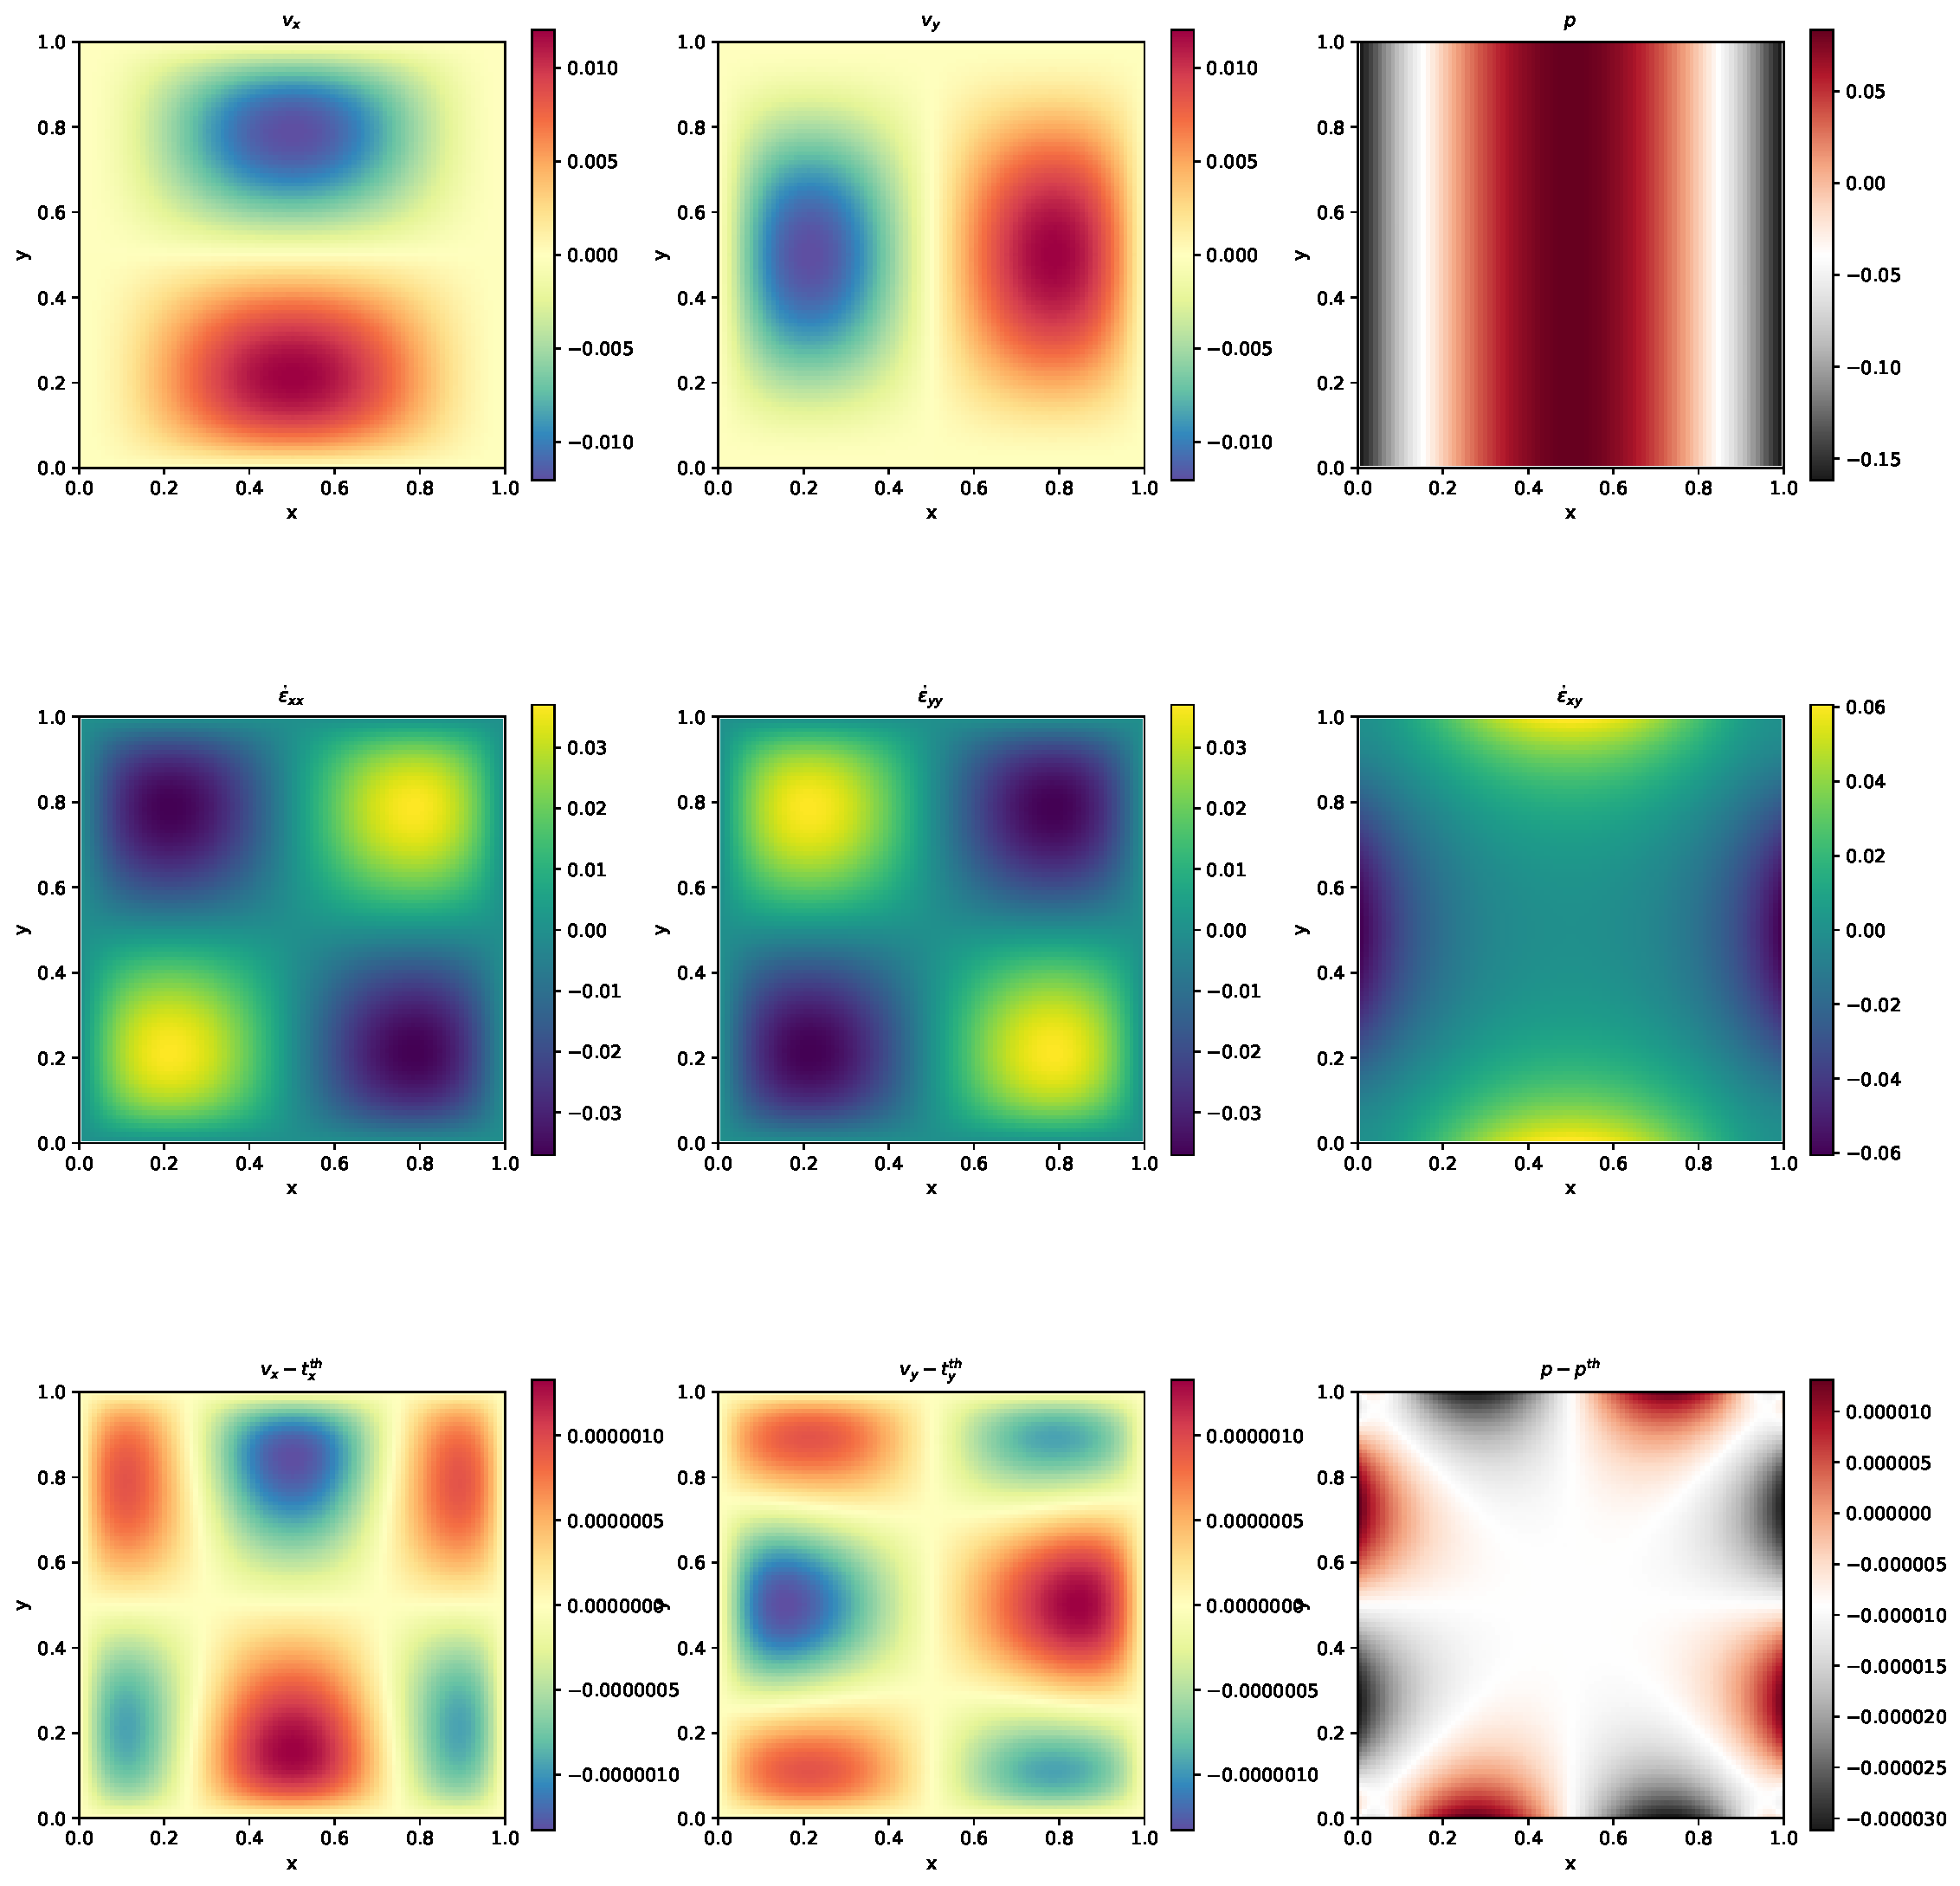
\includegraphics[width=16cm]{python_codes/fieldstone_01/solution.pdf}

\begin{center}
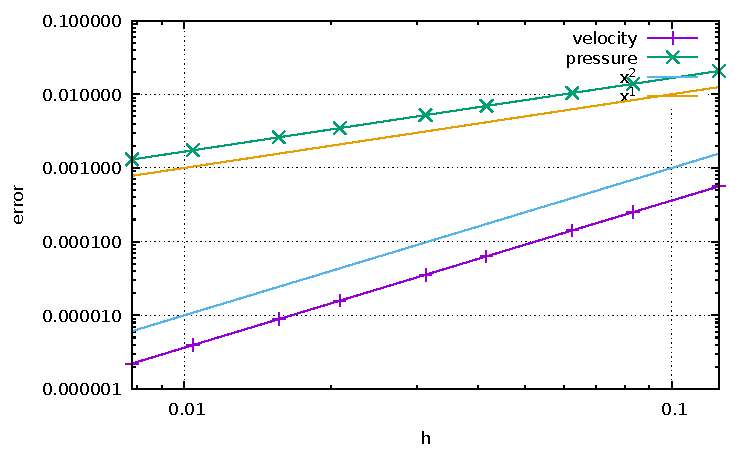
\includegraphics[width=12cm]{python_codes/fieldstone_01/errors.pdf}\\
Quadratic convergence for velocity error, 
linear convergence for pressure error, as expected.
\end{center}

ToDo:

pressure normalisation?

different cmat, a la schmalholz

To go further:
\begin{enumerate}
\item make your own analytical solution
\end{enumerate}
 %%%%%%%%%%%%%%%%%%%%%%%%%%%%%%%%%%%%%%%%%%%%%%%%%

\newpage %%%%%%%%%%%%%%%%%%%%%%%%%%%%%%%%%%%%%%%%%%%%%%%%%%%%%%%%%%%%%%%%%%%%%%%%%%%%%%%%
\section*{
Stone 02: Stokes sphere in 2D with $Q_1\times P_0$ elements \& penalty formulation 
\label{f02}}
\addcontentsline{toc}{section}{\protect\numberline{} 
Stone 02: Stokes sphere in 2D with $Q_1\times P_0$ elements \& penalty formulation 
}
\lstinputlisting[language=bash,basicstyle=\small]{python_codes/fieldstone_02/keywords}

\begin{center}
Code at \url{https://github.com/cedrict/fieldstone/tree/master/python_codes/fieldstone_02}
\end{center}

\par\noindent\rule{\textwidth}{0.4pt}
%%%%%%%%%%%%%%%%%%%%%%%%%%%%%%%%%%%%%%%%%%%%%%%%%%%%%%%%%%%%%%%%%%%%%%%%%%%%%%%%%%%%%%%%%

The domain is a unit square. The fluid is characterised 
by $\rho=1$ and $\eta=1$ 
while the sphere is characterised 
by $\rho=2$ and $\eta=1000$.
The gravity vector is $\vec{g}=(0,-1)$. 
Boundary conditions are free slip on all sides.
Viscosity and density directly computed at the quadrature points.

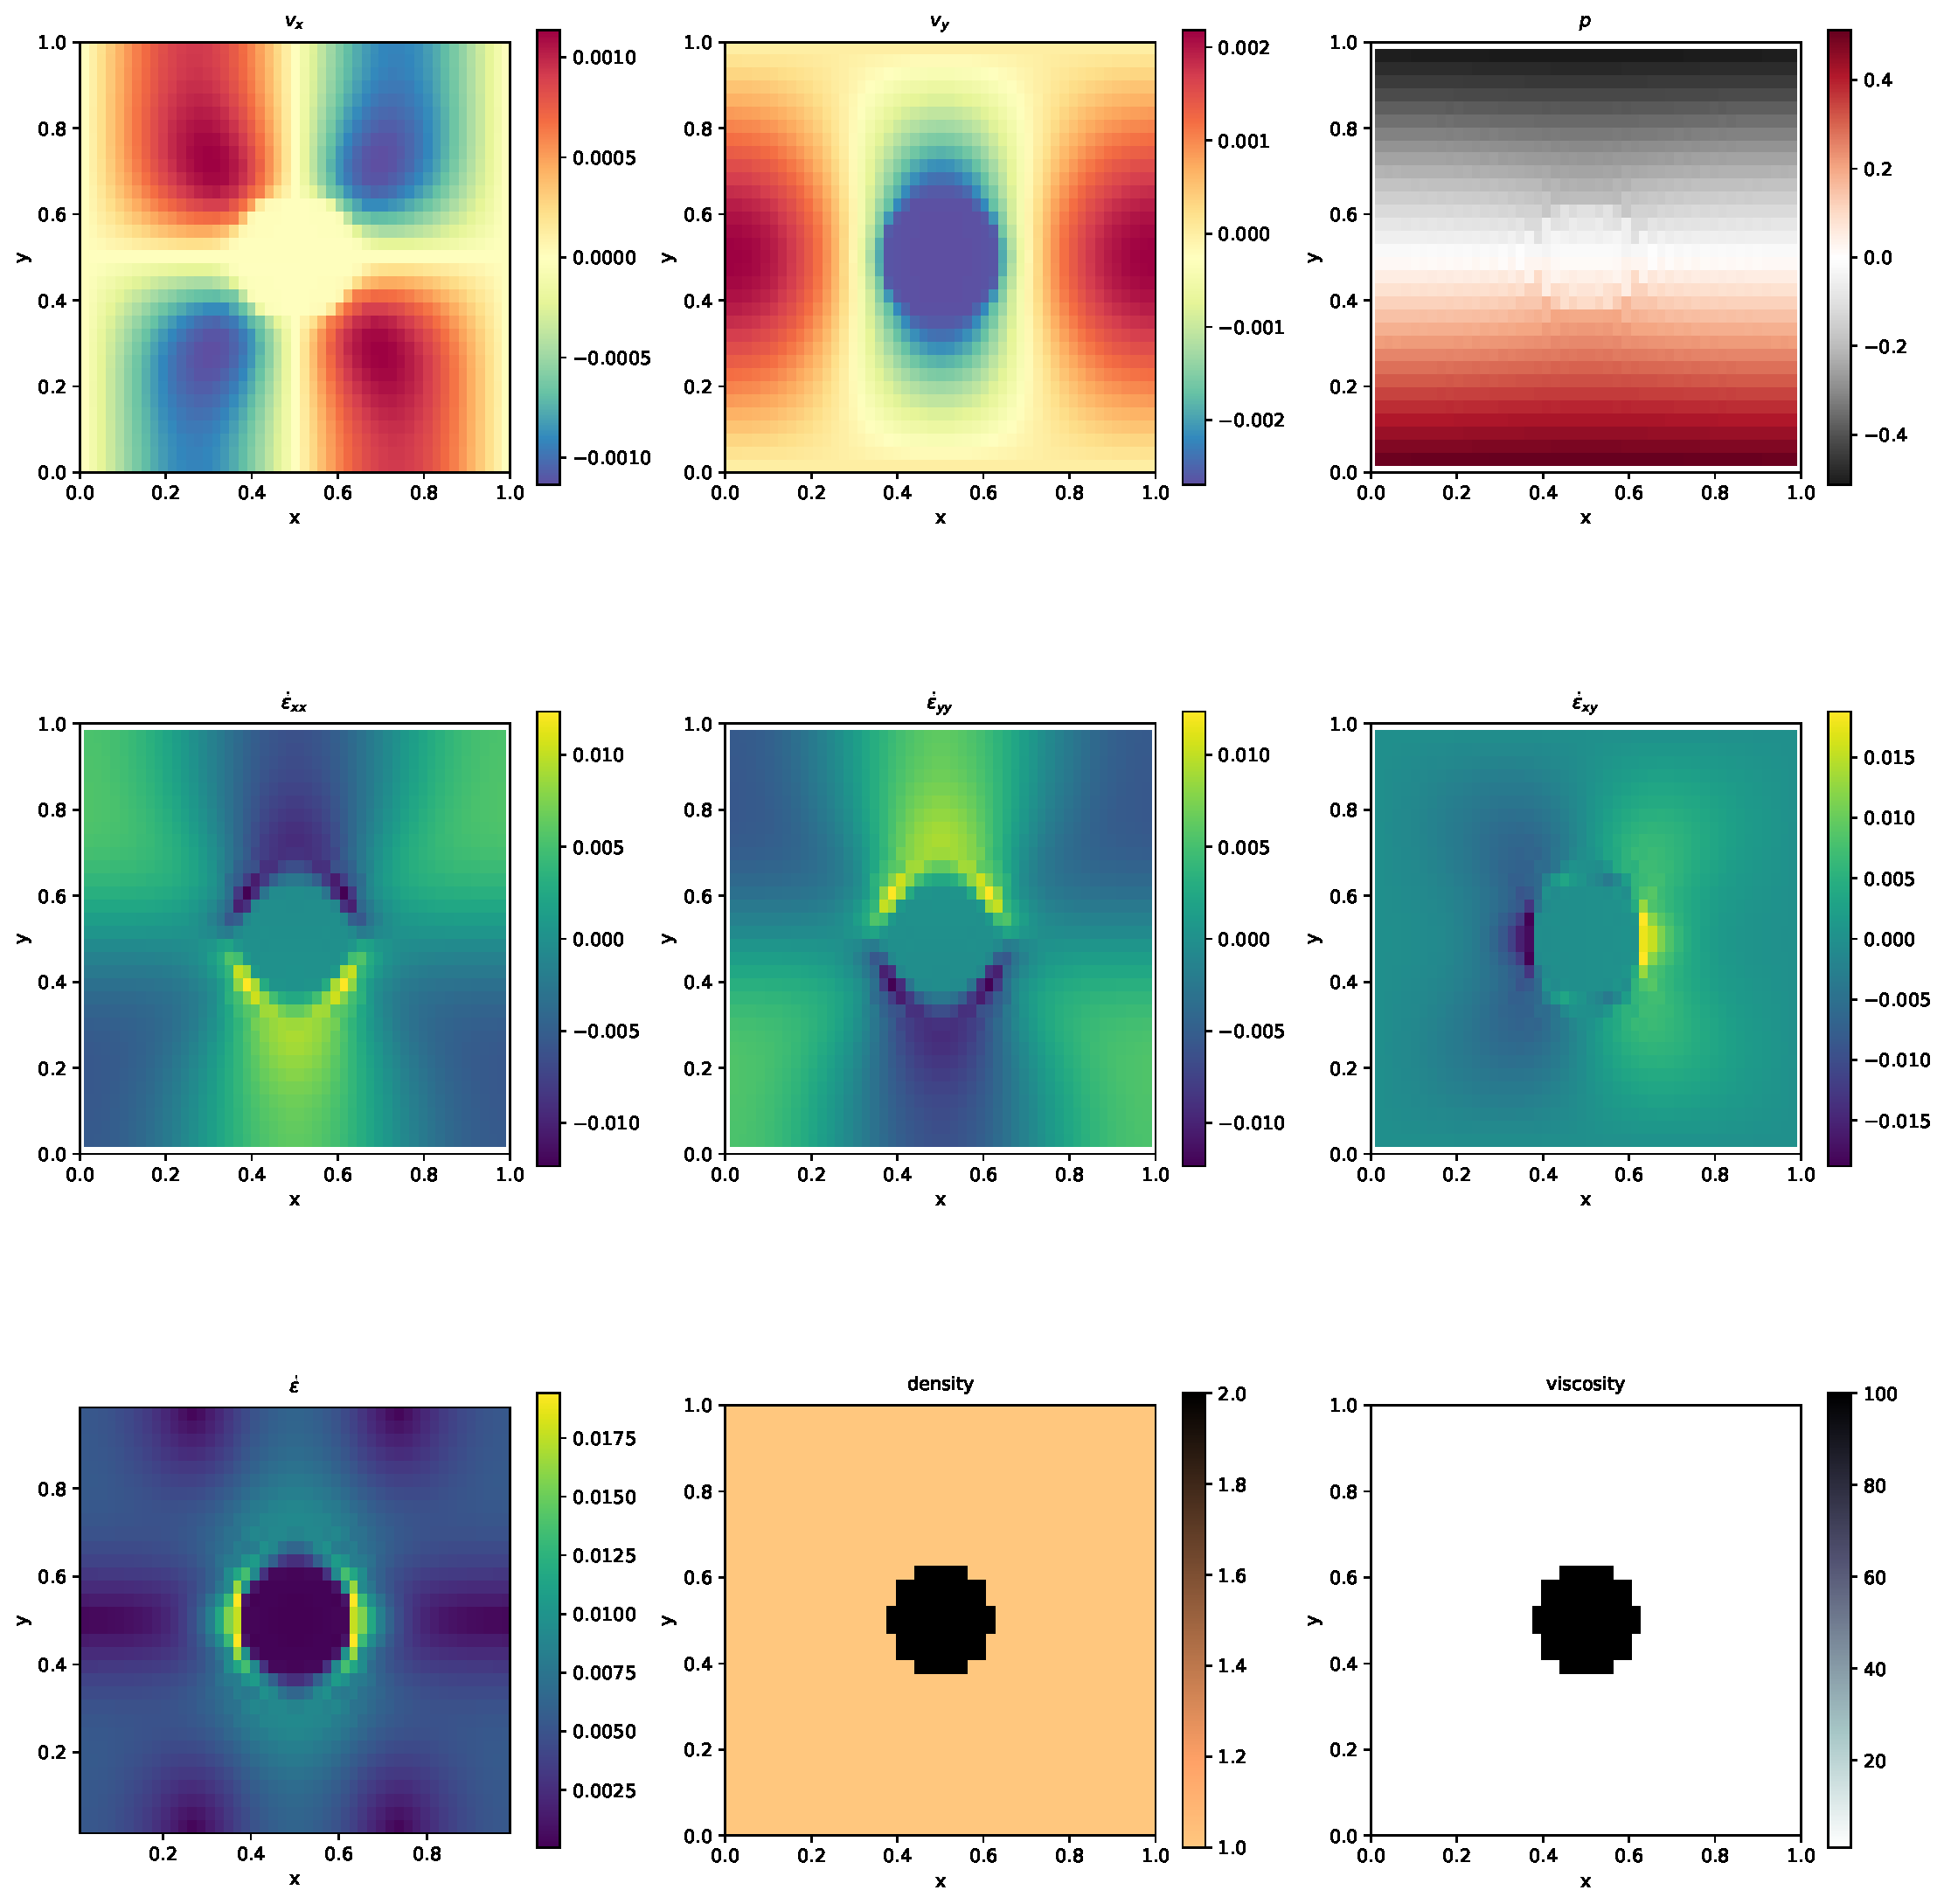
\includegraphics[width=15cm]{python_codes/fieldstone_02/solution.pdf}

 %%%%%%%%%%%%%%%%%%%%%%%%%%%%%%%%%%%%%%%%%%%%%%%%%

\newpage %%%%%%%%%%%%%%%%%%%%%%%%%%%%%%%%%%%%%%%%%%%%%%%%%%%%%%%%%%%%%%%%%%%%%%%%%%%%%%%%
\section*{
Stone 03: Convection in a 2D box 
\label{f03}}
\addcontentsline{toc}{section}{\protect\numberline{} 
Stone 03: Convection in a 2D box 
}

\lstinputlisting[language=bash,basicstyle=\small]{python_codes/fieldstone_03/keywords}

This benchmark deals with the 2-D thermal convection of a fluid 
of infinite Prandtl number in a rectangular closed cell.
In what follows, I carry out the case 1a, 1b, and 1c experiments as shown in \cite{blbc89}:
steady convection with constant viscosity in a square box.

The temperature is fixed to zero on top and to $\Delta T$ at the bottom, 
with reflecting symmetry at the sidewalls (i.e. $\partial_x T=0$) 
and there are no internal heat sources. 
Free-slip conditions are implemented on all boundaries. 

The Rayleigh number is given by
\begin{equation}
Ra = \frac{\alpha g_y \Delta T h^3 }{\kappa \nu}
=\frac{\alpha g_y \Delta T h^3 \rho^2 C_p}{k \mu}
\end{equation}

In what follows, I use the following parameter values:  %, as given in \cite{krhb12}:
$L_x=L_y=1$,$\rho_0=c_P=k=\mu=1$, $T_0=0$, $\alpha=10^{-2}$, $g=10^{2}Ra$
and I run the model with $Ra=10^4,10^{5}$ and $10^6$.

The initial temperature field is given by 
\begin{equation}
T(x,y)=(1-y) - 0.01\cos(\pi x) \sin(\pi y)
\end{equation}
The perturbation in the initial temperature fields leads to 
a perturbation of the density field and sets the fluid in motion. 

Depending on the initial Rayleigh number, the system ultimately reaches a 
steady state after some time. 

The Nusselt number (i.e. the mean surface temperature gradient over mean bottom temperature)
is computed as follows \cite{blbc89}:
\begin{equation}
Nu = L_y \frac{\int_0^{L_x} \frac{\partial T}{\partial y}(y=L_y) \; dx  }{\int_0^{L_x} T(y=0) \; dx}
\label{eqNu}
\end{equation}
Note that in our case the denominator is equal to 1 since $L_x=1$ and the temperature at the 
bottom is prescribed to be 1.

The steady state root mean square velocity and Nusselt number measurements
are indicated in the following Table alongside those of \cite{blbc89} and \cite{tack94}.
(Note that this benchmark was also carried out and published in  
other publications \cite{trha98,albe00,gery10,bepo10,dawk11,lezh11} but 
since they did not provide  a complete set
of measurement values, they are not included in the table.)

\begin{center}
\begin{tabular}{llcc}
\hline
          &           & Blankenbach et al & Tackley \cite{tack94}    \\
\hline
\hline
$Ra=10^4$ & $V_{rms}$ &  $42.864947  \pm 0.000020$ & 42.775 \\
          & $Nu$      &  $4.884409   \pm 0.000010$ & 4.878  \\
$Ra=10^5$ & $V_{rms}$ &  $193.21454  \pm 0.00010 $ & 193.11 \\
          & $Nu$      &  $10.534095  \pm 0.000010$ & 10.531 \\
$Ra=10^6$ & $V_{rms}$ &  $833.98977  \pm 0.00020 $ & 833.55 \\
          & $Nu$      &  $21.972465  \pm 0.000020$ & 21.998 \\
\hline
\end{tabular}\\
{\small Steady state Nusselt number $Nu$ and $V_{rms}$ measurements as reported in the literature. }
\end{center}

Food for thought: Looking at the mass, momentum and energy conservation equations, 
we see that that they are coupled: the temperature enters the rhs of the momentum 
equation since the density depends on the temperature (Boussinesq approximation)
while the velocity is present in the advection term of the energy equation.
One should then solve all three equations with $u,v,p,T$ as unknowns. However
this is rarely done in practice and often the system is solved in a segregated way:
first solve for $u,v,p$ assuming $T$ known, then solving for $T$ assuming $u,v,p$ known.
If small time steps are used this is a reasonable approach, or, like in this case, when 
one wishes to compute the steady state of the system rather than an accurate time-evolution
of the system. Better schemes are available and one example thereof is explained in Kronbichler et al (2012) 
\cite{krhb12}.

Also, the current version of this stone uses a simple time discretisation of the $\partial T/\partial t$ term
as explained in Section~\ref{sec:diff1D}. A Crank-Nicolson algorithm could easily be 
implemented as explained in Section~\ref{sec:timediscr}.

Something must be said about how the Nusselt number is computed. 
Its calculation requires the integral of the temperature gradient along an edge. 
Because it is much simpler to compute the temperature gradient in the middle of the 
element alongside other quantities such as pressure, this (elemental) quantity is 
used in the Nusselt number calculations, which makes it inaccurate and therefore 
explains the discrepancy between the computed values and those of other publications.

Finally, it is expected that the thickness of the 
boundary layers decreases with higher Rayleigh number values.
As a consequence, in order to appropriately capture those, one needs 
a higher resolution than at low Ra numbers. This explains why 
acceptable results are obtained for $Ra=10^4$  at low resolution 32x32.


\newpage
\paragraph{Results for $Ra=10^4$}.
\begin{center}
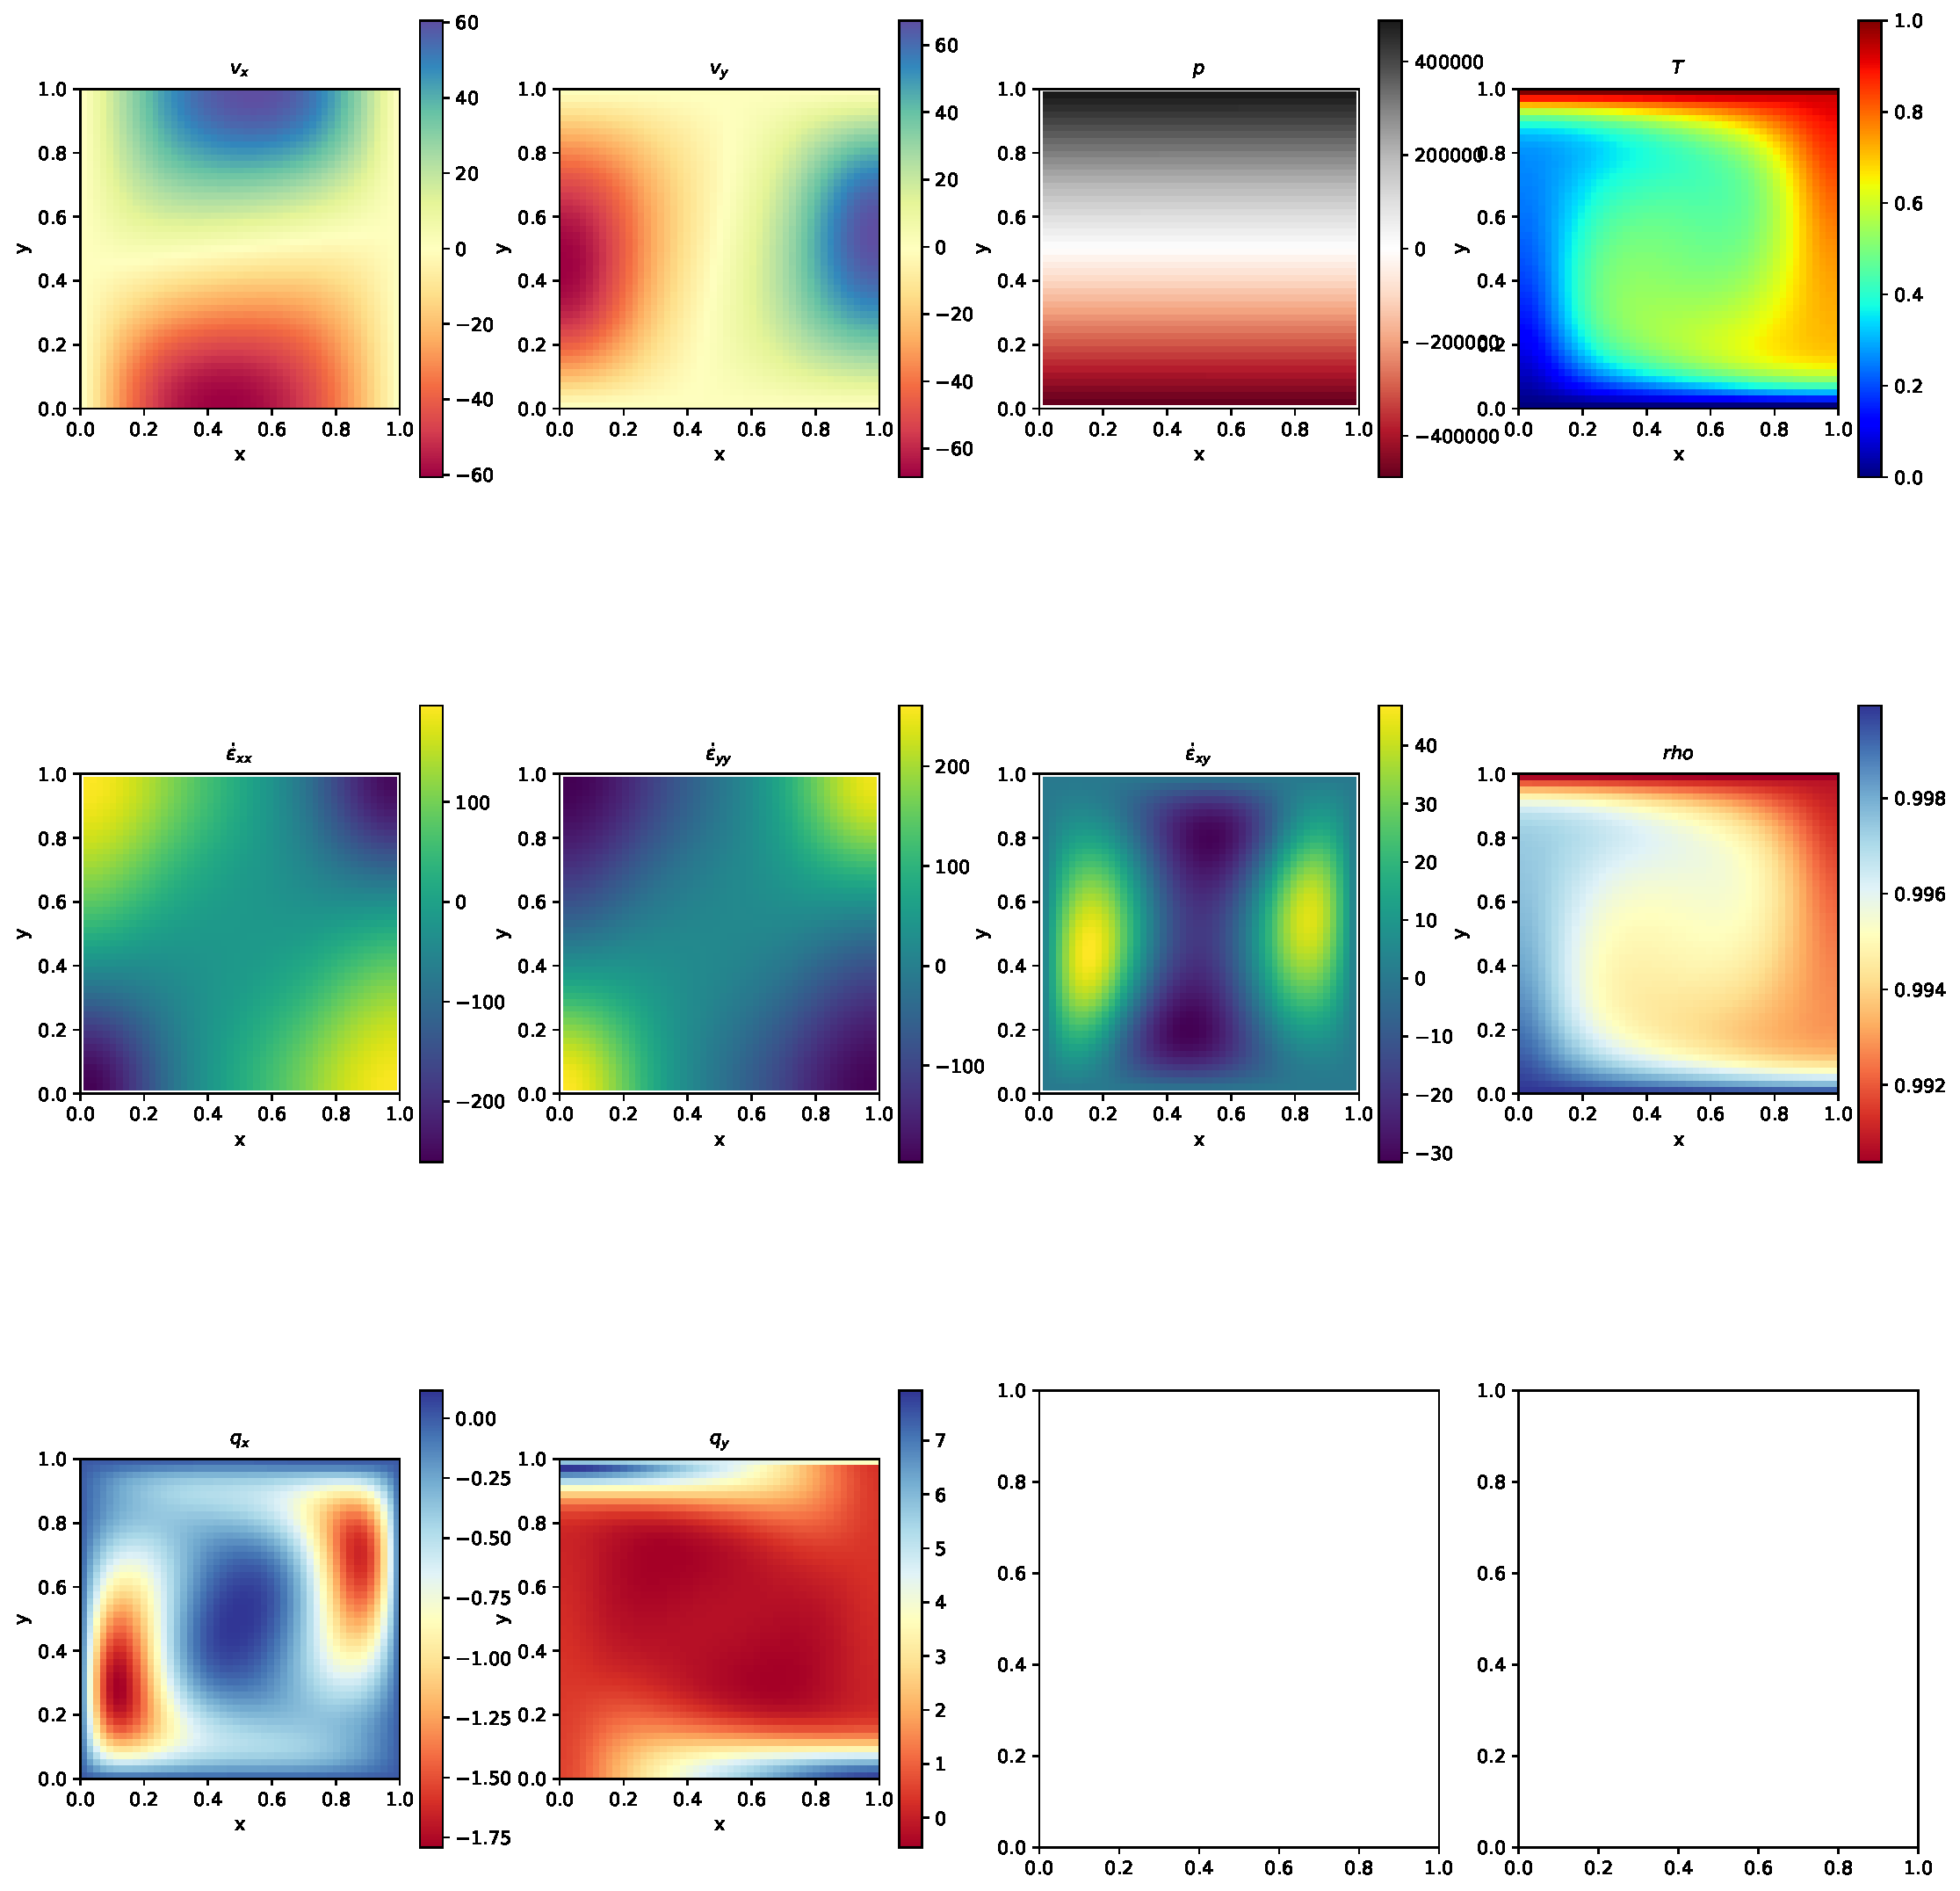
\includegraphics[width=16cm]{python_codes/fieldstone_03/results_1e4/48x48/solution.pdf}\\
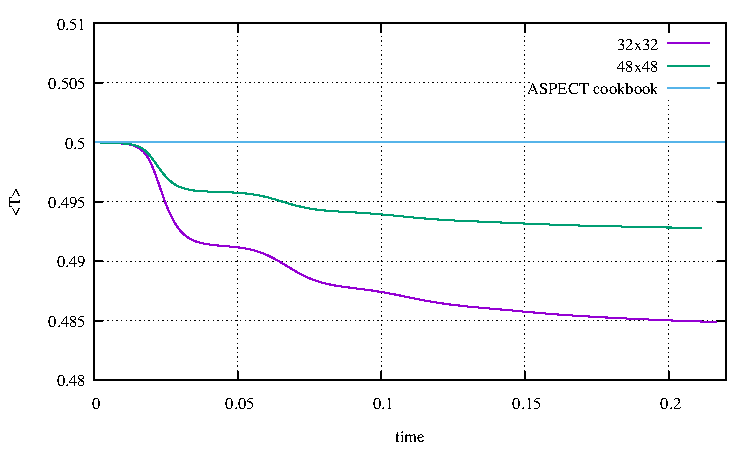
\includegraphics[width=5cm]{python_codes/fieldstone_03/results_1e4/Tavrg.pdf}
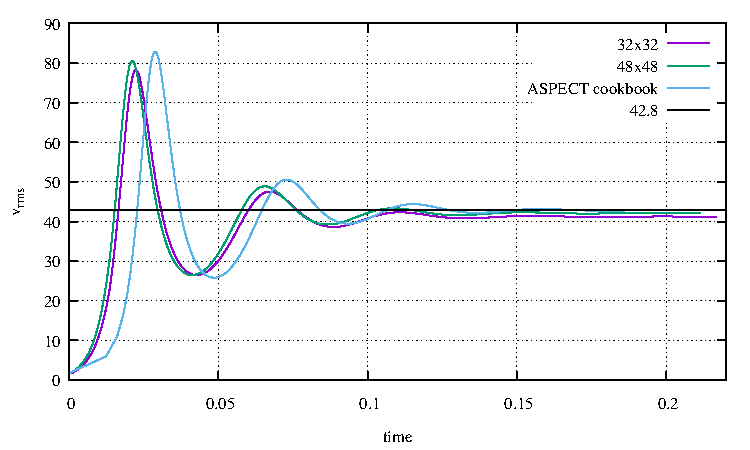
\includegraphics[width=5cm]{python_codes/fieldstone_03/results_1e4/vrms.pdf}\\
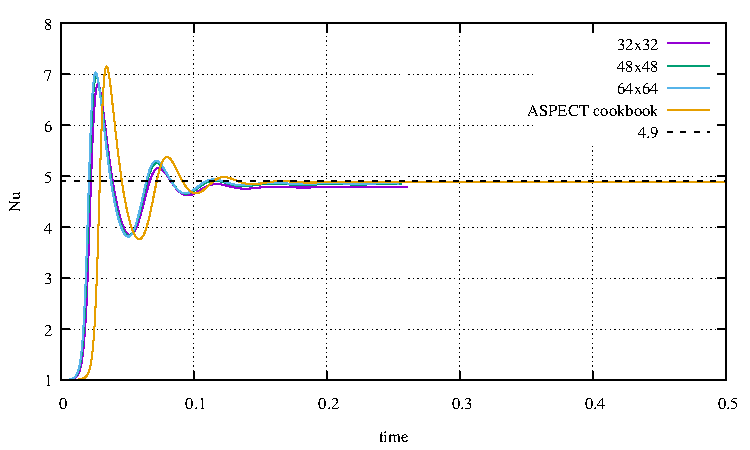
\includegraphics[width=5cm]{python_codes/fieldstone_03/results_1e4/Nu.pdf}
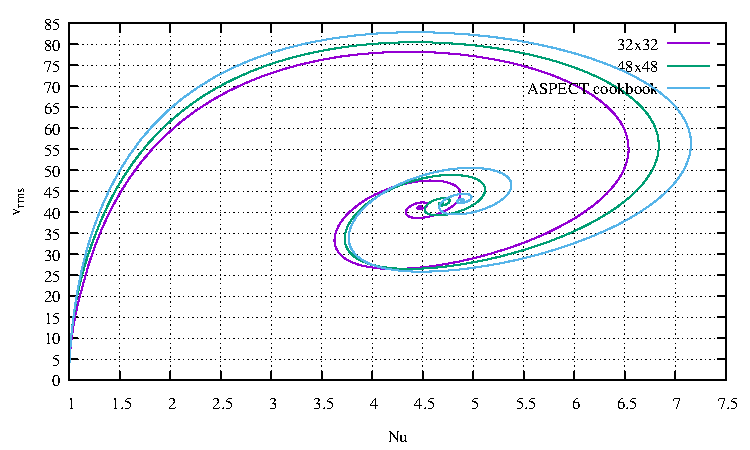
\includegraphics[width=5cm]{python_codes/fieldstone_03/results_1e4/Nu_vrms.pdf}
\end{center}

\newpage
\paragraph{Results for $Ra=10^5$}.
\begin{center}
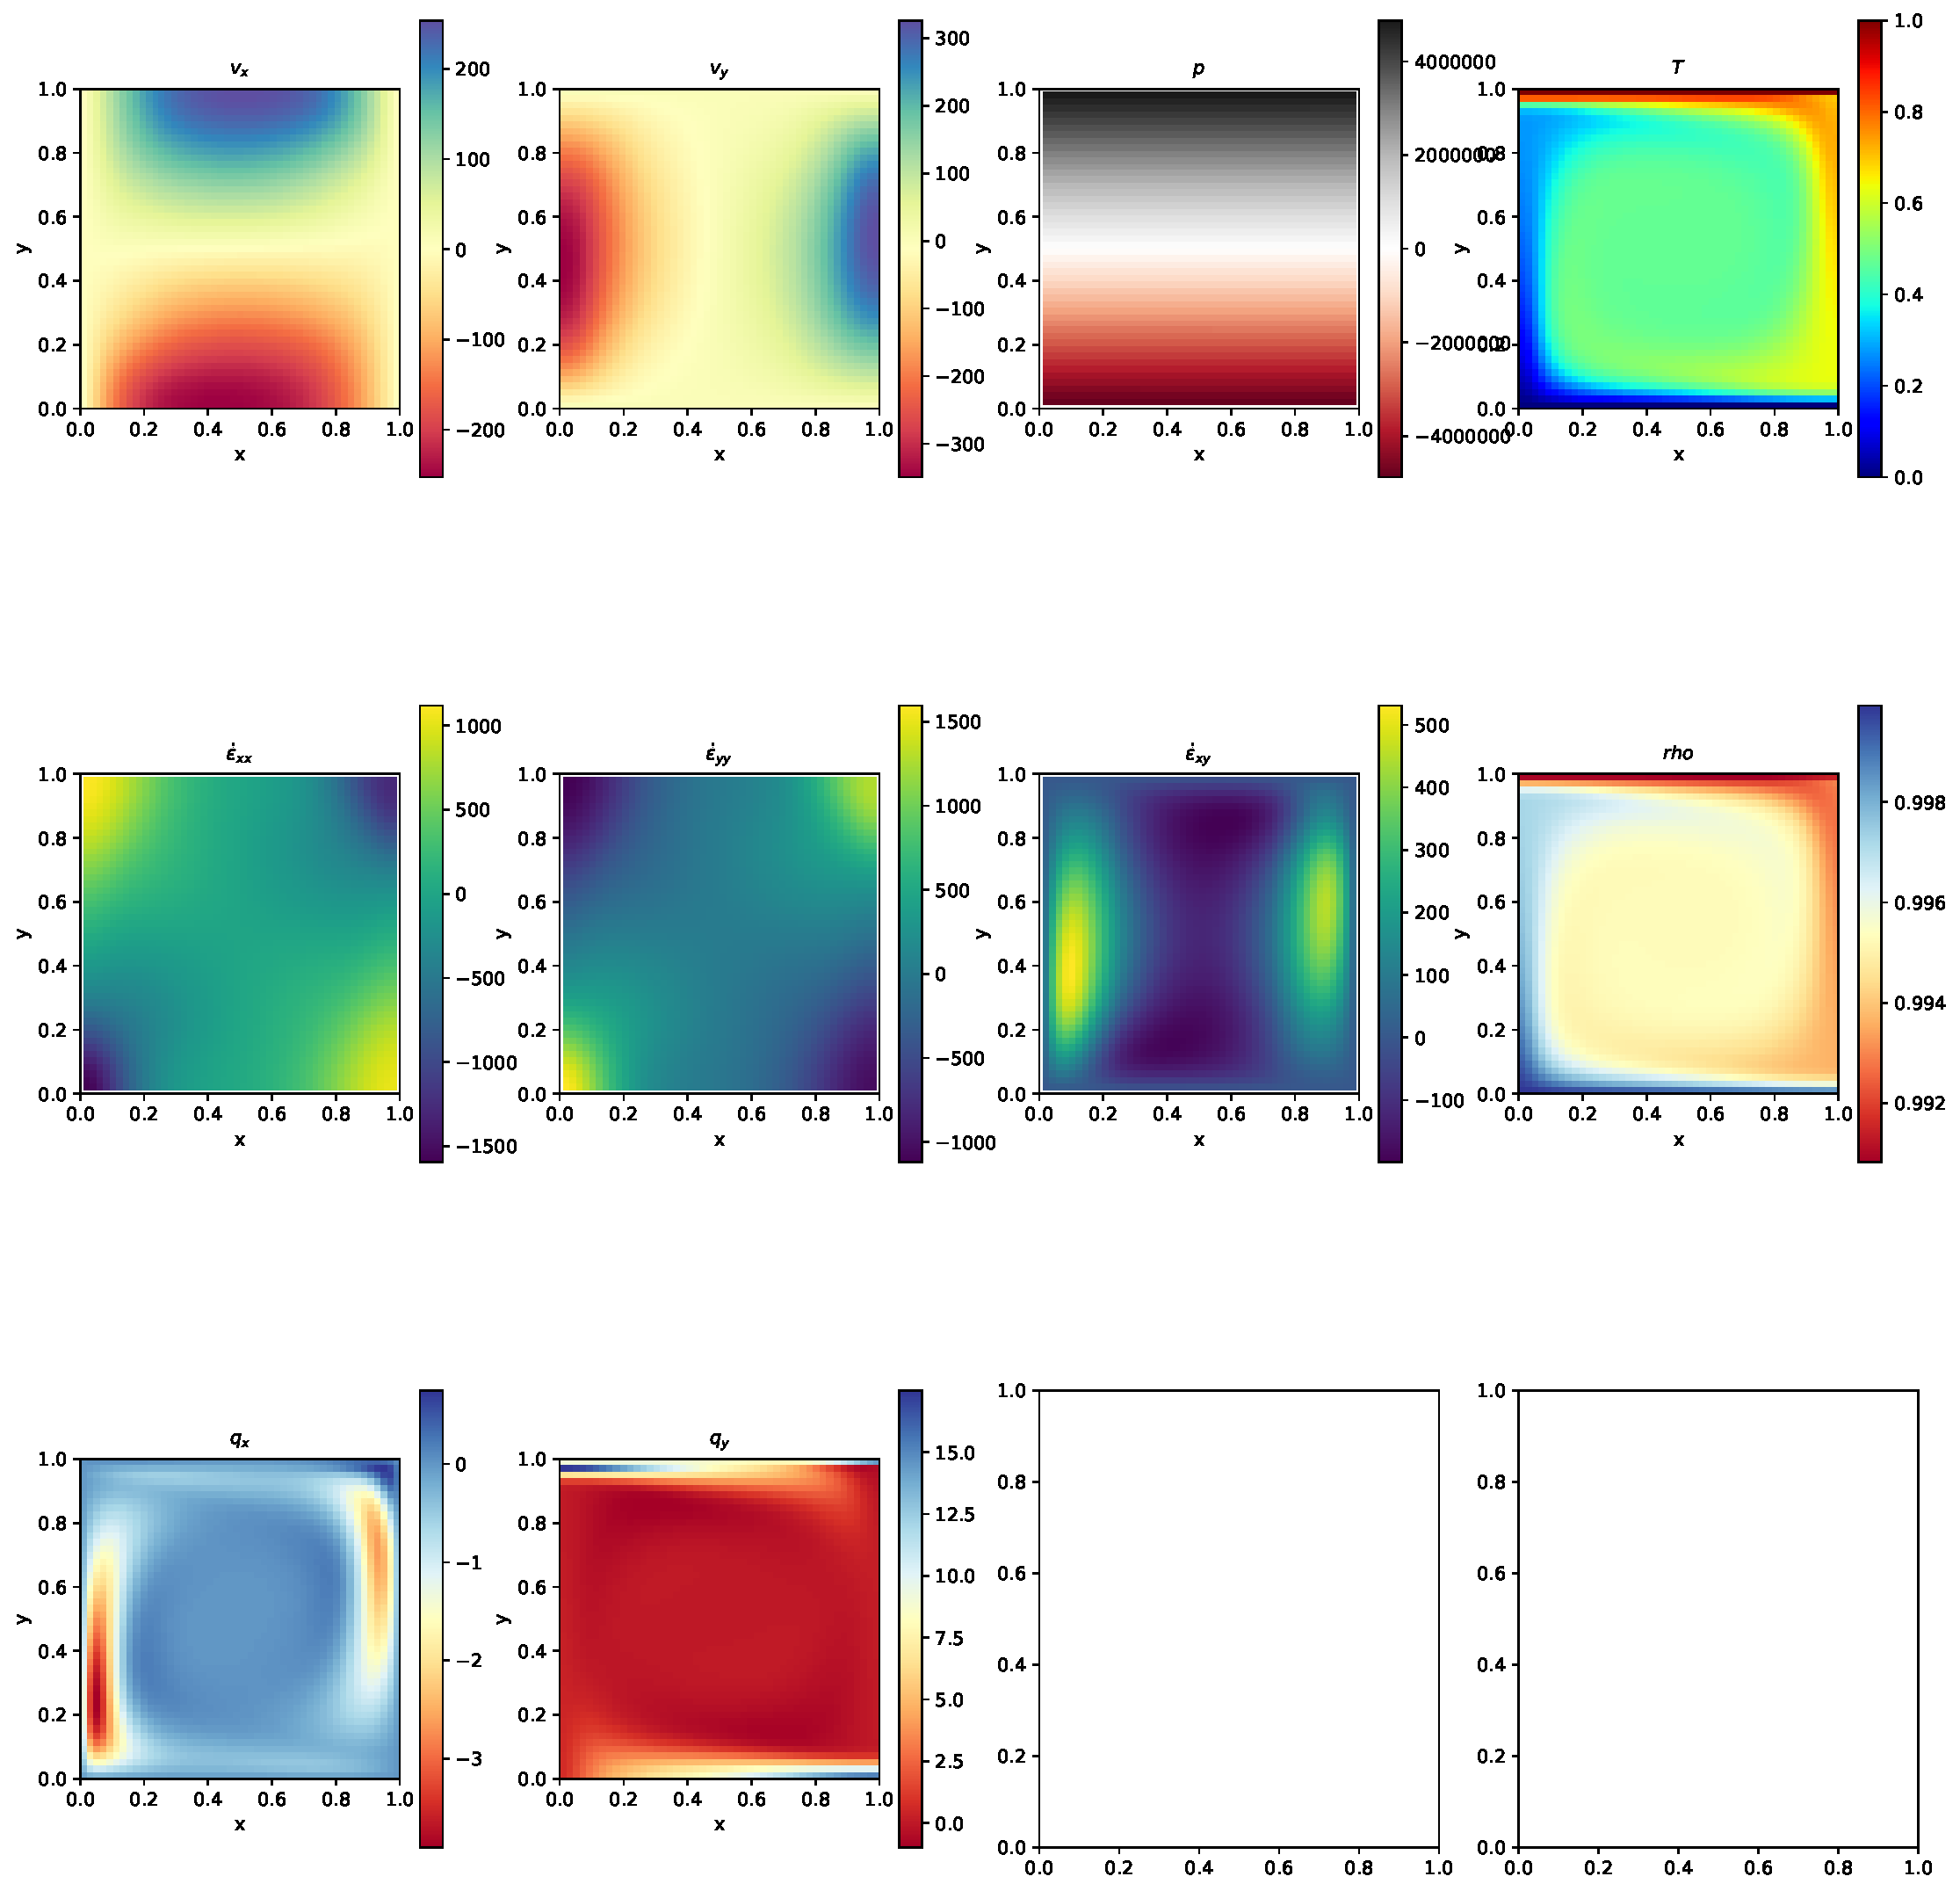
\includegraphics[width=16cm]{python_codes/fieldstone_03/results_1e5/48x48/solution.pdf}\\
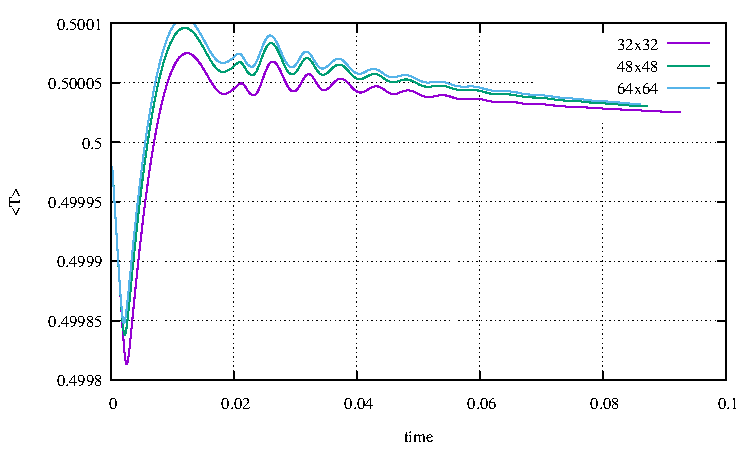
\includegraphics[width=5cm]{python_codes/fieldstone_03/results_1e5/Tavrg.pdf}
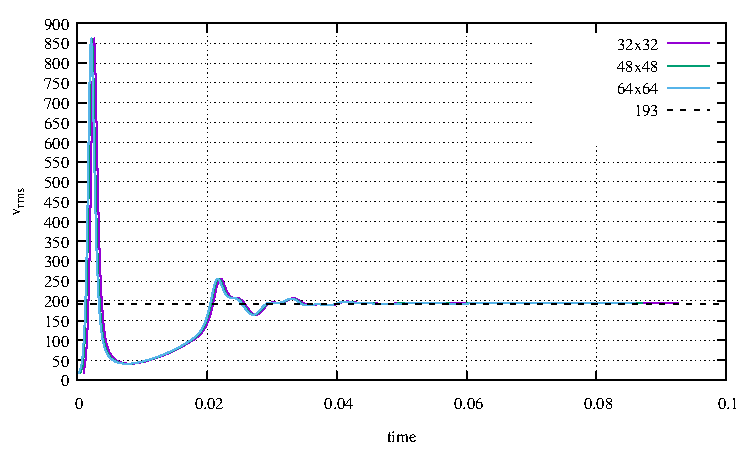
\includegraphics[width=5cm]{python_codes/fieldstone_03/results_1e5/vrms.pdf}\\
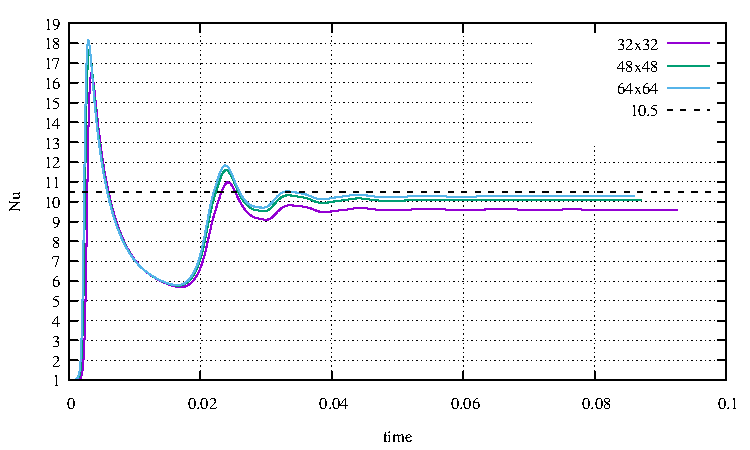
\includegraphics[width=5cm]{python_codes/fieldstone_03/results_1e5/Nu.pdf}
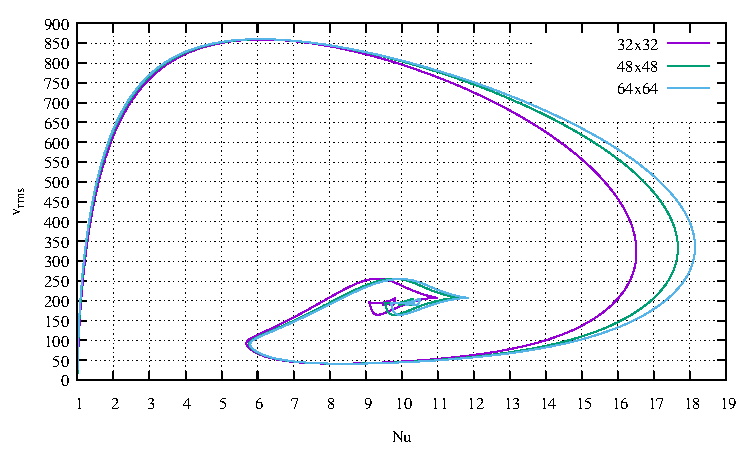
\includegraphics[width=5cm]{python_codes/fieldstone_03/results_1e5/Nu_vrms.pdf}
\end{center}

\newpage
\paragraph{Results for $Ra=10^6$}.
\begin{center}
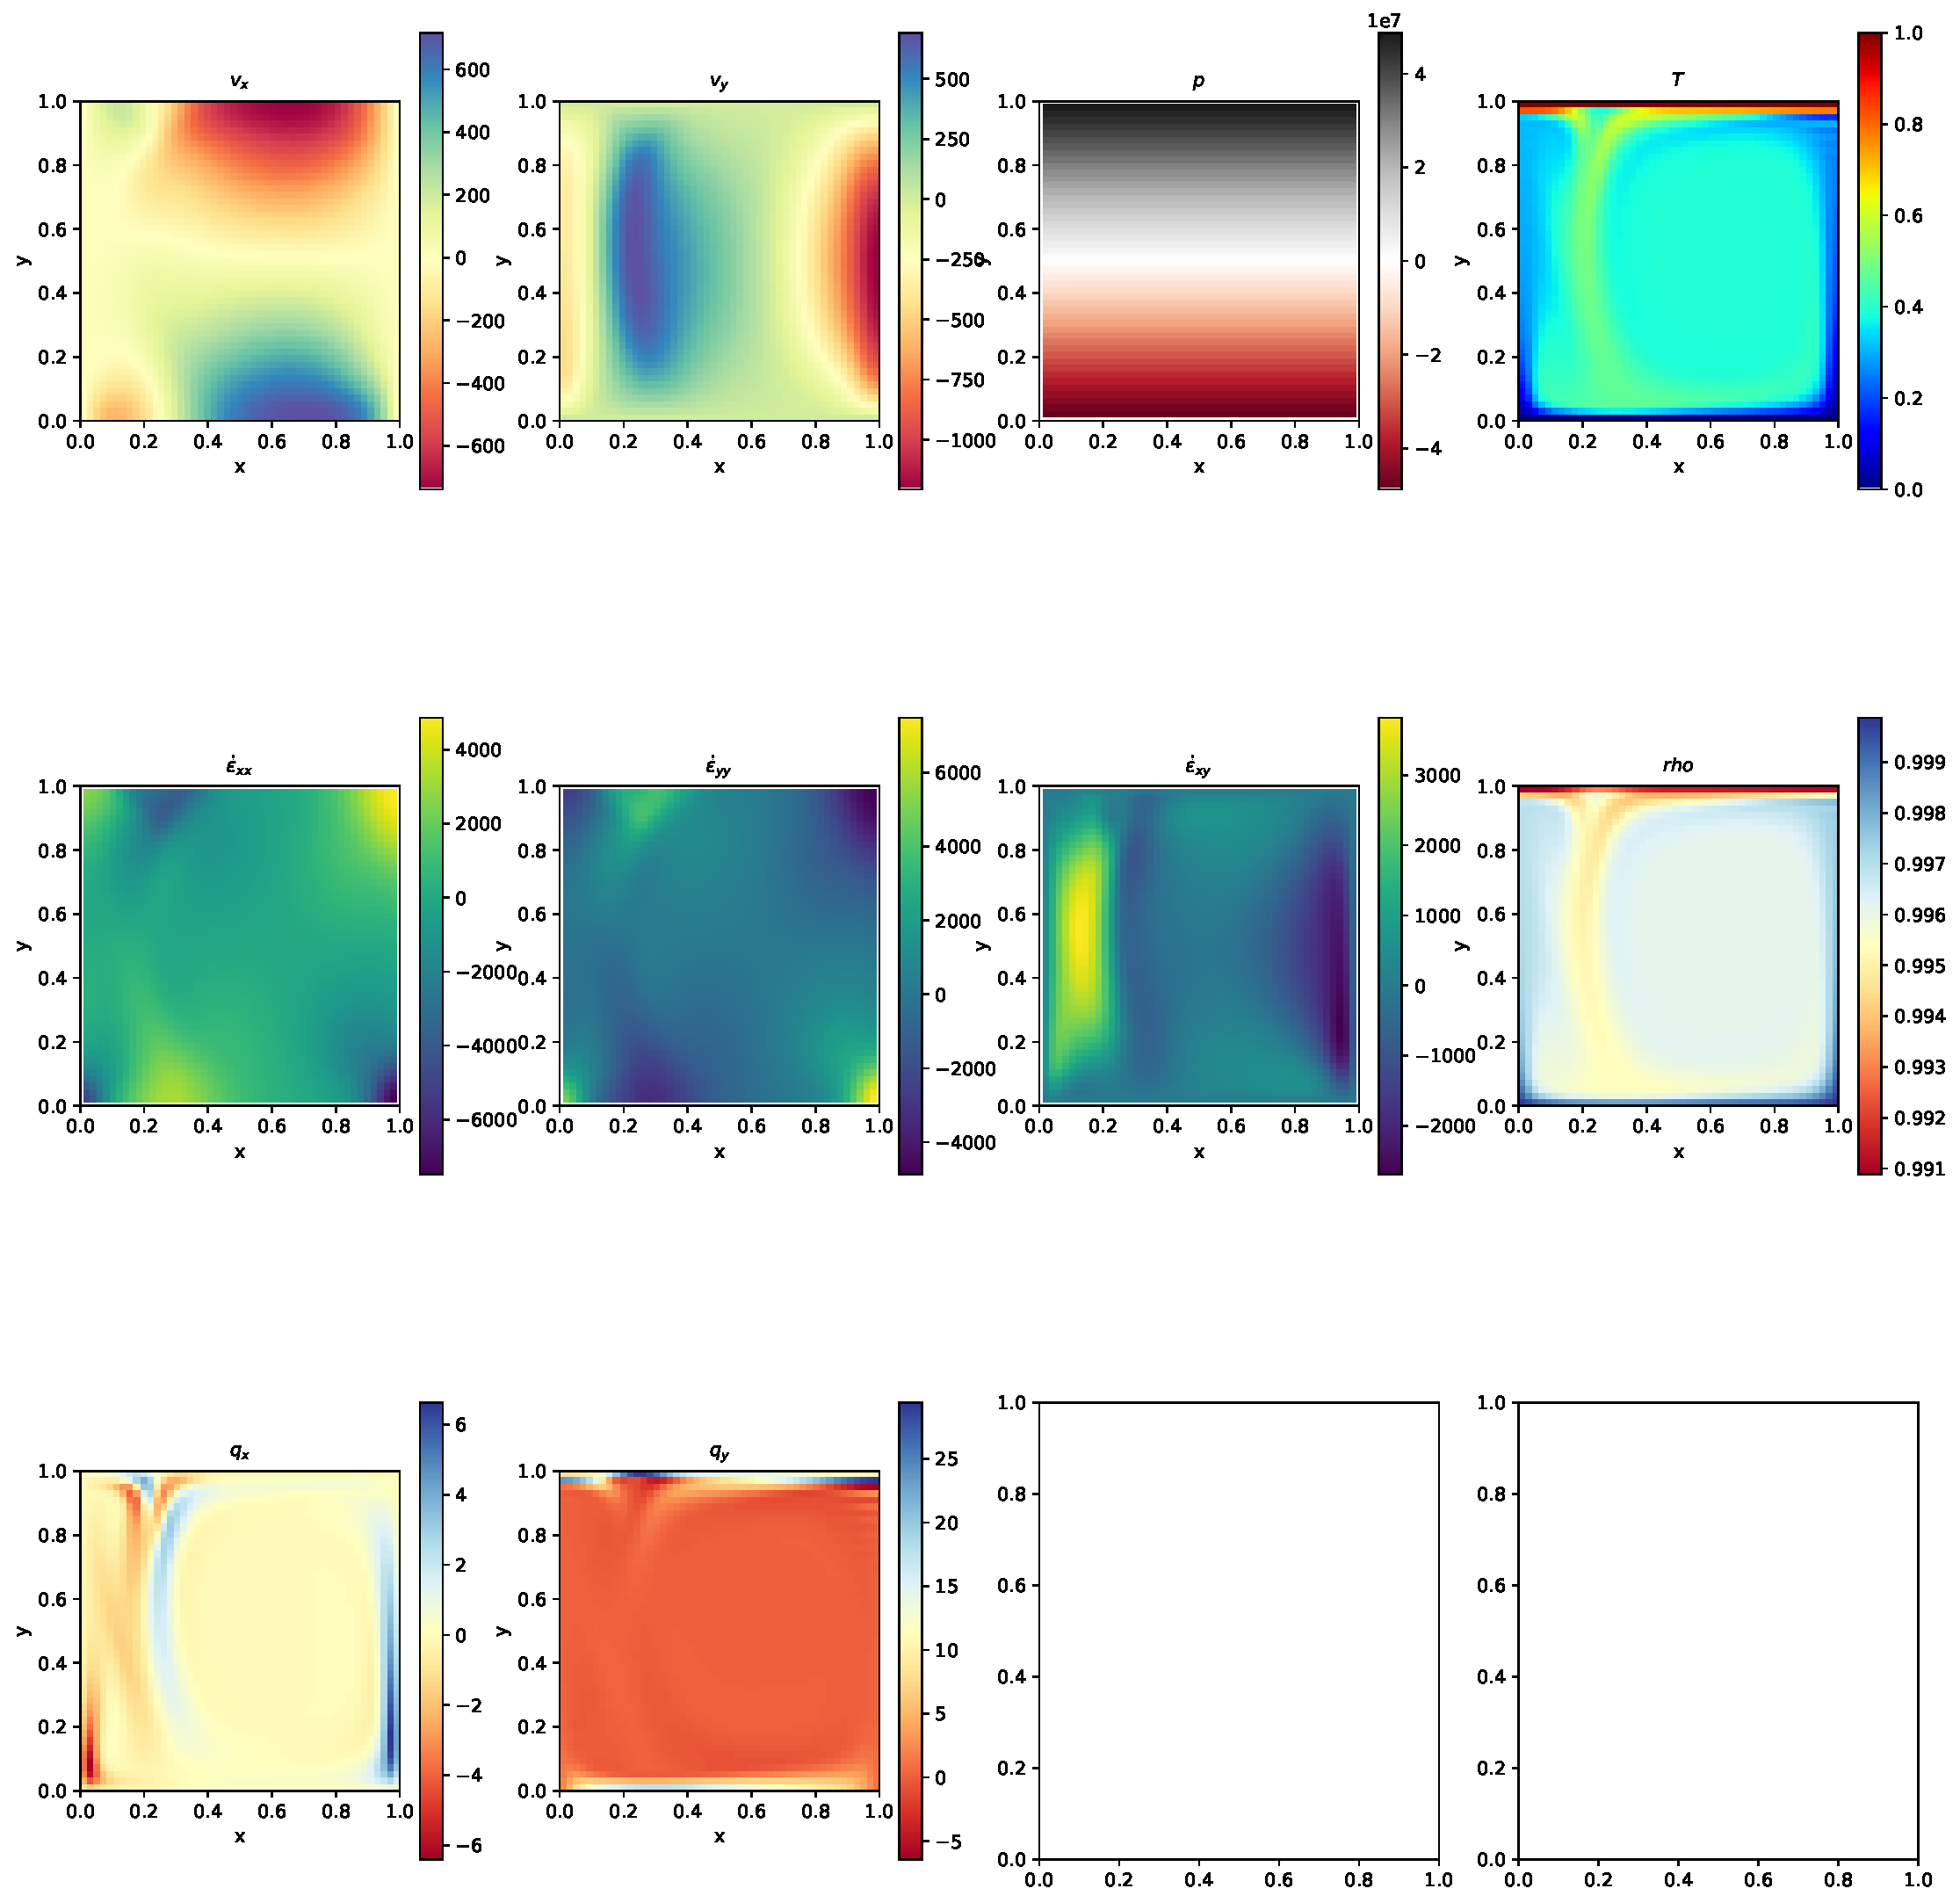
\includegraphics[width=16cm]{python_codes/fieldstone_03/results_1e6/48x48/solution.pdf}\\
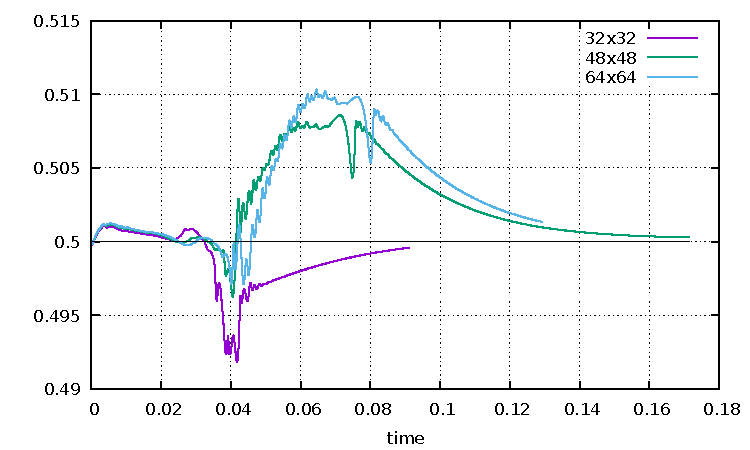
\includegraphics[width=5cm]{python_codes/fieldstone_03/results_1e6/Tavrg.pdf}
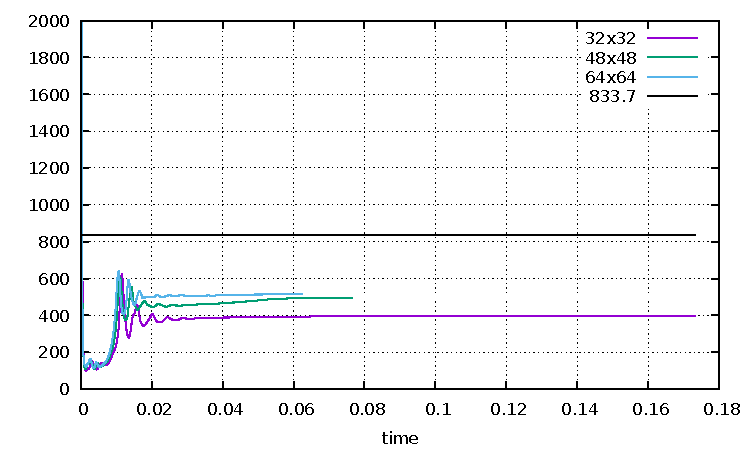
\includegraphics[width=5cm]{python_codes/fieldstone_03/results_1e6/vrms.pdf}\\
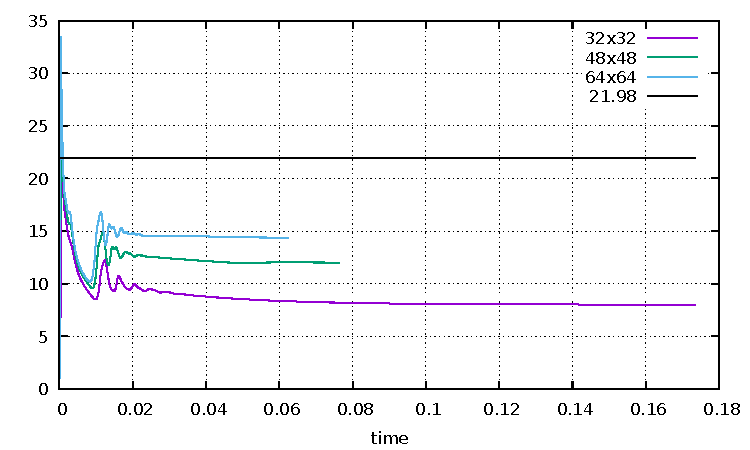
\includegraphics[width=5cm]{python_codes/fieldstone_03/results_1e6/Nu.pdf}
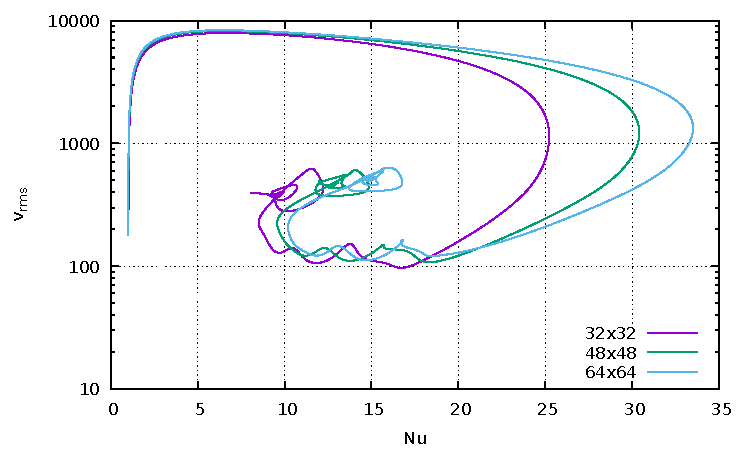
\includegraphics[width=5cm]{python_codes/fieldstone_03/results_1e6/Nu_vrms.pdf}
\end{center}


I have tested the influence of the CFL number (0.5 instead of 1) and it does not change much at all.





 %%%%%%%%%%%%%%%%%%%%%%%%%%%%%%%%%%%%%%%%%%%%%%%%%

\newpage %%%%%%%%%%%%%%%%%%%%%%%%%%%%%%%%%%%%%%%%%%%%%%%%%%%%%%%%%%%%%%%%%%%%%%%%%%%%%%%%
\section*{
Stone 04: The lid driven cavity 
\label{f04}}
\addcontentsline{toc}{section}{\protect\numberline{} 
Stone 04: The lid driven cavity 
}


The lid driven cavity is a famous Computational Fluid Dynamics test case and 
has been studied in countless publications with a wealth of numerical techniques
(see \cite{ertu09} for a succinct review) and also in the laboratory \cite{kost84}.

It models a plane flow of an isothermal isoviscous fluid in a rectangular (usually square) lid-driven cavity. 
The boundary conditions are indicated in the Fig. \ref{fig_ldc}a. The gravity is set to zero.

%---------------------------------------------------------
\subsection{the lid driven cavity problem ({\tt ldc=0})}
In the standard case, the upper side of the cavity moves in its own plane at unit speed, while the other sides are fixed.
This thereby introduces a discontinuity in the boundary conditions at the two upper corners of the cavity and yields
an uncertainty as to which boundary (side or top) the corner points belong to. 
In this version of the code the top corner nodes are considered to be part of the lid. If these are excluded 
the recovered pressure showcases and extremely large checkboard pattern.

This benchmark is usually dicussed in the context of low to very high Reynolds number with the full 
Navier-Stokes equations being solved (with the noticeable exception of \cite{sagl81a,sagl81b,chpc95,eid2005}
which focus on the Stokes equation). 
In the case of the incompressible Stokes flow, 
the absence of inertia renders this problem instantaneous so that only one time step is needed.

%---------------------------------------------------------
\subsection{the lid driven cavity problem - regularisation I ({\tt ldc=1})}

We avoid the top corner nodes issue altogether by  
prescribing the horizontal velocity of the lid as follows: 
\begin{equation}
u(x)=x^2(1-x)^2.
\end{equation}
In this case the velocity and its first derivative is continuous at the corners. This is the so-called regularised lid-driven cavity problem \cite{piva94}.

%---------------------------------------------------------
\subsection{the lid driven cavity problem - regularisation II ({\tt ldc=2})}

Another regularisation was presented in \cite{dejn16}. 
Here, a regularized lid driven cavity is studied which is consistent in the sense that 
${\bm \nabla}\cdot{\bm v}=0$ 
holds also at the corners of the domain.
There are no-slip conditions at the boundaries $x=0$, $x=1$, and $y=0$. 

The velocity at $y=1$ is given by

\begin{eqnarray}
u(x) &=& 1-\frac{1}{4}\left( 1-\cos (\frac{x_1-x}{x_1}\pi)  \right)^2   \quad\quad x\in[0,x_1] \nonumber\\
u(x) &=& 1 \quad\quad x\in[x_1,1-x_1] \nonumber\\
u(x) &=& 1-\frac{1}{4}\left( 1-\cos (\frac{x-(1-x_1)}{x_1}\pi)  \right)^2   \quad\quad x\in[1-x_1,1]
\end{eqnarray}
Results are obtained with $x_1=0.1$.

\begin{center}
\fbox{
\parbox{10cm}{{\bf features}
\begin{itemize}
\item $Q_1\times P_0$ element \index{$Q_1 \times P_0$}
\item incompressible flow
\item penalty formulation \index{penalty formulation}
\item isothermal \index{isothermal}
\item isoviscous \index{isoviscous}
\end{itemize}
}}
\end{center}



\newpage
A 100x100 element grid is used. No-slip boundary conditions are prescribed on sides and
bottom. A zero vertical velocity is prescribed at the top and the exact form of the 
prescribed horizontal velocity is controlled by the {\tt ldc} parameter.

\begin{center}
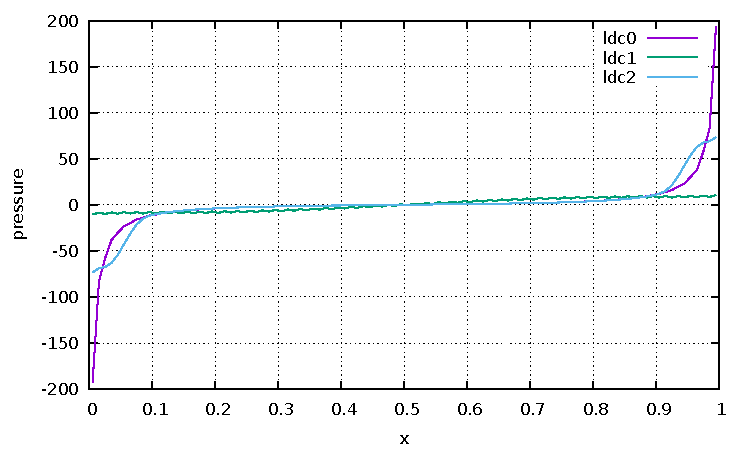
\includegraphics[width=8cm]{python_codes/fieldstone_04/results/p.pdf}\\
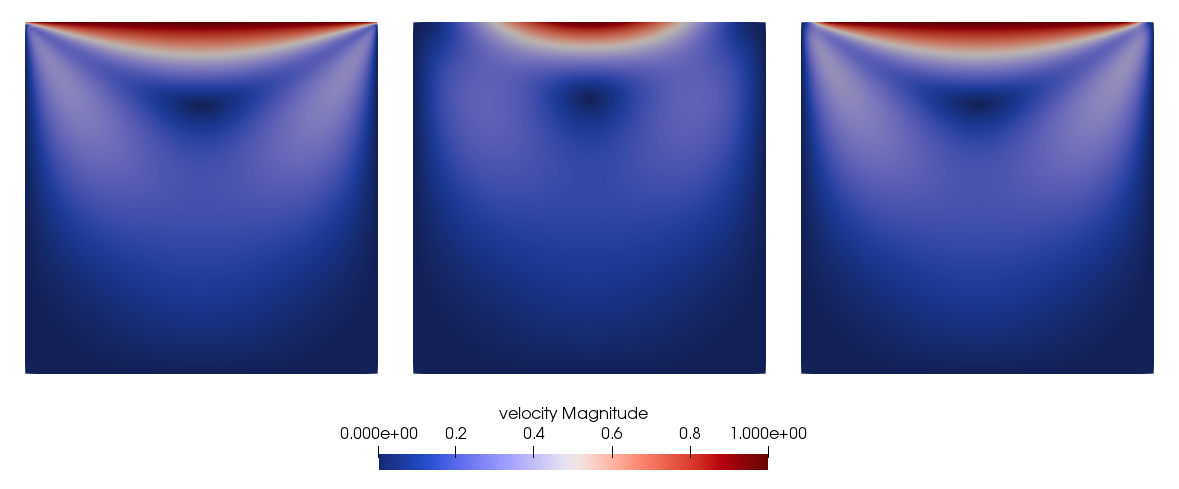
\includegraphics[width=12cm]{python_codes/fieldstone_04/results/velocities}\\
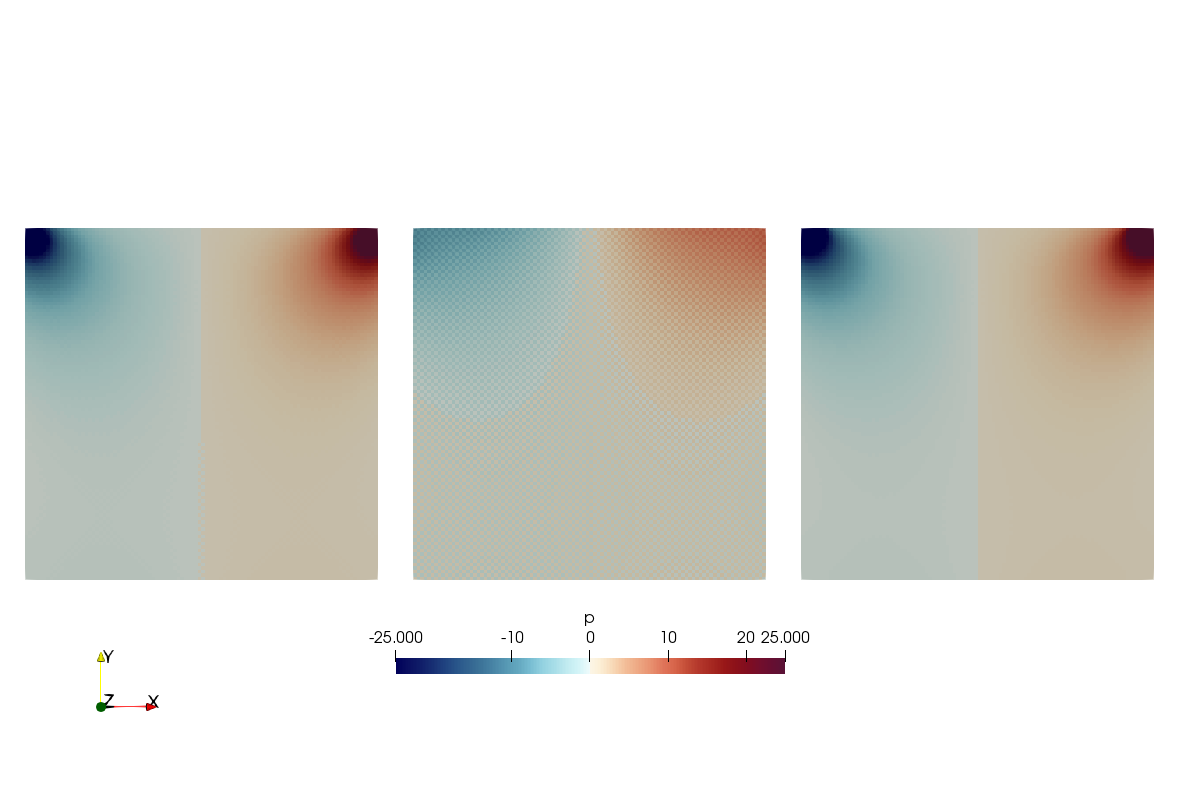
\includegraphics[width=12cm]{python_codes/fieldstone_04/results/pressures}
\end{center}

 %%%%%%%%%%%%%%%%%%%%%%%%%%%%%%%%%%%%%%%%%%%%%%%%%

\newpage %%%%%%%%%%%%%%%%%%%%%%%%%%%%%%%%%%%%%%%%%%%%%%%%%%%%%%%%%%%%%%%%%%%%%%%%%%%%%%%%
\section*{
Stone 05: SolCx benchmark 
\label{f05}}
\addcontentsline{toc}{section}{\protect\numberline{} 
Stone 05: SolCx benchmark 
}
\lstinputlisting[language=bash,basicstyle=\small]{python_codes/fieldstone_05/keywords}

\begin{center}
Code at \url{https://github.com/cedrict/fieldstone/tree/master/python_codes/fieldstone_05}
\end{center}

\par\noindent\rule{\textwidth}{0.4pt}
%%%%%%%%%%%%%%%%%%%%%%%%%%%%%%%%%%%%%%%%%%%%%%%%%%%%%%%%%%%%%%%%%%%%%%%%%%%%%%%%%%%%%%%%%

The experiment is fully described in Section~\ref{ss:solcx}.
The viscosity is prescribed at the quadrature points 
If the number of elements is even in the $x$-direction direction, all elements 
(and their associated quadrature points)
have a constant viscosity ($1$ or  $10^6$). If it is odd, then the elements situated 
at the viscosity jump have half their integration points with $\eta=1$ and half 
with $\eta=10^6$ 
(which is a pathological case since the used quadrature rule inside elements cannot represent 
accurately such a jump).  

\begin{center}
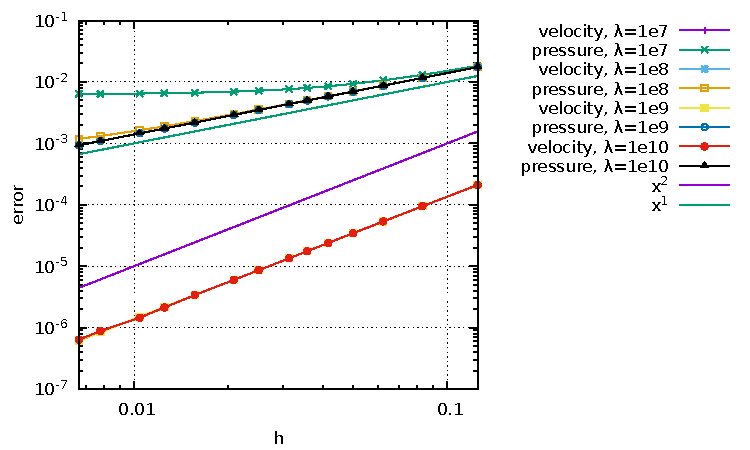
\includegraphics[width=8cm]{python_codes/fieldstone_05/results/errors_even.pdf}
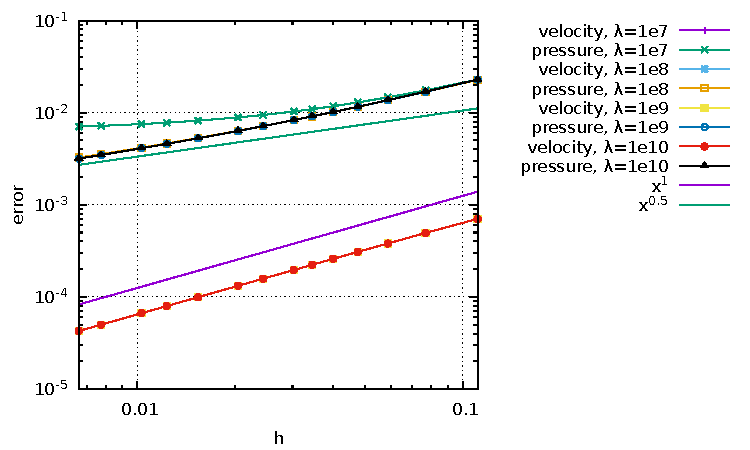
\includegraphics[width=8cm]{python_codes/fieldstone_05/results/errors_odd.pdf}\\
{\captionfont Velocity and pressure error convergence as a function of mesh size and for various values
of the penalty parameter. Left: even number of elements in each direction; Right: odd numbers.
}
\end{center}

Because of the high viscosity in the right part of the domain, the penalty parameter should 
be high enough to insure an incompressible flow and thereby recover the expected convergence rate
(at least for the even case). Note that values higher than $\lambda=10^{10}$ yield erroneous solutions 
due to round-off errors. 

\begin{center}
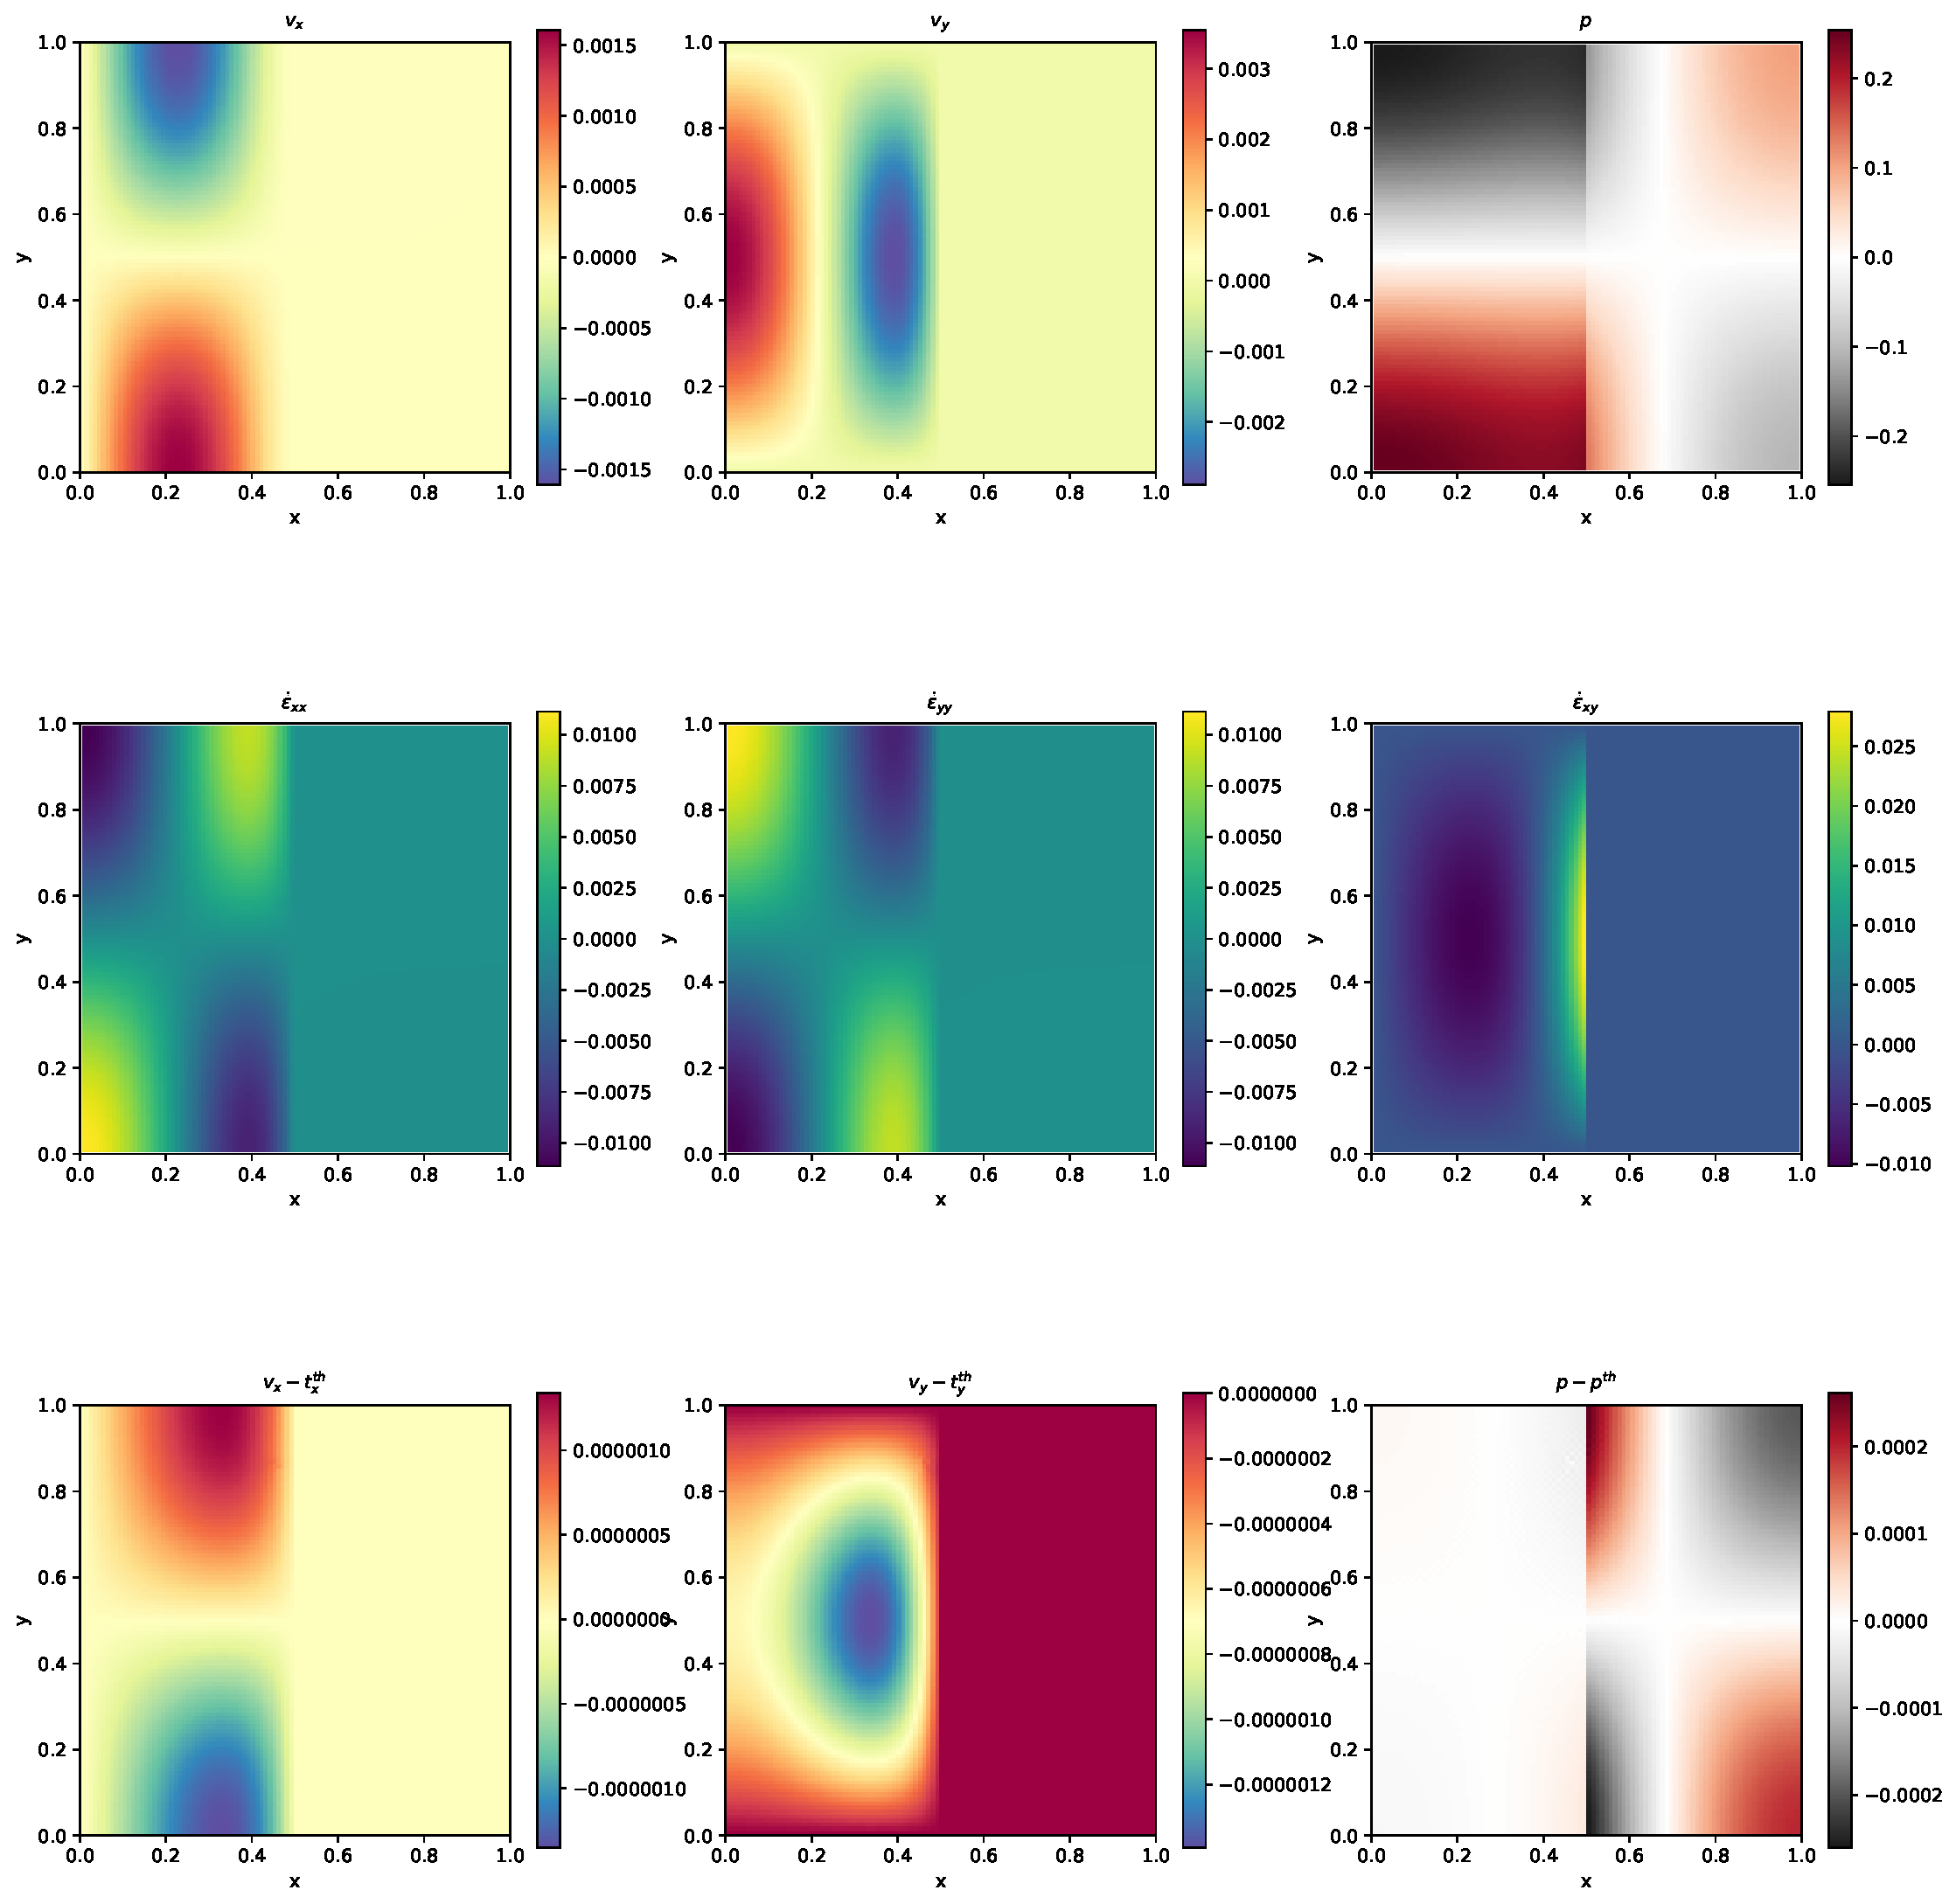
\includegraphics[width=16cm]{python_codes/fieldstone_05/results/solution.pdf}\\
{\captionfont Various fields for 100x100 mesh}
\end{center}


\infortran
Note that a Fortran90 version of this code is available in the same folder. \index{general}{fortran90}


 %%%%%%%%%%%%%%%%%%%%%%%%%%%%%%%%%%%%%%%%%%%%%%%%%

\newpage %%%%%%%%%%%%%%%%%%%%%%%%%%%%%%%%%%%%%%%%%%%%%%%%%%%%%%%%%%%%%%%%%%%%%%%%%%%%%%%%
\section*{
Stone 06: SolKz benchmark 
\label{f06}}
\addcontentsline{toc}{section}{\protect\numberline{} 
Stone 06: SolKz benchmark 
}
\lstinputlisting[language=bash,basicstyle=\small]{python_codes/fieldstone_06/keywords}

\begin{center}
Code at \url{https://github.com/cedrict/fieldstone/tree/master/python_codes/fieldstone_06}
\end{center}

\par\noindent\rule{\textwidth}{0.4pt}
%%%%%%%%%%%%%%%%%%%%%%%%%%%%%%%%%%%%%%%%%%%%%%%%%%%%%%%%%%%%%%%%%%%%%%%%%%%%%%%%%%%%%%%%%

The SolKz benchmark \cite{repa87} is similar to the SolCx benchmark.
but the viscosity is now a function of the space coordinates: 
\begin{equation}
\eta(y)=\exp(By) \quad {\rm with} \quad B=13.8155
\end{equation}
It is however not a discontinuous function but grows exponentially with the vertical coordinate so that its overall variation is again $10^6$. 
The forcing is again chosen by imposing a spatially variable density variation as follows:
\begin{equation}
\rho(x,y)=\sin(2y) \cos(3\pi x)
\end{equation}
Free slip boundary conditions are imposed on all sides of the domain.
This benchmark is presented in Zhong (1996) \cite{zhon96} as well and is studied 
in Duretz \etal (2011) \cite{dumg11} and Gerya \etal (2013) \cite{gemd13}.

\begin{center}
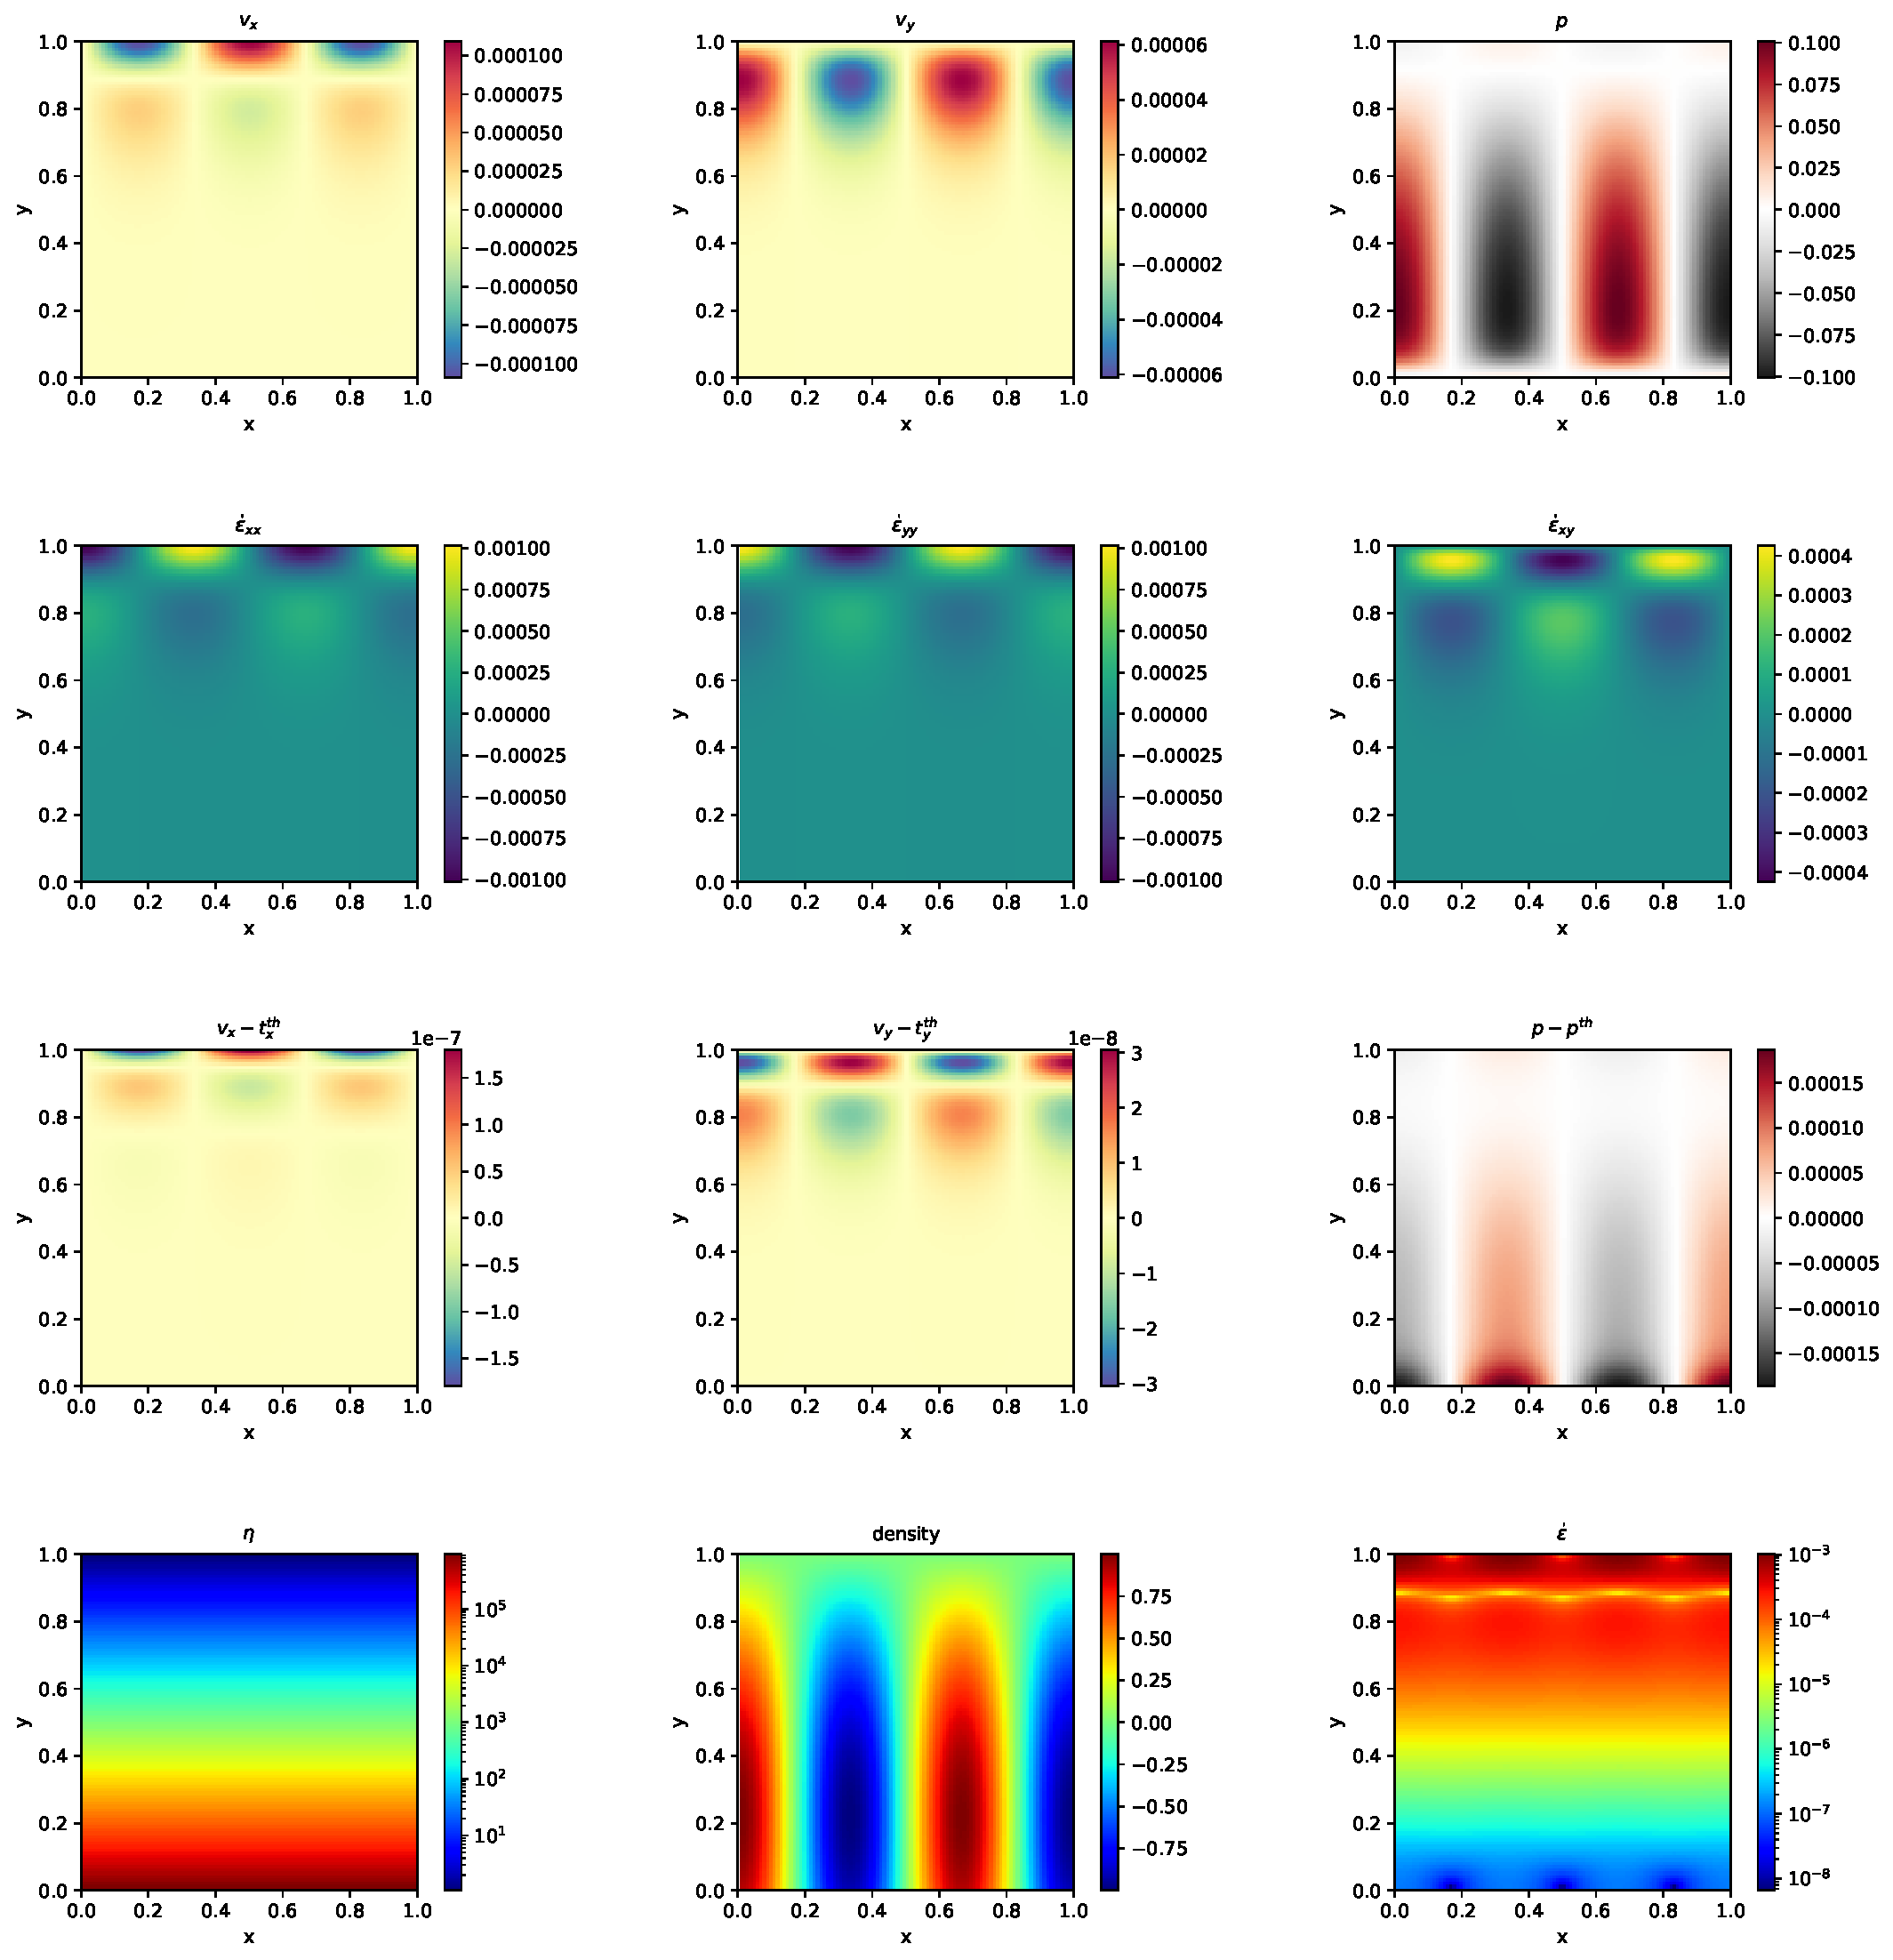
\includegraphics[width=14cm]{python_codes/fieldstone_06/results/solution.pdf}
\end{center}

\begin{center}
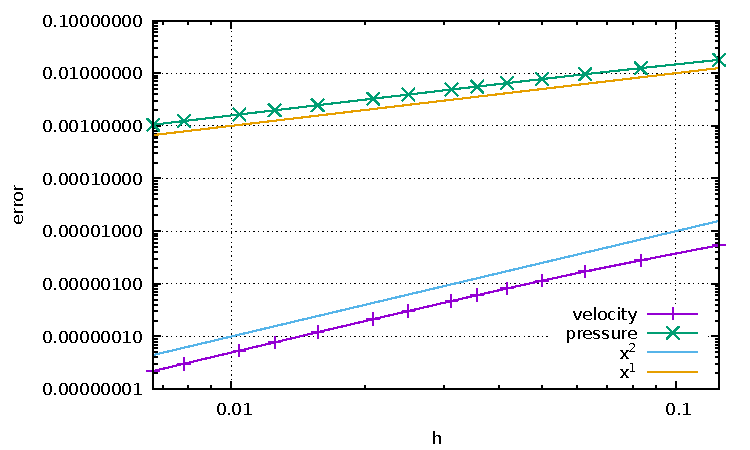
\includegraphics[width=10cm]{python_codes/fieldstone_06/results/errors.pdf}\\
{\captionfont Velocity and pressure error as a function of mesh size.}
\end{center}
 %%%%%%%%%%%%%%%%%%%%%%%%%%%%%%%%%%%%%%%%%%%%%%%%%

\newpage %%%%%%%%%%%%%%%%%%%%%%%%%%%%%%%%%%%%%%%%%%%%%%%%%%%%%%%%%%%%%%%%%%%%%%%%%%%%%%%%
\section*{
Stone 07: SolVi benchmark 
\label{f07}}
\addcontentsline{toc}{section}{\protect\numberline{} 
Stone 07: SolVi benchmark 
}

Following SolCx and SolKz, the SolVi inclusion benchmark solves 
a problem with a discontinuous viscosity field, but in this case 
the viscosity field is chosen in such a way that the discontinuity 
is along a circle. Given the regular nature of the grid used by a majority of codes and the present one, 
this ensures that the discontinuity in the viscosity never aligns to cell boundaries.
This in turns leads to almost discontinuous pressures along the interface which are difficult to represent accurately.
Schmid \& Podlachikov (2003) \cite{scpo03} derived a simple analytic solution for the pressure and 
velocity fields for a circular 
inclusion under simple shear and it was used in \cite{deka08,sunh10,dumg11,krhb12,gemd13}.

Because of the symmetry of the problem, we only have to solve over the top right quarter of the domain.
The analytical solution requires a strain rate boundary condition (e.g., pure shear) to be applied far away 
from the inclusion. In order to avoid using very large domains and/or dealing with this type of boundary condition 
altogether, the analytical solution is evaluated and imposed on the boundaries of the domain. 
By doing so, the truncation error introduced while discretizing the strain rate boundary condition is removed.

A characteristic of the analytic solution is that the pressure is zero inside the inclusion, while outside it follows the relation
\begin{equation}
p_m = 4 \dot{\epsilon}
\frac{\mu_m(\mu_i-\mu_m)}{\mu_i+\mu_m}
\frac{r_i^2}{r^2} \cos(2\theta)
\end{equation}
where $\mu_i = 10^3$ is the viscosity of the inclusion and $\mu_m = 1$ is the viscosity of the background media, $\theta=\tan^{-1}(y/x)$,
and $\dot{\epsilon}=1$ is the applied strain rate.

Deubelbeiss \& Kauss (2008) \cite{deka08} thoroughly investigated this problem with various 
numerical methods (FEM, FDM), with and without tracers, 
and conclusively showed how various averagings lead to different results. 
Duretz et al (2011) \cite{dumg11} obtained a first order convergence for both pressure and velocity, 
while Kronbichler et al (2012) \cite{krhb12}
and Gerya et al (2013) \cite{gemd13} showed that the use of adaptive mesh refinement in respectively the FEM and FDM 
yields convergence rates which depend on refinement strategies. 

\begin{center}
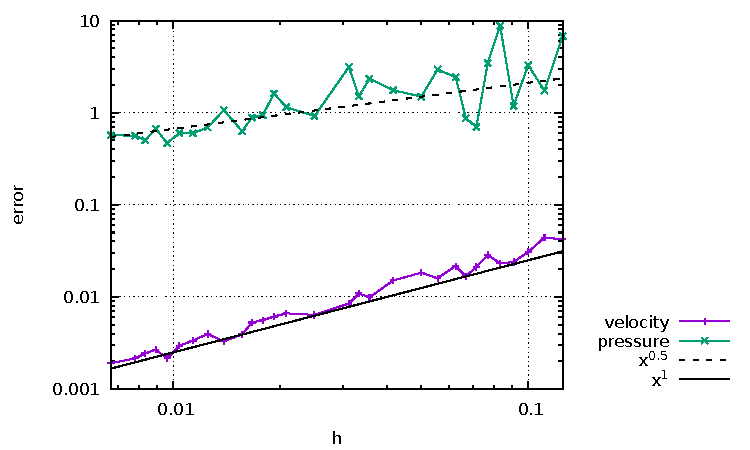
\includegraphics[width=8cm]{python_codes/fieldstone_07/results/errors}\\
{\captionfont Velocity and pressure error convergence as a function of mesh size.}
\end{center}

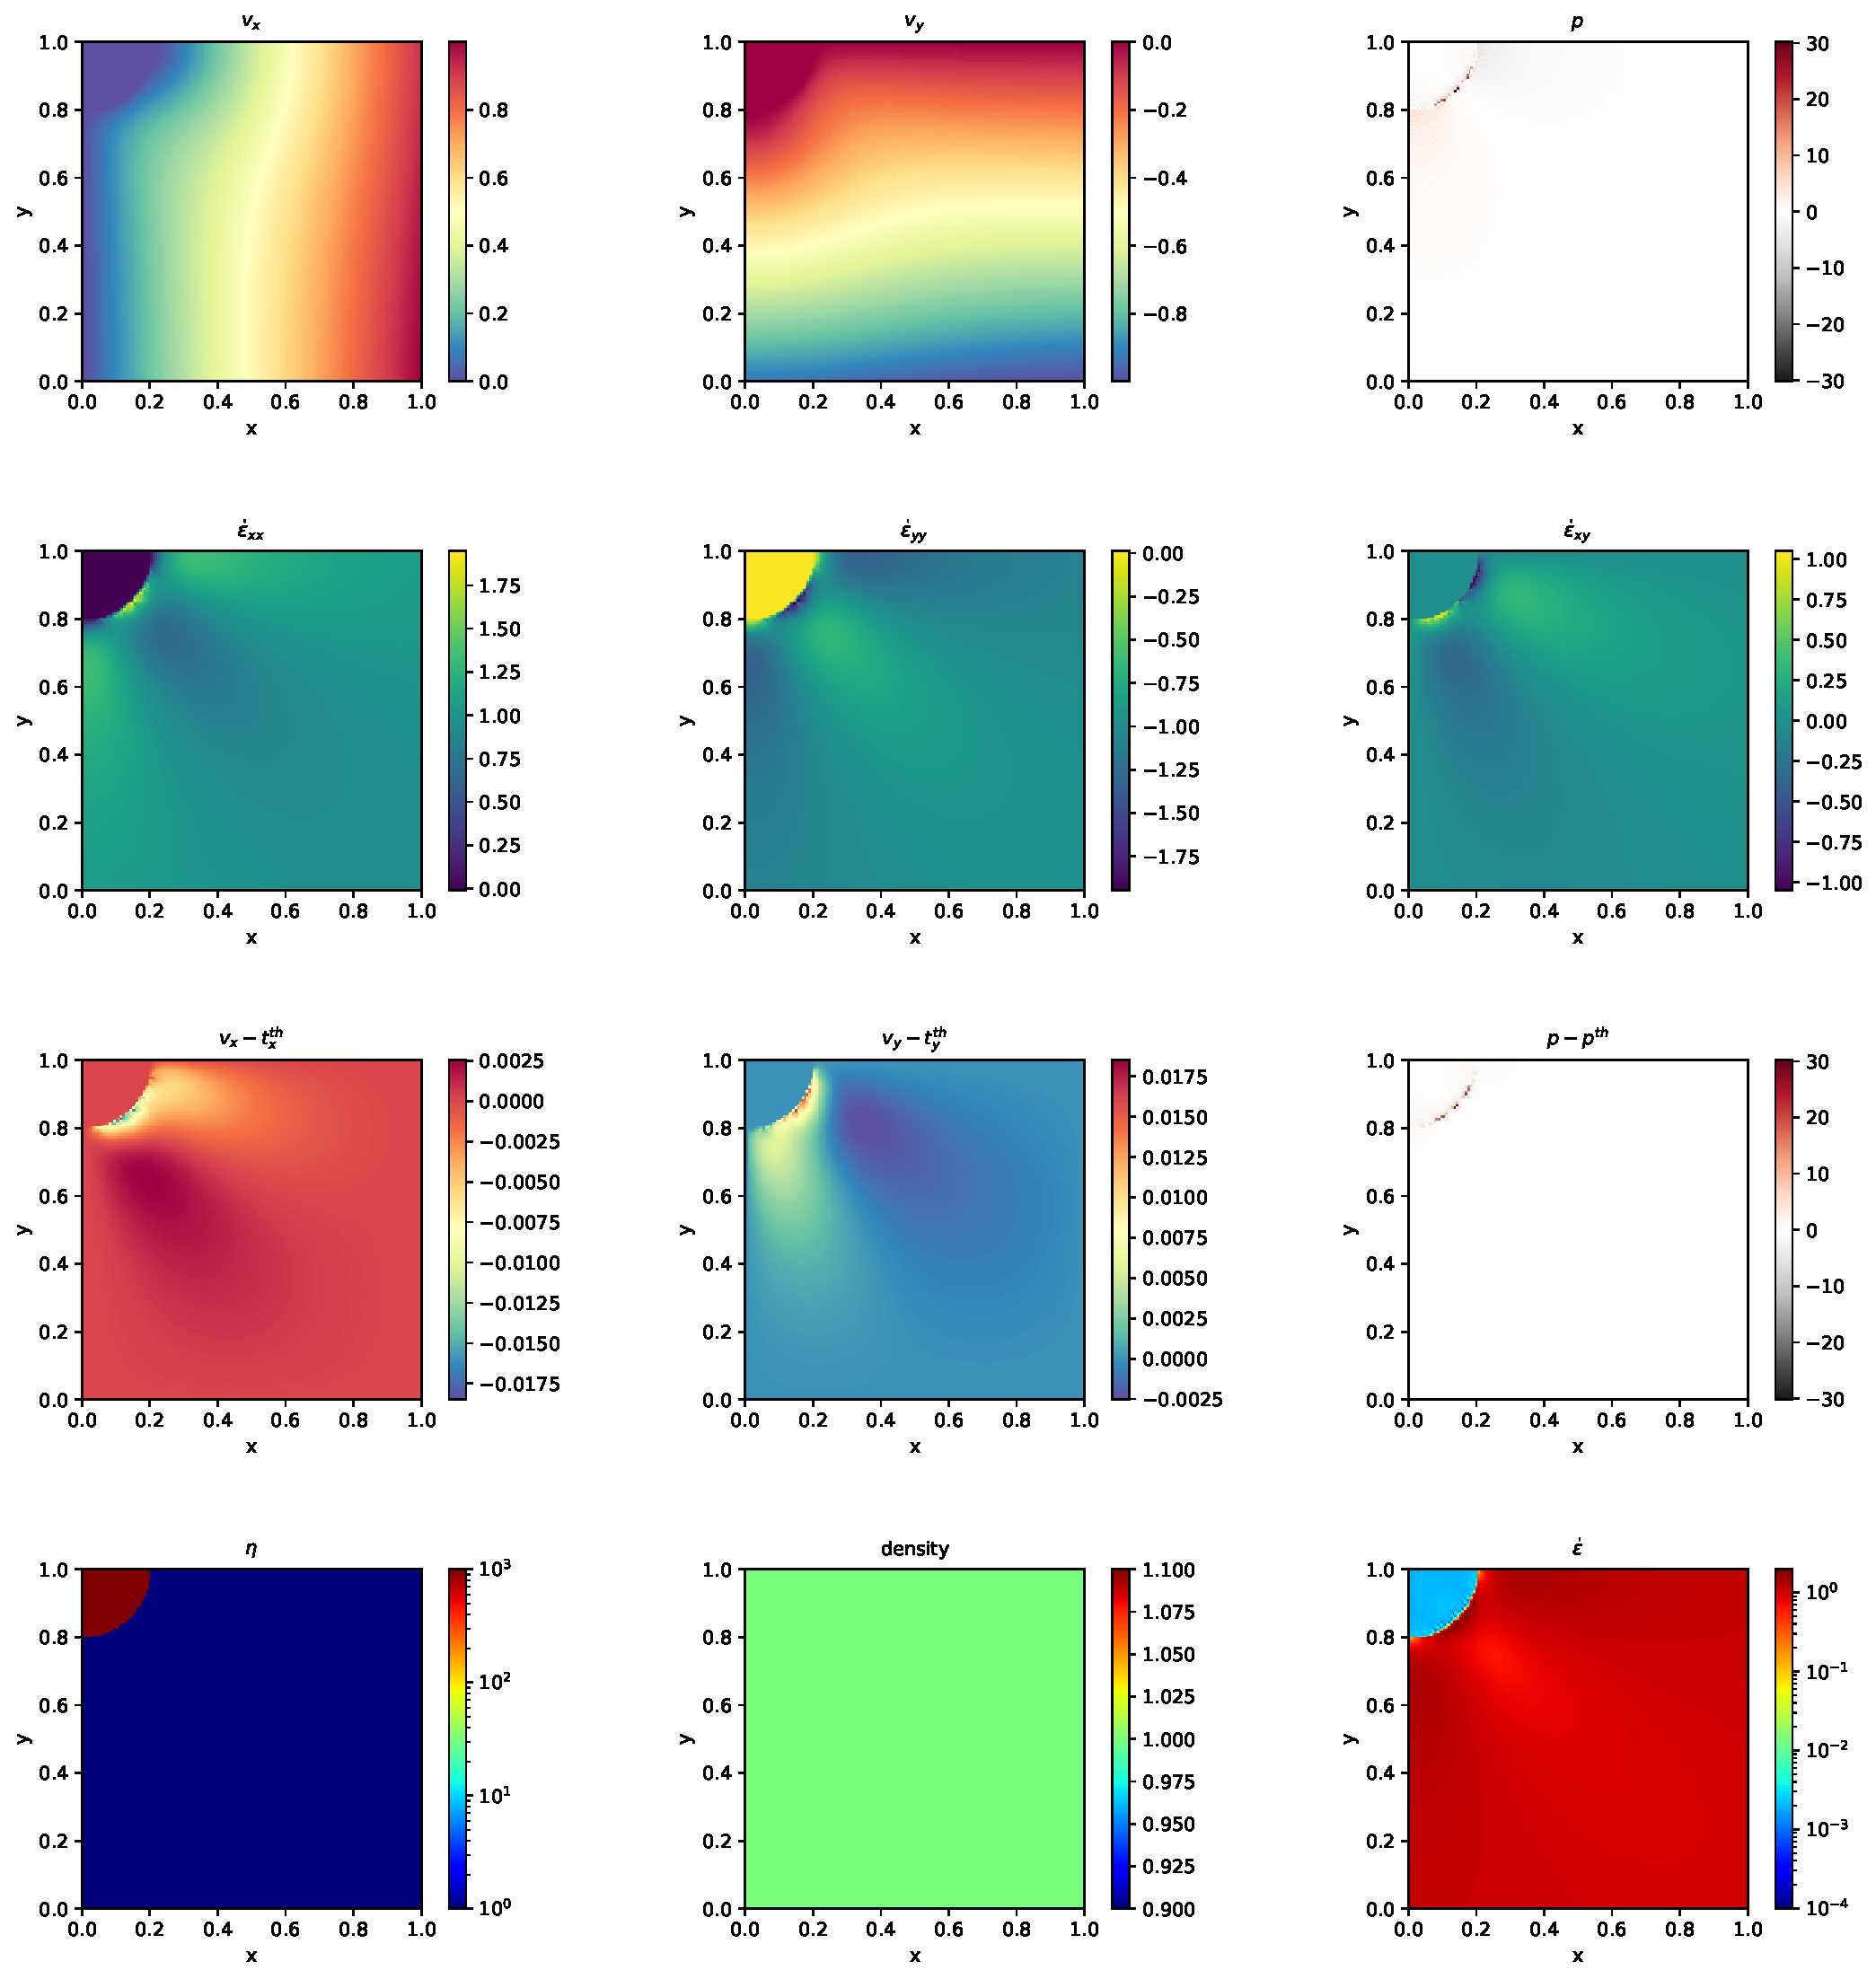
\includegraphics[width=15cm]{python_codes/fieldstone_07/results/solution}

\begin{center}
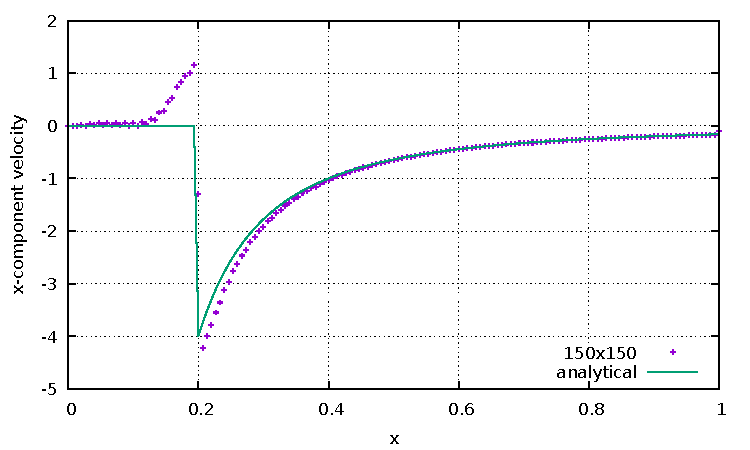
\includegraphics[width=7cm]{python_codes/fieldstone_07/results/pressbottom}
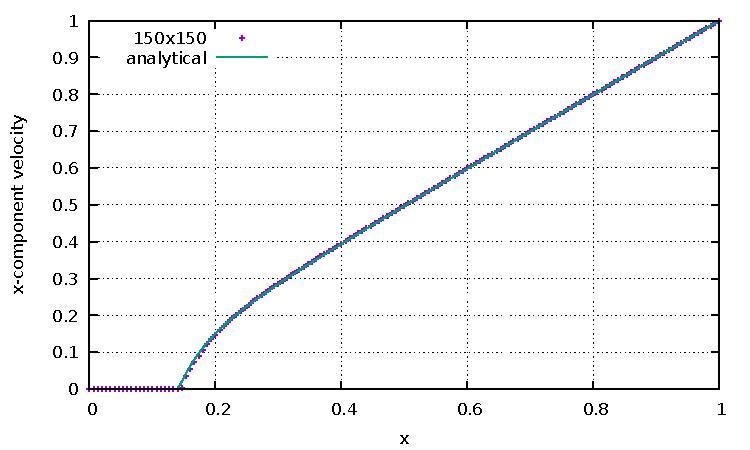
\includegraphics[width=7cm]{python_codes/fieldstone_07/results/veldiag}\\
{\captionfont Left: Pressure at the bottom of the domain. Right: $u$ on the diagonal $x=y$.}
\end{center}

 %%%%%%%%%%%%%%%%%%%%%%%%%%%%%%%%%%%%%%%%%%%%%%%%%

\newpage %%%%%%%%%%%%%%%%%%%%%%%%%%%%%%%%%%%%%%%%%%%%%%%%%%%%%%%%%%%%%%%%%%%%%%%%%%%%%%%%
\section*{
Stone 08: the indentor benchmark 
\label{f08}}
\addcontentsline{toc}{section}{\protect\numberline{} 
Stone 08: the indentor benchmark 
}
\lstinputlisting[language=bash,basicstyle=\small]{python_codes/fieldstone_08/keywords}

\begin{center}
Code at \url{https://github.com/cedrict/fieldstone/tree/master/python_codes/fieldstone_08}
\end{center}

\par\noindent\rule{\textwidth}{0.4pt}
%%%%%%%%%%%%%%%%%%%%%%%%%%%%%%%%%%%%%%%%%%%%%%%%%%%%%%%%%%%%%%%%%%%%%%%%%%%%%%%%%%%%%%%%%

The punch benchmark is one of the few boundary value problems involving plastic solids for which there exists an exact solution. 
Such solutions are usually either for highly simplified geometries (spherical or axial symmetry, for instance) or simplified material models (such as rigid plastic solids) \cite{kacha04}.

In this experiment, a rigid punch indents a rigid plastic half space; the slip line field theory gives 
exact solutions as shown in section~\ref{sec:punch}. 
The plane strain formulation of the equations and the detailed solution to the problem were derived in the Appendix of \cite{thfb08} and are also presented in \cite{gepd98}.

The two dimensional punch problem has been extensively studied numerically for the past 40 years 
\cite{zihl75,zihp95,chpe01,chan99,huhy99,yuti06,bufs08,raab07} and has been used to draw a parallel 
with the tectonics of eastern China in the context of the 
India-Eurasia collision \cite{tamo76,mota77}.
It is also worth noting that it has been carried out in one form or another in series of 
analogue modelling articles 
concerning the same region, with a rigid indenter colliding with a rheologically stratified 
lithosphere \cite{peta88,daco88,jodc90}.
 
Numerically, the one-time step punch experiment is performed on a two-dimensional
domain of purely plastic von Mises material. 
Given that the von Mises rheology yield criterion does not depend on pressure
(see Section~\ref{sec:vMcriterion}), the density of the material and/or the gravity 
vector is set to zero. Sides are set to free slip boundary conditions, the bottom to no slip, 
while a vertical velocity $(0,-v_p)$ is prescribed at the top boundary for nodes 
whose $x$ coordinate is within $[L_x/2-\delta/2,L_x/2+\delta/2]$. 

The following parameters are used: $L_x=1$, $L_y=0.5$, $\mu_{min}=10^{-3}$, 
$\mu_{max}=10^3$, $v_p=1$, $\delta=0.11111$ 
and the yield value of the material is set to $\sigma_Y=1$. 

The analytical solution predicts that the angle of the shear bands stemming from the sides of the punch 
is $\pi/4$, that the pressure right under the punch is $1+\pi$, 
and that the velocity of the rigid blocks on each side of the punch is $v_p/\sqrt{2}$ 
(this is simply explained by invoking conservation of mass).

In what follows I show results of the rough and smooth punch for a 124x68 grid. The difference between the two
lies in the nature of the kinematic boundary conditions under the punched area. 'rough' means that the indentor 
also fixes the horizontal velocity component to zero while it is free in the smooth case.

We see that the smooth punch does not trigger the checkerboard pressure modes as much as the rough case 
and we recover nicely the analytical pressure under the punch \cite{thfb08,gltf18}.

\newpage
%................................................................................
\paragraph{Rough punch} 

\begin{center}
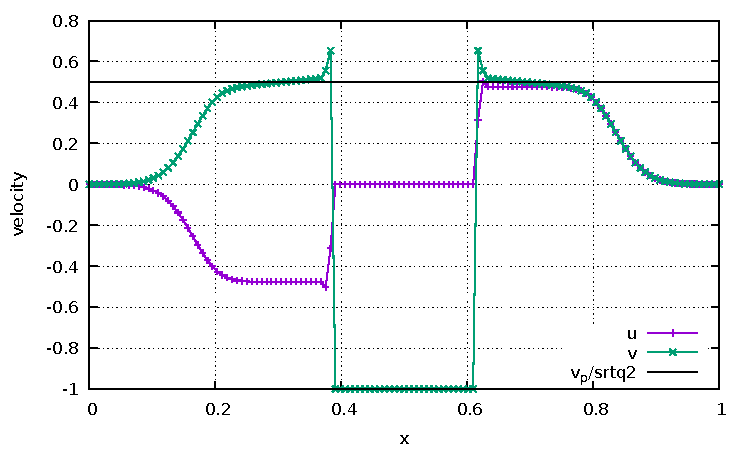
\includegraphics[width=6cm]{python_codes/fieldstone_08/results/rough/velocity.pdf}
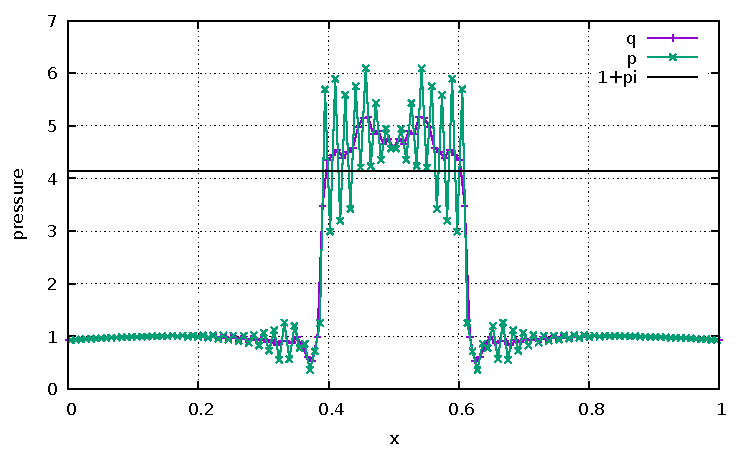
\includegraphics[width=6cm]{python_codes/fieldstone_08/results/rough/pressure.pdf}\\
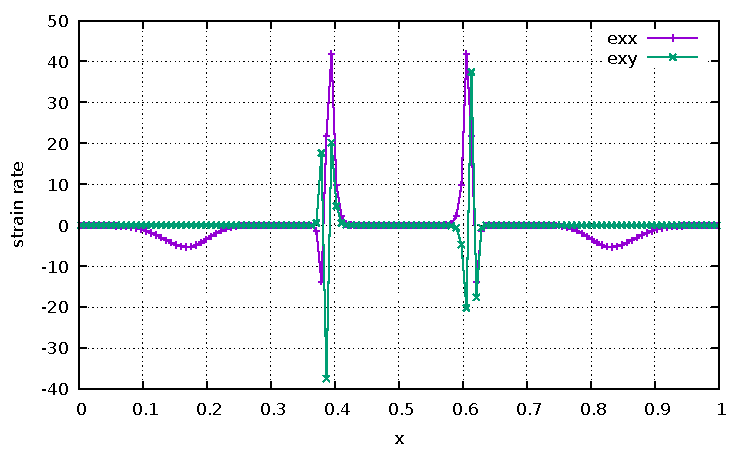
\includegraphics[width=6cm]{python_codes/fieldstone_08/results/rough/strainrate.pdf}
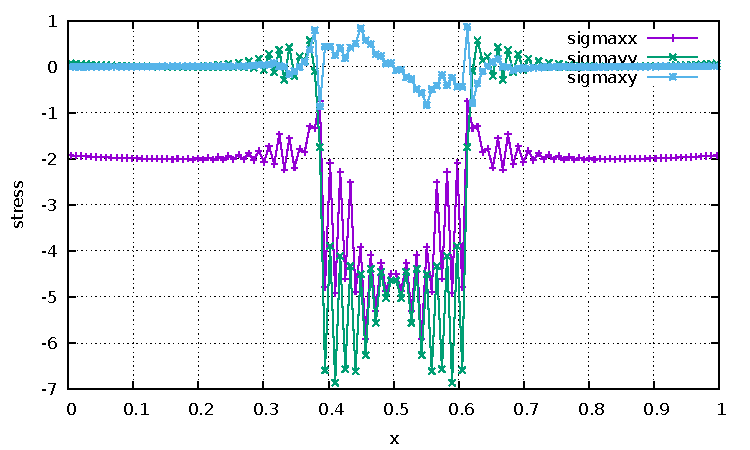
\includegraphics[width=6cm]{python_codes/fieldstone_08/results/rough/stress.pdf}\\
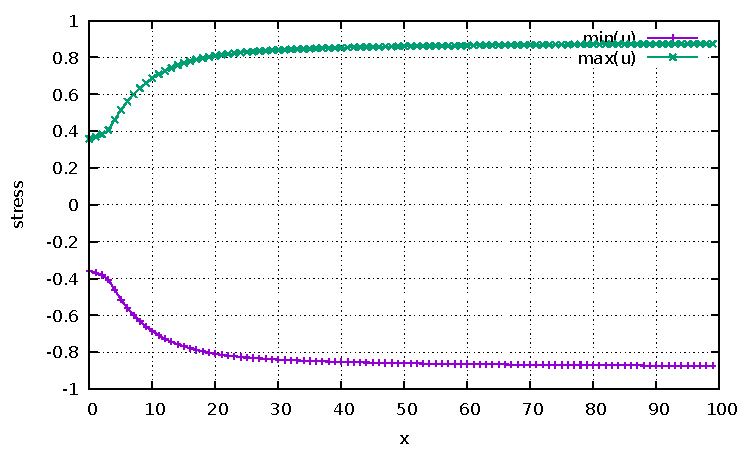
\includegraphics[width=6cm]{python_codes/fieldstone_08/results/rough/u_stats.pdf}
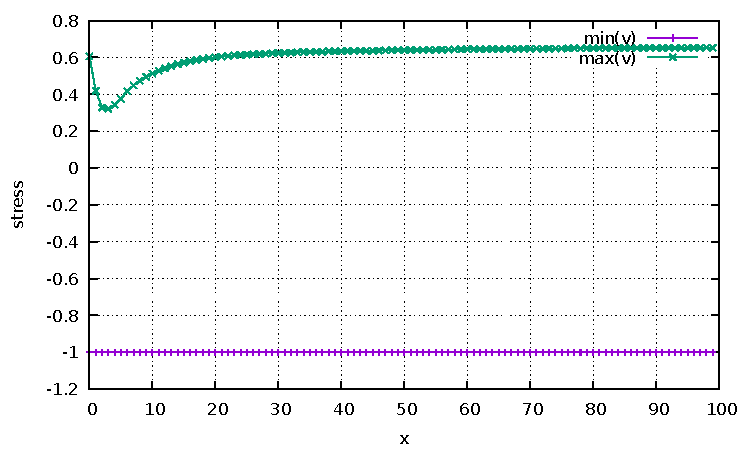
\includegraphics[width=6cm]{python_codes/fieldstone_08/results/rough/v_stats.pdf}\\
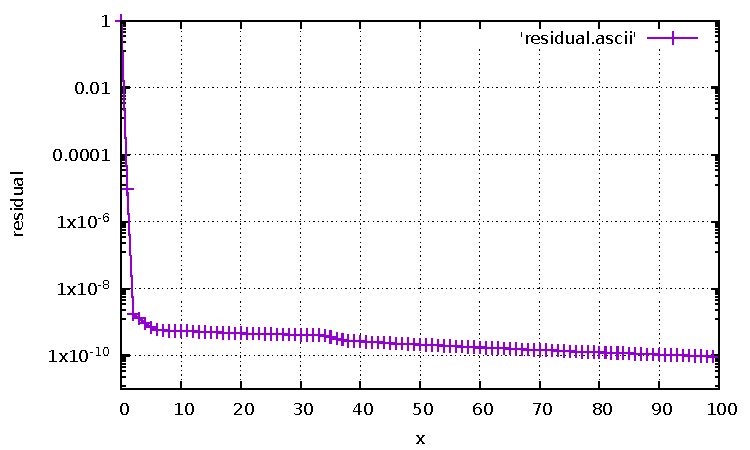
\includegraphics[width=6cm]{python_codes/fieldstone_08/results/rough/residual.pdf}
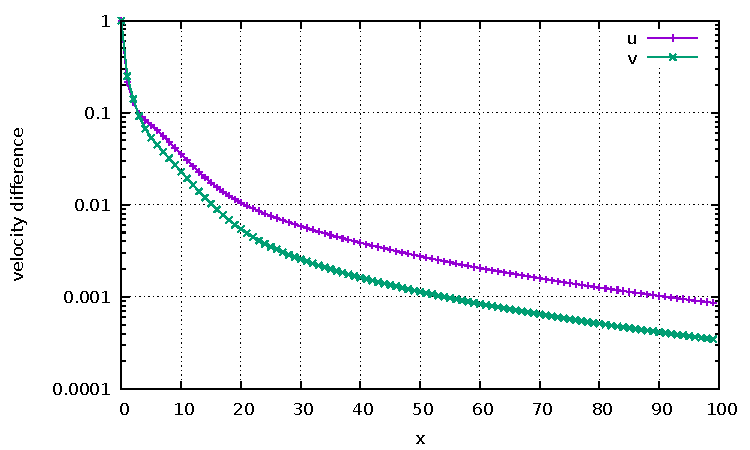
\includegraphics[width=6cm]{python_codes/fieldstone_08/results/rough/diff_uv.pdf}\\
{\captionfont a,b,c,d) velocity, pressure, strainrate and stress at the top of the domain; 
e,f) min/max value of $u$ and $v$;
g,h) residual and normalised velocity difference.}
\end{center}

\newpage
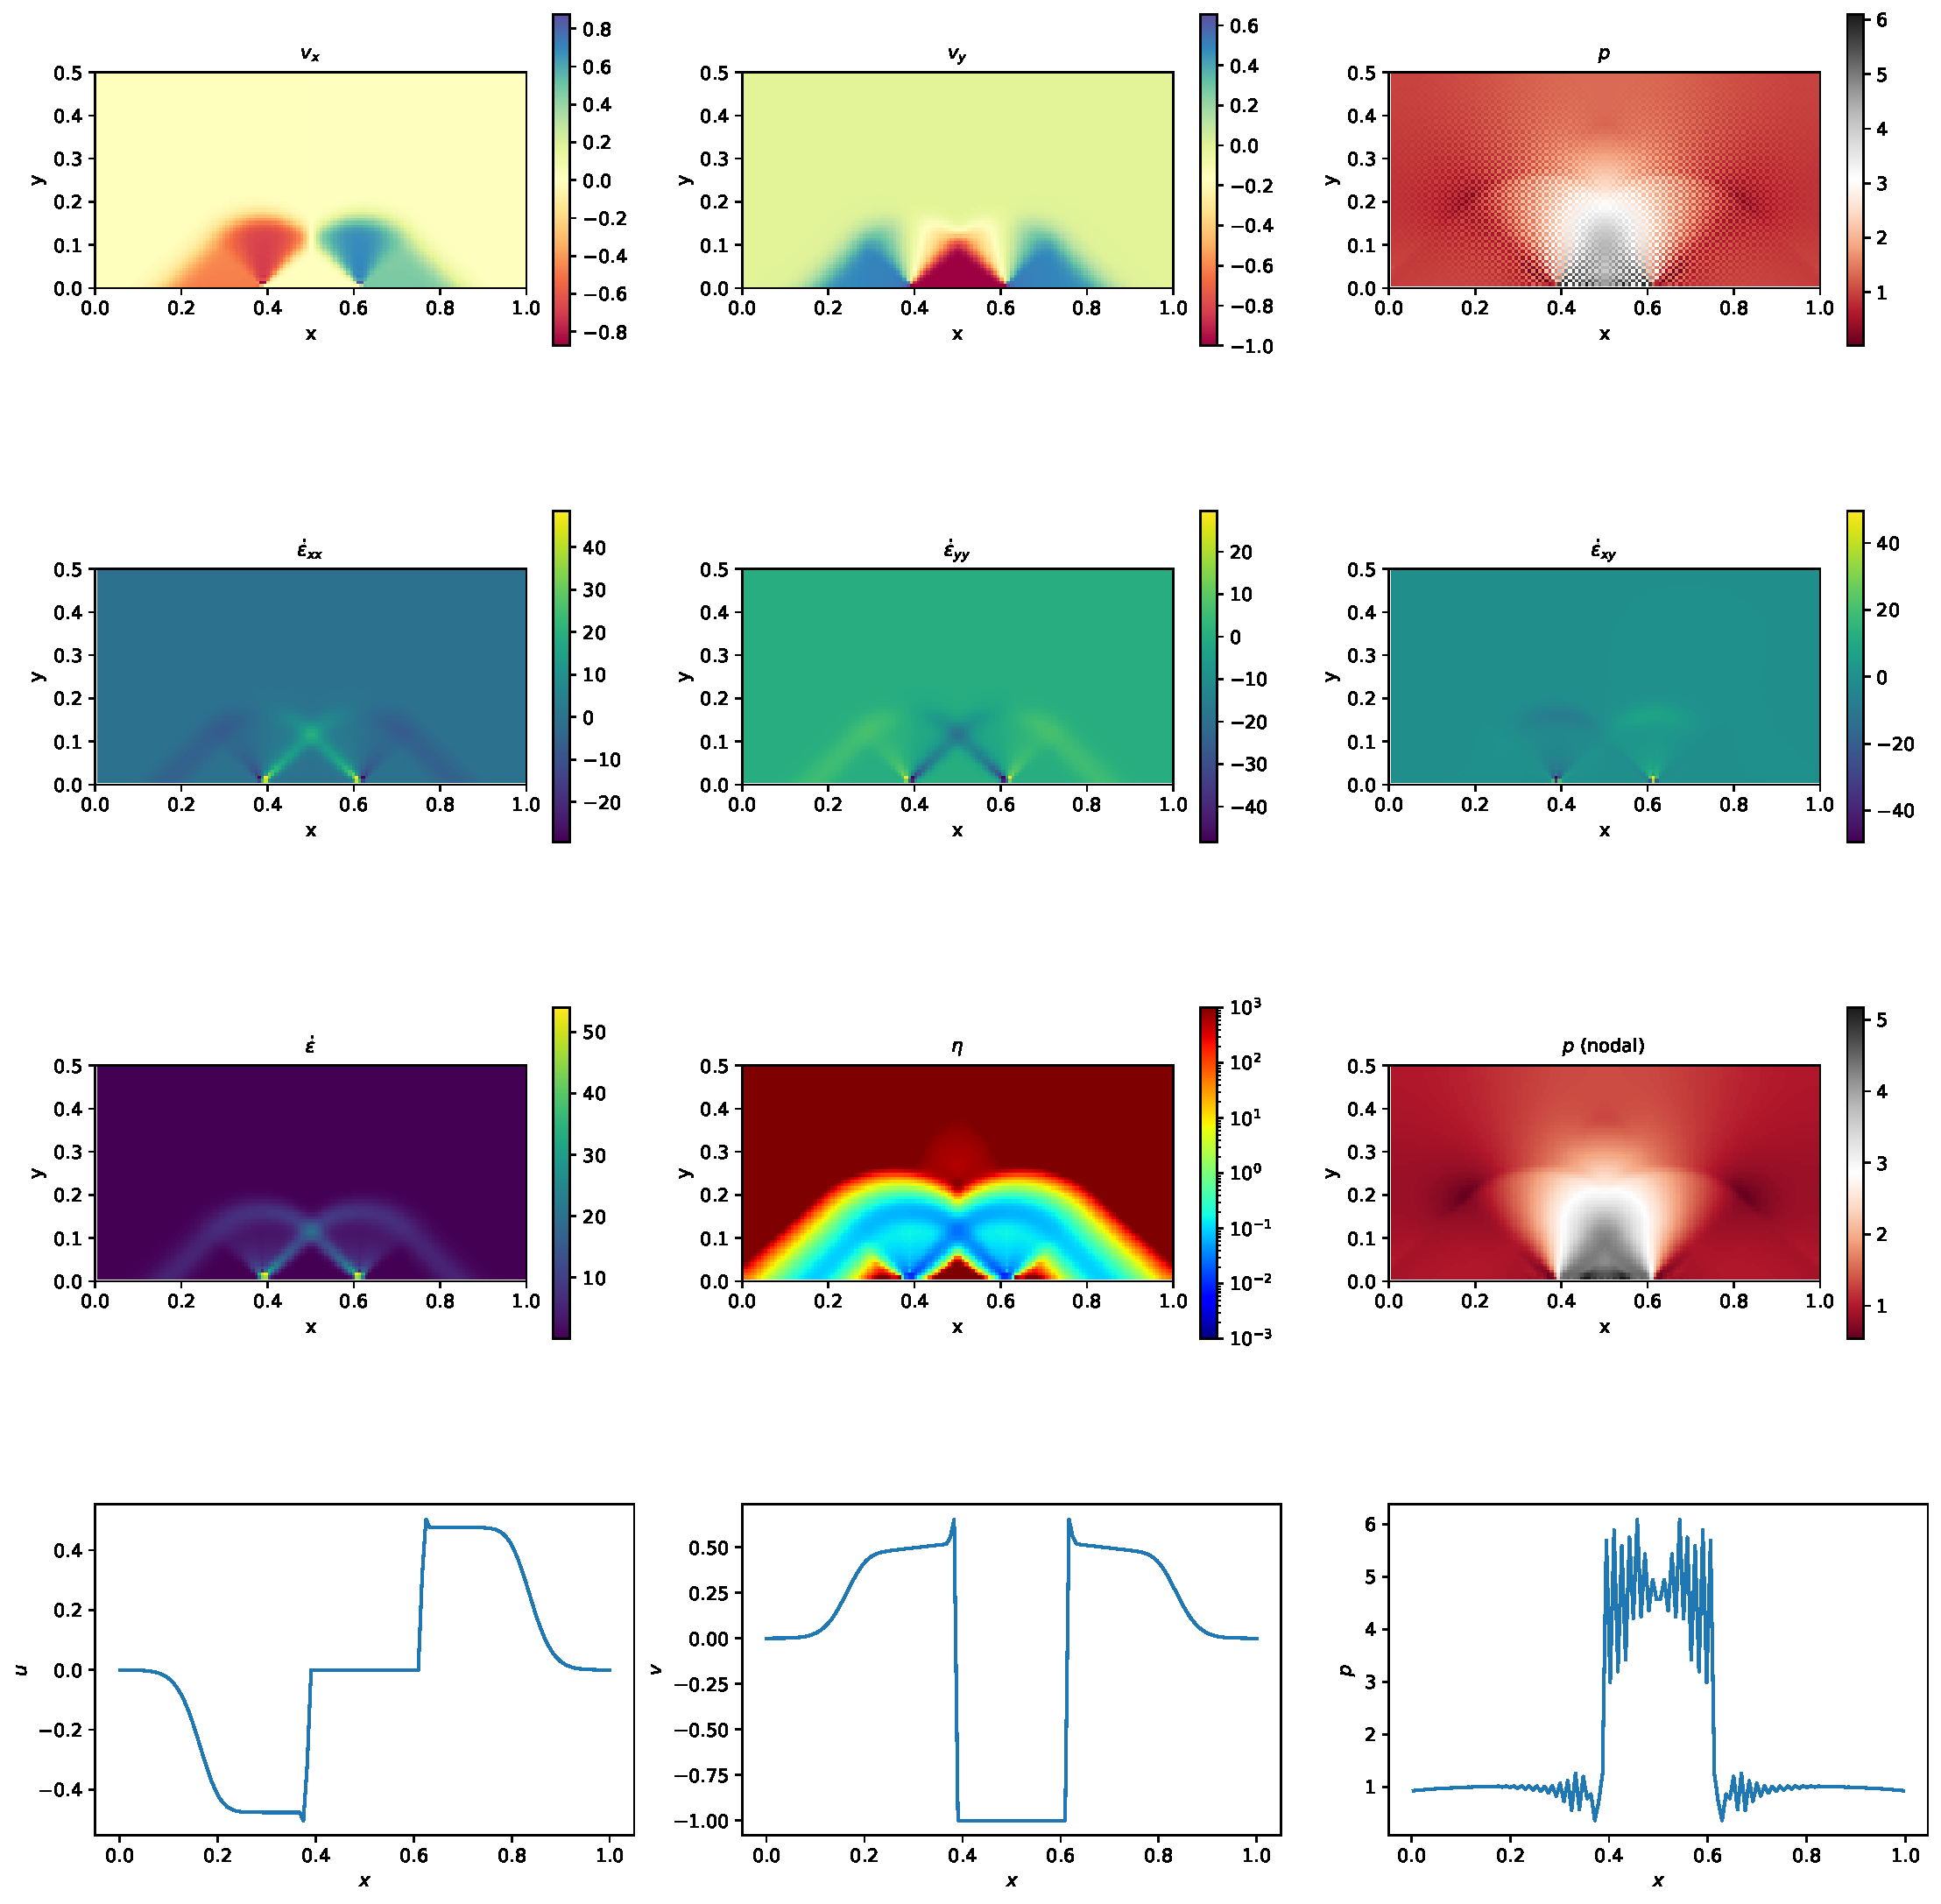
\includegraphics[width=16cm]{python_codes/fieldstone_08/results/rough/solution.pdf}


%................................................................................
\newpage
\paragraph{Smooth punch}

\begin{center}
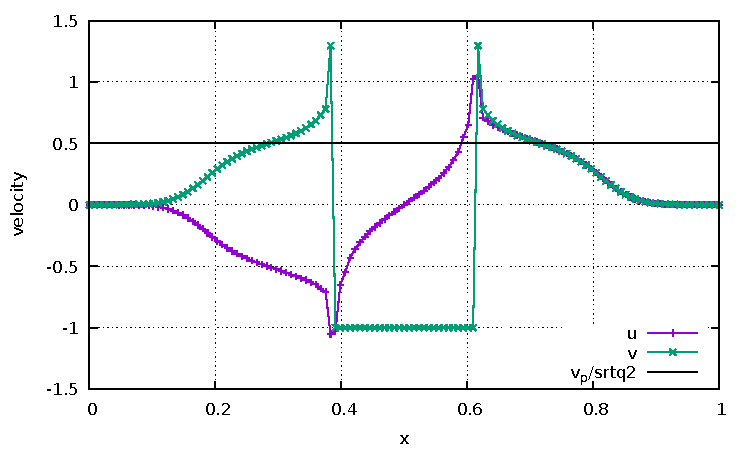
\includegraphics[width=6cm]{python_codes/fieldstone_08/results/smooth/velocity.pdf}
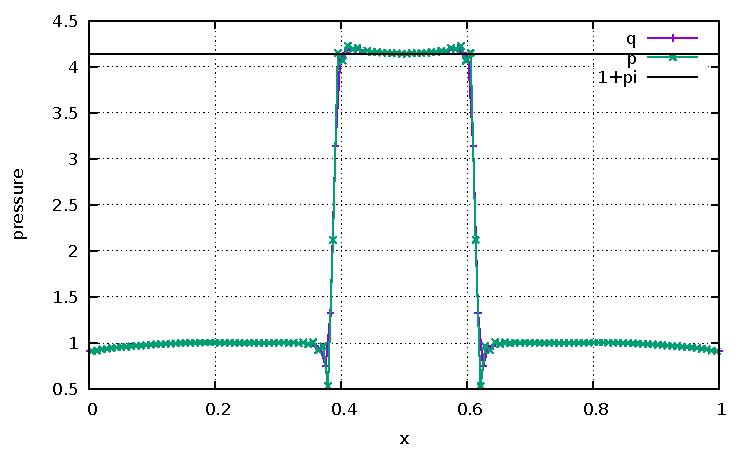
\includegraphics[width=6cm]{python_codes/fieldstone_08/results/smooth/pressure.pdf}\\
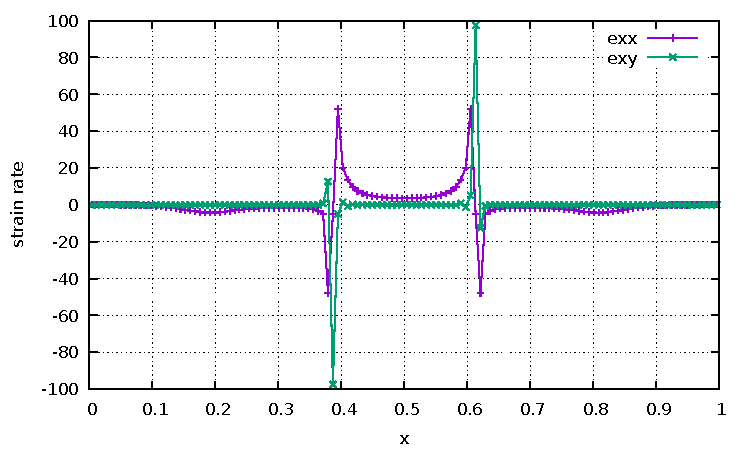
\includegraphics[width=6cm]{python_codes/fieldstone_08/results/smooth/strainrate.pdf}
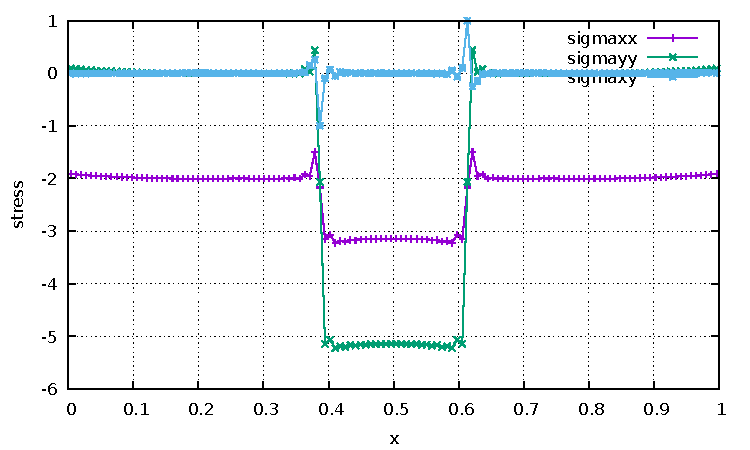
\includegraphics[width=6cm]{python_codes/fieldstone_08/results/smooth/stress.pdf}\\
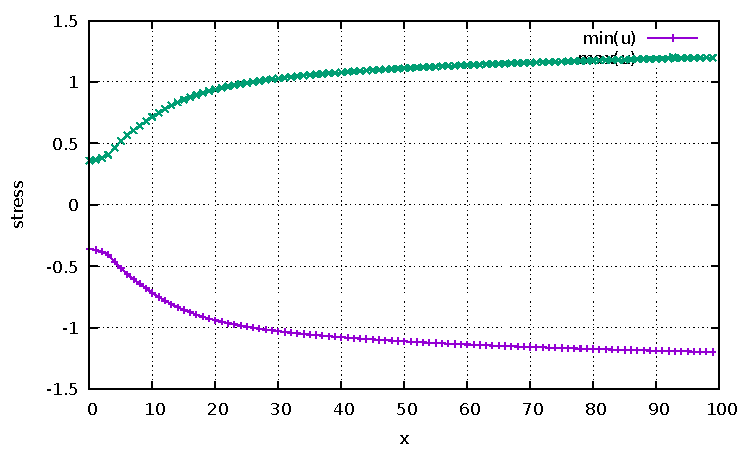
\includegraphics[width=6cm]{python_codes/fieldstone_08/results/smooth/u_stats.pdf}
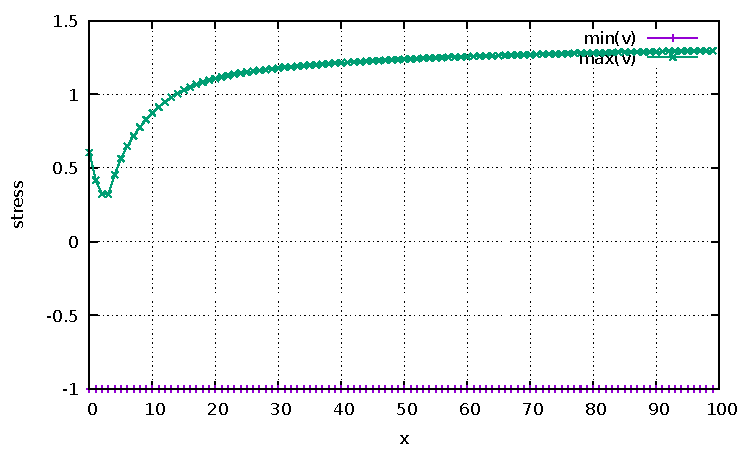
\includegraphics[width=6cm]{python_codes/fieldstone_08/results/smooth/v_stats.pdf}\\
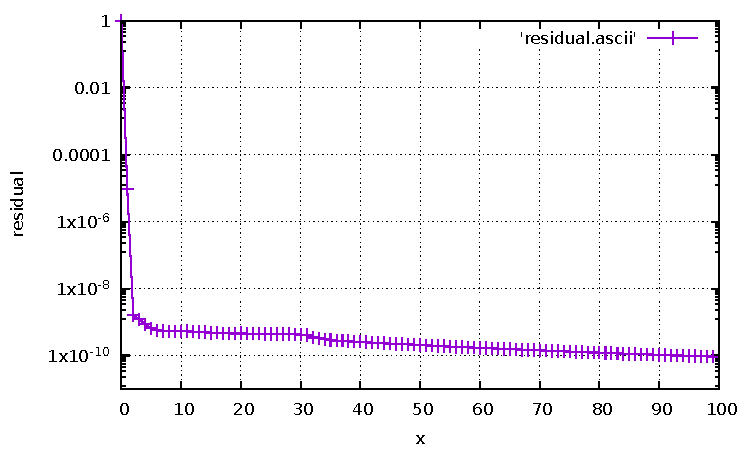
\includegraphics[width=6cm]{python_codes/fieldstone_08/results/smooth/residual.pdf}
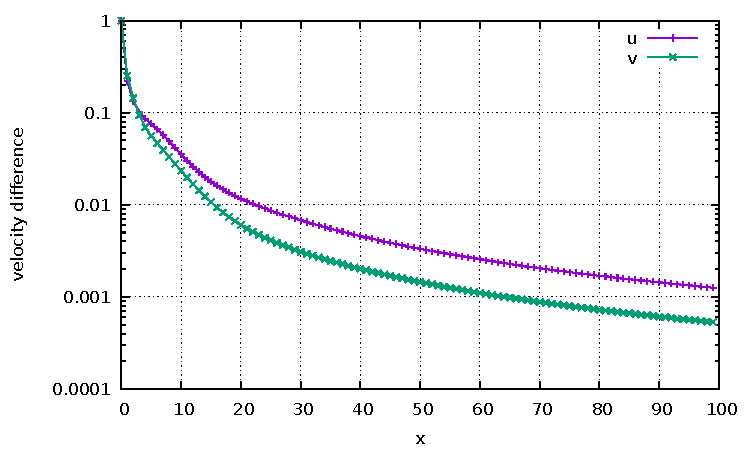
\includegraphics[width=6cm]{python_codes/fieldstone_08/results/smooth/diff_uv.pdf}\\
{\captionfont a,b,c,d) velocity, pressure, strainrate and stress at the top of the domain; 
e,f) min/max value of $u$ and $v$;
g,h) residual and normalised velocity difference.}
\end{center}

\newpage
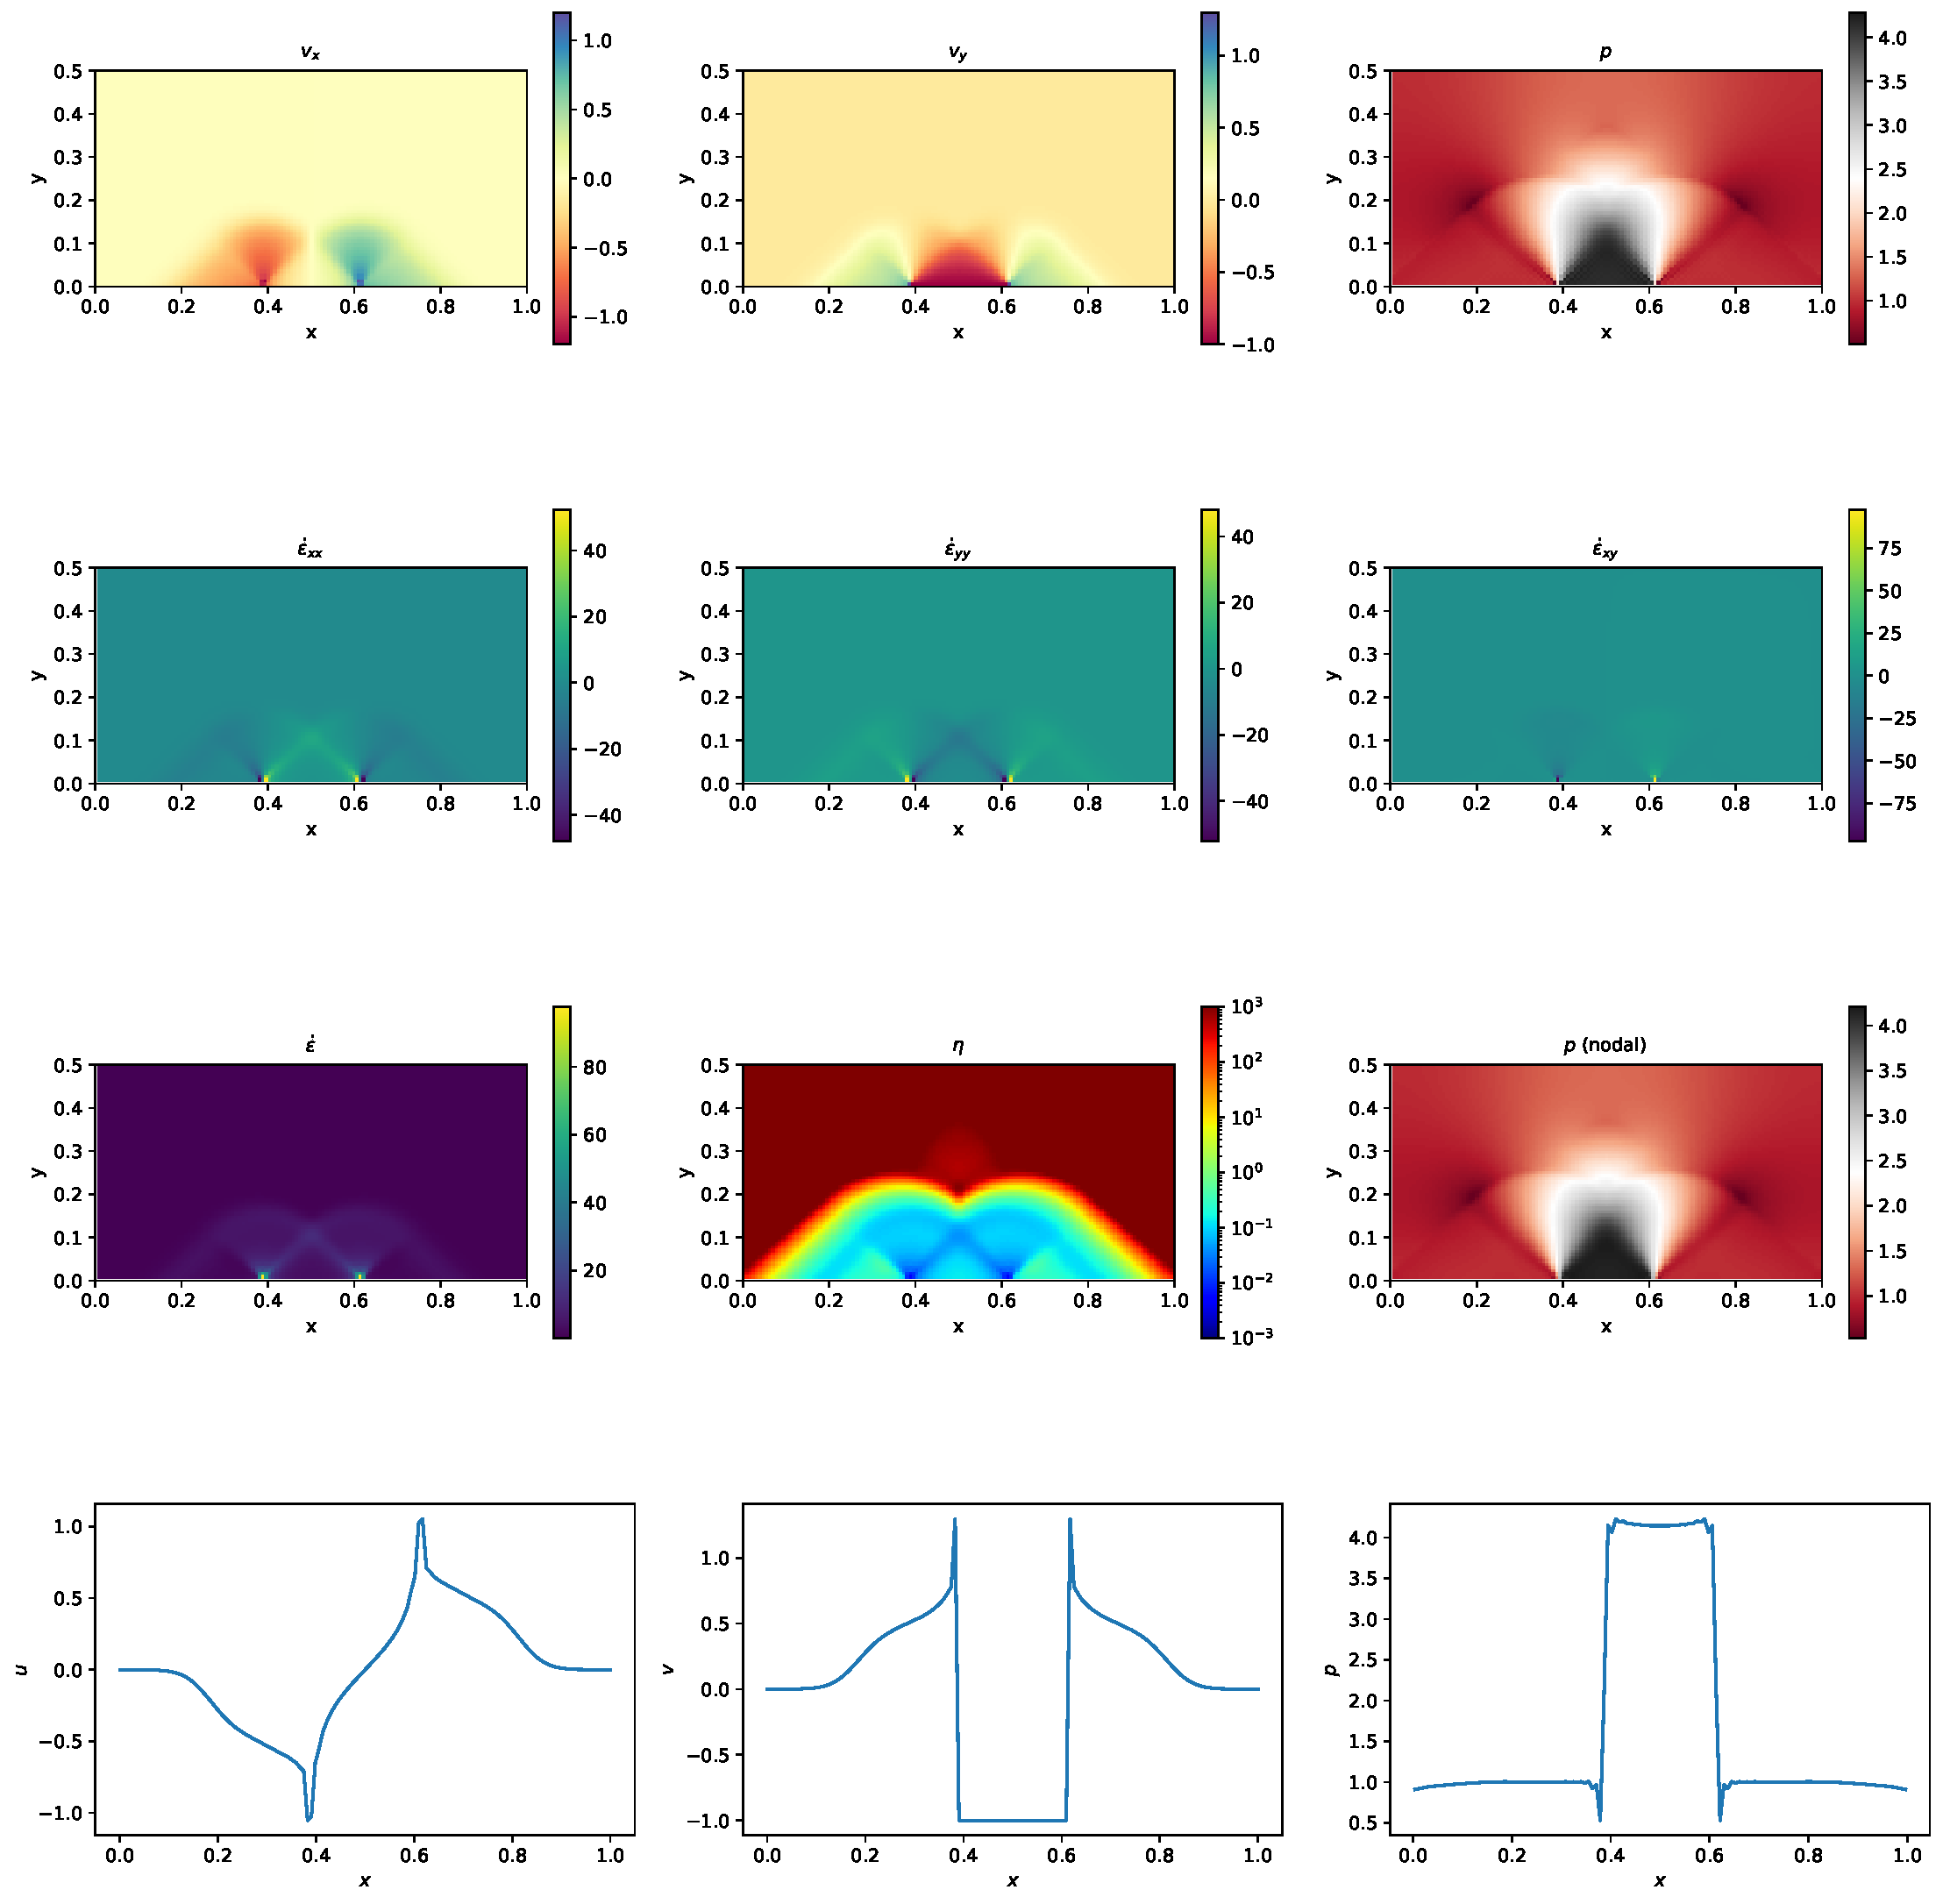
\includegraphics[width=16cm]{python_codes/fieldstone_08/results/smooth/solution.pdf}




 %%%%%%%%%%%%%%%%%%%%%%%%%%%%%%%%%%%%%%%%%%%%%%%%%

\newpage %%%%%%%%%%%%%%%%%%%%%%%%%%%%%%%%%%%%%%%%%%%%%%%%%%%%%%%%%%%%%%%%%%%%%%%%%%%%%%%%
\section*{
Stone 09: the annulus benchmark with $Q_1\times P_0$ elements
\label{f09}}
\addcontentsline{toc}{section}{\protect\numberline{} 
Stone 09: the annulus benchmark with $Q_1\times P_0$ elements
}

{\sl This fieldstone was developed in collaboration with Prof. E.G.P. Puckett}. 
\index{contributors}{E.G.P. Puckett}

An analytical solution to the
isoviscous incompressible Stokes equations is derived in an annulus geometry.
The velocity and pressure fields are as follows:

\begin{eqnarray}
v_r(r,\theta)     &=&  g(r) k \sin(k\theta), \\
v_\theta(r,\theta)&=&  f(r) \cos(k \theta), \\ 
p(r,\theta)       &=&  k h(r) \sin(k \theta), \\
\rho (r,\theta)   &=& \aleph(r) k \sin (k \theta), 
\end{eqnarray}
with
\begin{eqnarray}
f(r)&=&Ar+B/r, \\
g(r) &=& \frac{A}{2}r  +  \frac{B}{r} \ln r + \frac{C}{r}, \\
h(r)&=& \frac{2g(r)-f(r)}{r},  \\
\aleph(r) &=& g'' - \frac{g'}{r}  - \frac{g}{r^2} (k^2 - 1)  + \frac{f}{r^2}   + \frac{f'}{r}, \\
A &=& -C\frac{2(\ln R_1 - \ln R_2)} { R_2^2 \ln R_1  - R_1^2 \ln R_2}, \\
B &=& -C \frac{R_2^2-R_1^2}{R_2^2 \ln R_1 - R_1^2 \ln R_2}.
\end{eqnarray}

The parameters $A$ and $B$ are chosen so that $v_r(R_1)=v_r(R_2)=0$, i.e.
the velocity is tangential to both inner and outer surfaces.
The gravity vector is radial and of unit length.
In the present case, we set $R_1=1$, $R_2=2$ and $C=-1$. 

\begin{center}
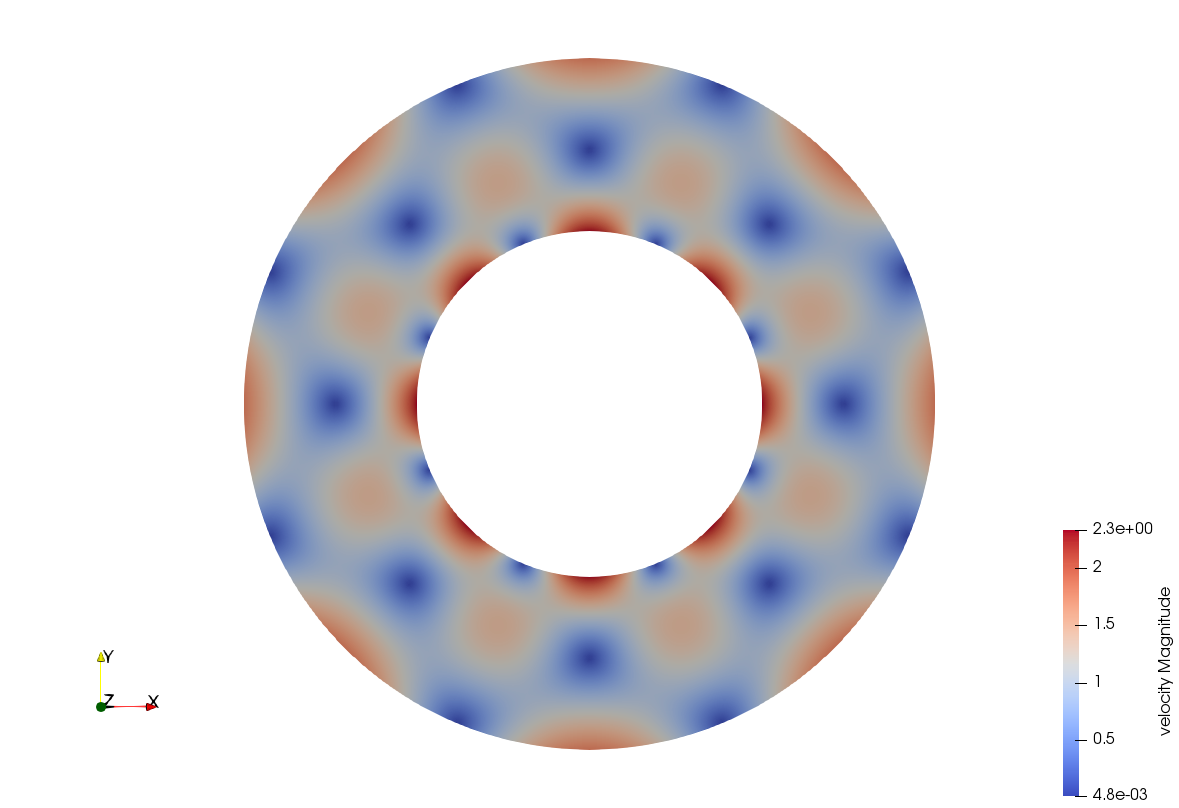
\includegraphics[width=5cm]{python_codes/fieldstone_09/velocity}
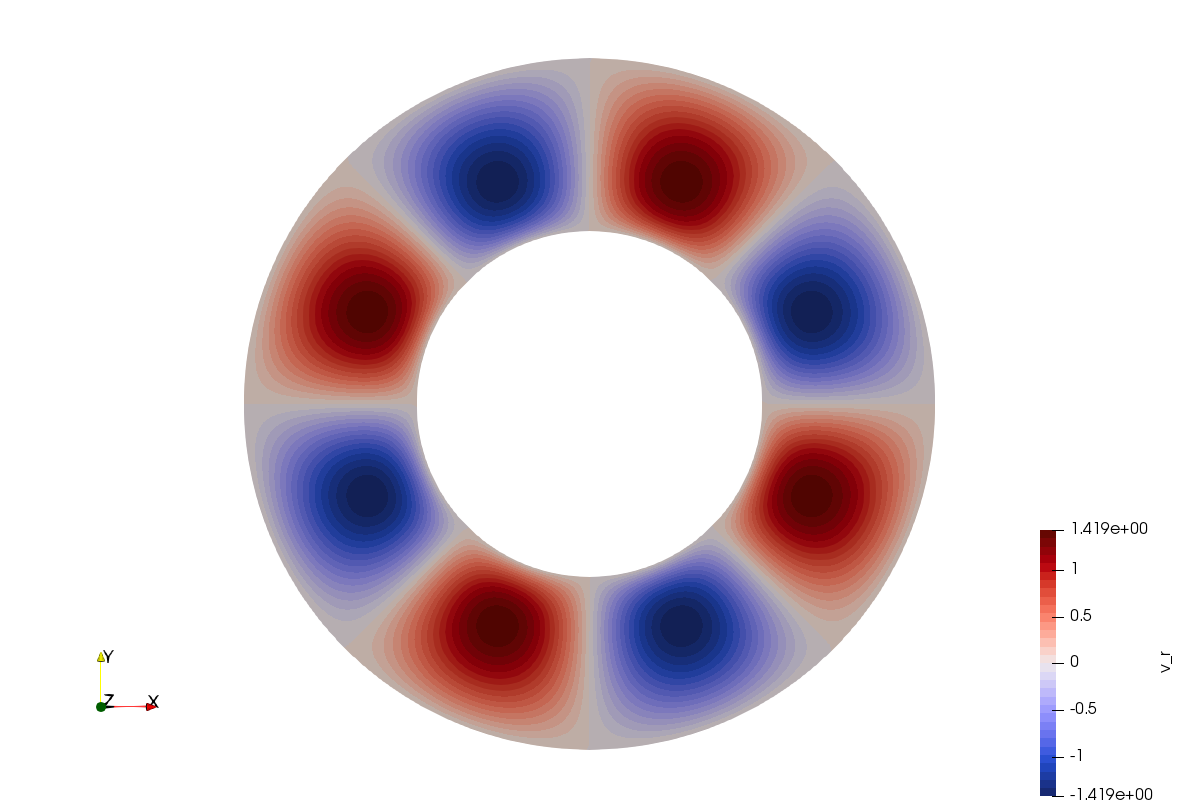
\includegraphics[width=5cm]{python_codes/fieldstone_09/vr}
\includegraphics[width=5cm]{python_codes/fieldstone_09/vtheta}\\
{\small Left to right: velocity norm, $r$ component, $\theta$ component}
\end{center}

\begin{center}
\includegraphics[width=7cm]{python_codes/fieldstone_09/density}
\includegraphics[width=7cm]{python_codes/fieldstone_09/pressure}\\
{\small Left: density field; right: pressure field.}
\end{center}

\begin{center}
\includegraphics[width=7cm]{python_codes/fieldstone_09/psi}
\includegraphics[width=7cm]{python_codes/fieldstone_09/psi_arrows}\\
{\small Left: $\psi$ field; right: $\psi$ isolines with velocity arrows.}
\end{center}

\includegraphics[width=15cm]{python_codes/fieldstone_09/errors}

 %%%%%%%%%%%%%%%%%%%%%%%%%%%%%%%%%%%%%%%%%%%%%%%%%

\newpage %%%%%%%%%%%%%%%%%%%%%%%%%%%%%%%%%%%%%%%%%%%%%%%%%%%%%%%%%%%%%%%%%%%%%%%%%%%%%%%%
\section*{
Stone 10: Stokes sphere (3D) - penalty 
\label{f10}}
\addcontentsline{toc}{section}{\protect\numberline{} 
Stone 10: Stokes sphere (3D) - penalty 
}
\lstinputlisting[language=bash,basicstyle=\small]{python_codes/fieldstone_10/keywords}

\begin{center}
Code at \url{https://github.com/cedrict/fieldstone/tree/master/python_codes/fieldstone_10}
\end{center}

\par\noindent\rule{\textwidth}{0.4pt}
%%%%%%%%%%%%%%%%%%%%%%%%%%%%%%%%%%%%%%%%%%%%%%%%%%%%%%%%%%%%%%%%%%%%%%%%%%%%%%%%%%%%%%%%%%%%

The domain is a unit cube. Free slip boundary conditions 
are imposed on all sides. The mesh counts 
nelx*nely*nelz=nel elements and 
nnx*nny*nnz=NV nodes.
The density and the viscosity are prescribed in the domain 
by means of two functions:
the density is set to 2 inside a sphere of radius 0.123 centered 
at (0.5,0.5,0.5) and 1 outside. The viscosity is 100 inside the sphere
and 1 outside.  The gravity vector is set to $\vec{g}=(0,0,-1)$.

The FE matrix size grows even faster now than in the previous 2D case so
choosing the right matrix storage is of paramount importance. 

Three experiments are carried out:
\begin{enumerate}
\item the one described above.
We see that the pressure field is dominated by the lithostatic signal.
\item same as experiment 1, but a reference density of 1 is substracted to all densities, so that 
the sphere density is 1 and the density of the surrounding fluid is now 0. In essence, we remove a
'background' density which does not participate in the flow generation, and thereby get rid of the 
lithostatic signal of the pressure.
\item same as experiment 2, but the top boundary is now open (free surface)
\end{enumerate} 


\begin{center}
\includegraphics[width=5cm]{python_codes/fieldstone_10/results/grid}
\includegraphics[width=5cm]{python_codes/fieldstone_10/results/vel}
\includegraphics[width=5cm]{python_codes/fieldstone_10/results/press}\\
\includegraphics[width=5cm]{python_codes/fieldstone_10/results/visc}
\includegraphics[width=5cm]{python_codes/fieldstone_10/results/dens}\\
{\small Experiment 1: resolution 24x24x24}
\end{center}

\begin{center}
\includegraphics[width=5cm]{python_codes/fieldstone_10/results/dens_2}
\includegraphics[width=5cm]{python_codes/fieldstone_10/results/press_2}\\
{\small Experiment 2: Density and pressure fields. Resolution 24x24x24}
\end{center}


\begin{center}
\includegraphics[width=5cm]{python_codes/fieldstone_10/results/press_3}
\includegraphics[width=5cm]{python_codes/fieldstone_10/results/vel_3}\\
{\small Experiment 3: pressure and velocity fields. Resolution 24x24x24}
\end{center}

\begin{center}
\includegraphics[width=5cm]{python_codes/fieldstone_10/results/model1/pressure.pdf}
\includegraphics[width=5cm]{python_codes/fieldstone_10/results/model2/pressure.pdf}
\includegraphics[width=5cm]{python_codes/fieldstone_10/results/model3/pressure.pdf}\\
{\captionfont Elemental pressure for all elements as a function of their vertical (middle) coordinate for
(from left to right) experiments 1, 2 and 3. }
\end{center}

Note that a similar fortran code is present in the folder. 
 %%%%%%%%%%%%%%%%%%%%%%%%%%%%%%%%%%%%%%%%%%%%%%%%%

\newpage %%%%%%%%%%%%%%%%%%%%%%%%%%%%%%%%%%%%%%%%%%%%%%%%%%%%%%%%%%%%%%%%%%%%%%%%%%%%%%%%
\section*{
Stone 11: stokes sphere (3D) - mixed formulation 
\label{f11}}
\addcontentsline{toc}{section}{\protect\numberline{} 
Stone 11: stokes sphere (3D) - mixed formulation 
}
\lstinputlisting[language=bash,basicstyle=\small]{python_codes/fieldstone_11/keywords}

The setup is identical to the one of the \stone~10.

The difference lies in how we solve the Stokes equation. This stone does not rely on 
the penalty method (Section \ref{sec:penalty}) 
but instead used a mixed formulation, i.e. we solve for both 
velocity and pressure at the same time (see Section~\ref{sec:mixed}).

In the case when free slip boundary conditions are applied on all 
6 faces of the cube we know that there is a pressure nullspace, i.e.
that the pressure can only be computed up to a constant. In order to 
remove this nullspace one must add an additional constraint 
We here choose to (somewhat arbitrarily) enforce that the average pressure 
over the whole domain is zero:
\[
<p>=\frac{1}{|\Omega|} \int_\Omega p \; dV =0 
\]
Since the code relies of discontinuous zero-th order polynomial shape functions 
for pressure this condition simply writes (and since $|\Omega|=1$):
\[
<p>=\frac{1}{|\Omega|} \int_\Omega p\;  dV 
=  \sum_{e} \int_{\Omega_e} p dV = \sum_e p_e V_e = h^3 \sum_e p_e =0
\]
Dividing all by $h^3$, the condition becomes simply:
\[
p_1 + p_2 + p_3 + ... + p_{nel} = 0
\]
How this constraint is incorporated in the Stokes matrix is explained in Section~\ref{ss_pnorm}.

It is also important to remember that if one now switches to a free surface at the top then 
the null space is absent from the equations and the constraint should be removed/switched off.

The pressure normalisation is controled by the boolean {\sl pnormalise} in the code. 
Since the pressure constraint adds a line to the global FE, we then logically have:
\begin{lstlisting}
if pnormalise:
   a_mat = np.zeros((Nfem+1,Nfem+1),dtype=np.float64) 
   rhs   = np.zeros(Nfem+1,dtype=np.float64)    
else:
   a_mat = np.zeros((Nfem,Nfem),dtype=np.float64)
   rhs   = np.zeros(Nfem,dtype=np.float64)       
\end{lstlisting} 
Once the solve has been done, we retrieve the separate velocity and pressure fields as follows:
\begin{lstlisting}
u,v,w=np.reshape(sol[0:NfemV],(nnp,3)).T
p=sol[NfemV:Nfem]
\end{lstlisting} 
and the Lagrange multiplier is a scalar at the bottom of the array:
\begin{lstlisting}
if pnormalise:
   print("     -> Lagrange multiplier: %.4es" % sol[Nfem])
\end{lstlisting} 

It is quite easy in python to visualise the matrix structure 
with the spy function:
\begin{lstlisting}
plt.spy(a_mat)
\end{lstlisting} 
and we see that we indeed recover
the block structure with a zero block for the pressure-pressure entries.  
\begin{center}
\includegraphics[width=7cm]{python_codes/fieldstone_11/results/matrix6x6x6.pdf}
\includegraphics[width=7cm]{python_codes/fieldstone_11/results/matrix16x16x16.pdf}\\
{\captionfont Sparsity pattern of the Stokes matrix for a 6x6x6 mesh (left) and a 16x16x16 mesh (right).}
\end{center}

\begin{center}
\includegraphics[width=7cm]{python_codes/fieldstone_11/results/vel}
\includegraphics[width=7cm]{python_codes/fieldstone_11/results/press}
\includegraphics[width=8cm]{python_codes/fieldstone_11/results/sr}\\
{\captionfont Velocity, pressure and effective strain rate fields for a 20x20x20 mesh.}
\end{center}
 %%%%%%%%%%%%%%%%%%%%%%%%%%%%%%%%%%%%%%%%%%%%%%%%%

\newpage %%%%%%%%%%%%%%%%%%%%%%%%%%%%%%%%%%%%%%%%%%%%%%%%%%%%%%%%%%%%%%%%%%%%%%%%%%%%%%%%
\section*{
Stone 12: consistent pressure recovery 
\label{f12}}
\addcontentsline{toc}{section}{\protect\numberline{} 
Stone 12: consistent pressure recovery 
}
\lstinputlisting[language=bash,basicstyle=\small]{python_codes/fieldstone_12/keywords}

\begin{center}
Code at \url{https://github.com/cedrict/fieldstone/tree/master/python_codes/fieldstone_12}
\end{center}

\par\noindent\rule{\textwidth}{0.4pt}
%%%%%%%%%%%%%%%%%%%%%%%%%%%%%%%%%%%%%%%%%%%%%%%%%%%%%%%%%%%%%%%%%%%%%%%%%%%%%%%%%%%%%%%%%%%%%%


We start from the analytical benchmark of Section \ref{mms1} and we use $Q_1 \times P_0$
elements with a penalty formulation. 
We have seen in stone $\# 1$ how to recover the elemental pressure as a postprocessing step. 
However, the discontinous nature of the pressure field (and the presence of a
parasitic checkerboard mode) can be problematic for many reasons 
(pressure enters the rheology, equation of state, plotting, ...). 
We then wish to project the elemental pressure onto the nodes of the mesh while at the same 
time filtering the checkerboard mode out. 

Terminology: in general, when a discontinuous elemental pressure is used in a stone, 
it is called $p$ while its projection onto the nodes is coined $q$. 
In this case we compute several nodal pressures as explained in Section~\ref{psmoothing}:

\begin{itemize}
%...........
\item $q_1$: smoothed pressure obtained with the  center-to-node approach (scheme 1)

\item $q_2$: the nodal pressure obtained by smoothing the elemental pressure using element areas (scheme 2)

\item $q_3$: the nodal pressure obtained by smoothing the elemental p using triangle areas (scheme 3)

\item $q_4$: smoothed pressure obtained with the center-to-node approach with inverse element area weighing.

\item $q_5$: is not computed because same as 6.

\item $q_6$: consistent pressure recovery through FE (scheme 5 \& 6)

\item $q_7$: consistent pressure recovery with lumped mass matrix. 

\item $q_8$: bilinear interpolation. 

\end{itemize}

Since the setups showcase Dirichlet boundary conditions on all four sides, 
the pressure solution is normalised so that $\int p dV =0 $.

\begin{remark}
Nodes on edges and corners may need special treatment as documented in Sani et al \cite{sagl81a} or
Lee et al (1979) \cite{legs79} which is not done here.  
\end{remark}

\begin{remark}
Lee et al (1979) \cite{legs79} discuss two different ways to compute the lumped mass matrix. 
\end{remark}

\begin{remark}
Nodes on the boundary showcase the largest errors. Maybe then use CBF instead for these?
\end{remark}

\begin{remark}
In the same folder there is a fortran90 version of the consistent recovery algorithm.
\end{remark}


I have created a simple checkerboard filter. Let $\phi=\pm 1$ denote this field.
The filter is applied as follows:
\[
p_{filtered} = p - \left( \frac{1}{|\Omega|} \iint_\Omega p \phi dV \right) \phi
\]
It is in fact a a projection. If $p=\alpha \phi$  where $\alpha$ is a scalar, then 
it is trivial to show that $p_{filtered} =0$.
Likewise, if $p=constant$ then $p_{filtered}=p$.
This idea is probably to be found in the relevant publications of Section~\ref{psmoothing}
in some form or shape. 

There is much more work to be done on this topic/stone!

\newpage
%...............................................
%...............................................
\paragraph{Regular mesh made of square elements}

We compute the error convergence for $p$, $q_i$ $(i=1,...8)$:
\begin{center}
\includegraphics[width=10cm]{python_codes/fieldstone_12/results/reg/errors}
\end{center}
The elemental pressure error converges like $h^1$, $q_{1-7}$ converge like $h^{1.5}$ and 
$q^8$ converges like $h^2$.


\begin{center}
\includegraphics[width=5cm]{python_codes/fieldstone_12/results/reg/pressure}
\includegraphics[width=5cm]{python_codes/fieldstone_12/results/reg/p_error}
\includegraphics[width=5cm]{python_codes/fieldstone_12/results/reg/q1_error}\\
\includegraphics[width=5cm]{python_codes/fieldstone_12/results/reg/q2_error}
\includegraphics[width=5cm]{python_codes/fieldstone_12/results/reg/q3_error}
\includegraphics[width=5cm]{python_codes/fieldstone_12/results/reg/q4_error}\\
\includegraphics[width=5cm]{python_codes/fieldstone_12/results/reg/q6_error}
\includegraphics[width=5cm]{python_codes/fieldstone_12/results/reg/q7_error}
\includegraphics[width=5cm]{python_codes/fieldstone_12/results/reg/q8_error}\\
{\captionfont Left: pressure fields as a function of the $x$-coordinate. 
Right: absolute error with regards to the analytical solution. All on 32x32 mesh.}
\end{center}

It is worth noticing that the checkerboard is (visually) not present:
\begin{center}
\includegraphics[width=4cm]{python_codes/fieldstone_12/results/reg/p32}
\includegraphics[width=4cm]{python_codes/fieldstone_12/results/reg/p48}
\includegraphics[width=4cm]{python_codes/fieldstone_12/results/reg/p64}\\
{\captionfont Elemental pressure field for 32x32, 48x48 and 64x64 resolutions.}
\end{center}
This means that the algorithms above fulfill an interpolation function, but not a smoothing one.

\newpage
%............................................
\paragraph{Adding randomness to internal node positions} We now add a random value $\xi h$ to the 
location of all nodes which are not on the boundary where $h$=$L_x$/nelx and we set $\xi=20\%$.
In this case a 32x32 mesh looks as follows:

\begin{center}
\includegraphics[width=7cm]{python_codes/fieldstone_12/results/rand/area_0p1}
\includegraphics[width=7cm]{python_codes/fieldstone_12/results/rand/area_0p2}\\
{\captionfont Mesh 32x32 elements. Left: $\xi=0.1$; Right: $\xi=0.2$}
\end{center}

We repeat the same exercise as before on such a mesh and look at the errors

\begin{center}
\includegraphics[width=7cm]{python_codes/fieldstone_12/results/rand/errors_nofilter}
\includegraphics[width=7cm]{python_codes/fieldstone_12/results/rand/errors_filter}\\
{\captionfont Velocity and pressure errors for $\xi=0.2$. Left: no filter, right: with filter.} 
\end{center}

It is easy to see the drastic effect that the filter has on the min/max of the elemental pressure:
\begin{center}
\includegraphics[width=7cm]{python_codes/fieldstone_12/results/rand/rawp_nofilter}
\includegraphics[width=7cm]{python_codes/fieldstone_12/results/rand/rawp_filter}\\
{\captionfont min/max value of elemental pressure field: Left: no filter, right: with filter}
\end{center}

Rather surprisingly we find that $q_1$ still proves to be the most accurate of all pressures and it converges
with $h^{1.5}$(?) as before. Because checkerboard modes are triggered the convergence of the elemental 
pressure is more chaotic but on average linear. 
The $q_6$ and $q_7$ fields seem to unexpectedly stop converging above a given resolution, which 
probably comes from the lack of adequate treatment of sides and corners.
All others converge with $h^{1.5}$ and $q_4$ seems a bit more chaotic than the others.
Scheme 8 seems to be the best here again but with an erratic convergence about $h^{1.5}$

\begin{center}
\includegraphics[width=5cm]{python_codes/fieldstone_12/results/rand/pressure}
\includegraphics[width=5cm]{python_codes/fieldstone_12/results/rand/p_error}
\includegraphics[width=5cm]{python_codes/fieldstone_12/results/rand/q1_error}\\
\includegraphics[width=5cm]{python_codes/fieldstone_12/results/rand/q2_error}
\includegraphics[width=5cm]{python_codes/fieldstone_12/results/rand/q3_error}
\includegraphics[width=5cm]{python_codes/fieldstone_12/results/rand/q4_error}\\
\includegraphics[width=5cm]{python_codes/fieldstone_12/results/rand/q6_error}
\includegraphics[width=5cm]{python_codes/fieldstone_12/results/rand/q7_error}
\includegraphics[width=5cm]{python_codes/fieldstone_12/results/rand/q8_error}\\
{\captionfont all obtained in 32x32 mesh}
\end{center}

\begin{center}
\includegraphics[width=5cm]{python_codes/fieldstone_12/results/rand/errp}
\includegraphics[width=5cm]{python_codes/fieldstone_12/results/rand/errq1}
\includegraphics[width=5cm]{python_codes/fieldstone_12/results/rand/errq2}\\
\includegraphics[width=5cm]{python_codes/fieldstone_12/results/rand/errq3}
\includegraphics[width=5cm]{python_codes/fieldstone_12/results/rand/errq4}
\includegraphics[width=5cm]{python_codes/fieldstone_12/results/rand/errq6}\\
\includegraphics[width=5cm]{python_codes/fieldstone_12/results/rand/errq7}
\includegraphics[width=5cm]{python_codes/fieldstone_12/results/rand/errq8}\\
{\captionfont Pressure error for the elemental and nodal pressure fields. Note 
the presence of a spatially varying checkboard pattern in the elemental pressure field.
Obtained on 32x32 mesh.}
\end{center}


\newpage
%............................................
\paragraph{Lid driven cavity}

The domain is a unit square. No slip boundary conditions are prescribed 
on left, right and bottom boundary. Unit velocity is prescribed on the top, 
including both top corners, in order to generate a velocity/pressure discontinuity  
which triggers the checkerboard. This is rather succesful (no filter is applied yet):

\begin{center}
\includegraphics[width=7cm]{python_codes/fieldstone_12/results/ldc32/vel}
\includegraphics[width=7cm]{python_codes/fieldstone_12/results/ldc33/vel}\\
\includegraphics[width=7cm]{python_codes/fieldstone_12/results/ldc32/p}
\includegraphics[width=7cm]{python_codes/fieldstone_12/results/ldc33/p}\\
\includegraphics[width=7cm]{python_codes/fieldstone_12/results/ldc32/p_top}
\includegraphics[width=7cm]{python_codes/fieldstone_12/results/ldc33/p_top}\\
{\captionfont Left: 32x32, Right: 33x33. Last row is pressures at the top of the domain.}
\end{center}

We recover the well known fact that even number of elements are more prone to 
checkerboard of high amplitude, but odd numbers do not preclude their presence.
The conclusion is unescapable: there is no nodal pressure filed which does not 
showcase positive/negative oscillations.


It is easy to see the drastic effect that the filter has on the min/max of the elemental pressure:

\begin{center}
\includegraphics[width=7cm]{python_codes/fieldstone_12/results/ldc/prms_nofilter}
\includegraphics[width=7cm]{python_codes/fieldstone_12/results/ldc/prms_filter}\\
\includegraphics[width=7cm]{python_codes/fieldstone_12/results/ldc/rawp_nofilter}
\includegraphics[width=7cm]{python_codes/fieldstone_12/results/ldc/rawp_filter}\\
{\captionfont Left: filter off; Right: filter on}
\end{center}

Only schemes 6 and 7 are unaffected by the filter since they 


%............................................
\paragraph{Regularised Lid driven cavity}

See stone 4. The velocity on the top is given by $u(x)=x^2(1-x)^2$.
This has the advantage of removing the discontinuity at the corners and 
thereby yielding a problem which has a non-singular solution.
However, wee see that the checkerboard mode is still present:

\begin{center}
\includegraphics[width=7cm]{python_codes/fieldstone_12/results/rldc/vel}
\includegraphics[width=7cm]{python_codes/fieldstone_12/results/rldc/p}\\
{\captionfont Resolution 32x32}
\end{center}

There is no analytical solution. When the pressure errors are computed in the code
the results are actually root mean square pressures (if a zero analytical pressure 
is used). We see that these all converge to a single value.
Here again we see that the filter has a drastic effect on the min/max 
of the elemental pressure. 
\begin{center}
\includegraphics[width=7cm]{python_codes/fieldstone_12/results/rldc/prms_nofilter}
\includegraphics[width=7cm]{python_codes/fieldstone_12/results/rldc/prms_filter}\\
\includegraphics[width=7cm]{python_codes/fieldstone_12/results/rldc/rawp_nofilter}
\includegraphics[width=7cm]{python_codes/fieldstone_12/results/rldc/rawp_filter}\\
{\captionfont Left: filter off; Right: filter on}
\end{center}


 %%%%%%%%%%%%%%%%%%%%%%%%%%%%%%%%%%%%%%%%%%%%%%%%%

\newpage %%%%%%%%%%%%%%%%%%%%%%%%%%%%%%%%%%%%%%%%%%%%%%%%%%%%%%%%%%%%%%%%%%%%%%%%%%%%%%%%
\section*{
Stone 13: the Particle in Cell technique (1) - the effect of averaging 
\label{f13}}
\addcontentsline{toc}{section}{\protect\numberline{} 
Stone 13: the Particle in Cell technique (1) - the effect of averaging 
}
{\sl This fieldstone is being developed in collaboration with BSc student Eric Hoogen}. 

\fbox{
\parbox{10cm}{{\bf features}
\begin{itemize}
\item $Q_1\times P_0$ element \index{$Q_1 \times P_0$}
\item incompressible flow \index{incompressible flow}
\item penalty formulation \index{penalty formulation}
\item Dirichlet boundary conditions (no-slip)
\item isothermal \index{isothermal}
\item non-isoviscous \index{non-isoviscous}
\item particle-in-cell \index{particle-in-cell}
\end{itemize}
}}



After the initial setup of the grid, markers can then be generated and placed in the domain. One could simply randomly generate 
the marker positions in the whole domain but unless a {\it very} large number of markers is used, the chance that an element does 
not contain any marker exists and this will prove problematic. In order to get a better control over the markers spatial distribution, 
one usually generates the marker per element, so that the total number of markers in the domain is the product of the number of 
elements times the user-chosen initial number of markers per element. 

Our next concern is how to actually place the markers inside an element. Two methods come to mind: on a regular grid, or in a random manner, 
as shown on the following figure:

\begin{center}
\includegraphics[width=8cm]{python_codes/fieldstone_13/markers} 
\end{center}

In both cases we make use of the basis shape functions: we generate the positions of the markers (random or regular) in the reference
element first ($r_{im},s_{im}$), and then map those out to the real element as follows:
\[
x_{im}=\sum_i^m N_i(r_{im},s_{im}) x_i
\quad\quad
y_{im}=\sum_i^m N_i(r_{im},s_{im}) y_i
\]
where $x_i,y_i$ are the coordinates of the vertices of the element.

A third option consists in the use of the so-called Poisson-disc sampling which 
produces points that are tightly-packed, but no closer to each other than 
a specified minimum distance, resulting in a more natural pattern 
\footnote{https://en.wikipedia.org/wiki/Supersampling}. Note that 
the Poisson-disc algorithm fills the whole domain at once, not element after element.

{\color{red} say smthg about avrg dist}  

{\color{red} insert here theory and link about Poisson disc }

\begin{center}
\includegraphics[width=5cm]{python_codes/fieldstone_13/images/markers_reg} 
\includegraphics[width=5cm]{python_codes/fieldstone_13/images/markers_rand} 
\includegraphics[width=5cm]{python_codes/fieldstone_13/images/markers_pd} \\
{\small Left: regular distribution, middle: random, right: Poisson disc.\\
 16384 markers (32x32 grid, 16 markers per element).}
\end{center}



When using {\it active} markers, one is faced with the problem of transferring the properties they carry to the mesh on which the PDEs are to be solved. 
As we have seen, building the FE matrix involves a loop over all elements, so one simple approach consists of assigning each element a single property
computed as the average of the values carried by the markers in that element. 
Often in colloquial language "average" refers to the arithmetic mean: \index{arithmetic mean}
\[
\langle \phi \rangle_{am}=\frac{1}{n} \sum_k^n \phi_i 
\]
where $<\phi>_{am}$ is the arithmetic average of the $n$ numbers $\phi_i$. 
However, in mathematics other means are commonly used, such as the geometric mean: \index{geometric mean}
\[
\langle \phi \rangle_{gm}=\left( \prod_i^n \phi_i \right)
\]
and the harmonic mean: \index{harmonic mean}
\[
\langle \phi \rangle_{hm}=\left( \frac{1}{n}\sum_i^n \frac{1}{\phi_i} \right)^{-1}
\]
Furthermore, there is a well known inequality for any set of positive numbers,
\[
\langle \phi \rangle_{am}\quad  \geq \quad
\langle \phi \rangle_{gm}\quad  \geq \quad
\langle \phi \rangle_{hm} 
\]
which will prove to be important later on. 

Let us now turn to a simple concrete example: the 2D Stokes sphere. 
There are two materials in the domain, so that markers carry the label "mat=1" or "mat=2".
For each element an average density and viscosity need to be computed. The majority of elements contains markers
with a single material label so that the choice of averaging does not matter (it is trivial to verify that 
if $\phi_i=\phi_0$ then $\langle \phi \rangle_{am}=\langle \phi \rangle_{gm}=\langle \phi \rangle_{hm}=\phi_0$.
Remain the elements crossed by the interface between the two materials: they contain markers of both materials
and the average density and viscosity inside those depends on 1) the total number of markers inside the element, 
2) the ratio of markers 1 to markers 2, 3) the type of averaging. 

This averaging problem has been studied and documented in the literature \cite{scbe08,deka08,thmk14,pukp16}

\begin{center}
\includegraphics[width=8cm]{python_codes/fieldstone_13/markers2}\\
{\small Nodal projection. Left: all markers inside elements to which the green node belongs to are taken into account. Right: only the markers closest to the green node count. }
\end{center}

Let $k$ be the green node of the figures above. Let $(r,s)$ denote the coordinates of a marker inside its element.
For clarity, we define the follow three nodal averaging schemes:
\begin{itemize}
\item nodal type A: 
\[
f_k = \frac{\text{sum of values carried by markers in 4 neighbour elements}}
{\text{number of markers in 4 neighbour elements}}
\]
\item nodal type B: 
\[
f_k = \frac{\text{sum of values carried by markers inside dashed line}}
{\text{number of markers in area delimited by the dashed line}}
\]
\item nodal type C 
\[
f_k = \frac{\text{sum of values carried by markers in 4 neighbour elements } * N_p(r,s)}
{\text{sum of }N_p(r,s)} 
\]
where $N_p$ is the $Q_1$ basis function corresponding to node $p$ defined on each element. Since these 
functions are 1 on node $k$ and then linearly decrease and become zero on the neighbouring nodes, this
effectively gives more weight to those markers closest to node $k$.

This strategy is adopted in \cite{mabl14,mabl15} (although it is used to interpolate onto the nodes of $Q_2P_{-1}$
elements. It is formulated as follows:\\
"We assume that an arbitrary material point property $f$, is discretized via 
$f(\bm x)\simeq \delta(\bm x - \bm x_p) f_p$. We then utilize an approximate local $L_2$ projection
of $f_p$ onto a continuous $Q_1$ finite element space. The corner vertices of
each $Q_2$ finite element define the mesh $f_p$ is projected onto.
The local reconstruction for a node i is defined by
\[
\hat{f}_i = \frac{\int_{\Omega_i}N_i(\bm x) f(\bm x)}{\int_{\Omega_i} N_i(\bm x)} \simeq
\frac{\sum_p N_i(\bm x_p) f_p }{\sum_p N_i(\bm x_p)}
\]
where the summation over $p$ includes all material points 
contained within the support $\Omega_i$ of the trilinear interpolant $N_i$".
\end{itemize}


The setup is identical to the Stokes sphere experiment. The bash script {\sl runall} runs the code for many resolutions, both initial marker distribution and all three averaging types. The viscosity of the sphere has been 
set to $10^3$ while the viscosity of the surrounding fluid is 1. 
The average density is always computed with an arithmetic mean. 
Root mean square velocity results are shown hereunder:

\begin{center}
\includegraphics[width=5cm]{python_codes/fieldstone_13/vrms_rand_proj1} 
\includegraphics[width=5cm]{python_codes/fieldstone_13/vrms_poissondisc_proj1} 
\includegraphics[width=5cm]{python_codes/fieldstone_13/vrms_reg_proj1}\\ 
\includegraphics[width=5cm]{python_codes/fieldstone_13/vrms_rand_proj2} 
\includegraphics[width=5cm]{python_codes/fieldstone_13/vrms_poissondisc_proj2} 
\includegraphics[width=5cm]{python_codes/fieldstone_13/vrms_reg_proj2}\\ 
\includegraphics[width=5cm]{python_codes/fieldstone_13/vrms_rand_proj3} 
\includegraphics[width=5cm]{python_codes/fieldstone_13/vrms_poissondisc_proj3} 
\includegraphics[width=5cm]{python_codes/fieldstone_13/vrms_reg_proj3}\\
\includegraphics[width=5cm]{python_codes/fieldstone_13/vrms_rand_proj4} 
\includegraphics[width=5cm]{python_codes/fieldstone_13/vrms_poissondisc_proj4} 
\includegraphics[width=5cm]{python_codes/fieldstone_13/vrms_reg_proj4}\\
{\small Left column: random markers, middle column: Poisson disc, right column: regular markers.
First row: elemental projection, second row: nodal 1 projection, 
third row: nodal 2 projection, fourth row: nodal 3 projection. }
\end{center}

Conclusions:
\begin{itemize}
\item
With increasing resolution ($h\rightarrow 0$) vrms values seem to converge towards a single value, irrespective 
of the number of markers. 

\item
At low resolution, say 32x32 (i.e. h=0.03125), vrms values for the three averagings differ by about 10\%. At higher resolution, say 128x128, vrms values are still not converged.  

\item
The number of markers per element plays a role at low resolution, but less and less with increasing resolution. 

\item
Results for random and regular marker distributions are not identical but follow a similar trend and seem to converge to 
the same value.

\item  elemental values yield better results (espcecially at low resolutions)

\item harmonic mean yields overal the best results
\end{itemize}

%\begin{center}
\includegraphics[width=5.5cm]{python_codes/fieldstone_13/vrms_am} 
\includegraphics[width=5.5cm]{python_codes/fieldstone_13/vrms_gm} 
\includegraphics[width=5.5cm]{python_codes/fieldstone_13/vrms_hm}\\
Left to right: arithmetic, geometric, harmonic averaging for viscosity. 
%\end{center}
 %%%%%%%%%%%%%%%%%%%%%%%%%%%%%%%%%%%%%%%%%%%%%%%%%

\newpage %%%%%%%%%%%%%%%%%%%%%%%%%%%%%%%%%%%%%%%%%%%%%%%%%%%%%%%%%%%%%%%%%%%%%%%%%%%%%%%%
\section*{
Stone 14: solving the full saddle point problem ($Q_1\times P_0$) 
\label{f14}}
\addcontentsline{toc}{section}{\protect\numberline{} 
Stone 14: solving the full saddle point problem ($Q_1\times P_0$) 
}

\index{stones}{$Q_1 \times P_0$ element}
\index{stones}{Mixed Formulation}
\index{stones}{Analytical Solution}
\index{stones}{Pressure Smoothing} 

The details of the numerical setup are presented in Section \ref{f1}.

The main difference is that we no longer use the penalty formulation and therefore 
keep both velocity and pressure as unknowns. Therefore we end up having to solve 
the following system:
\[
\left(
\begin{array}{cc}
\K & \G \\ \G^T & 0 
\end{array}
\right)
\cdot
\left(
\begin{array}{c}
V \\ P
\end{array}
\right)
=
\left(
\begin{array}{c}
 f \\ h
\end{array}
\right)
\quad\quad
{\rm or,}
\quad\quad
\A \cdot X = rhs
\]
Each block $\K$, $\G$ and vector $f$, $h$ are built separately in the code and assembled into 
the matrix $\A$ and vector $rhs$ afterwards. $\A$ and $rhs$ are then passed to the solver. 
We will see later that there are alternatives to solve this approach which do not require to 
build the full Stokes matrix $\A$. 

Each element has $m=4$ vertices so in total $ndofV\times m=8$ velocity dofs and a single 
pressure dof, commonly situated in the center of the element. The total number of 
velocity dofs is therefore $NfemV=nnp \times ndofV$ while the total number of
pressure dofs is $NfemP=nel$. The total number of dofs is then $Nfem=NfemV+NfemP$.

As a consequence, matrix $\K$ has size $NfemV,NfemV$ and matrix $\G$ has size $NfemV,NfemP$.
Vector $f$ is of size $NfemV$ and vector $h$ is of size $NfemP$.  



\includegraphics[width=16cm]{python_codes/fieldstone_14/solution.pdf}

Unlike the results obtained with the penalty formulation (see Section \ref{f1}),
the pressure showcases a very strong checkerboard pattern, similar to the one 
in \cite{dohu03}.

\begin{center}
\includegraphics[width=7cm]{python_codes/fieldstone_14/doneahuerta}
\includegraphics[width=7cm]{python_codes/fieldstone_14/mine}\\
Left: pressure solution as shown in \cite{dohu03}; Right: pressure solution obtained
with fieldstone.
\end{center}

Rather interestingly, the nodal pressure (obtained with a simple center-to-node algorithm)
fails to recover a correct pressure at the four corners.

Note that the umfpack solver complains a lot about the matrix condition number, 
even at (very) low resolutions. I believe it does not like the zeros on the (2,2)
block of the assembled Stokes matrix. 
 %%%%%%%%%%%%%%%%%%%%%%%%%%%%%%%%%%%%%%%%%%%%%%%%%

\newpage %%%%%%%%%%%%%%%%%%%%%%%%%%%%%%%%%%%%%%%%%%%%%%%%%%%%%%%%%%%%%%%%%%%%%%%%%%%%%%%%
\section*{
Stone 15: saddle point problem with Schur complement approach - benchmark 
\label{f15}}
\addcontentsline{toc}{section}{\protect\numberline{} 
Stone 15: saddle point problem with Schur complement approach - benchmark 
}
The details of the numerical setup are presented in Section \ref{sec_fspq1p0}.
The main difference resides in the Schur complement approach to solve the 
Stokes system, as presented in Section \ref{sec_solvers} (see {\bf solver\_cg}).
This iterative solver is very easy to implement once the blocks $\K$ and $\G$, 
as well as the rhs vectors $f$ and $h$ have been built. 



\includegraphics[width=16cm]{python_codes/fieldstone_15/images/solution.pdf}

Rather interestingly the pressure checkerboard modes are not nearly as present as in Section \ref{sec_fspq1p0} which uses a full matrix approach. 

Looking at the discretisation errors for velocity and pressure, we of course recover the same rates and values as in the full matrix case.

\includegraphics[width=16cm]{python_codes/fieldstone_15/images/errors.pdf}

Finally, for each experiment the normalised residual (see {\bf solver\_cg}) was recorded. We see that 
all things equal the resolution has a strong influence on the number of iterations the solver must
perform to reach the required tolerance. This is one of the manifestations of the fact that the 
$Q_1 \times P_0$ element is not a stable element: the condition number of the matrix increases with 
resolution. We will see that this is not the case of stable elements such as $Q_2\times Q_1$.

\includegraphics[width=16cm]{python_codes/fieldstone_15/images/residual.pdf}
 
\index{stones}{$Q_1 \times P_0$ element}
\index{stones}{Mixed Formulation}
\index{stones}{Schur Complement Approach}
\index{stones}{Analytical Solution}

\improvement{build S and have python compute its smallest and largest eigenvalues as a function of resolution?}


\newpage %%%%%%%%%%%%%%%%%%%%%%%%%%%%%%%%%%%%%%%%%%%%%%%%%%%%%%%%%%%%%%%%%%%%%%%%%%%%%%%%
\section*{
Stone 16: saddle point problem with Schur complement approach - Stokes sphere 
\label{f16}}
\addcontentsline{toc}{section}{\protect\numberline{} 
Stone 16: saddle point problem with Schur complement approach - Stokes sphere 
}

We are revisiting the 2D Stokes sphere problem, but this time 
we use the Schur complement approach to solve the 
Stokes system, 
Because there are viscosity contrasts in the domain, it is advisable 
to use the Preconditioned Conjugate Gradient 
as presented in Section \ref{sec_solvers} (see {\bf solver\_pcg}).

\includegraphics[width=16cm]{python_codes/fieldstone_16/solution.pdf}

The normalised residual (see {\bf solver\_pcg}) was recorded. We see that 
all things equal the resolution has a strong influence on the number of iterations the solver must
perform to reach the required tolerance. 
However, we see that the use of the preconditioner can substantially reduce the number 
of iterations inside the Stokes solver. At resolution 128x128, this number is halved. 

\includegraphics[width=16cm]{python_codes/fieldstone_16/images/residual.pdf}
 

 %%%%%%%%%%%%%%%%%%%%%%%%%%%%%%%%%%%%%%%%%%%%%%%%%

\newpage %%%%%%%%%%%%%%%%%%%%%%%%%%%%%%%%%%%%%%%%%%%%%%%%%%%%%%%%%%%%%%%%%%%%%%%%%%%%%%%%
\section*{
Stone 17: solving the full saddle point problem in 3D 
\label{f17}}
\addcontentsline{toc}{section}{\protect\numberline{} 
Stone 17: solving the full saddle point problem in 3D 
}
When using $Q_1 \times P_0$ elements, this benchmark fails 
 because of the Dirichlet b.c. on all 6 sides and all three components.
However, as we will see, it does work well with $Q_2 \times Q_1$ elements. \index{$Q_2 \times Q_1$}.

This benchmark begins by postulating a polynomial solution to the 3D Stokes equation \cite{dobo04}:
\begin{equation}
{\bm v}
=
\left(
\begin{array}{c}
x+x^2+xy+x^3y \\
y + xy + y^2 + x^2 y^2\\
-2z - 3xz - 3yz - 5x^2 yz
\end{array}
\right)
\label{eqbur}
\end{equation}
and
\begin{equation}
p = xyz + x^3 y^3z - 5/32
\end{equation}
While it is then trivial to verify that this velocity field is divergence-free,  
the corresponding body force of the Stokes equation can be computed by 
inserting this solution into the momentum equation with a given viscosity $\mu$
(constant or position/velocity/strain rate dependent). 
The domain is a unit cube and velocity boundary conditions 
simply use Eq. (\ref{eqbur}). 
Following \cite{busa13}, the viscosity
is given by the smoothly varying function
\begin{equation}
\mu = \exp(1 - \beta(x(1 - x) + y(1 - y) + z(1 - z)))
\end{equation}

One can easily show that the ratio of viscosities $\mu^\star$
in the system follows $\mu^\star=\exp(-3\beta/4)$ so that choosing $\beta=10$ yields
$\mu^\star\simeq 1808$ and $\beta=20$ yields $\mu^\star\simeq 3.269\times10^6$.


We start from the momentum conservation equation:
\[
-{\bm \nabla}p + {\bm \nabla}\cdot (2 \mu \dot{\bm \epsilon}) = {\bm f}
\]
The $x$-component of this equation writes
\begin{eqnarray}
f_x 
&=& -\frac{\partial p}{\partial x} 
+\frac{\partial}{\partial x} (2\mu \dot{\epsilon}_{xx})
+\frac{\partial}{\partial y} (2\mu \dot{\epsilon}_{xy})
+\frac{\partial}{\partial z} (2\mu \dot{\epsilon}_{xz}) \\
&=& 
-\frac{\partial p}{\partial x} 
+2\mu\frac{\partial}{\partial x} \dot{\epsilon}_{xx}
+2\mu\frac{\partial}{\partial y} \dot{\epsilon}_{xy}
+2\mu\frac{\partial}{\partial z} \dot{\epsilon}_{xz} 
+2\frac{\partial \mu}{\partial x} \dot{\epsilon}_{xx}
+2\frac{\partial \mu}{\partial y} \dot{\epsilon}_{xy}
+2\frac{\partial \mu}{\partial z} \dot{\epsilon}_{xz} 
\end{eqnarray}


Let us compute all the block separately:
\begin{eqnarray}
\dot{\epsilon}_{xx}&=& 1+2x+y+3x^2y  \nonumber\\
\dot{\epsilon}_{yy}&=& 1+x+2y+2x^2y \nonumber\\
\dot{\epsilon}_{zz}&=& -2-3x-3y-5x^2y \nonumber\\
2 \dot{\epsilon}_{xy}&=& (x+x^3)+(y+2xy^2) = x+y+2xy^2+x^3 \nonumber\\
2 \dot{\epsilon}_{xz}&=& (0)+(-3z-10xyz) = -3z -10xyz  \nonumber\\
2 \dot{\epsilon}_{yz}&=& (0) + (-3z-5x^2z) = -3z-5x^2z   \nonumber
\end{eqnarray}
In passing, one can verify that 
$
\dot{\epsilon}_{xx}
+\dot{\epsilon}_{yy}
+\dot{\epsilon}_{zz}=0
$.
We further have
\begin{eqnarray}
\frac{\partial}{\partial x} 2\dot{\epsilon}_{xx}&=& 2(2 +6xy) \nonumber\\ 
\frac{\partial}{\partial y} 2\dot{\epsilon}_{xy}&=&  1+4xy \nonumber\\
\frac{\partial}{\partial z} 2\dot{\epsilon}_{xz}&=& -3 -10xy   \nonumber\\ 
\frac{\partial}{\partial x} 2\dot{\epsilon}_{xy}&=& 1+2y^2+3x^2 \nonumber\\ 
\frac{\partial}{\partial y} 2\dot{\epsilon}_{yy}&=& 2( 2+2x^2 ) \nonumber\\ 
\frac{\partial}{\partial z} 2\dot{\epsilon}_{yz}&=& -3-5x^2   \nonumber\\
\frac{\partial}{\partial x} 2\dot{\epsilon}_{xz}&=& -10yz \nonumber\\ 
\frac{\partial}{\partial y} 2\dot{\epsilon}_{yz}&=& 0  \nonumber\\ 
\frac{\partial}{\partial z} 2\dot{\epsilon}_{zz}&=& 2( 0 ) \nonumber
\end{eqnarray}

\begin{eqnarray}
\frac{\partial p}{\partial x} &=& yz+3x^2y^3z\\
\frac{\partial p}{\partial y} &=& xz +3x^3y^2z \\
\frac{\partial p}{\partial z} &=& xy+x^3y^3
\end{eqnarray}

%The viscosity is chosen to be 
%\[
%\mu(x,y,z) = \exp \left[ 1-\beta ( x(1-x)+y(1-y)+z(1-z) )   \right]
%\]
\index{pressure normalisation}
\paragraph{Pressure normalisation} Here again, because Dirichlet boundary conditions are prescribed on all sides the 
pressure is known up to an arbitrary constant. This constant can be determined by (arbitrarily) choosing 
to normalised the pressure field as follows:
\begin{equation}
\int_\Omega p \; d\Omega = 0 \label{constr1}
\end{equation}
This is a single constraint associated to a single Lagrange multiplier $\lambda$ and the global Stokes system takes the form 
\[
\left(
\begin{array}{ccc}
\K & \G & 0 \\
\G^T & 0 & {\cal C}\\
0 & {\cal C}^T & 0
\end{array}
\right)
\left(
\begin{array}{c}
V \\ P \\ \lambda
\end{array}
\right)
\]
In this particular case the constraint matrix ${\cal C}$ is a vector and it only acts on the pressure degrees of freedom because
of Eq.(\ref{constr1}). Its exact expression is as follows:
\[
\int_\Omega p \; d\Omega = \sum_e \int_{\Omega_e}  p \; d\Omega 
=\sum_e \int_{\Omega_e}  \sum_{i} N^p_i p_i \; d\Omega  
=\sum_e \sum_i \left( \int_{\Omega_e}  N^p_i \; d\Omega \right)  p_i 
=\sum_e {\cal C}_e \cdot {\bm p}_e
\] 
where ${\bm p}_e$ is the list of pressure dofs of element $e$. The elemental constraint vector contains the 
corresponding pressure basis functions integrated over the element. These elemental constraints are then 
assembled into the vector ${\cal C}$.

%-----------------------------
\subsubsection{Constant viscosity}

Choosing $\beta=0$ yields a constant velocity $\mu(x,y,z) = \exp(1) \simeq 2.718$
(and greatly simplifies the right-hand side) so that 
\begin{eqnarray}
\frac{\partial }{\partial x} \mu(x,y,z) &=& 0 \\
\frac{\partial }{\partial y} \mu(x,y,z) &=& 0 \\
\frac{\partial }{\partial z} \mu(x,y,z) &=& 0
\end{eqnarray}
and 
\begin{eqnarray}
f_x 
&=& 
-\frac{\partial p}{\partial x} 
+2\mu\frac{\partial}{\partial x} \dot{\epsilon}_{xx}
+2\mu\frac{\partial}{\partial y} \dot{\epsilon}_{xy}
+2\mu\frac{\partial}{\partial z} \dot{\epsilon}_{xz} \nonumber\\
&=&
-(yz+3x^2y^3z)
+ 2(2 +6xy) + (1+4xy) + (-3 -10xy)   \nonumber\\
&=&
-(yz+3x^2y^3z)
+\mu(2+6xy ) \nonumber\\
f_y 
&=&  
-\frac{\partial p}{\partial y} 
+2\mu\frac{\partial}{\partial x} \dot{\epsilon}_{xy}
+2\mu\frac{\partial}{\partial y} \dot{\epsilon}_{yy}
+2\mu\frac{\partial}{\partial z} \dot{\epsilon}_{yz}  \nonumber\\
&=&
-(xz +3x^3y^2z)
+
\mu(1+2y^2+3x^2)
+\mu2( 2+2x^2 )  
+\mu(-3-5x^2) \nonumber\\
&=&
-(xz +3x^3y^2z)
+ \mu ( 2 + 2x^2 +  2y^2)
\nonumber\\ 
f_z 
&=&
-\frac{\partial p}{\partial z} 
+2\mu\frac{\partial}{\partial x} \dot{\epsilon}_{xz}
+2\mu\frac{\partial}{\partial y} \dot{\epsilon}_{yz}
+2\mu\frac{\partial}{\partial z} \dot{\epsilon}_{zz}  \nonumber\\
&=&
-(xy+x^3y^3) 
+ \mu (-10yz) + 0 + 0 \nonumber\\
&=&
-(xy+x^3y^3) 
+\mu (-10yz) \nonumber
\end{eqnarray}
Finally
\[
{\bm f} = 
-
\left(
\begin{array}{c}
yz+3x^2y^3z\\
xz +3x^3y^2z \\
xy+x^3y^3
\end{array}
\right)
+\mu
\left(
\begin{array}{c}
2+6xy  \\
2 + 2x^2 +  2y^2 \\
-10yz 
\end{array}
\right)
\]
Note that there seems to be a 
sign problem with Eq.(26) in \cite{busa13}.

\begin{center}
\includegraphics[width=8cm]{python_codes/fieldstone_17/results_isoviscous/velocity}
\includegraphics[width=8cm]{python_codes/fieldstone_17/results_isoviscous/pressure}\\
\includegraphics[width=12cm]{python_codes/fieldstone_17/results_isoviscous/errors.pdf}
\end{center}


%-----------------------------
\subsubsection{Variable viscosity}
The spatial derivatives of the viscosity are then given by
\begin{eqnarray}
\frac{\partial }{\partial x} \mu(x,y,z) &=& -(1-2x)\beta \mu(x,y,z) \nonumber\\
\frac{\partial }{\partial y} \mu(x,y,z) &=& -(1-2y)\beta \mu(x,y,z) \nonumber\\
\frac{\partial }{\partial z} \mu(x,y,z) &=& -(1-2z)\beta \mu(x,y,z) \nonumber
\end{eqnarray}
and thr right-hand side by
\begin{eqnarray}
{\bm f} 
&=& 
-
\left(
\begin{array}{c}
yz+3x^2y^3z\\
xz +3x^3y^2z \\
xy+x^3y^3
\end{array}
\right)
+\mu
\left(
\begin{array}{c}
2+6xy  \\
2 + 2x^2 +  2y^2 \\
-10yz 
\end{array}
\right) \\
&&
-(1-2x)\beta \mu (x,y,z)
\left(
\begin{array}{c}
2\dot{\epsilon}_{xx} \\
2\dot{\epsilon}_{xy} \\
2\dot{\epsilon}_{xz} \\
\end{array}
\right)
-(1-2y)\beta \mu (x,y,z)
\left(
\begin{array}{c}
2\dot{\epsilon}_{xy} \\
2\dot{\epsilon}_{yy} \\
2\dot{\epsilon}_{yz} \\
\end{array}
\right)
-(1-2z)\beta \mu (x,y,z)
\left(
\begin{array}{c}
2\dot{\epsilon}_{xz} \\
2\dot{\epsilon}_{yz} \\
2\dot{\epsilon}_{zz} \\
\end{array}
\right) \nonumber\\
&=& 
-
\left(
\begin{array}{c}
yz+3x^2y^3z\\
xz +3x^3y^2z \\
xy+x^3y^3
\end{array}
\right)
+\mu
\left(
\begin{array}{c}
2+6xy  \\
2 + 2x^2 +  2y^2 \\
-10yz 
\end{array}
\right) \nonumber\\
&-&
(1-2x)\beta \mu 
\left(
\begin{array}{c}
2+4x+2y+6x^2y \\
x+y+2xy^2+x^3 \\
-3z -10xyz 
\end{array}
\right)
-(1-2y)\beta \mu 
\left(
\begin{array}{c}
x+y+2xy^2+x^3 \\
2+2x+4y+4x^2y \\
-3z-5x^2z \\
\end{array}
\right)
-(1-2z)\beta \mu
\left(
\begin{array}{c}
-3z -10xyz \\
-3z-5x^2z \\
-4-6x-6y-10x^2y
\end{array}
\right) \nonumber
\end{eqnarray}

Note that at $(x,y,z)=(0,0,0)$, $\mu=\exp(1)$, 
and at $(x,y,z)=(0.5,0.5,0.5)$, $\mu=\exp(1-3\beta/4)$
so that the maximum 
viscosity ratio is given by 
\[
\mu^\star = \frac{\exp(1-3\beta/4)}{\exp(1)} = \exp(-3\beta/4)
\]
By varying $\beta$ between 1 and 22 we can get up to 7 orders of magnitude viscosity difference.


























\fbox{
\parbox{10cm}{{\bf features}
\begin{itemize}
\item $Q_1\times P_0$ element
\item incompressible flow
\item saddle point system
\item Dirichlet boundary conditions (free-slip)
\item direct solver
\item isothermal
\item non-isoviscous
\item 3D
\item elemental b.c. 
\item analytical solution
\end{itemize}
}}


%\begin{center}
%\includegraphics[width=5cm]{python_codes/fieldstone_stokes_sphere_3D/grid}
%\includegraphics[width=5cm]{python_codes/fieldstone_stokes_sphere_3D/vel}
%\includegraphics[width=5cm]{python_codes/fieldstone_stokes_sphere_3D/press}\\
%\includegraphics[width=5cm]{python_codes/fieldstone_stokes_sphere_3D/press2}
%\includegraphics[width=5cm]{python_codes/fieldstone_stokes_sphere_3D/visc}
%\includegraphics[width=5cm]{python_codes/fieldstone_stokes_sphere_3D/dens}\\
%{\small resolution is 24x24x24}
%\end{center}

 %%%%%%%%%%%%%%%%%%%%%%%%%%%%%%%%%%%%%%%%%%%%%%%%%

\newpage %%%%%%%%%%%%%%%%%%%%%%%%%%%%%%%%%%%%%%%%%%%%%%%%%%%%%%%%%%%%%%%%%%%%%%%%%%%%%%%%
\section*{
Stone 18: solving the full saddle point problem with $Q_2\times Q_1$ elements 
\label{f18}}
\addcontentsline{toc}{section}{\protect\numberline{} 
Stone 18: solving the full saddle point problem with $Q_2\times Q_1$ elements 
}
\lstinputlisting[language=bash,basicstyle=\small]{python_codes/fieldstone_18/keywords}

\begin{center}
Code at \url{https://github.com/cedrict/fieldstone/tree/master/python_codes/fieldstone_18}
\end{center}

\par\noindent\rule{\textwidth}{0.4pt}
%%%%%%%%%%%%%%%%%%%%%%%%%%%%%%%%%%%%%%%%%%%%%%%%%%%%%%%%%%%%%%%%%%%%%%%%%%%%%%%%%%%%%%%%%%%%

\subsubsection*{Donea \& Huerta benchmark}
The details of the numerical setup are presented in Section \ref{mms1}.

Each element has $m_V=9$ vertices so in total $ndof_V\times m_V=18$ velocity dofs and 
$ndof_P*m_P=4$ pressure dofs. The total number of 
velocity dofs is therefore $NfemV=NV \times ndofV$ while the total number of
pressure dofs is $NfemP=NP\times ndofP$. The total number of dofs is then $Nfem=NfemV+NfemP$.

As a consequence, matrix $\K$ has size $NfemV,NfemV$ and matrix $\G$ has size $NfemV,NfemP$.
Vector $f$ is of size $NfemV$ and vector $h$ is of size $NfemP$.  

The pressure nullspace is removed in two different ways:
(i) by setting $p=p_{th}(L_x,L_y)=-1/6$ on the last node, or (ii)
by imposing (Lagrange multiplier) that $\int_\Omega p \; dV=0$.

\begin{center}
\includegraphics[width=10cm]{python_codes/fieldstone_18/images/q2q1setup}
\end{center}

\begin{center}
\includegraphics[width=7cm]{python_codes/fieldstone_18/results/mms/vel}
\includegraphics[width=7cm]{python_codes/fieldstone_18/results/mms/pressure}\\
{\captionfont velocity and pressure fields for $32\times 32$ elements grid}
\end{center}

\begin{center}
\includegraphics[width=12cm]{python_codes/fieldstone_18/results/mms/errors}\\
{\captionfont Velocity and pressure error convergence for both nullspace removal 
techniques. The zero average pressure approach yields smaller errors.}
\end{center}

%-----------------------------------------
\subsubsection*{Stokes sphere benchmark}

The setup is described in Section~\ref{ss:stokes_sphere2D}.

\begin{center}
\includegraphics[width=7cm]{python_codes/fieldstone_18/results/sphere/vel}
\includegraphics[width=7cm]{python_codes/fieldstone_18/results/sphere/press}\\
{\captionfont velocity and pressure fields for $32\times 32$ elements grid and $3^2$
quadrature points per element.}
\end{center}

%-----------------------------------------
\subsubsection*{Sinking block benchmark}

The setup is described in Section~\ref{ss:sinking_block}.

\paragraph{Free slip boundary conditions (FS)}

\begin{center}
\includegraphics[width=7cm]{python_codes/fieldstone_18/results/block/FS/vel}
\includegraphics[width=7cm]{python_codes/fieldstone_18/results/block/FS/press}\\
{\captionfont velocity and pressure fields for $48\times 48$ elements grid and $3^2$
quadrature points per element.}
\end{center}


\begin{center}
\includegraphics[width=5.7cm]{python_codes/fieldstone_18/results/block/vrms}
\includegraphics[width=5.7cm]{python_codes/fieldstone_18/results/block/max_vel}\\
\includegraphics[width=5.7cm]{python_codes/fieldstone_18/results/block/min_u}
\includegraphics[width=5.7cm]{python_codes/fieldstone_18/results/block/max_u}\\
\includegraphics[width=5.7cm]{python_codes/fieldstone_18/results/block/min_v}
\includegraphics[width=5.7cm]{python_codes/fieldstone_18/results/block/max_v}\\
\includegraphics[width=5.7cm]{python_codes/fieldstone_18/results/block/min_p}
\includegraphics[width=5.7cm]{python_codes/fieldstone_18/results/block/max_p}\\
\includegraphics[width=5.7cm]{python_codes/fieldstone_18/results/block/profile_u_FS}
\includegraphics[width=5.7cm]{python_codes/fieldstone_18/results/block/profile_v_FS}
\includegraphics[width=5.7cm]{python_codes/fieldstone_18/results/block/profile_p_FS}
\end{center}

\paragraph{No slip boundary conditions (NS)}



\begin{center}
\includegraphics[width=5.7cm]{python_codes/fieldstone_18/results/block/profile_u_NS}
\includegraphics[width=5.7cm]{python_codes/fieldstone_18/results/block/profile_v_NS}
\includegraphics[width=5.7cm]{python_codes/fieldstone_18/results/block/profile_p_NS}
\end{center}





\newpage %%%%%%%%%%%%%%%%%%%%%%%%%%%%%%%%%%%%%%%%%%%%%%%%%%%%%%%%%%%%%%%%%%%%%%%%%%%%%%%%
\section*{
Stone 19: solving the full saddle point problem with $Q_3\times Q_2$ elements 
\label{f19}}
\addcontentsline{toc}{section}{\protect\numberline{} 
Stone 19: solving the full saddle point problem with $Q_3\times Q_2$ elements 
}

\index{stones}{$Q_3 \times Q_2$ element}
\index{stones}{Mixed Formulation}
\index{stones}{Analytical Solution}

The details of the numerical setup are presented in Section \ref{f1}.

Each element has $m_V=16$ vertices so in total $ndof_V\times m_V=32$ 
velocity dofs and 
$ndof_P*m_P=9$ pressure dofs. The total number of 
velocity dofs is therefore $NfemV=nnp \times ndofV$ while the total number of
pressure dofs is $NfemP=nel$. The total number of dofs is then $Nfem=NfemV+NfemP$.

As a consequence, matrix $\K$ has size $NfemV,NfemV$ and matrix $\G$ has size $NfemV,NfemP$.
Vector $f$ is of size $NfemV$ and vector $h$ is of size $NfemP$.  

\begin{verbatim}

60===61===62===63===64===65===66===67===68===70
||             ||             ||             ||
50   51   52   53   54   55   56   57   58   59
||             ||             ||             ||
40   41   42   43   44   45   46   47   48   49
||             ||             ||             ||
30===31===32===33===34===35===36===37===38===39
||             ||             ||             ||
20   21   22   23   24   25   26   27   28   29
||             ||             ||             ||
10   11   12   13   14   15   16   17   18   19
||             ||             ||             ||
00===01===02===03===04===05===06===07===08===09

Example of 3x2 mesh. nnx=10, nny=7, nnp=70, nelx=3, nely=2, nel=6
\end{verbatim}


\begin{verbatim}
12===13===14===15           06=====07=====08
||   ||   ||   ||           ||     ||     ||
08===09===10===11           ||     ||     ||
||   ||   ||   ||           03=====04=====05
04===05===06===07           ||     ||     ||
||   ||   ||   ||           ||     ||     ||
00===01===02===03           00=====01=====02

Velocity (Q3)               Pressure (Q2)

(r,s)_{00}=(-1,-1)          (r,s)_{00}=(-1,-1) 
(r,s)_{01}=(-1/3,-1)        (r,s)_{01}=(0,-1) 
(r,s)_{02}=(+1/3,-1)        (r,s)_{02}=(+1,-1) 
(r,s)_{03}=(+1,-1)          (r,s)_{03}=(-1,0) 
(r,s)_{04}=(-1,-1/3)        (r,s)_{04}=(0,0) 
(r,s)_{05}=(-1/3,-1/3)      (r,s)_{05}=(+1,0) 
(r,s)_{06}=(+1/3,-1/3)      (r,s)_{06}=(-1,+1) 
(r,s)_{07}=(+1,-1/3)        (r,s)_{07}=(0,+1) 
(r,s)_{08}=(-1,+1/3)        (r,s)_{08}=(+1,+1) 
(r,s)_{09}=(-1/3,+1/3)
(r,s)_{10}=(+1/3,+1/3)
(r,s)_{11}=(+1,+1/3)
(r,s)_{12}=(-1,+1)
(r,s)_{13}=(-1/3,+1)
(r,s)_{14}=(+1/3,+1)
(r,s)_{15}=(+1,+1)

\end{verbatim}







{\color{red} Write about 4 point quadrature}.









\begin{center}
\includegraphics[width=10cm]{python_codes/fieldstone_19/errors}
\end{center}

velocity error rate is cubic, pressure superconvergent since the pressure field
is quadratic and therefore lies into the Q2 space.


\newpage %%%%%%%%%%%%%%%%%%%%%%%%%%%%%%%%%%%%%%%%%%%%%%%%%%%%%%%%%%%%%%%%%%%%%%%%%%%%%%%%
\section*{
Stone 20: the Busse benchmark 
\label{f20}}
\addcontentsline{toc}{section}{\protect\numberline{} 
Stone 20: the Busse benchmark 
}

\lstinputlisting[language=bash,basicstyle=\small]{python_codes/fieldstone_20/keywords}

This three-dimensional benchmark was first proposed by Busse et al (1993) \cite{bucc93}. 
It has been subsequently carried out in Tackley (1994) \cite{tack94},
Trompert \& Hansen (1998) \cite{trha98}, Albers (2000) \cite{albe00},
O'Neill \etal (2006) \cite{onmm06}, Davies \etal (2011) \cite{dawk11}, Kronbichler \etal \cite{krhb12}.
We here focus on Case 1 of \cite{bucc93}:  an isoviscous bimodal convection experiment at $\Ranb=3\cdot 10^5$.

The domain is of size $a\times b\times h$ with $a=1.0079h$, $b=0.6283h$ 
with $h=\SI{2700}{km}$. It is filled with a Newtonian fluid 
characterised by $\rho_0=3300{\rm kg}.{\rm m}^{-3}$, $\alpha=10^{-5}{\rm K}^{-1}$, 
$\mu=8.0198\times10^{23}{\rm Pa.s}$, 
$k=3.564{\rm W}.{\rm m}^{-1}.{\rm K}^{-1}$, 
$C_p=1080{\rm J}.{\rm K}^{-1}.{\rm kg}^{-1}$.
The gravity vector is set to $\vec{g}=(0,0,-10)^T$.
The temperature is imposed at the bottom  ($T=3700^\circ$C) and at the top ($T=0^\circ$C).

Note that using these numbers (as provided in the original paper), we arrive at $\Ranb$=29967.01, which 
is not exactly $3\cdot10^5$ as announced. Also, the heat diffusivity $\kappa=k/\rho_0 C_p$ is 
{\it exactly} $10^{-6}$.

The various measurements presented in \cite{bucc93} are listed hereafter:
\begin{itemize}
\item The Nusselt number $\Nunb$ computed at the top surface following Eq. (\ref{eqNu}):
\[
\Nunb = L_z \frac{\int\int_{z=L_z} \frac{\partial T}{\partial y} dx dy  }{\int \int_{z=0} T dx dy}
\]
\item the root mean square velocity $v_{rms}$ and the temperature mean square velocity $T_{rms}$
\item The vertical velocity $w$ and temperature $T$ at points $\vec{r}_1=(0,0,L_z/2)$, 
$\vec{r}_2=(L_x,0,L_z/2)$,
$\vec{r}_3=(0,L_y,L_z/2)$ and $\vec{r}_4=(L_x,L_y,L_z/2)$;
\item the vertical component of the heat flux $Q$ at the top surface  at all four corners. 
\end{itemize}

\begin{center}
\includegraphics[height=5cm]{python_codes/fieldstone_20/images/krhb12}
\includegraphics[height=5cm]{python_codes/fieldstone_20/images/elefant}\\
{\captionfont Left: 
Velocity field and isosurfaces of the temperature at steady state obtained 
with \aspect.\\ Taken from Kronbichler et al (2012) \cite{krhb12}.
Right: same, obtained with \elefant \cite{thie14}.}
\end{center}


\noindent Given the dimensions of the domain, here are resolutions that would yield (roughly) cubic elements:
\begin{center}
\begin{tabular}{l|lccccccc|}
1.0079$\times$2700km&nelx= &16 &20 &24 &28 &32 &36 &40 \\  
0.6283$\times$2700km&nely= &10 &13 &15 &18 &20 &23 &25 \\
1.0000$\times$2700km&nelz= &16 &20 &24 &28 &32 &36 &40 \\  
\end{tabular}
\end{center}

%............................
\subsubsection*{Methodology}

In what follows I highlight a few important points which are key to understanding how the code
is put together and works. 

\begin{verbatim}
load needed modules and functions
define parameters
build V grid (xV,yV,zV)
build V connectivity (iconV)
define b.c. for velocity (bc_fixV,bc_valV)
build T grid (xT,yT,zT)
build T connectivity (iconT)
define b.c. for temperature (bc_fixT,bc_valT)
initial temperature field
.------------------------> istep ---------------------.
|  build K,G,f,h                                      |
|  assemble them in A,rhs                             |
|  solve                                              |
|  split solution vector in u,v,w,p                   |
|  {u,v,w}=relax*{u,v,w}+(1-relax)*{u,v,w}            |
|  compute vrms                                       |
|  build A, rhs for temperature                       |
|  solve for temperature T                            |
|  T=relax*T+(1-relax)*T                              |
|  compute elemental strainrate                       |
|  compute nodal strainrate                           |
|  compute nodal pressure                             |
|  measure V and T at mid side edges, Nu ...          |
|  export to vtu and ascii files                      | 
.---------------------------<-------------------------.
\end{verbatim}

I fist load the shape functions which are in two separate files:

\begin{lstlisting}
from shape_functionsV import NNV,dNNVdr,dNNVds,dNNVdt
from shape_functionsT import NNT,dNNTdr,dNNTds,dNNTdt
\end{lstlisting}

There are NV=nnx*nny*nnz velocity nodes and NT=NV temperature nodes.

The velocity grid is built: xV, yV, zV, iconV, and 
these are copied in xT, yT, zT and iconT for the temperature grid.  

The initial temperature field is built as follows:
\begin{lstlisting}
for i in range(0,NT):
   T[i]= (Temperature2-Temperature1)/Lz*zT[i]+Temperature1 \
       + 100*(np.cos(np.pi*xT[i]/Lx) + np.cos(np.pi*yT[i]/Ly))*np.sin(np.pi*zT[i]/Lz)
\end{lstlisting}

The ${\bm C}$ matrix of Eq.~\ref{eq:mixedC} is then built:
\begin{lstlisting}
c_mat = np.array([[2,0,0,0,0,0],\
                  [0,2,0,0,0,0],\
                  [0,0,2,0,0,0],\
                  [0,0,0,1,0,0],\
                  [0,0,0,0,1,0],\
                  [0,0,0,0,0,1]],dtype=np.float64) 
\end{lstlisting}


\paragraph{Getting to steady state}  
In this case we are not so much interested in the path to steady state since 
the published values/measurements are {\it at} steady state.
The mass and momentum conservation equations for incompressible Stokes flow do not 
contain a time derivative but the energy conservation equation does. 
At steady state the terms $\partial_t T$ is zero by definition so we must solve
the following equation\footnote{Adiabtic heating, shear heating and internal heating are not considered
in the benchmark} (see Section~\ref{ss:hte}):
\begin{equation}
\vec{\upnu}\cdot\vec\nabla T - {\vec \nabla} \cdot k {\vec \nabla} T = 0
\end{equation}
The Finite Element discretisation of this equation yields 
\[
({\bm K}_a + {\bm K}_d) \cdot \vec{T} = \vec{0}
\]
which is much simpler than the time-dependent one and avoids to carefully consider the 
time-discretisation altogether. 

We now have to solve three coupled equations:
\begin{eqnarray}
-{\vec \nabla}p + {\vec \nabla}\cdot (2 \eta \dot{\bm \varepsilon}^d ) + \rho(T) {\vec g} &=& \vec{0} \\
{\vec \nabla}\cdot{\vec \upnu} &=& 0 \\ 
\vec{\upnu}\cdot\vec\nabla T - {\vec \nabla} \cdot k {\vec \nabla} T &=& 0 
\end{eqnarray}
We could then proceed to write the weak forms of these equations and cast these as we have done before, 
but this time considering velocity, pressure and temperature as unknowns of a (very) large system:
\[
\left(
\begin{array}{ccc}
\K & \G & . \\
\G^T & 0 & . \\
. & . & . 
\end{array}
\right)
\cdot
\left(
\begin{array}{c}
V \\ P \\ T 
\end{array}
\right)
=
\left(
\begin{array}{c}
. \\ . \\ .
\end{array}
\right)
\]
Once this matrix is filled a single solve will yield the steady state velocity, pressure and 
temperature fields! 

The term $\rho(T)$ will naturally end up in the (1,3) block of the assembled matrix as matrix ${\bm L}$.
The mass conservation equation in thisform is independent of temperature so the (2,3) block 
will be zero. The diffusion term ${\bm K}_d$ naturally finds its way to the (3,3) 
block and since there is not occurence of pressure in the energy equation the (3,2) 
block will be zero. We then obtain:
\[
\left(
\begin{array}{ccc}
\K & \G & {\bm L} \\
\G^T & 0 & 0 \\
. & 0 & {\bm K}_d 
\end{array}
\right)
\cdot
\left(
\begin{array}{c}
V \\ P \\ T 
\end{array}
\right)
=
\left(
\begin{array}{c}
. \\ . \\ .
\end{array}
\right)
\]
The last remaining term is the advection term of the energy equation and it is a problematic one:
it features the product of the velocity by the temperature. As such it is nonlinear and one cannot 
either put it in the (3,1) block nor in the (3,3) block. 

This approach fails, which is why 
the problem is solved iteratively. The idea is simple: when solving the 
coupled mass and momentum equations, assume temperature known, and when solving the energy equation
assume velocity known. We can then alternatively solve one system and then the other, constantly 
updating the fields when re-building the matrices or right hand sides.

However, it is well known that a straightforward implementation of this algorithm does not 
work in practice, i.e. it fails to converge, which is why a relaxation scheme is often implemented.
\begin{enumerate}
\item Solve for velocity and pressure
\item relax velocity
\begin{lstlisting}
u=relax*u+(1-relax)*u_old
v=relax*v+(1-relax)*v_old
w=relax*w+(1-relax)*w_old
\end{lstlisting}
\item Solve for temperature
\item relax temperature
\begin{lstlisting}
T=relax*T+(1-relax)*T_old
\end{lstlisting}
\item check for convergence:
\begin{lstlisting}
if np.abs(Nu-Nu_old)<1.e-5:
   break
\end{lstlisting}
\item store old fields
\begin{lstlisting}
u_old=u
v_old=v
w_old=w
T_old=T
\end{lstlisting}
\end{enumerate}

\paragraph{Computing nodal derivatives}  
Another interesting approach here is how the strain rate is computed on the nodes as well as
the temperature gradient. The strain rate is not needed for the required measurements of this 
benchmark but the Nusselt number calculations require $\partial T/\partial z$ at the top
boundary.    
The idea is simple: loop over all elements, and for each element loop over its support nodes
(in this case the 2x2x2 nodes of the $Q_1$), compute the required derivative there and add its contribution 
to the nodal field. Finally divide the obtained field by the number of elements each node is 
part of.




\newpage
%.......................
\subsubsection*{Results}

Given how the code is written and how costly 3D simulations are in general, high resolution
runs take a {\it very} long time to run, even using relaxation instead of time stepping. 

\begin{center}
%\includegraphics[width=7cm]{python_codes/fieldstone_20/results/velstats.pdf}
%\includegraphics[width=7cm]{python_codes/fieldstone_20/results/Tstats.pdf}
\includegraphics[width=7.5cm]{python_codes/fieldstone_20/results/Tavrg.pdf}\\
\includegraphics[width=7.5cm]{python_codes/fieldstone_20/results/vrms.pdf}
\includegraphics[width=7.5cm]{python_codes/fieldstone_20/results/Tmid.pdf}\\
\includegraphics[width=7.5cm]{python_codes/fieldstone_20/results/Tm.pdf}
\includegraphics[width=7.5cm]{python_codes/fieldstone_20/results/Nu.pdf}\\
\includegraphics[width=7.5cm]{python_codes/fieldstone_20/results/hf1.pdf}
\includegraphics[width=7.5cm]{python_codes/fieldstone_20/results/hf2.pdf}\\
\includegraphics[width=7.5cm]{python_codes/fieldstone_20/results/wmid1.pdf}
\includegraphics[width=7.5cm]{python_codes/fieldstone_20/results/wmid2.pdf}
\end{center}

The reported values for Busse et al. in the following table are taken from Table 3 of \cite{bucc93}.
The reported values for fieldstone are adimensionalised by means of a reference temperature (3700K),
a reference lengthscale 2700km, and a reference time $L_z^2/\kappa\sim 7.29e+18$s.
%The steady state is arrived at by solving the steady state Stokes and temperature equations 
%with a relaxation parameter of 1/2.
%To find the steady state, we simulate the problem up to non-dimensional time $t=5$, 
%i.e. $t=3.645e+19$s.



\begin{tabular}{llllll}
\hline
                                & \aspect & ($Q_2\times Q_1/Q_1$)      &       & Busse et al \cite{bucc93} &  \\
Mesh size                       & Lz/24  & Lz/32 & Lz/48 & (best results)            & \\ 
\hline
$\Nunb$                         & 3.5539 &3.5447 & 3.5397 & $3.5374  \pm 0.0005$   \\
$v_{rms}$                       & 40.997 &40.999 &40.999  & $40.999  \pm 0.004$    \\
$\langle T\rangle$ at $0.75*Lz$ & 0.52148 & 0.52148&0.52148  & $0.52148 \pm 0.00003$  \\
$w(0,0,L_z/2)$     & 116.605 & 116.618 &  116.623  & $116.625 \pm 0.030$ \\
$w(L_x,0,L_z/2)$   & - &-&-& -\\
$w(L_x,L_y,L_z/2)$ & - &-&-& -\\
$w(0,L_y,L_z/2)$   &  &&& $40.500 \pm 0.030$ \\

$T(0,0,L_z/2)$     &  0.80126 & 0.80128 & 0.80129 & $0.80130 \pm 0.00005$ \\
$T(L_x,0,L_z/2)$   &  -&-&-& -\\
$T(L_x,L_y,L_z/2)$ &  -&-&-& -\\
$T(0,L_y,L_z/2)$   &  &&& $0.61876 \pm 0.00005$ \\
$dTdz(0,0,L_z)$    & 6.7679 & 6.7357 & 6.7189 & $6.7127 \pm 0.0500$ \\
$dTdz(L_x,0,L_z)$  &  & & & $1.5080 \pm 0.0500$ \\
$dTdz(L_x,L_y,L_z)$& 0.7237 & 0.7205 & 0.7174 & $0.7140 \pm 0.0500$ \\
$dTdz(0,L_y,L_z)$  &  & & & $3.1740 \pm 0.0500$ \\
\hline
\end{tabular}

\vspace{1cm}

THIS IS NOT FINISHED: I need to run the model at higher resolutions, which will take a few days.



\newpage %%%%%%%%%%%%%%%%%%%%%%%%%%%%%%%%%%%%%%%%%%%%%%%%%%%%%%%%%%%%%%%%%%%%%%%%%%%%%%%%
\section*{
Stone 21: the annulus benchmark with $Q_2\times Q_1$ elements
\label{f21}}
\addcontentsline{toc}{section}{\protect\numberline{} 
Stone 21: the annulus benchmark  with $Q_2\times Q_1$ elements
}

\lstinputlisting[language=bash,basicstyle=\small]{python_codes/fieldstone_21/keywords}

\begin{center}
Code at \url{https://github.com/cedrict/fieldstone/tree/master/python_codes/fieldstone_21}
\end{center}

\par\noindent\rule{\textwidth}{0.4pt}

{\sl This benchmark was developed in collaboration with Prof. E.G.P. Puckett}. 
\index{contributors}{E.G.P. Puckett}

\par\noindent\rule{\textwidth}{0.4pt}
%%%%%%%%%%%%%%%%%%%%%%%%%%%%%%%%%%%%%%%%%%%%%%%%%%%%%%%%%%%%%%%%%%%%%%%%%%%%%%%%%%%%%%%%%%%%

The benchmark is described fully in Section~\ref{ss:anconv}. 
The following results have been obtained with $k=4$.
Taylor-Hood $Q_2\times Q_1$ elements are used with an isoparametric mapping. 

For simplicity the layout of the points is borrowed from Stone 9 which 
showcases $Q_1 \times P_0$ elements. However the points are then 'grouped' 
to form $Q_2$ elements and $Q_1$ elements. 
The used parameters $nelr$ and $nelt$ are read in and then halved. Concretely, 
when the script is ran with $nelr=10$ the real number of $Q_2$ elements 
in the radial direction is then 5. In this stone the number of elements
in the tangential direction is fixed to $nelt=12*nelr$.

In this current version of the code, I have opted not to remove the pressure nullspace
off the matrix and I simply carry out a simple post-processing which consists of 
removing the average pressure as measured on the inner boundary (or outer boundary -- it 
yields the same result) from the pressure fields $p$ and $q$ (the projection of the 
$Q_1$ pressure onto the $Q_2$ mesh). 

Just for a change I here compute the velocity gradient tensor first ${\bm L}(\vec\upnu)=\vec\nabla\vec\upnu$.
I loop over elements. For each element I loop over its velocity nodes and use the $Q_2$ 
shape function derivatives to compute the four components $L_{xx},L_{xy},L_{yx},L_{yy}$ at 
the node and add this value to the node (while keeping track of how many times a value
has been added to the node). In the end I simply compute the average of the values
on each node. From ${\bm L}(\vec\upnu)$ I then compute $\dot{\bm \varepsilon}(\vec\upnu)$. 

As expected we recover a cubic convergence for the velocity error and quadratic for the 
pressure. We also recover nearly identical results as those obtained with ASPECT (note that 
in this case $h=(R_2-R_1)/nelr=1/nelr$): 

\begin{center}
\includegraphics[width=10cm]{python_codes/fieldstone_21/results/errors.pdf}
\end{center}

I also computed the error convergence of the strain rate components obtained with 
the three different methods presented in Section~\ref{ss:nodderiv}
and we recover a quadratic convergence for methods 2 and 3 while method 1 
shows an exponent of 1.5:

\begin{center}
\includegraphics[width=10cm]{python_codes/fieldstone_21/results/errors_sr1.pdf}\\
\includegraphics[width=10cm]{python_codes/fieldstone_21/results/errors_sr2.pdf}\\
\includegraphics[width=10cm]{python_codes/fieldstone_21/results/errors_sr3.pdf}
\end{center}

Also the root mean square velocity is logically found to converge to its 
expected analytical value.

\begin{center}
\includegraphics[width=10cm]{python_codes/fieldstone_21/results/vrms.pdf}
\end{center}

The pressure $p$ and its projection onto the $Q_2$ grid at 
$r=R_1$ and $r=R_2$ are plotted here under:

\begin{center}
\includegraphics[width=10cm]{python_codes/fieldstone_21/results/pressure_R1.pdf}\\
\includegraphics[width=10cm]{python_codes/fieldstone_21/results/pressure_R2.pdf}\\
{\captionfont Left: pressure $p$ and $q$ at $r=R_1$; Right: 
pressure $p$ and $q$ at $r=R_2$.}
\end{center}

\newpage
\begin{center}
a)\includegraphics[width=7.3cm]{python_codes/fieldstone_21/results/vel}
b)\includegraphics[width=7.3cm]{python_codes/fieldstone_21/results/q}\\
c)\includegraphics[width=7.3cm]{python_codes/fieldstone_21/results/Lxx}
d)\includegraphics[width=7.3cm]{python_codes/fieldstone_21/results/Lxy}\\
e)\includegraphics[width=7.3cm]{python_codes/fieldstone_21/results/Lyx}
f)\includegraphics[width=7.3cm]{python_codes/fieldstone_21/results/Lyy}\\
{\captionfont a) velocity field; b) pressure; 
c) $L_{xx}$; 
d) $L_{xy}$; 
e) $L_{yx}$; 
f) $L_{yy}$.}
\end{center}
 %%%%%%%%%%%%%%%%%%%%%%%%%%%%%%%%%%%%%%%%%%%%%%%%%

\newpage %%%%%%%%%%%%%%%%%%%%%%%%%%%%%%%%%%%%%%%%%%%%%%%%%%%%%%%%%%%%%%%%%%%%%%%%%%%%%%%%
\section*{
Stone 22: The stabilised $Q_1 \times Q_1$ element 
\label{f22}} 
\addcontentsline{toc}{section}{\protect\numberline{} 
Stone 22: The stabilised $Q_1 \times Q_1$ element 
}
\lstinputlisting[language=bash,basicstyle=\small]{python_codes/fieldstone_22/keywords}


We wish to use $Q_1 \times Q_1$ element, which, unless stabilised,
violates  the LBB stability condition and therefore is unusable. 
Stabilisation can be of two types: least-squares \cite{dohu03,temr92,kibr12,gubl07},
or by means of an additional term in the weak form as first introduced in \cite{dobo04,bodg06}, 
which is appealing since there is no explicit satabilisation parameter.
It is further analysed in \cite{nosi01,lihc09,hufb86,shry78,grcc95}.
Note that an equal-order velocity-pressure formulation that does not exhibit spurious
pressure modes (without stabilisaion) has been presented in \cite{risc86}.

This element corresponds to bilinear velocities, bilinear pressure 
(equal order interpolation for both velocity and pressure) which is 
very convenient in terms of data structures since all dofs are colocated.

In geodynamics, it is used in the Rhea code \cite{stgb10,busa13} and in Gale \cite{arbi13}.
It is also used in \cite{lezh11} in its stabilised form, in conjunction with AMR. 
This element is quickly discussed at page 217 of Volker John's book \cite{john16}.

The stabilisation term $\C$ enters the Stokes matrix in the (2,2) position:
\[
\left(
\begin{array}{cc}
\K & \G \\ \G^T & -\C 
\end{array}
\right)
\cdot
\left(
\begin{array}{c}
{\cal V} \\ {\cal P}
\end{array}
\right)
=
\left(
\begin{array}{c}
 f \\ h
\end{array}
\right)
\]
The purpose of the $\C$ term is to stabilise the linear system. It is given by:
\[
\C(p,q) = \sum_e \int_{\Omega_e} \frac{1}{\eta} (p-\Pi p)(q-\Pi q) d\Omega
\]
where $\Pi$ is the $L^2$-projection onto the space of element-wise constant functions:
\[
\Pi p = \frac{1}{|\Omega_e|}\int_{\Omega_e} p d\Omega
\]
Because of the stabilisation matrix $\C$, the numerical solution satisfies the incompressibility
condition only approximately. Local mesh refinement helps to control these unwanted effects
\cite{bugs09,busa13}.
Since $\K$ and $\C$ are symmetric matrices, the Stokes system is then an indefinite symmetric system.
The Schur complement matrix $\SSS$ is then given by 
\[
\SSS = \G^T \cdot \K^{-1}\cdot \G + \C
\]
One can further expand the above expression for the $\C$ term:
\begin{eqnarray}
\C(p,q) 
&=& \sum_e \int_{\Omega_e} \frac{1}{\eta} (p-\Pi p)(q-\Pi q) d\Omega \nonumber\\
&=& \sum_e \int_{\Omega_e} \frac{1}{\eta} [ pq - (\Pi p)q -(\Pi q)p + (\Pi p)(\Pi q)] d\Omega \nonumber\\
&=& \sum_e \frac{1}{\eta_e} \left[  
\int_{\Omega_e} pq   d\Omega -\int_{\Omega_e} (\Pi p)q d\Omega 
-\int_{\Omega_e} (\Pi q)p  d\Omega +  \int_{\Omega_e}   (\Pi p)(\Pi q) d\Omega \right] \nonumber\\
&=& \sum_e \frac{1}{\eta_e} \left[  
\int_{\Omega_e} pq   d\Omega - (\Pi p) \int_{\Omega_e} q d\Omega 
- (\Pi q) \int_{\Omega_e} p  d\Omega +  (\Pi p)(\Pi q)  \int_{\Omega_e}  d\Omega \right] \nonumber\\
&=& \sum_e \frac{1}{\eta_e} \left[  
\int_{\Omega_e} pq   d\Omega 
- (\Pi p) |\Omega_e| (\Pi q) 
- (\Pi q) |\Omega_e| (\Pi p) 
+ (\Pi p)(\Pi q) |\Omega_e| \right] \nonumber\\
&=& \sum_e \frac{1}{\eta_e} \left[  
\int_{\Omega_e} pq   d\Omega 
- |\Omega_e| (\Pi p) (\Pi q) 
\right]
\end{eqnarray}
where we have used the fact that on each element $\Pi p^h$ is constant. 
The left term will obviously yield a $Q_1$ mass matrix (scaled by the elemental viscosities).
Note that this approach is not used in practice as we'll see hereafter. 

The pressure inside an element is given by 
\[
p^h(\vec x) = \sum_k N_k^p(\vec x) p_k
\]
so that 
\begin{eqnarray}
\Pi p^h 
&=& \frac{1}{|\Omega_e|} \int_{\Omega_e} \sum_k N_k^p p_k d\Omega 
= \sum_k \left(\underbrace{\frac{1}{|\Omega_e|} \int_{\Omega_e} N_k^p  d\Omega}_{\tilde{N}_k^p} \right) p_k
\end{eqnarray}
and then
\[
p^h -\Pi p^h 
= \sum_k N_k^p(\vec x) p_k - \sum_k \tilde{N}_k^p p_k  
= \sum_k (N_k^p(\vec x) - \tilde{N}_k^p) p_k  
\]
The algorithm is straighforward and as follows:
In the loop over elements, a) Compute the average of each shape function $N_k^p(\vec x)$ over the element;
b) Substract this average to the shape function; c) Build mass matrix with modified/offset shape functions
(taking in account the viscosity).
 
In the case of rectangular elements of size $(h_x,h_y)$, $\tilde{N}_k^p$ simplifies even more:
\begin{eqnarray}
\tilde{N}_k^p 
&=& \frac{1}{|\Omega_e|} \int_{\Omega_e} N_k^p(\vec x)   d\Omega  
= \frac{1}{h_xh_y} \frac{h_xh_y}{4} \int_{-1}^{+1} \int_{-1}^{+1} N_k^p(r,s)   drds 
= \frac{1}{4} \int_{-1}^{+1} \int_{-1}^{+1} N_k^p(r,s)   drds 
\end{eqnarray}
It is easy to show that the average of the $Q_1$ shape functions of over the reference 
element is 1, so that $ \tilde{N}_k^p=1/4$. 
This explains why in the code we have:
\begin{lstlisting}
Navrg = np.zeros(m,dtype=np.float64)
Navrg[0]=0.25
Navrg[1]=0.25
Navrg[2]=0.25
Navrg[3]=0.25
\end{lstlisting}
This also means that $\Pi p^h = (p_1+p_2+p_3+p_4)/4$, i.e. the projected pressure
is the mean of the vertex values. It follows, as shown on p.244 of \cite{elsw} that 
the elemental $\C$ matrix is (omitting the viscosity term)
\[
\C_{el} = \mathbb{M}_{el} - \vec q^T \vec q |\Omega_e| \qquad\qquad 
\vec q=\left(\frac{1}{4},\frac{1}{4},\frac{1}{4},\frac{1}{4} \right)
\]
The nullspace of $\C$ consists of constant vectors, i.e. $\vec 1 \in \text{null}(\C)$ which means
that the assembled stabilisation operator is consistent.

The elemental $\C_{el}$ matrix is then computed like a mass matrix, although with modified 
shape function vectors. Inside the loop over quadrature points, we do:
\begin{lstlisting}
Nvect[0,0:m]=N[0:m]-Navrg[0:m]
C_el+=Nvect.T.dot(Nvect)*jcob*weightq/viscosity(xq,yq,case)
\end{lstlisting}
It is then assembled inside the big FEM matrix 
\begin{lstlisting}
for k1 in range(0,m):
    for k2 in range(0,m):
        C_mat[icon[k1,iel],icon[k2,iel]]+=C_el[k1,k2] 
\end{lstlisting}


%----------------------------------------------------------------------------------------------------
\subsection*{Non-zero pattern of the $\G$ matrix} 

Let us take a simple example: a 3x2 element grid.


\begin{center}
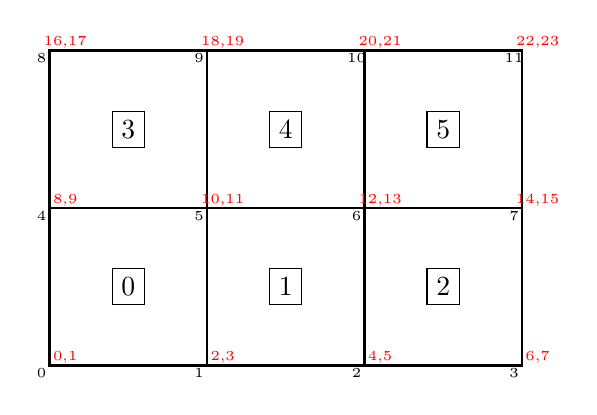
\begin{tikzpicture}
%\draw[step=0.5cm,gray,very thin] (0,0) grid (8,6); %background grid
\draw[thick] (1,1) -- (3,1) -- (3,3) -- (1,3) -- cycle;  
\draw[thick] (3,1) -- (5,1) -- (5,3) -- (3,3) -- cycle; 
\draw[thick] (5,1) -- (7,1) -- (7,3) -- (5,3) -- cycle; 
\draw[thick] (1,3) -- (3,3) -- (3,5) -- (1,5) -- cycle;  
\draw[thick] (3,3) -- (5,3) -- (5,5) -- (3,5) -- cycle; 
\draw[thick] (5,3) -- (7,3) -- (7,5) -- (5,5) -- cycle; 
\node[draw] at (2,2) {0};
\node[draw] at (4,2) {1};
\node[draw] at (6,2) {2};
\node[draw] at (2,4) {3};
\node[draw] at (4,4) {4};
\node[draw] at (6,4) {5};
%pressure dofs
\node at (0.9,0.9) {\tiny 0};
\node at (2.9,0.9) {\tiny 1};
\node at (4.9,0.9) {\tiny 2};
\node at (6.9,0.9) {\tiny 3};
\node at (0.9,2.9) {\tiny 4};
\node at (2.9,2.9) {\tiny 5};
\node at (4.9,2.9) {\tiny 6};
\node at (6.9,2.9) {\tiny 7};
\node at (0.9,4.9) {\tiny 8};
\node at (2.9,4.9) {\tiny 9};
\node at (4.9,4.9) {\tiny 10};
\node at (6.9,4.9) {\tiny 11};
%velocity dofs
\node[red] at (1.2,1.1) {\tiny 0,1};
\node[red] at (3.2,1.1) {\tiny 2,3};
\node[red] at (5.2,1.1) {\tiny 4,5};
\node[red] at (7.2,1.1) {\tiny 6,7};
\node[red] at (1.2,3.1) {\tiny 8,9};
\node[red] at (3.2,3.1) {\tiny 10,11};
\node[red] at (5.2,3.1) {\tiny 12,13};
\node[red] at (7.2,3.1) {\tiny 14,15};
\node[red] at (1.2,5.1) {\tiny 16,17};
\node[red] at (3.2,5.1) {\tiny 18,19};
\node[red] at (5.2,5.1) {\tiny 20,21};
\node[red] at (7.2,5.1) {\tiny 22,23};
\end{tikzpicture}
\end{center}




The $\K$ matrix is of size $NfemV \times NfemV$ with $NfemV=ndofV \times nnp = 2\times 12=24$.
The $\G$ matrix is of size $NfemV \times NfemP$ with $NfemP=ndofP \times nnp = 1\times 12=12$.
The $\C$ matrix is of size $NfemP \times NfemP$. 

A corner pdof sees 4 vdofs, a side pdof sees 12 vdofs and an inside pdof sees 18 vdofs, so that 
the total number of nonzeros in $\G$ can be computed as follows:
\[
NZ_\G = \underbrace{4}_{corners} + 
\underbrace{2(nnx-2)*12}_{2 hor. sides} 
+ 
\underbrace{2(nny-2)*12}_{2 vert. sides} 
+ 
\underbrace{(nnx-2)(nny-2)*18}_{inside nodes}
\]
Concretely, 
\begin{itemize}
\item pdof $\#0$ sees vdofs 0,1,2,3,8,9,10,11
\item pdof $\#1$ sees vdofs 0,1,2,3,4,5,8,9,10,11,12,13
\item pdof $\#5$ sees vdofs 0,1,2,3,4,5,8,9,10,11,12,13,16,17,18,19,20,21
\end{itemize}
so that the $\G^T$ matrix non-zero structure then is as follows:


\begin{center}
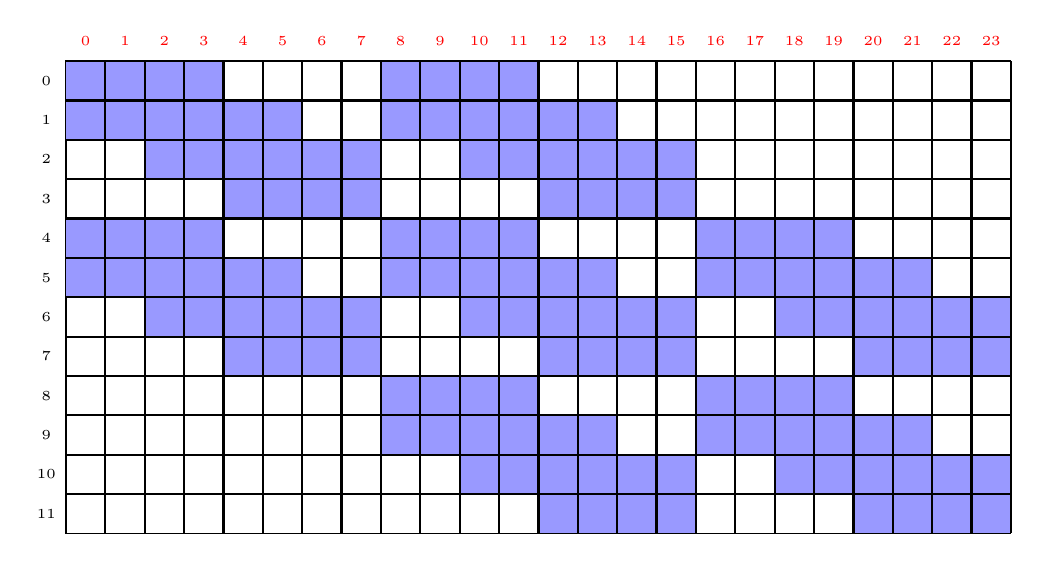
\begin{tikzpicture}
%\draw[step=0.5cm,gray,very thin] (0,0) grid (14,8); %background grid
\draw (1,1) -- (13,1) -- (13,7) -- (1,7) -- cycle;    %matrix
%first top line
\fill[blue!40!white] (1.0,6.5) rectangle (1.5,7);
\fill[blue!40!white] (1.5,6.5) rectangle (2.0,7);
\fill[blue!40!white] (2.0,6.5) rectangle (2.5,7);
\fill[blue!40!white] (2.5,6.5) rectangle (3.0,7);
\fill[blue!40!white] (5.0,6.5) rectangle (5.5,7);
\fill[blue!40!white] (5.5,6.5) rectangle (6.0,7);
\fill[blue!40!white] (6.0,6.5) rectangle (6.5,7);
\fill[blue!40!white] (6.5,6.5) rectangle (7.0,7);
%second line
\fill[blue!40!white] (1.0,6.) rectangle (1.5,6.5);
\fill[blue!40!white] (1.5,6.) rectangle (2.0,6.5);
\fill[blue!40!white] (2.0,6.) rectangle (2.5,6.5);
\fill[blue!40!white] (2.5,6.) rectangle (3.0,6.5);
\fill[blue!40!white] (3.0,6.) rectangle (3.5,6.5);
\fill[blue!40!white] (3.5,6.) rectangle (4.0,6.5);
\fill[blue!40!white] (5.0,6.) rectangle (5.5,6.5);
\fill[blue!40!white] (5.5,6.) rectangle (6.0,6.5);
\fill[blue!40!white] (6.0,6.) rectangle (6.5,6.5);
\fill[blue!40!white] (6.5,6.) rectangle (7.0,6.5);
\fill[blue!40!white] (7.0,6.) rectangle (7.5,6.5);
\fill[blue!40!white] (7.5,6.) rectangle (8.0,6.5);
%third line
\fill[blue!40!white] (2.0,5.5) rectangle (2.5,6.0);
\fill[blue!40!white] (2.5,5.5) rectangle (3.0,6.0);
\fill[blue!40!white] (3.0,5.5) rectangle (3.5,6.0);
\fill[blue!40!white] (3.5,5.5) rectangle (4.0,6.0);
\fill[blue!40!white] (4.0,5.5) rectangle (4.5,6.0);
\fill[blue!40!white] (4.5,5.5) rectangle (5.0,6.0);
\fill[blue!40!white] (6.0,5.5) rectangle (6.5,6.0);
\fill[blue!40!white] (6.5,5.5) rectangle (7.0,6.0);
\fill[blue!40!white] (7.0,5.5) rectangle (7.5,6.0);
\fill[blue!40!white] (7.5,5.5) rectangle (8.0,6.0);
\fill[blue!40!white] (8.0,5.5) rectangle (8.5,6.0);
\fill[blue!40!white] (8.5,5.5) rectangle (9.0,6.0);
%fourth line
\fill[blue!40!white] (3.0,5.) rectangle (3.5,5.5);
\fill[blue!40!white] (3.5,5.) rectangle (4.0,5.5);
\fill[blue!40!white] (4.0,5.) rectangle (4.5,5.5);
\fill[blue!40!white] (4.5,5.) rectangle (5.0,5.5);
\fill[blue!40!white] (7.0,5.) rectangle (7.5,5.5);
\fill[blue!40!white] (7.5,5.) rectangle (8.0,5.5);
\fill[blue!40!white] (8.0,5.) rectangle (8.5,5.5);
\fill[blue!40!white] (8.5,5.) rectangle (9.0,5.5);
%fifth line
\fill[blue!40!white] (1.0,4.5) rectangle (1.5,5);
\fill[blue!40!white] (1.5,4.5) rectangle (2.0,5);
\fill[blue!40!white] (2.0,4.5) rectangle (2.5,5);
\fill[blue!40!white] (2.5,4.5) rectangle (3.0,5);
\fill[blue!40!white] (5.0,4.5) rectangle (5.5,5);
\fill[blue!40!white] (5.5,4.5) rectangle (6.0,5);
\fill[blue!40!white] (6.0,4.5) rectangle (6.5,5);
\fill[blue!40!white] (6.5,4.5) rectangle (7.0,5);
\fill[blue!40!white] (9.0,4.5) rectangle (9.5,5);
\fill[blue!40!white] (9.5,4.5) rectangle (10.0,5);
\fill[blue!40!white] (10.0,4.5) rectangle (10.5,5);
\fill[blue!40!white] (10.5,4.5) rectangle (11.0,5);

%sixth line
\fill[blue!40!white] (1.0,4) rectangle (1.5,4.50);
\fill[blue!40!white] (1.5,4) rectangle (2.0,4.50);
\fill[blue!40!white] (2.0,4) rectangle (2.5,4.50);
\fill[blue!40!white] (2.5,4) rectangle (3.0,4.50);
\fill[blue!40!white] (3.0,4) rectangle (3.5,4.50);
\fill[blue!40!white] (3.5,4) rectangle (4.0,4.50);


\fill[blue!40!white] (5.0,4) rectangle (5.5,4.50);
\fill[blue!40!white] (5.5,4) rectangle (6.0,4.50);
\fill[blue!40!white] (6.0,4) rectangle (6.5,4.50);
\fill[blue!40!white] (6.5,4) rectangle (7.0,4.50);
\fill[blue!40!white] (7.0,4) rectangle (7.5,4.50);
\fill[blue!40!white] (7.5,4) rectangle (8.0,4.50);

\fill[blue!40!white] (9.0,4) rectangle (9.5,4.50);
\fill[blue!40!white] (9.5,4) rectangle (10.0,4.50);
\fill[blue!40!white] (10.0,4) rectangle (10.5,4.50);
\fill[blue!40!white] (10.5,4) rectangle (11.0,4.50);
\fill[blue!40!white] (11.0,4) rectangle (11.5,4.50);
\fill[blue!40!white] (11.5,4) rectangle (12.0,4.50);

%seventh line
\fill[blue!40!white] (2.0,3.5) rectangle (2.5,4.0);
\fill[blue!40!white] (2.5,3.5) rectangle (3.0,4.0);
\fill[blue!40!white] (3.0,3.5) rectangle (3.5,4.0);
\fill[blue!40!white] (3.5,3.5) rectangle (4.0,4.0);
\fill[blue!40!white] (4.0,3.5) rectangle (4.5,4.0);
\fill[blue!40!white] (4.5,3.5) rectangle (5.0,4.0);
\fill[blue!40!white] (6.0,3.5) rectangle (6.5,4.0);
\fill[blue!40!white] (6.5,3.5) rectangle (7.0,4.0);
\fill[blue!40!white] (7.0,3.5) rectangle (7.5,4.0);
\fill[blue!40!white] (7.5,3.5) rectangle (8.0,4.0);
\fill[blue!40!white] (8.0,3.5) rectangle (8.5,4.0);
\fill[blue!40!white] (8.5,3.5) rectangle (9.0,4.0);
\fill[blue!40!white] (10.0,3.5) rectangle (10.5,4.0);
\fill[blue!40!white] (10.5,3.5) rectangle (11.0,4.0);
\fill[blue!40!white] (11.0,3.5) rectangle (11.5,4.0);
\fill[blue!40!white] (11.5,3.5) rectangle (12.0,4.0);
\fill[blue!40!white] (12.0,3.5) rectangle (12.5,4.0);
\fill[blue!40!white] (12.5,3.5) rectangle (13.0,4.0);
%eighth line
\fill[blue!40!white] (3.0,3.) rectangle (3.5,3.5);
\fill[blue!40!white] (3.5,3.) rectangle (4.0,3.5);
\fill[blue!40!white] (4.0,3.) rectangle (4.5,3.5);
\fill[blue!40!white] (4.5,3.) rectangle (5.0,3.5);
\fill[blue!40!white] (7.0,3.) rectangle (7.5,3.5);
\fill[blue!40!white] (7.5,3.) rectangle (8.0,3.5);
\fill[blue!40!white] (8.0,3.) rectangle (8.5,3.5);
\fill[blue!40!white] (8.5,3.) rectangle (9.0,3.5);
\fill[blue!40!white] (11.0,3.) rectangle (11.5,3.5);
\fill[blue!40!white] (11.5,3.) rectangle (12.0,3.5);
\fill[blue!40!white] (12.0,3.) rectangle (12.5,3.5);
\fill[blue!40!white] (12.5,3.) rectangle (13.0,3.5);
%9th line
\fill[blue!40!white] (5.0,2.5) rectangle (5.5,3);
\fill[blue!40!white] (5.5,2.5) rectangle (6.0,3);
\fill[blue!40!white] (6.0,2.5) rectangle (6.5,3);
\fill[blue!40!white] (6.5,2.5) rectangle (7.0,3);
\fill[blue!40!white] (9.0,2.5) rectangle (9.5,3);
\fill[blue!40!white] (9.5,2.5) rectangle (10.0,3);
\fill[blue!40!white] (10.0,2.5) rectangle (10.5,3);
\fill[blue!40!white] (10.5,2.5) rectangle (11.0,3);
%10th line
\fill[blue!40!white] (5.0,2) rectangle (5.5,2.5);
\fill[blue!40!white] (5.5,2) rectangle (6.0,2.5);
\fill[blue!40!white] (6.0,2) rectangle (6.5,2.5);
\fill[blue!40!white] (6.5,2) rectangle (7.0,2.5);
\fill[blue!40!white] (7.0,2) rectangle (7.5,2.5);
\fill[blue!40!white] (7.5,2) rectangle (8.0,2.5);
\fill[blue!40!white] (9.0,2) rectangle (9.5,2.5);
\fill[blue!40!white] (9.5,2) rectangle (10.0,2.5);
\fill[blue!40!white] (10.0,2) rectangle (10.5,2.5);
\fill[blue!40!white] (10.5,2) rectangle (11.0,2.5);
\fill[blue!40!white] (11.0,2) rectangle (11.5,2.5);
\fill[blue!40!white] (11.5,2) rectangle (12.0,2.5);
%11th line
\fill[blue!40!white] (6.0,1.5) rectangle (6.5,2);
\fill[blue!40!white] (6.5,1.5) rectangle (8,2);
\fill[blue!40!white] (7.0,1.5) rectangle (7.5,2);
\fill[blue!40!white] (7.5,1.5) rectangle (8.0,2);
\fill[blue!40!white] (8.0,1.5) rectangle (8.5,2);
\fill[blue!40!white] (8.5,1.5) rectangle (9.0,2);
\fill[blue!40!white] (10.0,1.5) rectangle (10.5,2);
\fill[blue!40!white] (10.5,1.5) rectangle (11.0,2);
\fill[blue!40!white] (11.0,1.5) rectangle (11.5,2);
\fill[blue!40!white] (11.5,1.5) rectangle (12.0,2);
\fill[blue!40!white] (12.0,1.5) rectangle (12.5,2);
\fill[blue!40!white] (12.5,1.5) rectangle (13.0,2);
%12th line
\fill[blue!40!white] (7.0,1.0) rectangle (7.5,1.5);
\fill[blue!40!white] (7.5,1.0) rectangle (8.0,1.5);
\fill[blue!40!white] (8.0,1.0) rectangle (8.5,1.5);
\fill[blue!40!white] (8.5,1.0) rectangle (9.0,1.5);
\fill[blue!40!white] (11.0,1.0) rectangle (11.5,1.5);
\fill[blue!40!white] (11.5,1.0) rectangle (12.0,1.5);
\fill[blue!40!white] (12.0,1.0) rectangle (12.5,1.5);
\fill[blue!40!white] (12.5,1.0) rectangle (13.0,1.5);
%vertical
\node at (0.75,6.75) {\tiny 0};
\node at (0.75,6.25) {\tiny 1};
\node at (0.75,5.75) {\tiny 2};
\node at (0.75,5.25) {\tiny 3};
\node at (0.75,4.75) {\tiny 4};
\node at (0.75,4.25) {\tiny 5};
\node at (0.75,3.75) {\tiny 6};
\node at (0.75,3.25) {\tiny 7};
\node at (0.75,2.75) {\tiny 8};
\node at (0.75,2.25) {\tiny 9};
\node at (0.75,1.75) {\tiny 10};
\node at (0.75,1.25) {\tiny 11};
%horizontal
\node[red] at (1.25,7.25) {\tiny 0};
\node[red] at (1.75,7.25) {\tiny 1};
\node[red] at (2.25,7.25) {\tiny 2};
\node[red] at (2.75,7.25) {\tiny 3};
\node[red] at (3.25,7.25) {\tiny 4};
\node[red] at (3.75,7.25) {\tiny 5};
\node[red] at (4.25,7.25) {\tiny 6};
\node[red] at (4.75,7.25) {\tiny 7};
\node[red] at (5.25,7.25) {\tiny 8};
\node[red] at (5.75,7.25) {\tiny 9};
\node[red] at (6.25,7.25) {\tiny 10};
\node[red] at (6.75,7.25) {\tiny 11};
\node[red] at (7.25,7.25) {\tiny 12};
\node[red] at (7.75,7.25) {\tiny 13};
\node[red] at (8.25,7.25) {\tiny 14};
\node[red] at (8.75,7.25) {\tiny 15};
\node[red] at (9.25,7.25) {\tiny 16};
\node[red] at (9.75,7.25) {\tiny 17};
\node[red] at (10.25,7.25) {\tiny 18};
\node[red] at (10.75,7.25) {\tiny 19};
\node[red] at (11.25,7.25) {\tiny 20};
\node[red] at (11.75,7.25) {\tiny 21};
\node[red] at (12.25,7.25) {\tiny 22};
\node[red] at (12.75,7.25) {\tiny 23};
\draw[step=0.5cm,black,thick] (1,1) grid (13,7); %background grid
\end{tikzpicture}
\end{center}










%-------------------------------------------------------------
\subsection*{Non-zero pattern of the $\C$ matrix}

Concretely, 
\begin{itemize}
\item pdof $\#0$ sees vdofs 0,1,4,5
\item pdof $\#1$ sees vdofs 0,1,2,4,5,6
\item pdof $\#5$ sees vdofs 0,1,2,4,5,6,8,9,10
\end{itemize}
so that the $\C$ matrix non-zero structure is as follows:


\begin{center}
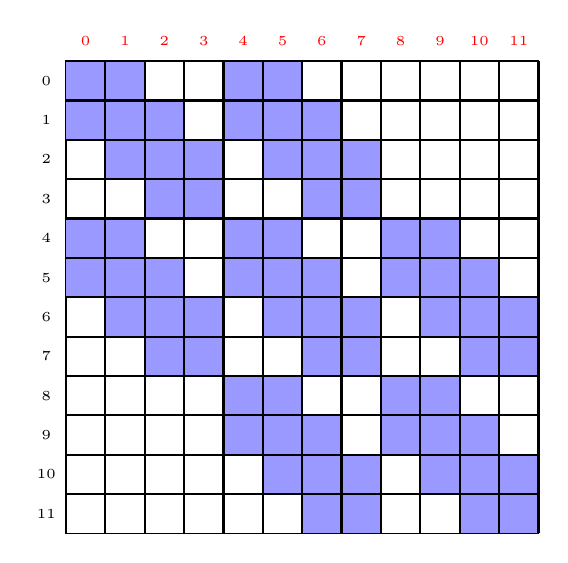
\begin{tikzpicture}
%\draw[step=0.5cm,gray,very thin] (0,0) grid (9,9); %background grid
\draw (1,1) -- (7,1) -- (7,7) -- (1,7) -- cycle;    %matrix

%vertical
\node at (0.75,6.75) {\tiny 0};
\node at (0.75,6.25) {\tiny 1};
\node at (0.75,5.75) {\tiny 2};
\node at (0.75,5.25) {\tiny 3};
\node at (0.75,4.75) {\tiny 4};
\node at (0.75,4.25) {\tiny 5};
\node at (0.75,3.75) {\tiny 6};
\node at (0.75,3.25) {\tiny 7};
\node at (0.75,2.75) {\tiny 8};
\node at (0.75,2.25) {\tiny 9};
\node at (0.75,1.75) {\tiny 10};
\node at (0.75,1.25) {\tiny 11};

%horizontal
\node[red] at (1.25,7.25) {\tiny 0};
\node[red] at (1.75,7.25) {\tiny 1};
\node[red] at (2.25,7.25) {\tiny 2};
\node[red] at (2.75,7.25) {\tiny 3};
\node[red] at (3.25,7.25) {\tiny 4};
\node[red] at (3.75,7.25) {\tiny 5};
\node[red] at (4.25,7.25) {\tiny 6};
\node[red] at (4.75,7.25) {\tiny 7};
\node[red] at (5.25,7.25) {\tiny 8};
\node[red] at (5.75,7.25) {\tiny 9};
\node[red] at (6.25,7.25) {\tiny 10};
\node[red] at (6.75,7.25) {\tiny 11};

%first top line
\fill[blue!40!white] (1.0,6.5) rectangle (1.5,7);
\fill[blue!40!white] (1.5,6.5) rectangle (2.0,7);
\fill[blue!40!white] (3.0,6.5) rectangle (3.5,7);
\fill[blue!40!white] (3.5,6.5) rectangle (4.0,7);
%second line
\fill[blue!40!white] (1.0,6.) rectangle (1.5,6.5);
\fill[blue!40!white] (1.5,6.) rectangle (2.0,6.5);
\fill[blue!40!white] (2.0,6.) rectangle (2.5,6.5);
\fill[blue!40!white] (3.0,6.) rectangle (3.5,6.5);
\fill[blue!40!white] (3.5,6.) rectangle (4.0,6.5);
\fill[blue!40!white] (4.0,6.) rectangle (4.5,6.5);
%third line
\fill[blue!40!white] (1.5,5.5) rectangle (2.0,6.);
\fill[blue!40!white] (2.0,5.5) rectangle (2.5,6.);
\fill[blue!40!white] (2.5,5.5) rectangle (3.0,6.);
\fill[blue!40!white] (3.5,5.5) rectangle (4.0,6.);
\fill[blue!40!white] (4.0,5.5) rectangle (4.5,6.);
\fill[blue!40!white] (4.5,5.5) rectangle (5.0,6.);
%fourth line
\fill[blue!40!white] (2.0,5.) rectangle (2.5,5.5);
\fill[blue!40!white] (2.5,5.) rectangle (3.0,5.5);
\fill[blue!40!white] (4.0,5.) rectangle (4.5,5.5);
\fill[blue!40!white] (4.5,5.) rectangle (5.0,5.5);
%fifth line
\fill[blue!40!white] (1.0,4.5) rectangle (1.5,5.);
\fill[blue!40!white] (1.5,4.5) rectangle (2.0,5.);
\fill[blue!40!white] (3.0,4.5) rectangle (3.5,5.);
\fill[blue!40!white] (3.5,4.5) rectangle (4.0,5.);
\fill[blue!40!white] (5.0,4.5) rectangle (5.5,5.);
\fill[blue!40!white] (5.5,4.5) rectangle (6.0,5.);
%sixth line
\fill[blue!40!white] (1.0,4.) rectangle (1.5,4.5);
\fill[blue!40!white] (1.5,4.) rectangle (2.0,4.5);
\fill[blue!40!white] (2.0,4.) rectangle (2.5,4.5);
\fill[blue!40!white] (3.0,4.) rectangle (3.5,4.5);
\fill[blue!40!white] (3.5,4.) rectangle (4.0,4.5);
\fill[blue!40!white] (4.0,4.) rectangle (4.5,4.5);
\fill[blue!40!white] (5.0,4.) rectangle (5.5,4.5);
\fill[blue!40!white] (5.5,4.) rectangle (6.0,4.5);
\fill[blue!40!white] (6.0,4.) rectangle (6.5,4.5);
%seventh line
\fill[blue!40!white] (1.5,3.5) rectangle (2.0,4.);
\fill[blue!40!white] (2.0,3.5) rectangle (2.5,4.);
\fill[blue!40!white] (2.5,3.5) rectangle (3.0,4.);
\fill[blue!40!white] (3.5,3.5) rectangle (4.0,4.);
\fill[blue!40!white] (4.0,3.5) rectangle (4.5,4.);
\fill[blue!40!white] (4.5,3.5) rectangle (5.0,4.);
\fill[blue!40!white] (5.5,3.5) rectangle (6.0,4.);
\fill[blue!40!white] (6.0,3.5) rectangle (6.5,4.);
\fill[blue!40!white] (6.5,3.5) rectangle (7.0,4.);
%eighth line
\fill[blue!40!white] (2.0,3.) rectangle (2.5,3.5);
\fill[blue!40!white] (2.5,3.) rectangle (3.0,3.5);
\fill[blue!40!white] (4.0,3.) rectangle (4.5,3.5);
\fill[blue!40!white] (4.5,3.) rectangle (5.0,3.5);
\fill[blue!40!white] (6.0,3.) rectangle (6.5,3.5);
\fill[blue!40!white] (6.5,3.) rectangle (7.0,3.5);
%ninth line
\fill[blue!40!white] (3.0,2.5) rectangle (3.5,3.);
\fill[blue!40!white] (3.5,2.5) rectangle (4.0,3.);
\fill[blue!40!white] (5.0,2.5) rectangle (5.5,3.);
\fill[blue!40!white] (5.5,2.5) rectangle (6.0,3.);
%tenth line
\fill[blue!40!white] (3.0,2.) rectangle (3.5,2.5);
\fill[blue!40!white] (3.5,2.) rectangle (4.0,2.5);
\fill[blue!40!white] (4.0,2.) rectangle (4.5,2.5);
\fill[blue!40!white] (5.0,2.) rectangle (5.5,2.5);
\fill[blue!40!white] (5.5,2.) rectangle (6.0,2.5);
\fill[blue!40!white] (6.0,2.) rectangle (6.5,2.5);
%eleventh line
\fill[blue!40!white] (3.5,1.5) rectangle (4.0,2.);
\fill[blue!40!white] (4.0,1.5) rectangle (4.5,2.);
\fill[blue!40!white] (4.5,1.5) rectangle (5.0,2.);
\fill[blue!40!white] (5.5,1.5) rectangle (6.0,2.);
\fill[blue!40!white] (6.0,1.5) rectangle (6.5,2.);
\fill[blue!40!white] (6.5,1.5) rectangle (7.0,2.);
%twelfth line
\fill[blue!40!white] (4.0,1.) rectangle (4.5,1.5);
\fill[blue!40!white] (4.5,1.) rectangle (5.0,1.5);
\fill[blue!40!white] (6.0,1.) rectangle (6.5,1.5);
\fill[blue!40!white] (6.5,1.) rectangle (7.0,1.5);


\draw[step=0.5cm,black,thick] (1,1) grid (7,7); %background grid





\end{tikzpicture}
\end{center}





%-------------------------------------------------------------
\subsection*{Constraining the pressure field to zero average}

We impose $\int p dV=0$ which means that the following constraint is added 
to the Stokes matrix:
\[
\left(
\begin{array}{ccc}
\K & \G & 0\\ 
\G^T & \C & \LLL \\
0 & \LLL^T & 0 
\end{array}
\right)
\cdot
\left(
\begin{array}{c}
{\cal V} \\ {\cal P} \\ \lambda
\end{array}
\right)
=
\left(
\begin{array}{c}
 f \\ h \\ 0
\end{array}
\right)
\]




%---------------------------------------------------
\subsection*{The Donea \& Huerta benchmark (case 1)}

As in \cite{dohu03} we solve the benchmark problem presented in section \ref{mms1}.

\begin{center}
\includegraphics[width=10cm]{python_codes/fieldstone_22/results/case1/errors.pdf}
\end{center}

%------------------------------------------------------
\subsection*{The Dohrmann \& Bochev benchmark (case 2)} 

As in \cite{dobo04} we solve the benchmark problem presented in section \ref{mms2}.

\begin{center}
\includegraphics[width=10cm]{python_codes/fieldstone_22/results/case2/errors.pdf}
\end{center}

\todo[inline]{compare my rates with original paper!}

%\includegraphics[width=5cm]{python_codes/fieldstone_22/results/uth}
%\includegraphics[width=5cm]{python_codes/fieldstone_22/results/vth}
%\includegraphics[width=5cm]{python_codes/fieldstone_22/results/pth}

%--------------------------------------------------
\subsection*{The sinking block experiment (case 3)} 

The setup is described in \cite{thba20}. 
It consists of a two-dimensional $512\times 512$km domain filled with a fluid (the "mantle") 
of density $\rho_1=3200$kg/m$^3$ and viscosity $\eta_1$. A square block of 
size $128\times 128$km is placed in the domain and is centered at location 
($x_c,y_c$)=(256km,384km) so as to insure that its sides align with cell boundaries at 
all resolutions. It is filled with a fluid of density $\rho_2=\rho_1+\delta \rho$ 
and viscosity $\eta_2$. The gravity vector points downwards with $|\vec{g}|=10$m/s$^2$. 
Boundary conditions are free slip on all sides. Only one time step is carried out and 
we measure the velocity $|v_z|$ in the middle of the block. 

\begin{center}
\includegraphics[width=13cm]{python_codes/fieldstone_22/results/case3/blocks}
\end{center}

\begin{center}
\includegraphics[width=5cm]{python_codes/fieldstone_22/results/case3/fallingblock_sub1.pdf}
\includegraphics[width=5cm]{python_codes/fieldstone_22/results/case3/fallingblock_sub2.pdf}
\includegraphics[width=5cm]{python_codes/fieldstone_22/results/case3/fallingblock_sub3.pdf}\\
{\captionfont From left to right: subcase=1,2,3.}
\end{center}

\begin{center}
\includegraphics[width=12cm]{python_codes/fieldstone_22/results/case3/u123}
\includegraphics[width=12cm]{python_codes/fieldstone_22/results/case3/v123}\\
{\captionfont From left to right: subcase=1,2,3. 
Resolution 96x96, $\delta \rho=32$, $\eta_2=10^{23}$}
\end{center}





%-----------------------------------------
\subsection*{SolCx (case 4)} 

This benchmark is described in Section~\ref{mms:solcx}.

\begin{center}
\includegraphics[width=10cm]{python_codes/fieldstone_22/results/case4/errors.pdf}\\
{\captionfont Resolutions 8x8 to 96x96. Even resolutions converge ${\cal O}(h^2)$ 
for velocity while \\ even resolutions converge ${\cal O}(h^1)$. In both cases the \\
pressure converges ${\cal O}(h^{1/2})$.}
\end{center}


%-----------------------------------------
\subsection*{SolVi (case 5)} 

This benchmark is described in Section~\ref{mms:solvi}.

\begin{center}
\includegraphics[width=10cm]{python_codes/fieldstone_22/results/case5/errors.pdf}\\
{\captionfont Resolutions 8x8 to 96x96.} 
\end{center}

\begin{center}
\includegraphics[width=7cm]{python_codes/fieldstone_22/results/case5/veldiag}
\includegraphics[width=7cm]{python_codes/fieldstone_22/results/case5/pressbottom}\\
{\captionfont Velocity and pressure on the diagonal $y=x$, at resolution 96x96.} 
\end{center}

\begin{center}
\includegraphics[width=5cm]{python_codes/fieldstone_22/results/case5/vel}
\includegraphics[width=5cm]{python_codes/fieldstone_22/results/case5/vel2}
\includegraphics[width=5cm]{python_codes/fieldstone_22/results/case5/p}\\
\end{center}





\newpage %%%%%%%%%%%%%%%%%%%%%%%%%%%%%%%%%%%%%%%%%%%%%%%%%%%%%%%%%%%%%%%%%%%%%%%%%%%%%%%%
\section*{
Stone 23: compressible flow (1) - analytical benchmark 
\label{f23}}
\addcontentsline{toc}{section}{\protect\numberline{} 
Stone 23: compressible flow (1) - analytical benchmark 
}

\index{stones}{$Q_1 \times P_0$ element}
\index{stones}{Mixed Formulation}
\index{stones}{Analytical Solution}
\index{stones}{Pressure Smoothing} 

\begin{mdframed}[backgroundcolor=red!5]
This work is part of the MSc thesis of T. Weir (2018).
\end{mdframed}
\index{contributors}{T. Weir}

We first start with an isothermal Stokes flow, so that we disregard the heat transport equation and 
the equations we wish to solve are simply:

\begin{align}
  \label{eq:stokes-1}
  -\nabla \cdot \left[2\eta \left(\dot\varepsilon(\bm v)
                                  - \frac{1}{3}(\nabla \cdot \bm v)\mathbf 1\right)
                \right] + \nabla p &=
  \rho \bm g
  &
  & \textrm{in $\Omega$},
  \\
  \label{eq:stokes-2}
  \nabla \cdot (\rho \bm v) &= 0
  &
  & \textrm{in $\Omega$}
\end{align}
The second equation can be rewritten 
$\nabla \cdot (\rho {\bm v}) =  \rho \nabla \cdot {\bm v} + {\bm v} \cdot {\bm \nabla}\rho=0$
or, 
\[
\nabla \cdot {\bm v} + \frac{1}{\rho} {\bm v} \cdot {\bm \nabla}\rho=0
\]
Note that this presupposes that the density is not zero anywhere in the domain.

We use a mixed formulation and therefore  
keep both velocity and pressure as unknowns. We end up having to solve 
the following system:
\[
\left(
\begin{array}{cc}
\K & \G \\ \G^T+\Z & 0 
\end{array}
\right)
\cdot
\left(
\begin{array}{c}
{\cal V} \\ {\cal P}
\end{array}
\right)
=
\left(
\begin{array}{c}
 f \\ h
\end{array}
\right)
\quad\quad
{\rm or,}
\quad\quad
\A \cdot X = rhs
\]
Where $\K$ is the stiffness matrix, $\G$ is the discrete gradient operator, 
$\G^T$ is the discrete divergence operator, ${\cal V}$ the velocity vector, 
${\cal P}$ the pressure vector.
Note that the term $\Z{\cal V}$ derives from term ${\bm v} \cdot {\bm \nabla} \rho$ in the continuity equation. 

Each block $\K$, $\G$ , $\Z$ and vectors $f$ and $h$ are built separately 
in the code and assembled into 
the matrix $\A$ and vector $rhs$ afterwards. $\A$ and $rhs$ are then passed to the solver. 
We will see later that there are alternatives to solve this approach which do not require to 
build the full Stokes matrix $\A$. 

{\sl Remark}: the term $\Z {\cal V}$ is often put in the rhs (i.e. added to $h$) so that 
the matrix $\A$ retains the same structure as in the incompressible case. This is indeed 
how it is implemented in ASPECT. This however requires more work since the rhs depends 
on the solution and some form of iterations is needed. 

In the case of a compressible flow the strain rate tensor and the deviatoric strain rate tensor are no more equal (since ${\bm \nabla}\cdot{\bm v} \neq 0$).
The deviatoric strainrate tensor is given by\footnote{See the ASPECT manual for a justification of the 3 value in the denominator in 2D and 3D.} 
\[
\dot{\bm \epsilon}^d({\bm v})=
\dot{\bm \epsilon}({\bm v})-\frac{1}{3} Tr(\dot{\bm \epsilon}) {\bm 1}
=\dot{\bm \epsilon}({\bm v})-\frac{1}{3} ({\bm \nabla}\cdot{\bm v}) {\bm 1}
\]
In that case:
\begin{eqnarray}
\dot{\epsilon}_{xx}^d 
&=& \frac{\partial u}{\partial x}
-\frac{1}{3} \left( \frac{\partial u}{\partial x} + \frac{\partial v}{\partial y} \right) 
= \frac{2}{3}\frac{\partial u}{\partial x}
-\frac{1}{3} \frac{\partial v}{\partial y}
%=
%\frac{2}{3} \sum_{i=1}^4 \frac{\partial N_i}{\partial x}\;  u_i 
%-\frac{1}{3} \sum_{i=1}^4 \frac{\partial N_i}{\partial y}\;  v_i 
\\
\dot{\epsilon}_{yy}^d 
&=& \frac{\partial v}{\partial y}
-\frac{1}{3} \left( \frac{\partial u}{\partial x} + \frac{\partial v}{\partial y} \right) 
=-\frac{1}{3} \frac{\partial u}{\partial x} 
+ \frac{2}{3} \frac{\partial v}{\partial y} 
%=-\frac{1}{3}  \sum_{i=1}^4 \frac{\partial N_i}{\partial x}\;  u_i
%+ \frac{2}{3} \sum_{i=1}^4 \frac{\partial N_i}{\partial y}\;  v_i
\\
2\dot{\epsilon}_{xy}^d 
&=& 
\frac{\partial u}{\partial y} 
+\frac{\partial v}{\partial x} 
%= \sum_{i=1}^4 \frac{\partial N_i}{\partial y}\;  u_i
%+ \sum_{i=1}^4 \frac{\partial N_i}{\partial x}\;  v_i
\end{eqnarray}
and then 
\[
\dot{\bm \epsilon}^d({\bm v})
=
\left(
\begin{array}{cc}
\frac{2}{3} \frac{\partial u}{\partial x} -\frac{1}{3} \frac{\partial v}{\partial y} &
\frac{1}{2}\frac{\partial u}{\partial y} + \frac{1}{2}\frac{\partial v}{\partial x}  \\ \\
\frac{1}{2}\frac{\partial u}{\partial y} + \frac{1}{2}\frac{\partial v}{\partial x}  &
-\frac{1}{3} \frac{\partial u}{\partial x} +\frac{2}{3} \frac{\partial v}{\partial y} 
\end{array}
\right)
\]

From $\vec{\tau} = 2\eta \vec{\epsilon}^d$ we arrive at:
\[
\left(
\begin{array}{c}
\tau_{xx}\\
\tau_{yy}\\
\tau_{xy}\\
\end{array}
\right)
=
2\eta
\left(
\begin{array}{c}
\dot{\epsilon}_{xx}^d \\
\dot{\epsilon}_{yy}^d \\
\dot{\epsilon}_{xy}^d 
\end{array}
\right)
=2 \eta
\left(
\begin{array}{ccc}
2/3 & -1/3& 0 \\
-1/3 & 2/3 & 0 \\
0 & 0 & 1/2 \\
\end{array}
\right)
\cdot 
\left(
\begin{array}{c}
\frac{\partial u}{\partial x} \\ 
\frac{\partial v}{\partial y} \\ 
\frac{\partial u}{\partial y}\! +\! \frac{\partial v}{\partial x} \\
\end{array}
\right)
=
\eta
\left(
\begin{array}{ccc}
4/3 & -2/3& 0 \\
-2/3 & 4/3 & 0 \\
0 & 0 & 1 \\
\end{array}
\right)
\cdot 
\left(
\begin{array}{c}
\frac{\partial u}{\partial x} \\ 
\frac{\partial v}{\partial y} \\ 
\frac{\partial u}{\partial y}\! +\! \frac{\partial v}{\partial x} \\
\end{array}
\right)
\]
or, 
\[
\vec{\tau} = {\bm C}_\eta {\bm B} V
\]


















\newpage
In order to test our implementation we have created a few manufactured solutions:
\begin{itemize}
\item \underline{benchmark \#1} ({\tt ibench=1})): Starting from a density profile of:
\begin{equation}
    \rho(x,y) = xy
\end{equation}
We derive a velocity given by:
\begin{equation}
    v_x(x,y) = \frac{C_x}{x} , v_y(x,y) = \frac{C_y}{y}
\end{equation}

With $g_x(x,y) = \frac{1}{x}$ and $g_y(x,y) = \frac{1}{y}$, this leads us to a pressure profile:
\begin{equation}
    p = - \eta \left( \frac{4C_x}{3x^2} + \frac{4C_y}{3y^2} \right)  + xy + C_0
\end{equation}
This gives us a strain rate:
\[
\dot{\epsilon}_{xx} =  \frac{-C_x}{x^2}
\quad
\quad
\quad
\dot{\epsilon}_{yy} =  \frac{-C_y}{y^2}
\quad
\quad
\quad
\dot{\epsilon}_{xy} = 0 
\]
In what follows, we choose $\eta=1$ and $C_x=C_y=1$ and for a unit square domain $
[1:2]\times[1:2]$ we compute $C_0$
so that the pressure is normalised to zero over the whole domain and obtain $C_0=-1$. 
 
\item \underline{benchmark \#2} ({\tt ibench=2}): Starting from a density profile of:
\begin{equation}
    \rho = \cos(x)\cos(y)
\end{equation}
We derive a velocity given by:
\begin{equation}
    v_x = \frac{C_x}{\cos(x)} , v_y = \frac{C_y}{\cos(y)}
\end{equation}
With $g_x = \frac{1}{\cos(y)}$ and $g_y = \frac{1}{\cos(x)}$, this leads us to a pressure profile:
\begin{equation}
    p =  \eta \Bigg(\frac{4C_x \sin(x)}{3\cos^2(x)} + \frac{4C_y \sin(y)}{3\cos^2(y)}\Bigg) 
    +( \sin(x) + \sin(y) ) + C_0
\end{equation}
\[
\dot{\epsilon}_{xx} = C_x \frac{\sin(x)}{\cos^2(x)}
\quad
\quad
\quad
\dot{\epsilon}_{yy} = C_y \frac{\sin(y)}{\cos^2(y)}
\quad
\quad
\quad
\dot{\epsilon}_{xy} = 0 
\]
We choose $\eta=1$ and $C_x=C_y=1$. The domain is the unit square $[0:1]\times[0:1]$ and we obtain 
$C_0$ as before and obtain 
\[
C_0 = 2 - 2 \cos(1) + 8/3 (\frac{1}{\cos (1)} - 1)
\simeq 3.18823730
\]
(thank you WolframAlpha)


\item \underline{benchmark \#3} ({\tt ibench=3}) 
\item \underline{benchmark \#4} ({\tt ibench=4}) 
\item \underline{benchmark \#5} ({\tt ibench=5}) 
\end{itemize}





%\includegraphics[width=16cm]{python_codes/fieldstone_saddlepoint/solution.pdf}

ToDo:
\begin{itemize}
\item pbs with odd vs even number of elements 
\item q is 'fine' everywhere except in the corners - revisit pressure smoothing paper?
\item redo A v d Berg benchmark (see Tom Weir thesis)
\end{itemize}




\newpage %%%%%%%%%%%%%%%%%%%%%%%%%%%%%%%%%%%%%%%%%%%%%%%%%%%%%%%%%%%%%%%%%%%%%%%%%%%%%%%%
\section*{
Stone 24: compressible flow (2) - convection box 
\label{f24}}
\addcontentsline{toc}{section}{\protect\numberline{} 
Stone 24: compressible flow (2) - convection box 
}
\begin{mdframed}[backgroundcolor=red!5]
This work is part of the MSc thesis of T. Weir (2018).
\end{mdframed}


\subsection*{The physics}

Let us start with some thermodynamics. Every material has an equation of state.
The equilibrium thermodynamic state of any material can
be constrained if any two state variables are specified.
Examples of state variables include
the pressure $p$ and specific volume $\nu = 1/\rho$, as well as the temperature $T$.

After linearisation, the density depends on temperature and pressure as follows:
\[
\rho(T,p) = \rho_0 \left((1 - \alpha(T-T_0) + \beta_T p \right)
\]
where $\alpha$ is the coefficient of thermal expansion, also called 
thermal expansivity: \index{thermal expansion}
\[
\alpha=-\frac{1}{\rho}\left( \frac{\partial \rho}{\partial T} \right)_p
\]
$\alpha$ is the percentage increase in volume of a material per degree of temperature increase; the
subscript $p$ means that the pressure is held fixed.

$\beta_T$ is the isothermal compressibility of the fluid, which is given by \index{compressibility}
\[
\beta_T = \frac{1}{K} = \frac{1}{\rho}\left( \frac{\partial \rho}{\partial P} \right)_T
\]
with $K$ the bulk modulus. \index{bulk modulus}
%aspect manual
Values of $\beta_T=10^{-12}-10^{-11}$ Pa$^{-1}$ are reasonable for Earth's mantle, with values decreasing by about a
factor of 5 between the shallow lithosphere and core-mantle boundary.
This is the percentage increase in density per unit change in pressure at constant temperature.
Both the coefficient of thermal expansion and the isothermal compressibility can be obtained
from the equation of state.

The full set of equations we wish to solve is given by

\begin{eqnarray}
-\nabla \cdot \left[2\eta \dot{\bm \epsilon}^d({\bm v}) \right] + \nabla p &=& \rho_0 \left((1 - \alpha(T-T_0) + \beta_T p \right) {\bm g} \quad\quad \textrm{in $\Omega$}  \label{eq:stokes-1} \\
\nabla \cdot {\bm v} + \frac{1}{\rho} {\bm v} \cdot {\bm \nabla}\rho&=&0 \quad\quad  \textrm{in $\Omega$}   \label{eq:stokes-2} \\
\rho C_p \left(\frac{\partial T}{\partial t} + \bm v\cdot\nabla T\right) - \nabla\cdot k\nabla T   &=& 
  \rho H  +  2\eta \dot{\bm \epsilon}^d : \dot{\bm \epsilon}^d    +\alpha T \left( \frac{\partial p}{\partial t}+  \bm v \cdot \nabla p \right) 
\quad\quad   \textrm{in $\Omega$},
  \label{eq:temperature}
\end{eqnarray}

Note that this presupposes that the density is not zero anywhere in the domain.


\subsection*{The numerics}

We use a mixed formulation and therefore  
keep both velocity and pressure as unknowns. We end up having to solve 
the following system:
\[
\left(
\begin{array}{cc}
\K & \G+\W \\ \G^T+\Z & 0 
\end{array}
\right)
\cdot
\left(
\begin{array}{c}
{\cal V} \\ {\cal P}
\end{array}
\right)
=
\left(
\begin{array}{c}
 f \\ h
\end{array}
\right)
\quad\quad
{\rm or,}
\quad\quad
\A \cdot X = rhs
\]
Where $\K$ is the stiffness matrix, $\G$ is the discrete gradient operator, 
$\G^T$ is the discrete divergence operator, ${\cal V}$ the velocity vector, 
${\cal P}$ the pressure vector.
Note that the term $\Z{\cal V}$ derives from term ${\bm v} \cdot {\bm \nabla} \rho$ in the continuity equation. 

As perfectly explained in the step 32 of deal.ii\footnote{https://www.dealii.org/9.0.0/doxygen/deal.II/step\_32.html},
we need to scale the $\G$ term since it is many orders of magnitude smaller than $\K$, which introduces large inaccuracies in the solving process to the point that the solution is nonsensical. This scaling coefficient is $\eta/L$. After building the $\G$ block, it is then scaled as follows: $\G'=\frac{\eta}{L}\G$ so that we now solve 

\[
\left(
\begin{array}{cc}
\K & \G'+\W \\ \G'^T+\Z & 0 
\end{array}
\right)
\cdot
\left(
\begin{array}{c}
{\cal V} \\ {\cal P}'
\end{array}
\right)
=
\left(
\begin{array}{c}
 f \\ h
\end{array}
\right)
\]
After the solve phase, we recover the real pressure with ${\cal P}=\frac{\eta}{L}{\cal P}'$.

{\color{red} adapt notes since I should scale $\W$ and $\Z$ too}.
{\color{red} $h$ should be caled too !!!!!!!!!!!!!!!} 

Each block $\K$, $\G$ , $\Z$ and vectors $f$ and $h$ are built separately 
in the code and assembled into 
the matrix $\A$ and vector $rhs$ afterwards. $\A$ and $rhs$ are then passed to the solver. 
We will see later that there are alternatives to solve this approach which do not require to 
build the full Stokes matrix $\A$. 

{\bf Remark 1}: the terms $\Z {\cal V}$ and $\W {\cal P}$ are 
often put in the rhs (i.e. added to $h$) so that 
the matrix $\A$ retains the same structure as in the incompressible case. This is indeed 
how it is implemented in ASPECT, see also appendix A of \cite{lezh08}. This however requires more work since the rhs depends 
on the solution and some form of iterations is needed. 

{\bf Remark 2}: Very often the adiabatic heating term  
$\alpha T \left( \bm v \cdot \nabla p \right)$ is simplified as follows:
%aspect manual
If you assume the vertical component of the gradient of the dynamic pressure to be small compared to the
gradient of the total pressure (in other words, the gradient is dominated by the gradient of the hydrostatic
pressure), then $-\rho {\bm g} \simeq {\bm \nabla}p$ and then 
$\alpha T \left( \bm v \cdot \nabla p \right) \simeq  -\alpha\rho T {\bm v}\cdot{\bm g}$. We will however 
not be using this approximation in what follows.



We have already established that
\[
\vec{\tau} = {\bm C}_\eta {\bm B} V
\]


The following measurements are carried out:
\begin{itemize}
\item The root mean square velocity ({\tt vrms}):
\[
v_{rms} = \sqrt{\frac{1}{V}\int_V v^2 dV   }
\]
\item The average temperature ({\tt Tavrg}):
\[
<T>=\frac{1}{V}\int_V T dV
\]
\item The total mass ({\tt mass}):
\[
M=\int_V \rho dV 
\]
\item The Nusselt number ({\tt Nu}):
\[
Nu=-\frac{1}{Lx}\frac{1}{\Delta T} \int_0^{L_x} \frac{\partial T(x,y=L_y)}{\partial y} dx
\]
\item The kinetic energy ({\tt EK}):
\[
E_K=\int_V \frac{1}{2}\rho v^2 dV
\]
\item The work done against gravity 
\[
<W>=-\int_V \rho g_y v_y dV
\]
\item The total viscous dissipation ({\tt visc\_diss})
\[
<\Phi>=\int \Phi dV =\frac{1}{V}\int 2 \eta \dot{\bm \varepsilon}:\dot{\bm \varepsilon} dV 
\]
\item The gravitational potential energy ({\tt EG})
\[
E_G = \int_V \rho g_y (L_y-y) dV
\]
\item The internal thermal energy ({\tt ET})
\[
E_T = \int_V \rho_{(0)} C_p T dV
\]

{\bf Remark 3:} Measuring the total mass can be misleading: indeed because $\rho=\rho_0(1-\alpha T)$, then 
measuring the total mass amounts to measuring a constant minus the volume-integrated temperature, and there is 
no reason why the latter should be zero, so that there is no reason why the total mass should be zero...!

\end{itemize}




\subsection*{The experimental setup}

The setup is as follows: the domain is $Lx=Ly=3000$km. Free slip boundary conditions are imposed on all four sides. 
The initial temperature is given by:
\[
T(x,y) = \left(  \frac{L_y-y}{Ly} - 0.01\cos(\frac{\pi x}{L_x}) \sin(\frac{\pi y}{Ly}) \right) \Delta T + T_{surf}
\]
with $\Delta T=4000$K, $T_{surf}=T_0=273.15$K. The temperature is set to $\Delta T + T_{surf}$ at the bottom and $T_{surf}$ at the top.
We also set $k=3$, $C_p=1250$, $|g|=10$, $\rho_0=3000$ and we keep the Rayleigh number $Ra$ and dissipation number $Di$ as input parameters:
\[
Ra=\frac{\alpha g \Delta T L^3 \rho_0^2 C_p}{\eta k}
\quad\quad
Di=\frac{\alpha g L}{C_p}
\]
From the second equation we get $\alpha=\frac{Di C_p}{g L}$, which we can insert in the first one:
\[
Ra=\frac{Di C_p^2 \Delta T L^2 \rho_0^2 }{\eta k}
\quad\quad
{\rm or,}
\quad\quad
\eta=
\frac{Di C_p^2 \Delta T L^2 \rho_0^2 }{Ra \; k  }
\]
For instance, for $Ra=10^4$ and $Di=0.75$, we obtain $\alpha\simeq 3\cdot 10^{-5}$ and $\eta\simeq 10^{25}$ 
which are quite reasonable values. 


\subsection*{Scaling}

Following \cite{kilv10}, we non-dimensionalize the equations using the reference values
for density $\rho_r$, thermal expansivity $\alpha_r$, 
temperature contrast $\Delta T_r$ ({\tt refTemp}),
thermal conductivity $k_r$, heat capacity $C_p$,  
depth of the fluid layer $L$ and viscosity $\eta_r$. The
non-dimensionalization for velocity, $u_r$ , pressure $p_r$ and time, $t_r$ become
\[
u_r = \frac{k_r}{\rho_r C_p L} \quad ({\tt refvel})
\]
\[
p_r=\frac{\eta_r k_r}{\rho_r C_p L^2}\quad  ({\tt refpress})
\]
\[
t_r=\frac{\rho_r C_p L^2}{k_r} \quad ({\tt reftime})
\]

In the case of the setup described hereabove, and when choosing 
$Ra=10^4$ and $Di=0.5$, we get:
\begin{verbatim}
alphaT 2.083333e-05 
eta 8.437500e+24 
reftime 1.125000e+19 
refvel 2.666667e-13 
refPress 7.500000e+05 
\end{verbatim}



%-------------------------------------------
\subsection*{Conservation of energy 1}



\subsubsection*{under BA and EBA approximations}

Following \cite{lezh08}, we take the dot product of the momentum equation with the velocity ${\bm v}$ and integrate over the whole volume\footnote{Check: this is akin to looking at the power, force*velocity,  says Arie}:
\[
\int_V  \left[ -\nabla \cdot {\bm \tau}  + {\bm \nabla} p \right] \cdot {\bm v} dV  = \int_V  \rho {\bm g} \cdot {\bm v}dV
\]
or, 
\[
-\int_V (\nabla \cdot {\bm \tau})\cdot {\bm v} dV +\int_V   {\bm \nabla} p \cdot {\bm v} dV  = \int_V  \rho {\bm g} \cdot {\bm v}dV
\]
Let us look at each block separately:
\[
-\int_V (\nabla \cdot {\bm \tau})\cdot {\bm v} dV 
=-\int_S  {\bm \tau} \underbrace{{\bm v}\cdot {\bm n}}_{=0 \; (b.c.)} dS + \int_V {\bm \tau}:{\bm \nabla}{\bm v} dV 
= \int_V {\bm \tau} : \dot{\bm \varepsilon} dV 
= \int_V \Phi  dV 
\]
which is the volume integral of the shear heating. Then,
\[
\int_V {\bm \nabla} p \cdot {\bm v} dV  =
\int_S p \underbrace{{\bm v}\cdot {\bm n}}_{=0 \; (b.c.)} dS - \int_V \underbrace{{\bm \nabla}\cdot{\bm v}}_{=0 \; (incomp.)} \; p dV = 0 
\]
which is then zero in the case of an incompressible flow. 
And finally
\[
\int_V \rho {\bm g} \cdot {\bm v} dV = W
\]
which is the work against gravity. \index{work against gravity} 

Conclusion for an {\it incompressible} fluid: we should have
\begin{equation}
\int_V \Phi  dV 
=
\int_V \rho {\bm g} \cdot {\bm v} dV 
\label{ba001}
\end{equation}
This formula is hugely problematic: indeed, the term $\rho$ in the rhs is the full density. We know 
that to the value of $\rho_0$ corresponds a lithostatic pressure gradient $p_L=\rho_0 g y$. In this case one can write $\rho = \rho_0 + \rho'$ and $p=p_L + p'$
so that we also have 
\[
\int_V  \left[ -\nabla \cdot {\bm \tau}  + {\bm \nabla} p' \right] \cdot {\bm v} dV  = \int_V  \rho' {\bm g} \cdot {\bm v}dV
\]
which will ultimately yield 
\begin{equation}
\int_V \Phi  dV 
=
\int_V \rho' {\bm g} \cdot {\bm v} dV 
=
\int_V (\rho-\rho_0) {\bm g} \cdot {\bm v} dV 
\label{ba002}
\end{equation}
Obviously Eqs.(\ref{ba001}) and (\ref{ba002}) cannot be true at the same time.
The problem comes from the nature of the (E)BA approximation: $\rho=\rho_0$ in the mass conservation equation
but it is not constant in the momentum conservation equation, which is of course inconsistent. Since the mass 
conservation equation is ${\bm \nabla}\cdot{\bm v}=0$ under this approximation then the term 
$\int_V {\bm \nabla} p \cdot {\bm v} dV$ is always zero for any pressure (full pressure $p$, or overpressure $p-p_L$), 
hence the paradox. This paradox will be lifted when a consistent set of equations will be used (compressible formulation).
On a practical note, Eqs.(\ref{ba001}) is not verified by the code, while (\ref{ba002}) is.   

In the end:
\begin{equation}
\boxed{
\underbrace{\int_V \Phi  dV }_{\tt visc\_diss}
=
\underbrace{\int_V (\rho-\rho_0) {\bm g} \cdot {\bm v} dV }_{\tt work\_grav}
}
\label{ba003}
\end{equation}


\subsubsection*{under no  approximation at all}

\begin{eqnarray}
\int_V {\bm \nabla} p \cdot {\bm v} dV  
&=& \int_S p \underbrace{{\bm v}\cdot {\bm n}}_{=0 \; (b.c.)} dS - \int_V {\bm \nabla}\cdot{\bm v} \; p dV = 0  \\
&=&  \int_V \frac{1}{\rho} {\bm v} \cdot {\bm \nabla} \rho \; p dV = 0  \\
\end{eqnarray}

{\color{red} ToDo}:see section 3 of \cite{lezh08} where this is carried out with the Adams-Williamson eos.


\subsection*{Conservation of energy 2}
Also, following the Reynold's transport theorem \cite{malvern},p210, we have for a property $A$ (per unit mass)
\[
\frac{d}{dt} \int_V A \rho dV = \int_V \frac{\partial }{\partial t} (A\rho) dV + \int_S A \rho {\bm v}\cdot {\bm n} dS
\]
Let us apply to this to $A=C_p T$ and compute the time derivative of the internal energy:
\begin{eqnarray}
\frac{d}{dt} \int_V \rho C_p T dV 
&=& \int_V \frac{\partial }{\partial t} (\rho C_p T ) dV + \int_S A \rho \underbrace{{\bm v}\cdot {\bm n}}_{=0 \; (b.c.)} dS 
= \underbrace{\int_V C_p T \frac{\partial \rho}{\partial t} dV}_{I} 
+ \underbrace{\int_V \rho C_p \frac{\partial T}{\partial t}  dV }_{II}
\end{eqnarray}

In order to expand $I$, the mass conservation equation will be used, while the heat transport equation 
will be used for $II$:

\begin{eqnarray}
I= \int_V C_p T \frac{\partial \rho}{\partial t} dV
&=& 
- \int_V C_p T {\bm \nabla} \cdot (\rho {\bm v}) dV
=
-\int_V C_p T \rho \underbrace{{\bm v} \cdot {\bm n}}_{=0 \; (b.c.)} dS +  \int_V \rho C_p  {\bm \nabla}  T \cdot {\bm v} dV
\\
II=\int_V \rho C_p \frac{\partial T}{\partial t}  dV
&=&  
 \int_V \left[ -\rho C_p {\bm v}\cdot {\bm \nabla}T +{\bm \nabla}\cdot k {\bm \nabla} T + \rho H  + \Phi    +\alpha T \left( \frac{\partial p}{\partial t}+  \bm v \cdot {\bm \nabla} p \right) \right]  dV \\ 
&=& 
 \int_V \left[ -\rho C_p {\bm v}\cdot {\bm \nabla}T 
+ \rho H  + \Phi    +\alpha T \left( \frac{\partial p}{\partial t}+  \bm v \cdot {\bm \nabla} p \right) \right]  dV 
+ \int_V {\bm \nabla}\cdot k {\bm \nabla} T dV \\ 
&=& 
 \int_V \left[ -\rho C_p {\bm v}\cdot {\bm \nabla}T 
+ \rho H  + \Phi    +\alpha T \left( \frac{\partial p}{\partial t}+  \bm v \cdot {\bm \nabla} p \right) \right]  dV 
+ \int_S  k {\bm \nabla} T \cdot {\bm n}  dS \\ 
&=& 
 \int_V \left[ -\rho C_p {\bm v}\cdot {\bm \nabla}T 
+ \rho H  + \Phi    +\alpha T \left( \frac{\partial p}{\partial t}+  \bm v \cdot {\bm \nabla} p \right) \right]  dV 
- \int_S  {\bm q} \cdot {\bm n}  dS \label{ba004}
\end{eqnarray}

Finally:

\begin{eqnarray}
I+II=\frac{d}{dt} \underbrace{\int_V \rho C_p T dV }_{\tt ET}
 &=& 
 \int_V \left[ 
 \rho H  + \Phi    +\alpha T \left( \frac{\partial p}{\partial t}+  \bm v \cdot {\bm \nabla} p \right) \right]  dV 
- \int_S  {\bm q} \cdot {\bm n}  dS \\ 
 &=& 
 \int_V \rho H dV 
+\underbrace{\int_V \Phi  dV}_{\tt visc\_diss}  
+\underbrace{\int_V \alpha T \frac{\partial p}{\partial t} dV}_{\tt extra}
+\underbrace{\int_V \alpha T \bm v \cdot {\bm \nabla} p  dV}_{\tt adiab\_heating} 
- \underbrace{\int_S  {\bm q} \cdot {\bm n}  dS}_{\tt heatflux\_boundary} \label{ba005}
\end{eqnarray}

This was of course needlessly complicated as the term $\partial \rho/\partial t$ is always 
taken to be zero, so that $I=0$ automatically. The mass conservation equation is then 
simply ${\bm \nabla}\cdot (\rho {\bm v})=0$. Then it follows that 
\begin{eqnarray}
0&=& \int_V C_p T {\bm \nabla} \cdot (\rho {\bm v}) dV
=
-\int_V C_p T \rho \underbrace{{\bm v} \cdot {\bm n}}_{=0 \; (b.c.)} dS +  \int_V \rho C_p  {\bm \nabla}  T \cdot {\bm v} dV \\
&=&  \int_V \rho C_p  {\bm \nabla}  T \cdot {\bm v} dV 
\end{eqnarray}
so that the same term in Eq.(\ref{ba004}) vanishes too, and then Eq.(\ref{ba005}) is always valid, although one should be careful when computing $E_T$ in the BA and EBA cases as it should use $\rho_0$ and not $\rho$.


%-------------------------------------------
\subsection*{The problem of the onset of convection}

[wiki] In geophysics, the Rayleigh number is of fundamental importance: it indicates the presence and strength of convection within a fluid body such as the Earth's mantle. The mantle is a solid that behaves as a fluid over geological time scales.

 The Rayleigh number essentially is an indicator of the type of heat transport mechanism. At low Rayleigh numbers conduction processes dominate over convection ones. At high Rayleigh numbers it is the other way around. There is a so-called critical value of the number with delineates the transition from one regime to the other. 

This problem has been studied and approached both theoretically and numerically \cite[e.g.]{tusc} and it was found that
the critical Rayleigh number $Ra_c$ is 
\[
Ra_c=(27/4)\pi^4 \simeq 657.5
\]
in setups similar to ours.


\vspace{3cm}



{\color{red} VERY BIG PROBLEM}

The temperature setup is built as follows: $T_{surf}$ is prescribed at the top, 
$T_{surf}+\Delta T$ is prescribed at the bottom. The initial temperature profile is linear between these two values. 
In the case of BA, the actual value of $T_{surf}$ is of no consequence. However, for the EBA the full temperature is present in the adiabatic heating term on the rhs of the hte, and the value of $T_{surf}$ will therefore influence the solution greatly. This is very problematic as there is no real way to arrive at the surface temperature from the King paper. On top of this, the density uses a reference temperature $T_0$ which too will influence the solution without being present in the controlling $Ra$ and $Di$ numbers!!

In light thereof, it will be very difficult to recover the values of King et al for EBA!

\vspace{3cm}

\fbox{
\parbox{10cm}{{\bf features}
\begin{itemize}
\item $Q_1\times P_0$ element \index{$Q_1 \times P_0$}
\item compressible flow \index{compressible flow}
\item mixed formulation \index{mixed formulation}
\item Dirichlet boundary conditions (no-slip)
\item isoviscous \index{isoviscous}
\item analytical solution \index{analytical solution}
\item pressure smoothing \index{pressure smoothing} 
\end{itemize}
}}

Relevant literature: \cite{besg92,itki94,tagu07,lezh08,kilv10,lezh11,lizh13,hedg17}

%\includegraphics[width=16cm]{python_codes/fieldstone_saddlepoint/solution.pdf}

ToDo: 
\begin{itemize}
\item heat flux is at the moment elemental, so Nusselt and heat flux on boundaries measurements not as accurate as could be.
\item implement steady state detection
\item do $Ra=10^5$ and $Ra=10^6$
\item velocity average at surface
\item non dimensional heat flux at corners \cite{blbc89} 
\item depth-dependent viscosity (case 2 of \cite{blbc89})
\end{itemize}

\newpage
%-------------------------------------------------------
\subsection*{results - BA - $Ra=10^4$}

These results were obtained with a 64x64 resolution, and CFL number of 1. Steady state was reached 
after about 1250 timesteps.

\begin{center}
(a)\includegraphics[width=4.5cm]{python_codes/fieldstone_24/BA_104/EK}
(b)\includegraphics[width=4.5cm]{python_codes/fieldstone_24/BA_104/ET}
(c)\includegraphics[width=4.5cm]{python_codes/fieldstone_24/BA_104/EG}\\
(d)\includegraphics[width=4.5cm]{python_codes/fieldstone_24/BA_104/Tavrg}
(e)\includegraphics[width=4.5cm]{python_codes/fieldstone_24/BA_104/T_stats}
(f)\includegraphics[width=4.5cm]{python_codes/fieldstone_24/BA_104/vel_stats}\\
(g)\includegraphics[width=4.5cm]{python_codes/fieldstone_24/BA_104/adiabatic_heating}
(h)\includegraphics[width=4.5cm]{python_codes/fieldstone_24/BA_104/viscous_dissipation}
(i)\includegraphics[width=4.5cm]{python_codes/fieldstone_24/BA_104/work_grav}\\
(j)\includegraphics[width=4.5cm]{python_codes/fieldstone_24/BA_104/heat_flux}
(k)\includegraphics[width=4.5cm]{python_codes/fieldstone_24/BA_104/vrms}
(l)\includegraphics[width=4.5cm]{python_codes/fieldstone_24/BA_104/Nu}\\
(l)\includegraphics[width=7cm]{python_codes/fieldstone_24/BA_104/conservation1}
(m)\includegraphics[width=7cm]{python_codes/fieldstone_24/BA_104/conservation2}\\
AH: adiabatic heating, VD: viscous dissipation, HF: heat flux, WG: work against gravity
\end{center}

Eq.(\ref{ba005}) is verified by (l) and Eq.(\ref{ba003}) is verified by (m).


\newpage
\begin{center}
(a)\includegraphics[width=4.5cm]{python_codes/fieldstone_24/BA_104/u.png}
(b)\includegraphics[width=4.5cm]{python_codes/fieldstone_24/BA_104/v.png}
(c)\includegraphics[width=4.5cm]{python_codes/fieldstone_24/BA_104/vel.png}\\
(d)\includegraphics[width=4.5cm]{python_codes/fieldstone_24/BA_104/q.png}    
(e)\includegraphics[width=4.5cm]{python_codes/fieldstone_24/BA_104/divv.png}    
(f)\includegraphics[width=4.5cm]{python_codes/fieldstone_24/BA_104/e2.png}   \\
(g)\includegraphics[width=4.5cm]{python_codes/fieldstone_24/BA_104/T.png} 
(h)\includegraphics[width=4.5cm]{python_codes/fieldstone_24/BA_104/dTdx.png}
(i)\includegraphics[width=4.5cm]{python_codes/fieldstone_24/BA_104/dTdy.png}  \\
\end{center}

\newpage
%-------------------------------------------------------
\subsection*{results - BA - $Ra=10^5$}

These results were obtained with a 64x64 resolution, and CFL number of 1. Steady state was reached 
after about 1250 timesteps.

\begin{center}
(a)\includegraphics[width=4.5cm]{python_codes/fieldstone_24/BA_105/EK}
(b)\includegraphics[width=4.5cm]{python_codes/fieldstone_24/BA_105/ET}
(c)\includegraphics[width=4.5cm]{python_codes/fieldstone_24/BA_105/EG}\\
(d)\includegraphics[width=4.5cm]{python_codes/fieldstone_24/BA_105/Tavrg}
(e)\includegraphics[width=4.5cm]{python_codes/fieldstone_24/BA_105/T_stats}
(f)\includegraphics[width=4.5cm]{python_codes/fieldstone_24/BA_105/vel_stats}\\
(g)\includegraphics[width=4.5cm]{python_codes/fieldstone_24/BA_105/adiabatic_heating}
(h)\includegraphics[width=4.5cm]{python_codes/fieldstone_24/BA_105/viscous_dissipation}
(i)\includegraphics[width=4.5cm]{python_codes/fieldstone_24/BA_105/work_grav}\\
(j)\includegraphics[width=4.5cm]{python_codes/fieldstone_24/BA_105/heat_flux}
(k)\includegraphics[width=4.5cm]{python_codes/fieldstone_24/BA_105/vrms}
(l)\includegraphics[width=4.5cm]{python_codes/fieldstone_24/BA_105/Nu}\\
(l)\includegraphics[width=7cm]{python_codes/fieldstone_24/BA_105/conservation1}
(m)\includegraphics[width=7cm]{python_codes/fieldstone_24/BA_105/conservation2}\\
AH: adiabatic heating, VD: viscous dissipation, HF: heat flux, WG: work against gravity
\end{center}

Eq.(\ref{ba005}) is verified by (l) and Eq.(\ref{ba003}) is verified by (m).




\newpage
%-------------------------------------------------------
\subsection*{results - BA - $Ra=10^6$}






\newpage
%-------------------------------------------------------
\subsection*{results - EBA - $Ra=10^4$}

These results were obtained with a 64x64 resolution, and CFL number of 1. Steady state was reached 
after about 2500 timesteps 

\begin{center}
(a)\includegraphics[width=4.5cm]{python_codes/fieldstone_24/EBA_104/EK}
(b)\includegraphics[width=4.5cm]{python_codes/fieldstone_24/EBA_104/ET}
(c)\includegraphics[width=4.5cm]{python_codes/fieldstone_24/EBA_104/EG}\\
(d)\includegraphics[width=4.5cm]{python_codes/fieldstone_24/EBA_104/Tavrg}
(e)\includegraphics[width=4.5cm]{python_codes/fieldstone_24/EBA_104/T_stats}
(f)\includegraphics[width=4.5cm]{python_codes/fieldstone_24/EBA_104/vel_stats}\\
(g)\includegraphics[width=4.5cm]{python_codes/fieldstone_24/EBA_104/adiabatic_heating}
(h)\includegraphics[width=4.5cm]{python_codes/fieldstone_24/EBA_104/viscous_dissipation}
(i)\includegraphics[width=4.5cm]{python_codes/fieldstone_24/EBA_104/work_grav}\\
(j)\includegraphics[width=4.5cm]{python_codes/fieldstone_24/EBA_104/heat_flux}
(k)\includegraphics[width=4.5cm]{python_codes/fieldstone_24/EBA_104/vrms}
(l)\includegraphics[width=4.5cm]{python_codes/fieldstone_24/EBA_104/Nu}\\
(l)\includegraphics[width=7cm]{python_codes/fieldstone_24/EBA_104/conservation1}
(m)\includegraphics[width=7cm]{python_codes/fieldstone_24/EBA_104/conservation2}\\
AH: adiabatic heating, VD: viscous dissipation, HF: heat flux, WG: work against gravity
\end{center}

Eq.(\ref{ba005}) is verified by (l) and Eq.(\ref{ba003}) is verified by (m).

\newpage
\begin{center}
a)\includegraphics[width=4.5cm]{python_codes/fieldstone_24/EBA_104/u.png}
b)\includegraphics[width=4.5cm]{python_codes/fieldstone_24/EBA_104/v.png}
c)\includegraphics[width=4.5cm]{python_codes/fieldstone_24/EBA_104/vel.png}\\
d)\includegraphics[width=4.5cm]{python_codes/fieldstone_24/EBA_104/q.png}    
e)\includegraphics[width=4.5cm]{python_codes/fieldstone_24/EBA_104/divv.png}    
f)\includegraphics[width=4.5cm]{python_codes/fieldstone_24/EBA_104/e2.png}   \\
g)\includegraphics[width=4.5cm]{python_codes/fieldstone_24/EBA_104/rho.png}  
h)\includegraphics[width=4.5cm]{python_codes/fieldstone_24/EBA_104/drhodx.png}  
i)\includegraphics[width=4.5cm]{python_codes/fieldstone_24/EBA_104/drhody.png} \\ 
j)\includegraphics[width=4.5cm]{python_codes/fieldstone_24/EBA_104/T.png} 
k)\includegraphics[width=4.5cm]{python_codes/fieldstone_24/EBA_104/dTdx.png}
l)\includegraphics[width=4.5cm]{python_codes/fieldstone_24/EBA_104/dTdy.png}  \\
m)\includegraphics[width=4.5cm]{python_codes/fieldstone_24/EBA_104/alpha_T_v_gradp.png}  
n)\includegraphics[width=4.5cm]{python_codes/fieldstone_24/EBA_104/Phi.png}
\end{center}



\newpage
%-------------------------------------------------------
\subsection*{results - EBA - $Ra=10^5$}

These results were obtained with a 64x64 resolution, and CFL number of 1. Simulation 
 was stopped after about 4300 timesteps. 

\begin{center}
(a)\includegraphics[width=4.5cm]{python_codes/fieldstone_24/EBA_105/EK}
(b)\includegraphics[width=4.5cm]{python_codes/fieldstone_24/EBA_105/ET}
(c)\includegraphics[width=4.5cm]{python_codes/fieldstone_24/EBA_105/EG}\\
(d)\includegraphics[width=4.5cm]{python_codes/fieldstone_24/EBA_105/Tavrg}
(e)\includegraphics[width=4.5cm]{python_codes/fieldstone_24/EBA_105/T_stats}
(f)\includegraphics[width=4.5cm]{python_codes/fieldstone_24/EBA_105/vel_stats}\\
(g)\includegraphics[width=4.5cm]{python_codes/fieldstone_24/EBA_105/adiabatic_heating}
(h)\includegraphics[width=4.5cm]{python_codes/fieldstone_24/EBA_105/viscous_dissipation}
(i)\includegraphics[width=4.5cm]{python_codes/fieldstone_24/EBA_105/work_grav}\\
(j)\includegraphics[width=4.5cm]{python_codes/fieldstone_24/EBA_105/heat_flux}
(k)\includegraphics[width=4.5cm]{python_codes/fieldstone_24/EBA_105/vrms}
(l)\includegraphics[width=4.5cm]{python_codes/fieldstone_24/EBA_105/Nu}\\
(l)\includegraphics[width=7cm]{python_codes/fieldstone_24/EBA_105/conservation1}
(m)\includegraphics[width=7cm]{python_codes/fieldstone_24/EBA_105/conservation2}\\
AH: adiabatic heating, VD: viscous dissipation, HF: heat flux, WG: work against gravity
\end{center}


\newpage
\subsection*{Onset of convection}

The code can be run for values of Ra between 500 and 1000, at various resolutions for the BA formulation.
The value $v_{rms}(t)-v_{rms}(0)$ is plotted as a function of $Ra$ and for the 10 first timesteps. If the $v_{rms}$
is found to decrease, then the Rayleigh number is not high enough to allow for convection and the initial temperature
perturbation relaxes by diffusion (and then $v_{rms}(t)-v_{rms}(0)<0$. If the $v_{rms}$ is found to increase, then 
$v_{rms}(t)-v_{rms}(0)>0$ and the system is going to showcase convection. The zero value of $v_{rms}(t)-v_{rms}(0)$ 
gives us the critical Rayleigh number, which is found between 775 and 790. 


\begin{center}
\includegraphics[width=8cm]{python_codes/fieldstone_24/ONSET/onset.pdf} 
\includegraphics[width=8cm]{python_codes/fieldstone_24/ONSET/onset_zoom.pdf}
\end{center}

\newpage
{\bf Appendix}: Looking for the right combination of parameters for the King benchmark.

I run a quadruple do loop over $L$, $\Delta T$, $\rho_0$ and $\eta_0$ between plausible values 
(see code targets.py) and write in a file only the combination which yields the 
required Rayleigh and Dissipation number values (down to 1\% accuracy).

\begin{lstlisting}
alpha=3e-5
g=10
hcapa=1250
hcond=3
DTmin=1000  ; DTmax=4000  ; DTnpts=251
Lmin=1e6    ; Lmax=3e6    ; Lnpts=251
rhomin=3000 ; rhomax=3500 ; rhonpts=41
etamin=19   ; etamax=25   ; etanpts=100
\end{lstlisting}


On the following plots the 'winning' combinations of these four parameters are shown:
\begin{center}
\includegraphics[width=8cm]{python_codes/fieldstone_24/looking_for_Ra_Di/RaDi.pdf}
\includegraphics[width=8cm]{python_codes/fieldstone_24/looking_for_Ra_Di/DTL.pdf}
\includegraphics[width=8cm]{python_codes/fieldstone_24/looking_for_Ra_Di/rhoeta.pdf}
\end{center}

We see that:
\begin{itemize}
\item the parameter $L$ (being to the 3rd power in the $Ra$ number) cannot vary too much. Although it is 
varied between 1000 and 3000km there seems to be a 'right' value at about 1040 km. (why?)
\item viscosities are within $10^{23}$ and $10^{24}$ which are plausible values (although a bit high?).
\item densities can be chosen freely between 3000 and 3500
\item $\Delta T$ seems to be the most problematic value since it can range from 1000 to 4000K ...  
\end{itemize}




\newpage %%%%%%%%%%%%%%%%%%%%%%%%%%%%%%%%%%%%%%%%%%%%%%%%%%%%%%%%%%%%%%%%%%%%%%%%%%%%%%%%
\section*{
Stone 25: Rayleigh-Taylor instability (1) - instantaneous ($Q_2\times Q_1$)
\label{f25}}
\addcontentsline{toc}{section}{\protect\numberline{} 
Stone 25: Rayleigh-Taylor instability (1) - instantaneous ($Q_2\times Q_1$)
}
\lstinputlisting[language=bash,basicstyle=\small]{python_codes/fieldstone_25/keywords}

This numerical experiment was first presented in \cite{vaks97}.
It consists of an isothermal Rayleigh-Taylor instability in a two-dimensional box
of size $Lx=0.9142$ and $L_y=1$.
Two Newtonian fluids are present in the system: the buoyant layer is placed at the bottom of 
the box and the interface between both fluids is given by 
$
y(x)=0.2+0.02\cos \left( \frac{\pi x}{L_x}  \right)
$
The bottom fluid is parametrised by its mass density $\rho_1$ and its viscosity $\mu_1$, 
while the layer above is parametrised by $\rho_2$ and $\mu_2$.

No-slip boundary conditions are applied at the bottom and at the top of the box 
while free-slip boundary conditions are applied on the sides. 

In the original benchmark the system is run over 2000 units of dimensionless time and the 
timing and position of various upwellings/downwellings is monitored. 
In this present experiment only the root mean square velocity is measured at $t=0$:
the code is indeed not yet foreseen of any algorithm capable of tracking deformation.

Another approach than the ones presented in the extensive literature which showcases 
results of this benchmark is taken. The mesh is initially fitted to the fluids
interface and the resolution is progressively increased. This results in the 
following figure:

\begin{center}
\includegraphics[width=7cm]{python_codes/fieldstone_25/results/grid}
\includegraphics[width=8cm]{python_codes/fieldstone_25/results/vrms.pdf}
\end{center}
The green line indicates results obtained with my code ELEFANT with grids up to 2000x2000
with the exact same methodology.

\begin{center}
\includegraphics[width=7.5cm]{python_codes/fieldstone_25/results/vel}
\includegraphics[width=7.5cm]{python_codes/fieldstone_25/results/rho}\\
\includegraphics[width=7.5cm]{python_codes/fieldstone_25/results/exx}
\includegraphics[width=7.5cm]{python_codes/fieldstone_25/results/exy}\\
\includegraphics[width=7.5cm]{python_codes/fieldstone_25/results/q}
\includegraphics[width=7.5cm]{python_codes/fieldstone_25/results/divv}\\
{\captionfont Results obtained with $Q_1\times P_0$ elements.}
\end{center}








 %%%%%%%%%%%%%%%%%%%%%%%%%%%%%%%%%%%%%%%%%%%%%%%%%

\newpage %%%%%%%%%%%%%%%%%%%%%%%%%%%%%%%%%%%%%%%%%%%%%%%%%%%%%%%%%%%%%%%%%%%%%%%%%%%%%%%%
\section*{
Stone 26: Slab detachment benchmark (1) - instantaneous 
\label{f26}}
\addcontentsline{toc}{section}{\protect\numberline{} 
Stone 26: Slab detachment benchmark (1) - instantaneous 
}
\lstinputlisting[language=bash,basicstyle=\small]{python_codes/fieldstone_26/keywords}

\begin{center}
Code at \url{https://github.com/cedrict/fieldstone/tree/master/python_codes/fieldstone_26}
\end{center}

\par\noindent\rule{\textwidth}{0.4pt}
%%%%%%%%%%%%%%%%%%%%%%%%%%%%%%%%%%%%%%%%%%%%%%%%%%%%%%%%%%%%%%%%%%%%%%%%%%%%%%%%%%%%%%%%%%%%

As in \cite{schm11}, the computational domain is $1000km \times 660km$.
No-slip boundary conditions are imposed on the sides of the system while free-slip
boundary conditions are imposed at the top and bottom.
Two materials are present in the domain: the lithosphere (mat.1) and the mantle (mat.2). 
The overriding plate (mat.1) is $80km$ thick and is placed at the top of the domain. 
An already subducted slab (mat.1) of $250km$ length hangs vertically under this plate.
The mantle occupies the rest of the domain.

The mantle has a constant viscosity $\eta_0=10^{21}Pa.s$ and a density $\rho=3150kg/m^3$. 
The slab has a density $\rho=3300kg/m^3$ and is characterised by a power-law flow law so that 
its effective viscosity depends on the second invariant of the strainrate $I_2$ as follows:

\begin{eqnarray}
\eta_{eff}
&=&\frac{1}{2} A^{-1/n_s} [{\cal I}_2(\dot{\bm \varepsilon})]^{1/n_s-1}  \\
&=&\frac{1}{2} [(2 \times 4.75\!\times\! 10^{11})^{-n_s}]^{-1/n_s} [{\cal I}_2(\dot{\bm \varepsilon})]   ^{1/n_s-1} \\
&=&4.75\!\times\! 10^{11} [{\cal I}_2(\dot{\bm \varepsilon})]^{1/n_s-1}  \\
&=& \eta_0 [{\cal I}_2(\dot{\bm \varepsilon})]^{1/n_s-1} 
\end{eqnarray}
with 
$n_s=4$ and $A=(2 \times 4.75\!\times\! 10^{11})^{-n_s}$, or $\eta_0=4.75\times 10^{11}$.


The mantle rheology can also be characterised by a power-law flow law with 
$n_m=3$ and $A=(2 \times 4.54\!\times\! 10^{10})^{-n_m}$.

In this example no material advection is implemented so we can only run the experiment for 1
time step and look at the process of nonlinear convergence and the final converged state.
I have separated the experiments into four cases:
\begin{center}
\begin{tabular}{llll}
\hline
case number & lithosphere & mantle & top surface \\
\hline\hline
1a & non linear & linear     & free slip  \\
1b & non linear & linear     & open\\
2a & non linear & non linear & free slip\\
2b & non linear & non linear & open \\ 
\hline
\end{tabular}
\end{center}

This experiment is implemented in ASPECT and is available with the code. 

\Literature Bellas et al, 2018 \cite{bezb18}.

\newpage
%...................................................
\paragraph{Case 1a - linear mantle - free slip top surface} 

\begin{center}
\includegraphics[width=5cm]{python_codes/fieldstone_26/results/case1a/horizontal.pdf}
\includegraphics[width=5cm]{python_codes/fieldstone_26/results/case1a/horizontal_zoom.pdf}\\
\includegraphics[width=5cm]{python_codes/fieldstone_26/results/case1a/vertical.pdf}
\includegraphics[width=5cm]{python_codes/fieldstone_26/results/case1a/residual.pdf}
\end{center}

\begin{center}
\includegraphics[width=5cm]{python_codes/fieldstone_26/results/case1a/horizontal_exx.pdf}
\includegraphics[width=5cm]{python_codes/fieldstone_26/results/case1a/horizontal_eyy.pdf}
\includegraphics[width=5cm]{python_codes/fieldstone_26/results/case1a/horizontal_exy.pdf}\\
\includegraphics[width=5cm]{python_codes/fieldstone_26/results/case1a/horizontal_exxn.pdf}
\includegraphics[width=5cm]{python_codes/fieldstone_26/results/case1a/horizontal_eyyn.pdf}
\includegraphics[width=5cm]{python_codes/fieldstone_26/results/case1a/horizontal_exyn.pdf}\\
{\captionfont Along the horizontal line}
\end{center}

\begin{center}
\includegraphics[width=5cm]{python_codes/fieldstone_26/results/case1a/vertical_exx.pdf}
\includegraphics[width=5cm]{python_codes/fieldstone_26/results/case1a/vertical_eyy.pdf}
\includegraphics[width=5cm]{python_codes/fieldstone_26/results/case1a/vertical_exy.pdf}\\
\includegraphics[width=5cm]{python_codes/fieldstone_26/results/case1a/vertical_exxn.pdf}
\includegraphics[width=5cm]{python_codes/fieldstone_26/results/case1a/vertical_eyyn.pdf}
\includegraphics[width=5cm]{python_codes/fieldstone_26/results/case1a/vertical_exyn.pdf}\\
{\captionfont Along the vertical line}
\end{center}

\newpage
%...................................................
\paragraph{Case 1b - linear mantle - open top surface} . 


\begin{center}
\includegraphics[width=5cm]{python_codes/fieldstone_26/results/case1b/horizontal.pdf}
\includegraphics[width=5cm]{python_codes/fieldstone_26/results/case1b/horizontal_zoom.pdf}\\
\includegraphics[width=5cm]{python_codes/fieldstone_26/results/case1b/vertical.pdf}
\includegraphics[width=5cm]{python_codes/fieldstone_26/results/case1b/residual.pdf}
\end{center}

\begin{center}
\includegraphics[width=5cm]{python_codes/fieldstone_26/results/case1b/horizontal_exx.pdf}
\includegraphics[width=5cm]{python_codes/fieldstone_26/results/case1b/horizontal_eyy.pdf}
\includegraphics[width=5cm]{python_codes/fieldstone_26/results/case1b/horizontal_exy.pdf}\\
\includegraphics[width=5cm]{python_codes/fieldstone_26/results/case1b/horizontal_exxn.pdf}
\includegraphics[width=5cm]{python_codes/fieldstone_26/results/case1b/horizontal_eyyn.pdf}
\includegraphics[width=5cm]{python_codes/fieldstone_26/results/case1b/horizontal_exyn.pdf}\\
{\captionfont Along the horizontal line}
\end{center}

\begin{center}
\includegraphics[width=5cm]{python_codes/fieldstone_26/results/case1b/vertical_exx.pdf}
\includegraphics[width=5cm]{python_codes/fieldstone_26/results/case1b/vertical_eyy.pdf}
\includegraphics[width=5cm]{python_codes/fieldstone_26/results/case1b/vertical_exy.pdf}\\
\includegraphics[width=5cm]{python_codes/fieldstone_26/results/case1b/vertical_exxn.pdf}
\includegraphics[width=5cm]{python_codes/fieldstone_26/results/case1b/vertical_eyyn.pdf}
\includegraphics[width=5cm]{python_codes/fieldstone_26/results/case1b/vertical_exyn.pdf}\\
{\captionfont Along the vertical line}
\end{center}

\newpage
%...................................................
\paragraph{Case 2a - nonlinear mantle - free slip top surface} 

\begin{center}
\includegraphics[width=5cm]{python_codes/fieldstone_26/results/case2a/horizontal.pdf}
\includegraphics[width=5cm]{python_codes/fieldstone_26/results/case2a/horizontal_zoom.pdf}\\
\includegraphics[width=5cm]{python_codes/fieldstone_26/results/case2a/vertical.pdf}
\includegraphics[width=5cm]{python_codes/fieldstone_26/results/case2a/residual.pdf}
\end{center}

\begin{center}
\includegraphics[width=5cm]{python_codes/fieldstone_26/results/case2a/horizontal_exx.pdf}
\includegraphics[width=5cm]{python_codes/fieldstone_26/results/case2a/horizontal_eyy.pdf}
\includegraphics[width=5cm]{python_codes/fieldstone_26/results/case2a/horizontal_exy.pdf}\\
\includegraphics[width=5cm]{python_codes/fieldstone_26/results/case2a/horizontal_exxn.pdf}
\includegraphics[width=5cm]{python_codes/fieldstone_26/results/case2a/horizontal_eyyn.pdf}
\includegraphics[width=5cm]{python_codes/fieldstone_26/results/case2a/horizontal_exyn.pdf}\\
{\captionfont Along the horizontal line}
\end{center}

\begin{center}
\includegraphics[width=5cm]{python_codes/fieldstone_26/results/case2a/vertical_exx.pdf}
\includegraphics[width=5cm]{python_codes/fieldstone_26/results/case2a/vertical_eyy.pdf}
\includegraphics[width=5cm]{python_codes/fieldstone_26/results/case2a/vertical_exy.pdf}\\
\includegraphics[width=5cm]{python_codes/fieldstone_26/results/case2a/vertical_exxn.pdf}
\includegraphics[width=5cm]{python_codes/fieldstone_26/results/case2a/vertical_eyyn.pdf}
\includegraphics[width=5cm]{python_codes/fieldstone_26/results/case2a/vertical_exyn.pdf}\\
{\captionfont Along the vertical line}
\end{center}






\newpage
%...................................................
\paragraph{Case 2b - nonlinear mantle - open top surface} 

\begin{center}
\includegraphics[width=5cm]{python_codes/fieldstone_26/results/case2b/horizontal.pdf}
\includegraphics[width=5cm]{python_codes/fieldstone_26/results/case2b/horizontal_zoom.pdf}\\
\includegraphics[width=5cm]{python_codes/fieldstone_26/results/case2b/vertical.pdf}
\includegraphics[width=5cm]{python_codes/fieldstone_26/results/case2b/residual.pdf}
\end{center}

\begin{center}
\includegraphics[width=5cm]{python_codes/fieldstone_26/results/case2b/horizontal_exx.pdf}
\includegraphics[width=5cm]{python_codes/fieldstone_26/results/case2b/horizontal_eyy.pdf}
\includegraphics[width=5cm]{python_codes/fieldstone_26/results/case2b/horizontal_exy.pdf}\\
\includegraphics[width=5cm]{python_codes/fieldstone_26/results/case2b/horizontal_exxn.pdf}
\includegraphics[width=5cm]{python_codes/fieldstone_26/results/case2b/horizontal_eyyn.pdf}
\includegraphics[width=5cm]{python_codes/fieldstone_26/results/case2b/horizontal_exyn.pdf}\\
{\captionfont Along the horizontal line}
\end{center}

\begin{center}
\includegraphics[width=5cm]{python_codes/fieldstone_26/results/case2b/vertical_exx.pdf}
\includegraphics[width=5cm]{python_codes/fieldstone_26/results/case2b/vertical_eyy.pdf}
\includegraphics[width=5cm]{python_codes/fieldstone_26/results/case2b/vertical_exy.pdf}\\
\includegraphics[width=5cm]{python_codes/fieldstone_26/results/case2b/vertical_exxn.pdf}
\includegraphics[width=5cm]{python_codes/fieldstone_26/results/case2b/vertical_eyyn.pdf}
\includegraphics[width=5cm]{python_codes/fieldstone_26/results/case2b/vertical_exyn.pdf}\\
{\captionfont Along the vertical line}
\end{center}


\newpage
%...................................................

\begin{center}
case 1a $\downarrow$ \hspace{7cm} case 1b $\downarrow$\\
\includegraphics[width=7cm]{python_codes/fieldstone_26/results/case1a_vel}
\includegraphics[width=7cm]{python_codes/fieldstone_26/results/case1b_vel}\\
case 2a $\downarrow$ \hspace{7cm} case 2b $\downarrow$\\
\includegraphics[width=7cm]{python_codes/fieldstone_26/results/case2a_vel}
\includegraphics[width=7cm]{python_codes/fieldstone_26/results/case2b_vel}
\end{center}

\begin{center}
case 1a $\downarrow$ \hspace{7cm} case 1b $\downarrow$\\
\includegraphics[width=7cm]{python_codes/fieldstone_26/results/case1a_etaeff}
\includegraphics[width=7cm]{python_codes/fieldstone_26/results/case1b_etaeff}\\
case 2a $\downarrow$ \hspace{7cm} case 2b $\downarrow$\\
\includegraphics[width=7cm]{python_codes/fieldstone_26/results/case2a_etaeff}
\includegraphics[width=7cm]{python_codes/fieldstone_26/results/case2b_etaeff}
\end{center}




 %%%%%%%%%%%%%%%%%%%%%%%%%%%%%%%%%%%%%%%%%%%%%%%%%

\newpage %%%%%%%%%%%%%%%%%%%%%%%%%%%%%%%%%%%%%%%%%%%%%%%%%%%%%%%%%%%%%%%%%%%%%%%%%%%%%%%%
\section*{
Stone 27: Consistent Boundary Flux 
\label{f27}} %%%%%%%%%%%%%%%%%%%%
\addcontentsline{toc}{section}{\protect\numberline{} 
Stone 27: Consistent Boundary Flux 
}
In what follows we will be re-doing the numerical experiments presented in 
Zhong et al. \cite{zhgh93}.

The first benchmark showcases a unit square domain with free slip 
boundary conditions prescribed on all sides.
The resolution is fixed to $64\times64$ $Q_1 \times P_0$ elements. 
The flow is isoviscous and the buoyancy force ${\bm f}$ is given by 
\begin{eqnarray}
f_x &=& 0 \nonumber\\
f_y &=& \rho_0 \alpha T(x,y) \nonumber
\end{eqnarray}
with the temperature field given by 
\[
T(x,y) = \cos(kx) \delta(y-y_0)
\]
where $k=2\pi/\lambda$ and $\lambda$ is a wavelength, 
and $y_0$ represents the location of the buoyancy strip.
We set $g_y=-1$ and prescribe $\rho(x,y)=\rho_0 \alpha \cos(kx) \delta(y-y_0)$ on the nodes
of the mesh.

One can prove (\cite{zhgh93} and refs. therein) that 
there is an analytic solution for the surface stress $\sigma_{zz}$
\footnote{Note that in the paper the authors use $\rho \alpha g$ which does not have the 
dimensions of a stress}
\[
\frac{\sigma_{yy}}{\rho \alpha g h} =
\frac{\cos (kx)}{\sinh^2(k)}
\left[
k(1-y_0)\sinh(k) \cosh(ky_0)-k \sinh(k(1-y_0))
+\sinh(k) \sinh(ky_0)
\right]
\]

We choose $\rho_0 \alpha = 64$, $\eta=1$ (note that in this case the 
normalising coefficient of the stress is exactly 1 (since $h=L_x/nelx=1/64)$ so it is not implemented in the code).
$\lambda=1$ is set to 1 and we explore $y_0 = \frac{63}{64},\frac{62}{64},\frac{59}{64}$ and $y_0=32/64$.
Under these assumptions the density field for $y_0=59/64$ is:
\begin{center}
\includegraphics[width=7cm]{python_codes/fieldstone_27/rho}
\end{center}

We can recover the stress at the boundary by computing 
the $yy$ component of the stress tensor in the top row of elements: 
\[
\sigma_{yy} = -p + 2 \eta \dot{\epsilon}_{yy}
\]
Note that pressure is by definition elemental, and that strain rate
components are then also computed in the middle of each element.

These elemental quantities can be projected onto the nodes (see section \ref{f_XX})
by means of the C$\rightarrow$N algorithm or a least square algorithm (LS). 

\begin{center}
\includegraphics[width=7cm]{python_codes/fieldstone_27/results/32_64/sigmazz.pdf}
\includegraphics[width=7cm]{python_codes/fieldstone_27/results/32_64/sigmazz_error.pdf}\\
\includegraphics[width=7cm]{python_codes/fieldstone_27/results/59_64/sigmazz.pdf}
\includegraphics[width=7cm]{python_codes/fieldstone_27/results/59_64/sigmazz_error.pdf}\\
\includegraphics[width=7cm]{python_codes/fieldstone_27/results/62_64/sigmazz.pdf}
\includegraphics[width=7cm]{python_codes/fieldstone_27/results/62_64/sigmazz_error.pdf}\\
\includegraphics[width=7cm]{python_codes/fieldstone_27/results/63_64/sigmazz.pdf}
\includegraphics[width=7cm]{python_codes/fieldstone_27/results/63_64/sigmazz_error.pdf}
\end{center}

The consistent boundary flux (CBF) method allows us to compute traction vectors ${\bm t}={\bm \sigma}\cdot{\bm n}$
on the boundary of the domain. On the top boundary, ${\bm n}=(0,1)$ so that ${\bm t}=(\sigma_{xy}, \sigma_{yy})^T$ and 
$t_y$ is the quantity we need to consider and compare to other results.

In the following table are shown the results presented in \cite{zhgh93} alongside the results obtained with Fieldstone:
\begin{center}
\begin{tabular}{l||llll}
\hline
Method             & $y_0=63/64$ & $y_0=62/64$ &  $y_0=59/64$
\footnote{The paper says 60/64 in the last column but it is in fact 59/64}
 & $y_0=32/64$\\ 
\hline
\hline
Analytic solution                   & 0.995476 & 0.983053  &  0.912506 & 0.178136 \\
Pressure smoothing \cite{zhgh93}    & 1.15974  & 1.06498   &  0.911109 & n.a. \\
CBF                \cite{zhgh93}    & 0.994236 & 0.982116  &  0.912157 & n.a. \\
\hline
\hline
fieldstone: elemental               & 0.824554 (-17.17 \%) & 0.978744 (-0.44\%) & 0.909574 (-0.32 \%) & 0.177771 (-0.20 \%)\\
fieldstone: nodal (C$\rightarrow$N) & 0.824554 (-17.17 \%) & 0.978744 (-0.44\%) & 0.909574 (-0.32 \%) & 0.177771 (-0.20 \%)\\
fieldstone: LS                      & 1.165321 ( 17.06 \%) & 1.070105 ( 8.86\%) & 0.915496 ( 0.33 \%) & 0.178182 ( 0.03 \%)\\
fieldstone: CBF                     & 0.994236 ( -0.13 \%) & 0.982116 (-0.10\%) & 0.912157 (-0.04 \%) & 0.177998 (-0.08 \%)\\
\hline
\end{tabular}
\end{center}
We see that we recover the published results with the same exact accuracy, thereby validating our implmentation.

On the following figures are shown the velocity, pressure and traction fields for two cases $y_0=32/64$ and $y_0=63/64$.
\begin{center}
\includegraphics[width=5cm]{python_codes/fieldstone_27/results/32_64/vel}
\includegraphics[width=5cm]{python_codes/fieldstone_27/results/32_64/p}
\includegraphics[width=5cm]{python_codes/fieldstone_27/results/32_64/tractions}\\
\includegraphics[width=5cm]{python_codes/fieldstone_27/results/59_64/vel}
\includegraphics[width=5cm]{python_codes/fieldstone_27/results/59_64/p}
\includegraphics[width=5cm]{python_codes/fieldstone_27/results/59_64/tractions}\\
\includegraphics[width=5cm]{python_codes/fieldstone_27/results/62_64/vel}
\includegraphics[width=5cm]{python_codes/fieldstone_27/results/62_64/p}
\includegraphics[width=5cm]{python_codes/fieldstone_27/results/62_64/tractions}\\
\includegraphics[width=5cm]{python_codes/fieldstone_27/results/63_64/vel}
\includegraphics[width=5cm]{python_codes/fieldstone_27/results/63_64/p}
\includegraphics[width=5cm]{python_codes/fieldstone_27/results/63_64/tractions}
\end{center}

Here lies the superiority of our approach over the one presented in the original article: 
our code computes all traction vectors on all boundaries at once.

\todo[inline]{explain how Medge is arrived at!}

\todo[inline]{compare with ASPECT ??!}

\todo[inline]{gauss-lobatto integration?}

\todo[inline]{pressure average on surface instead of volume ?}



\fbox{
\parbox{10cm}{{\bf features}
\begin{itemize}
\item $Q_1\times P_0$ element \index{$Q_1 \times P_0$}
\item incompressible flow \index{incompressible flow}
\item mixed formulation \index{mixed formulation}
\item isothermal \index{isothermal}
\item isoviscous \index{isoviscous}
\item analytical solution \index{analytical solution}
\item pressure smoothing \index{pressure smoothing} 
\item consistent boundary flux \index{CBF}
\end{itemize}
}}

 %%%%%%%%%%%%%%%%%%%%%%%%%%%%%%%%%%%%%%%%%%%%%%%%%

\newpage %%%%%%%%%%%%%%%%%%%%%%%%%%%%%%%%%%%%%%%%%%%%%%%%%%%%%%%%%%%%%%%%%%%%%%%%%%%%%%%%
\section*{
Stone 28: convection 2D box - Tosi \etal, 2015 ($Q_1\times P_0$) 
\label{f28}} %%%%%%%%
\addcontentsline{toc}{section}{\protect\numberline{} 
Stone 28: convection 2D box - Tosi \etal, 2015 ($Q_1\times P_0$) 
}
{\sl This fieldstone was developed in collaboration with Rens Elbertsen}. \index{Rens Elbertsen}

The viscosity
field $\mu$ is calculated as the harmonic average between a linear part $\mu_{lin}$ 
that depends on
temperature only or on temperature and depth $d$ , and a non-linear,
plastic part $\mu_{plast}$ dependent on the strain rate:

\begin{equation}
\mu(T,z,\dot{\boldsymbol{\epsilon}}) = 
2 \left(\frac{1}{\mu_\text{lin}(T,z)} + \frac{1}{\mu_\text{plast}(\dot{\boldsymbol{\epsilon}})} \right)^{-1}. 
\label{eq:mu}
\end{equation}

The linear part is given by the linearized Arrhenius law (the so-called Frank-Kamenetskii approximation \cite{frank1969}):

\begin{equation}
\mu_\text{lin} (T,z) = \exp(-\gamma_T T + \gamma_{z} z), \label{eq:mu_Ty}
\end{equation}

where $\gamma_T = \ln ( \Delta\mu_T)$ and $\gamma_{z} = \ln ( \Delta\mu_{z})$ are parameters controlling the total viscosity 
contrast due to temperature ($\Delta\mu_T$) and pressure ($\Delta\mu_{z}$). The non-linear part is given by \cite{trompert1998}: 

\begin{equation}
\mu_\text{plast} (\dot{\boldsymbol{\epsilon}}) = \mu^{*} + \frac{\sigma_Y}{\sqrt{\dot{\boldsymbol{\epsilon}}:\dot{\boldsymbol{\epsilon}}}}, \label{eq:mu_sigma}
\end{equation}

where $\mu^*$ is a constant representing the effective viscosity at high stresses \cite{stlh14} and $\sigma_Y$ is the yield stress, also assumed to be constant. In 2-D, the denominator in the second term of equation (\ref{eq:mu_sigma}) is given explicitly by

\begin{equation}
\sqrt{\dot{\boldsymbol{\epsilon}}:\dot{\boldsymbol{\epsilon}}} 
= \sqrt{\dot{\epsilon}_{ij} \dot{\epsilon}_{ij} } \\
 = \sqrt{\left( \frac{\partial u_x}{\partial x} \right)^2 + \frac{1}{2} \left( \frac{\partial u_x}{\partial y} 
+ \frac{\partial u_y}{\partial x} \right)^2 + \left( \frac{\partial u_y}{\partial y} \right)^2  }.
\end{equation}

The viscoplastic flow law (equation \ref{eq:mu}) leads to linear viscous deformation at low stresses (equation (\ref{eq:mu_Ty})) and to plastic deformation for stresses that exceed $\sigma_Y$ (equation (\ref{eq:mu_sigma})), with the decrease in viscosity limited by the choice of $\mu^{*}$ \cite{stlh14}.


In all cases that we present, the domain is a two-dimensional square box. The mechanical boundary conditions are for all boundaries free-slip with no flux across, i.e. $\tau_{xy}=\tau_{yx}=0$ and $\boldsymbol{u}\cdot \boldsymbol{n}=0$, where $\boldsymbol{n}$ denotes the outward normal to the boundary. Concerning the energy equation, the bottom and top boundaries are isothermal, with the temperature $T$ set to 1 and 0, respectively, while side-walls are assumed to be insulating, i.e. $\partial T/\partial x = 0$. The initial distribution of the temperature field is prescribed as follows:

\begin{equation}
T(x,y) = (1-y) + A \cos(\pi x)\sin(\pi y), \label{eq:initemp}
\end{equation}
where $A=0.01$ is the amplitude of the initial perturbation.


In the following Table \ref{tab:bench_cases}, we list the benchmark cases according to the parameters used. 


\begin{center}
\begin{tabular}{c c c c c c c} 
\hline
Case & $Ra$ & $\Delta\mu_T$ & $\Delta\mu_y$ & $\mu^*$ & $\sigma_Y$ & Convective regime \\
\hline
1   & $10^2$ & $10^5$    & 1  & -- & --             & Stagnant lid    \\
2   & $10^2$ & $10^5$    & 1  & $10^{-3}$ & 1       & Mobile lid \\
3   & $10^2$ & $10^5$    & 10 & --  & --            & Stagnant lid \\
4   & $10^2$ & $10^5$    & 10 & $10^{-3}$ & 1       & Mobile lid  \\
5a  & $10^2$ & $10^5$    & 10 & $10^{-3}$ & 4       & Periodic  \\
5b  & $10^2$ & $10^5$    & 10 & $10^{-3}$ & 3 -- 5  & Mobile lid -- Periodic -- Stagnant lid \\
\hline
\end{tabular}\\
{\small Benchmark cases and corresponding parameters.} 
\end{center}

In Cases 1 and 3 the viscosity is directly calculated from equation (\ref{eq:mu_Ty}), while for Cases 2, 4, 5a, and 5b, we used equation (\ref{eq:mu}). For a given mesh resolution, Case 5b requires running simulations with yield stress varying between 3 and 5


In all tests, the reference Rayleigh number is set at the surface ($y=1$) to $10^2$, and the viscosity contrast due to temperature $\Delta\mu_T$ is $10^5$, implying therefore a maximum effective Rayleigh number of $10^7$ for $T=1$. Cases 3, 4, 5a, and 5b employ in addition a depth-dependent rheology with viscosity contrast  $\Delta\mu_z=10$. Cases 1 and 3 assume a linear viscous rheology that leads to a stagnant lid regime. Cases 2 and 4 assume a viscoplastic rheology that leads instead to a mobile lid regime. Case 5a also assumes a viscoplastic rheology but a higher yield stress, which ultimately causes the emergence of a strictly periodic regime. The setup of Case 5b is identical to that of Case 5a but the test consists in running several simulations using different yield stresses. Specifically, we varied $\sigma_Y$ between 3 and 5 in increments of 0.1 in order to identify the values of the yield stress corresponding to the transition from mobile to periodic and from periodic to stagnant lid regime. 

%---------------------------------------------------------------------------------
\subsubsection{Case 0: Newtonian case, a la Blankenbach et al., 1989}

\includegraphics[width=5cm]{python_codes/fieldstone_28/results_case0/vrms.pdf}
\includegraphics[width=5cm]{python_codes/fieldstone_28/results_case0/Nu.pdf}
\includegraphics[width=5cm]{python_codes/fieldstone_28/results_case0/vrms_Nu.pdf}

\includegraphics[width=5cm]{python_codes/fieldstone_28/results_case0/temp}
\includegraphics[width=5cm]{python_codes/fieldstone_28/results_case0/vel}



\newpage %-------------------------------------------------------
\subsubsection{Case 1}

In this case $\mu^\star=0$ and $\sigma_Y=0$ so that $\mu_{plast}$ can be discarded.
The CFL number is set to 0.5 and the viscosity is given by 
$\mu(T,z,\dot{\boldsymbol{\epsilon}}) =   \mu_\text{lin}(T,z) $.
And since $\Delta \mu_z=1$ then $\gamma_z=0$ so that
$\mu_\text{lin} (T,z) = \exp(-\gamma_T T )$


\begin{center}
\includegraphics[width=16cm]{python_codes/fieldstone_28/results_case1/tosn15b}
\end{center}

\begin{center}
\includegraphics[width=7.8cm]{python_codes/fieldstone_28/results_case1/vrms.pdf}
\includegraphics[width=7.8cm]{python_codes/fieldstone_28/results_case1/Nu.pdf}\\
\includegraphics[width=7.8cm]{python_codes/fieldstone_28/results_case1/vrms_Nu.pdf}
\includegraphics[width=7.8cm]{python_codes/fieldstone_28/results_case1/Tavrg.pdf}
\end{center}

\begin{center}
\includegraphics[width=5cm]{python_codes/fieldstone_28/results_case1/T_profile.pdf}
\includegraphics[width=5cm]{python_codes/fieldstone_28/results_case1/eta_profile.pdf}
\includegraphics[width=5cm]{python_codes/fieldstone_28/results_case1/V_profile.pdf}
\end{center}
\newpage
\begin{center}
\includegraphics[width=7.cm]{python_codes/fieldstone_28/results_case1/u}
\includegraphics[width=7.cm]{python_codes/fieldstone_28/results_case1/v}\\
\includegraphics[width=7.cm]{python_codes/fieldstone_28/results_case1/vel}
\includegraphics[width=7.cm]{python_codes/fieldstone_28/results_case1/T}\\
\includegraphics[width=7.cm]{python_codes/fieldstone_28/results_case1/rho}
\includegraphics[width=7.cm]{python_codes/fieldstone_28/results_case1/mueff}
\end{center}









\newpage %-------------------------------------------------------
\subsubsection{Case 2}

\includegraphics[width=16cm]{python_codes/fieldstone_28/results_case4/tosn15}

\begin{center}
\includegraphics[width=7.8cm]{python_codes/fieldstone_28/results_case2/vrms.pdf}
\includegraphics[width=7.8cm]{python_codes/fieldstone_28/results_case2/Nu.pdf}\\
\includegraphics[width=7.8cm]{python_codes/fieldstone_28/results_case2/vrms_Nu.pdf}
\includegraphics[width=7.8cm]{python_codes/fieldstone_28/results_case2/Tavrg.pdf}
\end{center}

\begin{center}
\includegraphics[width=5cm]{python_codes/fieldstone_28/results_case1/T_profile.pdf}
\includegraphics[width=5cm]{python_codes/fieldstone_28/results_case1/eta_profile.pdf}
\includegraphics[width=5cm]{python_codes/fieldstone_28/results_case1/V_profile.pdf}
\end{center}

\newpage
\begin{center}
\includegraphics[width=7.cm]{python_codes/fieldstone_28/results_case2/u}
\includegraphics[width=7.cm]{python_codes/fieldstone_28/results_case2/v}\\
\includegraphics[width=7.cm]{python_codes/fieldstone_28/results_case2/vel}
\includegraphics[width=7.cm]{python_codes/fieldstone_28/results_case2/T}\\
\includegraphics[width=7.cm]{python_codes/fieldstone_28/results_case2/rho}
\includegraphics[width=7.cm]{python_codes/fieldstone_28/results_case2/mueff}
\end{center}




\newpage %-------------------------------------------------------
\subsubsection{Case 3}

\includegraphics[width=16cm]{python_codes/fieldstone_28/results_case3/tosn15}

\begin{center}
\includegraphics[width=7.8cm]{python_codes/fieldstone_28/results_case3/vrms.pdf}
\includegraphics[width=7.8cm]{python_codes/fieldstone_28/results_case3/Nu.pdf}\\
\includegraphics[width=7.8cm]{python_codes/fieldstone_28/results_case3/vrms_Nu.pdf}
\includegraphics[width=7.8cm]{python_codes/fieldstone_28/results_case3/Tavrg.pdf}
\end{center}

\begin{center}
\includegraphics[width=5cm]{python_codes/fieldstone_28/results_case1/T_profile.pdf}
\includegraphics[width=5cm]{python_codes/fieldstone_28/results_case1/eta_profile.pdf}
\includegraphics[width=5cm]{python_codes/fieldstone_28/results_case1/V_profile.pdf}
\end{center}

\newpage
\begin{center}
\includegraphics[width=7.cm]{python_codes/fieldstone_28/results_case3/u}
\includegraphics[width=7.cm]{python_codes/fieldstone_28/results_case3/v}\\
\includegraphics[width=7.cm]{python_codes/fieldstone_28/results_case3/vel}
\includegraphics[width=7.cm]{python_codes/fieldstone_28/results_case3/T}\\
\includegraphics[width=7.cm]{python_codes/fieldstone_28/results_case3/rho}
\includegraphics[width=7.cm]{python_codes/fieldstone_28/results_case3/mueff}
\end{center}




\newpage %-------------------------------------------------------
\subsubsection{Case 4}

\includegraphics[width=16cm]{python_codes/fieldstone_28/results_case4/tosn15}

\begin{center}
\includegraphics[width=7.8cm]{python_codes/fieldstone_28/results_case4/vrms.pdf}
\includegraphics[width=7.8cm]{python_codes/fieldstone_28/results_case4/Nu.pdf}\\
\includegraphics[width=7.8cm]{python_codes/fieldstone_28/results_case4/vrms_Nu.pdf}
\includegraphics[width=7.8cm]{python_codes/fieldstone_28/results_case4/Tavrg.pdf}
\end{center}

\begin{center}
\includegraphics[width=5cm]{python_codes/fieldstone_28/results_case1/T_profile.pdf}
\includegraphics[width=5cm]{python_codes/fieldstone_28/results_case1/eta_profile.pdf}
\includegraphics[width=5cm]{python_codes/fieldstone_28/results_case1/V_profile.pdf}
\end{center}

\newpage
\begin{center}
\includegraphics[width=7.cm]{python_codes/fieldstone_28/results_case4/u}
\includegraphics[width=7.cm]{python_codes/fieldstone_28/results_case4/v}\\
\includegraphics[width=7.cm]{python_codes/fieldstone_28/results_case4/vel}
\includegraphics[width=7.cm]{python_codes/fieldstone_28/results_case4/T}\\
\includegraphics[width=7.cm]{python_codes/fieldstone_28/results_case4/rho}
\includegraphics[width=7.cm]{python_codes/fieldstone_28/results_case4/mueff}
\end{center}

\newpage %-------------------------------------------------------
\subsubsection{Case 5}

\begin{center}
\includegraphics[width=7.8cm]{python_codes/fieldstone_28/results_case5/vrms.pdf}
\includegraphics[width=7.8cm]{python_codes/fieldstone_28/results_case5/Nu.pdf}\\
\includegraphics[width=7.8cm]{python_codes/fieldstone_28/results_case5/vrms_Nu.pdf}
\includegraphics[width=7.8cm]{python_codes/fieldstone_28/results_case5/Tavrg.pdf}\\
\includegraphics[width=7.8cm]{python_codes/fieldstone_28/results_case5/u.pdf}
\includegraphics[width=7.8cm]{python_codes/fieldstone_28/results_case5/v.pdf}
\end{center}


\newpage
\noindent
\includegraphics[width=4cm]{python_codes/fieldstone_28/results_case5/T_0000}
\includegraphics[width=4cm]{python_codes/fieldstone_28/results_case5/T_0010}
\includegraphics[width=4cm]{python_codes/fieldstone_28/results_case5/T_0020}
\includegraphics[width=4cm]{python_codes/fieldstone_28/results_case5/T_0030}\\
\includegraphics[width=4cm]{python_codes/fieldstone_28/results_case5/T_0040}
\includegraphics[width=4cm]{python_codes/fieldstone_28/results_case5/T_0050}
\includegraphics[width=4cm]{python_codes/fieldstone_28/results_case5/T_0060}
\includegraphics[width=4cm]{python_codes/fieldstone_28/results_case5/T_0070}\\
\includegraphics[width=4cm]{python_codes/fieldstone_28/results_case5/T_0080}
\includegraphics[width=4cm]{python_codes/fieldstone_28/results_case5/T_0090}
\includegraphics[width=4cm]{python_codes/fieldstone_28/results_case5/T_0100}
\includegraphics[width=4cm]{python_codes/fieldstone_28/results_case5/T_0110}\\
\includegraphics[width=4cm]{python_codes/fieldstone_28/results_case5/T_0120}
\includegraphics[width=4cm]{python_codes/fieldstone_28/results_case5/T_0130}
\includegraphics[width=4cm]{python_codes/fieldstone_28/results_case5/T_0140}
\includegraphics[width=4cm]{python_codes/fieldstone_28/results_case5/T_0150}\\


 %%%%%%%%%%%%%%%%%%%%%%%%%%%%%%%%%%%%%%%%%%%%%%%%%

\newpage %%%%%%%%%%%%%%%%%%%%%%%%%%%%%%%%%%%%%%%%%%%%%%%%%%%%%%%%%%%%%%%%%%%%%%%%%%%%%%%%
\section*{
Stone 29: open boundary conditions 
\label{f29}} 
\addcontentsline{toc}{section}{\protect\numberline{} 
Stone 29: open boundary conditions 
}

\Literature \cite{chgv12}

In what follows we will investigate the use of the so-called open boundary conditions in 
the very simple context of a 2D Stokes sphere experiment. 


We start with a domain without the sphere. Essentially, it is what people would 
call an aquarium.
Free slip boundary conditions are prescribed on the sides and no-slip conditions at the bottom. 
The top surface is left free. The fluid has a density $\rho_0=1$ and a viscosity $\eta_0=1$.
In the absence of any density difference in the domain there is no active buoyancy force
so that we expect a zero velocity field and a lithostatic pressure field. 
This is indeed what we recover:  

\begin{center}
\includegraphics[width=5cm]{python_codes/fieldstone_29/results/aquarium/vel}
\includegraphics[width=5cm]{python_codes/fieldstone_29/results/aquarium/p}
\end{center}

If we now implement a sphere parametrised by its density $\rho_s=\rho_0+1$, its 
viscosity $\eta_s=10^3$ and its radius $R_s=0.123$ in the middle of the domain,  
we see clear velocity field which logically shows the sphere falling downward and 
a symmetric return flow of the fluid on each side:

\begin{center}
\includegraphics[width=5cm]{python_codes/fieldstone_29/results/sphere_free_slip/vel}
\includegraphics[width=5cm]{python_codes/fieldstone_29/results/sphere_free_slip/p}
\includegraphics[width=5cm]{python_codes/fieldstone_29/results/sphere_free_slip/density}
\end{center}

Unfortunately it has been widely documented that the presence of free-slip 
boundary conditions affects the evolution of subduction \cite{chgv12}, 
even when these are placed rather far from the subduction zone. 
A proposed solution to this problem is the use of 'open boundary conditions'
which are in fact stress boundary conditions. 
The main idea is to prescribe a stress on the lateral boundaries (instead of free slip)
so that it balances out exactly the existing lithostatic pressure inside the domain 
along the side walls. Only pressure deviations with respect to the 
lithostatic are responsible for flow and such boundary conditions allow flow  
across the boundaries.

We need the lithostatic pressure and compute it before hand (which is trivial in 
our case but can prove to be a bit more tedious in real life situations when for instance
density varies in the domain as a function of temperature and/or pressure).

\begin{lstlisting}
plith = np.zeros(nnp,dtype=np.float64)
for i in range(0,nnp):
    plith[i]=(Ly-y[i])*rho0*abs(gy)
\end{lstlisting}


Let us start with a somewhat pathological case: even in the absence of the 
sphere, what happens when no 
boundary conditions are prescribed on the sides? The answer is simple: 
think about an aquarium without side walls, or a broken dam. The velocity field 
indeed shows a complete collapse of the fluid left and right of the bottom.

\begin{center}
\includegraphics[width=5cm]{python_codes/fieldstone_29/results/nobc/vel}
\includegraphics[width=5cm]{python_codes/fieldstone_29/results/nobc/p}
\end{center}

Let us then continue (still with no sphere) but let us now switch on the open 
boundary conditions. Since the side boundary conditions match the lithostatic 
pressure we expect no flow at all in the absence of any density perturbation
in the system. This is indeed what is recovered:

\begin{center}
\includegraphics[width=5cm]{python_codes/fieldstone_29/results/no_sphere_openbc/vel}
\includegraphics[width=5cm]{python_codes/fieldstone_29/results/no_sphere_openbc/p}
\end{center}
 
Finally, let us reintroduce the sphere. This 
time flow is allowed through the left and right side boundaries:

\begin{center}
\includegraphics[width=5cm]{python_codes/fieldstone_29/results/sphere_openbc/vel}
\includegraphics[width=5cm]{python_codes/fieldstone_29/results/sphere_openbc/p}
\end{center}

Finally, although horizontal velocity Dirichlet boundary conditions and open 
boundary conditions are not compatible, the same is not true for the vertical component 
of the velocity: the open b.c. implementation acts on the horizontal velocity 
dofs only, so that one can fix the vertical component to zero, as is shown hereunder:

\begin{center}
\includegraphics[width=5cm]{python_codes/fieldstone_29/results/sphere_openbc_v0/vel}
\includegraphics[width=5cm]{python_codes/fieldstone_29/results/sphere_openbc_v0/p}
\end{center}

We indeed see that the in/outflow on the sides is perpendicular to the boundaries. 

Turning now to the actual implementation, we see that it is quite trivial, since 
all element edges are vertical, and all have the same vertical dimension $h_x$. 
Since we use a $Q_0$ approximation for the pressure we need to prescribe a single
pressure value in the middle of the element. Finally because of the sign of the 
normal vector projection onto the $x$-axis, we obtain:

\begin{lstlisting}
if open_bc_left and x[icon[0,iel]]<eps: # left side
   pmid=0.5*(plith[icon[0,iel]]+plith[icon[3,iel]])
   f_el[0]+=0.5*hy*pmid
   f_el[6]+=0.5*hy*pmid
if open_bc_right and x[icon[1,iel]]>Lx-eps: # right side
   pmid=0.5*(plith[icon[1,iel]]+plith[icon[2,iel]])
   f_el[2]-=0.5*hy*pmid
   f_el[4]-=0.5*hy*pmid
\end{lstlisting}

These few lines of code are added after the elemental matrices and rhs are built, 
and before the application of other Dirichlet boundary conditions, and assembly.




\fbox{
\parbox{10cm}{{\bf features}
\begin{itemize}
\item $Q_1\times P_0$ element \index{$Q_1 \times P_0$}
\item incompressible flow \index{incompressible flow}
\item mixed formulation \index{mixed formulation}
\item open boundary conditions \index{open boundary conditions}
\item isoviscous \index{isoviscous}
\end{itemize}
}}

 %%%%%%%%%%%%%%%%%%%%%%%%%%%%%%%%%%%%%%%%%%%%%%%%%

\newpage %%%%%%%%%%%%%%%%%%%%%%%%%%%%%%%%%%%%%%%%%%%%%%%%%%%%%%%%%%%%%%%%%%%%%%%%%%%%%%%%
\section*{
Stone 30: conservative velocity interpolation 
\label{f30}} %%%%%%%%%
\addcontentsline{toc}{section}{\protect\numberline{} 
Stone 30: conservative velocity interpolation 
}


In this the Stokes equations are not solved. It is a 2D implementation of the cvi algorithm 
as introduced in \cite{waav15} which deals with the advection of markers. 
$Q_1$ and $Q_2$ basis functions are
used and in both cases the cvi algorithm can be toggled on/off. 
Markers can be distributed regularly or randomly at startup.

Three velocity fields are prescribed on the mesh:
\begin{itemize}
\item the so-called Couette flow of \cite{waav15} 
\item the SolCx solution %\cite{XX}
\item a flow created by means of a stream line function (see fieldstone 32)
\end{itemize}

%%%%%%%%%%%%%%%%%%%%%%%%%%%%%%%5
\subsection*{Couette flow}

%%%%%%%%%%%%%%%%%%%%%%%%%%%%%%%5
\subsection*{SolCx}

%%%%%%%%%%%%%%%%%%%%%%%%%%%%%%%5
\subsection*{Streamline flow}

\includegraphics[width=8cm]{python_codes/fieldstone_30/results_streamline/markercount_rk1}
\includegraphics[width=8cm]{python_codes/fieldstone_30/results_streamline/markercount_rk2345}

In this case RK order seems to be more important that cvi. 

Explore why ?! 








 %%%%%%%%%%%%%%%%%%%%%%%%%%%%%%%%%%%%%%%%%%%%%%%%%

\newpage %%%%%%%%%%%%%%%%%%%%%%%%%%%%%%%%%%%%%%%%%%%%%%%%%%%%%%%%%%%%%%%%%%%%%%%%%%%%%%%%
\section*{
Stone 31: conservative velocity interpolation 3D 
\label{f31}} %%%%%%
\addcontentsline{toc}{section}{\protect\numberline{} 
Stone 31: conservative velocity interpolation 3D 
}
\lstinputlisting[language=bash,basicstyle=\small]{python_codes/fieldstone_31/keywords}

\begin{center}
Code at \url{https://github.com/cedrict/fieldstone/tree/master/python_codes/fieldstone_31}
\end{center}

\par\noindent\rule{\textwidth}{0.4pt}
%%%%%%%%%%%%%%%%%%%%%%%%%%%%%%%%%%%%%%%%%%%%%%%%%%%%%%%%%%%%%%%%%%%%%%%%%%%%%%%%%%%%%%%%%%%%


This benchmark begins by postulating a polynomial solution to the 3D Stokes equation:
\begin{equation}
{\bm v}
=
\left(
\begin{array}{c}
(y+z)(1-x^2) \\
(-x+z)(1-y^2) \\
(-x-y)(1-z^2) 
\end{array}
\right)
\label{eqgarf}
\end{equation}
Let us compute all the strain rate tensor components:
\begin{eqnarray}
\dot{\epsilon}_{xx}&=& -2x(y+z)  \nonumber\\
\dot{\epsilon}_{yy}&=& -2y(-x+z) \nonumber\\
\dot{\epsilon}_{zz}&=& -2z(-x-z)) \nonumber\\
2 \dot{\epsilon}_{xy}&=& \frac{1}{2}(y^2-x^2) \nonumber\\ 
2 \dot{\epsilon}_{xz}&=& \frac{1}{2}(z^2-x^2)  \nonumber\\
2 \dot{\epsilon}_{yz}&=& \frac{1}{2}(y^2-y^2)  \nonumber
\end{eqnarray}
In passing, one can verify that 
$
\dot{\epsilon}_{xx}
+\dot{\epsilon}_{yy}
+\dot{\epsilon}_{zz}=0
$.

\includegraphics[width=7cm]{python_codes/fieldstone_31/vel1}
\includegraphics[width=7cm]{python_codes/fieldstone_31/vel2}





 %%%%%%%%%%%%%%%%%%%%%%%%%%%%%%%%%%%%%%%%%%%%%%%%

\newpage %%%%%%%%%%%%%%%%%%%%%%%%%%%%%%%%%%%%%%%%%%%%%%%%%%%%%%%%%%%%%%%%%%%%%%%%%%%%%%%%
\section*{
Stone 32: 2D analytical sol. from stream function 
\label{f32}} %%%%%
\addcontentsline{toc}{section}{\protect\numberline{} 
Stone 32: 2D analytical sol. from stream function 
}
The code uses a mixed formulation based on $Q_1 \times P_0$ elements.
Volume normalisation of the pressure is turned on to insure $\int p dV = 0$. 
The benchmark is presented in Section~\ref{ss:square_streamfct}.

\begin{center}
\includegraphics[width=3.74cm]{python_codes/fieldstone_32/results/u_1x1}
\includegraphics[width=3.74cm]{python_codes/fieldstone_32/results/u_1x2}
\includegraphics[width=3.74cm]{python_codes/fieldstone_32/results/u_2x1}
\includegraphics[width=3.74cm]{python_codes/fieldstone_32/results/u_2x2}\\
\includegraphics[width=3.74cm]{python_codes/fieldstone_32/results/v_1x1}
\includegraphics[width=3.74cm]{python_codes/fieldstone_32/results/v_1x2}
\includegraphics[width=3.74cm]{python_codes/fieldstone_32/results/v_2x1}
\includegraphics[width=3.74cm]{python_codes/fieldstone_32/results/v_2x2}\\
\includegraphics[width=3.74cm]{python_codes/fieldstone_32/results/p_1x1}
\includegraphics[width=3.74cm]{python_codes/fieldstone_32/results/p_1x2}
\includegraphics[width=3.74cm]{python_codes/fieldstone_32/results/p_2x1}
\includegraphics[width=3.74cm]{python_codes/fieldstone_32/results/p_2x2}\\
\includegraphics[width=3.74cm]{python_codes/fieldstone_32/results/rho_1x1}
\includegraphics[width=3.74cm]{python_codes/fieldstone_32/results/rho_1x2}
\includegraphics[width=3.74cm]{python_codes/fieldstone_32/results/rho_2x1}
\includegraphics[width=3.74cm]{python_codes/fieldstone_32/results/rho_2x2}\\
\includegraphics[width=3.74cm]{python_codes/fieldstone_32/results/exy_1x1}
\includegraphics[width=3.74cm]{python_codes/fieldstone_32/results/exy_1x2}
\includegraphics[width=3.74cm]{python_codes/fieldstone_32/results/exy_2x1}
\includegraphics[width=3.74cm]{python_codes/fieldstone_32/results/exy_2x2}\\
{\captionfont Top to bottom: Velocity components $u$ and $v$, pressure $p$, density $\rho$ and 
strain rate $\dot \varepsilon_{xy}$. 
From left to right: $(m,n)=(1,1)$, $(m,n)=(1,2)$, $(m,n)=(2,1)$, $(m,n)=(2,2)$ }
\end{center}

\newpage
\begin{center}
\includegraphics[width=11cm]{python_codes/fieldstone_32/results/errors}\\
{\captionfont Errors for velocity and pressure for $(m,n)=(1,1),(1,2),(2,1),(2,2)$ }
\end{center}


\begin{center}
\includegraphics[width=10cm]{python_codes/fieldstone_32/results/vel_2x1}\\
{\captionfont Velocity arrows for $(m,n)=(2,1)$}
\end{center}
 %%%%%%%%%%%%%%%%%%%%%%%%%%%%%%%%%%%%%%%%%%%%%%%%%

\newpage %%%%%%%%%%%%%%%%%%%%%%%%%%%%%%%%%%%%%%%%%%%%%%%%%%%%%%%%%%%%%%%%%%%%%%%%%%%%%%%%
\section*{
Stone 33: Convection in an annulus  ($Q_1\times P_0$)  
\label{f33}}
\addcontentsline{toc}{section}{\protect\numberline{} 
Stone 33: Convection in an annulus  ($Q_1\times P_0$) 
}
{\sl This fieldstone was developed in collaboration with Rens Elbertsen}. \index{Rens Elbertsen}

This is based on the community benchmark for viscoplastic thermal convection
in a 2D square box \cite{tosn15} as already carried out in \ref{f_28}.

In this experiment the geometry is an annulus of inner radius 
$R_1=1.22$ and outer radius $R_2=2.22$. 
The rheology and buoyancy forces are identical to those of the box 
experiment. The initial temperature is now given by:
\[
T(r,\theta) = T_c(r)+A\; s(1-s) \cos(N_0 \theta)
\quad\quad s=\frac{R_2-r}{R_2-R_1} \in [0,1]
\]
where $s$ in the normalised depth, $A$ is the amplitude of the perturbation and $N_0$ the 
number of lobes. In this equation $T_c(r)$ stands for the steady state purely conductive 
temperature solution which is obtained by solving the Laplace's equation in 
polar coordinates (all terms in $\theta$ are dropped because of radial symmetry) 
supplemented with two boundary conditions:
\[
\Delta T_c = \frac{1}{r}\frac{\partial }{\partial r} \left( r \frac{\partial T}{\partial r} \right) =0 
\quad\quad
\quad\quad
T(r=R_1)=T_1=1
\quad\quad
\quad\quad
T(r=R_2)=T_2=0
\]
We obtain 
\[
T_c(r)=\frac{\log (r/R_2)}{\log(R_1/R_2)}
\]
Note that this profile differs from the straight line that is used in \cite{tosn15} and in section \ref{f28}.

\begin{center}
\includegraphics[width=4cm]{python_codes/fieldstone_33/images/T_N03}
\includegraphics[width=4cm]{python_codes/fieldstone_33/images/T_N05}
\includegraphics[width=4cm]{python_codes/fieldstone_33/images/T_N11}\\
{\small Examples of initial temperature fields for $N_0=3,5,11$}
\end{center}

Boundary conditions can be either no-slip or free-slip on both inner and outer boundary. However, when free-slip 
is used on both a velocity null space exists and must be filtered out. In other words,
the solver may be able to come up with a solution to the Stokes operator, but 
that solution plus an arbitrary rotation is also an equally valid solution.
This additional velocity field can be problematic since it is used for advecting temperature (and/or compositions)
and it also essentially determines the time step value for a chosen mesh size (CFL condition).

For these reasons the nullspace must be removed from the obtained solution after every timestep.
There are two types of nullspace removal: removing net angular momentum, and removing net rotations.




We calculate the following output parameters: 
\begin{itemize}
\item the average temperature $<T>$
\begin{equation}
\langle T \rangle = \frac{\int_\Omega T  d\Omega }{\int_\Omega d \Omega }
=\frac{1}{V_\Omega}\int_\Omega T d\Omega
\end{equation}
\item the root mean square velocity $v_{rms}$ as given by equation (\ref{eqVrms}).
\item the root mean square of the radial and tangential velocity components as given by equations (\ref{eqVrVrms}) and (\ref{eqThetaVrms}).
\item the heat transfer through both boundaries $Q$:
\begin{equation}
Q_{inner, outer} = \int_{\Gamma_{i,o}} \boldsymbol{q} \cdot \boldsymbol{{n}} \; d\Gamma 
\end{equation}
\item the Nusselt number at both boundaries $Nu$ as given by equations (\ref{eqNuAnnIn}) and  (\ref{eqNuAnnOut}). 
\item the power spectrum of the temperature field:
\begin{equation}
PS_n(T) = \left |\int_\Omega T(r, \theta) e^{in\theta} d\Omega \right |^2.
\end{equation}
\end{itemize}




\fbox{
\parbox{10cm}{{\bf features}
\begin{itemize}
\item $Q_1\times P_0$ element
\item incompressible flow
\item penalty formulation
\item Dirichlet boundary conditions
\item non-isothermal
\item non-isoviscous
\item annulus geometry
\end{itemize}
}}




 %%%%%%%%%%%%%%%%%%%%%%%%%%%%%%%%%%%%%%%%%%%%%%%%%

\newpage %%%%%%%%%%%%%%%%%%%%%%%%%%%%%%%%%%%%%%%%%%%%%%%%%%%%%%%%%%%%%%%%%%%%%%%%%%%%%%%%
\section*{
Stone 34: the Cartesian geometry elastic aquarium 
\label{f34}} 
\addcontentsline{toc}{section}{\protect\numberline{} 
Stone 34: the Cartesian geometry elastic aquarium 
}
{\sl This fieldstone was developed in collaboration with Lukas van de Wiel}.

The setup is as follows: a 2D square of elastic material of size $L$ is 
subjected to the following boundary conditions: free slip on the sides, no slip at the 
bottom and free at the top. It has a density $\rho$ and is placed is a gravity 
field ${\bm g}=-g {\bm e}_y$.
For an isotropic elastic medium the stress tensor is given by:
\[
{\bm \sigma} = \lambda ({\bm \nabla}\cdot{\bm u}) {\bm 1} + 2 \mu {\bm \varepsilon}
\]
where $\lambda$ is the Lam{\'e} parameter and $\mu$ is the shear modulus.
The displacement field is ${\bm u}=(0,u_y(y))$ because of symmetry reasons 
(we do not expect any of the dynamic quantities to depend on the $x$ coordinate and 
also expect the horizontal displacement to be exactly zero).
The velocity divergence is then ${\bm \nabla}\cdot{\bm u} = \partial u_y/\partial y$
and the strain tensor:
\[
{\bm \varepsilon}
=
\left(
\begin{array}{cc}
0 & 0 \\
0 & \frac{\partial u_y}{\partial y}
\end{array}
\right)
\]
so that the stress tensor is:

\[
{\bm \sigma} =
\left(
\begin{array}{cc}
\lambda \frac{\partial u_y}{\partial y} &  0 \\
0 & (\lambda + 2 \mu) \frac{\partial u_y}{\partial y}
\end{array}
\right)
\]

\[
{\bm \nabla}\cdot {\bm \sigma} =
(\partial_x \quad \partial_y)\cdot 
\left(
\begin{array}{cc}
\lambda \frac{\partial u_y}{\partial y} &  0 \\
0 & (\lambda + 2 \mu) \frac{\partial u_y}{\partial y}
\end{array}
\right)
=
\left(
\begin{array}{c}
0 \\
(\lambda + 2 \mu) \frac{\partial^2 u_y}{\partial y^2}
\end{array}
\right)
=
\left(
\begin{array}{c}
0 \\
\rho g
\end{array}
\right)
\]
so that the vertical displacement is then given by:
\[
u_y(y) = \frac{1}{2} \frac{\rho g}{\lambda + 2 \mu} y^2 + \alpha y + \beta 
\] 
where $\alpha$ and $\beta$ are two integration constants.
We need now to use the two boundary conditions: the first one states that the displacement
is zero at the bottom, i.e. $u_y(y=0)=0$ which immediately implies $\beta=0$.
The second states that the stress at the top is zero (free surface), which implies that 
$\partial u_y/\partial y (y=L)=0$ which allows us to compute $\alpha$.
Finally:
\[
u_y(y) = \frac{\rho g}{\lambda + 2 \mu} (\frac{y^2}{2}-L y) 
\] 
The pressure is given by
\[
p=-(\lambda + \frac{2}{3} \mu) {\bm \nabla}\cdot{\bm u}
= (\lambda + \frac{2}{3} \mu)  \frac{\rho g}{\lambda + 2 \mu} (L -y)
= \frac{\lambda + \frac{2}{3} \mu}{\lambda + 2 \mu} \rho g (L-y)  
= \frac{1 + \frac{2 \mu}{3 \lambda} }{1 + 2 \mu/\lambda} \rho g (L-y)  
\]
In the incompressible limit, the poisson ratio is $\nu \sim 0.5$. 
Materials are characterised by a finite Young's modulus $E$, which is related to 
$\nu$ and $\lambda$:
\[
\lambda=\frac{E \nu}{(1+\nu)(1-2\nu)}
\quad\quad
\mu=\frac{E}{2(1+\nu)}
\]
It is then clear that for incompressible parameters $\lambda$ becomes 
infinite while $\mu$ remains finite. In that case the pressure 
then logically converges to the well known formula:
\[
p=\rho g (L-y)
\]

\newpage
In what follows we set $L=1000$m, $\rho=2800$, $\nu=0.25$, $E=6\cdot10^{10}$, $g=9.81$.

\begin{center}
\includegraphics[width=5cm]{python_codes/fieldstone_34/results/u}
\includegraphics[width=5cm]{python_codes/fieldstone_34/results/v}
\includegraphics[width=5cm]{python_codes/fieldstone_34/results/p}\\
\includegraphics[width=5cm]{python_codes/fieldstone_34/results/exx}
\includegraphics[width=5cm]{python_codes/fieldstone_34/results/eyy}
\includegraphics[width=5cm]{python_codes/fieldstone_34/results/exy}
\end{center}

\begin{center}
\includegraphics[width=12cm]{python_codes/fieldstone_34/results/errors.pdf}
\end{center}



 %%%%%%%%%%%%%%%%%%%%%%%%%%%%%%%%%%%%%%%%%%%%%%%%%

\newpage %%%%%%%%%%%%%%%%%%%%%%%%%%%%%%%%%%%%%%%%%%%%%%%%%%%%%%%%%%%%%%%%%%%%%%%%%%%%%%%%
\section*{
Stone 35: analytical sol. in annulus from stream function ($Q_1\times P_0$) 
\label{f35}}
\addcontentsline{toc}{section}{\protect\numberline{} 
Stone 35: analytical sol. in annulus from stream function ($Q_1\times P_0$)  
}
\lstinputlisting[language=bash,basicstyle=\small]{python_codes/fieldstone_35/keywords}

\begin{center}
Code at \url{https://github.com/cedrict/fieldstone/tree/master/python_codes/fieldstone_35}
\end{center}

\par\noindent\rule{\textwidth}{0.4pt}
%%%%%%%%%%%%%%%%%%%%%%%%%%%%%%%%%%%%%%%%%%%%%%%%%%%%%%%%%%%%%%%%%%%%%%%%%%%%%%%%%%%%%%%%%%%%

The domain is an annulus of inner radius $R_1$ and outer radius $R_2$. Gravity is radial 
and has norm 1. 
The velocity, pressure and density fields have been derived in Section~\ref{ss:anconv2}:
\begin{eqnarray}
\upnu_r (r,\theta)&=& -\frac{1}{r} (
{ ar^4}
+{ br^3}
+{c r^2}
+ {dr}
+{e}
)k\sin(k\theta)\\
\upnu_\theta(r,\theta)&=& -(4ar^3+3br^2 +2cr + d ) \cos(k\theta) \\
p(r,\theta) &= &
\frac{1}{k}\sin(k\theta) 
\left[
2(k^2-16)ar^2
+(k^2-9)br
-k^2c
+(1-k^2)\frac{d}{r}
-2k^2\frac{e}{r^2}
\right] \\
\rho(r,\theta)&=&\frac{\sin(k\theta)}{k}
\frac{
A{ ar^4}+
B{ br^3}+
C{c r^2} +
D {dr}+
E{e}
}{r^3}
\end{eqnarray}
with
\begin{eqnarray}
a &=& 1  \nn\\
b &=& -2R_1-2R_2 \nn\\
c &=& R_1^2+R_2^2+4R_1R_2 \nn\\
d &=& -2R_1R_2^2-2R_1^2R_2 \nn\\
e &=& R_1^2R_2^2 \nn\\
A &=& (k^2-4)(k^2-16)\nn \\
B &=& k^4-10k^2+9\nn    \\
C &=& k^2(k^2-4)  \nn    \\
D &=& (k^2-1)(k^2-1) \nn     \\
E &=& k^2(k^2-4) \nn
\end{eqnarray}

boundary conditions are then no-slip on the inner and outer boundaries.

\begin{center}
\includegraphics[width=8cm]{python_codes/fieldstone_35/results/errors}
\end{center}

\newpage
\begin{center}
\includegraphics[width=4cm]{python_codes/fieldstone_35/results/vel_k2}
\includegraphics[width=4cm]{python_codes/fieldstone_35/results/vel_k3}
\includegraphics[width=4cm]{python_codes/fieldstone_35/results/vel_k4}
\includegraphics[width=4cm]{python_codes/fieldstone_35/results/vel_k5}\\
\includegraphics[width=4cm]{python_codes/fieldstone_35/results/p_k2}
\includegraphics[width=4cm]{python_codes/fieldstone_35/results/p_k3}
\includegraphics[width=4cm]{python_codes/fieldstone_35/results/p_k4}
\includegraphics[width=4cm]{python_codes/fieldstone_35/results/p_k5}\\
\includegraphics[width=4cm]{python_codes/fieldstone_35/results/psi_k2}
\includegraphics[width=4cm]{python_codes/fieldstone_35/results/psi_k3}
\includegraphics[width=4cm]{python_codes/fieldstone_35/results/psi_k4}
\includegraphics[width=4cm]{python_codes/fieldstone_35/results/psi_k5}\\
{\captionfont From left to right: $k=2,3,4,5$}
\end{center}



\begin{center}
\includegraphics[width=7.3cm]{python_codes/fieldstone_35/results/iso_k2}
\includegraphics[width=7.3cm]{python_codes/fieldstone_35/results/iso_k3}\\
\includegraphics[width=7.3cm]{python_codes/fieldstone_35/results/iso_k4}
\includegraphics[width=7.3cm]{python_codes/fieldstone_35/results/iso_k5}
\end{center}







 %%%%%%%%%%%%%%%%%%%%%%%%%%%%%%%%%%%%%%%%%%%%%%%%%

\newpage %%%%%%%%%%%%%%%%%%%%%%%%%%%%%%%%%%%%%%%%%%%%%%%%%%%%%%%%%%%%%%%%%%%%%%%%%%%%%%%%
\section*{
Stone 36: the annulus geometry elastic aquarium 
\label{f36}}%%%%%%%%
\addcontentsline{toc}{section}{\protect\numberline{} 
Stone 36: the annulus geometry elastic aquarium 
}
\lstinputlisting[language=bash,basicstyle=\small]{python_codes/fieldstone_36/keywords}

\begin{center}
Code at \url{https://github.com/cedrict/fieldstone/tree/master/python_codes/fieldstone_36}
\end{center}

\par\noindent\rule{\textwidth}{0.4pt}

{\sl This stone was developed in collaboration with Lukas van de Wiel}.
\index{contributors}{L. van de Wiel}

\par\noindent\rule{\textwidth}{0.4pt}
%%%%%%%%%%%%%%%%%%%%%%%%%%%%%%%%%%%%%%%%%%%%%%%%%%%%%%%%%%%%%%%%%%%%%%%%%%%%%%%%%%%%%%%%%%%%


The domain is an annulus with inner radius $R_1$ and outer radius $R_2$. It is filled with a 
single elastic material characterised by a Young's modulus $E$ and a Poisson ratio $\nu$, a
density $\rho_0$. The gravity ${\vec g}=-g_0 {\vec e}_r$ is pointing towards the center of the domain.

The problem at hand is axisymmetric so that the tangential component of the displacement
vector $v_\theta$ is assumed to be zero as well as all terms containing $\partial_\theta$.
The components of the strain tensor ${\bm\varepsilon}(\vec\upnu)$ are 
\begin{eqnarray}
\varepsilon_{rr} &=& \frac{\partial v_r}{\partial r} \\
\varepsilon_{\theta\theta} &=& \frac{v_r}{r} + \frac{1}{r} \frac{\partial v_\theta}{\partial \theta}
= \frac{v_r}{r} 
 \\
\varepsilon_{r\theta} &=& \frac{1}{2} \left(   \frac{\partial v_\theta}{\partial r} - \frac{v_\theta}{r} 
+\frac{1}{r} \frac{\partial v_r}{\partial \theta}  \right) =0
\end{eqnarray}
so that the tensor simply is
\begin{equation}
{\bm \varepsilon}(\vec\upnu) =
\left(
\begin{array}{cc}
\varepsilon_{rr} & \varepsilon_{r\theta} \\ 
\varepsilon_{r\theta} & \varepsilon_{\theta\theta} 
\end{array}
\right)
=
\left(
\begin{array}{cc}
\frac{\partial v_r}{\partial r} & 0 \\
0 &  \frac{v_r}{r} 
\end{array}
\right)
\end{equation}
The pressure is
\begin{equation}
p=-\lambda {\vec \nabla}\cdot {\vec\upnu}
= -\lambda \left( \frac{1}{r} \frac{\partial (r v_r)}{\partial r} \right)
\end{equation}
and finally the stress tensor:
\begin{equation}
{\bm \sigma} 
= - p {\bm 1} + 2\mu {\bm \varepsilon}
=  
\left(
\begin{array}{cc}
\lambda \frac{1}{r} \frac{\partial (r v_r)}{\partial r} + 2\mu\frac{\partial v_r}{\partial r} & 0 \\
0 & \lambda \frac{1}{r} \frac{\partial (r v_r)}{\partial r}  +  2 \mu\frac{v_r}{r} 
\end{array}
\right)
\end{equation}
The divergence of the stress tensor is given by \cite{scto01}:
\begin{equation}
{\vec \nabla}\cdot {\bm \sigma} 
=
\left(
\begin{array}{c}
\frac{\partial \sigma_{rr}}{\partial r} + \frac{\sigma_{rr}-\sigma_{\theta\theta}}{r} + \frac{1}{r} \frac{\partial \sigma_{\theta r}}{\partial \theta} \\ \\
\frac{\partial \sigma_{r \theta}}{\partial r} + \frac{1}{r} \frac{\sigma_{\theta\theta}}{\partial \theta}
+\frac{\sigma_{r\theta} + \sigma_{\theta r}}{r}
\end{array}
\right)
\end{equation}
Given the diagonal nature of the stress tensor this simplifies to (also remember that $\partial_\theta =0$):
\begin{equation}
{\vec \nabla}\cdot {\bm \sigma} 
=
\left(
\begin{array}{c}
\frac{\partial \sigma_{rr}}{\partial r} + \frac{\sigma_{rr}-\sigma_{\theta\theta}}{r} \\ \\
0
\end{array}
\right)
\end{equation}
Focusing on the $r$-component of the stress divergence:
\begin{eqnarray}
({\vec \nabla}\cdot {\bm \sigma})_r 
&=& 
\frac{\partial \sigma_{rr}}{\partial r} + \frac{\sigma_{rr}-\sigma_{\theta\theta}}{r} \\
&=& 
\frac{\partial }{\partial r} \left[
\lambda \frac{1}{r} \frac{\partial (r v_r)}{\partial r} + 2\mu\frac{\partial v_r}{\partial r} 
 \right] 
+ \frac{1}{r}
\left[
\lambda \frac{1}{r} \frac{\partial (r v_r)}{\partial r} + 2\mu\frac{\partial v_r}{\partial r} 
-
\lambda \frac{1}{r} \frac{\partial (r v_r)}{\partial r}  -  2 \mu\frac{v_r}{r} 
\right] \\
 &=& 
\lambda \frac{\partial }{\partial r}  \frac{1}{r} \frac{\partial (r v_r)}{\partial r} 
+ 2\mu\frac{\partial^2 v_r}{\partial r^2} 
+ 
\lambda \frac{1}{r^2} \frac{\partial (r v_r)}{\partial r} + \frac{2\mu}{r}\frac{\partial v_r}{\partial r} 
- \lambda \frac{1}{r^2} \frac{\partial (r v_r)}{\partial r}  - \frac{2 \mu v_r}{r^2} \\
&=&
\lambda ( -\frac{v_r}{r^2} + \frac{1}{r} \frac{\partial v_r}{\partial r} + \frac{\partial^2 v_r}{\partial r^2} )
+ 2\mu\frac{\partial^2 v_r}{\partial r^2} 
%+\lambda ( \frac{v_r}{r^2}  + \frac{1}{r} \frac{\partial v_r}{\partial r}  )
+ \frac{2\mu}{r}\frac{\partial v_r}{\partial r}
- \frac{2 \mu v_r}{r^2} \\ 
&=&
-(2\mu+\lambda)\frac{v_r}{r^2} 
+(2\mu+\lambda)\frac{1}{r}\frac{\partial v_r}{\partial r}  
+(2\mu+\lambda)\frac{\partial^2 v_r}{\partial r^2}  
\end{eqnarray}
So the momentum conservation in the $r$ direction is
\begin{equation}
({\vec \nabla}\cdot {\bm \sigma} + \rho_0 {\vec g})_r 
= 
-(2\mu+\lambda)\frac{v_r}{r^2} 
+(2\mu+\lambda)\frac{1}{r}\frac{\partial v_r}{\partial r}  
+(2\mu+\lambda)\frac{\partial^2 v_r}{\partial r^2} 
-\rho_0 g_0 =0
\end{equation}
or, 
\begin{equation}
\boxed{
\frac{\partial^2 v_r}{\partial r^2} 
+\frac{1}{r}\frac{\partial v_r}{\partial r}  
-\frac{v_r}{r^2} 
=\frac{\rho_0 g_0}{\lambda+2\mu}
}
\end{equation}
We now look at the boundary conditions. On the inner boundary we prescribe $v_r(r=R_1)=0$ while free
surface boundary conditions are prescribed on the outer boundary, i.e. ${\bm \sigma}\cdot{\vec n}=\vec{0}$
(i.e. there is no force applied on the surface).

The general form of the solution can then be obtained:
\begin{equation}
v_r(r)=C_1 r^2 + C_2 r + \frac{C_3}{r}
\end{equation}
with 
\begin{equation}
C_1=\frac{\rho_0 g_0}{3(\lambda+2\mu)}
\quad
\quad
\quad
C_2=-C_1 R_1-\frac{C_3}{R_1^2}
\quad
\quad
\quad
C_3=\frac{k_1+k_2}{(R_1^2+R_2^2)(2\mu+\lambda)+(R_2^2-R_1^2)\lambda}
\end{equation}
and
\begin{equation}
k_1=(2\mu+\lambda) C_1 (2 R_1^2  R_2^3 - R_1^3  R_2^2)
\quad
\quad
\quad
k_2 = \lambda  C_1 (R_1^2  R_2^3 - R_1^3  R_2^2)
\end{equation}

Pressure can then be computed as follows: 
\begin{equation}
p=-\lambda {\vec \nabla}\cdot {\vec \upnu}
= -\lambda \left( \frac{1}{r} \frac{\partial (r v_r)}{\partial r} \right)
= -\lambda \left( \frac{1}{r} ( 3C_1r^2 + 2C_2r  )\right)
= -\lambda ( 3C_1r + 2C_2  )
\end{equation}

We choose $R_1=2890$km, $R_2=6371$km, $g_0=9.81$ms$^{-2}$, $\rho_0=3300$, 
$E=6\cdot10^{10}$, $\nu=0.49$.

\begin{center}
\includegraphics[width=7.5cm]{python_codes/fieldstone_36/results/displacement_rtheta.pdf}
\includegraphics[width=7.5cm]{python_codes/fieldstone_36/results/pressure_rtheta.pdf}\\
{\captionfont radial profiles of the displacement and pressure fields}
\end{center}

\begin{center}
\includegraphics[width=7.5cm]{python_codes/fieldstone_36/results/disp}
\includegraphics[width=7.5cm]{python_codes/fieldstone_36/results/p}\\
{\captionfont displacement and pressure fields in the domain}
\end{center}

\begin{center}
\includegraphics[width=16cm]{python_codes/fieldstone_36/results/errors}
\end{center}

 %%%%%%%%%%%%%%%%%%%%%%%%%%%%%%%%%%%%%%%%%%%%%%%%%

\newpage %%%%%%%%%%%%%%%%%%%%%%%%%%%%%%%%%%%%%%%%%%%%%%%%%%%%%%%%%%%%%%%%%%%%%%%%%%%%%%%%
\section*{
Stone 37: marker advection and population control 
\label{f37}}
\addcontentsline{toc}{section}{\protect\numberline{} 
Stone 37: marker advection and population control 
}

\includegraphics[width=5cm]{images/under_construction}

The domain is a unit square. The Stokes equations are not solved, the velocity is prescribed everywhere 
in the domain as follows:
\begin{eqnarray}
u&=&-(z-0.5)\\
v&=&0\\
w&=&(x-0.5)
\end{eqnarray}

At the moment, velocity is computed on the marker itself (rk0 algorithm).
When markers are advected outside, they are arbitrarily placed at location (-0.0123,-0.0123).

in construction. 
 %%%%%%%%%%%%%%%%%%%%%%%%%%%%%%%%%%%%%%%%%%%%%%%%%

\newpage %%%%%%%%%%%%%%%%%%%%%%%%%%%%%%%%%%%%%%%%%%%%%%%%%%%%%%%%%%%%%%%%%%%%%%%%%%%%%%%%
\section*{
Stone 38: convection in a 700km box with T b.c. at the top  ($Q_1\times P_0$) 
\label{f38}} 
\addcontentsline{toc}{section}{\protect\numberline{} 
Stone 38: convection in a 700km box with T b.c. at the top  ($Q_1\times P_0$) 
}
\lstinputlisting[language=bash,basicstyle=\small]{python_codes/fieldstone_38/keywords}

\begin{center}
Code at \url{https://github.com/cedrict/fieldstone/tree/master/python_codes/fieldstone_38}
\end{center}

\par\noindent\rule{\textwidth}{0.4pt}

%%%%%%%%%%%%%%%%%%%%%%%%%%%%%%%%%%%%%%%%%%%%%%%%%%%%%%%%%%%%%%%%%%%%%%%%%%%%%%%%%%%%%%%%%%%%%%%%%%%%


This experiment originates in McKenzie \etal (1974) \cite{mcrw74}. The domain is a 2D 
square of size $L$. The fluid is incompressible, and the Boussinesq approximation is used.
Boundary conditions are free slip on all sides. $T=0$ is prescribed at the bottom 
and $T(x)=T_0 \cos (\pi x/L)$ at the top. The two sides are insulated.

Following Sato \& Thompson (1976) \cite{sath76}, 
parameters are $\kappa=1.5\cdot 10^{-6}\si{\square\m\per\second}$, 
$\rho_0=3700\si{\kg\per\cubic\metre}$, $\alpha=2\cdot 10^{-5}\si{\kelvin}^{-1}$, 
$\nu=\eta/\rho_0=2\cdot10^{17} \si{\square\metre\second}$, $g=10\si{\metre\per\square\second}$, 
$C_p=1200 \si{\joule\per\kg\per\kelvin}$, $T_0=0.1,1,10\si{\kelvin}$.  

We then deduce that $k=\kappa \rho_0 C_p = 6.66$. The Rayleigh number is given by
\[
\Ranb 
= \frac{ \rho_0 g \alpha T_0 L^3  }{\kappa \eta}
= \frac{  g \alpha T_0 L^3  }{\kappa \nu}
\]
In the paper three values $\Ranb=45.8,158,4580$ are used  corresponding to $T_0=0.1,1,10$. 
However there is a problem since then 
\[
L = \left( \frac{\Ranb \kappa \eta}{\rho_0 g \alpha } T_0   \right)^{1/3}
= \left( \frac{458\cdot 1.5e-6\cdot 7.4e20}{3700\cdot 10\cdot 2e-5 } 1   \right)^{1/3}
= \left( 6.87e17 \right)^{1/3}
\simeq 882.361 \si{\kilo\metre}
\]
and the vertical dimension of the box is given in \cite{mcrw74} as 700\si{\km}. 
We then find that there is effectively a factor 2 missing in the Rayleigh number in order
to reconcile the above parameters with the desired Rayleigh numbers... 
Given how very plausible $\kappa$, $C_p$, $\alpha$ and $\rho_0$ are, I choose to 
decrease the viscosity $\nu$ by a factor two.
We then have 
\[
\{ 45.733, 457.33, 4573.3 \} = \frac{ \rho_0 g \alpha  L^3  }{\kappa \eta} \{ 0.1, 1, 10\}
\]
Still not sure how/why in the paper (see caption of Fig.~4 of \cite{mcrw74}) 
they report Rayleigh numbers 45.8, 458, 4580...?

\begin{center}
\includegraphics[width=6cm]{python_codes/fieldstone_38/images/sath76_a}
\includegraphics[width=8cm]{python_codes/fieldstone_38/images/sath76_b}\\
{\captionfont Left: (a) Boundary conditions; (b) Mesh layout - the authors
use $P_2\times P_1$ elements;\\
Right: Isotherms and velocity field: (a) Steady-state conduction;
velocity field; (c) Steady-state isotherms R = 4580.}
\end{center}

The code is based on \stone~03, and because velocities are very small for low Rayleigh numbers
reduced densities are used, i.e. the buoyancy force in the Stokes equation is given by $-\alpha(T-T_0)\vec{g}$.
Steady state is reached when the velocity and temperature fields do not change by more than $tol=10^{-6}$.

Note that what is called Nu in the code is in fact $Q=\int_0^{L_x} q_y dx$.

I have also run the very same experiments with \aspect{} at mesh uniform level 5 (and found that 
level 6 did not change anything to the results). The prm file is hereby joined to this repository.

As explained in McKenzie \etal (1974), for $\Ranb <<1$ advection of heat is negligible and $T$ is therefore harmonic:
\[
T(x,y) = \Delta T \cos (\pi x/L) \frac{\sinh \pi z/L}{\sinh \pi L_y/L_x}
\]
When $T_0=0.01$, only heat diffusion is present and we recover the analytical solution presented in McKenzie \etal:

\begin{center}
\includegraphics[width=6cm]{python_codes/fieldstone_38/results/T0_0p001_32x32/T}
\includegraphics[width=6cm]{python_codes/fieldstone_38/results/T0_0p001_32x32/T_anal}\\
{\captionfont Left: computed temperature, 48x48 resolution; Right: analytical solution.}
\end{center}

\newpage
\subsubsection*{Steady-state study}


\begin{center}
\includegraphics[height=4cm]{python_codes/fieldstone_38/results/T0_0p01_64x64/vel}
\includegraphics[height=4cm]{python_codes/fieldstone_38/results/T0_0p01_64x64/T}
\includegraphics[height=4cm]{python_codes/fieldstone_38/results/T0_0p01_64x64/qy}\\
\includegraphics[height=4cm]{python_codes/fieldstone_38/results/T0_0p1_64x64/vel}
\includegraphics[height=4cm]{python_codes/fieldstone_38/results/T0_0p1_64x64/T}
\includegraphics[height=4cm]{python_codes/fieldstone_38/results/T0_0p1_64x64/qy}\\
missing T0=1 \\
\includegraphics[height=4cm]{python_codes/fieldstone_38/results/T0_10_64x64/vel}
\includegraphics[height=4cm]{python_codes/fieldstone_38/results/T0_10_64x64/T}
\includegraphics[height=4cm]{python_codes/fieldstone_38/results/T0_10_64x64/qy}\\
\includegraphics[height=4cm]{python_codes/fieldstone_38/results/T0_100_64x64/vel}
\includegraphics[height=4cm]{python_codes/fieldstone_38/results/T0_100_64x64/T}
\includegraphics[height=4cm]{python_codes/fieldstone_38/results/T0_100_64x64/qy}\\
{\captionfont Obtained with \stone~38 on 64x64 mesh. 
Top to bottom: $T_0=0.01,0.1,1,10,100$}
\end{center}

\newpage
\begin{center}
\includegraphics[width=13cm]{python_codes/fieldstone_38/results/Q.pdf}\\
\includegraphics[width=13cm]{python_codes/fieldstone_38/results/vrms.pdf}\\
{\captionfont Heat flux on top boundary (top) and root mean square velocity (bottom)
as measured with \stone~38 and \aspect on 64x64 mesh.}
\end{center}

TODO: boundary conditions should be done on elemental matrices.




 %%%%%%%%%%%%%%%%%%%%%%%%%%%%%%%%%%%%%%%%%%%%%%%%%

\newpage %%%%%%%%%%%%%%%%%%%%%%%%%%%%%%%%%%%%%%%%%%%%%%%%%%%%%%%%%%%%%%%%%%%%%%%%%%%%%%%%
\section*{
Stone 39: chpe15 
\label{f39}}
\addcontentsline{toc}{section}{\protect\numberline{} 
Stone 39: chpe15 
}
\lstinputlisting[language=bash,basicstyle=\small]{python_codes/fieldstone_39/keywords}

\begin{center}
Code at \url{https://github.com/cedrict/fieldstone/tree/master/python_codes/fieldstone_39}
\end{center}

\par\noindent\rule{\textwidth}{0.4pt}
%%%%%%%%%%%%%%%%%%%%%%%%%%%%%%%%%%%%%%%%%%%%%%%%%%%%%%%%%%%%%%%%%%%%%%%%%%%%%%%%%%%%%%%%%%%%%

The Drucker-Prager yield function is given by the function $f$:
\[
f = p \sin\phi + c\cos \phi - \tau_e
\]
where $\tau_e$ is the square root of the second invariant of the deviatoric stress
(the 'effective' deviatoric stress).
We have
\[
p=\frac{1}{2}(\sigma_1+\sigma_3) 
\]
and 
\[
\tau = \frac{1}{2}(\sigma_1-\sigma_3)
\]
Inserting these into $f$ yields:
\[
f= \frac{1}{2}(\sigma_1+\sigma_3) \sin\phi + c \cos\phi - \frac{1}{2}(\sigma_1-\sigma_3)
\]
The yield condition $f=0$ can be reworked as follows:
\[
\sigma_1 - \frac{1 + \sin\phi}{1-\sin\phi} \sigma_3 - 2 \frac{\cos \phi}{1-\sin\phi} c = 0
\]
The third term can further be modified as follows:
\[
\frac{\cos \phi}{1-\sin\phi}
=\frac{\sqrt{1-\sin^2 \phi}}{\sqrt{(1-\sin\phi)^2}}
=\frac{\sqrt{(1-\sin \phi)(1+\sin\phi)}}{\sqrt{(1-\sin\phi)^2}}
=\sqrt{
\frac{1+\sin\phi}{1-\sin\phi}
}
\]
Finally, we define $N_\phi$ as follows 
\[
N_\phi=\frac{1+\sin \phi}{1-\sin\phi}
\]
so that the yield condition becomes:
\[
\sigma_1 - N_\phi \sigma_3 - 2 \sqrt{N_\phi} c = 0
\]
which is Eq.~3 of the article by Choi \& Petersen \cite{chpe15}.

\vspace{1cm}

This paper offers a solution to the problem of the angle of shear bands in 
geodynamic models. The underlying idea is based on simple modifications 
brought to existing incompressible flow codes. Note that the codes
featured in that paper also implemented elastic behaviour but this can 
be easily switched off by setting $Z=1$ in their equations.

Their plasticity implementation starts with a modification of the 
continuity equation:
\[
\vec\nabla\cdot\vec\upnu = R = 2 \sin\psi \, \dot{\varepsilon}_p
\]
where $R$ is the dilation rate, $\Psi$ is the dilation angle 
and $\dot{\varepsilon}_p$ is the square root of 
the second invariant of the plastic strain rate.

Under this assumption, the deviatoric strain rate tensor is given by
\begin{equation}
\dot{\bm \varepsilon}^d(\vec\upnu)
= \dot{\bm \varepsilon}(\vec\upnu)- \frac{1}{3} Tr[\dot{\bm \varepsilon}(\vec\upnu)] {\bm 1}
= \dot{\bm \varepsilon}(\vec\upnu)- \frac{1}{3} \vec\nabla\cdot\vec\upnu \; {\bm 1}
= \dot{\bm \varepsilon}(\vec\upnu)- \frac{1}{3} R \; {\bm 1}
\end{equation}
Turning now to the momentum conservation equation:
\begin{eqnarray}
-\vec\nabla p + \vec\nabla \cdot {\bm \tau} 
&=& -\vec\nabla p + \vec\nabla \cdot (2 \eta \dot{\bm \varepsilon}^d(\vec\upnu)) \nonumber \\
&=& -\vec\nabla p + \vec\nabla \cdot \left[ 2 \eta \left(\dot{\bm \varepsilon}(\vec\upnu)- \frac{1}{3} R \; {\bm 1}\right) \right] \nonumber\\
&=& -\vec\nabla p 
+ \vec\nabla \cdot \left( 2 \eta \dot{\bm \varepsilon}(\vec\upnu)\right) -\frac{2}{3} \vec\nabla(\eta R) 
\label{chpeform}
\end{eqnarray}
The last term is then an addition to the right hand side of the momentum equation 
and its weak form is as follows:
\begin{equation}
\vec f' 
= \int_\Omega N_v \frac{2}{3} \vec\nabla(\eta R) dV
= \frac{4}{3} \sin \Psi \int_\Omega N_v \vec\nabla(\eta \dot{\bm \varepsilon}_p) dV
\end{equation}
This formulation proves to be problematic since in order to compute the gradient, we would
need the viscosity and the plastic strain rate on the mesh nodes and both these quantities
are effectively computed on the quadrature points. One option could be to project those quadrature
values onto the nodes, which may introduce interpolation errors/artefacts and/or smoothing. 
Another option is to resort to integration by parts:
\begin{equation}
\int_\Omega N_v \vec\nabla(\eta \dot{\bm \varepsilon}_p) dV
= \left[ N_v \eta \dot{\bm \varepsilon}_p \right]_\Gamma 
-\int_\Omega \vec\nabla N_v (\eta \dot{\bm \varepsilon}_p) dV
\end{equation}
The last term is now trivial to compute since the shape function derivatives, the viscosity
and the plastic strain rate are known at the quadrature points. Remains the surface term. 
We will neglect it for now to simplify our implementation and note that a) it will not directly 
affect what happens inside the domain, b) it could be somewhat important when shear bands
intersect with the free surface. 
\begin{equation}
\vec f' 
=
-\frac{4}{3}\sin\psi\int_\Omega \vec\nabla N_v (\eta \dot{\varepsilon}_p) dV
=
-\frac{2}{3} \int_\Omega \vec\nabla N_v (\eta R) dV
\end{equation}

Although the authors do indicate that they add a term in each rhs, it is not very clear how they deal with
the implementation issue above. We then propose an alternative: instead of explicitely removing the deviatoric 
part of the strain rate as in Eq.~\ref{chpeform} and replace the trace of the tensor by $R$, one could 
leave the term inside the matrix, thereby using a compressible form of the viscous block of the Stokes 
matrix. We will recover the same converged solution as before, but the path to convergence will be 
different that the first approach.
In what follows, we denote the original approach by Choi \& Petersen 'method 1' and the latter 'method 2'.


Finally, we need to define what the plastic strain rate tensor is. When using a rigid plastic 
rheology, the only deformation mechanism {\it is} plasticity so that the plastic strain rate {\it is}
the strain rate. When using a visco-plastic rheology, the plastic strain rate is the strain rate 
of the zones above/at yield (the shear bands, where the vrm is active).

\begin{remark}
The rhs of the continuity equation is formulated as a function of the (effective) plastic strain rate so that 
in the case of multiple deformation mechanisms one should be careful about this term.
\end{remark}
 
%..........................................................
\subsubsection*{The 2010 brick}

The setup is similar to the one in Kaus (2010) \cite{kaus10}. It is a 2D Cartesian domain filled with a 
single rigid-plastic material characterised by a cohesion $c=10\text{MPa}$, an 
angle of friction $\phi$, a dilation angle $\psi$ and a density $\rho=2800\text{kg/m}^3$.
Extensional boundary conditions are as follows: 
\begin{itemize}
\item left boundary: $u=- v_{bc}$;
\item right boundary: $u=+ v_{bc}$; 
\item bottom boundary: $v=0$, $u=- v_{bc}$ for $x<L_x/2$,  $u=+ v_{bc}$ for $x>L_x/2$, and $u=0$ if $x=L_x/2$;
\item top boundary: zero traction.
\end{itemize}
For compressional boundary conditions the signs of all horizontal velocities should be reversed.
The nonlinear tolerance is set to $\text{tol}=10^{-6}$. Nonlinear iterations stop when 
maximum of the normalised nonlinear residual reaches the desired tolerance.

Following Choi \& Petersen \cite{chpe15}, we run the experiment with an associative ($\phi=\psi$) plasticity
and a non associative one ($\psi=0$, i.e. $R=0$). This second approach is essentially what many codes 
do. 

The velocity, pressure, strain rate, dilation rate, and velocity divergence are shown hereunder both in 
extension and compression.

\begin{center}
\includegraphics[width=.8\linewidth]{python_codes/fieldstone_39/images/extension_u}\\
\includegraphics[width=.8\linewidth]{python_codes/fieldstone_39/images/extension_v}\\
\includegraphics[width=.8\linewidth]{python_codes/fieldstone_39/images/extension_mueff}\\
\includegraphics[width=.8\linewidth]{python_codes/fieldstone_39/images/extension_sr}\\
\includegraphics[width=.8\linewidth]{python_codes/fieldstone_39/images/extension_press}\\
{\small Extension. 1st row: Non-associative plasticity; 2nd and 3rd row: associative plasticity ($\psi=\phi$) with method 1 for two resolutions 120x12 and 240; 4th and 5th row: associative plasticity ($\psi=\phi$) with method 2 for two re    solutions 120x12 and 240}
\end{center}

\begin{center}
\includegraphics[width=.8\linewidth]{python_codes/fieldstone_39/images/compression_u}\\
\includegraphics[width=.8\linewidth]{python_codes/fieldstone_39/images/compression_v}\\
\includegraphics[width=.8\linewidth]{python_codes/fieldstone_39/images/compression_mueff}\\
\includegraphics[width=.8\linewidth]{python_codes/fieldstone_39/images/compression_sr}\\
\includegraphics[width=.8\linewidth]{python_codes/fieldstone_39/images/compression_press}\\
{\small Compression. 1st row: Non-associative plasticity; 2nd and 3rd row: associative plasticity ($\psi=\phi$) with method 1 for two resolutions 120x12 and 240; 4th and 5th row: associative plasticity ($\psi=\phi$) with method 2 for two re    solutions 120x12 and 240}
\end{center}


\begin{center}
\includegraphics[width=.5\linewidth]{python_codes/fieldstone_39/images/conv_compression}
\includegraphics[width=.5\linewidth]{python_codes/fieldstone_39/images/conv_extension}
\end{center}

One can also run the extension model for $\phi=\psi={0,5,10,15,20,25,30}\degree$
\begin{center}
\includegraphics[width=.5\linewidth]{python_codes/fieldstone_39/images/sr_0_30}
\includegraphics[width=.5\linewidth]{python_codes/fieldstone_39/images/etaeff_0_30}\\
\end{center}

Three angles are mechanically stable (e.g. \cite{kaus10}):
\[
\theta=\frac{\pi}{4}\pm \frac{\psi}{2} \qquad \text{Roscoe angle}
\]
\[
\theta=\frac{\pi}{4}\pm \frac{\phi}{2} \qquad \text{Coulomb angle}
\]
\[
\theta=\frac{\pi}{4}\pm \frac{\phi+\phi}{4} \qquad \text{Arthur angle}
\]
In the case of associative plasticity, $\phi=\psi$, so that all three angles are the same. 
Per row of elements, and per half of the domain (left and right) we find the element
with the highest strain-rate and record their center coordinates on the figure hereunder. 
These elements are shown for $\phi=\psi=\{0,10,20,30\}\degree$ alongside a line corresponding to 
the expected analytical shear band angle value.
\begin{center}
\includegraphics[width=.6\linewidth]{python_codes/fieldstone_39/images/shear_bands}\\
\includegraphics[width=.6\linewidth]{python_codes/fieldstone_39/images/shear_bands_nonass}\\
Results obtained on a 240x24 grid, max 50 nl iterations.
\end{center}



Note that benchmarking this in not easy. One solution Timo and I found was to add a 
velocity field $\underline{\vec\upnu}=(x,y,z)$ (with $\vec\nabla\cdot\underline{\vec\upnu}=3$)
to an existing analytical problem, e.g. the Burstedde benchamrk.

\newpage
%...........................................................
\subsection*{Benchmark \#2 - Spiegelman et al (2016) brick}

The setup is {\sl similar} to the one in Spiegelman et al (2016) \cite{spmw16}. 
It is a 2D Cartesian domain filled with an 
isoviscous layer at the bottom and a visco-plastic material on top, as shown here:  

\begin{center}
\includegraphics[width=6cm]{python_codes/fieldstone_39/images/spmw_1.png}
\includegraphics[width=8cm]{python_codes/fieldstone_39/images/spmw_2.png}
\end{center}

The domain has dimensions $L_x=128\si{\kilo\metre}$, $L_y=Lx/4$. 
The lower layer depth is $L_y/4$. The notch has dimensions $w=4\si{\kilo\metre}$
and $h=2\si{\kilo\metre}$. 

In what follows the nonlinear tolerance is set to $10^{-6}$. Due to a lack of resolution, I do not
implement the rounded edges of the seed. $U_0$ is set to $25\si{\mm\per\year}$ 
and the background viscosity of the brittle layer
is set to $\eta_v=10^{24}\si{\pascal\second}$. 

Note that the pressure colour bars in Fig(6) of \cite{spmw16} are most likely not correct at all: 
\begin{center}
\includegraphics[width=12cm]{python_codes/fieldstone_39/images/spmw_3.png}\\
{\captionfont Fig.(6) from Spiegelman et al (2016) \cite{spmw16}.}
\end{center}





\newpage
%........................................................
\subsection*{Benchmark \#4: Shortening of a visco-plastic bloc - part 1}

This benchmark originates in the book of Gerya. In the first edition the domain is 1000x1000km, 
while it is 100x100km in the second. We keep the second edition as a guideline. The benchmark
is actually elasto-visco-plastic but in this stone we neglect the elastic deformation. The 
boundary conditions are shown here:

\begin{center}
\includegraphics[width=6cm]{python_codes/fieldstone_39/results_shortening_block/setup}\\
{\captionfont Taken from \cite{gery19book}.}
\end{center}

The velocity on the boundaries is $\upnu_{bc}=5\cdot 10^{-9}$ \si{\metre\per\second} so that the background strain rate is 
$2 \upnu_{bc}/L = 10^{-13}\si{\per\second}$.
The weak medium and the weak inclusion have a viscosity $\eta=10^{17}\si{\pascal\second}$ while 
the block is visco-plastic, with $\eta=10^{23}\si{\pascal\second}$, $c=10^8\si{\pascal}$ 
and $\phi=37\degree$. 
Pressure is set to zero in the top right corner and later post-processed so as to insure a zero 
volume average.

In the case of von Mises ($\phi=0$) we expect the shear bands at $45\degree$. When $\phi>0$, as mentioned above
we expect:
\[
\frac{\pi}{4}-\frac{\phi}{2}=26.5\degree
\qquad
\frac{\pi}{4}-\frac{\phi}{4}=35.75\degree
\]

\begin{center}
\includegraphics[width=8cm]{python_codes/fieldstone_39/results_shortening_block/line}
\includegraphics[width=8cm]{python_codes/fieldstone_39/results_shortening_block/angles}\\
{\captionfont a) Line on which strain rate is measured. b) possible shear band angles:
green is $45\degree$, blue is $35.75\degree$ and red is $26.5\degree$.}
\end{center}


I have adapted slightly the dimensions inside the domain such that resolutions 16x16, 32x32, etc...
all showcase elements whose sides exactly align with the material interfaces. The size of the inclusion is 
$L/8=12.5$km and the block has a thickness of 50km:

\begin{center}
\includegraphics[width=10cm]{python_codes/fieldstone_39/results_shortening_block/geometry}\\
{\captionfont Material geometry for resolutions 16x16, 32x32 and 64x64.}
\end{center}


\newpage
\underline{von Mises (no dilation rate):}

\begin{center}
\includegraphics[width=5cm]{python_codes/fieldstone_39/results_shortening_block/u}
\includegraphics[width=5cm]{python_codes/fieldstone_39/results_shortening_block/v}
\includegraphics[width=5cm]{python_codes/fieldstone_39/results_shortening_block/vel}\\
{\captionfont Velocity field for 128x128, $\eta_m=1e19$}
\end{center}

\begin{center}
\includegraphics[width=8cm]{python_codes/fieldstone_39/results_shortening_block/etaeff}
\includegraphics[width=8cm]{python_codes/fieldstone_39/results_shortening_block/p}\\
\includegraphics[width=8cm]{python_codes/fieldstone_39/results_shortening_block/sr_elt_log}
\includegraphics[width=8cm]{python_codes/fieldstone_39/results_shortening_block/sr_elt}\\
{\captionfont From left to right: resolutions are 16x16, 32x32, 64x64 and 96x96. 100 nonlinear Picard iterations.}
\end{center}

\begin{center}
\includegraphics[width=5cm]{python_codes/fieldstone_39/results_shortening_block/conv_vM.pdf}
\includegraphics[width=5cm]{python_codes/fieldstone_39/results_shortening_block/sr_line_vM.pdf}
\includegraphics[width=5cm]{python_codes/fieldstone_39/results_shortening_block/sr_line_vM_reg.pdf}\\
{\captionfont $\eta_m=1e19$}
\end{center}




\newpage
\underline{viscous damper, no dilation rate, Drucker-Prager, phi=37:}


\begin{center}
\includegraphics[width=8cm]{python_codes/fieldstone_39/results_shortening_block/conv_DP.pdf}
\includegraphics[width=8cm]{python_codes/fieldstone_39/results_shortening_block/conv_DP_1e19.pdf}\\
{\captionfont Left: $\eta_m=0$, right: $\eta_m=10^{19}$}
\end{center}


\begin{center}
\includegraphics[width=4cm]{python_codes/fieldstone_39/results_shortening_block/32x32_phi37_1e19/sr}
\includegraphics[width=4cm]{python_codes/fieldstone_39/results_shortening_block/32x32_phi37_1e19/sr_log}
\includegraphics[width=4cm]{python_codes/fieldstone_39/results_shortening_block/32x32_phi37_1e19/p}
\includegraphics[width=4cm]{python_codes/fieldstone_39/results_shortening_block/32x32_phi37_1e19/eta}\\
{\captionfont Fieldstone 32x32}\\
\includegraphics[width=4cm]{python_codes/fieldstone_39/results_shortening_block/aspect_32x32_1e19_phi37/sr}
\includegraphics[width=4cm]{python_codes/fieldstone_39/results_shortening_block/aspect_32x32_1e19_phi37/sr_log}
\includegraphics[width=4cm]{python_codes/fieldstone_39/results_shortening_block/aspect_32x32_1e19_phi37/p}
\includegraphics[width=4cm]{python_codes/fieldstone_39/results_shortening_block/aspect_32x32_1e19_phi37/eta}\\
\includegraphics[width=4cm]{python_codes/fieldstone_39/results_shortening_block/aspect_64x64_1e19_phi37/sr}
\includegraphics[width=4cm]{python_codes/fieldstone_39/results_shortening_block/aspect_64x64_1e19_phi37/sr_log}
\includegraphics[width=4cm]{python_codes/fieldstone_39/results_shortening_block/aspect_64x64_1e19_phi37/p}
\includegraphics[width=4cm]{python_codes/fieldstone_39/results_shortening_block/aspect_64x64_1e19_phi37/eta}\\
{\captionfont ASPECT 32x32, 64x64} 
\end{center}



\newpage
To explore:

- associative and non-associative drucker-prage

- visco-plastic vs visco-viscoplastic







\newpage
%..............................................
\subsection*{Benchmark \#5: Shortening of a visco-plastic bloc - part 2}

The setup originates in Duretz et al (2018) \cite{dusd18} and is also carried out 
in Jacquey \& Cacace (2020) \cite{jaca20a}. We here again neglect the elastic 
deformation. 
The domain is 4x2 km. There is a linear viscous inclusion in the middle of radius 100\si{\metre} and 
viscosity $\eta_{inc}=10^{17}\si{\pascal\second}$. The material around is characterised by 
$\eta_v=10^{24}\si{pascal\second}$, $c=3e7\si{pascal}$, $\phi=30\degree$, $psi=10\degree$.
Boundary conditions are as follows: 

\begin{center}
\includegraphics[width=6cm]{python_codes/fieldstone_39/results_shortening_block2/jaca20a}
\end{center}

In the papers they prescribe $\Delta \varepsilon = 5\cdot 10^{-5}$ over a 
time step of $\Delta t=10^{10}\si{second}$, 
i.e. the background strain rate is $\dot\varepsilon=5\cdot 10^{-15}\si{\per\second}$.
Given $L_x$ and $L_y$ we can easily arrive at the velocity values to be prescribed:
\[
|u_{bc}|=\dot{\varepsilon}_{bc} L_x/2
\qquad
|v_{bc}|=\dot{\varepsilon}_{bc} L_y/2
\]
 
The inclusion is circular, i.e. no amount of mesh refinement will be such that the mesh 
edges align with it, as opposed to the previous experiment. 


\begin{center}
\includegraphics[width=8cm]{python_codes/fieldstone_39/results_shortening_block2/dusd18}
\includegraphics[width=8cm]{python_codes/fieldstone_39/results_shortening_block2/jaca20b}\\
{\captionfont Left: taken from Duretz et al (2018) \cite{dusd18}; Right: taken from Jacquey \& Cacace (2020) \cite{jaca20a}.
Note that these simulations have been run with elasto-visco-plastic rheologies 
for a certain amount of time so that the propagation of the shear bands is not final/complete, as
opposed to the converged visco-plastic solutions shown hereafter.}
\end{center}

As before, pressure is set to zero in the top right corner, and further post processed to insure that its volume 
average is zero.


\clearpage
\subsubsection*{von Mises rheology}

\begin{center}
\includegraphics[width=8cm]{python_codes/fieldstone_39/results_shortening_block2/conv_vM}\\
{\captionfont Nonlinear convergence, fieldstone and aspect, 128x64, 200 nonlinear iterations, $\eta_m=10^{19}$.}
\end{center}
\begin{center}
\includegraphics[width=5.8cm]{python_codes/fieldstone_39/results_shortening_block2/128x64_1e19/u}
\includegraphics[width=5.8cm]{python_codes/fieldstone_39/results_shortening_block2/128x64_1e19/v}
\includegraphics[width=5.8cm]{python_codes/fieldstone_39/results_shortening_block2/128x64_1e19/vel}\\
\includegraphics[width=5.8cm]{python_codes/fieldstone_39/results_shortening_block2/128x64_1e19/eta}
\includegraphics[width=5.8cm]{python_codes/fieldstone_39/results_shortening_block2/128x64_1e19/sr}
\includegraphics[width=5.8cm]{python_codes/fieldstone_39/results_shortening_block2/128x64_1e19/p}\\
{\captionfont 128x64, 200 nonlinear iterations, $\eta_m=10^{19}$}
\end{center}

\begin{center}
\includegraphics[width=5.8cm]{python_codes/fieldstone_39/results_shortening_block2/aspect_128x64_1e19/u}
\includegraphics[width=5.8cm]{python_codes/fieldstone_39/results_shortening_block2/aspect_128x64_1e19/v}
\includegraphics[width=5.8cm]{python_codes/fieldstone_39/results_shortening_block2/aspect_128x64_1e19/vel}\\
\includegraphics[width=5.8cm]{python_codes/fieldstone_39/results_shortening_block2/aspect_128x64_1e19/eta}
\includegraphics[width=5.8cm]{python_codes/fieldstone_39/results_shortening_block2/aspect_128x64_1e19/sr}
\includegraphics[width=5.8cm]{python_codes/fieldstone_39/results_shortening_block2/aspect_128x64_1e19/p}\\
{\captionfont ASPECT: 128x64, 200 nonlinear iterations, $\eta_m=10^{19}$}
\end{center}

\newpage
In order to help the comparison, I plot the effective viscosity and the strain rate for both next to one another:
\begin{center}
\includegraphics[width=8cm]{python_codes/fieldstone_39/results_shortening_block2/eta_both}
\includegraphics[width=8cm]{python_codes/fieldstone_39/results_shortening_block2/sr_both}\\
{\captionfont Left half is fieldstone, Right half is aspect.}
\end{center}


\begin{center}
\includegraphics[width=10cm]{python_codes/fieldstone_39/results_shortening_block2/sr_line_vM.pdf}\\
{\captionfont Strain rate cross section at $y=11L_y/16$.}
\end{center}


\clearpage
\subsubsection*{Drucker-Prager rheology ($\phi=30\degree$)}

\includegraphics[width=8cm]{python_codes/fieldstone_39/results_shortening_block2/conv_DP}
\includegraphics[width=8cm]{python_codes/fieldstone_39/results_shortening_block2/sr_line_DP.pdf}

\begin{center}
\includegraphics[width=4cm]{python_codes/fieldstone_39/results_shortening_block2/32x16_1e19_phi30/vel}
\includegraphics[width=4cm]{python_codes/fieldstone_39/results_shortening_block2/32x16_1e19_phi30/p}
\includegraphics[width=4cm]{python_codes/fieldstone_39/results_shortening_block2/32x16_1e19_phi30/sr}
\includegraphics[width=4cm]{python_codes/fieldstone_39/results_shortening_block2/32x16_1e19_phi30/eta}\\
\includegraphics[width=4cm]{python_codes/fieldstone_39/results_shortening_block2/48x24_1e19_phi30/vel}
\includegraphics[width=4cm]{python_codes/fieldstone_39/results_shortening_block2/48x24_1e19_phi30/p}
\includegraphics[width=4cm]{python_codes/fieldstone_39/results_shortening_block2/48x24_1e19_phi30/sr}
\includegraphics[width=4cm]{python_codes/fieldstone_39/results_shortening_block2/48x24_1e19_phi30/eta}\\
\includegraphics[width=4cm]{python_codes/fieldstone_39/results_shortening_block2/64x32_1e19_phi30/vel}
\includegraphics[width=4cm]{python_codes/fieldstone_39/results_shortening_block2/64x32_1e19_phi30/p}
\includegraphics[width=4cm]{python_codes/fieldstone_39/results_shortening_block2/64x32_1e19_phi30/sr}
\includegraphics[width=4cm]{python_codes/fieldstone_39/results_shortening_block2/64x32_1e19_phi30/eta}\\
\includegraphics[width=4cm]{python_codes/fieldstone_39/results_shortening_block2/128x64_1e19_phi30/vel}
\includegraphics[width=4cm]{python_codes/fieldstone_39/results_shortening_block2/128x64_1e19_phi30/p}
\includegraphics[width=4cm]{python_codes/fieldstone_39/results_shortening_block2/128x64_1e19_phi30/sr}
\includegraphics[width=4cm]{python_codes/fieldstone_39/results_shortening_block2/128x64_1e19_phi30/eta}\\
{\captionfont Fielstone. Top to bottom: 32x16, 48x24, 64x32, 128x64, etam=1e19, phi=30}\\
\includegraphics[width=4cm]{python_codes/fieldstone_39/results_shortening_block2/aspect_32x16_1e19_phi30/vel}
\includegraphics[width=4cm]{python_codes/fieldstone_39/results_shortening_block2/aspect_32x16_1e19_phi30/p}
\includegraphics[width=4cm]{python_codes/fieldstone_39/results_shortening_block2/aspect_32x16_1e19_phi30/sr}
\includegraphics[width=4cm]{python_codes/fieldstone_39/results_shortening_block2/aspect_32x16_1e19_phi30/eta}\\
\includegraphics[width=4cm]{python_codes/fieldstone_39/results_shortening_block2/aspect_64x32_1e19_phi30/vel}
\includegraphics[width=4cm]{python_codes/fieldstone_39/results_shortening_block2/aspect_64x32_1e19_phi30/p}
\includegraphics[width=4cm]{python_codes/fieldstone_39/results_shortening_block2/aspect_64x32_1e19_phi30/sr}
\includegraphics[width=4cm]{python_codes/fieldstone_39/results_shortening_block2/aspect_64x32_1e19_phi30/eta}\\
{\captionfont ASPECT, 64x32, etam=1e19, phi=30}\\
\end{center}

Note that ASPECT does not use the proper partitioning of strain rates, and uses total strain rate 
in plastic element. This could explain the difference?



\clearpage
\subsubsection*{A very different approach: diffusion plasticity}

The idea is to solve a diffusion equation for each component of the strain rate tensor. In 
order to do so, we need nodal values of this tensor and these values must then also be used in 
the rheology: the shape functions are used to interpolate these values onto the quadrature points
(as opposed to the standard way of using the shape function derivatives to interpolate the velocity). 

After each nonlinear iteration the nodal fields $\dot{\varepsilon}_{xx}$, $\dot{\varepsilon}_{yy}$ 
and $\dot{\varepsilon}_{xy}$ are diffused. The diffusion coefficient $D$ value is not straightforward
to choose. Also, boundary conditions are unknown so we resort to doing nothing, i.e. zero Neumann 
boundary conditions.

Note that in this case we have $\eta_m=0$ and that it is tTriggered in the code 
by {\sl use\_srn\_diff=True}.

\begin{center}
\includegraphics[width=8cm]{python_codes/fieldstone_39/results_shortening_block2/diffusion/srn}
\includegraphics[width=8cm]{python_codes/fieldstone_39/results_shortening_block2/diffusion/eta}\\
{\captionfont resolution 32x16, from top to bottom $D=0,2h_x,8h_x$.}
\end{center}

\begin{center}
\includegraphics[width=8cm]{python_codes/fieldstone_39/results_shortening_block2/diffusion/conv.pdf}
\end{center}

The diffusion helps with convergence. Rather importantly, it requires the use of nodal strainrate 
in the rheology, as opposed to before where strain rate at the quadrature point was computed using 
the derivatives of the shape functions. 


\begin{center}
\includegraphics[width=5cm]{python_codes/fieldstone_39/results_shortening_block2/diffusion/sr_lots}
\includegraphics[width=5cm]{python_codes/fieldstone_39/results_shortening_block2/diffusion/eta_lots}
\includegraphics[width=5cm]{python_codes/fieldstone_39/results_shortening_block2/diffusion/p_lots}\\
{\captionfont D=1km, 32x16, 48x24, 64x32, 80x40, 96x48}
\end{center}

\begin{center}
\includegraphics[width=10cm]{python_codes/fieldstone_39/results_shortening_block/diffusion/sr_line.pdf}\\
{\captionfont Strain rate cross section at $y=11L_y/16$.}
\end{center}


 %%%%%%%%%%%%%%%%%%%%%%%%%%%%%%%%%%%%%%%%%%%%%%%%%

\newpage %%%%%%%%%%%%%%%%%%%%%%%%%%%%%%%%%%%%%%%%%%%%%%%%%%%%%%%%%%%%%%%%%%%%%%%%%%%%%%%%
\section*{
Stone 40: Rayleigh-Taylor instability (instantaneous) 
\label{f40}} 
\addcontentsline{toc}{section}{\protect\numberline{} 
Stone 40: Rayleigh-Taylor instability (instantaneous) 
}

This benchmark is carried out in \cite{deka08,gery10,thie11} and is 
based on the analytical solution by Ramberg (1968). 
It consists of a two-layer system driven by gravity. 
Free slip are imposed on the sides while no-slip boundary conditions are imposed on the
top and the bottom of the box.

Fluid 1 $(\rho_1,\eta_1)$ of thickness $h_1$ overlays 
fluid 2 $(\rho_2,\eta_2)$ of thickness $h_2$ (with $h_1+h_2=L_y$).
An initial sinusoidal disturbance of the interface between these
layers is introduced and is characterised by an amplitude $\Delta$ and a
wavelength $\lambda=L_x/2$ as shown in Figure~\ref{fig:RTi_setup}.

\begin{center}
a) \includegraphics[width=0.4\textwidth]{python_codes/fieldstone_40/images/setup}
b) \includegraphics[width=0.5\textwidth]{python_codes/fieldstone_40/images/grid}\\
{\small  a) Setup of the experiment, taken from \cite{thie11}; b) grid setup.} 
\end{center}


Under this condition, the velocity of the diapiric growth
$v_y$ is given by the relation
\[
\frac{v_y}{\Delta} = - K \frac{\rho_1-\rho_2}{2 \eta_2} h_2 g
\]
with the dimensionless growth factor $K$ being
\[
K=\frac{-d_{12}}{c_{11}j_{22}-d_{12}i_{21}}
\]
and 
\begin{eqnarray}
c_{11} &=& \frac{\eta_1 2 \phi_1^2}{\eta_2(\cosh 2\phi_1 - 1 - 2\phi_1^2)} - \frac{2\phi_2^2}{\cosh 2\phi_2 - 1 - 2 \phi_2^2}\\
d_{12} &=& \frac{\eta_1(\sinh 2\phi_1 -2\phi_1)}{\eta_2(\cosh 2\phi_1 -1 -2\phi_1^2)} + \frac{\sinh 2\phi_2 - 2\phi_2}{\cosh 2\phi_2 -1 -2\phi_2^2} \\
i_{21} &=& \frac{\eta_1\phi_2 (\sinh 2 \phi_1 + 2 \phi_1)}{\eta_2(\cosh 2\phi_1 -1 -2\phi_1^2)} 
+ \frac{\phi_2 (\sinh 2\phi_2 + 2\phi_2)}{\cosh 2\phi_2 -1 -2\phi_2^2} \\
j_{22} &=& \frac{\eta_1 2 \phi_1^2 \phi_2}{\eta_2(\cosh 2\phi_1 -1-2\phi_1^2)} - \frac{2\phi_2^3}{ \cosh 2\phi_2 -1 -2\phi_2^2}\\
\phi_1&=&\frac{2\pi h_1}{\lambda}\\
\phi_2&=&\frac{2\pi h_2}{\lambda}
\end{eqnarray}


\begin{center}
  \includegraphics[width=0.8\textwidth]{python_codes/fieldstone_40/images/plot}\\
  {\small  Note that in \cite{thie11} I fixed $\lambda=L_x/2$ and varied $L_x$. Here I keep $L_x$ fixed
  and vary $\lambda=L_x/2,L_x,4,L_x/8$. Each line corresponds to a different value of the viscosity $\eta_2$.} 
\end{center}


 %%%%%%%%%%%%%%%%%%%%%%%%%%%%%%%%%%%%%%%%%%%%%%%%%

\newpage %%%%%%%%%%%%%%%%%%%%%%%%%%%%%%%%%%%%%%%%%%%%%%%%%%%%%%%%%%%%%%%%%%%%%%%%%%%%%%%%
\section*{
Stone 41: Stokes flow and structural restoration (Schuh-Senlis \etal (2020))
\label{f41}} 
\addcontentsline{toc}{section}{\protect\numberline{} 
Stone 41: Stokes flow and structural restoration (Schuh-Senlis \etal (2020))
}

\paragraph{Setup of the experiment} It originates in Schuh-Senlis et al [in prep.] and 
is a scaled-up version of the Rayleigh-Taylor experiment of van Keken et al (1997) \cite{vaks97}.
In the original experiment the domain is $0.9142\times1$, viscosity is $\eta=100$, 
densities are 1000 and 1010 (i.e. $\delta \rho=10$) and the gravity is $|\vec{g}|=10$.
In our case the domain is 10,000 times larger, i.e. $9142\times10000$m, 
our viscosity is $\eta=10^{19}$, our densities are 2150 and 2600, i.e. $\delta\rho = 450$, 
and we also set $|\vec{g}|=10$.

\begin{center}
\includegraphics[width=7cm]{python_codes/fieldstone_41/images/setup}
\end{center}

Boundary conditions are no slip on the top and bottom, free slip on the sides.


In the original paper, 
length=1, viscosity=100, gravity =10, density contrast =10 and time unit =1,
so the dimensionless quantity
\[
\frac{\eta}{\delta\rho \cdot g \; length \cdot time} = \frac{100}{10 \cdot 10 \cdot 1 \cdot 1} =1
\]
If we now run a geometrically similar experiment with 
length=10km, viscosity=$10^{19}$, gravity=10, density contrast=450 and time unit = $t$
then we should also have 
\[
\frac{\eta}{\delta\rho \cdot g \; length \cdot time} = \frac{10^{19}}{450 \cdot 10 \cdot 10^4 \cdot t} =1
\]
i.e.,
\[
t = \frac{10^{14}}{450} \simeq 2.222 \cdot 10^{11}\text{s}
\]
This means that in order to plot our results against those in van Keken et al, their results
must be scaled: times must be multiplied by $t$ and velocities divided by 
$t/length = 2.222 \cdot 10^{7}\text{m/s}$  

The initial mass of the system is:
\[
M(t=0) = L_x \times 2km \times \rho_s + Lx \times 8km \times \rho_0 = 
9142 \cdot(2000\cdot 2150 + 8000\cdot 2600) \simeq 2.294642\cdot 10^{11}\text{kg}
\]

\paragraph{The code} It is based on stable $Q_2\times Q_1$ elements for the Stokes equations and 
the heat transport equation need not be solved. 
It relies on the Particle-in-Cell method (see Section~\ref{ss:pic}) for material advection. 
At startup {\tt nmarker\_per\_dim**2} particles are regularly placed in each element. 
There are in total:
\begin{lstlisting}
nmarker=nmarker_per_element*nel
\end{lstlisting}

Markers track material number, i.e. 1 or 2:
\begin{lstlisting}
for im in range (0,nmarker):
    if swarm_y[im]>salt_thickness+amplitude*np.cos(np.pi*swarm_x[im]/Lx):
       swarm_mat[im]=2
    else:
       swarm_mat[im]=1
\end{lstlisting}

Marker density is interpolated onto the Q1 mesh by means of the Q1 shape functions:
\begin{lstlisting}
for im in range(0,nmarker):
    ielx=int(swarm_x[im]/Lx*nelx)
    iely=int(swarm_y[im]/Ly*nely)
    iel=nelx*(iely)+ielx
    N1=0.25*(1-swarm_r[im])*(1-swarm_s[im])
    N2=0.25*(1+swarm_r[im])*(1-swarm_s[im])
    N3=0.25*(1+swarm_r[im])*(1+swarm_s[im])
    N4=0.25*(1-swarm_r[im])*(1+swarm_s[im])
    rho_nodal[iconP[0,iel]]+=rho_mat[swarm_mat[im]-1]*N1
    rho_nodal[iconP[1,iel]]+=rho_mat[swarm_mat[im]-1]*N2
    rho_nodal[iconP[2,iel]]+=rho_mat[swarm_mat[im]-1]*N3
    rho_nodal[iconP[3,iel]]+=rho_mat[swarm_mat[im]-1]*N4
    rho_nodal_counter[iconP[0,iel]]+=N1
    rho_nodal_counter[iconP[1,iel]]+=N2
    rho_nodal_counter[iconP[2,iel]]+=N3
    rho_nodal_counter[iconP[3,iel]]+=N4
rho_nodal/=rho_nodal_counter
\end{lstlisting}
This is a marker-centric approach, which is identical to the 
somewhat more instinctive node-centric approach which itself is similar
to the meshless methods approach (think of the SPH method kernel but with a 
square support). Density is later on interpolated onto the quadrature points 
with the $Q_1$ shape functions again to avoid the problems highlighted in 
Section~\ref{ss:bern}.
Viscosity is averaged per element by means of an arithmetic, geometric or harmonic mean.

Particles are advected by means of a (space) Runge-Kutta 1st/2nd/3rd order algorithm (see
Section~\ref{ss:rkm}). The time step $\delta t$ is set by means of the CFL criterion (see
Section~\ref{ss:cfl}).

The root mean square velocity and total mass of the system are computed every time step.

Simulations end when the maximum number of time steps is reached or when 
an element does not contain any particle.
\begin{center}
\includegraphics[width=7cm]{python_codes/fieldstone_41/results/vrms_RK.pdf}
\includegraphics[width=7cm]{python_codes/fieldstone_41/results/vrms_RES.pdf}\\
\includegraphics[width=7cm]{python_codes/fieldstone_41/results/vrms_CFL.pdf}
\includegraphics[width=7cm]{python_codes/fieldstone_41/results/vrms_nmarker.pdf}\\
{\captionfont Root mean square velocity as a function of time. Black curves are those in van Keken
et al (1997). Letters stand for authors initials.}
\end{center}



\begin{center}
\includegraphics[width=7cm]{python_codes/fieldstone_41/results/mass.pdf}
\includegraphics[width=7cm]{python_codes/fieldstone_41/results/nmarker.pdf}
\end{center}

\begin{center}
\includegraphics[width=5cm]{python_codes/fieldstone_41/results/64x64_10_RK3/markers0000}
\includegraphics[width=5cm]{python_codes/fieldstone_41/results/64x64_10_RK3/markers0143}
\includegraphics[width=5cm]{python_codes/fieldstone_41/results/64x64_10_RK3/rho_nodal_0143}\\
{\captionfont 64x64 simulation right before crash}
\end{center}




 %%%%%%%%%%%%%%%%%%%%%%%%%%%%%%%%%%%%%%%%%%%%%%%%%

\newpage %%%%%%%%%%%%%%%%%%%%%%%%%%%%%%%%%%%%%%%%%%%%%%%%%%%%%%%%%%%%%%%%%%%%%%%%%%%%%%%%
\section*{
Stone 42: The no flow test 
\label{f42}} 
\addcontentsline{toc}{section}{\protect\numberline{} 
Stone 42: The no flow test
}
\lstinputlisting[language=bash,basicstyle=\small]{python_codes/fieldstone_42/keywords}

\begin{center}
Code at \url{https://github.com/cedrict/fieldstone/tree/master/python_codes/fieldstone_42}
\end{center}

\par\noindent\rule{\textwidth}{0.4pt}

%%%%%%%%%%%%%%%%%%%%%%%%%%%%%%%%%%%%%%%%%%%%%%%%%%%%%%%%%%%%%%%%%%%%%%%%%%%%%%%%%%%%%%%%%%%%


The idea behind this stone comes from the following excerpt of Fortin \& Fortin (1985) \cite{fofo85}:
\begin{center}
\includegraphics[width=14cm]{python_codes/fieldstone_42/images/fofo85a}\\
\includegraphics[width=14cm]{python_codes/fieldstone_42/images/fofo85b}
\end{center}

I then set out to reproduce this and to compare the results with continuous-pressure elements.
On the boundary of the domain $\Omega$ I impose $\vec\upnu=\vec{0}$ and 
the viscosity and density are set to 1. The gravity vector points downwards
with $|\vec{g}|=1$.
The analytical solution is $\vec\upnu(x,y)=\vec{0}$ and $p(x,y)=ay+b$, 
where the constants $a$ and $b$ are determined by the geometry and the buoyancy force.

Based on the figure above I set $L_x=16$ and $L_y=6$ and the angle is set to $45\degree$ (while it 
is about $15\degree$ on the figures below).
The chosen number of elements is $16\times 8$ as in \cite{fofo85}.
Rather arbitrarily the pressure is set to zero on the top right corner (This is not really
important since the pressure is defined up to a constant in this case).

I consider the following three different domain geometries:
\begin{center}
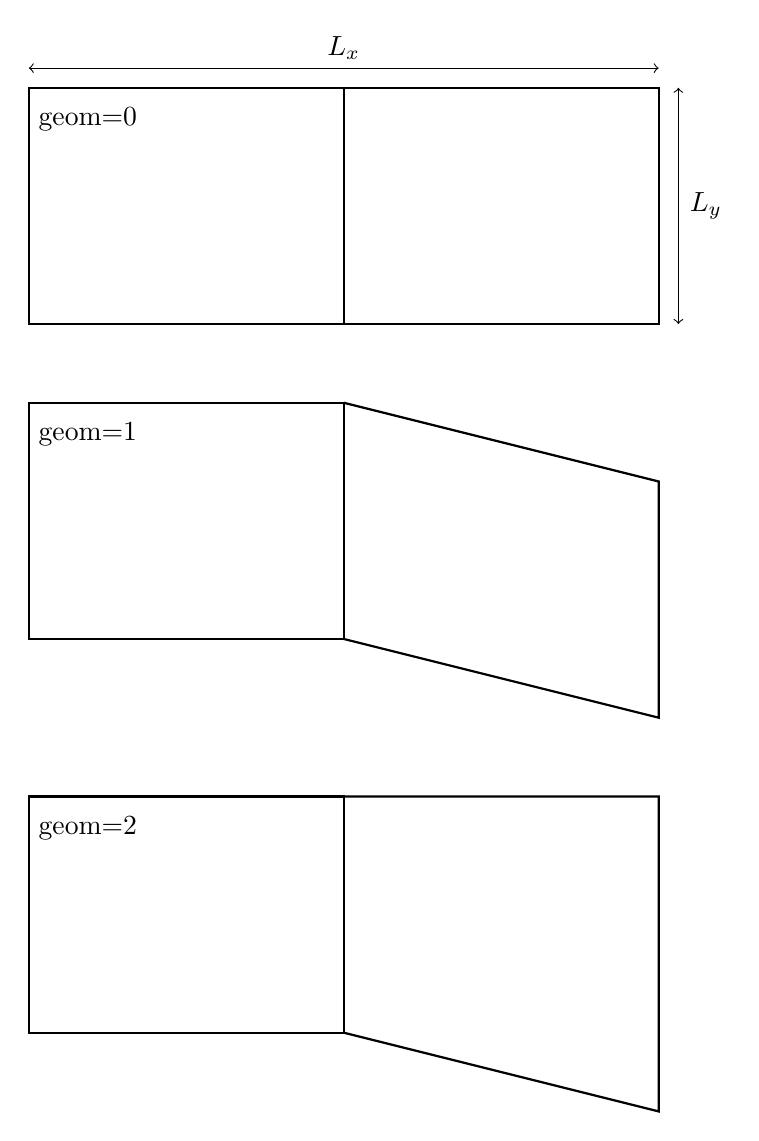
\begin{tikzpicture}
%\draw[step=1cm,gray,very thin] (0,0) grid (10,14); 
\draw[<->,thin] (1,13.25)--(9,13.25);
\node[] at (5,13.5) {$L_x$};
\draw[<->,thin] (9.25,10)--(9.25,13);
\node[] at (9.6,11.5) {$L_y$};
%.............................
\node[] at (1.75,12.6) {geom=$0$};
\draw[thick](1,10) rectangle (5,13); 
\draw[thick](5,10) rectangle (9,13); 
%.............................
\node[] at (1.75,8.6) {geom=$1$};
\draw[thick](1,6) rectangle (5,9);  
\draw[thick](5,6)--(9,5)--(9,8)--(5,9);  
%.............................
\node[] at (1.75,3.6) {geom=$2$};
\draw[thick](1,1) rectangle (5,4);  
\draw[thick](5,1)--(9,0)--(9,4)--(5,4);  
\end{tikzpicture}


\end{center}
and three different elements: ${\bm Q}_1\times P_0$, ${\bm Q}_2\times Q_1$, and ${\bm Q}_3\times Q_2$.

%.............................
\subsubsection{geom=0}

I find that the checkerboard mode is present for the unstable ${\bm Q}_1\times P_0$
element. However, for all three elements the velocity is zero, down to machine precision.
For the two continuous-pressure elements the pressure at the top is 0 and 6 at the 
bottom as expected.

\begin{center}
\includegraphics[width=5.4cm]{python_codes/fieldstone_42/results/geom0/press1}
\includegraphics[width=5.4cm]{python_codes/fieldstone_42/results/geom0/press2}
\includegraphics[width=5.4cm]{python_codes/fieldstone_42/results/geom0/press3}\\
\includegraphics[width=5.4cm]{python_codes/fieldstone_42/results/geom0/vel1}
\includegraphics[width=5.4cm]{python_codes/fieldstone_42/results/geom0/vel2}
\includegraphics[width=5.4cm]{python_codes/fieldstone_42/results/geom0/vel3}\\
{\captionfont From left to right: ${\bm Q}_1\times P_0$, ${\bm Q}_2\times Q_1$, 
and ${\bm Q}_3\times Q_2$.}
\end{center}


%.............................
\subsubsection{geom=1}

We find that the checkerboard mode is now absent and velocities are still zero
for all three elements. The pressure is hydrostatic and only depends on the $y$-coordinate.

\begin{center}
\includegraphics[width=5.1cm]{python_codes/fieldstone_42/results/geom1/press1}
\includegraphics[width=5.1cm]{python_codes/fieldstone_42/results/geom1/press2}
\includegraphics[width=5.1cm]{python_codes/fieldstone_42/results/geom1/press3}\\
\includegraphics[width=5.1cm]{python_codes/fieldstone_42/results/geom1/vel1}
\includegraphics[width=5.1cm]{python_codes/fieldstone_42/results/geom1/vel2}
\includegraphics[width=5.1cm]{python_codes/fieldstone_42/results/geom1/vel3}\\
{\captionfont From left to right: ${\bm Q}_1\times P_0$, ${\bm Q}_2\times Q_1$, 
and ${\bm Q}_3\times Q_2$.}
\end{center}

%.............................
\subsubsection{geom=2}

As in Fortin \& Fortin (1985) we find that the velocity field now showcases 2 ``convection
cells'' for the  ${\bm Q}_1\times P_0$ element (although they have different shapes than 
the ones in their publication) while the velocity remains zero for the other two elements. 

\begin{center}
\includegraphics[width=5.1cm]{python_codes/fieldstone_42/results/geom2/press1}
\includegraphics[width=5.1cm]{python_codes/fieldstone_42/results/geom2/press2}
\includegraphics[width=5.1cm]{python_codes/fieldstone_42/results/geom2/press3}\\
\includegraphics[width=5.1cm]{python_codes/fieldstone_42/results/geom2/vel1}
\includegraphics[width=5.1cm]{python_codes/fieldstone_42/results/geom2/vel2}
\includegraphics[width=5.1cm]{python_codes/fieldstone_42/results/geom2/vel3}\\
{\captionfont From left to right: ${\bm Q}_1\times P_0$, ${\bm Q}_2\times Q_1$, 
and ${\bm Q}_3\times Q_2$.}
\end{center}


On the following figure the root mean square velocity obtained with the 
${\bm Q}_1\times P_0$ element is shown as a function of 
the element size $h$. We find that it decreases quadratically with $h$. 
\begin{center}
\includegraphics[width=6cm]{python_codes/fieldstone_42/results/vrms.pdf}
\end{center}


 %%%%%%%%%%%%%%%%%%%%%%%%%%%%%%%%%%%%%%%%%%%%%%%%%

\newpage %%%%%%%%%%%%%%%%%%%%%%%%%%%%%%%%%%%%%%%%%%%%%%%%%%%%%%%%%%%%%%%%%%%%%%%%%%%%%%%%
\section*{
Stone 43: Time-dependent advection problems
\label{f43}} 
\addcontentsline{toc}{section}{\protect\numberline{} 
Stone 43: Time-dependent advection problems
}
This benchmark originates in \cite{dohu03}. It considers the advection of a product-cosine hill
in a prescribed velocity field. The initial temperature is:
\begin{equation}
T_0(x,y)=
\left\{
\begin{array}{cc}
\frac{1}{4}
\left(1+\cos \pi\frac{x-x_c}{\sigma}\right)
\left(1+\cos \pi\frac{y-y_c}{\sigma}\right)
& \text{if } (x-x_c)^2+(y-y_c)^2\leq \sigma^2 \\
0 & \text{otherwise}
\end{array}
\right.
\end{equation}
The boundary conditions are $T(x,y)=0$ on all four sides of the unit square domain. In what follows we set $x_c=y_c=1/6$ and $\sigma=0.2$.  The velocity field is analytically prescribed: $\vec\upnu=(-(y-y_c),+(x-x_c))$.

In what follows we test the time integration scheme by setting $\alpha_T=1$ (fully implicit formulation), $\alpha=0$ (fully explicit formulation) and $\alpha_T=1/2$ (Crank-Nicolson).  
The timestep is set to $\delta t=2\pi/200$. The density and heat capacity values are set to 1. 
We monitor the minimum and maximum value of the temperature field, as well as the total thermal energy $E_T$ in the system during the 200 time steps ($2\pi$ rotation of the cone):
\[
E_T=\int_\Omega \rho_0 c_p T dV = \int_\Omega T dV = |\Omega| \langle T \rangle 
\qquad
\text{where}
\qquad
\langle T \rangle = \frac{1}{|\Omega|} \int_\Omega T dV
\]
The time evolution of the temperature with the Crank-Nicolson algorithm is shown hereunder:
\begin{center}
a)\includegraphics[width=4.8cm]{python_codes/fieldstone_43/images/crni/velfield}
b)\includegraphics[width=4.8cm]{python_codes/fieldstone_43/images/crni/crnitemp0000}
c)\includegraphics[width=4.8cm]{python_codes/fieldstone_43/images/crni/crnitemp0050}\\
d)\includegraphics[width=4.8cm]{python_codes/fieldstone_43/images/crni/crnitemp0100}
e)\includegraphics[width=4.8cm]{python_codes/fieldstone_43/images/crni/crnitemp0050}
f)\includegraphics[width=4.8cm]{python_codes/fieldstone_43/images/crni/crnitemp0199}\\
{\small a) Velocity field and initial temperature; b,c,d,e,f) Temperature field at timesteps 0,50,100,150,199.} 
\end{center}
Turning now to the statistics, we plot $\min(T)$, $\max(T)$ and $E_T$ as a function of time:
\begin{center}
\includegraphics[width=5cm]{python_codes/fieldstone_43/images/Tmin.pdf}
\includegraphics[width=5cm]{python_codes/fieldstone_43/images/Tmax.pdf}
\includegraphics[width=5cm]{python_codes/fieldstone_43/images/ET.pdf}\\
{\small Time evolution of the min and max temperature and the total energy}
\end{center}
The conclusions are clear: the explicit method diverges quickly and is unusable. The fully implicit and Crank-Nicolson 
method yield similar energy conservation but the fully-implicit showcases a clear loss in maximum temperature as shown in the following figure:
\begin{center}
\includegraphics[width=15cm]{python_codes/fieldstone_43/images/temp}\\
{\small Temperature field after a full rotation with isocontours every 0.1 value.\\ Left: Fully-implicit; Right: Crank-Nicolson}
\end{center}

Finally we can run the experiment (still a $2\pi$ rotation) 
with three different time steps ($\delta t=2\pi/30,2\pi/60,2\pi/120$) 
and we recover very similar results to those presented in \cite{dohu03}:

\begin{center}
\includegraphics[height=8cm]{python_codes/fieldstone_43/images/dohu03}
\includegraphics[height=8cm]{python_codes/fieldstone_43/images/temps_30_60_120}\\
{\small From top to bottom: $\delta t=2\pi/120,2\pi/60,2\pi/30$ with Crank-Nicolson. Left panel is taken from donea \& Huerta \cite{dohu03}}
\end{center}

\begin{center}
\includegraphics[width=5cm]{python_codes/fieldstone_43/images/Tmin_CN.pdf}
\includegraphics[width=5cm]{python_codes/fieldstone_43/images/Tmax_CN.pdf}
\includegraphics[width=5cm]{python_codes/fieldstone_43/images/ET_CN.pdf}\\
{\small Time evolution of the min and max temperature and the total energy obtained with the Crank-Nicolson algorithm for 4 values of the timestep as indicated by the number between parenthesis.}
\end{center}

 %%%%%%%%%%%%%%%%%%%%%%%%%%%%%%%%%%%%%%%%%%%%%%%%%

\newpage %%%%%%%%%%%%%%%%%%%%%%%%%%%%%%%%%%%%%%%%%%%%%%%%%%%%%%%%%%%%%%%%%%%%%%%%%%%%%%%%
\section*{
Stone 44: the flat slab 
\label{f44}} 
\addcontentsline{toc}{section}{\protect\numberline{} 
Stone 44: the flat slab 
}

WORK in PROGRESS

I need a list of nodes on the boundary
I need a GCOORD.txt file with more decimals
I need an even lower resolution  grid
I need the scaling factors for rho,eta, ...


\includegraphics[width=14cm]{python_codes/fieldstone_44/grid_lowres1}\\
\includegraphics[width=7cm]{python_codes/fieldstone_44/grid_lowres2}
\includegraphics[width=7cm]{python_codes/fieldstone_44/grid_lowres3}\\
\includegraphics[width=7cm]{python_codes/fieldstone_44/grid_lowres4}
\includegraphics[width=7cm]{python_codes/fieldstone_44/grid_lowres5}


\begin{center}
\includegraphics[width=14cm]{python_codes/fieldstone_44/sifg19}\\
{\captionfont Taken from \cite{sifg19}}
\end{center}
 %%%%%%%%%%%%%%%%%%%%%%%%%%%%%%%%%%%%%%%%%%%%%%%%%

\newpage %%%%%%%%%%%%%%%%%%%%%%%%%%%%%%%%%%%%%%%%%%%%%%%%%%%%%%%%%%%%%%%%%%%%%%%%%%%%%%%%
\section*{
Stone 45: Rotating cone on a triangular ($P_1$) mesh
\label{f45}} 
\addcontentsline{toc}{section}{\protect\numberline{} 
Stone 45: Rotating cone on a triangular ($P_1$) mesh
}
\lstinputlisting[language=bash,basicstyle=\small]{python_codes/fieldstone_45/keywords}

\begin{center}
Code at \url{https://github.com/cedrict/fieldstone/tree/master/python_codes/fieldstone_45}
\end{center}

\par\noindent\rule{\textwidth}{0.4pt}

%%%%%%%%%%%%%%%%%%%%%%%%%%%%%%%%%%%%%%%%%%%%%%%%%%%%%%%%%%%%%%%%%%%%%%%%%%%%%%%%%%%%%%%%%%%%%%%%%%%%

The domain is a unit square. Only the pure advection equation is solved. 
The setup is identical to Experiment 1 of \stone 43. 
$P_1$ triangular elements are used. A Crank-Nicolson scheme is used for the time
discretisation. The mesh is based on splitting square cells. It is either  
perfectly regular or has some randomness added to it:

\begin{center}
\includegraphics[width=8.5cm]{python_codes/fieldstone_45/results/mesh_reg}
\includegraphics[width=8.5cm]{python_codes/fieldstone_45/results/mesh_rand}\\
{\captionfont Left: regular mesh of 30x30 cells; Right: same, with random noise added}
\end{center}

\begin{center}
\includegraphics[width=5.6cm]{python_codes/fieldstone_45/results/reg0000}
\includegraphics[width=5.6cm]{python_codes/fieldstone_45/results/reg0001}
\includegraphics[width=5.6cm]{python_codes/fieldstone_45/results/reg0002}\\
\includegraphics[width=5.6cm]{python_codes/fieldstone_45/results/reg0003}
\includegraphics[width=5.6cm]{python_codes/fieldstone_45/results/reg0004}
\includegraphics[width=5.6cm]{python_codes/fieldstone_45/results/reg0005}\\
{\captionfont Regular mesh. Temperature field after 0, $2\pi$, $4\pi$, $6\pi$, $8\pi$, $10\pi$ rotation}\\ 
\includegraphics[width=5.6cm]{python_codes/fieldstone_45/results/rand0000}
\includegraphics[width=5.6cm]{python_codes/fieldstone_45/results/rand0001}
\includegraphics[width=5.6cm]{python_codes/fieldstone_45/results/rand0002}\\
\includegraphics[width=5.6cm]{python_codes/fieldstone_45/results/rand0003}
\includegraphics[width=5.6cm]{python_codes/fieldstone_45/results/rand0004}
\includegraphics[width=5.6cm]{python_codes/fieldstone_45/results/rand0005}\\
{\captionfont Randomised mesh. Temperature field after 0, $2\pi$, $4\pi$, $6\pi$, $8\pi$, $10\pi$ rotation} 
\end{center}

\begin{center}
\includegraphics[width=10cm]{python_codes/fieldstone_45/results/T.pdf}\\
{\captionfont Minimum/maximum temperature as a function of time for both grids.} 
\end{center}
 %%%%%%%%%%%%%%%%%%%%%%%%%%%%%%%%%%%%%%%%%%%%%%%%%

\newpage %%%%%%%%%%%%%%%%%%%%%%%%%%%%%%%%%%%%%%%%%%%%%%%%%%%%%%%%%%%%%%%%%%%%%%%%%%%%%%%%
\section*{
Stone 46: MMS1 with Crouzeix-Raviart ($P_2^+\times P_{-1}$) elements  
\label{f46}} 
\addcontentsline{toc}{section}{\protect\numberline{} 
Stone 46: MMS1 with Crouzeix-Raviart ($P_2^+\times P_{-1}$) elements  
}

This stone showcases the Crouzeix-Raviart element (see Section~\ref{sec:crouzeix-raviart})
used to solve the analytical problem "Donea \& Huerta" (see Section~\ref{mms1}).

Out of convenience the pressure is set to zero at location $(x,y)=(1,1)$, so that the 
analytical solution is now $p(x,y)=x(1-x)$. 

\begin{center}
\includegraphics[width=5cm]{python_codes/fieldstone_46/grid}
\includegraphics[width=5cm]{python_codes/fieldstone_46/vel}
\includegraphics[width=5cm]{python_codes/fieldstone_46/press}\\
\includegraphics[width=5cm]{python_codes/fieldstone_46/exx}
\includegraphics[width=5cm]{python_codes/fieldstone_46/exy}
\end{center}

\begin{center}
\includegraphics[width=14cm]{python_codes/fieldstone_46/errors.pdf}
\end{center}

 %%%%%%%%%%%%%%%%%%%%%%%%%%%%%%%%%%%%%%%%%%%%%%%%%

\newpage %%%%%%%%%%%%%%%%%%%%%%%%%%%%%%%%%%%%%%%%%%%%%%%%%%%%%%%%%%%%%%%%%%%%%%%%%%%%%%%%
\section*{
Stone 47: triangular MINI ($P_1^+\times P_1$) element
\label{f47}} 
\addcontentsline{toc}{section}{\protect\numberline{} 
Stone 47: triangular MINI ($P_1^+\times P_1$) element
}
\lstinputlisting[language=bash,basicstyle=\small]{python_codes/fieldstone_47/keywords}

\begin{center}
Code at \url{https://github.com/cedrict/fieldstone/tree/master/python_codes/fieldstone_47}
\end{center}

\par\noindent\rule{\textwidth}{0.4pt}
%%%%%%%%%%%%%%%%%%%%%%%%%%%%%%%%%%%%%%%%%%%%%%%%%%%%%%%%%%%%%%%%%%%%%%%%%%%%%%%%%%%%%%%%%%%%

The domain is a unit cube. Free slip boundary conditions 
The grid is composed of triangles but for simplicity these 
are obtained by splitting rectangles in two, as shown hereunder:

\begin{center}
\includegraphics[width=8cm]{python_codes/fieldstone_47/images/minigrid}\\
Not shown are the nodes for the bubbles in the middle of each triangle. 
\end{center}

This stone showcases the MINI element (see Section~\ref{pair:mini})
used to solve the analytical problem "Donea \& Huerta" (see Section~\ref{mms1}).
Out of convenience the pressure is set to zero at location $(x,y)=(1,1)$, so that the 
analytical solution is now $p(x,y)=x(1-x)$. 

As an experiment I have run convergence tests for two cases: using nqel=3 
quadrature points and using nqel=6 quadrature points.
We find that the velocity and pressure errors converge depend on this crucial
parameter. 
For nqel=3 the velocity and pressure errors converge quadratically and linearly respectively
but for nqel=6 they converge as $h^2$ and $h^{1.5}$ respectively:

\begin{center}
\includegraphics[width=12cm]{python_codes/fieldstone_47/images/reg/errors}
\end{center}

It is worth noticing that although the element is stable, and the error converges
at a respectable rate, the pressure solution is not 'clean': as shown on the 
following figure, there is still some under/overshoot with respect to the analytical solution.

\begin{center}
\includegraphics[width=8cm]{python_codes/fieldstone_47/images/reg/pressure.pdf}
\includegraphics[width=6cm]{python_codes/fieldstone_47/images/rand/press}
\end{center}

Let us now explore the case where the nodes inside the domain are randomly perturbed, i.e. 
a random value  $(\delta_x,\delta_y)\in[-h_x/5,h_x/5]\times[-h_y/5,h_y/5]$ is added 
to their position (while preserving the position of the bubble as the barycenter of each triangle), 
as shown hereunder:

\begin{center}
\includegraphics[width=7cm]{python_codes/fieldstone_47/images/rand/grid}
\includegraphics[width=7cm]{python_codes/fieldstone_47/images/rand/areas}
\end{center}
 
Looking again at the convergence rates of the errors, we see that the velocity errors 
are virtually unchanged but we observe that the pressure errors no more align on a
single line and that the rates are only maintained on average. 

\begin{center}
\includegraphics[width=12cm]{python_codes/fieldstone_47/images/rand/errors}
\end{center}

 %%%%%%%%%%%%%%%%%%%%%%%%%%%%%%%%%%%%%%%%%%%%%%%%%

\newpage %%%%%%%%%%%%%%%%%%%%%%%%%%%%%%%%%%%%%%%%%%%%%%%%%%%%%%%%%%%%%%%%%%%%%%%%%%%%%%%%
\section*{
Stone 48: D\&H with $Q_1\times P_0$, $Q_2\times Q_1$, $Q_3\times Q_2$ and $Q_4\times Q_3$ elements
\label{f48}} 
\addcontentsline{toc}{section}{\protect\numberline{} 
Stone 48: D\&H with $Q_1\times P_0$, $Q_2\times Q_1$, $Q_3\times Q_2$ and $Q_4\times Q_3$ elements
}
In this experiment we consider 4 different finite elements. The idea behind this stone 
is to build a code which code(the FEM build and assembly) is common to all. 
The setup is the Donea \& HUerta benchmark (Section~\ref{mms1}), which has been modified so that 
the pressure is zero at the top right corner.

\begin{verbatim}

Q4xQ3                    Q3xQ2                  Q2xQ1                 Q1Q0

20===21===22===23===24  12====13====14====15  06======07=======08  02===============03
|                    |  |      |     |     |  |        |        |  |                 |
|                    |  |      |     |     |  |        |        |  |                 |
20===21===22===23===24  |      |     |     |  |        |        |  |                 |
|                    |  08====09====10====11  |        |        |  |                 |
|                    |  |      |     |     |  |        |        |  |                 |
20===21===22===23===24  |      |     |     |  03======04=======05  |                 |
|                    |  |      |     |     |  |        |        |  |                 |
|                    |  04====05====06====07  |        |        |  |                 |
20===21===22===23===24  |      |     |     |  |        |        |  |                 |
|                    |  |      |     |     |  |        |        |  |                 |
|                    |  |      |     |     |  |        |        |  |                 |
20===21===22===23===24  00====01====02====03  00======01=======02  00===============01 

12====13=====14=====15  06=======07=======08  02===============03  .=================.
|      |      |      |  |        |         |  |                 |  |                 |
|      |      |      |  |        |         |  |                 |  |                 |
|      |      |      |  |        |         |  |                 |  |                 |
08====09=====10=====11  |        |         |  |                 |  |                 |
|      |      |      |  |        |         |  |                 |  |                 |
|      |      |      |  03=======04=======05  |                 |  |       00        |
|      |      |      |  |        |         |  |                 |  |                 |
04====05=====06=====07  |        |         |  |                 |  |                 |
|      |      |      |  |        |         |  |                 |  |                 |
|      |      |      |  |        |         |  |                 |  |                 |
|      |      |      |  |        |         |  |                 |  |                 |
00====01=====02=====03  00=======01=======02  00===============01  .=================.

mV=25, mP=16            mV=16, mP=9           mV=9, mP=4           mV=4, mP=1      

\end{verbatim}

In the code the 'order' parameter can take values 1,2,3 and 4 which 
correspond to the polynomial order of the velocity approximation ($Q_1$, $Q_2$, $Q_3$ and $Q_4$).

When both nelx and nely values have been chosen, the total number of element 
for a regular 2D grid is simply:
\begin{lstlisting}
nel=nelx*nely
\end{lstlisting}

The number of nodes in each direction is then easily computed:
\begin{lstlisting}
nnx=order*nelx+1 
nny=order*nely+1 
\end{lstlisting}
and so is then the total number of velocity nodes:
\begin{lstlisting}
NV=nnx*nny
\end{lstlisting}

The total number of pressure nodes is as follows:
\begin{lstlisting}
if order==1:
   NP=nelx*nely
if order==2:
   NP=(nelx+1)*(nely+1)
if order==3:
   NP=(2*nelx+1)*(2*nely+1)
if order==4:
   NP=(3*nelx+1)*(3*nely+1)
\end{lstlisting}

Each velocity node has 2 dofs (ndofV=2) while pressure nodes have one dof (ndofP=1) so that 
the size of the blocks and the assembled FE matrix are given by:

\begin{lstlisting}
NfemV=NV*ndofV      
NfemP=NP*ndofP    
Nfem=NfemV+NfemP
\end{lstlisting}

For the linear element, 2 quadrature points per dimension are enough (nqperdim=2), 
while 3 are necessary for the quadratic element (nqperdim=3) and 4 are used  
for the cubic element (nqperdim=4), and 5 for the quartic element,
which can be conveniently implemented as follows:
\begin{lstlisting}
nqperdim=order+1
\end{lstlisting}
The quadrature points location and weight is document in Section~\ref{sec:quadrature}.

Because we wish to use a regular grid, the layout of the points for all three elements 
can be implemented easily:

\begin{lstlisting}
counter=0    
for j in range(0,nny):
    for i in range(0,nnx):
        xV[counter]=i*hx/order
        yV[counter]=j*hy/order
        counter+=1
\end{lstlisting}

The position of the pressure nodes follows a similar logic.

When it comes to the connectivity array, I first started by building it 
for each element as follows:

\begin{lstlisting}
if order==1:
   counter=0
   for j in range(0,nely):
       for i in range(0,nelx):
           iconV[0,counter]=(i)*1+0+(j)*1*nnx+nnx*0 
           iconV[1,counter]=(i)*1+1+(j)*1*nnx+nnx*0 
           iconV[2,counter]=(i)*1+0+(j)*1*nnx+nnx*1 
           iconV[3,counter]=(i)*1+1+(j)*1*nnx+nnx*1 
           counter += 1

if order==2:
   counter = 0
   for j in range(0,nely):
       for i in range(0,nelx):
           iconV[0,counter]=(i)*2+0+(j)*2*nnx+nnx*0 
           iconV[1,counter]=(i)*2+1+(j)*2*nnx+nnx*0 
           iconV[2,counter]=(i)*2+2+(j)*2*nnx+nnx*0 
           iconV[3,counter]=(i)*2+0+(j)*2*nnx+nnx*1 
           iconV[4,counter]=(i)*2+1+(j)*2*nnx+nnx*1 
           iconV[5,counter]=(i)*2+2+(j)*2*nnx+nnx*1 
           iconV[6,counter]=(i)*2+0+(j)*2*nnx+nnx*2 
           iconV[7,counter]=(i)*2+1+(j)*2*nnx+nnx*2
           iconV[8,counter]=(i)*2+2+(j)*2*nnx+nnx*2 
           counter += 1

if order==3:
   counter = 0
   for j in range(0,nely):
       for i in range(0,nelx):
           iconV[ 0,counter]=(i)*3+0+(j)*3*nnx+0*nnx 
           iconV[ 1,counter]=(i)*3+1+(j)*3*nnx+0*nnx 
           iconV[ 2,counter]=(i)*3+2+(j)*3*nnx+0*nnx 
           ...
           iconV[13,counter]=(i)*3+1+(j)*3*nnx+3*nnx 
           iconV[14,counter]=(i)*3+2+(j)*3*nnx+3*nnx 
           iconV[15,counter]=(i)*3+3+(j)*3*nnx+3*nnx 
           counter += 1
\end{lstlisting}
Having done so, it becomes quickly apparent that the connectivity array 
can be computed for all elements as follows:
\begin{lstlisting}
counter=0
for j in range(0,nely):
    for i in range(0,nelx):
        counter2=0
        for k in range(0,order+1):
            for l in range(0,order+1):
                iconV[counter2,counter]=i*order+l+j*order*nnx+nnx*k
                counter2+=1
        counter += 1
\end{lstlisting}
The same approach is taken to build the pressure connectivity array, 
although the $Q_1\times P_0$ element requires special attention since
the pressure is elemental and attributed to a single node inside the element. 

For the other elements I started from:

\begin{lstlisting}
if order==2:
   counter=0
   for j in range(0,nely):
       for i in range(0,nelx):
           iconP[0,counter]=(i)*1+0+(j)*1*(nelx+1)+(nelx+1)*0 
           iconP[1,counter]=(i)*1+1+(j)*1*(nelx+1)+(nelx+1)*0 
           iconP[2,counter]=(i)*1+0+(j)*1*(nelx+1)+(nelx+1)*1 
           iconP[3,counter]=(i)*1+1+(j)*1*(nelx+1)+(nelx+1)*1 
           counter += 1

if order==3:
   counter=0
   for j in range(0,nely):
       for i in range(0,nelx):
           iconP[0,counter]=(i)*2+0+(j)*2*(2*nelx+1)+(2*nelx+1)*0 
           iconP[1,counter]=(i)*2+1+(j)*2*(2*nelx+1)+(2*nelx+1)*0 
           iconP[2,counter]=(i)*2+2+(j)*2*(2*nelx+1)+(2*nelx+1)*0 
           iconP[3,counter]=(i)*2+0+(j)*2*(2*nelx+1)+(2*nelx+1)*1 
           iconP[4,counter]=(i)*2+1+(j)*2*(2*nelx+1)+(2*nelx+1)*1 
           iconP[5,counter]=(i)*2+2+(j)*2*(2*nelx+1)+(2*nelx+1)*1 
           iconP[6,counter]=(i)*2+0+(j)*2*(2*nelx+1)+(2*nelx+1)*2 
           iconP[7,counter]=(i)*2+1+(j)*2*(2*nelx+1)+(2*nelx+1)*2 
           iconP[8,counter]=(i)*2+2+(j)*2*(2*nelx+1)+(2*nelx+1)*2 
           counter += 1

if order==4:
   etc ...
\end{lstlisting}
and quickly arrived at the following compact form:
\begin{lstlisting}
if order>1:
   om1=order-1
   counter=0
   for j in range(0,nely):
       for i in range(0,nelx):
           counter2=0
           for k in range(0,order):
               for l in range(0,order):
                   iconP[counter2,counter]=i*om1+l+j*om1*(om1*nelx+1)+(om1*nelx+1)*k 
                   counter2+=1
           counter += 1
\end{lstlisting}

The core of the code is rather similar if not identical to other stones (i.e.
the loop over elements, the calculation of the elemental matrices, their assembly, 
and the solve).

What is here somewhat elegant is the projection of the pressure field onto the 
velocity grid nodes (mostly for plotting purposes). 
For each element I loop over each velocity node, and evaluate the 
pressure shape function at this location, compute the pressure with it 
and add it in the array q while keeping count of how many 
contributions there are in total per velocity node. 

\begin{lstlisting}
for iel in range(0,nel):
    for i in range(0,mV):
        NNNP[0:mP]=NNP(rVnodes[i],sVnodes[i],order)
        q[iconV[i,iel]]+=np.dot(p[iconP[0:mP,iel]],NNNP[0:mP])
        c[iconV[i,iel]]+=1.

q=q/c
\end{lstlisting}

Finally, since the vtu format does not support higher order elements, I 
here chose to only extract the corner values for each element, 
which translates as follows:
\begin{lstlisting}
vtufile.write("<DataArray type='Int32' Name='connectivity' Format='ascii'> \n")
if order==1:
   for iel in range (0,nel):
       vtufile.write("%d%d%d%d\n" %(iconV[0,iel],iconV[1,iel],iconV[3,iel],iconV[2,iel]))
if order==2:
   for iel in range (0,nel):
       vtufile.write("%d%d%d%d\n" %(iconV[0,iel],iconV[2,iel],iconV[8,iel],iconV[6,iel]))
if order==3:
   for iel in range (0,nel):
       vtufile.write("%d%d%d%d\n" %(iconV[0,iel],iconV[3,iel],iconV[15,iel],iconV[12,iel]))
if order==4:
   for iel in range (0,nel):
       vtufile.write("%d%d%d%d\n" %(iconV[0,iel],iconV[4,iel],iconV[24,iel],iconV[20,iel]))
vtufile.write("</DataArray>\n")
\end{lstlisting}


The following results are obtained by running one of the four scripts {\sl script\_errorsX} 
where X=1,2,3,4. The gnuplot script is to be found in the {\sl images} folder.

The stone implementes two ways of building the FE matrix. When the flag {\sl sparse} 
is false, the $\K$ and $\G$ matrices are built as full arrays, later assembled in a
larger full array, and then only converted to Compressed Sparse Row \index{CSR} before 
it is passed to the solver. When the flag is true, the global FE matrix 
is defined as a {\sl lil\_matrix} (a List of Lists) and it grows in size/memory
every time a new term is added to it. As shown on the following plot, it is about 
twice as slow compared to the first option, but it uses only a fraction of the memory
that the first one does. 

\begin{center}
\includegraphics[height=6.cm]{python_codes/fieldstone_48/images/FEMbuildtimes.pdf}
\end{center}

Also not very surprising: the cost of building the FE matrix increases with the order
of the used elements. A matrix corresponding to 100 $Q_1\times P_0$ elements can be 
built in about 1s, while it will take 7s when $Q_4 \times Q_3$ elements are used. 



%-------------------------------------------------
\subsection*{Results with $Q_1\times P_0$ element}


\begin{center}
\includegraphics[height=6.cm]{python_codes/fieldstone_48/images/q1q0/vel}
\includegraphics[height=6.cm]{python_codes/fieldstone_48/images/q1q0/p}\\
\includegraphics[height=4.cm]{python_codes/fieldstone_48/images/q1q0/pressure.pdf}
\includegraphics[height=4.cm]{python_codes/fieldstone_48/images/q1q0/errors1.pdf}
\end{center}

We see that we recover a second order convergence rate for velocity (as expected) 
but because of the checkerboard pattern the pressure convergence is simply random. 
The smoothed pressure $q$ shows virtually no checkerboard pattern, except on the boundaries.
This is a perfect example for the use of more accurate/clever smoothing procedure, see
Section~\ref{psmoothing}.


\subsection*{Results with $Q_2\times Q_1$ element}

We recover the cubic convergence for the velocity error and the quadratic convergence 
for the pressure:

\begin{center}
\includegraphics[width=8cm]{python_codes/fieldstone_48/images/errors2.pdf}
\end{center}

\subsection*{Results with $Q_3\times Q_2$ element}

The analytical solution is a second order polynomial, which means that the pressure 
shape functions can adequately represent the solution. We recover a fourth-order 
convergence for the velocity error and a superconvergent (fifth order) pressure error 
(but why is it 5th order ?).

\begin{center}
\includegraphics[width=8cm]{python_codes/fieldstone_48/images/errors3.pdf}
\end{center}

\subsection*{Results with $Q_4\times Q_3$ element}

Rather interestingly, now both velocity and pressure analytical solutions 
can be represented exactly by their respective polynomial spaces, so that 
the errors are at machine precision.

\begin{center}
\includegraphics[width=8cm]{python_codes/fieldstone_48/images/errors4.pdf}
\end{center}



 %%%%%%%%%%%%%%%%%%%%%%%%%%%%%%%%%%%%%%%%%%%%%%%%%

\newpage %%%%%%%%%%%%%%%%%%%%%%%%%%%%%%%%%%%%%%%%%%%%%%%%%%%%%%%%%%%%%%%%%%%%%%%%%%%%%%%%
\section*{
Stone 49: Consistent Boundary Flux method on D\&H benchmark with 4 elements 
\label{f49}} 
\addcontentsline{toc}{section}{\protect\numberline{} 
Stone 49: Consistent Boundary Flux method on D\&H benchmark with 4 elements 
}


%----------------------------------------------------
\subsection*{Looking at the four different elements}






%----------------------------------------------------
\subsection*{Looking at the influence of the mas matrix lumping}

 %%%%%%%%%%%%%%%%%%%%%%%%%%%%%%%%%%%%%%%%%%%%%%%%%

\newpage %%%%%%%%%%%%%%%%%%%%%%%%%%%%%%%%%%%%%%%%%%%%%%%%%%%%%%%%%%%%%%%%%%%%%%%%%%%%%%%%
\section*{
Stone 50: Lithosphere extension
\label{f50}} 
\addcontentsline{toc}{section}{\protect\numberline{} 
Stone 50: Lithosphere extension 
}


\includegraphics[width=16cm]{python_codes/fieldstone_50/solution.pdf}

 %%%%%%%%%%%%%%%%%%%%%%%%%%%%%%%%%%%%%%%%%%%%%%%%%

\newpage %%%%%%%%%%%%%%%%%%%%%%%%%%%%%%%%%%%%%%%%%%%%%%%%%%%%%%%%%%%%%%%%%%%%%%%%%%%%%%%%
\section*{
Stone 51: Triangular domain benchmark with MINI element
\label{f51}} 
\addcontentsline{toc}{section}{\protect\numberline{} 
Stone 51: Triangular domain benchmark with MINI element
}
{\sl This fieldstone was developed in collaboration with L. van de Wiel}. 


The following problem is studied in \cite{jolm17}.

The equation to solve are:
\begin{eqnarray}
-\vec{\nabla}p + \Delta \vec{\upnu} + Ra T \vec{e}_y &=& 0\\
\vec\nabla\cdot\vec\upnu &=& 0 \\
-\Delta T + \vec\upnu\cdot\nabla T &=& 0
\end{eqnarray}

The domain is chosen to be the right triangle
with vertices (0,0), (1,0), and (0,1). 
The boundary is considered to be solid walls (no-slip).
For the temperature, a sinusoidal heat source is enforced on the bottom
boundary with a Dirichlet condition ($T(x)=2(1-\cos (2\pi x))$), 
the left wall is set to a constant temperature
of zero, and the hypotenuse wall is perfectly insulated so that a Neumann 
boundary condition is appropriate.

\begin{center}
\includegraphics[width=6cm]{python_codes/fieldstone_51/minigrid5}
\end{center}




 %%%%%%%%%%%%%%%%%%%%%%%%%%%%%%%%%%%%%%%%%%%%%%%%%

\newpage %%%%%%%%%%%%%%%%%%%%%%%%%%%%%%%%%%%%%%%%%%%%%%%%%%%%%%%%%%%%%%%%%%%%%%%%%%%%%%%%
\section*{
Stone 52: Serendipity element in 2D 
\label{f52}} 
\addcontentsline{toc}{section}{\protect\numberline{} 
Stone 52: Serendipity element in 2D
}
In order to test the grid point and connectivity algorithms, 
we use this simple $4\times 3$ element mesh:

\begin{verbatim}

      Q_2 X Q1 (serendipity)                    Q_2 X Q_1 (regular)

15--47--16--48--17--49--18--50--19      54--55--56--57--58--59--60--61--62
 |       |       |       |       |       |   :   |   :   |   :   |   :   |
42      43      44      45      46      45..46..47..48..49..50..51..52..53
 |       |       |       |       |       |   :   |   :   |   :   |   :   |
10--38--11--39--12--40--13--41--14      36--37--38--39--40--41--42--43--44
 |       |       |       |       |       |   :   |   :   |   :   |   :   |
33      34      35      36      37      27..28..29..30..31..32..33..34..35
 |       |       |       |       |       |   :   |   :   |   :   |   :   |
05--29--06--30--07--31--08--32--09      18--19--20--21--22--23--24--25--26
 |       |       |       |       |       |   :   |   :   |   :   |   :   |
24      25      26      27      28      09..10..11..12..13..14..15..16..17
 |       |       |       |       |       |   :   |   :   |   :   |   :   |
00--20--01--21--02--22--03--23--04      00--01--02--03--04--05--06--07--08
\end{verbatim}

We see that the serendipity element-based mesh counts only 51 nodes, as
opposed to 63 for its counterpart.

Setting $nelx=nely$, we can look at the number of velocity nodes for each 
as a function of $nelx$, as shown hereunder:

\begin{center}
\includegraphics[width=6cm]{python_codes/fieldstone_52/NV.pdf}
\includegraphics[width=6cm]{python_codes/fieldstone_52/NV_ratio.pdf}
\end{center}
Looking at the ratio between both, we see that ultimately 
at high resolution, a mesh composed of serendipity elements 
will count 25\% less nodes than a mesh with Taylor-Hood elements.
Since there is not free lunch, what is the price paid in terms of accuracy when using 
the cheaper serendipity? 

The shape functions and their derivatives are in Section~\ref{sec:serendipity2D}.

Although the vtk format does not understand the $Q_2$ element in 2D or 3D, it surprisingly does
understand the serendipity element in 2D (type=23) and 3D (type=25).

\begin{center}
\includegraphics[width=8cm]{python_codes/fieldstone_52/errors.pdf}
\end{center}


 %%%%%%%%%%%%%%%%%%%%%%%%%%%%%%%%%%%%%%%%%%%%%%%%%

\newpage %%%%%%%%%%%%%%%%%%%%%%%%%%%%%%%%%%%%%%%%%%%%%%%%%%%%%%%%%%%%%%%%%%%%%%%%%%%%%%%%
\section*{
Stone 53: the sinking block benchmark 
\label{f53}} 
\addcontentsline{toc}{section}{\protect\numberline{} 
Stone 53: the sinking block benchmark 
}
\url{https://github.com/cedrict/fieldstone/tree/master/python_codes/fieldstone_53}

\vspace{1cm}

This simple benchmark provides challenging numerical experiments 
dealing with large viscosity variations within the simulation
domain. It appears in \cite{gery10} and consists of a bulk of fluid 1 ($\rho_1,\eta_1$)
in which a block of fluid 2 $(\rho_2,\eta_2)$ falls under its own
weight. The domain is a square of size $L_x=L_y=512$km and the
block is initially centred at point ($x=$256 km, $y=$ 384 km) with size
$128\times 128$ km:

\begin{center}
\includegraphics[height=5cm]{python_codes/fieldstone_53/images/setup}
\includegraphics[height=5cm]{python_codes/fieldstone_53/images/vel}\\
{\small Left: setup. Right: velocity field for $\rho_2=3208$, $\eta_1=10^{21}$
and $\eta_2=10^{22}$.}
\end{center}

The simulation is carried out on $32\times32$, $48\times48$ and $64\times 64$ grids. Free slip
boundary conditions are imposed on all sides of the domain. 
In all experiments the density of the surrounding fluid is $\rho_1=3200\text{kg}/\text{m}^3$.
The velocity $v_b$ of the falling block is measured in its centre (note that due to symmetry 
the horizontal component should be zero).

As explained in \cite{thie11}, following physical intuition, one expects 
the velocity $v_b$ of the block to (a) decrease when the viscosity
of the surrounding medium $\eta_1$ increases; (b) increase with the
density contrast $\rho_2-\rho_1$. 
The quantity $v_b \eta_1/(\rho_2-\rho_1)$ is therefore monitored and shown hereunder as a function of 
the viscosity ratio.


\begin{center}
\includegraphics[width=8cm]{python_codes/fieldstone_53/images/results.pdf}\\
{\small
Series of experiments have been conducted with $\rho_2=3208,3232,3328$, 
$\log_{10}(\eta_1)=20,21,22$ and $\log_{10}(\eta_2)=18,18.5,19,...22.5,23,23.5,24$, 
all with 3 mesh resolutions.}
 \end{center}

All experimental points line up on a single curve which further
indicates that the code can deal with gravity driven simulations in the presence
of large viscosity contrasts. These results have been succesfully compared with 
those obtained with ASPECT with the same setup.




 %%%%%%%%%%%%%%%%%%%%%%%%%%%%%%%%%%%%%%%%%%%%%%%%%

\newpage %%%%%%%%%%%%%%%%%%%%%%%%%%%%%%%%%%%%%%%%%%%%%%%%%%%%%%%%%%%%%%%%%%%%%%%%%%%%%%%%
\section*{
Stone 54: ALEs  
\label{f54}} 
\addcontentsline{toc}{section}{\protect\numberline{} 
Stone 54: ALEs 
}
\url{https://github.com/cedrict/fieldstone/tree/master/python_codes/fieldstone_54}

\vspace{1cm}

This stone implements three different free surface/mesh deformation algorithms. 
The first one has all the nodes move with the computed velocity (Lagrangian method)
and is coined 'method 1'. 
The second one ('method 2') only has the top row of nodes moving with the computed velocity, 
while all the nodes underneath are static (this is obviously not a viable method for 
large deformations). 
The third one ('method 3') is the method used in ASPECT and described in Rose et al (2017) \cite{robh17}.
Its implementation is described in Section~\ref{sec:freesurface}.

%...........................................................
\subsubsection*{Experiment 1 - relaxation of topography}

The domain is a 2D Cartesian box of size 512$\times$512km, with free slip on left, 
bottom and right sides, free surface at the top. 
Mantle material characterised by $\rho_m=3200$ and $\eta_m=10^{22}$. 
Gravity is vertical and Earth like. 
The surface is perturbed at startup by $\delta y = A \cos (\pi x /L_x)$ with $A$=1km.
200 time steps with $\delta t=10$kyr are carried out.
The root mean square velocity, the total volume of the domain, the min/max elevation
values of the surface are recorded over time. 

\begin{center}
\includegraphics[width=7.5cm]{python_codes/fieldstone_54/images/exp1/u}
\includegraphics[width=7.5cm]{python_codes/fieldstone_54/images/exp1/v}\\
{\scriptsize velocity field at $t=0$ with resolution 24x24}
\end{center}

The results hereunder are obtained for all three methods at two different resolutions (16x16 
and 24x24 elements).
The plots on the left column are obtained with the movement of the top nodes being constrained in 
the vertical direction, while the plots on the right column are obtained with nodes being 
allowed to move in both $x$ and $y$ directions (note that for method 3 the normals are not -yet-
computed with the method of Eq. 49 in \cite{robh17} but instead by a simple geometric rule).

\begin{center}
a) \includegraphics[width=7cm]{python_codes/fieldstone_54/images/exp1/elevation_vert.pdf}
   \includegraphics[width=7cm]{python_codes/fieldstone_54/images/exp1/elevation_full.pdf}\\
b) \includegraphics[width=7cm]{python_codes/fieldstone_54/images/exp1/elevation_log_vert.pdf}
   \includegraphics[width=7cm]{python_codes/fieldstone_54/images/exp1/elevation_log_full.pdf}\\
c) \includegraphics[width=7cm]{python_codes/fieldstone_54/images/exp1/volume_vert.pdf}
   \includegraphics[width=7cm]{python_codes/fieldstone_54/images/exp1/volume_full.pdf}\\
d) \includegraphics[width=7cm]{python_codes/fieldstone_54/images/exp1/vrms_vert.pdf}
   \includegraphics[width=7cm]{python_codes/fieldstone_54/images/exp1/vrms_full.pdf}\\
e) \includegraphics[width=7cm]{python_codes/fieldstone_54/images/exp1/surface_topography_200_vert.pdf}
   \includegraphics[width=7cm]{python_codes/fieldstone_54/images/exp1/surface_topography_200_full.pdf}\\
{\scriptsize 
a) min/max of free surface topo as a function of time; 
b) free surface topo maximum (in log scale) as a function of time; 
c) measured volume of the domain with numerical quadrature normalised by the expected volume $L_xL_y$;
d) root mean square velocity as a function of time;
e) final elevation at the 200th time step.}
\end{center}

%...........................................................
\subsubsection*{Experiment 2,3 - extension}

We now consider a rectangular domain (crust sized) of $128\times32$km, discretised by means of $40\times10$ elements.
The fluid is identical to the one above and so is gravity. 
Extensional boundary conditions are applied. In the first case, a 1cm/yr horizontal velocity is applied on both sides, while in the second case a 2cm/yr velocity is applied on the right while 0 is prescribed to the left. Free slip conditions are otherwise prescribed on the sides and bottom. 100 time steps are carried out with $\delta t=10^4$yr. Only method 3 is used here.

\begin{center}
\includegraphics[width=13cm]{python_codes/fieldstone_54/images/exp2-3/vel0}\\
{\scriptsize Velocity field for both experiments at $t=0$.}
\end{center}


Despite the asymmetry in the boundary conditions, we expect the same evolution of the domain geometry. This is indeed what we recover with surprising accuracy. 'vert' stands for only vertical movement allowed (i.e. $n_x=0$, 
$n_y=1$) while 'both dir' stands for the use of dynamically computed normal vectors (based on geometrical consideration).

\begin{center}
\includegraphics[width=7cm]{python_codes/fieldstone_54/images/exp2-3/volume.pdf}
\includegraphics[width=7cm]{python_codes/fieldstone_54/images/exp2-3/surface.pdf}\\
{\scriptsize Left: time evolution of the normalised volume for both boundary condition types; Right: surface at the end of the simulation.}
\end{center}


\begin{center}
\includegraphics[width=7cm]{python_codes/fieldstone_54/images/exp2-3/vrms.pdf}
\includegraphics[width=7cm]{python_codes/fieldstone_54/images/exp2-3/elevation.pdf}\\
{\scriptsize Left: Root mean square velocity as a function of time; Right: time evolution of the elevation (min and max virtually indistinguishable).} 
\end{center}


%...........................................................
\subsubsection*{Experiment 4,5 - extension with bottom inflow}

This is the same setup as above, but we now impose an influx boundary condition at the bottom: $v=0.5cm$ (this balances the outflux exactly) and 
the horizontal component at the bottom is set to the left value (-1 or 0 cm/yr) for $x\leq L_x/2$ and to the right value +1 or +2 cm/yr for $x\geq L_x/2$.

\begin{center}
\includegraphics[width=7cm]{python_codes/fieldstone_54/images/exp4-5/volume.pdf}
\includegraphics[width=7cm]{python_codes/fieldstone_54/images/exp4-5/surface.pdf}\\
\includegraphics[width=7cm]{python_codes/fieldstone_54/images/exp4-5/vrms.pdf}
\includegraphics[width=7cm]{python_codes/fieldstone_54/images/exp4-5/elevation.pdf}\\
\end{center}

We can conclude that the 'vertical movement only' conserves volume/mass better and the free surface remains symmetrical unless the full normal is used which is simply explained by having $\vec{v}\cdot\vec{n}$ as a boundary condition: in the asymmetric extension case, the velocity is always to the right while the normal has an $x$ component which is negative and positive, therefore introducing an asymmetry in the surface boundary conditions.

\begin{center}
\includegraphics[width=9cm]{python_codes/fieldstone_54/images/exp4-5/v}\\
{\scriptsize Top to bottom: 
symmetric extension, full normal vector; 
symmetric extension, vertical normal vector; 
asymmetric extension, full normal vector; 
asymmetric extension, vertical normal vector}
\end{center}

%...........................................................
\subsubsection*{Experiment 6 - pure advection test}

\begin{center}
\includegraphics[width=7cm]{python_codes/fieldstone_54/images/exp6/velp}\\
\includegraphics[width=7cm]{python_codes/fieldstone_54/images/exp6/surface.pdf}
\includegraphics[width=7cm]{python_codes/fieldstone_54/images/exp6/elevation.pdf}\\
{\scriptsize Results after 100 time steps = 1Myr}
\end{center}

%...........................................................
\subsubsection*{Experiment 7 - pure advection test of a cosine bump}

The initial topography bump is given by
\[
y(x)=A \left[ 1+ \cos \left( \frac{x-x_0}{w} \pi \right) \right]
\]
with $A=1000$m, $x_0=0.345678L_x$ and $w=$15km. This is a somewhat ideal case 
since the transition from flat to bump is very smooth.

The viscosity is set to $10^{26}$Pa$\cdot$s so that the velocity of the 
viscous relaxation of the topography is negligible with regards to the advection velocity
(+1cm/yr on left and right boundaries). I also choose a resolution of 80x20 elements.

\begin{center}
\includegraphics[width=8cm]{python_codes/fieldstone_54/images/exp7/v}
\end{center}

If only the vertical normal is used then {\sl nothing} moves since the 
velocity is always perpendicular to the normal. 

What follows is obtained when the full normal is used. 
After 20 timesteps the topography has been advected and we already observe some 
visible asymmetry (and oscillations) on the surface:
\begin{center}
\includegraphics[width=11cm]{python_codes/fieldstone_54/images/exp7/surface.pdf}
\end{center}

On the following plots the left column shows $(\vec{\upnu}\cdot \vec{n})n_x$ 
as a function of the $x$-coordinate and the 
right column shows $(\vec{\upnu}\cdot \vec{n})n_y$, both for timesteps 1,2,3,5,10,20. 
Both quantities form the 
boundary conditions for the mesh deformation.  
Since I have chosen $x_0$ such that it does not fall on a node, the initial 
topography is {\sl not} symmetric and therefore the normal vectors at the nodes 
on the left and right of the peak are not identical. From the second timestep (the first one 
for which the free surface algo uses a non zero Stokes velocity as boundary condition)
we see that both components $(\vec{\upnu}\cdot \vec{n})n_x$ and $(\vec{\upnu}\cdot \vec{n})n_y$ are asymmetric! 


\begin{center}
\includegraphics[width=6cm]{python_codes/fieldstone_54/images/exp7/n_dov_v_nx_001.pdf}
\includegraphics[width=6cm]{python_codes/fieldstone_54/images/exp7/n_dov_v_ny_001.pdf}\\
\includegraphics[width=6cm]{python_codes/fieldstone_54/images/exp7/n_dov_v_nx_002.pdf}
\includegraphics[width=6cm]{python_codes/fieldstone_54/images/exp7/n_dov_v_ny_002.pdf}\\
\includegraphics[width=6cm]{python_codes/fieldstone_54/images/exp7/n_dov_v_nx_003.pdf}
\includegraphics[width=6cm]{python_codes/fieldstone_54/images/exp7/n_dov_v_ny_003.pdf}\\
\includegraphics[width=6cm]{python_codes/fieldstone_54/images/exp7/n_dov_v_nx_005.pdf}
\includegraphics[width=6cm]{python_codes/fieldstone_54/images/exp7/n_dov_v_ny_005.pdf}\\
\includegraphics[width=6cm]{python_codes/fieldstone_54/images/exp7/n_dov_v_nx_010.pdf}
\includegraphics[width=6cm]{python_codes/fieldstone_54/images/exp7/n_dov_v_ny_010.pdf}\\
\includegraphics[width=6cm]{python_codes/fieldstone_54/images/exp7/n_dov_v_nx_020.pdf}
\includegraphics[width=6cm]{python_codes/fieldstone_54/images/exp7/n_dov_v_ny_020.pdf}
\end{center}

The inescapable conclusion is that the algorithm (as it is now implemented with the normal 
vector) is incapable of advecting a bump. 

{\bf NEW}: In what follows, the Stokes system is solved once, and the obtained velocity
is used to compute the mesh velocity boundary condition for the Laplace system. 
The resolution is set to 100x25. I have implemented the $L_2$ projection approach 
of \cite{robh17} for both Q1 and Q2 elements. For such a smooth topography the 
Q1 and geometrical approach (i.e. using geometrically computed normal vectors) are
very similar although Q1 produces tiny undershoots. Q2 however generates oscillations
which makes the computed velocity not suited as a boundary condition to move surface nodes. 

From left to right: horizontal component, vertical component, and vector form 
of the computed mesh velocity bc.

\begin{center}
\includegraphics[width=7cm]{python_codes/fieldstone_54/images/exp7/100x25/umesh}
\includegraphics[width=7cm]{python_codes/fieldstone_54/images/exp7/100x25/vmesh}\\
\includegraphics[width=11cm]{python_codes/fieldstone_54/images/exp7/100x25/velmesh}
\end{center}

I haven't used any of the projections to carry out timestepping.

%......................................................................
\subsubsection*{Experiment 8 - pure advection test of a pyramidal bump}

This is a nearly identical experiment as the previous one, but now the bump is 
composed of two straight lines, of slopes $\pm 0.1$.
Pyramid centered at $x=0.345678L_x$, of half width 15km. $\rho=3000$, $\eta=10^{26}$.
Resolution 60x15. +1cm/yr prescribed on left and right. dt=10kyr. 

\begin{center}
\includegraphics[width=9cm]{python_codes/fieldstone_54/images/exp8/v}
\end{center}

\begin{center}
\includegraphics[width=8cm]{python_codes/fieldstone_54/images/exp8/surface.pdf}\\
\includegraphics[width=10cm]{python_codes/fieldstone_54/images/exp8/bc_vmesh.pdf}
\end{center}

Results are not crazy bad, but we should be able to do better ... the pyramid 
becomes more and more deformed after only 20km of advection (but surprisingly retains its height). 



{\bf NEW}: In what follows, the Stokes system is solved once, and the obtained velocity
is used to compute the mesh velocity boundary condition for the Laplace system. 
The resolution is set to 100x25. I have implemented the $L_2$ projection approach 
of \cite{robh17} for both Q1 and Q2 elements. For such a broken line topography the 
geometrical approach (i.e. using geometrically computed normal vectors) is better.
Q1 and Q2 both produce under/overshoots/oscillations with no clear winner. 

From left to right: horizontal component, vertical component, and vector form 
of the computed mesh velocity bc.

\begin{center}
\includegraphics[width=7cm]{python_codes/fieldstone_54/images/exp8/100x25/umesh}
\includegraphics[width=7cm]{python_codes/fieldstone_54/images/exp8/100x25/vmesh}\\
\includegraphics[width=11cm]{python_codes/fieldstone_54/images/exp8/100x25/velmesh}
\end{center}

I haven't used any of the projections to carry out timestepping.

%......................................................................


%......................................................................
\subsubsection*{Experiment 9 - Rayleigh-Taylor instability}

The setup is as follows:
\begin{center}
\includegraphics[width=5cm]{python_codes/fieldstone_54/images/exp9/robh17}
\end{center}
The sinusoidal perturbation is given by 
\[
y(x)=400e3 - 500 \cos( 2 \pi x /L_x)
\]

Because I do not have compositional fields or markers implemented in this code I have 
to align the mesh with the initial sinusoidal perturbation and run the model in 
Lagrangian mode. Also, as shown in \cite{kamm10}, this experiment is prone to drunken sailor 
instabilities and I have therefore fixed dt=1000yr.
As a consequence, the model will run until elements become too distorted. 

\begin{center}
\includegraphics[width=8cm]{python_codes/fieldstone_54/images/exp9/surface}
\end{center}




 %%%%%%%%%%%%%%%%%%%%%%%%%%%%%%%%%%%%%%%%%%%%%%%%%

\newpage %%%%%%%%%%%%%%%%%%%%%%%%%%%%%%%%%%%%%%%%%%%%%%%%%%%%%%%%%%%%%%%%%%%%%%%%%%%%%%%%
\section*{
Stone 55: Subduction as a thin-sheet problem  
\label{f55}} 
\addcontentsline{toc}{section}{\protect\numberline{} 
Stone 55: Subduction as a thin-sheet problem  
}
\lstinputlisting[language=bash,basicstyle=\small]{python_codes/fieldstone_55/keywords}

\url{https://github.com/cedrict/fieldstone/tree/master/python_codes/fieldstone_55}

\begin{mdframed}[backgroundcolor=red!5]
This stone was partially contributed by E. van der Wiel.
\end{mdframed}

\index{contributors}{E. van der Wiel}


\vspace{1cm}

Parameters for the setup are defined in {\sl parameters.py}.
This file is used in {\sl generate\_nodes.py} which produces the
{\sl subd.node} file which contains the coordinates of all key points 
on the boundary of the domain and along the material interfaces.
This file is then further processed by the triangle 
program\footnote{\url{https://www.cs.cmu.edu/~quake/triangle.html}}
as follows:
\begin{verbatim}
./triangle -q -a200000000 -o2 subd.node
\end{verbatim}
The '-q' option adds vertices to the mesh to
ensure that all angles are between 20 and 140 degrees. 
The '-a' makes sure that no triangle has an area larger than 
the supplied number. The '-o2' generates a mesh composed 
of second order triangles (six nodes per element, rather than three) and the
three extra nodes of an element fall at the midpoints of the three edges.
This generates two files: 'subd.1.ele' which contains the connectivity 
of all generated triangles and 'subd.1.node' which contains the coordinates
of all nodal points. 
These two files are then read in {\sl fieldstone.py} and stored in the xV, yV and iconV arrays.

Gravity is vertical and Earth-like. Free-slip boundary conditions are imposed on the top while 
the other boundaries are free (in/outflow determined freely based on the internal dynamics). 
In order to remove the horizontal null space the average horizontal velocity is set to zero. 
Crouzeix-Raviart elements are used, see Section~\ref{sec:crouzeix-raviart}.
The density of the mantle is set to zero while the subducting plate has a density $\delta\rho$. 

\begin{center}
\includegraphics[width=7.5cm]{python_codes/fieldstone_55/images/mesh}
\includegraphics[width=7.5cm]{python_codes/fieldstone_55/images/area}\\
\includegraphics[width=7.5cm]{python_codes/fieldstone_55/images/u}
\includegraphics[width=7.5cm]{python_codes/fieldstone_55/images/v}\\
\includegraphics[width=7.5cm]{python_codes/fieldstone_55/images/sr}
\includegraphics[width=7.5cm]{python_codes/fieldstone_55/images/press}\\
\includegraphics[width=7.5cm]{python_codes/fieldstone_55/images/rho}
\includegraphics[width=7.5cm]{python_codes/fieldstone_55/images/eta}\\
{\captionfont Mesh composed of 31,765 triangles.
Other parameters: $\theta_0=60\degree$, $\eta_1=10^{21}$, $\gamma=100$, 
$L_x$=3000km, $L_y$=1500km, $\delta\rho=100$, $L=$400km, $h=$100km, $d=$50km. 
Note that the bottom boundary is open.}
\end{center}

%\begin{center}
%\includegraphics[width=5cm]{python_codes/fieldstone_55/images/spine_u}
%\includegraphics[width=5cm]{python_codes/fieldstone_55/images/spine_v}
%\includegraphics[width=5cm]{python_codes/fieldstone_55/images/spine_vel}\\
%{\scriptsize horizontal and vertical velocity, and velocity norm as a function 
%of $s$. $s$ is measured from 
%left to right on the midsurface and excludes the rounded edges of the slab.}
%\end{center}

We have also run this model with ASPECT for the case where free slip 
boundary conditions are prescribed on all sides. 
Velocities on the midsurface are reported hereunder alongside those
obtained with fieldstone and the BEM method.

\begin{center}
\includegraphics[width=7.5cm]{python_codes/fieldstone_55/images/u_midsurface}
\includegraphics[width=7.5cm]{python_codes/fieldstone_55/images/v_midsurface}\\
\includegraphics[width=7.5cm]{python_codes/fieldstone_55/images/u_perimeter}
\includegraphics[width=7.5cm]{python_codes/fieldstone_55/images/v_perimeter}\\
{\captionfont Top row: midsurface velocity measurements. Bottom row: slab/plate perimeter 
velocity measurements. 'open' means no b.c. on sides and bottom; 'f.s. sides' means 
free slip b.c. on left and right sides, open at the bottom; 'f.s. all' means 
free slip b.c. on sides and bottom.}
\end{center}

\newpage
Finally, we have run this experiment over time with ASPECT (unfortunately viscosities were 100 times 
too small so that the times should be multiplied by 100):
\begin{center}
\includegraphics[width=5.26cm]{python_codes/fieldstone_55/images/aspect/grid_comp0000}
\includegraphics[width=5.26cm]{python_codes/fieldstone_55/images/aspect/grid_comp0090}
\includegraphics[width=5.26cm]{python_codes/fieldstone_55/images/aspect/grid_comp0180}\\
\includegraphics[width=5.26cm]{python_codes/fieldstone_55/images/aspect/vel_sr0000}
\includegraphics[width=5.26cm]{python_codes/fieldstone_55/images/aspect/vel_sr0090}
\includegraphics[width=5.26cm]{python_codes/fieldstone_55/images/aspect/vel_sr0180}\\
{\captionfont Left: t=0, middle t=64kyr, right: t=100kyr.}
\end{center}


\begin{center}
\includegraphics[width=11cm]{python_codes/fieldstone_55/images/mid_evolution}\\
{\captionfont Time evolution of the midline of the slab.}
\end{center}


\begin{center}
\includegraphics[width=14cm]{python_codes/fieldstone_55/images/meshes}
\end{center}

%area = 2*0.537071*h**2 + (7*h)*h , 80728764230.49994 with h=100km

\vspace{3cm}

%\begin{center}
%\includegraphics[width=7cm]{python_codes/fieldstone_55/images/spine_Us}
%\includegraphics[width=7cm]{python_codes/fieldstone_55/images/spine_Ws}\\
%{\scriptsize Parallel and perpendicular velocity to midsurface. $s$ is measured from 
%left to right on the midsurface and excludes the rounded edges of the slab.}
%\end{center}


Literature: \cite{fogm14}
 %%%%%%%%%%%%%%%%%%%%%%%%%%%%%%%%%%%%%%%%%%%%%%%%%

\newpage %%%%%%%%%%%%%%%%%%%%%%%%%%%%%%%%%%%%%%%%%%%%%%%%%%%%%%%%%%%%%%%%%%%%%%%%%%%%%%%%
\section*{
Stone 56: Dynamics of the Salt Water - Fresh Water Interface
\label{f56}} 
\addcontentsline{toc}{section}{\protect\numberline{} 
Stone 56: Dynamics of the Salt Water - Fresh Water Interface  
}

Saltwater intrusion in coastal aquifers is a world wide observable phenomena. The mixing of salt and fresh water reduces groundwater quality. It potentially threatens the usability as drinking water. Extensive pumping causing a decrease of groundwater levels amplifies this effect. 


Gravity drives salty sea water land inward due to its higher density if an aquifer's water table is lower than sea level.
An interface develops between salt and fresh water, which is stable due to the density difference. Along the interface slight mixing occurs due to diffusion.
As for most processes in nature, coupled partial differential equations describe the movement of the interface between salt and fresh water. 

The target of this exercise is to model a simplified form of the process. Basic assumption hereby are: (i) groundwater flow is mostly horizontal (called {\sl Depuit assumption}); 
(ii) the salt and fresh water interface is sharp, meaning we neglect mixing due to dispersion and diffusion. 


We investigate a portion of an aquifer of length $L$ and depth $H$. Within the aquifer, an interface separates salt water and fresh water as illustrated here under:

\begin{center}
\includegraphics[width=13cm]{python_codes/fieldstone_56/images/setup}
\end{center}

The interface~$h(x,t)$ is a function of the horizontal location~$x$ and time~$t$. 
For simplicity, we assume an aquifer thickness of $H=1$. Thus, the values for the position of the interface as a function in the $z$ direction range between zero and one: $h(x,t) \in [0,1]$.

The differential equation describing the movement of the interface $h(x,t)$ is given by 

\begin{equation} \label{eq:01}
	\frac{\partial h(x,t)}{\partial t} = \Gamma \frac{\partial}{\partial x} \left( \frac{ h(1-h)\partial h / \partial x}{1+(\partial h/\partial x)^2} \right)
\end{equation}

The constant $\Gamma=\frac{\kappa }{ \mu g (\rho_{ \rm salt}-\rho_{\rm fresh})}$ summarizes the physical properties: of the aquifer (permeability $\kappa$), of the fluids (viscosity $\mu$, density of salt water~$\rho_{\rm salt}$ and density of fresh water~$\rho_{\rm fresh}$) and the gravity constant $g$.

The differential equation has the character of a non-linear diffusion equation with a non-constant diffusion coefficient $D(h)$:

\begin{equation} \label{eq:02}
	\frac{\partial h}{\partial t} = \Gamma \frac{\partial}{\partial x} \left( D(h)  \frac{ \partial h}{\partial x} \right)
	\quad \quad D(h(x,t)) = \frac{ h(1-h)}{1+(\partial h/\partial x)^2}
\end{equation}

According to the value range of $h \in [0,1]$, $D$ has the property of $D(0)=D(1)=0$ (this differential equation is therefore called {\sl degenerate}). \index{stones}{Degenerate Diffusion Equation}

Despite the complexity of the initial differential equation, an analytical solution can be postulated in the form of:
\begin{equation}  \label{eq:04}
	h(x,t) = a(t)\cdot x + 0.5
\end{equation}

The interface $h$ is a linear function in $x$ with a time-dependent slope~$a(t)$. It rotates with time around the fix point~$(0;0.5)$. 
The slope~$a(t)$ can be determined by the ordinary differential equation (REF??):
\begin{equation}  \label{eq:05}
\frac{ da(t) }{dt} = - \frac{2a^3}{1+a^2}
\end{equation}

The value range of $a$ is limited to $0<a(t)<1$ corresponding to a maximal slope angle of $45^\circ$. The differential equation in $a(t)$ has an implicit solution:
\begin{equation} \label{eq:05b}
t = \frac 1 2 \ln \left( \frac{a(0)}{a(t)} \right) + \frac 1 4 \left( \frac{1}{a(t)^2} - \frac{1}{a(0)^2} \right)
\end{equation}

We aim to implement a numerical solution of the differential equation 1 which allows us to calculate the location of the interface $h(x,t)$ at specified locations $x$ and times $t$.

{\Huge To Do} in 2D only



 %%%%%%%%%%%%%%%%%%%%%%%%%%%%%%%%%%%%%%%%%%%%%%%%%

\newpage %%%%%%%%%%%%%%%%%%%%%%%%%%%%%%%%%%%%%%%%%%%%%%%%%%%%%%%%%%%%%%%%%%%%%%%%%%%%%%%%
\section*{
Stone 57: DG-FEM: 1D steady state diffusion
\label{f57}} 
\addcontentsline{toc}{section}{\protect\numberline{} 
Stone 57: DG-FEM: 1D steady state diffusion
}
\lstinputlisting[language=bash,basicstyle=\small]{python_codes/fieldstone_57/keywords}

\url{https://github.com/cedrict/fieldstone/tree/master/python_codes/fieldstone_57}

We follow the discretisation presented in Section~\ref{ss:dgss1D} and use the 
successive substitution to arrive at the solution. 
Let us start by fixing ${\cal E}=4$ and ${\cal C}=0$ and setting the absolute convergence 
tolerance to $10^{-8}$.

\begin{center}
\includegraphics[width=8cm]{python_codes/fieldstone_57/results/E04_C000/convergence.pdf}
\end{center}

\begin{center}
\includegraphics[width=7cm]{python_codes/fieldstone_57/results/E04_C000/T_minus_evol.pdf}
\includegraphics[width=7cm]{python_codes/fieldstone_57/results/E04_C000/q_minus_evol.pdf}
\end{center}

%...................................................
\paragraph{Effect of resolution} Keeping the same parameters we see that the 
number of required iterations to convergence increases linearly with the number of elements.

\begin{center}
\begin{tabular}{cc}
\hline
nelx & \# iterations \\
\hline
08 &60  \\
16 &116 \\
32 &220 \\
64 &436 \\
128 & 857 \\
\hline
\end{tabular}
\end{center}

%...................................................
\paragraph{Effect of ${\cal E}$ \& ${\cal C}$ values} 
We now keep nelx=32 and explore the effect of these parameters on the 
required number of iterations:

\begin{center}
\begin{tabular}{ccc}
\hline
${\cal E}$ & ${\cal C}$ & \# iterations \\
\hline
1& 0 & 772 \\
2& 0 & 414 \\
3& -0.5 & {\bf 104} \\
3& 0    & 284 \\
3& 0.5 & 129 \\
4&-1/2& 196 \\
4&0   & 220 \\
4&+1/2& 196 \\
5& -1/2 & 256 \\
5& 0 & 195 \\
5& +1/2 & 256 \\
6& 0 & 246 \\
10& 0 & 486 \\
\hline
\end{tabular}
\end{center}

\begin{center}
${\cal E}=4$ \& ${\cal C}=-1/2$  \hspace{2cm}
${\cal E}=4$ \& ${\cal C}=0$ \hspace{2cm}
${\cal E}=4$ \& ${\cal C}=+1/2$\\
\includegraphics[width=5cm]{python_codes/fieldstone_57/results/E04_Cm0p5/convergence.pdf}
\includegraphics[width=5cm]{python_codes/fieldstone_57/results/E04_C000/convergence.pdf}
\includegraphics[width=5cm]{python_codes/fieldstone_57/results/E04_Cp0p5/convergence.pdf}\\
{\captionfont Using ${\cal C}\neq 0$ yields a very linear convergence.}
\end{center}


\begin{center}
${\cal E}=4$ \& ${\cal C}=-1/2$  \hspace{2cm}
${\cal E}=4$ \& ${\cal C}=0$ \hspace{2cm}
${\cal E}=4$ \& ${\cal C}=+1/2$\\
\includegraphics[width=5cm]{python_codes/fieldstone_57/results/E04_Cm0p5/error.pdf}
\includegraphics[width=5cm]{python_codes/fieldstone_57/results/E04_C000/error.pdf}
\includegraphics[width=5cm]{python_codes/fieldstone_57/results/E04_Cp0p5/error.pdf}\\
{\captionfont Error between computed and analytical solution as a function of $x$} 
\end{center}


\begin{center}
${\cal E}=4$ \& ${\cal C}=-1/2$  \hspace{2cm}
${\cal E}=4$ \& ${\cal C}=0$ \hspace{2cm}
${\cal E}=4$ \& ${\cal C}=+1/2$\\
\includegraphics[width=5cm]{python_codes/fieldstone_57/results/E04_Cm0p5/T_minus_evol}
\includegraphics[width=5cm]{python_codes/fieldstone_57/results/E04_C000/T_minus_evol}
\includegraphics[width=5cm]{python_codes/fieldstone_57/results/E04_Cp0p5/T_minus_evol}\\
\includegraphics[width=5cm]{python_codes/fieldstone_57/results/E04_Cm0p5/q_minus_evol}
\includegraphics[width=5cm]{python_codes/fieldstone_57/results/E04_C000/q_minus_evol}
\includegraphics[width=5cm]{python_codes/fieldstone_57/results/E04_Cp0p5/q_minus_evol}\\
{\captionfont The path to a converged solution is quite different for the three values 
of ${\cal C}$ tested.} 
\end{center}




 %%%%%%%%%%%%%%%%%%%%%%%%%%%%%%%%%%%%%%%%%%%%%%%%%

\newpage %%%%%%%%%%%%%%%%%%%%%%%%%%%%%%%%%%%%%%%%%%%%%%%%%%%%%%%%%%%%%%%%%%%%%%%%%%%%%%%%
\section*{
Stone 60: DG-FEM: 1D advection 
\label{f60}} 
\addcontentsline{toc}{section}{\protect\numberline{} 
Stone 60: DG-FEM: 1D advection 
}
\lstinputlisting[language=bash,basicstyle=\small]{python_codes/fieldstone_60/keywords}

This stone implements the 1D discontinuous Galerkin method to solve the simple 
advection equation:
\[
\frac{\partial T}{\partial t} + u \frac{\partial T}{\partial x} = 0
\]




%---------------------------------------------
\subsection*{The code}

The mesh counts {\tt nelx} linear elements and therefore {\tt nnx} nodes.

The timestep is determined by means of the CFL condition:
\begin{lstlisting}
dt=C*hx/u
\end{lstlisting}
The mesh is very simply built:
\begin{lstlisting}
x=np.linspace(0,Lx,nnx)
\end{lstlisting}
We need to declare four arrays: the nodal temperature both on the left and 
on the right of each node, and their memory of the previous time step. 
\begin{lstlisting}
T_minus=np.zeros(nnx,dtype=np.float64)      
T_minus_old=np.zeros(nnx,dtype=np.float64)  
T_plus=np.zeros(nnx,dtype=np.float64)       
T_plus_old=np.zeros(nnx,dtype=np.float64)   
\end{lstlisting}
Initial temperatures are then prescribed on both {\tt T\_plus} 
and $T\_minus$ arrays, and then copied to the 'old' arrays.

We then enter the time stepping loop:
\begin{lstlisting}
for istep in range(0,nstep):
\end{lstlisting}
At each timestep the boundary conditions are reapplied\footnote{It is a bit weird that 
we prescribe a temperature b.c. on a node with an outflow...?}:
\begin{lstlisting}
T_minus[0]=T_left
T_plus[0]=T_left
T_minus[nnx-1]=T_right
T_plus[nnx-1]=T_right
\end{lstlisting}
We then loop over all elements:
\begin{lstlisting}
for iel in range(0,nel):
\end{lstlisting}
and compute the corresponding $k$ and $k+1$ values:
\begin{lstlisting}
k=iel
kp1=iel+1
\end{lstlisting}
The $T^+$ and $T^-$ fields are then updated following Eq.~\eqref{eq:dgadv5}:
\begin{lstlisting}
T_plus[k]   =T_plus_old[k]   +C*(-3*T_plus_old[k]-T_minus_old[k+1]+4*T_minus[k])
T_minus[k+1]=T_minus_old[k+1]+C*( 3*T_plus_old[k]-T_minus_old[k+1]-2*T_minus[k])
\end{lstlisting}







%---------------------------------------------
\subsection*{Results}

%---------------------------------------------
\subsubsection*{Experiment 1}

We consider the following advection problem taken from Li \cite[ex 5.2]{li06}.
It is also carried out in \stone~43.

The domain has dimension $L_x=1$. 
The temperature is prescribed on the left and the right boundary to be zero. 
The initial temperature is given by
\[
T(x,0)=
\left\{
\begin{array}{ll}
\sin (10 \pi x) & \textrm{for } x< 0.1 \\
0               & \textrm{for } x\geq 0.1 
\end{array}
\right.
\]
The velocity is set to $u=0.1$.
We use 200 elements and a time step of $\delta t=10^{-4}$. 
We run the model to time $t=8$ so we need 80,000 time stpes. 

Note that the CFL-number is then very small: 
\[
C = \frac{\delta t \cdot u}{h} = \frac{10^{-4} \cdot  0.1}{1/200} = 0.002
\]

\begin{center}
\includegraphics[width=9cm]{python_codes/fieldstone_60/results/exp1/T.pdf}\\
{\captionfont Temperature field at three different times.}
\end{center}

\todo[inline]{redo with standard Galerkin and compare!}

%---------------------------------------------
\subsubsection*{Experiment 2}

This advection benchmark originates in Donea \& Huerta \cite{dohu03}
and it also to be found in Thieulot (2011) \cite{thie11} (and in 
Section~\ref{ss:appAthie11}).

The domain has dimension $L_x=1$. 
The temperature is prescribed on the left at $T=1$
and the right boundary at $T=0$.
The initial temperature is given by
\[
T(x,0)=
\left\{
\begin{array}{ll}
1 & \textrm{for } x< 0.25 \\
0 & \textrm{for } x\geq 0.1 
\end{array}
\right.
\]
Velocity is set to $u=1$, the number of elements to 50 ($h=0.02$), the CFL number to 0.1 (
so $\delta t=0.002$), and the number of time steps to 250, so that we expect the front
to be at $x=3L_x/4$.  

\begin{center}
\includegraphics[width=8cm]{python_codes/fieldstone_60/results/exp2/T.pdf}\\
\includegraphics[width=8cm]{images/supg/fantom3}\\
{\captionfont Left: Temperature field at different times; 
Right: Taken and modified from Thieulot (2011) \cite{thie11}}
\end{center}

It is rather surprising that the DG results are so much worse than the SG results (even without 
SUPG stabilisation).









 %%%%%%%%%%%%%%%%%%%%%%%%%%%%%%%%%%%%%%%%%%%%%%%%%

\newpage %%%%%%%%%%%%%%%%%%%%%%%%%%%%%%%%%%%%%%%%%%%%%%%%%%%%%%%%%%%%%%%%%%%%%%%%%%%%%%%%
\section*{
Stone 79: DG-FEM: 2D steady state diffusion
\label{f79}}
\addcontentsline{toc}{section}{\protect\numberline{} 
Stone 79: DG-FEM: 2D steady state diffusion
}
\lstinputlisting[language=bash,basicstyle=\small]{python_codes/fieldstone_79/keywords}

\begin{center}
Code at \url{https://github.com/cedrict/fieldstone/tree/master/python_codes/fieldstone_79}
\end{center}

\par\noindent\rule{\textwidth}{0.4pt}

{\sl This stone was developed in collaboration with Jort Jansen}. \index{contributors}{J. Jansen}

\par\noindent\rule{\textwidth}{0.4pt}

%%%%%%%%%%%%%%%%%%%%%%%%%%%%%%%%%%%%%%%%%%%%%%%%%%%%%%%%%%%%%%%%%%%%%%%%%%%%%%%%%%%%%%%%

Before reading what follows I urge you to go to Chapter~\ref{dgfem}. The derivations 
presented therein are long and complex, but absolutely necessary to make sense of the code.  
The code has been written for both bilinear ($Q_1$) quadrilateral elements and 
and linear ($P_1$) triangular elements. Meshes are then as follows:

\begin{center}
\includegraphics[width=10cm]{python_codes/fieldstone_79/images/grids2D_tris}\\
{\captionfont Example of a 4x3 triangular mesh.}
\end{center}

\begin{center}
\includegraphics[width=10cm]{python_codes/fieldstone_79/images/grids2D_quads}\\
{\captionfont Example of a 4x3 quadrilateral mesh.}
\end{center}

Contrarily to standard continuous finite elements nodes/vertices are not 
shared across elements so that the node layout is entirely based on the 
already built connectivity array {\tt icon}. Node coordinates are stored in 
{\tt xT} and {\tt yT}.

Six ascii output files are opened at the beginning of the code, and in these 
various statistics will be written out. These are 
{\sl T\_stats.ascii}, {\sl qx\_stats.ascii}, {\sl qy\_stats.ascii},
{\sl residual\_T\_stats.ascii}, {\sl residual\_qx\_stats.ascii}, and {\sl residual\_qy\_stats.ascii}.

Then a large number of arrays is declared. Then contain information that is needed 
when building the matrices and vectors later on and it is convenient to store this information
beforehand. They all start with {\tt edge} and record the normal to the edge, its center coordinates, 
its length, whether it is on the domain boundary, etc ... Because this is an educative code 
with a simple mesh topology we can directly ascribe the normals to each side. If a mesher, like 
Triangle \cite{shew14}, was used then we would need to compute the normals to each side by means
of simple geometrical considerations.

We continue to build the necessary arrays pertaining to neighbours. 
We build the {\tt edgeX\_neighb[iel]} arrays which contain the identity of the element 
on the other size of edge X of element iel.
For instance, looking at the example above of a triangular mesh, we have
\begin{lstlisting}
edge1_neighb[0]=-1
edge2_neighb[0]=1
edge3_neighb[0]=-1
...
edge1_neighb[10]=3
edge2_neighb[10]=11
edge3_neighb[10]=9
\end{lstlisting}
where the -1 value indicates that there is no element neighbour.

We then build the arrays {\tt edgeX\_neighbedge[iel]} (where X stand for 1, 2, 3, 
or 4) which stores the identity/number of the edge on the element across the common face
(if there is a neighbour).
For instance:
\begin{lstlisting}
edge1_neighbedge[10]=2
edge2_neighbedge[10]=3
edge3_neighbedge[10]=1
\end{lstlisting}


\begin{center}
\includegraphics[width=10cm]{python_codes/fieldstone_79/images/drawing}\\
{\captionfont When two triangles are neighbours (here along edge 1
of grey triangle) three configurations can occur.}
\end{center}





%............................
\paragraph{Iterative process}
Although we are solving the steady-state diffusion equation, we still need to carry out 
iterations (this is a consequence of the DG formulation itself and it is not the 
case for 'regular' finite elements).
These iterations are implemented as follows:
\begin{lstlisting}
for iter in range(0,niter):
\end{lstlisting}
where {\tt niter} is set to 100. Vector residuals are computed for $T$, $q_x$ and $q_y$. When the
infinite-norm of all three is below the tolerance {\tt tol} then the system is considered 
converged and iterations are stopped.   
For each iteration the code prints a number of helpful statistics in the terminal:
\begin{scriptsize}
\begin{verbatim}
iter=   0 : T,qx,qy (m/M)= 6.944e-03 2.053e+00 | -1.067e+01 2.054e+01 | -1.067e+01 2.054e+01 | max(resT)= 5.700e-01 (tol= 1.0e-09)
iter=   1 : T,qx,qy (m/M)= 9.982e-04 2.053e+00 | -3.991e+00 8.163e+00 | -3.991e+00 8.163e+00 | max(resT)= 7.515e-01 (tol= 1.0e-09)
iter=   2 : T,qx,qy (m/M)= 9.982e-04 2.702e+00 | -2.278e+00 3.863e+00 | -2.278e+00 3.863e+00 | max(resT)= 5.316e-01 (tol= 1.0e-09)
...
iter=  41 : T,qx,qy (m/M)= 3.473e-13 2.000e+00 | 1.000e+00 1.000e+00 | 1.000e+00 1.000e+00 | max(resT)= 1.537e-09 (tol= 1.0e-09)
iter=  42 : T,qx,qy (m/M)= 3.473e-13 2.000e+00 | 1.000e+00 1.000e+00 | 1.000e+00 1.000e+00 | max(resT)= 9.357e-10 (tol= 1.0e-09)
\end{verbatim}
\end{scriptsize}

Each iteration consists in a sweep through elements and we implement a forward-backward scheme:
even-numbered iterations got from 0 to nel-1, while odd-numbered ones go from nel-1 down to 0:
\begin{lstlisting}
if iter%2==0:
   start=0
   end=nel
   step=1
else:
   start=nel-1
   end=-1
   step=-1
\end{lstlisting}





\newpage

Explore/implement

source term
randomised nodes so no right angles




%------------------------------
\subsubsection*{Benchmark \#1} 

We define the simple temperature field 
\[
T(x,y)=x+y
\]
over a unit square domain, so that (taking $k=1$) we have
\[
q_x(x,y)=-1
\qquad
q_y(x,y)=-1
\]
I prescribe this temperature on all four sides of the domain. 


VERIFY: minus sign problem for heat fluxes ?


%------------------------------
\subsubsection*{Benchmark \#2} 
 %%%%%%%%%%%%%%%%%%%%%%%%%%%%%%%%%%%%%%%%%%%%%%%%%

\newpage %%%%%%%%%%%%%%%%%%%%%%%%%%%%%%%%%%%%%%%%%%%%%%%%%%%%%%%%%%%%%%%%%%%%%%%%%%%%%%%%
\section*{
Stone 58: Elastic disk under compression
\label{f58}} 
\addcontentsline{toc}{section}{\protect\numberline{} 
Stone 58: Elastic disk under compression
}
\lstinputlisting[language=bash,basicstyle=\small]{python_codes/fieldstone_58/keywords}

\noindent \Literature:
\begin{itemize}
\item Compaction creep of sands due to time-dependent grain failure: Effects of chemical environment,
      applied stress, and grain size. Brzesowsky \etal{} (2014) \cite{brhb14}
\item Failure behavior of single sand grains: Theory versus experiment. Brzesowsky \etal{} (2011) \cite{brsp11}
\item Time-independent compaction behavior of quartz sands. Brzesowsky \etal{} (2014) \cite{brsp14}
\item Determination of the tensile strength of rock by a compression test of an 
      irregular test piece. Hiramatsu \etal{} (1966) \cite{hiok66}
\item Micromechanics of sand grain failure and sand compaction. Brzesowsky (1995) \cite{brze95}
\item Contact fatigue in silica sand—Observations and modeling. Wang \& Michalowski (2015) \cite{wami15}
\item Tensile stress concentration and compressive failure in cemented granular material. 
      Wong \& Wu (1995)\cite{wowu95}
\item Micromechanics of pressure-induced grain crushing in porous rocks. Zhang \etal{} (1990) \cite{zhwd90}
\end{itemize}

%----------------------------
\subsubsection*{Experiment 1}

This benchmark is well document in \cite{sadd14}.
%what follows is from the book itself
Let us investigate the solution to the plane problem shown hereunder of a circular disk 
loaded by equal but opposite concentrated forces along a given diameter. 
This particular problem is of special interest since this geometry is used 
in standard testing of bituminous and other brittle materials such as 
concrete, asphalt, rock, and ceramics. Normally referred to as the Brazilian or indirect tension test, 
the sample and loading geometry create a tension zone along the loaded diameter, 
thus allowing determination of the tensile strength of the specimen material. 
Standard direct tension testing on such brittle materials has led to difficulty 
in establishing a failure region in the sample’s central interior away from 
the gripping locations.

\begin{center}
\includegraphics[width=5cm]{python_codes/fieldstone_58/experiment1/setup}\\
{\captionfont Setup of the experiment.}
\end{center}

The mesh is regular and made of concentric layers of triangles. The original algorithm
which was used in \elefant was written by L. van Wiel.  Given the nature of the boundary 
conditions we wish to apply we make sure that two faces are present at the top and bottom 
locations of the disc, which is why the mesh is rotated 90\degree 
after it is generated. \index{contributors}{L. van de Wiel} 

The mesh is composed of {\tt nsection} sections (must be an even number)
as shown hereunder (for {\tt nLayers}=3). 
\begin{center}
\includegraphics[width=5cm]{python_codes/fieldstone_58/images/mesh4}
\includegraphics[width=5cm]{python_codes/fieldstone_58/images/mesh6}
\includegraphics[width=5cm]{python_codes/fieldstone_58/images/mesh8}\\
{\captionfont Mesh composed of 4 sections (left), 6 sections (middle) and 8 sections (right).}
\end{center}

The pressure $P$ prescribed at $y=\pm R$ is actually given by $P \delta({\bm r_\pm})$. 
From \cite{sadd14} (example 8.10, p209), the stress solution is given by:

\begin{eqnarray}
\sigma_{xx}(x,y)&=& -\frac{2P}{\pi}\left[\frac{(R-y)x^2}{r_1^4} + \frac{(R+y)x^2}{r_2^4} -\frac{1}{D} \right] \\
\sigma_{yy}(x,y)&=& -\frac{2P}{\pi}\left[\frac{(R-y)^3}{r_1^4} + \frac{(R+y)^3}{r_2^4} -\frac{1}{D} \right] \\
\sigma_{xy}(x,y)&=&  \frac{2P}{\pi}\left[\frac{(R-y)^2 x}{r_1^4} - \frac{(R+y)^2x}{r_2^4}  \right]
\end{eqnarray}
where 
\[
r_1=\sqrt{x^2 + (R-y)^2}
\quad\quad
r_2=\sqrt{x^2 + (R+y)^2}
\]

The pressure is given by:
\begin{eqnarray}
p(x,y) 
&=& -\frac{1}{2}(\sigma_{xx} + \sigma_{yy}) \nonumber\\
&=& 
 \frac{P}{\pi} \left[ \frac{(R-y)x^2}{r_1^4} + \frac{(R+y)x^2}{r_2^4} -\frac{1}{D} \right] 
+ \frac{P}{\pi} \left[ \frac{(R-y)^3}{r_1^4} + \frac{(R+y)^3}{r_2^4} -\frac{1}{D} \right] \\
&=& 
\frac{P}{\pi} \left[ \frac{(R-y)x^2 + (R-y)^3 }{r_1^4} + \frac{(R+y)x^2 + (R+y)^3}{r_2^4} - \frac{2}{D}\right] 
\end{eqnarray}

On the $x$-axis ($y=0$) these results simplify to give
\begin{eqnarray}
\sigma_{xx}(x,0) &=& \frac{2P}{\pi D} \left( \frac{D^2-4x^2}{D^2+4x^2}  \right)^2 \\
\sigma_{yy}(x,0) &=& -\frac{2P}{\pi D} \left( \frac{4D^4}{(D^2+4x^2)^2} -1 \right) \\
\sigma_{xy}(x,0) &=& 0 \\
p(x,0) 
&=& \frac{P}{\pi} \left[ \frac{(R-y)x^2 + (R-y)^3 }{r_1^4} + \frac{(R+y)x^2 + (R+y)^3  }{r_2^4}  - \frac{2}{D} \right] \\
&=& \frac{P}{\pi} \left[ \frac{Rx^2 + R^3 }{(x^2+R^2)^2} + \frac{Rx^2 + R^3  }{(x^2+R^2)^2}  - \frac{2}{D} \right] \\
&=& \frac{2P}{\pi} \left[ \frac{R(x^2 + R^2 )}{(x^2+R^2)^2} - \frac{1}{D} \right] \\
&=& \frac{2P}{\pi} \left[ \frac{R }{x^2+R^2} - \frac{1}{D} \right] \\
\end{eqnarray}

On the $y$-axis ($x=0$) the stresses are 
\begin{eqnarray}
\sigma_{xx}(0,y) &=& \frac{2P}{\pi D} \\
\sigma_{yy}(0,y) 
&=& -\frac{2P}{\pi} \left( \frac{2}{D-2y} + \frac{2}{D+2y} -\frac{1}{D} \right) \\
&=& -\frac{2P}{\pi} \left( \frac{1}{R-y} + \frac{1}{R+y} -\frac{1}{D} \right) \\
\sigma_{xy} (0,y) &=& 0 \\
p(0,y) 
&=& \frac{P}{\pi} \left[ \frac{(R-y)^3 }{(R-y)^4} + \frac{ (R+y)^3  }{(R+y)^4}  - \frac{2}{D} \right] \\
&=& \frac{P}{\pi} \left[ \frac{1}{R-y} + \frac{ 1 }{R+y}  - \frac{2}{D} \right] 
\end{eqnarray}
In the code the pressure is retrieved after the displacements are computed. 
In 2D, we have (using Eq.~\ref{eq:twoELAST} for the stress tensor):
\begin{eqnarray}
p
&=& -\frac{1}{2}(\sigma_{xx} + \sigma_{yy}) \nonumber\\
&=& -\frac{1}{2} \left[
\lambda (\varepsilon_{xx}+\varepsilon_{yy}) + 2 \mu \varepsilon_{xx} +
\lambda (\varepsilon_{xx}+\varepsilon_{yy}) + 2 \mu \varepsilon_{yy} 
\right] \\
&=& -\frac{1}{2} \left[
2\lambda (\varepsilon_{xx}+\varepsilon_{yy}) + 2 \mu (\varepsilon_{xx} + \varepsilon_{yy} \right]\nn\\
&=& -(\lambda+\mu) (\varepsilon_{xx}+\varepsilon_{yy}) 
\end{eqnarray}

The radius is set to $R=1$, and the disc is centered on the origin. The disc 
is discretised by means of {\sl nlayers} concentric layers of $P_1$ triangles.
I set $\mu=1$ and $\nu=0.25$. 

The boundary conditions are as follows: on the two vertical edges at $y=R$ and $y=-R$ 
the pressure is applied. Furthermore because of the symmetry of the problem, 
and in order to remove the expected nullspaces in the displacement field, 
we fix $u=0$ on the vertical axis and $v=0$ on the horizontal axis.
In the coming plots the number of layers (which needs to be odd) is varied, from 31 to 111.
Note that the displacement is not analytically known but the computed displacement 
nicely converge to a single smooth curve.

\begin{center}
\begin{tabular}{lrrrr}
\hline
{\tt nlayers} & {\tt NV} & {\tt nel} & {\tt Nfem} & $v_{rms}$\\
\hline
\hline
21  &  1387 &  2646 &  2774 & 1.043847e-01\\ 
31  &  2977 &  5766 &  5954 & 1.049944e-01\\
41  &  5167 & 10086 & 10334 & 1.052457e-01\\
51  &  7957 & 15606 & 15914 & 1.053750e-01\\
61  & 11347 & 22326 & 22694 & 1.054509e-01\\
71  & 15337 & 30246 & 30674 & 1.054994e-01\\
81  & 19927 & 39366 & 39854 & 1.055324e-01\\
91  & 25117 & 49686 & 50234 & 1.055560e-01\\
101 & 30907 & 61206 & 61814 & 1.055735e-01\\
111 & 37297 & 73926 & 74594 & 1.055868e-01\\
\hline
\end{tabular}

\includegraphics[width=8cm]{python_codes/fieldstone_58/experiment1/vrms}
\end{center}


\newpage
\begin{center}
a)\includegraphics[width=7.3cm]{python_codes/fieldstone_58/experiment1/press_xaxis.pdf}
b)\includegraphics[width=7.3cm]{python_codes/fieldstone_58/experiment1/press_yaxis.pdf}\\
c)\includegraphics[width=7.3cm]{python_codes/fieldstone_58/experiment1/sigmaxx_xaxis.pdf}
d)\includegraphics[width=7.3cm]{python_codes/fieldstone_58/experiment1/sigmaxx_yaxis.pdf}\\
e)\includegraphics[width=7.3cm]{python_codes/fieldstone_58/experiment1/sigmayy_xaxis.pdf}
f)\includegraphics[width=7.3cm]{python_codes/fieldstone_58/experiment1/sigmayy_yaxis.pdf}\\
g)\includegraphics[width=7.3cm]{python_codes/fieldstone_58/experiment1/sigmaxy_xaxis.pdf}
h)\includegraphics[width=7.3cm]{python_codes/fieldstone_58/experiment1/sigmaxy_yaxis.pdf}\\
i)\includegraphics[width=7.3cm]{python_codes/fieldstone_58/experiment1/u_xaxis.pdf}
j)\includegraphics[width=7.3cm]{python_codes/fieldstone_58/experiment1/v_yaxis.pdf}\\
{\captionfont a,b) pressure along the $x$-axis;
c,d) $\sigma_{xx}$  along the $x-$ and $y-$axis; 
e,f) $\sigma_{yy}$  along the $x-$ and $y-$axis; 
g,h) $\sigma_{xy}$  along the $x-$ and $y-$axis; 
i) horizontal displacement along the $x-$axis; 
j) vertical displacement along the $y-$axis}
\end{center}

\newpage
\begin{center}
\includegraphics[width=5.4cm]{python_codes/fieldstone_58/experiment1/111/u}
\includegraphics[width=5.4cm]{python_codes/fieldstone_58/experiment1/111/v}
\includegraphics[width=5.4cm]{python_codes/fieldstone_58/experiment1/111/divv}\\
\includegraphics[width=5.4cm]{python_codes/fieldstone_58/experiment1/111/p}
\includegraphics[width=5.4cm]{python_codes/fieldstone_58/experiment1/111/q}
\includegraphics[width=5.4cm]{python_codes/fieldstone_58/experiment1/111/e}\\
\includegraphics[width=5.4cm]{python_codes/fieldstone_58/experiment1/111/exx}
\includegraphics[width=5.4cm]{python_codes/fieldstone_58/experiment1/111/eyy}
\includegraphics[width=5.4cm]{python_codes/fieldstone_58/experiment1/111/exy}\\
\includegraphics[width=5.4cm]{python_codes/fieldstone_58/experiment1/111/sigma_xx}
\includegraphics[width=5.4cm]{python_codes/fieldstone_58/experiment1/111/sigma_yy}
\includegraphics[width=5.4cm]{python_codes/fieldstone_58/experiment1/111/sigma_xy}\\
{\captionfont Results for nLayers=11}
\end{center}

\newpage

\begin{center}
a)\includegraphics[width=8cm]{python_codes/fieldstone_58/experiment1/contours}
b)\includegraphics[width=5cm]{python_codes/fieldstone_58/experiment1/111/e_2}\\
{\captionfont 
a) Maximum shear stress contours and corresponding photoelastic isochromatic 
for a disk under diametrical compression \cite{sadd14};\\
b) computed second invariant of the strain tensor.}
\end{center}


We can also look at the principal stresses.
The principal direction angle $\theta_p$ defines the principal
directions where the only stresses are normal stresses, and 
is given by the relationship:
\[
\tan (2\theta_p) =  \frac{2 \sigma_{xy}}{\sigma_{xx} -\sigma_{yy}}
\]
The principal stresses are found from the original stresses via
 \[
\sigma_{1,2}=\frac{\sigma_{xx}+\sigma_{yy}}{2} \pm \sqrt{  \left(\frac{\sigma_{xx}-\sigma_{yy}}{2}\right)^2 +\sigma_{xy}^2 }
 \]



\newpage
%----------------------------
\subsubsection*{Experiment 2}

This experiment was designed in collaboration with T. Shinohara \index{contributors}{T. Shinohara}. 
Unlike the previous one it does not have an analytical solution. Ideally we wished to look at a 
cluster of grains as shown hereunder. However, because of the symmetries of the problem we can 
here again only model one grain, with (idealised) boundary conditions:
 
\begin{center}
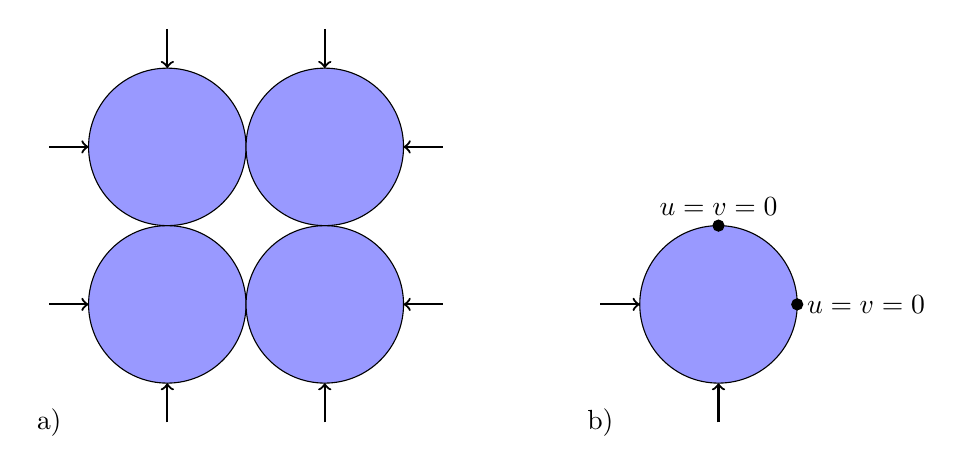
\begin{tikzpicture}
%\draw[fill=gray!23,gray!23](0,0) rectangle (11,6);
%\draw[step=0.5cm,gray,very thin] (0,0) grid (11,6); %background grid
\filldraw[fill=blue!40!white, draw=black] (2,2) circle (1cm);
\filldraw[fill=blue!40!white, draw=black] (4,2) circle (1cm);
\filldraw[fill=blue!40!white, draw=black] (2,4) circle (1cm);
\filldraw[fill=blue!40!white, draw=black] (4,4) circle (1cm);
\draw[thick,->] (0.5,2) -- (1,2); \draw[thick,->] (5.5,2) -- (5,2);
\draw[thick,->] (0.5,4) -- (1,4); \draw[thick,->] (5.5,4) -- (5,4);
\draw[thick,->] (2,0.5) -- (2,1); \draw[thick,->] (2,5.5) -- (2,5);
\draw[thick,->] (4,0.5) -- (4,1); \draw[thick,->] (4,5.5) -- (4,5);
\draw[thick,->] (7.5,2) -- (8,2);
\draw[thick,->] (9,0.5) -- (9,1); 
\filldraw[fill=blue!40!white, draw=black] (9,2) circle (1cm);
\filldraw[black] (10,2) circle (2pt) node[anchor=west] {$u=v=0$};
\filldraw[black] (9,3) circle (2pt) node[anchor=south] {$u=v=0$};
\node[] at (0.5,0.5)   {a)};
\node[] at (7.5,0.5)   {b)};
\end{tikzpicture}\\
{\captionfont a) assembly of four circular grains and the pressure boundary conditions; 
b) simplified setup of a single grain.}
\end{center}

\begin{center}
\includegraphics[width=5.5cm]{python_codes/fieldstone_58/experiment2/displ}
\includegraphics[width=5.5cm]{python_codes/fieldstone_58/experiment2/displx}
\includegraphics[width=5.5cm]{python_codes/fieldstone_58/experiment2/disply}\\
\includegraphics[width=5.5cm]{python_codes/fieldstone_58/experiment2/divv}
\includegraphics[width=5.5cm]{python_codes/fieldstone_58/experiment2/p}
\includegraphics[width=5.5cm]{python_codes/fieldstone_58/experiment2/strain}\\
\includegraphics[width=10cm]{python_codes/fieldstone_58/experiment2/dispvect}
\end{center}






 %%%%%%%%%%%%%%%%%%%%%%%%%%%%%%%%%%%%%%%%%%%%%%%%%

\newpage %%%%%%%%%%%%%%%%%%%%%%%%%%%%%%%%%%%%%%%%%%%%%%%%%%%%%%%%%%%%%%%%%%%%%%%%%%%%%%%%
\section*{
Stone 59: Flow Down an Inclined Plane 
\label{f59}} 
\addcontentsline{toc}{section}{\protect\numberline{} 
Stone 59: Flow Down an Inclined Plane
}

\lstinputlisting[language=bash,basicstyle=\small]{python_codes/fieldstone_59/keywords}

\begin{center}
\includegraphics[width=5cm]{python_codes/fieldstone_59/images/setup}\\
{\captionfont REDO with tikz}
\end{center}

\paragraph{Linear viscous fluid}

We start from the Stokes equation for isoviscous fluids:
\[
\eta \Delta \vec{\upnu} - \vec\nabla p + \rho \vec{g} = \vec{\bm 0}
\]
Assuming that the fluid is incompressible and that the incline is infinite, 
then $\vec{\upnu}=(u(y),0)$.
The $x$-component of the equation then writes:
\[
\eta\left(\frac{\partial^2 u}{\partial x^2}+\frac{\partial^2 u}{\partial y^2} \right)
- \frac{\partial p}{\partial x} + \rho g_x =0
\]
\[
\Rightarrow \qquad 
\eta\frac{\partial^2 u}{\partial y^2} 
+ \rho g \sin\alpha =0
\]
since $\partial_x\rightarrow 0$.
This 2nd order ODE can be integrated twice. The two integration constants are 
determined by setting $u(y=0)=0$ (no slip) and the shear stress to be zero at the (free)
surface. The velocity profile is given by:
\[
u(y)=\frac{\rho g \sin \alpha}{2 \eta} (2h-y)y
\]
We can now compute the components of the strain rate tensor:
\[
\dot{\varepsilon}_{xx}=0
\qquad
\qquad
\dot{\varepsilon}_{yy}=0
\qquad
\qquad
\dot{\varepsilon}_{xy}
=\frac{1}{2} \left( \frac{\partial u}{\partial y} + \frac{\partial v}{\partial x} \right)
=\frac{1}{2} \frac{\partial u}{\partial y} 
= \frac{\rho g \sin \alpha}{2 \eta} (h-y)
\]

We now make the assumption that this problem is a very simplified ice sheet flow problem.
The angle $\alpha$ is typically small and for $\alpha\sim 0.5-1$\degree, then $\sin\alpha\sim 0.01$. 
We also have $\rho\sim1000$, $g\sim$10,  $h\sim2500$ and we postulate the 
ice viscosity to be $\eta\sim 10^m$,.
The velocity is maximum at the surface and is given by
\begin{equation}
u(y=h)=
\frac{\rho g \sin \alpha}{2 \eta}h^2 
\sim \frac{1000 \cdot 10 \cdot 0.01}{ 2\cdot 10^m}2500^2
\sim 3\cdot 10^{8-m}
\label{eq:ice1}
\end{equation}

\begin{center}
\includegraphics[height=9cm]{python_codes/fieldstone_59/images/neem}
\includegraphics[height=9cm]{python_codes/fieldstone_59/images/narh15}\\
{\captionfont Ice velocity map (magnitude, in logarithmic scale) of the Greenland Ice Sheet
derived from SAR data of the Sentinel-1A satellite, acquired in Interferometric Wide Swath
Mode (IW) between January and March 2015. Taken from \cite{narh15}.}
\end{center}

As shown on the figures above the typical ice sheet velocity values around the NEEM ice core 
is $\sim 0.03m/day \simeq 3\cdot 10^{-7}$m/s. 
Then, in order for the top of the ice sheet to flow at this speed it requires $m=15$.

Having obtained the (effective linear) viscosity of the ice, i.e. $\eta\simeq 10^{15}$Pa.s,
we can compute the strain rate at the bottom and in the middle:
\[
\dot{\varepsilon}_{xy}(y=0) 
= \frac{\rho g \sin \alpha}{2 \eta} h
\sim \frac{1000\cdot 10 \cdot 0.01}{2 \cdot 10^{15}}2500
\sim 10^{-10}\text{s}^{-1}
\]
\[
\dot{\varepsilon}_{xy}(y=h/2) 
= \frac{\rho g \sin \alpha}{2 \eta} \frac{h}{2}
\sim \frac{1000\cdot 10 \cdot 0.01}{2 \cdot 10^{15}}\frac{2500}{2}
\sim 5\cdot 10^{-11}\text{s}^{-1}
\]
which are reasonable values as confirmed by the following figure (see yellow line):  
\begin{center}
\includegraphics[width=11cm]{python_codes/fieldstone_59/images/kudd19}\\
{\captionfont Taken from Kuiper et al \cite{kudd19}.}
\end{center}

The conclusion from this exercise is that {\sl if} ice could be described by 
a linear viscous fluid flowing on an infinite incline, a viscosity of $\eta\simeq 10^{15}$Pa.s
would yield observations that match recorded velocities and strain rates. 


\paragraph{Nonlinear power-law viscosity}
However, the picture is way more complex, as it was observed very early on 
by Glen in 1955 \cite{glen55} and many others later (see Section~\ref{ss:glen}). 
It was then found that 
\[
\dot{\varepsilon} = A \tau^n,
\]
i.e. the ice behaves as a power-law fluid (see Section~\ref{ss:powerlaw}), with 
$n=3$ and $A\simeq 2.4\cdot 10^{-24}$ at 0\degree (REF?).

More recently Kuiper et al. \cite{kuwd19,kudd19} derived a composite flow law 
to model deformation in the NEEM deep ice core. 
They start from the flow law proposed by Goldsby \& Kohlstedt \cite{goko01}:
\[
\dot{\varepsilon}_T = \dot{\varepsilon}_{disl} + 
\left(\frac{1}{ \dot{\varepsilon}_{basal}} + \frac{1}{ \dot{\varepsilon}_{GBS}} \right)^{-1} 
+  \dot{\varepsilon}_{diff}
\]
where $\dot{\varepsilon}_T$  is the total strain rate, 
composed of strain rates for basal slip accommodated by non-basal slip or dislocation creep,
$\dot{\varepsilon}_{disl}$ , grain boundary sliding (GBS) accommodated by basal slip, 
$\dot{\varepsilon}_{basal}$ , and basal slip accommodated by GBS, 
$\dot{\varepsilon}_{GBS}$ , and diffusion creep, 
$\dot{\varepsilon}_{diff}$. Each of these creep mechanisms can be described by a 
power law relation of the form:
\[
\dot{\varepsilon} = A \tau^n d^{-p} \exp \left( -\frac{Q+pV}{RT} \right)
\]
where $A$ is a material parameter, $\tau$ is the differential stress (MPa), 
$n$ is the stress exponent, $d$ is the grain size diameter (m), 
$p$ is the grain size exponent, $Q$ is the activation energy for the creep 
mechanism at stake (J$\cdot$mol$^{-1}$ ), $p$ is the hydrostatic pressure (MPa), 
$V$ the activation volume (m$^3\cdot$mol$^{-1}$), 
$R$ is the gas constant (J$\cdot$K$^{-1}\cdot$mol$^{-1}$), and $T$ the absolute temperature (K). 
The effect of $pV$ is assumed to be very small \cite{dust01} 
and is ignored for the remainder of this work.

As explained in \cite{kuwd19} the composite flow law can actually be simplified to:
\[
\dot{\varepsilon}_T = \dot{\varepsilon}_{disl} + \dot{\varepsilon}_{GBS}
\]
The material parameters for these deformation mechanisms are available in \cite{kudd19}:
\begin{center}
\begin{tabular}{lcccc}
\hline
Creep regime & A & n & p & Q (J$\cdot$mol$^{-1}$) \\
\hline\hline
Glen's flow law ($T<263$K) &$3.61\cdot10^5$ MPa$^{-3.0}$ s$^{-1}$ &3.0 &0 &60\\
Glen's flow law ($T>263$K) &$1.73\cdot10^{21}$ MPa$^{-3.0}$ s$^{-1}$ &3.0 &0 &139\\
\hline
Dislocation creep ($T<262$K) & $5.0\cdot10^5$ MPa$^{-4.0}$ s$^{-1}$ &4.0 &0 &64\\
Dislocation creep ($T>262$K) &$6.96\cdot 10^{23}$ MPa$^{-4.0}$ s$^{-1}$ &4.0 &0 &155\\
\hline
GBS-limited creep ($T<262$K) & $1.1\cdot 10^2$ MPa$^{-1.8}$ m$^{1.4}$ $s^{-1}$ &1.8 &1.4 &70\\
GBS-limited creep ($T>262$K) & $8.5\cdot10^{37}$ MPa$^{-1.8}$ m$^{1.4}$ $s^{-1}$ &1.8 &1.4 &250\\
\hline
\end{tabular}
\end{center}

The associated effective viscosity is then given by 
\[
\eta = \frac{1}{2}  A^{-\frac{1}{n}} \dot{\varepsilon}^{\frac{1}{n}-1}  d^{\frac{p}{n}} \exp \left( \frac{Q+pV}{nRT} \right)
\]
Note that the $A$ parameter is given in MPa and not Pa so that when computing the 
associated effective viscosities these have to be multiplied by $10^6$.
Because the strain rates are added together we know that the two deformation mechanisms are in series and their
effective viscosity is then the harmonic average of both viscosities:
\[
\eta_{eff} = \left(\frac{1}{\eta_{disl}} + \frac{1}{\eta_{GBS}}  \right)^{-1}
\]

\paragraph{Numerical setup}

The geometry is a 2D cartesian domain of size $L_x \times L_y$. Instead of tilting it by an angle $\alpha$
I choose to instead 'tilt' the gravity vector so that it becomes 
$\vec{g}=(\rho g \sin_\alpha,-\rho g\cos\alpha)$.
The boundary conditions are as follows: no slip at the bottom, free surface at the top, 
free slip on the left (we assume that this corresponds to a ridge - zero horizontal velocity)
and we need to be careful about the right boundary which is where the ice exits the domain:
if we leave the boundary open ice will rush out, generate high strain rates and the nonlinear 
rheologies will respond by generating low viscosities which in turn will promote a fast 
exit. Instead we opt to prescribe the analytical solution of Eq.~(\ref{eq:ice1}) with $\eta=10^{15}$.
We neglect any kind of phase change and precipitation and only carry out a single time step.
The domain is discretised with nel=nelx$\times$nely $Q_2Q_1$ elements (see Section~\ref{ss:pairq2q1}).
We set $L_x=125$km and $L_y=2500$m, $\rho=917$kg$\cdot$m$^{-3}$, $\alpha=0.1$\degree.



\begin{center}
\includegraphics[width=6cm]{python_codes/fieldstone_59/images/shsh14}
\includegraphics[width=8cm]{python_codes/fieldstone_59/images/kuiper19}\\
{\captionfont Left: Taken from Sheldon et al \cite{shsh14}; 
Right: Taken from Kuiper \cite{kuiper19}}
\end{center}

I have obtained the raw data (curtesy from E.N. Kuiper) and it is plotted hereunder:
\begin{center}
\includegraphics[width=7cm]{python_codes/fieldstone_59/data/temperature}
\includegraphics[width=7cm]{python_codes/fieldstone_59/data/grain_size}\\
{\captionfont }
\end{center}

In order to verify that the values reported in the table above are the ones 
used in \cite{kudd19} I have reproduced the figure 3 of that paper (code and gnuplot
script in {\sl ./data} folder):
\begin{center}
\includegraphics[width=8cm]{python_codes/fieldstone_59/data/strainrate}\\
{\captionfont Log strain rate versus temperature for Glen’s flow law and 
the two mechanisms (dislocation creep and GBS-limited creep) that form the end members 
of the modified composite flow law, using the flow law parameters from the table above. 
A stress of 0.07MPa and a mean grain diameter of 5mm were used to calculate the strain rate.}
\end{center}


In our models, the temperature profile is simplified 
as shown on the plots above. 
Concerning the grain size distribution the ice sheet has been divided in three 
layers and and an average grain size is used for each.

We have computed the effective viscosity for all four rheologies with the 
implemented temperature and grain size profiles for $\dot{\varepsilon}_e=10^{-10}\text{s}^{-1}$:

\begin{center}
\includegraphics[width=7.5cm]{python_codes/fieldstone_59/results/profiles}
\includegraphics[width=7.5cm]{python_codes/fieldstone_59/results/profiles2}\\
\end{center}
Note that smaller strain rates shift the curves to the right (higher viscosities).



Because the rheologies are non linear we need to carry out nonlinear iterations (see Section~\ref{ss:picard}).
In what follows we run models for Glen's flow law (rheology=1), 
dislocation creep (rheology=2), GBS (rheology=3) and dislocation+GBS (rheology=4).
Note that in the case of rheology=4, the partitioning of the strain rates between both 
mechanisms is not done (YET) so that the results are not really consistent with the rest!

%\newpage
\begin{center}
Core 1 ($x=L_x/4$) \hspace{5cm}  Core 2 ($x=L_x/2$)  \\
\includegraphics[width=7.cm]{python_codes/fieldstone_59/results/u_core1}
\includegraphics[width=7.cm]{python_codes/fieldstone_59/results/u_core2}\\
\includegraphics[width=7.cm]{python_codes/fieldstone_59/results/sr_core1}
\includegraphics[width=7.cm]{python_codes/fieldstone_59/results/sr_core2}\\
\includegraphics[width=7.cm]{python_codes/fieldstone_59/results/eta_core1}
\includegraphics[width=7.cm]{python_codes/fieldstone_59/results/eta_core2}\\
\includegraphics[width=7.cm]{python_codes/fieldstone_59/results/sigmaxx_core1}
\includegraphics[width=7.cm]{python_codes/fieldstone_59/results/sigmaxx_core2}\\
\includegraphics[width=7.cm]{python_codes/fieldstone_59/results/sigmayy_core1}
\includegraphics[width=7.cm]{python_codes/fieldstone_59/results/sigmayy_core2}\\
\includegraphics[width=7.cm]{python_codes/fieldstone_59/results/sigmaxy_core1}
\includegraphics[width=7.cm]{python_codes/fieldstone_59/results/sigmaxy_core2}
\end{center}


\begin{center}
\includegraphics[width=6.cm]{python_codes/fieldstone_59/results/rh4/vel}
\includegraphics[width=6.cm]{python_codes/fieldstone_59/results/rh4/p}\\
\includegraphics[width=6.cm]{python_codes/fieldstone_59/results/rh4/sr}
\includegraphics[width=6.cm]{python_codes/fieldstone_59/results/rh4/eta}\\
{\captionfont Velocity, pressure, strain rate and viscosity in the middle of the ice sheet
for rheology=4}
\end{center}



Check: ELMER/ice \url{http://elmerice.elmerfem.org/capabilities}

Improvements: better density profile? more realistic geometry ? 
partitioning of strain rates. Better temperature profile. 
Better grain size description. Influence of tilt angle? 



\vspace{1cm}

\Literature \cite{buja89}\cite{issg15}\cite{gors17}\cite{zhjg11}\cite{yash15}\cite{zwgg07}\cite{heah18}
\cite{lejx14}
 %%%%%%%%%%%%%%%%%%%%%%%%%%%%%%%%%%%%%%%%%%%%%%%%%



\newpage %%%%%%%%%%%%%%%%%%%%%%%%%%%%%%%%%%%%%%%%%%%%%%%%%%%%%%%%%%%%%%%%%%%%%%%%%%%%%%%%
\section*{
Stone 61: Channel flow with Herschel-Bulkley rheology 
\label{f61}} 
\addcontentsline{toc}{section}{\protect\numberline{} 
Stone 61: Channel flow with Herschel-Bulkley rheology 
}
Code at \url{https://github.com/cedrict/fieldstone/tree/master/python_codes/fieldstone_61}

\paragraph{Simple Newtonian Poiseuille flow} The analytical solution to this flow has been derived 
in Section~\ref{ss:poiseuille}.
We set $p_{left}=10^9$, $p_{right}=0$, $L_x=L_y=100$km, $\eta_0=10^{25}$, so 
\[
\Pi=\frac{p_{right}-p_{left}}{L_x}=-10^4 <0
\]
The $p_{left}$ value is prescribed on the left (see Section~\ref{ss:openbc}) while 
nothing is prescribed on the right. No slip boundary conditions are 
prescribed on the top and bottom.

We see that we recover the analytical solution for velocity and strainrate:
\begin{center}
\includegraphics[width=7cm]{python_codes/fieldstone_61/results/poiseuille/velocity}
\includegraphics[width=7cm]{python_codes/fieldstone_61/results/poiseuille/exy}
\end{center}

\begin{center}
\includegraphics[width=5cm]{python_codes/fieldstone_61/results/poiseuille/vel}
\includegraphics[width=5cm]{python_codes/fieldstone_61/results/poiseuille/press}
\includegraphics[width=5cm]{python_codes/fieldstone_61/results/poiseuille/sr}
\end{center}

\paragraph{Poiseuille flow with H-B rheology - $n=1$} 
The analytical solution to this flow has been derived in Section~\ref{ss:HBflow}.
In this case we have 
\[
\eta_{HB}
=
\left\{
\begin{array}{lc}
\eta_0 & \dot{\varepsilon}_e\leq \dot{\varepsilon}_0 \\
K  + \frac{\tau_0}{\dot{\varepsilon}_e}  
& \dot{\varepsilon}_e\geq \dot{\varepsilon}_0 
\end{array}
\right.
\]
and the limiting viscosity $\eta_0$ is such that 
\[
\eta_0 = K  + \frac{\tau_0}{\dot{\varepsilon}_0}  
\]

\begin{center}
\includegraphics[width=7cm]{python_codes/fieldstone_61/results/n_1/velocity.pdf}
\includegraphics[width=7cm]{python_codes/fieldstone_61/results/n_1/exy.pdf}\\
\includegraphics[width=7cm]{python_codes/fieldstone_61/results/n_1/eta.pdf}
\includegraphics[width=7cm]{python_codes/fieldstone_61/results/n_1/press.pdf}\\
\includegraphics[width=7cm]{python_codes/fieldstone_61/results/n_1/nonlinear_conv.pdf}
\end{center}

\begin{center}
\includegraphics[width=7cm]{python_codes/fieldstone_61/results/n_1/vel.png}
\includegraphics[width=7cm]{python_codes/fieldstone_61/results/n_1/exy.png}\\
\includegraphics[width=7cm]{python_codes/fieldstone_61/results/n_1/eta.png}
\includegraphics[width=7cm]{python_codes/fieldstone_61/results/n_1/press.png}
\end{center}





 %%%%%%%%%%%%%%%%%%%%%%%%%%%%%%%%%%%%%%%%%%%%%%%%%

\newpage %%%%%%%%%%%%%%%%%%%%%%%%%%%%%%%%%%%%%%%%%%%%%%%%%%%%%%%%%%%%%%%%%%%%%%%%%%%%%%%%
\section*{
Stone 62: Subduction a la Quinquis Case 1
\label{f62}} 
\addcontentsline{toc}{section}{\protect\numberline{} 
Stone 62: Subduction a la Quinquis Case 1
}
\lstinputlisting[language=bash,basicstyle=\small]{python_codes/fieldstone_62/keywords}

\begin{center}
Code at \url{https://github.com/cedrict/fieldstone/tree/master/python_codes/fieldstone_62}
\end{center}

\par\noindent\rule{\textwidth}{0.4pt}
%%%%%%%%%%%%%%%%%%%%%%%%%%%%%%%%%%%%%%%%%%%%%%%%%%%%%%%%%%%%%%%%%%%%%%%%%%%%%%%%%%%%%%%%%%%%

The setup is presented in the phd thesis (chapter 4) of M. Quinquis \cite{quin14},
In this stone we focus on the case 1 of his work and only solve the system once (single time step).
The domain is $1500\times 670$ km. 

The setup and the boundary conditions are shown hereunder:
\begin{center}
\includegraphics[width=\linewidth]{python_codes/fieldstone_62/images/quin14_setup}\\
{\captionfont Model setup for subduction of a 70 Ma old oceanic plate under a 40 Ma
old oceanic plate. A) Setup of the whole model. The top, bottom, and left boundaries
are free-slip, while the right boundary condition includes material in- and outflow. S HB :
Serpentinised Harzburgite, and B OC : Bulk Oceanic Composition. The ‘thermal’ layers
are only required in the linear viscous models. B) Zoom of the setup at the trench, h is the
thickness of the weak zone. C) Definition of the in- and outflow velocities on the right
boundary. Taken from \cite{quin14}}
\end{center}

As opposed to the original benchmarking effort carried out by Quinquis and collaborators
I build the mesh with triangles so that I can exactly represent the layers (and especially 
the weak zone) with an adequate resolution. The elements used are the Crouzeix-Raviart one
(see Section~\ref{sec:crouzeix-raviart}). 

In {points.py} the coordinates of the key points are defined. The {generate\_nodes.py}
script generates the input file for 
the {\sl triangle} program\footnote{\url{https://www.cs.cmu.edu/~quake/triangle.html}}. 
Finally the {fieldstone.py} script 
reads in the mesh, sets up the material layout, the boundary conditions and solves the 
FE system. Simply use the {\sl run} script to trigger the mesh generation and the FE 
calculations.  
Note that the compiled {\sl triangle} executable file (as compiled by you 
on your own machine) must be present in this folder.

\begin{center}
\includegraphics[width=\linewidth]{python_codes/fieldstone_62/results/mats1}\\
{\captionfont Taken from \cite{quin14}}
\end{center}

The letters referenced in the {points.py} file are shown hereunder:

\begin{center}
\includegraphics[width=11cm]{python_codes/fieldstone_62/images/setup1}\\
\includegraphics[width=11cm]{python_codes/fieldstone_62/images/setup2}
\end{center}


In this case 1, all materials are characterised by a constant density and a Newtonian rheology:
\begin{center}
\includegraphics[width=5cm]{python_codes/fieldstone_62/images/quin14_mats}
\end{center}

\newpage
\begin{center}
\includegraphics[width=13cm]{python_codes/fieldstone_62/results/mesh1}\\
\includegraphics[width=13cm]{python_codes/fieldstone_62/results/mesh2}\\
\includegraphics[width=13cm]{python_codes/fieldstone_62/results/mesh3}
\end{center}

\newpage
\begin{center}
\includegraphics[width=12.5cm]{python_codes/fieldstone_62/results/density}\\
\includegraphics[width=12.5cm]{python_codes/fieldstone_62/results/viscosity}\\
\includegraphics[width=12.5cm]{python_codes/fieldstone_62/results/velocity}\\
\includegraphics[width=12.5cm]{python_codes/fieldstone_62/results/u}\\
\includegraphics[width=12.5cm]{python_codes/fieldstone_62/results/v}\\
\end{center}

\newpage
\begin{center}
\includegraphics[width=10cm]{python_codes/fieldstone_62/results/vel2}\\
\includegraphics[width=10cm]{python_codes/fieldstone_62/results/vel3}\\
\includegraphics[width=10cm]{python_codes/fieldstone_62/results/vel4}
\end{center}

I believe that one source of our problems when we carried out resolution tests
came from the fact that this small convection cell that occurs as shown above was
always under-resolved. The top layer is 8km thick and the weak zone is 14km thick,
and we ran simulations at max 1km resolution. However, because of the use  
of particle-in-cell and rectangular elements (mostly linear elements), 
a proper capture of this feature in the solution would have required much higher 
resolution. In other words, our higher resolution runs were probably not high resolution enough.
Given the nature of this convection cell, it means that temperature would be advected by it, 
and that markers would likely gotten mixed. 

\newpage
\begin{center}
\includegraphics[width=13cm]{python_codes/fieldstone_62/results/sr1}\\
\includegraphics[width=13cm]{python_codes/fieldstone_62/results/sr2}
\end{center}



 %%%%%%%%%%%%%%%%%%%%%%%%%%%%%%%%%%%%%%%%%%%%%%%%%

\newpage %%%%%%%%%%%%%%%%%%%%%%%%%%%%%%%%%%%%%%%%%%%%%%%%%%%%%%%%%%%%%%%%%%%%%%%%%%%%%%%%
\section*{
Stone 63: failure in cemented granular material 
\label{f63}} 
\addcontentsline{toc}{section}{\protect\numberline{} 
Stone 63: failure in cemented granular material 
}
\lstinputlisting[language=bash,basicstyle=\small]{python_codes/fieldstone_63/keywords}



{\sl This stone was developed in collaboration with Taka Shinohara}.
\index{contributors}{Taka Shinohara}

This stone aims at replicating the findings of Wong and Wu (1995) \cite{wowu95}.

\begin{center}
\includegraphics[width=8cm]{python_codes/fieldstone_63/images/yoyo}
\includegraphics[width=6cm]{python_codes/fieldstone_63/images/domain}\\
{\captionfont Left: model of cemented granular system for 
axisymmetric finite element analysis (taken from \cite{wowu95}); Right: 
Domain for a\_fac=0.2 and h\_fac=5/90 and $R=90\mu m$.}
\end{center}

Wong \& Wu use a quadtree-based mesh as shown hereunder while we 
use triangles:

\begin{center}
\includegraphics[width=5.5cm]{python_codes/fieldstone_63/images/wowu95b}
\includegraphics[width=8cm]{python_codes/fieldstone_63/images/mesh}\\
{\captionfont Left: mesh used in \cite{wowu95}; 
Right: low resolution fieldstone mesh.}
\end{center}


\begin{center}
\includegraphics[width=12cm]{python_codes/fieldstone_63/images/wowu95}\\
{\captionfont Taken from \cite{wowu95}}
\end{center}

Write about:

- material properties

- how the mesh is built

- boundary conditions (traction b.c. are described in Section~\ref{ss:openbc})

- principal stresses are computed as explained in Section~\ref{sec:princ_stress}.

- 7-point integration for elemental averages

- gravity plays no role

- projection of derivative quantities onto nodes

\begin{center}
\includegraphics[width=5cm]{python_codes/fieldstone_63/results/disp}
\includegraphics[width=5cm]{python_codes/fieldstone_63/results/sigma1}
\includegraphics[width=5cm]{python_codes/fieldstone_63/results/tensilezone}\\
\includegraphics[width=5cm]{python_codes/fieldstone_63/results/exx}
\includegraphics[width=5cm]{python_codes/fieldstone_63/results/exy}
\includegraphics[width=5cm]{python_codes/fieldstone_63/results/eyy}\\
\includegraphics[width=5cm]{python_codes/fieldstone_63/results/sigmaxx}
\includegraphics[width=5cm]{python_codes/fieldstone_63/results/sigmaxy}
\includegraphics[width=5cm]{python_codes/fieldstone_63/results/sigmayy}
\end{center}

 %%%%%%%%%%%%%%%%%%%%%%%%%%%%%%%%%%%%%%%%%%%%%%%%%

\newpage %%%%%%%%%%%%%%%%%%%%%%%%%%%%%%%%%%%%%%%%%%%%%%%%%%%%%%%%%%%%%%%%%%%%%%%%%%%%%%%%
\section*{
Stone 64: Elasto-viscous benchmarks 
\label{f64}} 
\addcontentsline{toc}{section}{\protect\numberline{} 
Stone 64: Elasto-viscous benchmarks 
}

Code at \url{https://github.com/cedrict/fieldstone/tree/master/python_codes/fieldstone_64}

{\large
DO NOT READ WHAT FOLLOWS. It was written for Composition based stone, but I am using 
markers for all benchmarks so far. Jump directly to 'stress build up in maxwell body'! 
}

In the examples here there are only 2 compositions. 
Each material/composition is characterised by its $\eta_{\{1,2\}}$, $\mu_{\{1,2\}}$. 
With $\delta t$ chosen, $Z_{\{1,2\}}$ and $\eta_{eff,\{1,2\}}$ can be computed.

C1 and C2 are initialised at startup by looping over Vnodes and assigning a value to $C_1$ 
and $C_2$ such that $C_1+C_2=1$. 

The quantity $\tau_{xx},\tau_{yy},\tau_{xy},\dot{\omega}_{xy}$ (denoted by oxy in the code) 
are nodal and initialised at startup
(they are needed for the Stokes matrix):
\begin{lstlisting}
tauxx =np.zeros(NV,dtype=np.float64)  
tauyy =np.zeros(NV,dtype=np.float64)  
tauxy =np.zeros(NV,dtype=np.float64)  
oxy   =np.zeros(NV,dtype=np.float64)  
etaeff=np.zeros(NV,dtype=np.float64)  
Z     =np.zeros(NV,dtype=np.float64)  
rho   =np.zeros(NV,dtype=np.float64)  
\end{lstlisting}

Structure of the code (the following bulletpoints are inside the time stepping loop):

\begin{itemize}
\item Nodal $\eta_{eff}$, $Z$ and $\rho$ values are computed as follows:
\begin{lstlisting}
for i in range(0,NV):
    etaeff[i]=C1[i]*etaeff1+C2[i]*etaeff2
    Z[i]     =C1[i]*Z1     +C2[i]*Z2
    rho[i]   =C1[i]*rho1   +C2[i]*rho2
\end{lstlisting}

\item Build Stokes matrix. 
Loop over elements, loop over integration points inside the element, and for 
each quadrature point:
\begin{eqnarray}
Z(\vec{r}_q) &=& \sum_{i=1}^{m_V} N_i^\upnu(\vec{r}_q) Z_i \\
\tau_{xx}(\vec{r}_q)&=& \sum_{i=1}^{m_V} N_i^\upnu(\vec{r}_q) \tau_{xx,i} \\
\tau_{yy}(\vec{r}_q)&=& \sum_{i=1}^{m_V} N_i^\upnu(\vec{r}_q) \tau_{yy,i} \\
\tau_{xy}(\vec{r}_q)&=& \sum_{i=1}^{m_V} N_i^\upnu(\vec{r}_q) \tau_{xy,i} \\
\eta_{eff}(\vec{r}_q)&=& \sum_{i=1}^{m_V} N_i^\upnu(\vec{r}_q) \eta_{eff,i} \\
\dot{\omega}_{xy}(\vec{r}_q) &=& \sum_{i=1}^{m_V} N_i^\upnu(\vec{r}_q)  \dot{\omega}_{xy,i} \\
\rho(\vec{r}_q) &=& \sum_{i=1}^{m_V} N_i^\upnu(\vec{r}_q) \rho_i 
\end{eqnarray}


The elastic memory rhs term is built following Eq.~(\ref{XXX}):
\begin{lstlisting}
R[0]=Zq*(tauxxq+dt*oxyq*(2*tauxyq))
R[1]=Zq*(tauyyq+dt*oxyq*(-2*tauxyq))
R[2]=Zq*(tauxyq+dt*oxyq*(tauyyq-tauxxq))
f_el-=b_mat.T.dot(R)*weightq*jcob
\end{lstlisting}

\item Solve system and obtain $u,v,p$

\item Compute nodal velocity gradient ${\bm L}=\vec\nabla\vec\upnu$

\item Compute derivated nodal fields 

\begin{lstlisting}
exx[:]=Lxx[:]
eyy[:]=Lyy[:]
exy[:]=0.5*(Lxy[:]+Lyx[:])
oxy[:]=0.5*(Lxy[:]-Lyx[:])
Jxx[:]=2*tauxx[:]*oxy[:]
Jyy[:]=-2*tauxy[:]*oxy[:]
Jxy[:]=(tauyy[:]-tauxx[:])*oxy[:]
\end{lstlisting}

\item (re-)build nodal ${\bm \tau}$: 
\begin{lstlisting}
tauxx=2*etaeff*exx+Z*tauxx+Z*dt*Jxx
tauyy=2*etaeff*eyy+Z*tauyy+Z*dt*Jyy
tauxy=2*etaeff*exy+Z*tauxy+Z*dt*Jxy
\end{lstlisting}

\item advect $C_1$, $C_2$, $\tau_{xx}$, $\tau_{yy}$ and $\tau_{xy}$ fields

\item produce vtu file

\end{itemize}





%.......................................................
\paragraph{About this code}

This is a fairly complicated code since it features a deformable mesh 
(by means of a simplified ALE which only allows for the vertical movement 
of only the top row of mesh nodes), a particle-in-cell technique (only 
1st order in space)
to carry out material tracking/advection and of course the elasto-viscous 
rheology.


%.......................................................
\paragraph{Stress build-up in viscoelastic Maxwell body - analytical solution}

We start from 
\[
\dot{\bm \varepsilon}_T = \dot{\bm \varepsilon}_e +\dot{\bm \varepsilon}_v
=\frac{1}{2\mu} \dot{\bm \tau} + \frac{1}{2\eta} {\bm \tau} 
\]
In the case where there is no rotation then the BLABLA derivative becomes $d/dt$
and then 
we have to solve 
\[
2 \mu \dot{\bm \varepsilon}_T 
= \frac{d {\bm \tau}}{dt} + \frac{\mu}{\eta} {\bm \tau}
= \frac{d {\bm \tau}}{dt} + \frac{{\bm \tau}}{t_M}
\]
where $t_M=\eta/mu$ is the Maxwell time. The general solution can be arrived at 
by means of the Laplace transform (?!) and is given by:
\[
{\bm \tau}(t) = {\bm \tau}(t_0) \exp\left( -\frac{t-t_0}{t_M} \right) + \exp \left(-\frac{t}{t_M}\right)
\int_{t_0}^{t} 2 \mu \dot{\bm \varepsilon}_T  \exp \left(\frac{t'}{t_M}\right) dt'
\]

If $t_0=$ and ${\bm \tau}(t_0)=0$ then
\[
{\bm \tau}(t) =  \exp \left(-\frac{t}{t_M}\right)
\int_{0}^{t} 2 \mu \dot{\bm \varepsilon}_T  \exp \left( \frac{t'}{t_M} \right) dt'
\]
If the strain rate and shear modulus are constant in time, then 
\begin{eqnarray}
{\bm \tau}(t) 
&=&  \exp \left(-\frac{t}{t_M}\right)
2 \mu \dot{\bm \varepsilon}_T   \int_{0}^{t} \exp \left( \frac{t'}{t_M} \right) dt' \nn\\
&=&  \exp \left(-\frac{t}{t_M}\right)
2 \mu \dot{\bm \varepsilon}_T  t_M  \left[ \exp \left( \frac{t}{t_M} \right) -1  \right] \nn\\
&=& 
2 \eta \dot{\bm \varepsilon}_T   \left[ 1 - \exp \left( -\frac{t}{t_M} \right)\right] \nn
\end{eqnarray}
since $t_M=\eta/\mu$.

%.......................................................
\paragraph{Stress build-up in viscoelastic Maxwell body under simple shear}

The first benchmark performed to test the viscoelastic implementation considers the stress 
build-up present in a viscoelastic Maxwell body. Contrary to stressed viscous materials, 
viscoelastic materials gradually build-up stress when sheared after which a transition to viscous deformation occurs.  

An unstressed, incompressible viscoelastic Maxwell medium is subjected to a velocity field 
resulting in pure shear. 
The increase of the accumulated stress with time is given by an analytical solution:
\begin{equation}
{\bm \tau} = 2\eta\ {\dot{\bm \varepsilon}} \left ( 1-e^{-\frac{\mu }{\eta} t } \right )
\end{equation}
with $t$ time, $\eta$ the prescribed material viscosity and $\mu$ the prescribed material shear modulus. 
The domain size is 100$\times 100$km.
The velocity prescribed at all boundaries equals $v=1$ cm/yr in magnitude yielding a constant 
background strain rate of $\dot{\varepsilon}=2\text{cm/yr}/100\text{km}\simeq 6.342\times 10^{-15}$. 
The viscosity is $\eta= 10^{21}\text{Pa.s}$, the shear modulus is 
$\mu =10^{10}$Pa and the gravity is set to zero. We set $\delta t=100$yr.  

\begin{center}
\includegraphics[width=5cm]{python_codes/fieldstone_64/images/stress_buildup_setup.png}\\
\captionfont{
Set up of the stress build-up benchmark. All domain sides have a free slip
boundary condition, and pure shear velocity conditions are prescribed. Adapted from 
Gerya (2010) \cite{gery10}.} 
\end{center}

We have 
\[
\eta_{eff} 
= \frac{\eta \delta t}{\delta t + \eta/\mu} 
= \frac{10^{21} \cdot 3.154\times 10^{9}}{3.154\times 10^{9} + 10^{21}/10^{10}} 
\simeq 
3.0592 \times 10^{19}\text{Pa.s}
\qquad
\text{and}
\qquad
Z=\frac{\eta_{eff}}{\mu \delta t} 
\simeq 
0.9694
\]
The Maxwell time is $t_M = \frac{\eta}{\mu} = 10^{11}\text{s} \simeq 3171\text{yr}$.
In the absence of elasticity (purely viscous behaviour), we have 
$\dot{\varepsilon}_{xx} = 6.342\times 10^{-15}$ 
and $\eta=10^{21}$ so the 
deviatoric stress $\tau_{xx}$ is equal to 
\[
\tau_{xx} = 2 \cdot 10^{21} \cdot 6.342\times 10^{-15} \simeq 12.68 \times 10^6 \text{Pa}
\]

The first time that the Stokes system is solved, there is no stored stress, i.e. the 
elastic rhs is identically zero, so that the system is solved with a viscosity equal to
$\eta_{eff}$.
We can easily compute the analytical solution, and we see that $\dot{\varepsilon}_{xy}=0$
and $\dot{\omega}_{xy}=0$, which we recover:

\begin{center}
\includegraphics[width=5cm]{python_codes/fieldstone_64/results/buildup_11/init/vel}
\includegraphics[width=5cm]{python_codes/fieldstone_64/results/buildup_11/init/exy}
\includegraphics[width=5cm]{python_codes/fieldstone_64/results/buildup_11/init/oxy}
\end{center}

The expected stress value for $\tau_{xx}$ after the first Stokes solve is 
\[
\tau_{xx} = 2 \eta_{eff} \dot{\varepsilon}_{xx} 
= 2 \cdot 3.057\times 10^{19} \cdot 6.342\times 10^{-15} 
\simeq 38.775 \times 10^4 \text{Pa}
\]

\begin{center}
\includegraphics[width=9cm]{python_codes/fieldstone_64/results/buildup_11/tauxx}\\
{\captionfont $\tau_{xx}$ as a function of time.}
\end{center}

\includegraphics[width=5cm]{python_codes/fieldstone_64/results/buildup_11/tau}
\includegraphics[width=5cm]{python_codes/fieldstone_64/results/buildup_11/strainrate}
\includegraphics[width=5cm]{python_codes/fieldstone_64/results/buildup_11/velocity}\\

\begin{remark}
Because of the outflux boundary conditions it can happen that some markers 
exit the domain. In order to avoid dealing with these, markers are artificially 
kept inside the domain (near the boundary).
\end{remark}

%.......................................................
\paragraph{Stress build-up in viscoelastic Maxwell body under pure shear}

I have also created a similar problem, although this time simple shear boundary conditions are prescribed.
$v=0$ on left and right boundary, (-1,0)cm/yr at the bottom, (+1,0)cm/yr at the top.

ANALYTICAL SOLUTION!?!
$\tau_{xy} \rightarrow 2 \eta \dot{\varepsilon}_xy = 6.342\times 10^{6} Pa$ 

\begin{center}
\includegraphics[width=5cm]{python_codes/fieldstone_64/results/buildup_12/vel}
\end{center}

In simple shear, we have $\dot{\varepsilon}_{xx}=\dot{\varepsilon}_{yy}=0$, and 
\[
\dot{\varepsilon}_{xy}=\frac{1}{2} \frac{\Delta u}{L_y} = \frac{1 cm/yr}{100km}
\]

\begin{center}
\includegraphics[width=9cm]{python_codes/fieldstone_64/results/buildup_12/tauxy}\\
{\captionfont $\tau_{xy}$ as a function of time.}
\end{center}

\includegraphics[width=5cm]{python_codes/fieldstone_64/results/buildup_12/tau}
\includegraphics[width=5cm]{python_codes/fieldstone_64/results/buildup_12/strainrate}
\includegraphics[width=5cm]{python_codes/fieldstone_64/results/buildup_12/velocity}\\




%........................
\paragraph{Bending of elastic slab}

The sinking slab benchmark consists of a beam of elastic material which is placed 
in a weak and viscous surrounding medium. The initially unstressed beam is attached 
to the left domain boundary through boundary conditions. A stress is then applied to 
the beam in the form of gravity. The applied gravity force results in the deformation 
of the beam through bending. After 20 kyr, the gravity field is turned off and the 
elastic properties of the beam will then force itself to its original position.  
The set-up of the benchmark is given in the following figure: 

\begin{center}
\includegraphics[width=6cm]{python_codes/fieldstone_64/images/poster_benchmark.png}\\
\captionfont{Set-up of the benchmark from \cite{gery10}. The properties of the 
two materials are given on the left, together\\ with the initial configuration of the benchmark.} 
\end{center}

The beam is surrounded by a low-density, low-viscosity and high shear modulus medium 
of which the specifications are given in  the following table.
The boundary conditions of the domain consist of a no slip condition at 
the left boundary where the slab is attached and free slip boundary conditions along all other sides. 
The results are calculated on a grid with a resolution of 50x50 elements containing 64 randomly 
distributed markers at startup.
The time step is set to $\delta t = 200yr$ (i.e. gravity is switched off after 100 time steps).

\begin{center}
\begin{tabular}{lll}
\hline 
\textit{Material properties}& \textit{Elastic slab (fluid 1)}  & \textit{Surrounding medium (fluid 2)} \\
\hline 
\hline 
Density         $\rho$ \     [kg/m$^{3}$]      & 4000                    & 1     \\
Viscosity       $\eta$ \    [Pa$\cdot$ s]      & $10^{27}$               &   $10^{21}$     \\
Shear modulus   $\mu $ \    [Pa]               & $10^{10}$               & $10^{20}$       \\
Maxwell time $t_M$     \    [yr]               & 3.17Gyr                 &  $3.17\times10^{-7}$yr       \\
eff. visc.      $\eta_{eff}$ \ [Pa$\cdot$s]    & 6.307199602192306e+19   &  9.999999984145105e+20      \\
visco-elasticity factor $Z$      \ [-]         & 0.9999999369280039      &  1.5854895966744522e-09     \\
\hline 
\end{tabular} 
\end{center}

\begin{center}
\includegraphics[height=4.5cm]{python_codes/fieldstone_64/images/gerya1}
\includegraphics[height=4.5cm]{python_codes/fieldstone_64/images/gerya2}
\includegraphics[height=4.5cm]{python_codes/fieldstone_64/images/gerya3}\\
\includegraphics[height=4.5cm]{python_codes/fieldstone_64/results/slab/markers0000}
\includegraphics[height=4.5cm]{python_codes/fieldstone_64/results/slab/markers0100}\\
{\captionfont Top row taken from \cite[16.11]{gery10}. 
Results of a numerical experiment for the recovery of the original
shape of a visco-elastic slab (black, dark grey), 
 embedded in a weak visco-elastic medium (light grey, white). 
(a) Initial configuration, (b) configuration after 20 Kyr of deformation under 
constant vertical gravity field ($g_x=0$,$g_y =-10\text{m/s}^2$, 
(c) configuration achieved within 9980 Kyr of spontaneous deformation after 
switching off gravity (i.e. after $g_x=g_z=0$ condition is applied at
20 Kyr). Numerical results are calculated at a resolution 51$\times$51 nodes and
200$\times$200 markers. Note the irreversible viscous deformation of the weak surrounding medium,
which is visible in its perturbed checkerboard structure close to slab corners in (c).}
\end{center}

\newpage
The first time that the Stokes system is solved, there is no stored stress, i.e. the 
elastic rhs is identically zero, and the system is solved with a viscosity equal to
$\eta_{eff,1}$ and $\eta_{eff,2}$ for the slab and mantle respectively:

\begin{center}
\includegraphics[width=5.2cm]{python_codes/fieldstone_64/results/slab/init/vel}
\includegraphics[width=5.2cm]{python_codes/fieldstone_64/results/slab/init/u}
\includegraphics[width=5.2cm]{python_codes/fieldstone_64/results/slab/init/v}\\
\includegraphics[width=5.2cm]{python_codes/fieldstone_64/results/slab/init/exx}
\includegraphics[width=5.2cm]{python_codes/fieldstone_64/results/slab/init/eyy}
\includegraphics[width=5.2cm]{python_codes/fieldstone_64/results/slab/init/exy}\\
\includegraphics[width=5.2cm]{python_codes/fieldstone_64/results/slab/init/q}
\includegraphics[width=5.2cm]{python_codes/fieldstone_64/results/slab/init/etaeff}
\includegraphics[width=5.2cm]{python_codes/fieldstone_64/results/slab/init/rho}
\end{center}

Note that the Gerya data are obtained with the code from the 2010 version of the book.

\begin{center}
\includegraphics[width=7cm]{python_codes/fieldstone_64/results/slab/velocity_u}
\includegraphics[width=7cm]{python_codes/fieldstone_64/results/slab/velocity_v}\\
\includegraphics[width=7cm]{python_codes/fieldstone_64/results/slab/J}
\includegraphics[width=7cm]{python_codes/fieldstone_64/results/slab/tau}
\end{center}


\newpage

\begin{center}
\includegraphics[width=5cm]{python_codes/fieldstone_64/results/slab/gerya2/markers_0000_Myr}
\includegraphics[width=5cm]{python_codes/fieldstone_64/results/slab/gerya2/stress_0000_Myr}
\includegraphics[width=5cm]{python_codes/fieldstone_64/results/slab/gerya2/velocity_0000_Myr}\\
\includegraphics[width=5cm]{python_codes/fieldstone_64/results/slab/gerya2/markers_0010_Myr}
\includegraphics[width=5cm]{python_codes/fieldstone_64/results/slab/gerya2/stress_0010_Myr}
\includegraphics[width=5cm]{python_codes/fieldstone_64/results/slab/gerya2/velocity_0010_Myr}\\
\includegraphics[width=5cm]{python_codes/fieldstone_64/results/slab/gerya2/markers_0020_Myr}
\includegraphics[width=5cm]{python_codes/fieldstone_64/results/slab/gerya2/stress_0020_Myr}
\includegraphics[width=5cm]{python_codes/fieldstone_64/results/slab/gerya2/velocity_0020_Myr}\\
\includegraphics[width=5cm]{python_codes/fieldstone_64/results/slab/gerya2/markers_0030_Myr}
\includegraphics[width=5cm]{python_codes/fieldstone_64/results/slab/gerya2/stress_0030_Myr}
\includegraphics[width=5cm]{python_codes/fieldstone_64/results/slab/gerya2/velocity_0030_Myr}\\
\includegraphics[width=5cm]{python_codes/fieldstone_64/results/slab/gerya2/markers_0040_Myr}
\includegraphics[width=5cm]{python_codes/fieldstone_64/results/slab/gerya2/stress_0040_Myr}
\includegraphics[width=5cm]{python_codes/fieldstone_64/results/slab/gerya2/velocity_0040_Myr}\\
\includegraphics[width=5cm]{python_codes/fieldstone_64/results/slab/gerya2/markers_0100_Myr}
\includegraphics[width=5cm]{python_codes/fieldstone_64/results/slab/gerya2/stress_0100_Myr}
\includegraphics[width=5cm]{python_codes/fieldstone_64/results/slab/gerya2/velocity_0100_Myr}\\
{\captionfont Results obtained with the Matlab code provided with Gerya (2019) \cite{gery19book}}
\end{center}

\newpage
%.......................................................
\paragraph{Stress build-up in viscoelastic Maxwell body}

This benchmark comes from Appendix B of Keller et al (2013) \cite{kemk13}.

The domain is $7.5\times5$km. A dominantly elastic beam is fixed to, and protrudes horizontally 
from the left wall of the model box. 
Surrounding the elastic beam is a viscous, but inelastic fluid. 
All boundaries are free slip, except for the left wall, which is set to no slip in 
order to keep the bending beam fixed to the wall. The beam has a higher density than the surrounding fluid and
thus will bend down elastically driven by gravity. After the beam has 
accumulated some elastic strain through bending down, gravity is switched off. 
If the stress evolution is implemented accurately, the elastic beam should now, 
free from the pull of gravity, move upwards again and restore its initial position. 

Material properties are as follows:
\begin{itemize}
\item beam: $\rho=1500$, $\eta=10^{24}$, $\mu=10^{10}$
\item fluid: $\rho=1000$, $\eta=10^{18}$, $\mu=10^{11}$
\end{itemize}

This choice of parameters leads to a Maxwell time 
$t_m = 0.32$ yr for the background fluid and Maxwell times of 
$t_m = 3.2$ Myr for the beam, meaning that the deformation in this benchmark problem, 
which occurs on a timescale of thousands to a million years, 
will lead to dominantly viscous deformation in the fluid, 
and dominantly elastic behaviour of the beam. 

Keller et al set the numerical resolution to $300\times200$ elements, 
with 16 markers per elements for stress advection. Such a resolution is 
not feasible with our simple python implementation so the resolution is
then set to $96\times64$. 

The following plot comes from \cite{kemk13}:
\begin{center}
\includegraphics[width=14cm]{python_codes/fieldstone_64/images/kemk13}
\end{center}

The elastic timestep is set to $\delta t_e=100$yr and the tectonic timestep is set to the same value.
This yields $\eta_{eff}=10^{18}$ in the fluid, and $\eta_{eff}\simeq 3.15\times 10^{19}$.
After 50kyr, the gravity ($|\vec{g}|=10$) is switched off and the model is ran for another 
500kyr.


\begin{center}
\includegraphics[width=5cm]{python_codes/fieldstone_64/results/beam/u.png}
\includegraphics[width=5cm]{python_codes/fieldstone_64/results/beam/v.png}
\includegraphics[width=5cm]{python_codes/fieldstone_64/results/beam/vel}\\
\includegraphics[width=5cm]{python_codes/fieldstone_64/results/beam/exx}
\includegraphics[width=5cm]{python_codes/fieldstone_64/results/beam/eyy}
\includegraphics[width=5cm]{python_codes/fieldstone_64/results/beam/exy}\\
\includegraphics[width=5cm]{python_codes/fieldstone_64/results/beam/q}
\includegraphics[width=5cm]{python_codes/fieldstone_64/results/beam/rho}
\includegraphics[width=5cm]{python_codes/fieldstone_64/results/beam/Z}\\
{\captionfont Various fields at the end of the 1st timestep: 
Velocity, strain rate components, $Z$, $\eta_{eff}$, strain rate components, pressure.}
\end{center}

\begin{center}
\includegraphics[width=7cm]{python_codes/fieldstone_64/results/beam/u.pdf}
\includegraphics[width=7cm]{python_codes/fieldstone_64/results/beam/u_log.pdf}\\
\includegraphics[width=7cm]{python_codes/fieldstone_64/results/beam/v.pdf}
\includegraphics[width=7cm]{python_codes/fieldstone_64/results/beam/v_log.pdf}
\end{center}

\begin{center}
\includegraphics[width=5cm]{python_codes/fieldstone_64/results/beam/tauxx.pdf}
\includegraphics[width=5cm]{python_codes/fieldstone_64/results/beam/tauyy.pdf}
\includegraphics[width=5cm]{python_codes/fieldstone_64/results/beam/tauxy.pdf}
\end{center}


\newpage
%.......................................................
\paragraph{Flexure of elastic plate}

This benchmark is presented in Choi et al (2013) \cite{chtl13}. 
The setup is as follows:

\begin{center}
\includegraphics[width=12cm]{python_codes/fieldstone_64/images/chtl13a}
\end{center}

\begin{center}
\begin{tabular}{llll}
\hline 
\textit{Material properties}& \textit{elastic plate (1)}  & \textit{elastic block (2)} & \textit{viscous mantle (3)} \\
\hline 
\hline 
Density         $\rho$       \ [kg/m$^{3}$]       & 2700&1890 &2700 \\ 
Viscosity       $\eta$       \ [Pa$\cdot$ s]      & $10^{35}$& $10^{35}$ & $10^{17}$ \\ 
Shear modulus   $\mu $       \ [Pa]               & $30\cdot10^9$& $30\cdot10^9$&  $10^{50}$ \\
Maxwell time    $t_M$        \ [yr]               & 10569930 &  10569930 & 3.1709791983764584e-41 \\ 
eff. visc.      $\eta_{eff}$ \ [Pa$\cdot$s]       & 4.73039776e+18& 4.73039776e+18&  1e+17\\ 
Factor          $Z$          \ [-]                & 0.9999995&  0.9999995 &  6.3419583e-42 \\ 
\hline 
\end{tabular} 
\end{center}

The value of $\eta_1=\eta_2=10^{35}$ for the elastic materials was obtained through personal communication. 
The value of $\mu_3=10^{50}$ for the viscous material ensures that $\eta_{eff}=\eta_3$.
Note that in the publication the authors test both compressible and incompressible 
formulations, but we restrict ourselves to incompressible results since our code cannot handle compressible behavior. 
I also use dt=5year.

The authors report a converged total relief of 306-308m:

\begin{center}
\includegraphics[width=8cm]{python_codes/fieldstone_64/images/chtl13b}
\end{center}

This benchmark requires either a sticky air layer (see Section~\ref{sss:stickyair})
on top of the plate or a deformable mesh (ALE formulation, see Section~\ref{sss:ale}).


\begin{center}
\includegraphics[width=5cm]{python_codes/fieldstone_64/results/flexureplate/u.png}
\includegraphics[width=5cm]{python_codes/fieldstone_64/results/flexureplate/v.png}
\includegraphics[width=5cm]{python_codes/fieldstone_64/results/flexureplate/vel.png}\\
{\captionfont Initial velocity field}
\end{center}

On the following figures I plot the topography and velocity statistics obtained with 
a resolution of $100\times35$ elements and 50 markers per element, next to 
results from Choi et al and/or results with my code ELEFANT \cite{thie14}.  
\begin{center}
\includegraphics[width=5cm]{python_codes/fieldstone_64/results/flexureplate/topo.pdf}
\includegraphics[width=5cm]{python_codes/fieldstone_64/results/flexureplate/v.pdf}
\includegraphics[width=5cm]{python_codes/fieldstone_64/results/flexureplate/v_log.pdf}
\end{center}

\begin{center}
\includegraphics[width=5cm]{python_codes/fieldstone_64/results/flexureplate/tauxx}
\includegraphics[width=5cm]{python_codes/fieldstone_64/results/flexureplate/tauyy}
\includegraphics[width=5cm]{python_codes/fieldstone_64/results/flexureplate/tauxy}\\
{\captionfont accumulated deviatoric stress at time t=500yr on the markers.}
\end{center}


\begin{center}
\includegraphics[width=16cm]{python_codes/fieldstone_64/results/flexureplate/grid}\\
{\captionfont Grid at time t=500yr}
\end{center}


%The following figure shows the grid at equilibrium and the markers:

%\begin{center}
%\includegraphics[width=8cm]{FLEXTURE_OF_ELASTIC_PLATE/mats.png}
%\includegraphics[width=8cm]{FLEXTURE_OF_ELASTIC_PLATE/DevStressInv.png}\\
%\includegraphics[width=8cm]{FLEXTURE_OF_ELASTIC_PLATE/maxwelltime.png}
%\includegraphics[width=8cm]{FLEXTURE_OF_ELASTIC_PLATE/mu_ve}\
%\end{center}


\newpage
%.......................................................
\paragraph{Ice load}

The domain is $500\times500$km. Vertical gravity is 9.8, density is 3300, viscosity 
is $3\cdot10^{20}$, shear modulus is $10^{10}$, free slip on left, right and bottom. 
A normal stress is imposed on the top for $0<x<100$km. It corresponds to 
an ice sheet of density $\rho_i=900$ of 1000m height. 
The timestep is set to 100yr. Resolution is set to $50\times50$ elements.
Stress/traction b.c. are explained in Section~\ref{ss:openbc}.

Analytical solution is provided in Nakiboglu and Lambeck (1982) \cite{nala82}. 
Note however that this is a 2D setup while the original solution is for a 
cylindrical load and also for a semi-infinite domain.

\[
\eta_{eff} = \frac{\eta \delta t}{\delta t + \eta/\mu}
= 2.85362675546547e+19
\]

\begin{center}
\includegraphics[width=10cm]{python_codes/fieldstone_64/results/icesheetload/vel}\\
{\captionfont Left: ASPECT; Right: stone 64}
\end{center}


\begin{center}
\includegraphics[width=6cm]{python_codes/fieldstone_64/results/icesheetload/topo3}
\includegraphics[width=6cm]{python_codes/fieldstone_64/results/icesheetload/vel_stats}
\end{center}

\includegraphics[width=5cm]{python_codes/fieldstone_64/results/icesheetload/tauxx}
\includegraphics[width=5cm]{python_codes/fieldstone_64/results/icesheetload/tauyy}
\includegraphics[width=5cm]{python_codes/fieldstone_64/results/icesheetload/tauxy}
 %%%%%%%%%%%%%%%%%%%%%%%%%%%%%%%%%%%%%%%%%%%%%%%%%

\newpage %%%%%%%%%%%%%%%%%%%%%%%%%%%%%%%%%%%%%%%%%%%%%%%%%%%%%%%%%%%%%%%%%%%%%%%%%%%%%%%%
\section*{
Stone 65: steady-state advection-diffusion 
\label{f65}} 
\addcontentsline{toc}{section}{\protect\numberline{} 
Stone 65: steady-state advection-diffusion 
}
\lstinputlisting[language=bash,basicstyle=\small]{python_codes/fieldstone_65/keywords}

\begin{center}
Code at \url{https://github.com/cedrict/fieldstone/tree/master/python_codes/fieldstone_65}
\end{center}

\par\noindent\rule{\textwidth}{0.4pt}
%%%%%%%%%%%%%%%%%%%%%%%%%%%%%%%%%%%%%%%%%%%%%%%%%%%%%%%%%%%%%%%%%%%%%%%%%%%%%%%%%%%%%%%%%%%%

Let us start by remembering that the Peclate number is given by 
\[
Pe = \frac{uh}{2\kappa} = \frac{uh\rho C_p}{2 k}
\]

RECALL peclet formula

%----------------------------
\subsubsection*{Experiment 1}
We wish to solve the advection-diffusion problem presented in 
Section~\ref{ss:advdiff}:
\begin{equation}
\rho C_p u \frac{dT}{dx} - k \frac{d^2T}{dx^2} = f \qquad \text{in} \quad [0,L_x]
\end{equation}
with the boundary conditions $T(x=0)=0$ and $T(x=L_x)=0$.

The domain is characterised by $L_x=1$, and since $L_y$ is irrelevant it is set to $L_x/10$.
We further set $nelx=10$, $f=1$, $\rho=1$, $C_p=1$, $u=1$.
We will consider three values of the Peclet number: 0.25, 1 and 5.
From these values we can compute the corresponding heat conductivity value $k$.
Linear elements are used.

As $Pe$ increases, a sharp gradient, sometimes called a boundary layer,
develops at the right end of the domain. For high $Pe$ values, the solution shows 
spurious node to node oscillations, failing to capture the highly nonlinear change. This oscillatory
behavior is seen for $Pe>1$ (see Donea \& Huerta \cite{dohu03}).

\begin{center}
\includegraphics[width=5cm]{python_codes/fieldstone_65/results/solution1.pdf}
\includegraphics[width=5cm]{python_codes/fieldstone_65/results/solution2.pdf}
\includegraphics[width=5cm]{python_codes/fieldstone_65/results/solution3.pdf}\\
\includegraphics[width=5cm]{python_codes/fieldstone_65/results/T1.pdf}
\includegraphics[width=5cm]{python_codes/fieldstone_65/results/T2.pdf}
\includegraphics[width=5cm]{python_codes/fieldstone_65/results/T3.pdf}\\
{\captionfont Left to right: $Pe$=0.25, $Pe$=1, $Pe$=5}
\end{center}

Finally we see that we recover identical results as in Donea \& Huerta \cite{dohu03}:

\begin{center}
\includegraphics[width=8.6cm]{python_codes/fieldstone_65/images/dohu}
\end{center}

If we now use the artificial diffusion presented in Section~\ref{ss:supg}, we have
\[
\tilde{\kappa}=\beta \kappa Pe = \beta \frac{k}{\rho C_p} Pe
\]
with 
\[
\beta=\coth(Pe)-\frac{1}{Pe}
\]
which yields:
\[
\tilde{k} = \tilde{\kappa} \rho_0 C_p 
\]
and the code solves the following equation
\begin{equation}
\rho C_p u \frac{dT}{dx} - (k + \tilde{k})\frac{d^2T}{dx^2} = f \qquad \text{in} \quad [0,L_x]
\end{equation}


We observe that this approach recovers the analytical solution exactly:
\begin{center}
\includegraphics[width=5cm]{python_codes/fieldstone_65/results/artdiff/T1.pdf}
\includegraphics[width=5cm]{python_codes/fieldstone_65/results/artdiff/T2.pdf}
\includegraphics[width=5cm]{python_codes/fieldstone_65/results/artdiff/T3.pdf}\\
{\captionfont Left to right: $Pe$=0.25, $Pe$=1, $Pe$=5}
\end{center}

If one now uses 'full upwinding', i.e. $\beta=1$, we see that the scheme is 
overly dissipative (i.e. overly diffusive):

\begin{center}
\includegraphics[width=5cm]{python_codes/fieldstone_65/results/artdiff1/T1.pdf}
\includegraphics[width=5cm]{python_codes/fieldstone_65/results/artdiff1/T2.pdf}
\includegraphics[width=5cm]{python_codes/fieldstone_65/results/artdiff1/T3.pdf}\\
{\captionfont Left to right: $Pe$=0.25, $Pe$=1, $Pe$=5}
\end{center}

\newpage
%..................................................................................
\subsubsection*{Experiment 2 - advection skew to the mesh}

The domain is a unit square. Resolution is $10\times10$ linear elements. Initial temperature is 
irrelevant since we compute the steady state field. 

\begin{center}
\includegraphics[width=7cm]{python_codes/fieldstone_65/images/setup}
\includegraphics[width=7cm]{python_codes/fieldstone_65/results/exp2/vel}\\
{\captionfont Left: Taken from Donea \& Huerta \cite{dohu03}. In our code we replace $u$ by the 
temperature $T$. Right: prescribed velocity field.}
\end{center}

\begin{remark}
On page 75 of \cite{dohu03} the authors state that 
"the diffusivity coefficient is taken to be $10^{-4}$ , 
corresponding to a mesh Peclet number of $10^4$. 
Given that $Pe=u h/2\kappa$ and h=0.1, this statement makes no sense.
I have therefore chosen $Pe=10^4$ and then 
$\kappa=uh/2Pe = 5\cdot10^{-6}$.
\end{remark}

The norm of the velocity vector $\vec{\upnu}$ is $|\vec{\upnu}|=1$. 
Since the Peclet number is so high, we have 
\[
\tau = \frac{h}{2 u_0} \left( \coth (Pe) -\frac{1}{Pe} \right) \rightarrow 
\frac{h}{2 u_0} 
\]

We then conduct three experiments: one without stabilisation, one with (isotropic) artifical diffusion, and 
one with SUPG, from left to right on the following plots:

\begin{center}
\includegraphics[width=15cm]{python_codes/fieldstone_65/results/exp2/Temps2}\\
\includegraphics[width=15cm]{python_codes/fieldstone_65/results/exp2/Temps}\\
\includegraphics[width=15cm]{python_codes/fieldstone_65/images/exp2}\\
{\captionfont Left to right: Standard Galerkin method, artificial diffusion, SUPG. 
Bottom row taken from Donea \& Huerta \cite{dohu03}. }
\end{center}



%..................................................................................
\subsubsection*{Experiment 3 - DG book setup}

This setup comes from Li's book on Discontinuous Galerkin Methods \cite{li06}, Section 5.2.3.
The 2D advection-diffusion equation is solved on a unit square with the following boundary 
conditions:
\begin{itemize}
\item bottom: $T=0$
\item left: $T=0$ if $y>0.5$, $T=1$ otherwise
\item right: $T=0$
\item top: $\partial_y T=0$
\end{itemize} 
Note that is not clear which value is actually prescribed in the lower left corner. 

Coefficients are not specified but the experiment should be run at $u/\kappa=1,10,100$ where 
$D$ is the diffusion coefficient (in the book $D$ is used instead of $\kappa$).
We then set $\rho=C_p=1$, $u_0=1$ and we define $\xi=u/\kappa$ with $\xi=1,10,100$. Then 
\[
Pe = \frac{h\xi}{2} 
\]
We finally set nelx=nely=32, so that the heat conductivity coefficient can be computed.


\begin{center}
\includegraphics[height=10cm]{python_codes/fieldstone_65/results/exp3/libook}
\includegraphics[height=10cm]{python_codes/fieldstone_65/results/exp3/Tnostab}\\
{\captionfont Left: Taken from Li \cite{li06}. Computed results for a 2-D convection-diffusion 
problem showing the effect of convection on the temperature distribution in the system.
Right: results obtained without any stabilisation. From top to bottom, $Pe=0.015625$, 
$Pe=0.15625$ and $Pe=1.5625$.}
\end{center}

The code also automatically generates the following 3D plots, and we see that for $\xi=100$
we obtain a strong overshoot near the right boundary:

\begin{center}
\includegraphics[width=5cm]{python_codes/fieldstone_65/results/exp3/solution1.pdf}
\includegraphics[width=5cm]{python_codes/fieldstone_65/results/exp3/solution10.pdf}
\includegraphics[width=5cm]{python_codes/fieldstone_65/results/exp3/solution100.pdf}\\
{\captionfont No stabilisation, from left to right: $\xi=1,10,100$.}
\end{center}

If I now increase the resolution then $h$ becomes smaller and so does the Peclet number, so that 
the oscillations near the right wall disappear:

\begin{center}
\includegraphics[width=5cm]{python_codes/fieldstone_65/results/exp3/solution100.pdf}
\includegraphics[width=5cm]{python_codes/fieldstone_65/results/exp3/solution100_x2.pdf}
\includegraphics[width=5cm]{python_codes/fieldstone_65/results/exp3/solution100_x4.pdf}\\
{\captionfont No stabilisation. $\xi=100$. From left to right: 32x32, 64x64 and 128x128 resolution.}
\end{center}

ToDo: run this experiment with SUPG.




 %%%%%%%%%%%%%%%%%%%%%%%%%%%%%%%%%%%%%%%%%%%%%%%%%

\newpage %%%%%%%%%%%%%%%%%%%%%%%%%%%%%%%%%%%%%%%%%%%%%%%%%%%%%%%%%%%%%%%%%%%%%%%%%%%%%%%%
\section*{
Stone 66: something about sph 
\label{f66}} 
\addcontentsline{toc}{section}{\protect\numberline{} 
Stone 66: something about sph 
}

WRITE MORE about provenance of python code: \url{https://github.com/romaguir/sph_models}

There are several datasets available:
\begin{itemize}
\item {\sl GypSum\_S.sph}: Simmons et al (2010) \cite{sifb10}
\item {\sl S20RTS.sph}, {\sl S40RTS.sph}:  Ritsema et al (2011) \cite{ridv11} 
      website\footnote{\url{https://jritsema.earth.lsa.umich.edu/Research.html}}
\item {\sl s362ani\_m\_s.sph}: Kustowski et al (2008) \cite{kued08}
\item {\sl SEM\_WM\_s.sph}: French \& Romanowicz (2015) \cite{frro15}
\item {\sl GAP\_P4.sph}: Obayashi et al (2013) \cite{obyn13,fuob13} 
      website\footnote{\url{http://d-earth.jamstec.go.jp/GAP_P4/}}
%\item {\sl SP12RTS..EC.sph}: \cite{kord16}
%\item {\sl SP12RTS..EP.sph}:  \cite{kord16}
%\item {\sl SP12RTS..ES.sph}:  \cite{kord16}
\end{itemize}

All at 100km depth:
\begin{center}
\includegraphics[width=7cm]{python_codes/fieldstone_66/images/GAP_P4}
\includegraphics[width=7cm]{python_codes/fieldstone_66/images/GyPSum_S}\\
GAP\_P4 $\uparrow$ \hspace{7cm} GyPSum $\uparrow$ \\
\includegraphics[width=7cm]{python_codes/fieldstone_66/images/S20RTS}
\includegraphics[width=7cm]{python_codes/fieldstone_66/images/S40RTS}\\
S20RTS $\uparrow$ \hspace{7cm} S40RTS $\uparrow$ \\
\includegraphics[width=7cm]{python_codes/fieldstone_66/images/SEM_WM_s}
\includegraphics[width=7cm]{python_codes/fieldstone_66/images/s362ani_m_s}\\
SEM\_WM $\uparrow$ \hspace{7cm} S362ANI $\uparrow$\\
\end{center}


\begin{center}
\includegraphics[width=7cm]{python_codes/fieldstone_66/images/SEM_WM_s2}
\includegraphics[width=7cm]{python_codes/fieldstone_66/images/SEM_WS_notebook}\\
{\captionfont SEM\_WM. Left: fieldstone; Right: as shown in notebook.} 
\end{center}

\includegraphics[width=7cm]{python_codes/fieldstone_66/images/S40RTS_tomo_depth}
\includegraphics[width=7cm]{python_codes/fieldstone_66/images/SEMUCB-WM1_tomo_depth}

 %%%%%%%%%%%%%%%%%%%%%%%%%%%%%%%%%%%%%%%%%%%%%%%%%

\newpage %%%%%%%%%%%%%%%%%%%%%%%%%%%%%%%%%%%%%%%%%%%%%%%%%%%%%%%%%%%%%%%%%%%%%%%%%%%%%%%%
\section*{
Stone 67: Newtonian subduction setups
\label{f67}} 
\addcontentsline{toc}{section}{\protect\numberline{} 
Stone 67: Newtonian subduction setups
}

\includegraphics[width=12cm]{python_codes/fieldstone_67/images/setup}

\includegraphics[width=12cm]{python_codes/fieldstone_67/images/mats}

\includegraphics[width=12cm]{python_codes/fieldstone_67/images/mats3}

\begin{lstlisting}
xH=Lx/2-np.sqrt(2.)/2.*200e3 ; yH=Ly-200e3+np.sqrt(2.)/2.*200e3
xI=Lx/2-np.sqrt(2.)/2.*192e3 ; yI=Ly-200e3+np.sqrt(2.)/2.*192e3
xJ=Lx/2-np.sqrt(2.)/2.*160e3 ; yJ=Ly-200e3+np.sqrt(2.)/2.*160e3
xK=Lx/2-np.sqrt(2.)/2.*90e3  ; yK=Ly-200e3+np.sqrt(2.)/2.*90e3
xL=xH-130e3*np.sqrt(2.)/2. ; yL=yH-130e3*np.sqrt(2.)/2.
xM=xI-130e3*np.sqrt(2.)/2. ; yM=yI-130e3*np.sqrt(2.)/2.
xN=xJ-130e3*np.sqrt(2.)/2. ; yN=yJ-130e3*np.sqrt(2.)/2.
xO=xK-130e3*np.sqrt(2.)/2. ; yO=yK-130e3*np.sqrt(2.)/2.
\end{lstlisting}

 %%%%%%%%%%%%%%%%%%%%%%%%%%%%%%%%%%%%%%%%%%%%%%%%%

\newpage %%%%%%%%%%%%%%%%%%%%%%%%%%%%%%%%%%%%%%%%%%%%%%%%%%%%%%%%%%%%%%%%%%%%%%%%%%%%%%%%
\section*{
Stone 68: the corner flow - Subduction benchmark (2)
\label{f68}} 
\addcontentsline{toc}{section}{\protect\numberline{} 
Stone 68: the corner flow - Subduction benchmark (2)
}
\lstinputlisting[language=bash,basicstyle=\small]{python_codes/fieldstone_68/keywords}

\begin{center}
Code at \url{https://github.com/cedrict/fieldstone/tree/master/python_codes/fieldstone_68}
\end{center}

\par\noindent\rule{\textwidth}{0.4pt}

%%%%%%%%%%%%%%%%%%%%%%%%%%%%%%%%%%%%%%%%%%%%%%%%%%%%%%%%%%%%%%%%%%%%%%%%%%%%%%%%%%%%%%%%%%%%%%%%%%%%

Gmsh \cite{gere09}

\Literature: \cite{vack08}\cite{syva10}\cite{vakn12}
 %%%%%%%%%%%%%%%%%%%%%%%%%%%%%%%%%%%%%%%%%%%%%%%%%

\newpage %%%%%%%%%%%%%%%%%%%%%%%%%%%%%%%%%%%%%%%%%%%%%%%%%%%%%%%%%%%%%%%%%%%%%%%%%%%%%%%%
\section*{
Stone 69: Spherical shell 
\label{f69}} 
\addcontentsline{toc}{section}{\protect\numberline{} 
Stone 69: Spherical shell 
}

\url{https://github.com/cedrict/fieldstone/tree/master/python_codes/fieldstone_69}

\lstinputlisting[language=bash,basicstyle=\tiny]{python_codes/fieldstone_69/keywords}

I have re-implemented most parts of the GHOST code \cite{thie18} in python. 
This stone only generates a spherical shells (so no hollow sphere mesh), 
i.e. all nodes are on the same radius. 

\begin{center}
\includegraphics[width=12cm]{python_codes/fieldstone_69/images/shells}\\
{\captionfont Left: cubed sphere; Middle: Citcom mesh; Right: Icosahedral mesh. 
All three at level=10.}
\end{center}

There are three python codes: {\sl rivers.py}, {\sl coastlines.py} and {\sl plate\_boundaries.py} which allow the user to choose 
a radius on which the data will projected. There are 3 folders {\sl rivers}, {\sl coastlines} and {\sl plate\_boundaries} which contain the relevant data per 'continent', i.e. 
Africa, Asia, Europe, North America and South America in this case. 
I have downloaded these data off the internet some 15 years ago and I can unfortunately not assign these references, except 
for the plate boundaries which come from Bird (2003) \cite{bird03}.

\begin{center}
\includegraphics[width=7cm]{python_codes/fieldstone_69/images/01}
\includegraphics[width=7cm]{python_codes/fieldstone_69/images/02}\\
\includegraphics[width=7cm]{python_codes/fieldstone_69/images/03}
\includegraphics[width=7cm]{python_codes/fieldstone_69/images/04}
\end{center}

The data for the Digital Elevation Model (DEM) 
is available at \url{http://www.temis.nl/data/topo/dem2grid.html}
which has a 0.25 degree resolution (1440x720 points).

\begin{center}
\includegraphics[width=14cm]{python_codes/fieldstone_69/topo/topo.png}\\
\includegraphics[width=7cm]{python_codes/fieldstone_69/topo/topo2.png}
\includegraphics[width=7cm]{python_codes/fieldstone_69/topo/topo3.png}\\
\includegraphics[width=5cm]{python_codes/fieldstone_69/topo/topo3D_1.png}
\includegraphics[width=5cm]{python_codes/fieldstone_69/topo/topo3D_2.png}
\includegraphics[width=5cm]{python_codes/fieldstone_69/topo/topo3D_3.png}\\
\includegraphics[width=7cm]{python_codes/fieldstone_69/topo/topo3D_4.png}
\includegraphics[width=7cm]{python_codes/fieldstone_69/topo/topo3D_5.png}\\
{\captionfont Icosahedral mesh, level=100. Vertical exaggeration=20.}
\end{center}
 %%%%%%%%%%%%%%%%%%%%%%%%%%%%%%%%%%%%%%%%%%%%%%%%%

\newpage %%%%%%%%%%%%%%%%%%%%%%%%%%%%%%%%%%%%%%%%%%%%%%%%%%%%%%%%%%%%%%%%%%%%%%%%%%%%%%%%
\section*{
Stone 70: Visco-Viscoplastic rheology in crustal model with inclusion
\label{f70}} 
\addcontentsline{toc}{section}{\protect\numberline{} 
Stone 70: Visco-Viscoplastic rheology in crustal model with inclusion
}
\lstinputlisting[language=bash,basicstyle=\small]{python_codes/fieldstone_70/keywords}

\begin{center}
Code at \url{https://github.com/cedrict/fieldstone/tree/master/python_codes/fieldstone_70}
\end{center}

\par\noindent\rule{\textwidth}{0.4pt}

%%%%%%%%%%%%%%%%%%%%%%%%%%%%%%%%%%%%%%%%%%%%%%%%%%%%%%%%%%%%%%%%%%%%%%%%%%%%%%%%%%%%%%%%%%%%%%%%%%%%

The setup is borrowed from Duretz et al (2020) \cite{dudy20}. 
Two major differences with the paper: 1) no elasticity and 2) no Newton solver.

The model consists of a $100\times 30$km slice of Westerly Granite (Hansen \& Carter, 1983), 
which comprises an imperfection at the center of the domain.
This weak inclusion with a 2 km radius serves to initiate
localized deformations. The model configuration is thus perfectly symmetric. 
The model includes a vertical temperature gradient ($-15\degree$C/km) (starting 
at $20\degree$C at the surface), 
a constant density (2700 kg/m$^3$), and the acceleration of gravity ($g_y=-10$m/s$^2$).
The inclusion is characterrised by $\eta=10^{20}\text{Pa}\cdot \text{s}$.
The domain is subjected to kinematic boundary conditions, which cause a pure shear stress
state:

\begin{center}
\includegraphics[width=12cm]{python_codes/fieldstone_70/images/fig1}\\
{\captionfont Figure taken from \cite{dudy20}}
\end{center}

All boundaries are free slip. The material can behave in a ductile manner in the lower, hot
part of the domain (displaying temperature-dependent power law creep), and in a viscoplastic 
manner in the upper, cold part of the domain. 
The parameters are 
$A=3.1623\cdot 10^{-26}\text{Pa}^{-n}\cdot\text{s}^{-1}$, $Q=186.5\cdot 10^3 \text{J/mol}$, 
$n=3.3$, $c=50$MPa, $\phi=\arctan(0.6)\simeq 31\degree$ and $\eta^{vp}=10^{21}\text{Pa}\cdot\text{s}$. 

The background strainrate is set such that $\dot{\varepsilon}_{bc}=10^{-15}s^{-1}$, i.e. 
$v_{bc}=\pm \dot{\varepsilon}_{bc} L_x/2 $ on the sides and $v=\pm \dot{\varepsilon}_{bc} L_y/2 $
on the top and bottom boundaries.
Pressure is normalised such that it is on average zero on the top boundary. 
Picard iterarions are used. The 2-norm of the non-linear residual 
is monitored, as well as the following quantities ($i$ and $i-1$ are two consecutive nonlinear iterations):
\[
\xi_u = \frac{\|u^i-u^{i-1}\|_2}{ \|u^i+u^{i-1}\|_2}
\qquad
\qquad
\xi_v = \frac{\|v^i-v^{i-1}\|_2}{ \|v^i+v^{i-1}\|_2}
\qquad
\qquad
\xi_p = \frac{\|p^i-p^{i-1}\|_2}{ \|p^i+p^{i-1}\|_2}
\] 
 

The effective viscosity at every quadrature point is computed as follows:
\[
\eta_{eff} = \left( \frac{1}{\eta_{eff,v}}  + \frac{1}{\eta_{eff,vp}}  \right)^{-1}
\]
with 
\[
\eta_{eff,v} = A^{-1/n} \dot{\varepsilon}^{-1+1/n} \exp \frac{Q}{nRT}
\qquad
\text{and}
\qquad
\eta_{eff,vp} = \frac{p \sin \phi + c \cos \phi}{2 \dot{\varepsilon}}  + \eta_{vp}
\]
For the first nonlinear iteration there is no pre-existing velocity or pressure field so 
I set $\dot{\varepsilon}=10^{-15}$ in the viscosity function, 
just so that the rheological model does not explode. 
The viscosity is also maintained between $\eta_{min}=10^{19}\text{Pa}\cdot\text{s}$ 
and $\eta_{max}=10^{25}\text{Pa}\cdot\text{s}$.


\begin{center}
\includegraphics[width=13cm]{python_codes/fieldstone_70/images/fig2}\\
{\captionfont Figure taken from \cite{dudy20}}
\end{center}

explain tau plots

\newpage
%......................
\paragraph{Extension} with $\eta_{vp}=10^{21}$.

\begin{center}
\includegraphics[width=7cm]{python_codes/fieldstone_70/extension/u}
\includegraphics[width=7cm]{python_codes/fieldstone_70/extension/v}\\
\includegraphics[width=7cm]{python_codes/fieldstone_70/extension/vel}
\includegraphics[width=7cm]{python_codes/fieldstone_70/extension/q}\\
\includegraphics[width=7cm]{python_codes/fieldstone_70/extension/e}
\includegraphics[width=7cm]{python_codes/fieldstone_70/extension/etaeff}\\
\includegraphics[width=6cm]{python_codes/fieldstone_70/extension/conv.pdf}
\includegraphics[width=6cm]{python_codes/fieldstone_70/extension/pressure.pdf}\\
\includegraphics[width=6cm]{python_codes/fieldstone_70/extension/tau.pdf}\\
extension, resolution 150x45, 100 nl iterations only.
\end{center}

\newpage
%......................
\paragraph{Compression} with $\eta_{vp}=10^{21}$.

\begin{center}
\includegraphics[width=7cm]{python_codes/fieldstone_70/compression/u}
\includegraphics[width=7cm]{python_codes/fieldstone_70/compression/v}\\
\includegraphics[width=7cm]{python_codes/fieldstone_70/compression/vel}
\includegraphics[width=7cm]{python_codes/fieldstone_70/compression/q}\\
\includegraphics[width=7cm]{python_codes/fieldstone_70/compression/e}
\includegraphics[width=7cm]{python_codes/fieldstone_70/compression/etaeff}\\
\includegraphics[width=6cm]{python_codes/fieldstone_70/compression/conv.pdf}
\includegraphics[width=6cm]{python_codes/fieldstone_70/compression/pressure.pdf}\\
\includegraphics[width=6cm]{python_codes/fieldstone_70/compression/tau.pdf}\\
extension, resolution 150x45, 100 nl iterations only.
\end{center}

\newpage
\paragraph{Study of $\eta_{vp}$} I have run the model in extension and compression at 
resolution 100x30 with 'only' 50 nonlinear iterations.  

\begin{center}
\includegraphics[width=7.5cm]{python_codes/fieldstone_70/results_vpstudy/conv_extension.pdf}
\includegraphics[width=7.5cm]{python_codes/fieldstone_70/results_vpstudy/conv_compression.pdf}\\
\includegraphics[width=7.5cm]{python_codes/fieldstone_70/results_vpstudy/pressure_extension.pdf}
\includegraphics[width=7.5cm]{python_codes/fieldstone_70/results_vpstudy/pressure_compression.pdf}\\
\includegraphics[width=7.5cm]{python_codes/fieldstone_70/results_vpstudy/exy_extension.pdf}
\includegraphics[width=7.5cm]{python_codes/fieldstone_70/results_vpstudy/exy_compression.pdf}\\
\end{center}




 %%%%%%%%%%%%%%%%%%%%%%%%%%%%%%%%%%%%%%%%%%%%%%%%%

\newpage %%%%%%%%%%%%%%%%%%%%%%%%%%%%%%%%%%%%%%%%%%%%%%%%%%%%%%%%%%%%%%%%%%%%%%%%%%%%%%%%
\section*{
Stone 71: S40RTS in an annulus 
\label{f71}} 
\addcontentsline{toc}{section}{\protect\numberline{} 
Stone 71: S40RTS in an annulus
}
\lstinputlisting[language=bash,basicstyle=\small]{python_codes/fieldstone_71/keywords}

\begin{center}
Code at \url{https://github.com/cedrict/fieldstone/tree/master/python_codes/fieldstone_71}
\end{center}

\par\noindent\rule{\textwidth}{0.4pt}

{\sl This stone was developed in collaboration with Rens Elbertsen}. \index{contributors}{R. Elbertsen}

\par\noindent\rule{\textwidth}{0.4pt}
%%%%%%%%%%%%%%%%%%%%%%%%%%%%%%%%%%%%%%%%%%%%%%%%%%%%%%%%%%%%%%%%%%%%%%%%%%%%%%%%%%%%%%%%%%%%%%

I neeed:
- free slip bc
- max res ?
- crust/lith
- rotated plane 
- compare with submachine


%_____________________________________________________________________________
\subsubsection*{Radial viscosity profiles}

\

In this section we describe the different density profiles used to in the convection model. We assume that viscosity is purely a function of depth. The user can choose a viscosity profile by changing the parameter \texttt{case}.

Five radial viscosity profiles are available:
\begin{itemize}
\item The first viscosity profile is a constant viscosity for all depths of $10^{22}$ Pa s. 
This value is an estimated value of what is normally found in the literature. This is \texttt{visc\_case = 0}. 

\item The second viscosity profile comes from Yoshida et al (2001) \cite{yohk01}. It uses three different regions: lithosphere (0 km to 150 km), upper mantle (150 km to 670 km) and lower mantle (670 km to 2900 km). The function uses an if-statement to return the right value for the given depth. This is \texttt{case = 1}.

\item The third viscosity profile comes from Steinberger \& Holmes (2008) \cite{stho08} 
which is comparable to \cite{stca06}, but of the latter no available data was available. 
Data is read from the file \texttt{visc\_STHO08.dat}. 
This is \texttt{case = 2}.

\item The fourth and fifth profile come from Ciskova et al (2012) \cite{civs12}. 
Data is read from the file \texttt{visc\_CIVS12.dat}. 
The paper showcases two main families of radial viscosity profiles in literature. Family A, which has a sharp 
increase below the 660 km transition zone and remains constant for most of the lower mantle 
and family B which is much smoother over the transition zone and increases with depth in the lower mantle. 
Family A can be chosen by \texttt{case = 3} and family B can be chosen by \texttt{case = 4}.

\end{itemize}

\begin{center}
\includegraphics[width=10cm]{python_codes/fieldstone_71/images/visc}
\end{center}


%_____________________________________________________________________________
\subsubsection*{Cross section of the Earth}

Several parameters are implemented which can be modified to get any cross section of the Earth. 

The parameter \texttt{lon\_start} specifies at which longitude we start reading data from the S40RTS model. The model always starts filling the annulus on the right ($x=1, y=0$ on the unit circle) continuing in the counter-clockwise direction with increasing longitudes. If we set the parameter \texttt{plane\_angle} (explained in the next subsection) to 0 we have an equatorial cross section through the Earth that starts at the longitude \texttt{lon\_start}.

The parameter \texttt{plane\_angle} indicates the angle the plane of the cross section is making with the equatorial plane. The longitude specified by \texttt{lon\_start} always is at latitude 0. Latitudes will be increased as a result of the \texttt{plane\_angle} on the northern hemisphere and decreased on the southern hemisphere. Setting the \texttt{plane\_angle} to 90 gives us a cross section through both poles and the longitude specified by \texttt{lon\_start}.



%_____________________________________________________________________________
\subsubsection*{Loading of the Spherical Harmonics, computing $\delta \ln V_s$}

In this stone we wish to use the shear wave velocity model S40RTS \cite{ridv11} 
as the main source of information 
to build a temperature anomaly/density anomaly model of the mantle. 

Variations of the shear wave velocity are stored in the form of spherical harmonics coefficients. 
We make use of an already existing code written by Ross Ronan Maguire
(available at \url{https://github.com/romaguir/sph_models}
to read the values of $d \ln{V_S}$ for a section of the Earth. 
The code is modified such that we read in $d \ln{V_S}$ for every nodal point in the annulus domain. 
Note that the returned value had to be scaled down by a factor of $\sqrt{2}$ to obtain identical figures to 
those of the original paper or those obtained with SubMachine\footnote{\url{https://www.earth.ox.ac.uk/~smachine/cgi/index.php}}.  




There are three different functions in the original code that enables us to read 
the spherical harmonics data: \texttt{read\_splines}, \texttt{read\_sph} 
and \texttt{find\_spl\_vals}. The function \texttt{read\_sph} reads the data from the spherical 
harmonics data file. Thereafter, we loop over all the nodal points. The loop starts at the 
deepest circle of nodes and loops counter-clockwise over this circle before continuing with the 
next circle that is one row of nodal points outwards. The function \texttt{find\_spl\_vals} 
reads the values for a specific depth, meaning that we only have to read these once when we 
start a new circle of nodal points. This function makes use of the other function \texttt{read\_splines}. 
Once we have the correct splines we loop over all nodal points at this depth and calculate the 
value of $\delta \ln{V_s}$ for all these points. The value of $\delta \ln{V_s}$ 
is stored in the array \texttt{d\_ln\_vs}.

\begin{center}
\includegraphics[width=7cm]{python_codes/fieldstone_71/images/sub_cross_section_01}
\includegraphics[width=7cm]{python_codes/fieldstone_71/images/sub_cross_section_02}\\
{\captionfont Taken from SubMachine\footnote{\url{https://www.earth.ox.ac.uk/~smachine/cgi/index.php}}.
Cross sections of the mantle for S20RTS and S40RTS models. 
Left: latitude=0, longitude between 0 and 179.
Right: latitude=0, longitude between -179 and 0.}
\end{center}

\begin{center}
\includegraphics[width=9cm]{python_codes/fieldstone_71/images/dlnvsS40RTS_equator}\\
{\captionfont S40RTS, nelr=50}
\end{center}


%_____________________________________________________________________________
\subsubsection*{Converting $\delta \ln V_s$ to $\delta \rho$}

We assume that there is a direct scaling from the shear wave velocity anomaly to the density anomaly, i.e. 
we assume that all anomalies in $\delta \ln{V_s}$ are the result of temperature perturbations and 
not of differences in composition. 
We use the following formula to obtain the $\delta \ln{\rho} $ values:
\[
\delta \ln{\rho(r, \theta, \phi)} = \xi(r) \cdot \delta \ln{V_s(r, \theta, \phi)} 
\]
where $\xi$ is the scaling factor that is depth dependent. We will go into more depth for this factor in the following subsections. To get the values for $\delta \rho(r, \theta, \phi)$ we use the following formula:
\[
\delta \ln{\rho(r, \theta, \phi)} = \frac{\delta \rho(r, \theta,\phi)}{\rho_\text{ref}} 
\]
where $\rho_\text{ref}$ is the reference density, which in our case for the S40RTS model is the PREM model 
\cite{dzan81}. In the following section we will show which scalings are implemented in the model and how 
they are implemented. The user can choose a scaling by changing the parameter \texttt{xi\_case}. 
The value for $\xi$ is stored in the array \texttt{xi\_nodal}, 
the value for $\rho_\text{PREM}$ is stored in the array \texttt{rho\_prem\_nodal}, 
the value for $\delta \ln{\rho}$ is stored in the array \texttt{d\_ln\_rho\_nodal} 
and the value of $\delta \rho$ is stored in the array \texttt{d\_rho\_nodal}.

There are three options in the code to compute the $\xi$ coefficient:
\begin{itemize}
\item Constant $\xi$. The first scaling that is used is a constant value for $\xi$ of 0.25. 
This is \texttt{xi\_case = 0}. The factor 0.25 is an estimated average of what is normally found in 
literature. An overview of the three different cases can be found hereunder:

\begin{center}
\includegraphics[width=8cm]{python_codes/fieldstone_71/images/xi}
\end{center}

\item The second scaling that is used comes from Steinberger \& Calderwood (2006) \cite{stca06}. 
Data is read from the file \texttt{data/xi/xi\_stca06.ascii}. 

\item The third scaling that is used comes from Moulik \& Ekstrom (2016) \cite{moek16}. 
Data is read from the file \texttt{data/xi/xi\_moek16.ascii}. 
A very noticeable difference between this scaling and the scaling of \cite{stca06} 
is that for the upper mantle the value for $\xi$ is slightly higher and for the lowermost lower mantle 
the value for $\xi$ is negative.
\end{itemize}




 %%%%%%%%%%%%%%%%%%%%%%%%%%%%%%%%%%%%%%%%%%%%%%%%%

%\newpage %%%%%%%%%%%%%%%%%%%%%%%%%%%%%%%%%%%%%%%%%%%%%%%%%%%%%%%%%%%%%%%%%%%%%%%%%%%%%%%%
%\section*{
%Stone 72: quadrilateral MINI
%\label{f72}} 
%\addcontentsline{toc}{section}{\protect\numberline{} 
%Stone 72: quadrilateral MINI
%}
%\lstinputlisting[language=bash,basicstyle=\small]{python_codes/fieldstone_72/keywords}

\begin{center}
Code at \url{https://github.com/cedrict/fieldstone/tree/master/python_codes/fieldstone_72}
\end{center}

\par\noindent\rule{\textwidth}{0.4pt}

%%%%%%%%%%%%%%%%%%%%%%%%%%%%%%%%%%%%%%%%%%%%%%%%%%%%%%%%%%%%%%%%%%%%%%%%%%%%%%%%%%%%%%%%%%%%%%%%%%%%

\subsubsection*{Manufactured solution}

The analytical solution originates in Lamichhane (2015) \cite{lami15} and is 
presented in Section~\ref{ss:mms11}. 
The quadrilateral MINI element used here also originates in the same article 
and comes in two flavours with two different bubble functions $b_1$ and $b_2$
as explained in Section~\ref{ss:quadmini}.
The velocity and pressure fields are shown hereunder:

\begin{center}
\includegraphics[width=7cm]{python_codes/fieldstone_72/results/mms/vel}
\includegraphics[width=7cm]{python_codes/fieldstone_72/results/mms/p}
\end{center}

During the debugging process I ended up 
implementing various quadratures, from $2^2$ to $6^2$ points. 
The results from the article are different than mine but I suspect that what the 
author measured could be different than what I measure. 
The trends are similar with $b_2$ performing better than $b_1$ (and 
we also observe that the quadrature scheme does not alter results at all): 

\begin{center}
\includegraphics[width=7cm]{python_codes/fieldstone_72/results/mms/errors_v}
\includegraphics[width=7cm]{python_codes/fieldstone_72/results/mms/errors_p}\\
{\captionfont Left: velocity error in $L_2$ norm; Right: pressure error in $L_2$ norm.\\
Resolutions from $8\times8$ until $80\times80$.}
\end{center}

The root mean square velocity is also measured for both bubble functions.
As above we see that $b_2$ performs better than $b_1$:
\begin{center}
\includegraphics[width=10cm]{python_codes/fieldstone_72/results/mms/vrms}
\end{center}



 %%%%%%%%%%%%%%%%%%%%%%%%%%%%%%%%%%%%%%%%%%%%%%%%%

\newpage %%%%%%%%%%%%%%%%%%%%%%%%%%%%%%%%%%%%%%%%%%%%%%%%%%%%%%%%%%%%%%%%%%%%%%%%%%%%%%%%
\section*{
Stone 73: using python functionalities
\label{f73}} 
\addcontentsline{toc}{section}{\protect\numberline{} 
Stone 73: using python functionalities
}
\lstinputlisting[language=bash,basicstyle=\small]{python_codes/fieldstone_73/keywords}

\begin{center}
Code at \url{https://github.com/cedrict/fieldstone/tree/master/python_codes/fieldstone_73}
\end{center}

\par\noindent\rule{\textwidth}{0.4pt}

{\sl This stone was developed in collaboration with Bob Myhill}. \index{contributors}{B. Myhill}

\par\noindent\rule{\textwidth}{0.4pt}
%%%%%%%%%%%%%%%%%%%%%%%%%%%%%%%%%%%%%%%%%%%%%%%%%%%%%%%%%%%%%%%%%%%%%%%%%%%%%%%%%%%%%%%%%%%%%%


%.................................
\subsubsection*{Building the mesh}

The mesh counts $nnp=nnx \times nny$ points. 
In fieldstone 1 we have seen that we can build the node coordinates as follows:
\begin{lstlisting}
x = np.empty(nnp,dtype=np.float64)  # x coordinates
y = np.empty(nnp,dtype=np.float64)  # y coordinates
counter = 0
for j in range(0, nny):
    for i in range(0, nnx):
        x[counter]=i*Lx/float(nelx)
        y[counter]=j*Ly/float(nely)
        counter += 1
\end{lstlisting}

The new approach taken here is
\begin{lstlisting}
xs = np.linspace(0., 1., nnx, dtype=np.float64)
ys = np.linspace(0., 1., nny, dtype=np.float64)
xv, yv = np.meshgrid(xs, ys)
x = xv.flatten()
y = yv.flatten()
xy = np.vstack((x, y)).T
\end{lstlisting}

np.linspace returns evenly spaced numbers over a specified interval, 
in this case nnx points between 0 and 1. 

Example :
\begin{verbatim}
>>> nnx, nny = (3, 2)
>>> x = np.linspace(0, 1, nnx)
>>> y = np.linspace(0, 1, nny)
>>> xv, yv = np.meshgrid(x, y)
>>> xv
array([[0. , 0.5, 1. ],
       [0. , 0.5, 1. ]])
>>> yv
array([[0.,  0.,  0.],
       [1.,  1.,  1.]])
x = xv.flatten()
y = yv.flatten()
>>> x
[0.  0.5 1.  0.  0.5 1. ]
>>> y
[0. 0. 0. 1. 1. 1.]
xy = np.vstack((x, y)).T
[[0.  0.5 1. ]
 [0.  0.5 1. ]]
[[0. 0. 0.]
 [1. 1. 1.]]
[0.  0.5 1.  0.  0.5 1. ]
[0. 0. 0. 1. 1. 1.]
[[0.  0. ]
 [0.5 0. ]
 [1.  0. ]
 [0.  1. ]
 [0.5 1. ]
 [1.  1. ]]
>>> xy.shape
(6, 2)
\end{verbatim}


%...............................................
\subsubsection*{Building the connectivity array}

The connectivity array is of size $m \times nel$ 
where $m$ is the number of nodes per element, and $nel$ is the number 
of element in the mesh: 

\begin{lstlisting}
icon = np.zeros((m, nel), dtype=np.int32)
\end{lstlisting}

The original version is a simple double for loop
which for each element $iel$ finds its 4 corners and 
stores them in $icon[iel,0:3]$:

\begin{lstlisting}
counter = 0
for j in range(0, nely):
    for i in range(0, nelx):
        icon[0, counter] = i + j * (nelx + 1)
        icon[1, counter] = i + 1 + j * (nelx + 1)
        icon[2, counter] = i + 1 + (j + 1) * (nelx + 1)
        icon[3, counter] = i + (j + 1) * (nelx + 1)
        counter += 1
\end{lstlisting}

In the new version the same is achieved
using linspace and meshgrids again\todo{Bob: say more?}:

\begin{lstlisting}
xis = np.linspace(0., nelx-1, nelx, dtype=np.int32)
yis = np.linspace(0., nely-1, nely, dtype=np.int32)
xiv, yiv = np.meshgrid(xis, yis)
icon = np.array([xiv + yiv * nnx,
                 (xiv + 1) + yiv * nnx,
                 (xiv + 1) + (yiv + 1) * nnx,
                 xiv + (yiv + 1) * nnx]).reshape((m, nel))
\end{lstlisting}


%.................................................
\subsubsection*{Building the boundary conditions} 


\begin{lstlisting}
bc_fix = np.zeros(Nfem, dtype=np.bool)  # boundary condition, yes/no
bc_val = np.zeros(Nfem, dtype=np.float64)  # boundary condition, value
for i in range(0, nnp):
    if x[i]<eps:
       bc_fix[i*ndof]   = True ; bc_val[i*ndof]   = 0.
       bc_fix[i*ndof+1] = True ; bc_val[i*ndof+1] = 0.
    if x[i]>(Lx-eps):
       bc_fix[i*ndof]   = True ; bc_val[i*ndof]   = 0.
       bc_fix[i*ndof+1] = True ; bc_val[i*ndof+1] = 0.
    if y[i]<eps:
       bc_fix[i*ndof]   = True ; bc_val[i*ndof]   = 0.
       bc_fix[i*ndof+1] = True ; bc_val[i*ndof+1] = 0.
    if y[i]>(Ly-eps):
       bc_fix[i*ndof]   = True ; bc_val[i*ndof]   = 0.
       bc_fix[i*ndof+1] = True ; bc_val[i*ndof+1] = 0.
\end{lstlisting}



bc\_fix has been replaced by bc\_inds
bc\_val has been replaced by bc\_vals\todo{Bob: say more?}:

\begin{lstlisting}
raw_b_inds = np.where(np.logical_or.reduce((x < eps, x > Lx-eps,
                                            y < eps, y > Ly-eps)))[0]
# the [0] index above is necessary because numpy.where returns a tuple
# with len(number of dimensions), which is here equal to one.

bc_inds = np.sort(np.hstack((raw_b_inds*ndof, raw_b_inds*ndof+1)))
bc_vals = np.array([0. for idx in bc_inds])
\end{lstlisting}

%.................................................
\subsubsection*{Building the FE matrix}

The following arrays are unchanged between both versions:

\begin{lstlisting}
a_mat = np.zeros((Nfem,Nfem),dtype=np.float64)  # matrix of Ax=b
b_mat = np.zeros((3,ndof*m),dtype=np.float64)   # gradient matrix B 
rhs   = np.zeros(Nfem,dtype=np.float64)         # right hand side of Ax=b
N     = np.zeros(m,dtype=np.float64)            # shape functions
u     = np.zeros(nnp,dtype=np.float64)          # x-component velocity
v     = np.zeros(nnp,dtype=np.float64)          # y-component velocity
k_mat = np.array([[1,1,0],[1,1,0],[0,0,0]],dtype=np.float64) 
c_mat = np.array([[2,0,0],[0,2,0],[0,0,1]],dtype=np.float64) 
\end{lstlisting}

Only the arrays containing the shape function derivarives in r,s and x,y
coordinates have been changed from 

\begin{lstlisting}
dNdx  = np.zeros(m,dtype=np.float64)   
dNdy  = np.zeros(m,dtype=np.float64)    
dNdr  = np.zeros(m,dtype=np.float64)     
dNds  = np.zeros(m,dtype=np.float64)       
\end{lstlisting}
 
to this:

\begin{lstlisting}
dNdxy = np.zeros((2, m), dtype=np.float64)  
dNdrs = np.zeros((2, m), dtype=np.float64)  
\end{lstlisting}

i.e,
\[
{\tt dNdrs} = 
\left(
\begin{array}{cccc}
\partial_r N_1 & \partial_r N_2 & \dots & \partial_r N_m \\ 
\partial_s N_1 & \partial_s N_2 & \dots & \partial_s N_m 
\end{array}
\right)
\qquad
\qquad
{\tt dNdxy} = 
\left(
\begin{array}{cccc}
\partial_x N_1 & \partial_x N_2 & \dots & \partial_x N_m \\ 
\partial_y N_1 & \partial_y N_2 & \dots & \partial_y N_m 
\end{array}
\right)
\]

We see that the loop over elements and quadrature points have disappeared in the new version. 
What follows is specific to the pythonic version. 

\begin{lstlisting}
ijq = np.array([[iq, jq] for iq in [-1, 1] for jq in [-1, 1]]).T
rsq = ijq/sqrt3
\end{lstlisting}
Concretely ijq is a $2\times 4$ array:
\begin{verbatim}
[[-1 -1  1  1]
 [-1  1 -1  1]]
\end{verbatim}
and so is rsq:
\begin{verbatim}
[[-0.57735027 -0.57735027  0.57735027  0.57735027]
 [-0.57735027  0.57735027 -0.57735027  0.57735027]]
\end{verbatim}
This in fact corresponds of the explicit double for loop of the original version:
\begin{lstlisting}
for iq in [-1, 1]:
    for jq in [-1, 1]:
        rq=iq/sqrt3
        sq=jq/sqrt3
\end{lstlisting}


Two arrays are then declared which will contain the values of the shape function $N$
and its derivatives $\partial_r N,\partial_s N$ at the nqel quadrature points of an element:
\begin{lstlisting}
Nq = np.zeros((m, nqel), dtype=np.float64)        
dNdrsq = np.zeros((2, m, nqel), dtype=np.float64)

Nq[0, :] = 0.25*(1.-rsq[0])*(1.-rsq[1])
Nq[1, :] = 0.25*(1.+rsq[0])*(1.-rsq[1])
Nq[2, :] = 0.25*(1.+rsq[0])*(1.+rsq[1])
Nq[3, :] = 0.25*(1.-rsq[0])*(1.+rsq[1])

dNdrsq[:, 0, :] = [-0.25*(1.-rsq[1]), -0.25*(1.-rsq[0])]
dNdrsq[:, 1, :] = [+0.25*(1.-rsq[1]), -0.25*(1.+rsq[0])]
dNdrsq[:, 2, :] = [+0.25*(1.+rsq[1]), +0.25*(1.+rsq[0])]
dNdrsq[:, 3, :] = [-0.25*(1.+rsq[1]), +0.25*(1.-rsq[0])]
\end{lstlisting}


The Jacobian matrix of the transformation is then built,
as well as its inverse and its determinant. 
The Jacobian is built with the einsum function which
evaluates the Einstein summation convention on the operands\todo{Bob: I 
need your help here. how did u arrive to kej->eqij?}:
\begin{lstlisting}
jcb = np.einsum('ikq, kej->eqij', dNdrsq, xy[icon])
jcob = np.linalg.det(jcb)
jcbi = np.linalg.inv(jcb)
\end{lstlisting}


Then the coordinates xq,yq and the derivatives of the shape functions 
are computed at all quadrature points 

\begin{lstlisting}
xyeq = np.einsum('kq, kej->jeq', Nq, xy[icon])
dNdxyeq = np.einsum('eqij, jkq->ikeq', jcbi, dNdrsq)
\end{lstlisting}
We find that xyeq has shape $2\times nel \times 4$
while dNdxyeq has shape $2\times 4\times nel\times 4$.
\todo{At that stage this is magic to me. I can't picture 4D arrays, nor 
do I know whether the first four corresponds to nqel or m.}

The ${\bm B}$ matrix is then built, and stored for every element, 
hence its shape $3 \times ndof*m \times nel$.

\begin{lstlisting}
meq_null = np.zeros((m, nel, nqel), dtype=np.float64)
b_mat = np.array([[dNdxyeq[0], meq_null],
                  [meq_null,   dNdxyeq[1]],
                  [dNdxyeq[1], dNdxyeq[0]]]).reshape(3, ndof*m, nel, nqel,order='F')
\end{lstlisting}
In the original version it reads:
\begin{lstlisting}
for i in range(0, m):
    b_mat[0:3, 2*i:2*i+2] = [[dNdx[i],0.     ],
                             [0.     ,dNdy[i]],
                             [dNdy[i],dNdx[i]]]
\end{lstlisting}
so we see that the array $meq\_null$ stands for a zero (which explains its name).

The elemental matrix and rhs for all elements are then computed with einsum again:
\todo{happy it works but 'jieq, jk, kleq, eq->eil' is magic once again, and 
definitely not readable.}
\begin{lstlisting}
a_el = (np.einsum('jieq, jk, kleq, eq->eil', b_mat, c_mat, b_mat, jcob)
        * viscosity * weightqq)
b_el = np.einsum('iq, jeq, eq->eji', Nq, body_force(xyeq), jcob)*weightqq
\end{lstlisting}
We find that $a\_el$ has shape $nel\times8 \times 8$ while
$b\_el$ has shape $nel\times 2\times4$.

The same process as above is repeated for the one-point integration of the 
penalty term. 

Finally all the elemental matrices and vectors need to be assembled into 
the global FE matrix. \todo{Bob: help !!}

\begin{lstlisting}
m_indices = ((ndof*icon).T[:, np.newaxis, :]
             + np.indices((ndof,))[0, np.newaxis, :, np.newaxis]) # iel, k1, i1

mkk_indices = m_indices.reshape(nel, ndof*m, order='F') # iel, 1kk
mm_indices = (mkk_indices[:, :, np.newaxis] +
              0*mkk_indices[:, np.newaxis, :]) # iel, 1kk, 2kk
mm_indices = (mm_indices, np.einsum('ijm -> imj', mm_indices))

np.add.at(rhs, m_indices, b_el)
np.add.at(a_mat, mm_indices, a_el)
\end{lstlisting}

















\newpage



\begin{tabular}{lll}
\hline
 & Pros & Cons \\
\hline
\hline
old & readable &  slow\\
    & easy to debug         &       \\
new & faster & memory usage \\
    &        & not so readable \\
    &        & loops not visible \\
\hline
\end{tabular}


 %%%%%%%%%%%%%%%%%%%%%%%%%%%%%%%%%%%%%%%%%%%%%%%%%

%\newpage %%%%%%%%%%%%%%%%%%%%%%%%%%%%%%%%%%%%%%%%%%%%%%%%%%%%%%%%%%%%%%%%%%%%%%%%%%%%%%%%
%\section*{
%Stone 74: the annulus benchmark with $Q_1^+\times Q_1$ elements
%\label{f74}}
%\addcontentsline{toc}{section}{\protect\numberline{} 
%Stone 74: the annulus benchmark  with $Q_1^+\times Q_1$ elements
%}
%
\lstinputlisting[language=bash,basicstyle=\small]{python_codes/fieldstone_74/keywords}

\begin{center}
Code at \url{https://github.com/cedrict/fieldstone/tree/master/python_codes/fieldstone_74}
\end{center}

\par\noindent\rule{\textwidth}{0.4pt}

%%%%%%%%%%%%%%%%%%%%%%%%%%%%%%%%%%%%%%%%%%%%%%%%%%%%%%%%%%%%%%%%%%%%%%%%%%%%%%%%%%%%%%%%%%%%

The benchmark is described fully in Section~\ref{ss:anconv}. 
The following results have been obtained with $k=4$.
MINI $Q_1^+ \times Q_1$ elements are used with an isoparametric mapping. 

The layout of the points is borrowed from Stone 9 which 
showcases $Q_1 \times P_0$ elements. 
Special care should be taken with the placement of the bubble node.  
If placed at 
\[
x_4 = \frac{1}{4}(x_0+x_1+x_2+x_3)
\qquad
y_4 = \frac{1}{4}(y_0+y_1+y_2+y_3)
\]
this yields a pressure field with large oscillations. In order to correct the 
problem, I proceed as follows:
\[
r_4 = \frac{1}{4}(r_0+r_1+r_2+r_3)
\qquad
\theta_4 = \frac{1}{4}(\theta_0+\theta_1+\theta_2+\theta_3)
\]
and then $\vec{r}_4=(x_4,y_4)=(r_4 \cos\theta_4,r_4 \sin\theta_4)$.

\begin{center}
\includegraphics[width=6cm]{python_codes/fieldstone_74/results/Vnodes}
\includegraphics[width=6cm]{python_codes/fieldstone_74/results/pressures}\\
{\captionfont Left: Velocity nodes in the mesh. Right: 
Difference in pressure field when the bubble is placed
at the wrong location (left half of the annulus) and at the right location (right half).}
\end{center}


The pressure nullspace is removed by means of a Lagrange multiplier.

As is fielstone 21, I here compute the velocity gradient tensor first ${\bm L}(\vec\upnu)=\vec\nabla\vec\upnu$.
I loop over elements. For each element I loop over its velocity nodes and use the $Q_2$ 
shape function derivatives to compute the four components $L_{xx},L_{xy},L_{yx},L_{yy}$ at 
the node and add this value to the node (while keeping track of how many times a value
has been added to the node). In the end I simply compute the average of the values
on each node. From ${\bm L}(\vec\upnu)$ I then compute $\dot{\bm \varepsilon}(\vec\upnu)$. 


We recover a quadratic convergence for the velocity error and a 1.5 index error rate for the 
pressure (which is between the quadratic convergence of the Taylor-Hood element 
and the $Q_1\times P_0$). Note that $h=dr=(R_2-R_1)/nelr=1/nelr$. 

\begin{center}
\includegraphics[width=7cm]{python_codes/fieldstone_74/results/bubble1/errors_v.pdf}
\includegraphics[width=7cm]{python_codes/fieldstone_74/results/bubble2/errors_v.pdf}\\
\includegraphics[width=7cm]{python_codes/fieldstone_74/results/bubble1/errors_p.pdf}
\includegraphics[width=7cm]{python_codes/fieldstone_74/results/bubble2/errors_p.pdf}
\end{center}

%I also computed the error convergence of the strain rate components obtained with 
%the three different methods presented in Section~\ref{ss:nodderiv}
%and we recover a quadratic convergence for methods 2 and 3 while method 1 
%shows an exponent of 1.5:
%\begin{center}
%\includegraphics[width=10cm]{python_codes/fieldstone_21/results/errors_sr1.pdf}\\
%\includegraphics[width=10cm]{python_codes/fieldstone_21/results/errors_sr2.pdf}\\
%\includegraphics[width=10cm]{python_codes/fieldstone_21/results/errors_sr3.pdf}
%\end{center}

Also the root mean square velocity is logically found to converge to its 
expected analytical value.

\begin{center}
\includegraphics[width=7cm]{python_codes/fieldstone_74/results/bubble1/vrms.pdf}
\includegraphics[width=7cm]{python_codes/fieldstone_74/results/bubble2/vrms.pdf}
\end{center}

This shows that a $3\times 3$ quadrature is to be preferred over a $2\times 2$. 
Higher quadratures do not yield any improvement. 

%The pressure $p$ and its projection onto the $Q_2$ grid at 
%$r=R_1$ and $r=R_2$ are plotted here under:
%\begin{center}
%\includegraphics[width=10cm]{python_codes/fieldstone_21/results/pressure_R1.pdf}\\
%\includegraphics[width=10cm]{python_codes/fieldstone_21/results/pressure_R2.pdf}\\
%{\captionfont Left: pressure $p$ and $q$ at $r=R_1$; Right: 
%pressure $p$ and $q$ at $r=R_2$.}
%\end{center}

\underline{Influence of $\beta$ for bubble 2}:

I fix the quadrature at $3\times 3$ points. 

\begin{center}
\includegraphics[width=5cm]{python_codes/fieldstone_74/results/errors_v}
\includegraphics[width=5cm]{python_codes/fieldstone_74/results/errors_p}
\includegraphics[width=5cm]{python_codes/fieldstone_74/results/vrms.pdf}
\end{center}

We see that the value of $\beta$ does not really matter, although 0.5 is probably too large.

 %%%%%%%%%%%%%%%%%%%%%%%%%%%%%%%%%%%%%%%%%%%%%%%%%

%\newpage %%%%%%%%%%%%%%%%%%%%%%%%%%%%%%%%%%%%%%%%%%%%%%%%%%%%%%%%%%%%%%%%%%%%%%%%%%%%%%%%
%\section*{
%Stone 75: the 3D stokes sphere with $Q_1^+\times Q_1$ elements
%\label{f75}}
%\addcontentsline{toc}{section}{\protect\numberline{} 
%Stone 75: the 3D stokes sphere with $Q_1^+\times Q_1$ elements
%}
%\lstinputlisting[language=bash,basicstyle=\small]{python_codes/fieldstone_75/keywords}

\begin{center}
Code at \url{https://github.com/cedrict/fieldstone/tree/master/python_codes/fieldstone_75}
\end{center}

\par\noindent\rule{\textwidth}{0.4pt}

%%%%%%%%%%%%%%%%%%%%%%%%%%%%%%%%%%%%%%%%%%%%%%%%%%%%%%%%%%%%%%%%%%%%%%%%%%%%%%%%%%%%%%%%%%%%

As explained in Section~\ref{ss:quadmini3D}, we could extend the bubbles 
of Lamichhane (2017) \cite{lami17} to 3D in order to enrich the $Q_1$ space:

\begin{eqnarray}
b^{(1)} (r,s,t) &=& (1-r)(1-s)(1-t) \cdot (1-r^2) (1-s^2) (1-t^2) \\
b^{(2)} (r,s,t) &=& (1 + \beta(r+s+t)) \cdot (1-r^2) (1-s^2) (1-t^2) 
\end{eqnarray}

In what follows I set $\beta=1/4$ as I have shown in the 2D case that it does not really matter. 

%..................................................................................
\paragraph{The 'Burstedde' benchmark} It is called like this in the ASPECT manual 
but it originates in Dohrmann \& Bochev (2004) \cite{dobo04}. It is carried 
out with $Q_2 \times Q_1$ elements in Stone 17. 
Relevant python file on github is {\tt stone\_burstedde.py}.

The polynomial solution to the 3D Stokes equation are postulated:
\begin{equation}
\vec{\upnu}
=
\left(
\begin{array}{c}
x+x^2+xy+x^3y \\
y + xy + y^2 + x^2 y^2\\
-2z - 3xz - 3yz - 5x^2 yz
\end{array}
\right)
\label{eqbur}
\end{equation}
and
\begin{equation}
p = xyz + x^3 y^3z - 5/32
\end{equation}
The body force is obtained by inserting the expressions above in the Stokes equations
(see Section~\ref{mms3}) and the viscosity is set to 1.


\begin{center}
\includegraphics[width=7cm]{python_codes/fieldstone_75/results/burst/errors_v.pdf}
\includegraphics[width=7cm]{python_codes/fieldstone_75/results/burst/errors_p.pdf}\\
{\captionfont $\uparrow$ Velocity and pressure error convergence for both bubbles and with varying number of 
quadrature points nq.}
\end{center}


\begin{center}
\includegraphics[width=8cm]{python_codes/fieldstone_75/results/burst/vrms.pdf}\\
{\captionfont $\uparrow$ Root mean square velocity for both bubbles and with varying number of   
quadrature points nq.}
\end{center}


\begin{center}
\includegraphics[width=5cm]{python_codes/fieldstone_75/results/burst/errors_exx}
\includegraphics[width=5cm]{python_codes/fieldstone_75/results/burst/errors_eyy}
\includegraphics[width=5cm]{python_codes/fieldstone_75/results/burst/errors_ezz}\\
\includegraphics[width=5cm]{python_codes/fieldstone_75/results/burst/errors_exy}
\includegraphics[width=5cm]{python_codes/fieldstone_75/results/burst/errors_exz}
\includegraphics[width=5cm]{python_codes/fieldstone_75/results/burst/errors_eyz}\\
{\captionfont $\uparrow$ Error convergence for the 6 components of the strain rate tensor.}
\end{center}


\begin{center}
\includegraphics[width=5cm]{python_codes/fieldstone_75/results/burst/exx_stats.pdf}
\includegraphics[width=5cm]{python_codes/fieldstone_75/results/burst/eyy_stats.pdf}
\includegraphics[width=5cm]{python_codes/fieldstone_75/results/burst/ezz_stats.pdf}\\
\includegraphics[width=5cm]{python_codes/fieldstone_75/results/burst/exy_stats.pdf}
\includegraphics[width=5cm]{python_codes/fieldstone_75/results/burst/exz_stats.pdf}
\includegraphics[width=5cm]{python_codes/fieldstone_75/results/burst/eyz_stats.pdf}\\
{\captionfont $\uparrow$ min/max statistics of the 6 components of the strain rate tensor
as a function of the mesh size $h$.}
\end{center}


\begin{center}
\includegraphics[width=11cm]{python_codes/fieldstone_75/results/burst/p_stats.pdf}\\
{\captionfont $\uparrow$ min/max statistics of the pressure as a function of the mesh size $h$. Note that 
the black dashed lines represent the analytical solution, so that these measurements are some two 
orders of magnitude off.}
\end{center}

\begin{center}
\includegraphics[width=5cm]{python_codes/fieldstone_75/results/burst/vel.png}
\includegraphics[width=5cm]{python_codes/fieldstone_75/results/burst/p_b1}
\includegraphics[width=5cm]{python_codes/fieldstone_75/results/burst/p_b2}\\
{\captionfont From left to right: velocity field; pressure field obtained with bubble 1;
pressure field obtained with bubble 2. Resolution is 12x12x12 elements.}
\end{center}

We see that in this case the bubble \#2 is way worse than bubble \#1. Both 
yield very bad pressure fields, although the pressure min/max value seem to converge 
towards the analytical values for bubble \#1. 
Note that the current code is limited to fairly low resolutions, i.e. about $24^3$ elements so that
I would need to implement a better Stokes solver (e.g. CG on Schur complement) instead 
of building the Stokes system and passing it to the solver as a whole as I do now. %Take it from stone 16. 

It appears that $3^3$ quadrature points always yield better results than $2^3$ points
so I set $nq=3^3$ in what follows.

%...........................................................................
\paragraph{The generic mms3D} In order to verify that 
the above results are robust (or that I have not made a mistake)
I have tried another manufactured solution, as defined in Section~\ref{ss:mms3Dgen}. 
Python file on github is {\tt stone\_mms3D.py}

\begin{eqnarray}
u(x,y,z) &=& x(1-x)(1-2y)(1-2z)\\
v(x,y,z) &=& (1-2x) y(1-y) (1-2z) \\
w(x,y,z) &=& -2(1-2x)(1-2y)z(1-z) \\
p(x,y,z) &=& (2x-1)(2y-1)(2z-1)
\end{eqnarray}

\begin{center}
\includegraphics[width=7cm]{python_codes/fieldstone_75/results/mms3D/errors_v.pdf}
\includegraphics[width=7cm]{python_codes/fieldstone_75/results/mms3D/errors_p.pdf}\\
{\captionfont $\uparrow$ Velocity and pressure error convergence for both bubbles}
\end{center}

\begin{center}
\includegraphics[width=8cm]{python_codes/fieldstone_75/results/mms3D/vrms.pdf}\\
{\captionfont $\uparrow$ Root mean square velocity for both bubbles}
\end{center}

\begin{center}
\includegraphics[width=5cm]{python_codes/fieldstone_75/results/mms3D/errors_exx}
\includegraphics[width=5cm]{python_codes/fieldstone_75/results/mms3D/errors_eyy}
\includegraphics[width=5cm]{python_codes/fieldstone_75/results/mms3D/errors_ezz}\\
\includegraphics[width=5cm]{python_codes/fieldstone_75/results/mms3D/errors_exy}
\includegraphics[width=5cm]{python_codes/fieldstone_75/results/mms3D/errors_exz}
\includegraphics[width=5cm]{python_codes/fieldstone_75/results/mms3D/errors_eyz}\\
{\captionfont $\uparrow$ Error convergence for the 6 components of the strain rate tensor.}
\end{center}

\begin{center}
\includegraphics[width=5cm]{python_codes/fieldstone_75/results/mms3D/exx_stats.pdf}
\includegraphics[width=5cm]{python_codes/fieldstone_75/results/mms3D/eyy_stats.pdf}
\includegraphics[width=5cm]{python_codes/fieldstone_75/results/mms3D/ezz_stats.pdf}\\
\includegraphics[width=5cm]{python_codes/fieldstone_75/results/mms3D/exy_stats.pdf}
\includegraphics[width=5cm]{python_codes/fieldstone_75/results/mms3D/exz_stats.pdf}
\includegraphics[width=5cm]{python_codes/fieldstone_75/results/mms3D/eyz_stats.pdf}\\
{\captionfont $\uparrow$ min/max statistics of the 6 components of the strain rate tensor
as a function of the mesh size $h$.}
\end{center}


\begin{center}
\includegraphics[width=11cm]{python_codes/fieldstone_75/results/mms3D/p_stats.pdf}\\
{\captionfont $\uparrow$ min/max statistics of the pressure as a function of the mesh size $h$.}
\end{center}


\begin{center}
\includegraphics[width=5cm]{python_codes/fieldstone_75/results/mms3D/u}
\includegraphics[width=5cm]{python_codes/fieldstone_75/results/mms3D/v}
\includegraphics[width=5cm]{python_codes/fieldstone_75/results/mms3D/w}\\
\includegraphics[width=5cm]{python_codes/fieldstone_75/results/mms3D/vel}
\includegraphics[width=5cm]{python_codes/fieldstone_75/results/mms3D/p}\\
{\captionfont $\uparrow$ Velocity and pressure fields (analytical fields)}
\end{center}

\begin{center}
\includegraphics[width=7cm]{python_codes/fieldstone_75/results/mms3D/p_b1}
\includegraphics[width=7cm]{python_codes/fieldstone_75/results/mms3D/p_b2}\\
{\captionfont Pressure field. Left: bubble \#1, Right: bubble \#2.}
\end{center}

Once again, the conclusion is clear: none of the two bubbles is capable of generating a 
smooth pressure field. Bubble 1 is objectively better than bubble 2.
It could be that my conclusions are limited by the lack of high resolution measurements
but the 2D experiments with the equivalent bubbles worked fine at low resolution...
 %%%%%%%%%%%%%%%%%%%%%%%%%%%%%%%%%%%%%%%%%%%%%%%%%

\newpage %%%%%%%%%%%%%%%%%%%%%%%%%%%%%%%%%%%%%%%%%%%%%%%%%%%%%%%%%%%%%%%%%%%%%%%%%%%%%%%%
\section*{
Stone 76: mms and stokes sphere with $Q_2\times P_{-1}$ elements
\label{f76}}
\addcontentsline{toc}{section}{\protect\numberline{} 
Stone 76: mms and stokes sphere with $Q_2\times P_{-1}$ elements
}
\lstinputlisting[language=bash,basicstyle=\small]{python_codes/fieldstone_76/keywords}

\begin{center}
Code at \url{https://github.com/cedrict/fieldstone/tree/master/python_codes/fieldstone_76}
\end{center}

\par\noindent\rule{\textwidth}{0.4pt}

%%%%%%%%%%%%%%%%%%%%%%%%%%%%%%%%%%%%%%%%%%%%%%%%%%%%%%%%%%%%%%%%%%%%%%%%%%%%%%%%%%%%%%%%%%%%


This stone is an example of $Q_2\times P_{-1}$ implementation. 
The 2D $Q_2$ shape functions have been derived in Section~\ref{ss:q22d}
while the $P_{-1}$ shape functions are in Section~\ref{ss:lbfq2D}.
The $-1$ subscript indicates that the pressure field is linear, 
i.e. $p^h(x,y)=a+bx+cy$ inside the element, but discontinuous 
from an element to another. 
This poses a little problem in terms of exporting it to vtu (and plotting with paraview).
I then simply choose to export the value of the pressure in the middle of 
each element. 

I carry out two benchmarks and we recover for both a cubic convergence 
for the velocity error and a quadratic error convergence for the pressure.

%.......................................
\subsection*{Manufactured solution \#1}

The analytical solution originates in Lamichhane (2017) \cite{lami17}.
The velocity and pressure are given by
\begin{eqnarray}
u(x,y)&=&-2x^2y(2y-1)(x-1)^2(y-1) \\
v(x,y)&=& 2xy^2(2x-1)(x-1)(y-1)^2 \\
p(x,y)&=& x(1-x)(1-2y)
\end{eqnarray}
Boundary conditions are no-slip on all sides of the unit square. 
The corresponding body force terms are derived in Section~\ref{ss:mms11}. 

\begin{center}
\includegraphics[width=7cm]{python_codes/fieldstone_76/results/mms1/errors_v}
\includegraphics[width=7cm]{python_codes/fieldstone_76/results/mms1/errors_p}
\end{center}

\begin{center}
\includegraphics[width=9cm]{python_codes/fieldstone_76/results/mms1/vrms}
\end{center}

%.......................................
\subsection*{Manufactured solution \#2}

This is the second manufactured solution 
mentioned in Lamichhane \cite{lami17}. It is presented in Section~\ref{ss:mms2}.
It is for a unit square with $\eta=1$ and the smooth exact solution is
\begin{eqnarray}
u(x,y) &=& x+x^2 - 2xy+x^3 - 3xy^2 + x^2y \\
v(x,y) &=& -y-2xy+y^2 -3x^2y + y^3 - xy^2 \\
p(x,y) &=& xy+x+y+x^3y^2 - 4/3
\end{eqnarray}
Note that the pressure obeys $\int_{\Omega} p \; d\Omega = 0$. The analytical 
velocity is prescribed on the boundary of the domain. 


\begin{center}
\includegraphics[width=7cm]{python_codes/fieldstone_76/results/mms2/errors_v}
\includegraphics[width=7cm]{python_codes/fieldstone_76/results/mms2/errors_p}
\end{center}

\begin{center}
\includegraphics[width=9cm]{python_codes/fieldstone_76/results/mms2/vrms}
\end{center}


%.......................................
\subsection*{Instantaneous sinking block}

It is fully described in Section~\ref{ss:sinking_block}

\begin{center}
\includegraphics[width=7cm]{python_codes/fieldstone_76/results/block/vel}
\includegraphics[width=7cm]{python_codes/fieldstone_76/results/block/press}
\end{center}


 %%%%%%%%%%%%%%%%%%%%%%%%%%%%%%%%%%%%%%%%%%%%%%%%%

\newpage %%%%%%%%%%%%%%%%%%%%%%%%%%%%%%%%%%%%%%%%%%%%%%%%%%%%%%%%%%%%%%%%%%%%%%%%%%%%%%%%
\section*{
Stone 77: Rotated $Q_1\times P_0$ element \& DSSY element
\label{f77}}
\addcontentsline{toc}{section}{\protect\numberline{} 
Stone 77: Rotated $Q_1\times P_0$ element \& DSSY element
}
\lstinputlisting[language=bash,basicstyle=\small]{python_codes/fieldstone_77/keywords}

\begin{center}
Code at \url{https://github.com/cedrict/fieldstone/tree/master/python_codes/fieldstone_77}
\end{center}

\par\noindent\rule{\textwidth}{0.4pt}

%%%%%%%%%%%%%%%%%%%%%%%%%%%%%%%%%%%%%%%%%%%%%%%%%%%%%%%%%%%%%%%%%%%%%%%%%%%%%%%%%%%%%%%%%%%%

I have implemented the two variants of the Rannacher-Turek element presented
in Section~\ref{ss:RTq1p0}, the mid-value (MV) and the mid-point (MP).
After communicating with Prof. Turek, I also implemented the Laplace 
formulation of the Stokes equation, i.e. we assume $\eta$ to be constant 
and therefore for an incompressible flow the momentum conservation 
equation becomes 
\[
-\vec\nabla p + \eta \Delta \vec\upnu + \rho \vec{g} = \vec{0}
\]
This yields a different form of the viscous block of the Stokes system
as explained in Section~\ref{ss:isovisc}.
I use an isoparametric mapping, but I have tried a $Q_1$ mapping and given that 
all elements are square it does not change anything. 

Following a discussion with W. Bangerth, I have also implemented the DSSY element 
(see Section~\ref{ss:dssy_2D}) which 'lives' on the same four nodes placed at 
the mid-edges. DSSY(1) corresponds to the basis functions based on $\theta_1$ 
while DSSY(2) corresponds to the basis functions based on $\theta_2$ \cite{doss99}

In what follows formulation 1 stands for the regular form of the 
Stokes equation, while formulation 2 stands for the Laplace one.

I have implemented four benchmarks based on manufactured solutions:
\begin{itemize}
\item Donea-Huerta, see Section~\ref{mms1}

\begin{center}
\includegraphics[width=7cm]{python_codes/fieldstone_77/results/dh/vel}
\includegraphics[width=7cm]{python_codes/fieldstone_77/results/dh/press}\\
\includegraphics[width=8cm]{python_codes/fieldstone_77/results/dh/errors_form1}
\includegraphics[width=8cm]{python_codes/fieldstone_77/results/dh/errors_form2}\\
\includegraphics[width=8cm]{python_codes/fieldstone_77/results/dh/vrms_form1}
\includegraphics[width=8cm]{python_codes/fieldstone_77/results/dh/vrms_form2}\\
\includegraphics[width=8cm]{python_codes/fieldstone_77/results/dh/vrms_form1_relerror}
\includegraphics[width=8cm]{python_codes/fieldstone_77/results/dh/vrms_form2_relerror}\\
{\captionfont Top row: Velocity and pressure error convergence; 
Middle row: root mean square velocity. 
Bottom row: root mean square velocity relative error.}
\end{center}

\item Volker John benchmark \cite{jolm17}, see Section~\ref{mms10}:

\begin{center}
\includegraphics[width=7cm]{python_codes/fieldstone_77/results/vj/vel}
\includegraphics[width=7cm]{python_codes/fieldstone_77/results/vj/press}\\
\includegraphics[width=8cm]{python_codes/fieldstone_77/results/vj/errors_form1}
\includegraphics[width=8cm]{python_codes/fieldstone_77/results/vj/errors_form2}\\
\includegraphics[width=8cm]{python_codes/fieldstone_77/results/vj/vrms_form1}
\includegraphics[width=8cm]{python_codes/fieldstone_77/results/vj/vrms_form2}\\
\includegraphics[width=8cm]{python_codes/fieldstone_77/results/vj/vrms_form1_relerror}
\includegraphics[width=8cm]{python_codes/fieldstone_77/results/vj/vrms_form2_relerror}\\
{\captionfont Top row: Velocity and pressure error convergence; 
Middle row: root mean square velocity. 
Bottom row: root mean square velocity relative error.}
\end{center}

\item Dohrmann \& Bochev 2D benchmark \cite{dobo04,bodg06}, see Section~\ref{ss:mms2}:

\begin{center}
\includegraphics[width=7cm]{python_codes/fieldstone_77/results/db2D/vel}
\includegraphics[width=7cm]{python_codes/fieldstone_77/results/db2D/press}\\
\includegraphics[width=8cm]{python_codes/fieldstone_77/results/db2D/errors_form1}
\includegraphics[width=8cm]{python_codes/fieldstone_77/results/db2D/errors_form2}\\
\includegraphics[width=8cm]{python_codes/fieldstone_77/results/db2D/vrms_form1}
\includegraphics[width=8cm]{python_codes/fieldstone_77/results/db2D/vrms_form2}\\
\includegraphics[width=8cm]{python_codes/fieldstone_77/results/db2D/vrms_form1_relerror}
\includegraphics[width=8cm]{python_codes/fieldstone_77/results/db2D/vrms_form2_relerror}\\
{\captionfont Top row: Velocity and pressure error convergence; 
Middle row: root mean square velocity. 
Bottom row: root mean square velocity relative error.
Formulation 1 stands for the regular form of the 
Stokes equation, while formulation 2 stands for the Laplace one.}
\end{center}

\item SolCx benchmark, see \stone 5 (only formulation 1):

\begin{center}
\includegraphics[width=7cm]{python_codes/fieldstone_77/results/solcx/vel}
\includegraphics[width=7cm]{python_codes/fieldstone_77/results/solcx/press}\\
\includegraphics[width=8cm]{python_codes/fieldstone_77/results/solcx/errors_form1}
\includegraphics[width=8cm]{python_codes/fieldstone_77/results/solcx/vrms_form1}\\
{\captionfont Only even numbers of elements. Note that the paraview visualisation is based on 
quadrilaterals obtained by joining the nodes.}
\end{center}


\end{itemize}


Looking at these 4 analytical benchmarks (and focusing on the standard formulation only), 
we can conclude that RT(MV) and DSSY(1) are the two best elements and that they are very close to 
each other.



%........................................................................
\subsubsection*{Buoyancy-driven flow}

We see that both RT(MV) and DSSY(1) exhibit a quadratic convergence for the
velocity error and a linear convergence for the pressure error. Also the root mean square 
velocity measurements logically converge to their analytical values.  

Since these elements have been proven to be LBB stable one could think that it 
should then replace the standard $Q_1 \times P_0$: near identical cost, but LBB stable.

However, there is  a problem. I have also implemented another experiment: a unit cube domain
filled with a fluid of density $\rho_0=1$ and a cube of size $0.125\times 0.125$ centered in the domain
with density $\rho_0+\delta \rho$ with $\delta\rho=0.01$. The fluid has a viscosity $\eta=1$ while the 
block has a viscosity $\eta=1000$.
Boundary conditions are no slip on all sides, gravity points downwards with $|\vec{g}|=1$.

Results for all four basis functions are shown here:
\begin{center}
\includegraphics[width=4cm]{python_codes/fieldstone_77/results/block/full/vel1}
\includegraphics[width=4cm]{python_codes/fieldstone_77/results/block/full/vel2}
\includegraphics[width=4cm]{python_codes/fieldstone_77/results/block/full/vel3}
\includegraphics[width=4cm]{python_codes/fieldstone_77/results/block/full/vel4}\\
\includegraphics[width=4cm]{python_codes/fieldstone_77/results/block/full/vels1}
\includegraphics[width=4cm]{python_codes/fieldstone_77/results/block/full/vels2}
\includegraphics[width=4cm]{python_codes/fieldstone_77/results/block/full/vels3}
\includegraphics[width=4cm]{python_codes/fieldstone_77/results/block/full/vels4}\\
\includegraphics[width=4cm]{python_codes/fieldstone_77/results/block/full/press1}
\includegraphics[width=4cm]{python_codes/fieldstone_77/results/block/full/press2}
\includegraphics[width=4cm]{python_codes/fieldstone_77/results/block/full/press3}
\includegraphics[width=4cm]{python_codes/fieldstone_77/results/block/full/press4}\\
{\captionfont Full density. Left to right: RT(MP), RT(MV), DSSY(1), DSSY(2). 64x64 elements}
\end{center}

We see that the pressure field is lithostatic and chequerboard-free  but the velocity field is abnormal 
(we expect a convection cell on each side of the cube).
If I now re-run these experiments in reduced density ($\rho_0=0$) then we recover
the expected velocity field\footnote{Not saying it is 'the' solution but it at least makes sense}:

\begin{center}
\includegraphics[width=4cm]{python_codes/fieldstone_77/results/block/reduced/vel1}
\includegraphics[width=4cm]{python_codes/fieldstone_77/results/block/reduced/vel2}
\includegraphics[width=4cm]{python_codes/fieldstone_77/results/block/reduced/vel3}
\includegraphics[width=4cm]{python_codes/fieldstone_77/results/block/reduced/vel4}\\
\includegraphics[width=4cm]{python_codes/fieldstone_77/results/block/reduced/vels1}
\includegraphics[width=4cm]{python_codes/fieldstone_77/results/block/reduced/vels2}
\includegraphics[width=4cm]{python_codes/fieldstone_77/results/block/reduced/vels3}
\includegraphics[width=4cm]{python_codes/fieldstone_77/results/block/reduced/vels4}\\
\includegraphics[width=4cm]{python_codes/fieldstone_77/results/block/reduced/press1}
\includegraphics[width=4cm]{python_codes/fieldstone_77/results/block/reduced/press2}
\includegraphics[width=4cm]{python_codes/fieldstone_77/results/block/reduced/press3}
\includegraphics[width=4cm]{python_codes/fieldstone_77/results/block/reduced/press4}\\
{\captionfont Reduced density. Left to right: RT(MP), RT(MV), DSSY(1), DSSY(2). 64x64 elements}
\end{center}


If I now conduct a short study on the value of $\delta\rho$:

\begin{center}
\includegraphics[width=5cm]{python_codes/fieldstone_77/results/block/drho/vel1}
\includegraphics[width=5cm]{python_codes/fieldstone_77/results/block/drho/vel3}
\includegraphics[width=5cm]{python_codes/fieldstone_77/results/block/drho/vel2}\\
\includegraphics[width=5cm]{python_codes/fieldstone_77/results/block/drho/vels1}
\includegraphics[width=5cm]{python_codes/fieldstone_77/results/block/drho/vels3}
\includegraphics[width=5cm]{python_codes/fieldstone_77/results/block/drho/vels2}\\
\includegraphics[width=5cm]{python_codes/fieldstone_77/results/block/drho/press1}
\includegraphics[width=5cm]{python_codes/fieldstone_77/results/block/drho/press3}
\includegraphics[width=5cm]{python_codes/fieldstone_77/results/block/drho/press2}\\
{\captionfont From left to right: $\delta \rho=1,0.1,0.01$. 80x80 elements.}
\end{center}

The conclusion is clear: in its current form, and unless there is a fundamental 
flaw in my implementation\footnote{but then how could the anlalytical benchmarks work 
so well?}, these elements are not capable to 
deal with buoyancy-driven flows where $\delta \rho/\rho < 1-10\%$ which is 
unfortunately the type of simulations that are carried out in mantle dynamics modelling.
The reasons are (partially) discussed in Section~\ref{ss:RTq1p0}, but 
I am not sure how to go further. If an additional jump term is needed in the 
weak form in order to fix this problem, this makes the element not as simple as
advertised. 


%........................................................................
\subsubsection*{Another variant of a nonconforming quadrilateral element}

It is based on Han (1984) \cite{han84}.
The nodes are at the same location as for the RT element above, but 
there is an additional bubble function in the middle:
\begin{verbatim}
+====3====+
|         |
4    5    2
|         |
+====1====+
\end{verbatim}
Inside the reference element we assume that a field $f$
can be represented by 
\begin{eqnarray}
f^h(r,s) 
&=& a+ br +cs +d \phi(r) +e \phi(s) \\
&=& a+ br +cs +d \frac{5r^4-3r^2}{2}+e \frac{5s^4-3s^2}{2}
\end{eqnarray}
We then must have 
\begin{eqnarray}
f_1 = f^h(r=1,s=0) &=& a+ b +d \\
f_2 = f^h(r=0,s=1) &=& a+ c +e \\
f_3 = f^h(r=-1,s=0) &=& a- b +d \\
f_4 = f^h(r=0,s=-1) &=& a -c +e\\
f_5 = f^h(r=0,s=0) &=& a 
\end{eqnarray}
and we easily get 
\[
a = f_5 
\qquad
f_1-f_3 = 2b
\qquad 
f_2-f_4 = 2c
\]
followed by
\[
d=f_1-a-b = f_1 - f_5 - \frac{1}{2}(f_1-f_3) = \frac{f_1-2f_5+f_3}{2}
\]
and 
\[
e = f_2-a-c = f_2 - f_5 -  \frac{1}{2}(f_2-f_4) = \frac{f_2 -2f_5+f_4 }{2}
\]
Finally:
\[
f(r,s) = 
f_5 +
\frac{1}{2}(f_1-f_3) r+
\frac{1}{2}(f_2-f_4) s+
\frac{f_1-2f_5+f_3}{2} \phi(r)+
\frac{f_2 -2f_5+f_4 }{2} \phi(s)
\]
i.e.
\[
f(r,s) = 
\left(\frac{r + \phi(r)}{2} \right)f_1 +
\left(\frac{s+\phi(s)}{2} \right)f_2 +
\left(-\frac{r-\phi(r)}{2} \right)f_3 +
\left(-\frac{s - \phi(s)}{2} \right)f_4 +
\left(1-\phi(r)-\phi(s) \right)f_5 
\]
which has us define 
\begin{eqnarray}
N_1(r,s) &=& \frac{r + \phi(r)}{2} \\
N_2(r,s) &=& \frac{s+\phi(s)}{2}\\
N_3(r,s) &=& -\frac{r-\phi(r)}{2} \\
N_4(r,s) &=& -\frac{s - \phi(s)}{2}\\
N_5(r,s) &=& 1-\phi(r)-\phi(s)
\end{eqnarray}
We have of course the following properties $\sum_{i=1}^5 N_i(r,s) = 1$ and 
$N_i(r_j,s_j) = \delta_{ij}  \qquad i,j \in 1,5$. The partial derivatives of the shape functions are as follows
\begin{eqnarray}
\partial_r N_1(r,s) &=& \frac{1 + \phi'(r)}{2} \\
\partial_r N_2(r,s) &=& 0 \\
\partial_r N_3(r,s) &=& -\frac{1-\phi'(r)}{2} \\
\partial_r N_4(r,s) &=& 0 \\
\partial_r N_5(r,s) &=& -\phi'(r) \\
\partial_s N_1(r,s) &=& 0 \\
\partial_s N_2(r,s) &=& \frac{1 + \phi'(s)}{2} \\
\partial_s N_3(r,s) &=&  0 \\
\partial_s N_4(r,s) &=& -\frac{1-\phi'(s)}{2} \\
\partial_s N_5(r,s) &=& -\phi'(s)
\end{eqnarray}
This element is implemented in the {\tt stone\_han.py} file. 
Unfortunately it suffers from the exact same issue as mentioned above...






 %%%%%%%%%%%%%%%%%%%%%%%%%%%%%%%%%%%%%%%%%%%%%%%%%

\newpage %%%%%%%%%%%%%%%%%%%%%%%%%%%%%%%%%%%%%%%%%%%%%%%%%%%%%%%%%%%%%%%%%%%%%%%%%%%%%%%%
\section*{
Stone 78: $Q_1\times P_0$ macro-element
\label{f78}}
\addcontentsline{toc}{section}{\protect\numberline{} 
Stone 78: $Q_1\times P_0$ macro-element
}
\lstinputlisting[language=bash,basicstyle=\small]{python_codes/fieldstone_78/keywords}

\begin{center}
Code at \url{https://github.com/cedrict/fieldstone/tree/master/python_codes/fieldstone_78}
\end{center}

\par\noindent\rule{\textwidth}{0.4pt}

%%%%%%%%%%%%%%%%%%%%%%%%%%%%%%%%%%%%%%%%%%%%%%%%%%%%%%%%%%%%%%%%%%%%%%%%%%%%%%%%%%%%%%%%%%%%%%%%%%%%


Although the $Q_1\times P_0$ is not LBB-stable (see Section~\ref{ss:LBBcond})
it has been proven that some spatial arrangements of this element can be, such as the
so-called Stenberg macro-element described in Section~\ref{ss:meshtopos}.
On the following a mesh is shown which consists of $16\times 16$ of such macro-elements:

\begin{center}
a)\includegraphics[width=7cm]{python_codes/fieldstone_78/results/mms/grid0}
b)\includegraphics[width=7cm]{python_codes/fieldstone_78/results/mms/grid1}\\
c)\includegraphics[width=7cm]{python_codes/fieldstone_78/results/mms/grid2}
d)\includegraphics[width=7cm]{python_codes/fieldstone_78/results/mms/grid3}\\
{\captionfont Meshes composed of 4800 elements. a) regular; b) Stenberg macro-elementl 
c) Le Tallec macro-element; d) Qin \& Zhang macro-element.}
\end{center}

Pressure normalisation is achieved by setting $p=0$ on the last element and then 
renormalising the pressure field so that $\int p dV=0$.

%........................
\paragraph{Results - mms}

We start with the Donea \& Huerta manufactured solution (see Section~\ref{mms1}) and 
proceed to compute the velocity and pressure error convergence as a function of the 
element size which is taken to be $h = \sqrt{L_xL_y/nel}$. We see that 
the errors converge as expected, quadratically for the velocity and linearly for the pressure.
Rather interestingly the projection of the pressure onto the nodes has a convergence rate 
higher than the raw elemental pressure. As predicted in Qin \& Zhang, the Stenberg macro-element 
yields the best results, followed by the Le Tallec and then the one they propose (this conclusion 
is logically supported by looking at root mean square velocity measurements). 
Finally, the presence of the checkerboard makes it painfully clear that it is the worst element 
and the pressure error does not converge.  

\begin{center}
\includegraphics[width=7cm]{python_codes/fieldstone_78/results/mms/errors_regular.pdf}
\includegraphics[width=7cm]{python_codes/fieldstone_78/results/mms/errors_stenberg.pdf}\\
\includegraphics[width=7cm]{python_codes/fieldstone_78/results/mms/errors_letallec.pdf}
\includegraphics[width=7cm]{python_codes/fieldstone_78/results/mms/errors_qinzhang.pdf}\\
\includegraphics[width=8cm]{python_codes/fieldstone_78/results/mms/vrms.pdf}
\end{center}

On the following figures the pressure is plotted against the analytical solution and 
we see that there is no checkerboarding occurring:
Rather interestingly the pressure error is the largest next to the boundaries:

\begin{center}
\includegraphics[width=3.74cm]{python_codes/fieldstone_78/results/mms/p_0}
\includegraphics[width=3.74cm]{python_codes/fieldstone_78/results/mms/p_1}
\includegraphics[width=3.74cm]{python_codes/fieldstone_78/results/mms/p_2}
\includegraphics[width=3.74cm]{python_codes/fieldstone_78/results/mms/p_3}\\
\includegraphics[width=3.74cm]{python_codes/fieldstone_78/results/mms/p_error_0}
\includegraphics[width=3.74cm]{python_codes/fieldstone_78/results/mms/p_error_1}
\includegraphics[width=3.74cm]{python_codes/fieldstone_78/results/mms/p_error_2}
\includegraphics[width=3.74cm]{python_codes/fieldstone_78/results/mms/p_error_3}\\
\includegraphics[width=3.74cm]{python_codes/fieldstone_78/results/mms/pressure0}
\includegraphics[width=3.74cm]{python_codes/fieldstone_78/results/mms/pressure1}
\includegraphics[width=3.74cm]{python_codes/fieldstone_78/results/mms/pressure2}
\includegraphics[width=3.74cm]{python_codes/fieldstone_78/results/mms/pressure3}\\
{\captionfont Meshes count about the same number of elements, i.e. 4800. 
Left to right: regular, Stenberg, Le Tallec, Qin \& Zhang. Top row is pressure, 
middle row is pressure error. Bottom row is pressure profile.} 
\end{center}



Discussion: what is the real advantage of such a macro-element? it is LBB stable, so 
iterative solver will work optimally, and the pressure has no checkerboard. 
Also the number of non-zeros per line of the matrix is small.  
On the other hand it is anisotropic since the 'diamonds are vertical'. 
Also if one would consider a macro-element as an element, it counts 10 velocity nodes and 5 pressures, 
which makes it much more expensive than a $Q_2\times Q_1$ element of the same size...






\newpage
%..................................
\paragraph{Results - Aquarium}

\begin{center}
\includegraphics[width=3.8cm]{python_codes/fieldstone_78/results/aquarium/vel0}
\includegraphics[width=3.8cm]{python_codes/fieldstone_78/results/aquarium/vel1}
\includegraphics[width=3.8cm]{python_codes/fieldstone_78/results/aquarium/vel2}
\includegraphics[width=3.8cm]{python_codes/fieldstone_78/results/aquarium/vel3}\\
\includegraphics[width=3.8cm]{python_codes/fieldstone_78/results/aquarium/p0}
\includegraphics[width=3.8cm]{python_codes/fieldstone_78/results/aquarium/p1}
\includegraphics[width=3.8cm]{python_codes/fieldstone_78/results/aquarium/p2}
\includegraphics[width=3.8cm]{python_codes/fieldstone_78/results/aquarium/p3}\\
\includegraphics[width=3.8cm]{python_codes/fieldstone_78/results/aquarium/p_error_0}
\includegraphics[width=3.8cm]{python_codes/fieldstone_78/results/aquarium/p_error_1}
\includegraphics[width=3.8cm]{python_codes/fieldstone_78/results/aquarium/p_error_2}
\includegraphics[width=3.8cm]{python_codes/fieldstone_78/results/aquarium/p_error_3}\\
{\captionfont velocity, pressure and pressure error 
fields for regular, Stenberg, Le Tallec, Qin \& Zhang.} 
\end{center}

\begin{center}
\includegraphics[width=3.74cm]{python_codes/fieldstone_78/results/aquarium/errors_regular.pdf}
\includegraphics[width=3.74cm]{python_codes/fieldstone_78/results/aquarium/errors_stenberg.pdf}
\includegraphics[width=3.74cm]{python_codes/fieldstone_78/results/aquarium/errors_letallec.pdf}
\includegraphics[width=3.74cm]{python_codes/fieldstone_78/results/aquarium/errors_qinzhang.pdf}\\
\includegraphics[width=8cm]{python_codes/fieldstone_78/results/aquarium/vrms.pdf}
\end{center}



Stenberg is better: lower velocity error and pressure error.


\newpage
%.....................................................
\paragraph{Results - sinking block - reduced density}

The block has size 0.25x0.25, centered in the domain. No-slip boundary conditions are imposed on all 
sides. The buoyancy force $\rho g_y$ is -1 in the block and zero elsewhere. Viscosity is constant and 
equal to 1 everywhere. 

\begin{center}
\includegraphics[width=3.8cm]{python_codes/fieldstone_78/results/block/reduced/by0}
\includegraphics[width=3.8cm]{python_codes/fieldstone_78/results/block/reduced/by1}
\includegraphics[width=3.8cm]{python_codes/fieldstone_78/results/block/reduced/by2}
\includegraphics[width=3.8cm]{python_codes/fieldstone_78/results/block/reduced/by3}\\
\includegraphics[width=3.8cm]{python_codes/fieldstone_78/results/block/reduced/p0}
\includegraphics[width=3.8cm]{python_codes/fieldstone_78/results/block/reduced/p1}
\includegraphics[width=3.8cm]{python_codes/fieldstone_78/results/block/reduced/p2}
\includegraphics[width=3.8cm]{python_codes/fieldstone_78/results/block/reduced/p3}\\
{\captionfont buoyancy term $b_y$; pressure field for regular, Stenberg, Le Tallec, Qin \& Zhang.} 
\end{center}


%.....................................................
\paragraph{Results - sinking block - full density}

We then proceed with $\rho g_y=-1$ in the surrounding fluid and $\rho g_y=-1+\delta$ in the block.

\begin{center}
\includegraphics[width=3.8cm]{python_codes/fieldstone_78/results/block/full/vel0}
\includegraphics[width=3.8cm]{python_codes/fieldstone_78/results/block/full/vel1}
\includegraphics[width=3.8cm]{python_codes/fieldstone_78/results/block/full/vel2}
\includegraphics[width=3.8cm]{python_codes/fieldstone_78/results/block/full/vel3}\\
\includegraphics[width=3.8cm]{python_codes/fieldstone_78/results/block/full/p0}
\includegraphics[width=3.8cm]{python_codes/fieldstone_78/results/block/full/p1}
\includegraphics[width=3.8cm]{python_codes/fieldstone_78/results/block/full/p2}
\includegraphics[width=3.8cm]{python_codes/fieldstone_78/results/block/full/p3}\\
{\captionfont buoyancy term $b_y$; pressure field for regular, Stenberg, Le Tallec, Qin \& Zhang.} 
\end{center}













The velocity and presure fields are shown in the following figure for various values of $\delta$.
We see that when the density of the block approaches the one of the surrounding fluid the 
velocity field shows abnormal stripes while the pressure field looks hydrostatic.   

%\begin{center}
%\includegraphics[width=3.84cm]{python_codes/fieldstone_78/results/block/p_delta0p001}
%\includegraphics[width=3.84cm]{python_codes/fieldstone_78/results/block/p_delta0p01}
%\includegraphics[width=3.84cm]{python_codes/fieldstone_78/results/block/p_delta0p1}
%\includegraphics[width=3.84cm]{python_codes/fieldstone_78/results/block/p_delta1}\\
%\includegraphics[width=3.84cm]{python_codes/fieldstone_78/results/block/vel_delta0p001}
%\includegraphics[width=3.84cm]{python_codes/fieldstone_78/results/block/vel_delta0p01}
%\includegraphics[width=3.84cm]{python_codes/fieldstone_78/results/block/vel_delta0p1}
%\includegraphics[width=3.84cm]{python_codes/fieldstone_78/results/block/vel_delta1}\\
%{\captionfont Resolution 64x64. From left to right: $\delta=0.001,0.01,0.01,1$}
%\end{center}

\newpage
%..................................
\paragraph{Results - Stokes sphere}

This is the same experiment as above, except for the geometry of the object 
which is now a sphere of radius 0.125. Its density is 2 while the surrounding is 1.  
Its viscosity is $10^4$ while the surrounding is 1.

\begin{center}
\includegraphics[width=3.84cm]{python_codes/fieldstone_78/results/sphere/eta0}
\includegraphics[width=3.84cm]{python_codes/fieldstone_78/results/sphere/eta1}
\includegraphics[width=3.84cm]{python_codes/fieldstone_78/results/sphere/eta2}
\includegraphics[width=3.84cm]{python_codes/fieldstone_78/results/sphere/eta3}\\
\includegraphics[width=3.84cm]{python_codes/fieldstone_78/results/sphere/vel0}
\includegraphics[width=3.84cm]{python_codes/fieldstone_78/results/sphere/vel1}
\includegraphics[width=3.84cm]{python_codes/fieldstone_78/results/sphere/vel2}
\includegraphics[width=3.84cm]{python_codes/fieldstone_78/results/sphere/vel3}\\
\includegraphics[width=3.84cm]{python_codes/fieldstone_78/results/sphere/p0}
\includegraphics[width=3.84cm]{python_codes/fieldstone_78/results/sphere/p1}
\includegraphics[width=3.84cm]{python_codes/fieldstone_78/results/sphere/p2}
\includegraphics[width=3.84cm]{python_codes/fieldstone_78/results/sphere/p3}\\
\includegraphics[width=3.84cm]{python_codes/fieldstone_78/results/sphere/q0}
\includegraphics[width=3.84cm]{python_codes/fieldstone_78/results/sphere/q1}
\includegraphics[width=3.84cm]{python_codes/fieldstone_78/results/sphere/q2}
\includegraphics[width=3.84cm]{python_codes/fieldstone_78/results/sphere/q3}\\
{\captionfont From top to bottom: viscosity, velocity, elemental and nodal pressure fields. 
From left to right: regular, Stenberg, Le Tallec, Qin \& Zhang. Meshes with 5000 elements.}
\end{center}

\begin{center}
\includegraphics[width=10cm]{python_codes/fieldstone_78/results/sphere/vrms}
\end{center}

\begin{center}
\includegraphics[width=7cm]{python_codes/fieldstone_78/results/sphere/ustats}
\includegraphics[width=7cm]{python_codes/fieldstone_78/results/sphere/vstats}\\
\includegraphics[width=7cm]{python_codes/fieldstone_78/results/sphere/pstats}
\includegraphics[width=7cm]{python_codes/fieldstone_78/results/sphere/qstats}
\end{center}

All (macro-)elements converge to the same vrms and show very similar velocity and pressure statistics.
Stenberg is undeniably the best in terms of pressure under/over shoot. 



 %%%%%%%%%%%%%%%%%%%%%%%%%%%%%%%%%%%%%%%%%%%%%%%%%



\newpage %%%%%%%%%%%%%%%%%%%%%%%%%%%%%%%%%%%%%%%%%%%%%%%%%%%%%%%%%%%%%%%%%%%%%%%%%%%%%%%%
\section*{
Stone 80: Fortin's $Q_1^+\times P_0$ in 2D 
\label{f80}}
\addcontentsline{toc}{section}{\protect\numberline{} 
Stone 80: Fortin's $Q_1^+\times P_0$ in 2D
}
\lstinputlisting[language=bash,basicstyle=\small]{python_codes/fieldstone_80/keywords}

\begin{center}
Code at \url{https://github.com/cedrict/fieldstone/tree/master/python_codes/fieldstone_80}
\end{center}

\par\noindent\rule{\textwidth}{0.4pt}
%%%%%%%%%%%%%%%%%%%%%%%%%%%%%%%%%%%%%%%%%%%%%%%%%%%%%%%%%%%%%%%%%%%%%%%%%%%%%%%%%%%%%%%%%%%%%%

We here consider the enriched $Q_1\times P_0$ element introduced first by Fortin (1981) \cite{fort81}.
The shape functions in 2D and 3D are in derived in Section~\ref{ss:Q1pP02D} and Section~\ref{ss:Q1pP03D} respectively.


Per element:
\[
\vec{V} = (u_1,v_1,u_2,v_2,u_3,v_3,u_4,v_4,u_5,v_5,u_6,v_6)
\]

Here is a 4x3 element mesh. Bubble $u$ dofs are represented in blue and bubble $v$ dofs are shown in green.


\begin{center}
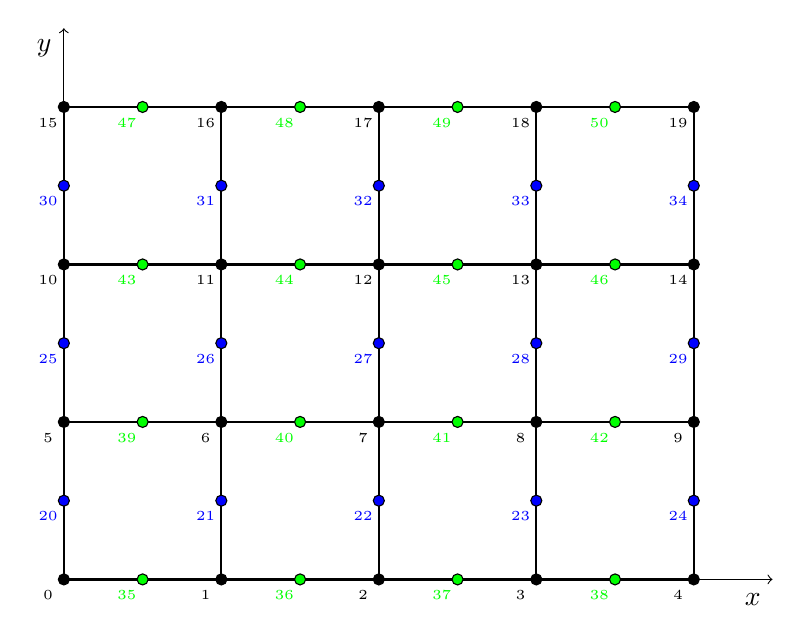
\begin{tikzpicture}
%\draw[fill=gray!23,gray!23](0,0) rectangle (10,8);
%\draw[step=0.5cm,gray,very thin] (0,0) grid (10,8); %background grid

\draw[thick] (1,1) -- (9,1) ;
\draw[thick] (1,3) -- (9,3) ;
\draw[thick] (1,5) -- (9,5) ;
\draw[thick] (1,7) -- (9,7) ;

\draw[thick] (1,1) -- (1,7) ;
\draw[thick] (3,1) -- (3,7) ;
\draw[thick] (5,1) -- (5,7) ;
\draw[thick] (7,1) -- (7,7) ;
\draw[thick] (9,1) -- (9,7) ;

\draw[black,fill=black] (1,1)   circle (2pt);
\draw[black,fill=black] (3,1)   circle (2pt);
\draw[black,fill=black] (5,1)   circle (2pt);
\draw[black,fill=black] (7,1)   circle (2pt);
\draw[black,fill=black] (9,1)   circle (2pt);

\draw[black,fill=black] (1,3)   circle (2pt);
\draw[black,fill=black] (3,3)   circle (2pt);
\draw[black,fill=black] (5,3)   circle (2pt);
\draw[black,fill=black] (7,3)   circle (2pt);
\draw[black,fill=black] (9,3)   circle (2pt);

\draw[black,fill=black] (1,5)   circle (2pt);
\draw[black,fill=black] (3,5)   circle (2pt);
\draw[black,fill=black] (5,5)   circle (2pt);
\draw[black,fill=black] (7,5)   circle (2pt);
\draw[black,fill=black] (9,5)   circle (2pt);

\draw[black,fill=black] (1,7)   circle (2pt);
\draw[black,fill=black] (3,7)   circle (2pt);
\draw[black,fill=black] (5,7)   circle (2pt);
\draw[black,fill=black] (7,7)   circle (2pt);
\draw[black,fill=black] (9,7)   circle (2pt);

\draw[black,fill=blue] (1,2) circle (2pt); 
\draw[black,fill=blue] (3,2) circle (2pt); 
\draw[black,fill=blue] (5,2) circle (2pt); 
\draw[black,fill=blue] (7,2) circle (2pt); 
\draw[black,fill=blue] (9,2) circle (2pt); 

\draw[black,fill=blue] (1,4) circle (2pt); 
\draw[black,fill=blue] (3,4) circle (2pt); 
\draw[black,fill=blue] (5,4) circle (2pt); 
\draw[black,fill=blue] (7,4) circle (2pt); 
\draw[black,fill=blue] (9,4) circle (2pt); 

\draw[black,fill=blue] (1,6) circle (2pt); 
\draw[black,fill=blue] (3,6) circle (2pt); 
\draw[black,fill=blue] (5,6) circle (2pt); 
\draw[black,fill=blue] (7,6) circle (2pt); 
\draw[black,fill=blue] (9,6) circle (2pt); 

\draw[black,fill=green] (2,1) circle (2pt); 
\draw[black,fill=green] (4,1) circle (2pt); 
\draw[black,fill=green] (6,1) circle (2pt); 
\draw[black,fill=green] (8,1) circle (2pt); 

\draw[black,fill=green] (2,3) circle (2pt); 
\draw[black,fill=green] (4,3) circle (2pt); 
\draw[black,fill=green] (6,3) circle (2pt); 
\draw[black,fill=green] (8,3) circle (2pt); 

\draw[black,fill=green] (2,5) circle (2pt); 
\draw[black,fill=green] (4,5) circle (2pt); 
\draw[black,fill=green] (6,5) circle (2pt); 
\draw[black,fill=green] (8,5) circle (2pt); 

\draw[black,fill=green] (2,7) circle (2pt); 
\draw[black,fill=green] (4,7) circle (2pt); 
\draw[black,fill=green] (6,7) circle (2pt); 
\draw[black,fill=green] (8,7) circle (2pt); 

\draw[thin,->] (9,1) -- (10,1); %x
\draw[thin,->] (1,7) -- (1,8); %y
\node[] at (9.75,0.75) {$x$};
\node[] at (0.75,7.75) {$y$};

\node[] at (0.8,0.8) {\tiny 0};
\node[] at (2.8,0.8) {\tiny 1};
\node[] at (4.8,0.8) {\tiny 2};
\node[] at (6.8,0.8) {\tiny 3};
\node[] at (8.8,0.8) {\tiny 4};
\node[] at (0.8,2.8) {\tiny 5};
\node[] at (2.8,2.8) {\tiny 6};
\node[] at (4.8,2.8) {\tiny 7};
\node[] at (6.8,2.8) {\tiny 8};
\node[] at (8.8,2.8) {\tiny 9};
\node[] at (0.8,4.8) {\tiny 10};
\node[] at (2.8,4.8) {\tiny 11};
\node[] at (4.8,4.8) {\tiny 12};
\node[] at (6.8,4.8) {\tiny 13};
\node[] at (8.8,4.8) {\tiny 14};
\node[] at (0.8,6.8) {\tiny 15};
\node[] at (2.8,6.8) {\tiny 16};
\node[] at (4.8,6.8) {\tiny 17};
\node[] at (6.8,6.8) {\tiny 18};
\node[] at (8.8,6.8) {\tiny 19};

\node[] at (0.8,1.8) {\tiny \color{blue} 20};
\node[] at (2.8,1.8) {\tiny \color{blue} 21};
\node[] at (4.8,1.8) {\tiny \color{blue} 22};
\node[] at (6.8,1.8) {\tiny \color{blue} 23};
\node[] at (8.8,1.8) {\tiny \color{blue} 24};

\node[] at (0.8,3.8) {\tiny \color{blue} 25};
\node[] at (2.8,3.8) {\tiny \color{blue} 26};
\node[] at (4.8,3.8) {\tiny \color{blue} 27};
\node[] at (6.8,3.8) {\tiny \color{blue} 28};
\node[] at (8.8,3.8) {\tiny \color{blue} 29};

\node[] at (0.8,5.8) {\tiny \color{blue} 30};
\node[] at (2.8,5.8) {\tiny \color{blue} 31};
\node[] at (4.8,5.8) {\tiny \color{blue} 32};
\node[] at (6.8,5.8) {\tiny \color{blue} 33};
\node[] at (8.8,5.8) {\tiny \color{blue} 34};

\node[] at (1.8,0.8) {\tiny \color{green} 35};
\node[] at (3.8,0.8) {\tiny \color{green} 36};
\node[] at (5.8,0.8) {\tiny \color{green} 37};
\node[] at (7.8,0.8) {\tiny \color{green} 38};

\node[] at (1.8,2.8) {\tiny \color{green} 39};
\node[] at (3.8,2.8) {\tiny \color{green} 40};
\node[] at (5.8,2.8) {\tiny \color{green} 41};
\node[] at (7.8,2.8) {\tiny \color{green} 42};

\node[] at (1.8,4.8) {\tiny \color{green} 43};
\node[] at (3.8,4.8) {\tiny \color{green} 44};
\node[] at (5.8,4.8) {\tiny \color{green} 45};
\node[] at (7.8,4.8) {\tiny \color{green} 46};

\node[] at (1.8,6.8) {\tiny \color{green} 47};
\node[] at (3.8,6.8) {\tiny \color{green} 48};
\node[] at (5.8,6.8) {\tiny \color{green} 49};
\node[] at (7.8,6.8) {\tiny \color{green} 50};

\end{tikzpicture}\\
\end{center}

For this mesh we have 

\begin{lstlisting}
nel=nelx*nely (=12) 
NP=nel (=12)
NV=nnx*nny+nnx*nely+nny*nelx (=20+16+15=51)
\end{lstlisting}

The total number of velocity dofs is 
\begin{lstlisting}
NfemV=ndofV*nnx*nny + nnx*nely + nny*nelx (=71)
\end{lstlisting}
while the total number of pressure dofs remains
\begin{lstlisting}
NfemP=NP*ndofP (=nel) 
\end{lstlisting}


There are two connectivity arrays {\tt iconu} and {\tt iconv}, both of size $mV\times nel$, where 
$mV=6$ is the number of nodes linked to an element. For each element, and depending on whether we are considering 
the polynomial approximation $u^h(x,y)$ or $v^h(x,y)$ in the element, there are the standard 4 $Q_1$ nodes and 2 additional 
dofs, so $mV=6$.
\begin{itemize}
\item content of {\tt iconu}
\begin{verbatim}
elt
0 | [ 0  1  6  5 20 21]
1 | [ 1  2  7  6 21 22]
2 | [ 2  3  8  7 22 23]
3 | [ 3  4  9  8 23 24]
4 | [ 5  6 11 10 25 26]
5 | [ 6  7 12 11 26 27]
6 | [ 7  8 13 12 27 28]
7 | [ 8  9 14 13 28 29]
8 | [10 11 16 15 30 31]
9 | [11 12 17 16 31 32]
10 | [12 13 18 17 32 33]
11 | [13 14 19 18 33 34]
\end{verbatim}
\item content of {\tt iconv}
\begin{verbatim}
elt
 0 | [ 0  1  6  5 35 39]
 1 | [ 1  2  7  6 36 40]
 2 | [ 2  3  8  7 37 41]
 3 | [ 3  4  9  8 38 42]
 4 | [ 5  6 11 10 39 43]
 5 | [ 6  7 12 11 40 44]
 6 | [ 7  8 13 12 41 45]
 7 | [ 8  9 14 13 42 46]
 8 | [10 11 16 15 43 47]
 9 | [11 12 17 16 44 48]
10 | [12 13 18 17 45 49]
11 | [13 14 19 18 46 50]
\end{verbatim}
\end{itemize}

The pressure field is normalised by imposing $\int_\Omega p dV=0 $ so that there is no nullspace.

%---------------------------------------------------------------
\subsection*{Donea \& Huerta manufactured solution benchmark}

The Donea \& huerta benchmark of Section~\ref{mms1} is implemented. It requires 
no-slip boundary conditions on all sides. This means that $u=0$ must be 
prescribed on the lateral boundaries, while $v=0$ is prescribed at the top and bottom, 
i.e. boundary conditions are imposed on the bubble nodes too.

\begin{center}
\includegraphics[width=7cm]{python_codes/fieldstone_80/results/dh/pressure}
\includegraphics[width=7cm]{python_codes/fieldstone_80/results/dh/pressure_error}\\
{\captionfont  opla}
\end{center}


Looking at the velocity and pressure error convergence, we see that the number of quadrature
points does not matter much, but surprisingly the lowest number of quad points seems to yield slightly
better results...
\begin{center}
\includegraphics[width=7.4cm]{python_codes/fieldstone_80/results/dh/errors}
\includegraphics[width=7.4cm]{python_codes/fieldstone_80/results/dh/vrms}\\
{\captionfont Left: Velocity and pressure error convergence as a function of resolution for 
different quadrature rules. Right: root mean square velocity.}
\end{center}

\begin{center}
\includegraphics[width=7cm]{python_codes/fieldstone_80/results/dh/vel}
\includegraphics[width=7cm]{python_codes/fieldstone_80/results/dh/vel_error}\\
\includegraphics[width=7cm]{python_codes/fieldstone_80/results/dh/u_dofs}
\includegraphics[width=7cm]{python_codes/fieldstone_80/results/dh/v_dofs}\\
{\captionfont Top row: velocity and velocity error. Bottom row: $u$ and 
$v$ plotted on their respective meshes.}
\end{center}

%---------------------------------------------------------------
\subsection*{The aquarium}

No-slip boundary conditions are prescribed on all sides. Density and viscosity are 1.
Gravity is $\vec{g}=-\vec{e}_y$. 

We recover a linear pressure profile as expected, that is very accurate:

\begin{center}
\includegraphics[width=7.5cm]{python_codes/fieldstone_80/results/aquarium/p}
\includegraphics[width=7.5cm]{python_codes/fieldstone_80/results/aquarium/p_error}\\
{\captionfont Left: pressure profile; Right: pressure profile error}
\end{center}

We can also record the root mean square velocity as a function of the resolution $h$
and we find that the velocity is (as expected) zero (down to machine precision):
\begin{center}
\includegraphics[width=9cm]{python_codes/fieldstone_80/results/aquarium/vrms}
\end{center}


%---------------------------------------------------------------
\subsection*{The lid driven cavity}

This is the non leaky lid driven cavity, i.e. the velocity at the top left and right corner 
is set to zero. No slip are imposed on all three other boundaries. 
The pressure field does not showcase any checkerboard mode. 

\begin{center}
\includegraphics[width=7.5cm]{python_codes/fieldstone_80/results/ldc/vel}
\includegraphics[width=7.5cm]{python_codes/fieldstone_80/results/ldc/p}
\includegraphics[width=7.5cm]{python_codes/fieldstone_80/results/ldc/u_dofs}
\includegraphics[width=7.5cm]{python_codes/fieldstone_80/results/ldc/v_dofs}\\
{\captionfont 64x64}
\end{center}

\begin{center}
\includegraphics[width=7.5cm]{python_codes/fieldstone_80/results/ldc/p_top}
\includegraphics[width=7.5cm]{python_codes/fieldstone_80/results/ldc/vrms}
\end{center}


%---------------------------------------------------------------
\subsection*{Dohrmann \& Bochev manufactured solution}

This benchmark is defined in Section~\ref{ss:mms2}.

\begin{center}
\includegraphics[width=7.5cm]{python_codes/fieldstone_80/results/db2d/vel}
\includegraphics[width=7.5cm]{python_codes/fieldstone_80/results/db2d/p}
\end{center}


\begin{center}
\includegraphics[width=7.5cm]{python_codes/fieldstone_80/results/db2d/errors}
\includegraphics[width=7.5cm]{python_codes/fieldstone_80/results/db2d/vrms}\\
{\captionfont Left: Velocity and pressure error convergence; Right: root mean square velocity
as a function of mesh size.}
\end{center}


%---------------------------------------------------------------
\subsection*{Stokes sphere}

Sphere is placed in the middle with radius 0.123, free slip boundary conditions on all sides. 
Viscosity is constant in the domain. 

\begin{center}
\includegraphics[width=5.6cm]{python_codes/fieldstone_80/results/sphere/rho_g}
\includegraphics[width=5.6cm]{python_codes/fieldstone_80/results/sphere/vel}
\includegraphics[width=5.6cm]{python_codes/fieldstone_80/results/sphere/p}\\
\includegraphics[width=5.6cm]{python_codes/fieldstone_80/results/sphere/u_dofs}
\includegraphics[width=5.6cm]{python_codes/fieldstone_80/results/sphere/v_dofs}\\
{\captionfont velocity and pressure fields for $\delta \rho=0.001$. 96x96 elements.}
\end{center}

\begin{center}
\includegraphics[width=9cm]{python_codes/fieldstone_80/results/sphere/vrms}\\
{\captionfont Root mean square velocity for $\delta \rho=0.001$, for both full density and reduced 
density models.}
\end{center}









\todo[inline]{theory and code for non-square elements}
 %%%%%%%%%%%%%%%%%%%%%%%%%%%%%%%%%%%%%%%%%%%%%%%%%

\newpage %%%%%%%%%%%%%%%%%%%%%%%%%%%%%%%%%%%%%%%%%%%%%%%%%%%%%%%%%%%%%%%%%%%%%%%%%%%%%%%%
\section*{
Stone 81: Fortin's $Q_1^+\times P_0$ in 3D 
\label{f81}}
\addcontentsline{toc}{section}{\protect\numberline{} 
Stone 81: Fortin's $Q_1^+\times P_0$ in 3D
}



\begin{center}
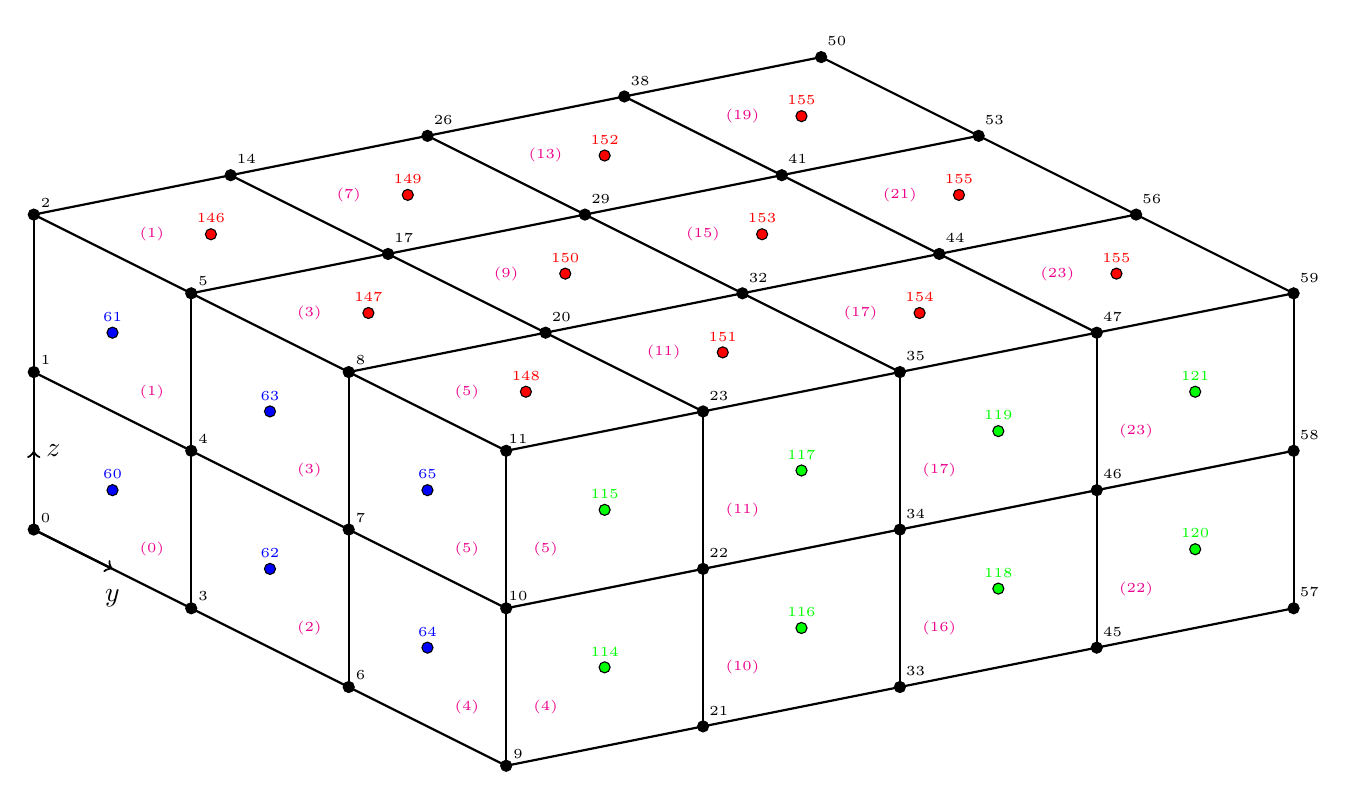
\begin{tikzpicture}
%\draw[fill=gray!23,gray!23](0,0) rectangle (16,9);
%\draw[step=0.5cm,gray,very thin] (0,0) grid (16,9); %background grid

\draw[thick] (0,3) -- (6,0) ;
\draw[thick] (0,5) -- (6,2) ;
\draw[thick] (0,7) -- (6,4) ;

\draw[thick] (2.5,7.5) -- (8.5,4.5) ;
\draw[thick] (5,8) -- (11,5) ;
\draw[thick] (7.5,8.5) -- (13.5,5.5) ;
\draw[thick] (10,9) -- (16,6) ;

\draw[thick] (0,3) -- (0,7) ;
\draw[thick] (2,2) -- (2,6) ;
\draw[thick] (4,1) -- (4,5) ;
\draw[thick] (6,0) -- (6,4) ;

\draw[thick] (0,7) -- (10,9) ;
\draw[thick] (2,6) -- (12,8) ;
\draw[thick] (4,5) -- (14,7) ;
\draw[thick] (6,4) -- (16,6) ;

\draw[thick] (6,2) -- (16,4) ;
\draw[thick] (6,0) -- (16,2) ;

\draw[thick] (8.5,0.5) -- (8.5,4.5) ;
\draw[thick] (11,1) -- (11,5) ;
\draw[thick] (13.5,1.5) -- (13.5,5.5) ;
\draw[thick] (16,2) -- (16,6) ;

\draw[black,fill=black] (0,3)   circle (2pt); \node[] at (0.15,3.15) {\tiny 0};
\draw[black,fill=black] (0,5)   circle (2pt); \node[] at (0.15,5.15) {\tiny 1};
\draw[black,fill=black] (0,7)   circle (2pt); \node[] at (0.15,7.15) {\tiny 2};

\draw[black,fill=black] (2,2)   circle (2pt); \node[] at (2.15,2.15) {\tiny 3};
\draw[black,fill=black] (2,4)   circle (2pt); \node[] at (2.15,4.15) {\tiny 4};
\draw[black,fill=black] (2,6)   circle (2pt); \node[] at (2.15,6.15) {\tiny 5};

\draw[black,fill=black] (4,1)   circle (2pt); \node[] at (4.15,1.15) {\tiny 6};
\draw[black,fill=black] (4,3)   circle (2pt); \node[] at (4.15,3.15) {\tiny 7};
\draw[black,fill=black] (4,5)   circle (2pt); \node[] at (4.15,5.15) {\tiny 8};

\draw[black,fill=black] (6,0)   circle (2pt); \node[] at (6.15,0.15) {\tiny 9};
\draw[black,fill=black] (6,2)   circle (2pt); \node[] at (6.15,2.15) {\tiny 10};
\draw[black,fill=black] (6,4)   circle (2pt); \node[] at (6.15,4.15) {\tiny 11};

\draw[black,fill=black] (8.5,0.5)   circle (2pt);  \node[] at (8.7,0.7) {\tiny 21};
\draw[black,fill=black] (8.5,2.5)   circle (2pt);  \node[] at (8.7,2.7) {\tiny 22};
\draw[black,fill=black] (8.5,4.5)   circle (2pt);  \node[] at (8.7,4.7) {\tiny 23};

\draw[black,fill=black] (11,1)   circle (2pt); \node[] at (11.2,1.2) {\tiny 33};
\draw[black,fill=black] (11,3)   circle (2pt); \node[] at (11.2,3.2) {\tiny 34};
\draw[black,fill=black] (11,5)   circle (2pt); \node[] at (11.2,5.2) {\tiny 35};

\draw[black,fill=black] (13.5,1.5)   circle (2pt); \node[] at (13.7,1.7) {\tiny 45};
\draw[black,fill=black] (13.5,3.5)   circle (2pt); \node[] at (13.7,3.7) {\tiny 46};
\draw[black,fill=black] (13.5,5.5)   circle (2pt); \node[] at (13.7,5.7) {\tiny 47};

\draw[black,fill=black] (16,2)   circle (2pt); \node[] at (16.2,2.2) {\tiny 57};
\draw[black,fill=black] (16,4)   circle (2pt); \node[] at (16.2,4.2) {\tiny 58};
\draw[black,fill=black] (16,6)   circle (2pt); \node[] at (16.2,6.2) {\tiny 59};

\draw[black,fill=black] (6.5,5.5)  circle (2pt); \node[] at (6.7,5.7) {\tiny 20};
\draw[black,fill=black] (9,6)      circle (2pt); \node[] at (9.2,6.2) {\tiny 32};
\draw[black,fill=black] (11.5,6.5) circle (2pt); \node[] at (11.7,6.7) {\tiny 44};
\draw[black,fill=black] (14,7)     circle (2pt); \node[] at (14.2,7.2) {\tiny 56};

\draw[black,fill=black] (4.5,6.5) circle (2pt); \node[] at (4.7,6.7) {\tiny 17};
\draw[black,fill=black] (7,7)     circle (2pt); \node[] at (7.2,7.2) {\tiny 29};
\draw[black,fill=black] (9.5,7.5) circle (2pt); \node[] at (9.7,7.7) {\tiny 41};
\draw[black,fill=black] (12,8)    circle (2pt); \node[] at (12.2,8.2) {\tiny 53};

\draw[black,fill=black] (2.5,7.5) circle (2pt); \node[] at (2.7,7.7) {\tiny 14};
\draw[black,fill=black] (5,8)     circle (2pt); \node[] at (5.2,8.2) {\tiny 26};
\draw[black,fill=black] (7.5,8.5) circle (2pt); \node[] at (7.7,8.7) {\tiny 38};
\draw[black,fill=black] (10,9)    circle (2pt); \node[] at (10.2,9.2) {\tiny 50};

\draw[black,fill=blue] (1,3.5) circle (2pt); \node[] at (1,3.7) {\tiny \color{blue} 60};
\draw[black,fill=blue] (1,5.5) circle (2pt); \node[] at (1,5.7) {\tiny \color{blue} 61};
\draw[black,fill=blue] (3,2.5) circle (2pt); \node[] at (3,2.7) {\tiny \color{blue} 62};
\draw[black,fill=blue] (3,4.5) circle (2pt); \node[] at (3,4.7) {\tiny \color{blue} 63};
\draw[black,fill=blue] (5,1.5) circle (2pt); \node[] at (5,1.7) {\tiny \color{blue} 64};
\draw[black,fill=blue] (5,3.5) circle (2pt); \node[] at (5,3.7) {\tiny \color{blue} 65};

\draw[black,fill=green](7.25,1.25) circle (2pt);\node[] at (7.25,1.45){\tiny\color{green}114};
\draw[black,fill=green](7.25,3.25) circle (2pt);\node[] at (7.25,3.45){\tiny\color{green}115};
\draw[black,fill=green](9.75,1.75) circle (2pt);\node[] at (9.75,1.95){\tiny\color{green}116};
\draw[black,fill=green](9.75,3.75) circle (2pt);\node[] at (9.75,3.95){\tiny\color{green}117};
\draw[black,fill=green](12.25,2.25) circle (2pt);\node[] at (12.25,2.45){\tiny\color{green}118};
\draw[black,fill=green](12.25,4.25) circle (2pt);\node[] at (12.25,4.45){\tiny\color{green}119};
\draw[black,fill=green](14.75,2.75) circle (2pt);\node[] at (14.75,2.95){\tiny\color{green}120};
\draw[black,fill=green](14.75,4.75) circle (2pt);\node[] at (14.75,4.95){\tiny\color{green}121};

\draw[black,fill=red] (2.25,6.75) circle (2pt); \node[] at (2.25,6.95) {\tiny \color{red} 146};
\draw[black,fill=red] (4.25,5.75) circle (2pt); \node[] at (4.25,5.95) {\tiny \color{red} 147};
\draw[black,fill=red] (6.25,4.75) circle (2pt); \node[] at (6.25,4.95) {\tiny \color{red} 148};

\draw[black,fill=red] (4.75,7.25) circle (2pt); \node[] at (4.75,7.45) {\tiny \color{red} 149};
\draw[black,fill=red] (6.75,6.25) circle (2pt); \node[] at (6.75,6.45) {\tiny \color{red} 150};
\draw[black,fill=red] (8.75,5.25) circle (2pt); \node[] at (8.75,5.45) {\tiny \color{red} 151};

\draw[black,fill=red] (7.25,7.75) circle (2pt); \node[] at (7.25,7.95) {\tiny \color{red} 152};
\draw[black,fill=red] (9.25,6.75) circle (2pt); \node[] at (9.25,6.95) {\tiny \color{red} 153};
\draw[black,fill=red] (11.25,5.75) circle (2pt); \node[] at (11.25,5.95) {\tiny \color{red} 154};

\draw[black,fill=red] (9.75,8.25) circle (2pt); \node[] at (9.75,8.45) {\tiny \color{red} 155};
\draw[black,fill=red] (11.75,7.25) circle (2pt); \node[] at (11.75,7.45) {\tiny \color{red} 155};
\draw[black,fill=red] (13.75,6.25) circle (2pt); \node[] at (13.75,6.45) {\tiny \color{red} 155};

\node[] at (1.5,2.75) {\tiny \color{magenta} (0)};
\node[] at (1.5,4.75) {\tiny \color{magenta} (1)};
\node[] at (3.5,1.75) {\tiny \color{magenta} (2)};
\node[] at (3.5,3.75) {\tiny \color{magenta} (3)};
\node[] at (5.5,0.75) {\tiny \color{magenta} (4)};
\node[] at (5.5,2.75) {\tiny \color{magenta} (5)};

\node[] at (6.5,0.75) {\tiny \color{magenta} (4)};
\node[] at (6.5,2.75) {\tiny \color{magenta} (5)};
\node[] at (9,1.25) {\tiny \color{magenta} (10)};
\node[] at (9,3.25) {\tiny \color{magenta} (11)};
\node[] at (11.5,1.75) {\tiny \color{magenta} (16)};
\node[] at (11.5,3.75) {\tiny \color{magenta} (17)};
\node[] at (14,2.25) {\tiny \color{magenta} (22)};
\node[] at (14,4.25) {\tiny \color{magenta} (23)};

\node[] at (5.5,4.75) {\tiny \color{magenta} (5)};
\node[] at (8,5.25) {\tiny \color{magenta} (11)};
\node[] at (10.5,5.75) {\tiny \color{magenta} (17)};
\node[] at (13,6.25) {\tiny \color{magenta} (23)};

\node[] at (3.5,5.75) {\tiny \color{magenta} (3)};
\node[] at (6,6.25) {\tiny \color{magenta} (9)};
\node[] at (8.5,6.75) {\tiny \color{magenta} (15)};
\node[] at (11,7.25) {\tiny \color{magenta} (21)};

\node[] at (1.5,6.75) {\tiny \color{magenta} (1)};
\node[] at (4,7.25) {\tiny \color{magenta} (7)};
\node[] at (6.5,7.75) {\tiny \color{magenta} (13)};
\node[] at (9,8.25) {\tiny \color{magenta} (19)};

\draw[thick,->] (0,3) -- (0,4); %x
\draw[thick,->] (0,3) -- (1,2.5); %y
\node[] at (1,2.125) {$y$};
\node[] at (0.25,4) {$z$};

\end{tikzpicture}\\
\end{center}

Each element has 
\begin{itemize}
\item 8+2 u dofs
\item 8+2 v dofs
\item 8+2 w dofs
\end{itemize}

Setting nelx=4, nely=3 and nelz=2, we can print the three connectivity arrays:

\begin{itemize}
\item iconu:

\begin{verbatim}
0 [ 0 12 15  3  1 13 16  4 60 66]
1 [ 1 13 16  4  2 14 17  5 61 67]
2 [ 3 15 18  6  4 16 19  7 62 68]
3 [ 4 16 19  7  5 17 20  8 63 69]
4 [ 6 18 21  9  7 19 22 10 64 70]
5 [ 7 19 22 10  8 20 23 11 65 71]
6 [12 24 27 15 13 25 28 16 66 72]
7 [13 25 28 16 14 26 29 17 67 73]
8 [15 27 30 18 16 28 31 19 68 74]
9 [16 28 31 19 17 29 32 20 69 75]
10 [18 30 33 21 19 31 34 22 70 76]
11 [19 31 34 22 20 32 35 23 71 77]
12 [24 36 39 27 25 37 40 28 72 78]
13 [25 37 40 28 26 38 41 29 73 79]
14 [27 39 42 30 28 40 43 31 74 80]
15 [28 40 43 31 29 41 44 32 75 81]
16 [30 42 45 33 31 43 46 34 76 82]
17 [31 43 46 34 32 44 47 35 77 83]
18 [36 48 51 39 37 49 52 40 78 84]
19 [37 49 52 40 38 50 53 41 79 85]
20 [39 51 54 42 40 52 55 43 80 86]
21 [40 52 55 43 41 53 56 44 81 87]
22 [42 54 57 45 43 55 58 46 82 88]
23 [43 55 58 46 44 56 59 47 83 89]
\end{verbatim}

\item iconv:
\begin{verbatim}
0 [ 0 12 15  3  1 13 16  4 90 98]
1 [ 1 13 16  4  2 14 17  5 91 99]
2 [  3  15  18   6   4  16  19   7  98 106]
3 [  4  16  19   7   5  17  20   8  99 107]
4 [  6  18  21   9   7  19  22  10 106 114]
5 [  7  19  22  10   8  20  23  11 107 115]
6 [ 12  24  27  15  13  25  28  16  92 100]
7 [ 13  25  28  16  14  26  29  17  93 101]
8 [ 15  27  30  18  16  28  31  19 100 108]
9 [ 16  28  31  19  17  29  32  20 101 109]
10 [ 18  30  33  21  19  31  34  22 108 116]
11 [ 19  31  34  22  20  32  35  23 109 117]
12 [ 24  36  39  27  25  37  40  28  94 102]
13 [ 25  37  40  28  26  38  41  29  95 103]
14 [ 27  39  42  30  28  40  43  31 102 110]
15 [ 28  40  43  31  29  41  44  32 103 111]
16 [ 30  42  45  33  31  43  46  34 110 118]
17 [ 31  43  46  34  32  44  47  35 111 119]
18 [ 36  48  51  39  37  49  52  40  96 104]
19 [ 37  49  52  40  38  50  53  41  97 105]
20 [ 39  51  54  42  40  52  55  43 104 112]
21 [ 40  52  55  43  41  53  56  44 105 113]
22 [ 42  54  57  45  43  55  58  46 112 120]
23 [ 43  55  58  46  44  56  59  47 113 121]
\end{verbatim}

\item iconw:
\begin{verbatim}
0 [  0  12  15   3   1  13  16   4 122 134]
1 [  1  13  16   4   2  14  17   5 134 146]
2 [  3  15  18   6   4  16  19   7 123 135]
3 [  4  16  19   7   5  17  20   8 135 147]
4 [  6  18  21   9   7  19  22  10 124 136]
5 [  7  19  22  10   8  20  23  11 136 148]
6 [ 12  24  27  15  13  25  28  16 125 137]
7 [ 13  25  28  16  14  26  29  17 137 149]
8 [ 15  27  30  18  16  28  31  19 126 138]
9 [ 16  28  31  19  17  29  32  20 138 150]
10 [ 18  30  33  21  19  31  34  22 127 139]
11 [ 19  31  34  22  20  32  35  23 139 151]
12 [ 24  36  39  27  25  37  40  28 128 140]
13 [ 25  37  40  28  26  38  41  29 140 152]
14 [ 27  39  42  30  28  40  43  31 129 141]
15 [ 28  40  43  31  29  41  44  32 141 153]
16 [ 30  42  45  33  31  43  46  34 130 142]
17 [ 31  43  46  34  32  44  47  35 142 154]
18 [ 36  48  51  39  37  49  52  40 131 143]
19 [ 37  49  52  40  38  50  53  41 143 155]
20 [ 39  51  54  42  40  52  55  43 132 144]
21 [ 40  52  55  43  41  53  56  44 144 156]
22 [ 42  54  57  45  43  55  58  46 133 145]
23 [ 43  55  58  46  44  56  59  47 145 157]
\end{verbatim}

\end{itemize}




%----------------------------------------------------
\subsection*{Manufactured solution}

This benchmark is presented in Section~\ref{mms3}. It was run with 3 different quadrature levels, $nq=2^3,3^3,4^3$. 
Unfortunately a resolution 20x20x20 is the maximum which can be run. 

\begin{center}
\includegraphics[width=10cm]{python_codes/fieldstone_81/results/conv.pdf}
\end{center}





 %%%%%%%%%%%%%%%%%%%%%%%%%%%%%%%%%%%%%%%%%%%%%%%%%

%\newpage %%%%%%%%%%%%%%%%%%%%%%%%%%%%%%%%%%%%%%%%%%%%%%%%%%%%%%%%%%%%%%%%%%%%%%%%%%%%%%%%
%\section*{
%Stone 82: The 3D MINI element with 2 bubble functions 
%\label{f82}}
%\addcontentsline{toc}{section}{\protect\numberline{} 
%Stone 82: The 3D MINI element with 2 bubble functions 
%}
%
The basis functions for this element is presented in Section~\ref{ss:Q1Q1bb_3D}.
This element is presented in Karabelas \etal (2020) \cite{kahp20}. 

There are two bubble functions/nodes per element so we then have 
\begin{lstlisting}
NV=nnx*nny*nnz+2*nel 
NP=nnx*nny*nnz
\end{lstlisting}
For a 8x8x8=512 element grid, there are $9^3=729$ nodes, and 1024 bubble nodes.
We then have $3\cdot 729=2157$ $Q_1$ velocity dofs and 3072 velocity dofs attached 
to the bubbles.
Since the bubble nodes are stored last the structure of the matrix is as follows:
\begin{center}
\includegraphics[width=6cm]{python_codes/fieldstone_82/results/matrix_8x8x8_bef_bc}
\includegraphics[width=6cm]{python_codes/fieldstone_82/results/matrix_8x8x8_aft_bc}\\
{\captionfont Sparsity pattern of the matrix for a 8x8x8 grid.
NV= 1753, NP=729.\\ Left:
before boundary conditions are applied. 
Right: after boundary conditions are applied.} 
\end{center}


%......................................
\subsubsection*{Manufactured solution (bench=1)}

This benchmark begins by postulating a polynomial solution 
to the 3D Stokes equation (see Dohrmann \& Bochev (2004) \cite{dobo04}):
\begin{equation}
\vec{\upnu}(x,y,z)
=
\left(
\begin{array}{c}
x+x^2+xy+x^3y \\
y + xy + y^2 + x^2 y^2\\
-2z - 3xz - 3yz - 5x^2 yz
\end{array}
\right)
\label{eqbur2}
\end{equation}
and
\begin{equation}
p(x,y,z) = xyz + x^3 y^3z - 5/32
\end{equation}
The corresponding right-hand side is computed in Section~\ref{mms3}.
The domain is a unit cube and velocity boundary conditions
simply use Eq. (\ref{eqbur2}).
Note that the pressure fulfills $\int_\Omega p(x,y,z) dV = 0.$

\begin{center}
\includegraphics[width=8cm]{python_codes/fieldstone_82/results/bench1/vrms.pdf}
\includegraphics[width=8cm]{python_codes/fieldstone_82/results/bench1/conv.pdf}\\
{\captionfont Results obtained for three levels of quadrature, with $\beta=0$ (i.e.
viscosity is constant and equal to 1).}
\end{center}

Somewhat surprisingly, the pressure convergence is not exactly quadratic but seems to be
around 1.8. Also, the $2\times 2\times 2$ 
quadrature yields better results than the $3\times 3\times 3$ or $4\times 4 \times 4$.

%......................................
\subsubsection*{Horizontal shear (bench=2)}

This is a simple kinematical test: gravity is set to zero, no boundary 
conditions on the sides and $\vec\upnu=(-1,0,0)$ prescribed on the top, and 
$\vec\upnu=(+1,0,0)$ prescribed on the bottom.

\begin{center}
\includegraphics[width=6cm]{python_codes/fieldstone_82/results/bench2/vel}
\includegraphics[width=6cm]{python_codes/fieldstone_82/results/bench2/press}\\
{\captionfont 20x20x20 mesh.} 
\end{center}

%......................................
\subsubsection*{Stokes sphere (bench=3)}

This is the benchmark of Section~\ref{ss:stokes_sphere3D}.
A sphere of radius 0.123456789 is placed in the middle of the domain. 
It has a density excess $\delta\rho=0.01$
with respect to the surrounding fluid which has a density $\rho_{fluid}=1$. 
The sphere viscosity is 1000 why the fluid viscosity is 1.
Boundary conditions are no slip on all sides. Gravity is $\vec{g}=-\vec{e}_z$.

\begin{center}
\includegraphics[width=5cm]{python_codes/fieldstone_82/results/bench3/grid.png}
\includegraphics[width=5cm]{python_codes/fieldstone_82/results/bench3/vel.png}
\includegraphics[width=5cm]{python_codes/fieldstone_82/results/bench3/press.png}\\
\includegraphics[width=5cm]{python_codes/fieldstone_82/results/bench3/u.png}
\includegraphics[width=5cm]{python_codes/fieldstone_82/results/bench3/v.png}
\includegraphics[width=5cm]{python_codes/fieldstone_82/results/bench3/w.png}\\
{\captionfont Resolution $20\times 20\times 20$. Quadrature $2\times 2 \times 2$.} 
\end{center}

All velocity and pressure statistics are presented in Section~\ref{ss:stokes_sphere3D}.

\begin{center}
\includegraphics[width=8cm]{python_codes/fieldstone_82/results/bench3/build.pdf}
\includegraphics[width=8cm]{python_codes/fieldstone_82/results/bench3/solve.pdf}\\
{\captionfont Matrix build and solve time as a function of $h$.}
\end{center}

%......................................
\subsubsection*{Sinking cube (bench=4)}

This is the same experiment as the Stokes sphere with the exception of the geometry of the sinker which 
is 0.25x0.25x0.25 in size so that its edges align with boundary edges for 8x8x8, 16x16x16 and 24x24x24 meshes.
Reduced density is used in order to remove the lithostatic pressure signal.
 
\begin{center}
\includegraphics[width=8cm]{python_codes/fieldstone_82/results/bench4/rho}
\includegraphics[width=8cm]{python_codes/fieldstone_82/results/bench4/vel}\\
{\captionfont resolution 24x24x24 elements.}
\end{center}

The velocity and pressures are interpolated on 100 points on the four diagonals of the cube
as a way to verify the symmetry of the solution (the bubbles rely on the basis 
functions of nodes 0 and 6 afterall!). $2^3$ quadrature points per element are used. 

\begin{center}
\includegraphics[width=5.5cm]{python_codes/fieldstone_82/results/bench4/u_08}
\includegraphics[width=5.5cm]{python_codes/fieldstone_82/results/bench4/u_16}
\includegraphics[width=5.5cm]{python_codes/fieldstone_82/results/bench4/u_24}\\
\includegraphics[width=5.5cm]{python_codes/fieldstone_82/results/bench4/v_08}
\includegraphics[width=5.5cm]{python_codes/fieldstone_82/results/bench4/v_16}
\includegraphics[width=5.5cm]{python_codes/fieldstone_82/results/bench4/v_24}\\
\includegraphics[width=5.5cm]{python_codes/fieldstone_82/results/bench4/w_08}
\includegraphics[width=5.5cm]{python_codes/fieldstone_82/results/bench4/w_16}
\includegraphics[width=5.5cm]{python_codes/fieldstone_82/results/bench4/w_24}\\
\includegraphics[width=5.5cm]{python_codes/fieldstone_82/results/bench4/p_08}
\includegraphics[width=5.5cm]{python_codes/fieldstone_82/results/bench4/p_16}
\includegraphics[width=5.5cm]{python_codes/fieldstone_82/results/bench4/p_24}\\
{\captionfont Left to right: increasing resolution}
\end{center}

We can also plot the velocity and pressure fields on a vertical line passing 
through the middle of the block:
\begin{center}
\includegraphics[width=5.5cm]{python_codes/fieldstone_82/results/bench4/vert_u}
\includegraphics[width=5.5cm]{python_codes/fieldstone_82/results/bench4/vert_v}
\includegraphics[width=5.5cm]{python_codes/fieldstone_82/results/bench4/vert_w}
\includegraphics[width=5.5cm]{python_codes/fieldstone_82/results/bench4/vert_p}
\end{center}
We see that unfortunately the resolution 24x24x24 is most certainly not high 
enough to speak of capturing the true solution of the problem...




%......................................
\subsubsection*{Manufactured solution (bench=5)}

We here consider the manufactured solution which is introduced in Section~\ref{ss:mms3Dgen}.
The velocity and pressure fields are:
\begin{eqnarray}
u(x,y,z) &=& x(1-x)(1-2y)(1-2z)\\
v(x,y,z) &=& (1-2x) y(1-y) (1-2z) \\
w(x,y,z) &=& -2(1-2x)(1-2y)z(1-z) \\
p(x,y,z) &=& (2x-1)(2y-1)(2z-1)
\end{eqnarray}
This flow field has the built-in property that there is no flux through the 
boundaries.

\begin{center}
\includegraphics[width=8cm]{python_codes/fieldstone_82/results/bench5/vrms.pdf}
\includegraphics[width=8cm]{python_codes/fieldstone_82/results/bench5/conv.pdf}\\
{\captionfont Results obtained for three levels of quadrature.}
\end{center}


\begin{center}
\includegraphics[width=8cm]{python_codes/fieldstone_82/results/bench5/p_stats.pdf}
\includegraphics[width=8cm]{python_codes/fieldstone_82/results/bench5/times.pdf}
\end{center}







 %%%%%%%%%%%%%%%%%%%%%%%%%%%%%%%%%%%%%%%%%%%%%%%%%

\newpage %%%%%%%%%%%%%%%%%%%%%%%%%%%%%%%%%%%%%%%%%%%%%%%%%%%%%%%%%%%%%%%%%%%%%%%%%%%%%%%%
\section*{
Stone 83: Thermal structure of oceanic and continental lithosphere 
\label{f83}}
\addcontentsline{toc}{section}{\protect\numberline{} 
Stone 83: Thermal structure of oceanic and continental lithosphere 
}
\lstinputlisting[language=bash,basicstyle=\small]{python_codes/fieldstone_83/keywords}

\begin{center}
Code at \url{https://github.com/cedrict/fieldstone/tree/master/python_codes/fieldstone_83}
\end{center}

\par\noindent\rule{\textwidth}{0.4pt}

{\sl This stone was developed in collaboration with Iris van Zelst}. \index{contributors}{I. van Zelst}

\par\noindent\rule{\textwidth}{0.4pt}
%%%%%%%%%%%%%%%%%%%%%%%%%%%%%%%%%%%%%%%%%%%%%%%%%%%%%%%%%%%%%%%%%%%%%%%%%%%%%%%%%%%%%%%%%%%%%%


To accurately study the thermal structure of the oceanic lithosphere, it is important to take 
into account the temperature dependence of thermal parameters such as the thermal conductivity $k$, 
heat capacity $C_p$, and the density $\rho$. Classic (analytical) models, such as the half-space 
cooling model and the plate model, typically ignore this complexity and assume constant parameters. 
Here, we model the thermal structure of oceanic lithosphere with temperature-dependent 
thermal conductivity, heat capacity, and density according to McKenzie et al. (2005) \cite{mcjp05} 
and Richards et al. (2018) \cite{rihc18}. We use a 2D approach, although there is no lateral variation, 
which essentially makes this a 1D model of cooling oceanic lithosphere with time. 
We implement various options for the temperature-dependence of the parameters (including the constant case) 
based on experimental findings and different rock compositions 
(i.e., Parsons and Slater (1977) \cite{pasc77}, 
Berman 1988, Berman and Aranovich 1996, Hofmeister 1999, Xu et al., 2004). 
We then compare our results to those of Richards et al. (2018).

We start from Eq.(1) of McKenzie et al (2005) \cite{mcjp05}:
\[
\frac{\partial}{\partial t}(\rho(T) C_p(T) T) = \vec\nabla \cdot (k(T) \vec\nabla T)
\]
Using a simple Euler scheme we have
\[
\frac{(\rho(T) C_p(T) T)^{n} - (\rho(T) C_p(T) T)^{n-1} }{\delta t} 
 = \vec\nabla \cdot (k(T^n) \vec\nabla T^n)
\]
or, 
\[
\rho(T^n) C_p(T^n) T^{n} - \delta t \vec\nabla \cdot (k(T^n) \vec\nabla T^n)
= \rho(T^{n-1}) C_p(T^{n-1}) T^{n-1} 
\]
We left multiply by a shape function $N_i$ and integrate over the whole domain $\Omega$:
\[
\int_\Omega N_i \rho(T^n) C_p(T^n) T^{n} dV-
\delta t \int_\Omega N_i \vec\nabla \cdot (k(T^n) \vec\nabla T^n) dV
= 
\int_\Omega N_i\rho(T^{n-1}) C_p(T^{n-1}) T^{n-1} dV
\]
Inside an element we have 
\[
T^h = \vec{N} \cdot \vec{T}
\]
and taking $i=1,m$ yields (see Section~\ref{ss:hte_fem})
\[
{\bm M}^n \cdot \vec{T}^n + {\bm K}^n \cdot \vec{T} ^n = \vec{f}^{n-1}
\]
with
\begin{eqnarray}
{\bm M}^n &=& \int_V \rho(T^n) C_p(T^n) \vec{N}^T \vec{N} dV  \nn\\
{\bm K}^n &=& \int_V {\bm B}^T k(T^n) {\bm B} dV \nn\\
\vec{f}^{n-1} &=& \int_V \vec{N}^T \rho(T^{n-1}) C_p(T^{n-1}) dV \nn
\end{eqnarray}
The second term has been integrated by parts (and the surface term disregarded:
Dirichlet boundary conditions top and bottom, and zero heat flux on the sides).


The density is given by Eq.(9) of \cite{mcjp05}:
\begin{equation}
\rho(T)=\rho_0 \exp -\left[\alpha_0 (T-273) + \frac{\alpha_1}{2} (T^2-273^2) \right]
\label{eq:f83_1}
\end{equation}
with $\rho_0=3330\si{\kg\per\cubic\meter}$.

The heat capacity is given by Eq.(10) of \cite{mcjp05}:
\begin{equation}
C_p(T) = k_0 + k_1 T^{-1/2} + k_3 T^{-3}
\label{eq:f83_2}
\end{equation}
with $k_0=233.18$, $k_1=-1801.6$ and $k_3=-26.794\cdot 10^{7}$ for fosterite and 
$k_0=252$, $k_1=-2013.7$ and $k_3=-6.219\cdot10^{7}$ for fayalite. We assumed that the
molar fraction of fayalite in the mantle is 11\%. 

The heat conductivity is given by Eq.(4) of \cite{mcjp05}:
\begin{equation}
k(T)=\frac{b}{a+cT} + \sum_{m=0}^3 d_m (T+273)^m
\label{eq:f83_3}
\end{equation}
with $b=5.3$, $c=0.0015$, $d_0=1.753\cdot10^{-2}$, $d_1=-1.0365\cdot10^{-4}$, $d_2=2.2451\cdot10^{-7}$ and 
$d_3=-3.4071\cdot10^{-11}$


Because the coefficients $\rho(T)$, $C_p(T)$ and $k(T)$ depend on the temperature, which is the unknown 
of the PDE, this PDE is highly nonlinear and a dedicated algorithm {\it should} then be designed to handle the 
nonlinearity. For now the code disregards those considerations and its structure is identical to the linear equation case.

Following Richards et al, we run the model for 170Myr. Boundary conditions are $T=0\si{\celsius}$ 
at the top and $T=1350\si{\celsius}$ at the bottom. The functions for $k(T)$, $C_p(T)$ and $\rho(T)$
are in a separate file {\sl temperature\_dependent\_variables.py}.

%.....................................
\subsection*{Constant parameters}

In this case we set $k=3.138$, $C_p=1171.52$ and $\rho=3330$.


\begin{center}
\includegraphics[width=12cm]{python_codes/fieldstone_83/images/rihc18a}\\
{\captionfont Taken from Richards et al (2018) \cite{rihc18}.
Thermal structure of oceanic lithosphere. 
(a) Simple analytical plate model using the published values reported by Parsons and Sclater (1977) \cite{pasc77}; 
numbered contours = isothermal surfaces plotted in \si{\celsius}; 
green and white circles with error bars = oceanic intraplate and outer rise earthquakes 
from Craig et al. (2014) where small/medium/large circles 
= $M_b < 5.5$, $5.5-6.5$, and $> 6.5$; 
vertical black bars = depth to lithosphere-asthenosphere boundary in the Pacific Ocean
based upon peak variations in azimuthal anisotropy (Burgos et al., 2014); 
dashed box = envelope of depths to lithosphere-asthenosphere boundary for plate 
ages $>100$ Ma (Steinberger \& Becker (2018) \cite{stbe18}); 
horizontal black dashed line = base of plate model. 
} 
\end{center}

\begin{center}
\includegraphics[width=7cm]{python_codes/fieldstone_83/results_model1/T.png}
\includegraphics[width=7cm]{python_codes/fieldstone_83/results_model1/comparison.png}\\
{\captionfont Isocontours every 100$\si{\celsius}$ between 0 and 1300.}
\end{center}

\begin{center}
\includegraphics[width=10cm]{python_codes/fieldstone_83/results_model1/Tprofiles}\\
{\captionfont Temperature profile evolution.} 
\end{center}



%.....................................
\subsection*{T-dependent parameters a la McKenzie et al (2015)}

\begin{center}
\includegraphics[width=12cm]{python_codes/fieldstone_83/images/rihc18b}\\
{\captionfont Same for the purely temperature-dependent plate model using parameter values from
McKenzie et al. (2005) \cite{mcjp05}.}
\end{center}

\begin{center}
\includegraphics[width=5cm]{python_codes/fieldstone_83/results_model2/rho.pdf}
\includegraphics[width=5cm]{python_codes/fieldstone_83/results_model2/hcapa.pdf}
\includegraphics[width=5cm]{python_codes/fieldstone_83/results_model2/hcond.pdf}\\
{\captionfont Density, heat capacity and heat conductivity as obtained from Eqs.~\eqref{eq:f83_1}, \eqref{eq:f83_2}, and \eqref{eq:f83_3}.}
\end{center}


\begin{center}
\includegraphics[width=7cm]{python_codes/fieldstone_83/results_model2/T}
\includegraphics[width=7cm]{python_codes/fieldstone_83/results_model2/k}\\
\includegraphics[width=7cm]{python_codes/fieldstone_83/results_model2/Cp}
\includegraphics[width=7cm]{python_codes/fieldstone_83/results_model2/rho.png}\\
{\captionfont RERUN}
\end{center}

\begin{center}
\includegraphics[width=10cm]{python_codes/fieldstone_83/results_model2/Tprofiles}\\
{\captionfont Temperature profile evolution.}
\end{center}


 %%%%%%%%%%%%%%%%%%%%%%%%%%%%%%%%%%%%%%%%%%%%%%%%%

\newpage %%%%%%%%%%%%%%%%%%%%%%%%%%%%%%%%%%%%%%%%%%%%%%%%%%%%%%%%%%%%%%%%%%%%%%%%%%%%%%%%
\section*{
Stone 84: computing gravity above objects 
\label{f84}}
\addcontentsline{toc}{section}{\protect\numberline{} 
Stone 84: computing gravity above objects 
}
\lstinputlisting[language=bash,basicstyle=\small]{python_codes/fieldstone_84/keywords}

\begin{center}
Code at \url{https://github.com/cedrict/fieldstone/tree/master/python_codes/fieldstone_84}
\end{center}

\par\noindent\rule{\textwidth}{0.4pt}

{\sl This stone was developed in collaboration wth Sverre Hassing}. \index{contributors}{S. Hassing}

\par\noindent\rule{\textwidth}{0.4pt}
%%%%%%%%%%%%%%%%%%%%%%%%%%%%%%%%%%%%%%%%%%%%%%%%%%%%%%%%%%%%%%%%%%%%%%%%%%%%%%%%%%%%%%%%%%%%%%

This stone deals with the forward calculations of gravity fields (potential, vector and tensor).
It implements to different ways: 
\begin{itemize}
\item the point mass approach: each cell of size $(h_x,h_y,h_z)$ and of constant density $\rho$
is contracted to a single point in its middle of equivalent mass $m=\rho h_xh_yh_z$.
\item the prism approach, as explained in Appendix~\ref{app:prisms}.
\item the Gauss quadrature approach using $n_q^3$ points per cell.
\end{itemize}

Three types of gravity measurements are implemented:
\begin{itemize}
\item on a plane, defined by z=z\_{plane}, of size $Lx \times Ly$, counting nnx\_plane X nny\_plane points
\item on a line, starting at point (x\_begin,y\_begin,z\_begin) and ending at point (x\_end,y\_end,z\_end)
\item at a single point, atcoordinates xpt,ypt,zpt from the center of the object
\item on a 3D spiral starting at the north pole and going to the south pole, parameterised only 
by the total number of points and the distance to the center/radius of all spiral points.
This is called the Fibonacci spiral, or lattice on a sphere. The code is borrowed from the 
one in the gravity post-processor of ASPECT.
\end{itemize}

We will try to answer those questions:
Is it worth using prisms instead of mass points ?  
If so, how much more accurate are the former than the latter?
How much more expensive in terms of cpu time are prism-based calculations ?
What about the Gauss quadrature approach ? 

The domain is a cuboid of size $L_x\times L_y \times L_z$ cut into $nel_x \times nel_y \times nel_z=nel$ cells.
Note that in all what follows a cell has a constant density. 

The function {\tt grav\_calc} computes $u$, $\vec{g}$ and ${\bm T}$ using one of the three methods hilighted above. 

Note that the \aspect postprocessor relies on the Gauss-Legendre quadrature, see also von Frese \etal \cite{vohb81}.

\newpage
%-------------------------------
\subsection*{Buried sphere}

The domain is a cube of $L=1\si{\km}$ size. All elements inside a sphere of radius $R=L/2$ are assigned
$\rho_s=100\si{\kg\per\cubic\metre}$.
The mass of the sphere is 
\[
M_s = \frac{4}{3}\pi R^3 \rho \simeq 5.23598775598 \cdot 10^{10} \si{kg}
\]
So that outside of the sphere the gravity field and potential are trivial to compute:
\[
|\vec{g}(r)|={\cal G}\frac{M_s}{r^2}
\qquad
\qquad
U(r)={\cal G}\frac{M_s}{r}
\]
Gravity terms are computed on a line starting at $\vec{r}=(0,0,0)$ and ending at $\vec{r}=(1.11,2.22,5.55)\si{km}$ (this is to avoid any cancelling due to symmetry).
The analytical expressions for the gravity and gravity potential are 
\begin{eqnarray}
|\vec{g}(r)|=g(r) 
&=& {\cal G} \rho \frac{4}{3}\pi r \qquad \text{inside} \nn\\
&=& {\cal G} \rho \frac{4}{3}\pi \frac{R^3}{r^2}  \qquad \text{outside} \nn\\
U(r) 
&=& - 2 \pi {\cal G} \rho (R^2-r^2/3) \qquad \text{inside} \nn\\
&=& - {\cal G} \rho \frac{4}{3}\pi \frac{R^3}{r}  \qquad \text{outside} \nn
\end{eqnarray}

\begin{center}
\includegraphics[width=8cm]{python_codes/fieldstone_84/sphere/setup}
\end{center}


\begin{center}
\includegraphics[width=8cm]{python_codes/fieldstone_84/sphere/gravnorm}
\includegraphics[width=8cm]{python_codes/fieldstone_84/sphere/gravpot}\\
\includegraphics[width=8cm]{python_codes/fieldstone_84/sphere/gravnorm_error}
\includegraphics[width=8cm]{python_codes/fieldstone_84/sphere/gravpot_error}\\
{\captionfont  The grey area indicates the sphere. Mesh resolution?}
\end{center}

The gravity was also measured at location $(123,234,345)\si{\metre}$ counted from the center of the sphere
for increasing resolutions. 

\begin{center}
\includegraphics[width=8cm]{python_codes/fieldstone_84/sphere/single_point_g.pdf}
\includegraphics[width=8cm]{python_codes/fieldstone_84/sphere/single_point_U.pdf}\\
\includegraphics[width=8cm]{python_codes/fieldstone_84/sphere/single_point_g_error.pdf}
\includegraphics[width=8cm]{python_codes/fieldstone_84/sphere/single_point_U_error.pdf}
\end{center}


\newpage
%-------------------------------
\subsection*{Buried cube}

The domain is a cube of $L=1\si{\km}$ size. All elements inside a cube of size $d=L/8$ are assigned
$\rho_s=100\si{\kg\per\cubic\metre}$.
The mass of the cube is then
\[
M_c = \rho d^3 = 1.95312500\cdot 10^8 \si{\kg}
\]
Far away from the cube $g(r) \rightarrow {\cal G}M_c \rho/r^2$ and $U(r) \rightarrow -{\cal G} M_c/r$.

\begin{center}
\includegraphics[width=6cm]{python_codes/fieldstone_84/cube/setup}
\end{center}


\begin{center}
\includegraphics[width=7cm]{python_codes/fieldstone_84/cube/gravnorm}
\includegraphics[width=7cm]{python_codes/fieldstone_84/cube/gravpot}\\
\includegraphics[width=5cm]{python_codes/fieldstone_84/cube/tensor_xx}
\includegraphics[width=5cm]{python_codes/fieldstone_84/cube/tensor_yy}
\includegraphics[width=5cm]{python_codes/fieldstone_84/cube/tensor_zz}\\
\includegraphics[width=5cm]{python_codes/fieldstone_84/cube/tensor_xy}
\includegraphics[width=5cm]{python_codes/fieldstone_84/cube/tensor_xz}
\includegraphics[width=5cm]{python_codes/fieldstone_84/cube/tensor_yz}\\
{\captionfont  The grey area indicates the sphere. resolution  32x32x32}
\end{center}



\begin{center}
\includegraphics[width=5cm]{python_codes/fieldstone_84/cube/g}
\includegraphics[width=5cm]{python_codes/fieldstone_84/cube/U}
\includegraphics[width=5cm]{python_codes/fieldstone_84/cube/horgrad}
\end{center}

\begin{center}
\includegraphics[width=5cm]{python_codes/fieldstone_84/cube/Txx}
\includegraphics[width=5cm]{python_codes/fieldstone_84/cube/Tyy}
\includegraphics[width=5cm]{python_codes/fieldstone_84/cube/Tzz}\\
\includegraphics[width=5cm]{python_codes/fieldstone_84/cube/Txy}
\includegraphics[width=5cm]{python_codes/fieldstone_84/cube/Txz}
\includegraphics[width=5cm]{python_codes/fieldstone_84/cube/Tyz}\\
{\captionfont  xxx}
\end{center}

The gravity was also measured at location $(12,23,34)\si{\metre}$ counted from the center of the cube
for increasing resolutions. 

\begin{center}
\includegraphics[width=8cm]{python_codes/fieldstone_84/cube/single_point_g.pdf}
\includegraphics[width=8cm]{python_codes/fieldstone_84/cube/single_point_U.pdf}\\
\includegraphics[width=8cm]{python_codes/fieldstone_84/cube/single_point_g_error.pdf}
\includegraphics[width=8cm]{python_codes/fieldstone_84/cube/single_point_U_error.pdf}\\
\end{center}


\newpage
%-------------------------------
\subsection*{Salt diapir}


The domain has dimensions $L_x=2940$, $L_y=2100$, $L_z=3060$ and the data set makes that  
nelx=98, nely=70 and nelz=153. The data is
synthetically generated using methods described in 
Clausolles et al (2019) \cite{clcc19}
and the file containing the data is {\sl salt\_dome.data}.
The salt has a relative density of $-400\si{\kg\per\cubic\metre}$.

\begin{center}
\includegraphics[width=10cm]{python_codes/fieldstone_84/diapir/diapir.png}
\end{center}


\begin{center}
\includegraphics[width=5cm]{python_codes/fieldstone_84/diapir/g.png}
\includegraphics[width=5cm]{python_codes/fieldstone_84/diapir/U.png}
\includegraphics[width=5cm]{python_codes/fieldstone_84/diapir/horgrad.png}\\
{\captionfont gravity vector norm, gravity potential, and horizontal gradient}
\end{center}



%------------------------------------------
\subsection*{Prism of Arroyo et al (2015)}

\begin{center}
\includegraphics[width=8cm]{python_codes/fieldstone_84/arct15/setup}
\includegraphics[width=8cm]{python_codes/fieldstone_84/arct15/arct15.png}\\
{\captionfont Left: setup. Right: taken from \cite{arct15}}
\end{center}


\begin{center}
\includegraphics[width=5.3cm]{python_codes/fieldstone_84/arct15/g.png}
\includegraphics[width=5.3cm]{python_codes/fieldstone_84/arct15/U.png}
\includegraphics[width=5.3cm]{python_codes/fieldstone_84/arct15/horgrad.png}\\
\includegraphics[width=5.3cm]{python_codes/fieldstone_84/arct15/Txx}
\includegraphics[width=5.3cm]{python_codes/fieldstone_84/arct15/Tyy}
\includegraphics[width=5.3cm]{python_codes/fieldstone_84/arct15/Tzz}\\
\includegraphics[width=5.3cm]{python_codes/fieldstone_84/arct15/Txy}
\includegraphics[width=5.3cm]{python_codes/fieldstone_84/arct15/Txz}
\includegraphics[width=5.3cm]{python_codes/fieldstone_84/arct15/Tyz}\\
{\captionfont gravity vector norm, gravity potential, horizontal gradient,
and 6 components of ${\bm T}$.}
\end{center}


%------------------------------------------
\subsection*{Whole Earth with PREM density}

\index{general}{P.R.E.M.}

\begin{center}
\includegraphics[width=8cm]{python_codes/fieldstone_84/earth/setup}
\includegraphics[width=8cm]{python_codes/fieldstone_84/earth/rho}\\
{\captionfont resolution 150x150x150. Density is obtained from the PREM model \cite{dzan81}.}
\end{center}


\begin{center}
\includegraphics[width=7cm]{python_codes/fieldstone_84/earth/gravnorm}
\includegraphics[width=7cm]{python_codes/fieldstone_84/earth/gravpot}\\
{\captionfont resolution 64x64x64}
\end{center}

\begin{center}
\includegraphics[width=7cm]{python_codes/fieldstone_84/earth/spiral.png}\\
{\captionfont Spiral of 500 points at height 250km above the Earth surface. 
Earth is ased on 64x64x64 resolution.}
\end{center}


%------------------------------------------
\subsection*{Hollow Earth with constant density}

The density is constant and set to $\rho=4000\si{\kg\per\cubic\metre}$. Outer radius is 6371km and inner
radius is 3480km.

%\begin{center}
%\includegraphics[width=8cm]{python_codes/fieldstone_84/hollow_earth/setup}
%\includegraphics[width=8cm]{python_codes/fieldstone_84/hollow_earth/rho}\\
%{\captionfont resolution 150x150x150. }
%\end{center}

\begin{center}
\includegraphics[width=7cm]{python_codes/fieldstone_84/hollow_earth/gravnorm}
\includegraphics[width=7cm]{python_codes/fieldstone_84/hollow_earth/gravpot}\\
{\captionfont resolution 64x64x64}
\end{center}










 %%%%%%%%%%%%%%%%%%%%%%%%%%%%%%%%%%%%%%%%%%%%%%%%%

\newpage %%%%%%%%%%%%%%%%%%%%%%%%%%%%%%%%%%%%%%%%%%%%%%%%%%%%%%%%%%%%%%%%%%%%%%%%%%%%%%%%
\section*{
Stone 85: Using the S20RTS and S40RTS datasets 
\label{f85}}
\addcontentsline{toc}{section}{\protect\numberline{} 
Stone 85: Using the S20RTS and S40RTS datasets 
}

\begin{center}
Code at \url{https://github.com/cedrict/fieldstone/tree/master/python_codes/fieldstone_85}
\end{center}

\par\noindent\rule{\textwidth}{0.4pt}

{\sl This stone was developed in collaboration with Rens Elbertsen, Bart Root, and Ross Maguire}. 
\index{contributors}{R. Elbertsen}
\index{contributors}{B. Root}
\index{contributors}{R. Maguire}

\par\noindent\rule{\textwidth}{0.4pt}
%%%%%%%%%%%%%%%%%%%%%%%%%%%%%%%%%%%%%%%%%%%%%%%%%%%%%%%%%%%%%%%%%%%%%%%%%%%%%%%%%%%%%%%%%%%%%%

\vspace{1cm}

\index{general}{S20RTS}
\index{general}{S40RTS}


The S20RTS \cite{rivw99} and S40RTS \cite{ridv11} are commonly used shear-velocity models for the mantle.
The dataset are widely available (one, in specfem, in aspect, ...) and come in the form of two 
files {\sl S20RTS.sph} and {\sl S40RTS.sph}. 
Each file has a 1 line header, and the first number on this line indicates the maximum degree number $l$ 
(20 or 40, then). The rest of these files consists of many rows and colums of numbers.

Let us recall that for a given value of the degree $l$ the order $m$ is such that $-l \le m \le +l$, i.e. 
there are $2l+1$ values of $m$ for a single value of $l$. Concretely:
\begin{itemize}
\item $l=0$, $m=1$ 
\item $l=1$, $m=-1,0,+1$ 
\item $l=2$, $m=-2,-1,0,+1,+2$ 
\end{itemize}

\begin{center}
\includegraphics[width=3cm]{images/sphcoord}
\end{center}

Let us consider the first layer, i.e. the first $2l+1$ lines of 
$f_l^m$ coefficients. Then the signal can be computed 
anywhere on a point of this shell with coordinates $\theta,\phi$ as follows:
\[
f(\theta,\phi) = \sum_{l=0}^m \sum_{m=-l}^{m=+l} f_l^m Y_{lm}(\theta,\phi)
\]
with\footnote{On Wikipedia the 1st and 3rd equations are multiplied by $\sqrt{2}$ ? This make comes from 
some normalisations that include a $1+\delta_{l0}$ term in the denominator next to $4\pi$ ...?}
\begin{equation}
Y_{lm}
=
\left\{
\begin{array}{cc}
(-1)^m  {\cal I}m(Y_l^{|m|})  \propto \sin(m\phi) & m<0 \\
Y_{l,0} & m=0 \\
(-1)^m  {\cal R}e(Y_l^{m}) \propto \cos(m\phi)   & m<0 
\end{array}
\right.
\end{equation}
and
\begin{equation}
Y_l^m = \sqrt{\frac{2l+1}{4\pi}\frac{(l-m)!}{(l+m)!}} e^{im \phi} P_l^m (\cos\theta)
\label{f85:spheq}
\end{equation}
where 
$\theta$ is the colatitude ($0\le\theta\le \pi$ from North pole to South pole), $\phi$
is the longitude ($0\le\phi\le 2\pi$) and $P_l^m$ are associated Legendre polynomials. \index{general}{Legendre Polynomials} Note that $Y_{lm}$ is a real number while $Y_l^m$ is a complex number.

The first few lines of {\sl S20RTS.sph} are shown hereunder:
\begin{tiny}
\begin{verbatim}
             20 111111111111111111111  24 000111111111111111111111 
  0.1534E-01
  0.1590E-01 -0.1336E-01  0.3469E-02
 -0.3480E-02  0.1165E-01  0.8376E-02  0.2158E-01 -0.9923E-02
 -0.1301E-02 -0.5792E-02  0.1049E-02 -0.7702E-02  0.1281E-02  0.1419E-01  0.8916E-02
  0.1353E-02 -0.5517E-02 -0.1429E-02 -0.1105E-01 -0.1247E-02  0.4788E-02 -0.8670E-03 -0.2317E-03  0.3142E-01
 -0.7365E-02 -0.1193E-01 -0.4838E-02 -0.1277E-01  0.1034E-03  0.6585E-02 -0.1351E-01  0.2126E-01 -0.1926E-01 -0.4675E-02 -0.7870E-02
  0.5379E-02  0.7332E-02  0.9048E-02 -0.7672E-02  0.1306E-01 -0.2900E-02 -0.1380E-01 -0.2366E-02  0.7911E-02 -0.9940E-02 -0.1281E-02  0.1321E-02 -0.1439E-02
\end{verbatim}
\end{tiny}

We see that the first line (after the header) contains one coefficient, corresponding to ${l=0},{m=0}$. 
The second line contains three coefficients which correspond to ${l=1},{m=-1,0,1}$. The third line contains 5 
coefficients, the fourth 7, etc ... 
In the case of S20RTS this goes on until $l=20$ and the line therefore contains 41 coefficients.
In the case of S40RTS this goes on until $l=40$ and the line contains 81 coefficients.
Unfortunately only 11 numbers are stored on a single line so the 81 coeffs corresponding to $l=40$ 
are spread across many lines, which makes read in the file a bit of nightmare. 
Both models are composed of 21 concentric layers so the above structure is repeated 21 times in the files. 
The structure of the file is explained in the ASPECT manual (but it remains a mystery as to where this information comes from ...) in a cookbook authored by Jacqueline Austermann:  
"The first number in the first line denotes the maximum degree. This is followed in
the next line by the spherical harmonic coefficients from the surface down to the
CMB. The coefficients are arranged in the following way:\\

\noindent $a_{00}$ \\
$a_{10}$ $a_{11}$ $b_{11}$ \\
$a_{20}$ $a_{21}$ $b_{21}$ $a_{22}$ $b_{22}$ \\
... \\

$a_{lm}$ is the cosine coefficient of degree $l$ and order $m$; $b_{lm}$ is
the sine coefficient of degree $l$ and order $m$. 
This means that $f_l^m=a_{lm}$ when $m\ge 0$ and $f_l^m=b_{lm}$ when $m<0$."

The code uses the {\sl scipy.special.sph\_harm} function which is documented 
at \url{https://docs.scipy.org/doc/scipy/reference/generated/scipy.special.sph_harm.html}
and which implements Eq.~\eqref{f85:spheq}.

We can first focus on the first 'pyramid' of coefficients corresponding to the shell 
of zero depth and compute the seismic velocity anomaly $\delta v/v$ on a longitude/latitude
map for both S20RTS and S40RTS and compare our results with those of SubMachine \cite{homs18}.

\begin{center}
\includegraphics[width=8cm]{python_codes/fieldstone_85/S20}
\includegraphics[width=8cm]{python_codes/fieldstone_85/S20mine}\\
\includegraphics[width=8cm]{python_codes/fieldstone_85/S40}
\includegraphics[width=8cm]{python_codes/fieldstone_85/S40mine}\\
{\captionfont Comparison between Submachine (left) and this stone (right) at 0 depth.
The vtu files for the coastlines are obtained by running Stone~69.}
\end{center}

\begin{center}
\includegraphics[width=5.2cm]{python_codes/fieldstone_85/S40mine_sphere1}
\includegraphics[width=5.2cm]{python_codes/fieldstone_85/S40mine_sphere1}
\includegraphics[width=5.2cm]{python_codes/fieldstone_85/S40mine_sphere1}\\
{\captionfont Seismic velocity anomaly, 0 depth, S40RTS.}
\end{center}


COMPARE WITH ORIGINAL RITSEMA PROGRAM





Of course, one may wish to compute $f$ at a value of $r$ that does not coincide with one of the 21 layers... 
and this is where spline functions come in.  
In Ritsema et al \cite{ridv11}, one reads: "We use the same 
spline functions as in Ritsema et al (2004) \cite{rivw04} to parametrize vertical 
variation of shear velocity. The separation of the spline functions
increases with depth. Relatively dense spline distribution helps to
accommodate strong vertical shear-velocity variations across the
lithosphere–asthenosphere boundary and the phase transition in the
transition zone albeit at the expense of the vertical resolution at
the base of the mantle."
Unfortunately the 2004 paper does not reveal the values of the spline knots, but the values
are available in the {\sl splhsetup.f} file included in the tools available 
on J. Ritsema's website \url{https://jritsema.earth.lsa.umich.edu/Research.html}.


\begin{center}
\begin{tabular}{cccl}
\hline 
normalised & radius & depth & spline number\\
\hline 
\hline 
1.00000  & 2891.        &  0            & 0 (surface)\\
0.96512  & 2840.58096   &  50.41904     & 1\\
0.92675  & 2785.117125  &  105.882875   & 2\\
0.88454  & 2724.10257   &  166.89743    & 3\\
0.83810  & 2656.97355   &  234.02645    & 4\\
0.78701  & 2583.122955  &  307.877045   & 5\\
0.73081  & 2501.885855  &  389.114145   & 6\\
0.66899  & 2412.525045  &  478.474955   & 7\\
0.60097  & 2314.202135  &  576.797865   & 8\\
0.52615  & 2206.049825  &  684.950175   & 9\\
0.44384  & 2087.07072   &  803.92928    & 10\\
0.35329  & 1956.180695  &  934.819305   & 11\\
0.25367  & 1812.179985  &  1078.820015  & 12\\
0.14409  & 1653.782095  &  1237.217905  & 13\\
0.02353  & 1479.512615  &  1411.487385  & 14\\
-0.10909 & 1287.810405  &  1603.189595  & 15\\
-0.25499 & 1076.911955  &  1814.088045  & 16\\
-0.41550 & 844.89475    &  2046.10525   & 17\\
-0.59207 & 589.662815   &  2301.337185  & 18\\
-0.78631 & 308.888895   &  2582.111105  & 19\\
-1.00000 & 0            &  2891         & 20  (CMB) \\
\hline
\end{tabular}\\
{\captionfont Spline knots}
\end{center}

The values in the table above seem to correspond to the figure taken from 
Ritsema et al (2004) \cite{rivw04} shown hereunder. 

\begin{center}
\includegraphics[width=5cm]{python_codes/fieldstone_85/rivw04splines}
\includegraphics[width=10cm]{python_codes/fieldstone_85/splines/splines.pdf}\\
{\captionfont Left: Taken from Ritsema et al (2004) \cite{rivw04}.
Right: Data obtained from R. Maguire's code on github\footnote{\url{https://github.com/romaguir/sph_models}}.
We see that the splines are zero at the depths/nodes 
indicated by the tics on the x axis, and that 
they are 1 on their respective node, i.e. $B_i(d_j)=\delta_{ij}$}
\end{center}






\begin{center}
\includegraphics[width=8cm]{python_codes/fieldstone_85/S20_1000}
\includegraphics[width=8cm]{python_codes/fieldstone_85/S20_1000mine}\\
\includegraphics[width=8cm]{python_codes/fieldstone_85/S40_1000}
\includegraphics[width=8cm]{python_codes/fieldstone_85/S40_1000mine}\\
\end{center}



\includegraphics[width=10cm]{python_codes/fieldstone_85/ridv11}


 %%%%%%%%%%%%%%%%%%%%%%%%%%%%%%%%%%%%%%%%%%%%%%%%%

\newpage %%%%%%%%%%%%%%%%%%%%%%%%%%%%%%%%%%%%%%%%%%%%%%%%%%%%%%%%%%%%%%%%%%%%%%%%%%%%%%%%
\section*{
Stone 86: Thermal re-equilibrium of the Lith. Mantle during the post-rift stage 
\label{f86}}
\addcontentsline{toc}{section}{\protect\numberline{} 
Stone 86: Thermal re-equilibrium of the Lith. Mantle during the post-rift stage 
}
\begin{center}
Code at \url{https://github.com/cedrict/fieldstone/tree/master/python_codes/fieldstone_86}
\end{center}

\par\noindent\rule{\textwidth}{0.4pt}

{\sl This stone was developed with input from D. Bont{\'e}}. 
\index{contributors}{D. Bont{\'e}}

\par\noindent\rule{\textwidth}{0.4pt}
%%%%%%%%%%%%%%%%%%%%%%%%%%%%%%%%%%%%%%%%%%%%%%%%%%%%%%%%%%%%%%%%%%%%%%%%%%%%%%%%%%%%%%%%%%%%%%



 %%%%%%%%%%%%%%%%%%%%%%%%%%%%%%%%%%%%%%%%%%%%%%%%%

\newpage %%%%%%%%%%%%%%%%%%%%%%%%%%%%%%%%%%%%%%%%%%%%%%%%%%%%%%%%%%%%%%%%%%%%%%%%%%%%%%%%
\section*{
Stone 87: Newton method for power-law rheologies 
\label{f87}}
\addcontentsline{toc}{section}{\protect\numberline{} 
Stone 87: Newton method for power-law rheologies 
}


%--------------------------------------------------------
\subsubsection*{The power law rheology}
\index{general}{Power Law Rheology}
\index{general}{Generalised Power Law Rheology}

In what follows the viscosity 
is assumed to be of the power law type, i.e.
\[
\eta(\dot{\bm \varepsilon}) = \beta  \dot{\varepsilon}_e^{\frac1n-1}
\]
where $\beta$ is a scalar, $n$ is a small number (but not 
necessarily an integer) and
$\dot{\varepsilon}_e$ is the effective strain rate defined in Eq.~\eqref{eq:tauepse},
i.e.
\[
\dot\varepsilon_e = \sqrt{ \frac{1}{2}(\dot\varepsilon_{xx}^2 + \dot\varepsilon_{yy}^2 ) 
+ \dot\varepsilon_{xy}^2}
\]
We will also consider the generalised power-law rheology:
\[
\eta_{\dot\gamma}(\dot{\bm \varepsilon})  = \beta  ( \dot{\varepsilon}_e^2 + \dot\gamma^2)^{\frac{1-n}{2n}}
\]
This formulation has the advantage that viscosity does not become infinite 
when the strain rate becomes zero.
Finally, to simplify notations we define $\alpha=\frac1n-1$ so that 
\[
\boxed{
\eta_{\dot\gamma}(\dot{\bm \varepsilon})  = \beta  ( \dot{\varepsilon}_e^2 + \dot\gamma^2)^{\alpha/2}
}
\qquad
\text{or simply}
\qquad
\boxed{
\eta(\dot{\bm \varepsilon})  = \beta  \dot{\varepsilon}_e^\alpha
}
\]




 

%--------------------------------------------------------------------
\subsubsection*{Newton-Raphson method for single-valued functions}

Newton gave a version of the method in 1669. Raphson generalized and presented
the method in 1690. Both mathematicians used the same concept, and both algorithms gave the
same numerical results, which is why the method is often referred to as the Newton-Raphson method.


In numerical analysis, the Newton's method (also Newton-Raphson method) 
is an iterative root-finding algorithm.
The most basic version for a function $f(x)$ is as follows\footnote{\url{https://en.wikipedia.org/wiki/Newtons_method}}:
\[
x^{k+1} = x^k - \frac{f(x^k)}{f'(x^k)}
\]
where we assume that the derivative $f'$ exists and we start the iterations 
with a guess $x_0$.
If the function satisfies sufficient assumptions and the initial guess is close
to the real solution then the method converges to the root. 
Note that if a stationary point of the function is encountered, i.e. 
the derivative is zero, then the method will terminate due to division by zero. 

%--------------------------------------------------------------------
\subsubsection*{Newton-Raphson method for systems of equations}
Let us consider the following system of $N$ equations. 
\[
{\bm A} \cdot \vec{X} = \vec{b}
\]
Solving this system is equivalent to finding the root of 
\[
\vec{R}(\vec{X}) =  {\bm A} \cdot \vec{X} - \vec{b}
\]
i.e. finding the zeroes of the continuously differentiable function $\vec{R}: \R^N \rightarrow \R^N$. 
In this case, the Newton algorithm is written as a function of the $N\times N$ Jacobian 
matrix ${\bm J}_R$:
\begin{equation}
\vec{X}^{k+1} = \vec{X}^k - {\bm J}_R^{-1}(\vec{X}^k) \cdot {\vec R}(\vec{X}^k)
\end{equation}
or,
\begin{equation}
{\bm J}_R (\vec{X}^k) \cdot( \vec{X}^{k+1} - \vec{X}^k  )   = - \vec{R}(\vec{X}^k)
\label{eq:f87newt}
\end{equation}
where the Jacobian matrix is defined as follows\footnote{\url{https://en.wikipedia.org/wiki/Jacobian_matrix_and_determinant}}:
\[
{\bm J}_R = 
\left(
\begin{array}{ccc}
\frac{\partial R_1}{\partial X_1} & \dots & \frac{\partial R_1}{\partial X_N} \\
\vdots & \ddots & \vdots \\ 
\frac{\partial R_N}{\partial X_1} & \dots & \frac{\partial R_N}{\partial X_N} 
\end{array}
\right)
\]



%----------------------------------------------------------------
\subsubsection*{The super simple / no questions asked approach}


We have to solve 
\[
{\bm A}(\vec{X}) \cdot \vec{\cal X} = \vec{b}
\]
where the matrix ${\bm A}(\vec{\cal X})$ comes from the discretization of the incompressible
Stokes equations and the vector $\vec{b}$ corresponds to body forces, surface forces and 
boundary conditions. We assume here for simplicity that $\vec{b}$
is independent of the vector of unknowns $\vec{X}$, which is made of
$\vec{\cal V}$ and $\vec{\cal P}$. The dependence of ${\bm A}$ on $\vec{\cal X}$ 
comes from the dependence of the viscosity on strain rate (and therefore velocity)
and pressure (although in this particular case of the power law rheology pressure does 
not enter the equations). 

The matrix ${\bm A}(\vec{\cal X})$ has the following structure:
\begin{equation}
{\bm A}(\vec{\cal X}) = 
\left(
\begin{array}{cc}
\K(\vec{\cal X}) & \G  \\
\G^T & 0 
\end{array}
\right)
\end{equation} 
and the discretised Stokes system is then
\begin{equation}
\left(
\begin{array}{cc}
\K(\vec{\cal V}) & \G  \\
\G^T & 0 
\end{array}
\right)
\cdot
\left(
\begin{array}{cc}
\vec{\cal V} \\
\vec{\cal P} \\
\end{array}
\right)
=
\left(
\begin{array}{cc}
\vec{f} \\ \vec{h}
\end{array}
\right)
\end{equation}
The discrete residual is defined by 
\begin{eqnarray}
\vec{\cal R}(\vec{\cal X}) 
&=& {\bm A}(\vec{\cal X})\cdot \vec{\cal X} - \vec{b} \label{eq:f87_res} \\
&=& 
\left(
\begin{array}{c}
\K(\vec{\cal V}) \cdot \vec{\cal V} + \G \cdot \vec{\cal P} - \vec{f} \\
\G^T \cdot \vec{\cal V} - \vec{h}
\end{array}
\right) \\
&=&
\left(
\begin{array}{cc}
\vec{R}_{\cal V} \\
\vec{R}_{\cal P} 
\end{array}
\right)
\end{eqnarray}



\begin{itemize}
\item Standard Picard iterations are as follows:
\begin{equation}
\boxed{
{\bm A}(\vec{\cal X}^k) \cdot \vec{\cal X}^{k+1} = \vec{b} \label{eq:f87_picard}
}
\end{equation}


\item Defect correction Picard iterations. We can use Eq.~\eqref{eq:f87_res} to write 
$\vec{b} = {\bm A}(\vec{\cal X}^k)\cdot \vec{\cal X}^k  -\vec{R}(\vec{\cal X}^k)$
and then replace $\vec{b}$ in Eq.~\eqref{eq:f87_picard}:
\begin{equation}
{\bm A}(\vec{\cal X}^k) \cdot \vec{\cal X}^{k+1} 
= {\bm A}(\vec{\cal X}^k)\cdot \vec{\cal X}^k -\vec{R}(\vec{\cal X}^k)
\end{equation}
and finally, defining $\delta\vec{\cal X}^{k} = \vec{\cal X}^{k+1} -\vec{\cal X}^{k}$, 
we can write 
\[
\boxed{
{\bm A}(\vec{X}^k) \cdot \delta \vec{X}^{k} = -\vec{R}(\vec{X}^k)
}
\]
This approach must be supplemented with 
\[
\vec{\cal X}^{k+1} = \vec{\cal X}^k + \delta \vec{\cal X}^{k} 
\]

\begin{remark}
As mentioned in the Petsc manual\footnote{\url{https://www.mcs.anl.gov/petsc/petsc-current/docs/manualpages/SNES/SNESSetPicard.html}}:
The defect correction form of the Picard iteration converges much more generally when inexact linear solvers are used 
then the direct Picard iteration $A(x^n) x^{n+1} = b(x^n)$.  Note that when an exact solver is used this corresponds to the "classic" 
Picard $A(x^{n}) x^{n+1} = b(x^{n})$ iteration. 
\end{remark}


\item Newton iterations. We start from 
\[
\vec{\cal R}(\vec{\cal X}) = {\bm A}(\vec{\cal X})\cdot \vec{\cal X} - \vec{b} 
\]
and apply the methodology of Eq.~\eqref{eq:f87newt} 
and a Newton iteration then consists of solving 
for $\delta \vec{\cal X}^{k}$ the following linear system  
\[
\boxed{
{\bm J}_R(\vec{\cal X}^k) \cdot \delta \vec{\cal X}^{k} = -\vec{R}(\vec{\cal X}^k)
}
\]
and updating $\vec{\cal X}^k$:
\begin{equation}
\vec{\cal X}^{k+1} = \vec{\cal X}^k + \delta \vec{\cal X}^{k} 
\label{eq:f87updt}
\end{equation}
Note that we recover the defect correction Picard when setting ${\bm J}_R \rightarrow {\bm A}$.
Also, the update of Eq.~\eqref{eq:f87updt} can be rewritten
\[
\vec{\cal X}^{k+1} = \vec{\cal X}^k + \upalpha^k \delta \vec{\cal X}^{k} 
\]
where $\upalpha$ is a step length parameter that can be determined, for example, using
a line search.


Deriving the exact expression for ${\bm J}_R$ is actually where the difficulty really lies.
From the structure of ${\bm A}$, we expect the Jacobian matrix to take the form
\[
{\bm J}_R = 
\left(
\begin{array}{cc}
\J_{vv} & \J_{vp}  \\
\J_{pv} & 0 
\end{array}
\right)
\] 

The term $\J_{vv}$ corresponds to the derivative of
$\vec{R}_{\cal V}= \K(\vec{\cal V}) \cdot \vec{\cal V} + \G \cdot \vec{\cal P} - \vec{f}$
with respect to $\vec{\cal V}$
For a power law rheology, it can be written\footnote{Skipping a lot of steps for now}
\[
\J_{vv}(\vec{\cal X}^k) = \K_0(\vec{\cal V}^k)+\K_1(\vec{\cal V}^k)
\]
where $\K_0$ is the standard matrix obtained from 
\begin{eqnarray}
\K_0 &=& \int_\Omega \eta(\dot{\bm \varepsilon}^k) {\bm B}^T \cdot {\bm C} \cdot  {\bm B} dV \\
\K_1 &=& 
\end{eqnarray}


The term $\J_{vp}$ corresponds to the derivative of 
$\vec{R}_{\cal V}= \K(\vec{\cal V}) \cdot \vec{\cal V} + \G \cdot \vec{\cal P} - \vec{f}$ 
with respect to $\vec{\cal P}$. Since the viscosity does not depend on pressure, 
then we have $\J_{vp}=\G$.
Likewise $\J_{pv}$ corresponds to the derivative of
$\vec{R}_{\cal V}= \G^T \cdot \vec{\cal V} -\vec{h}$  with respect to $\vec{\cal V}$
which yields $\J_{vp}=\G^T$.
Finally 
\[
{\bm J}_R = 
\left(
\begin{array}{cc}
\K_0(\vec{\cal V}) + \K_1(\vec{\cal V}) & \G  \\
\G^T & 0 
\end{array}
\right)
\] 
This justifies why we have chosen a power law rheology to start with the implementation of 
the Newton-Raphson method: the modifications to the FE matrix are small and limited 
to the viscous block and the rhs is simply the previous residual. 
 
\end{itemize}


%---------------------------------------------
\subsubsection*{Implementation details}

The code is a 'standard' $Q_2 \times Q_1$ element code which solves 
a few nonlinear problems, some of which having analytical solutions. 

It is established that the Newton method converges only if the initial guess is 'close enough'
to the real solution. It is then customary of carrying out a few Picard iterations 
before switching over to the Newton method. 
This is why we define the parameter $\theta\in[0,1]$ in the code such that 
\[
\J_{vv} = \K_0(\vec{\cal V})+\theta \K_1(\vec{\cal V})
\]
Indeed, if $\theta=0$ we recover the defect correction Picard method and
if $\theta=1$ we recover the standard Newton method. 
Moreover, the parameter $\theta$ can be adapted according to the norm of 
the residual, for example by choosing 
\[
\theta = 1 - \frac{||\vec{R}^k||}{||\vec{R}^1||}
\]
where $\vec{R}^1$ is the residual at the 1st iteration and 
as $||\vec{R}^k||$ becomes small, $\theta \rightarrow 1$.
This then ensures a smooth transition between both methods.

Concerning the defect Picard method, two main modifications 
are needed: build a different rhs, and adapt the boundary conditions. 
The (elemental) rhs is split across two arrays {\codefont f\_el} and {\codefont h\_el}.
In a standard code $f_el$ receives the contribution of the buoyancy forces at 
each quadrature point:
\begin{lstlisting}
for i in range(0,mV):
    f_el[ndofV*i+0]+=NNNV[i]*jcob*weightq*gx(xq,yq)*rho
    f_el[ndofV*i+1]+=NNNV[i]*jcob*weightq*gy(xq,yq)*rho
\end{lstlisting}
This is in fact the $\vec{b}$ term of Eq.\eqref{}. 
Also the array {\codefont h\_el} is zero before boundary conditions are
applied so there is no direct contribution to it inside the loop over 
quadrature points.

For each element we store the velocity and pressure field in dedicated arrays
{\codefont V\_el} and {\codefont p\_el}:

\begin{lstlisting}
V_el=np.zeros((mV*ndofV),dtype=np.float64)
P_el=np.zeros((mP*ndofP),dtype=np.float64)

for i in range(0,mV):
    V_el[2*i+0]=solution[2*iconV[i,iel]+0]
    V_el[2*i+1]=solution[2*iconV[i,iel]+1]

for i in range(0,mP):
    P_el[i]=p[iconP[i,iel]]
\end{lstlisting}
and we then proceed to add the necessary terms to both {\codefont f\_el} and {\codefont h\_el}:
\begin{lstlisting}
f_el-=K_el0.dot(V_el)+G_el.dot(P_el) 
h_el-=G_el.T.dot(V_el)               
\end{lstlisting}

The second modification concerns the boundary conditions. 
As per usual in our codes, there is an array {\codefont bc\_val} 
which contains the prescribed value of the boundary condition.
It is then necessary to transfer it to the global solution vector 
before iterations are carried out:
\begin{lstlisting}
solution[0:NfemV]=bc_val[0:NfemV]
\end{lstlisting}
Since the unknowns of the system are successive corrections on the 
velocity and pressure, we therefore need to start with the known 
values in the solution vector. Further down, when we apply boundary conditions, 
we must then apply zero, so that the correction is zero where 
boundary conditions are applied in the domain.  



\newpage
%--------------------------------------------------------------------------
\subsubsection*{Experiment 0 - the linear (regularised) lid driven cavity}

The domain is a unit square. Free slip boundary conditions are prescribed on the 
left, right and bottom boundaries, while $\vec\upnu=(x(1-x),0$ is prescribed on the 
top. There are no buoyancy forces and the viscosity is set to 1. Although 
not necessary, the pressure is normalised so as to have a zero volume average. 
This is a linear problem and a single Stokes solve returns the solution. Any further 
iteration should then not alter this solution. 
Concretely, we expect that from the 2nd iteration the solution of the sytem $\delta {\cal X}$ 
is zero (down to machine precision).

\begin{center}
\includegraphics[width=5.7cm]{python_codes/fieldstone_87/results/experiment_00/vel}
\includegraphics[width=5.7cm]{python_codes/fieldstone_87/results/experiment_00/p}
\includegraphics[width=5.7cm]{python_codes/fieldstone_87/results/experiment_00/sr}\\
{\captionfont Solution as obtained on a $32\times 32$ grid.}
\end{center}

Four defect correction Picard iterations are carried out and the solution fields for 
each iteration are shown here under:  

\begin{center}
\includegraphics[width=4cm]{python_codes/fieldstone_87/results/experiment_00/du_00}
\includegraphics[width=4cm]{python_codes/fieldstone_87/results/experiment_00/du_01}
\includegraphics[width=4cm]{python_codes/fieldstone_87/results/experiment_00/du_02}
\includegraphics[width=4cm]{python_codes/fieldstone_87/results/experiment_00/du_03}\\
\includegraphics[width=4cm]{python_codes/fieldstone_87/results/experiment_00/dv_00}
\includegraphics[width=4cm]{python_codes/fieldstone_87/results/experiment_00/dv_01}
\includegraphics[width=4cm]{python_codes/fieldstone_87/results/experiment_00/dv_02}
\includegraphics[width=4cm]{python_codes/fieldstone_87/results/experiment_00/dv_03}\\
\includegraphics[width=4cm]{python_codes/fieldstone_87/results/experiment_00/dp_00}
\includegraphics[width=4cm]{python_codes/fieldstone_87/results/experiment_00/dp_01}
\includegraphics[width=4cm]{python_codes/fieldstone_87/results/experiment_00/dp_02}
\includegraphics[width=4cm]{python_codes/fieldstone_87/results/experiment_00/dp_03}\\
{\captionfont From left to right: iteration 0,1,2,3. 
Top to bottom: horizontal component of the velocity correction, 
vertical component of the velocity correction, and pressure correction, 
as obtained on a $32\times 32$ grid. The fields obtained at iteration 0 
are in fact the solution, and all other subsequently obtained fields 
are essentially zero, as expected.}
\end{center}

\newpage
%--------------------------------------------------------------------------
\subsubsection*{Experiment 1 - the (regularised) lid driven cavity}

This is the same experiment as above but the viscosity is now of the 
power law type with $\beta=1$ and $n>1$. Also, no-slip boundary conditions 
are prescribed on the left, right and bottom sides. 
The regularisation parameter $\dot{\gamma}$ is set to $10^{-8}$.

\begin{center}
\includegraphics[width=7cm]{python_codes/fieldstone_87/results/experiment_01/vel.png}
\includegraphics[width=7cm]{python_codes/fieldstone_87/results/experiment_01/p.png}\\
\includegraphics[width=7cm]{python_codes/fieldstone_87/results/experiment_01/sr.png}
\includegraphics[width=7cm]{python_codes/fieldstone_87/results/experiment_01/eta.png}\\
{\captionfont Velocity, pressure, strain rate and viscosity fields as a function 
of $n$ (from left to right: 2,3,4,5).} 
\end{center}

\begin{center}
\includegraphics[width=5.7cm]{python_codes/fieldstone_87/results/experiment_01/conv}
\includegraphics[width=5.7cm]{python_codes/fieldstone_87/results/experiment_01/du}
\includegraphics[width=5.7cm]{python_codes/fieldstone_87/results/experiment_01/dp}\\
\includegraphics[width=5.7cm]{python_codes/fieldstone_87/results/experiment_01/u}
\includegraphics[width=5.7cm]{python_codes/fieldstone_87/results/experiment_01/v}
\includegraphics[width=5.7cm]{python_codes/fieldstone_87/results/experiment_01/p}
\end{center}

\newpage
%--------------------------------------------------------------------------
\subsubsection*{Experiment 2 - the brick }

Following Christensen (1992) \cite{chri92} and Ciskova et al (2002) \cite{civv02} 
one can use the following relationship to include a form of plasticity through stress limiting:
\[
\frac{\tau}{\tau_{lim}} = \left( \frac{ \dot{\epsilon}  }{ \dot{\epsilon}_{lim}  }  \right)^{1/n}
\]
where $\tau_{lim}$ is the yield stress and $n$ is the power-law index defining the 'brittleness'
of the material.
In Ciskova et al. \cite{civv02}, 
the authors use $n=5$, $\dot{\varepsilon}_{lim}=10^{-15}\si{\per\second}$, 
and $\tau_{lim}=10^{9}\si{\pascal}$. 

In this experiment the domain is 40x10\si{\kilo\metre} and the resolution is $64\times 16$ elements. 
The regularisation parameter is set to $\dot{\gamma}=10^{-20}\si{\per\second}$.
Because we here consider a shallow upper-crustal 
layer, the material is characterised by a cohesion of $c=40\si{\mega\pascal}=\tau_{lim}$.
Extensional boundary conditions are applied so that the background strain rate is also $10^{-15}$.

One can also look at the effective viscosity by 
setting $\tau = 2 \eta_{eff} \dot{\varepsilon}$ so that
\[
\frac{2 \eta_{eff}\dot{\varepsilon} }{\tau_{lim}} = 
\left( \frac{ \dot{\varepsilon}  }{ \dot{\varepsilon}_{lim}  }  \right)^{1/n}
\]
which yields
\[
\eta_{eff} = \left( \frac{ \dot{\varepsilon}  }{ \dot{\varepsilon}_{lim} } \right)^{1/n}   
\frac{1}{ 2\dot{\varepsilon}} \tau_{lim}
=
\left( \frac{ \dot{\varepsilon}  }{ \dot{\varepsilon}_{lim}  }  \right)^{1/n} 
\frac{\dot{\varepsilon}_{lim} }{\dot{\varepsilon}} \frac{\tau_{lim}   }{2 \dot{\varepsilon}_{lim}} 
=
\left( \frac{ \dot{\varepsilon}  }{ \dot{\varepsilon}_{lim}  }  \right)^{\frac{1}{n}-1}  
\frac{\tau_{lim}   }{2 \dot{\varepsilon}_{lim}} 
\]
Defining $\eta_{lim}=\tau_{lim} /  2 \dot{\varepsilon}_{lim}$, then
\[
\eta_{eff} = \eta_{lim} \left( \frac{ \dot{\varepsilon}  }{ \dot{\varepsilon}_{lim}  }  
\right)^{\frac{1}{n}-1}
\]
In our case, $\eta_{lim}= 4\time 10^7/2/10^{-15}=2\times10^{22}$. 
In the present context, we then define
\[
\beta 
= \frac{c}{2 \dot{\varepsilon}_{lim}} \frac{1}{\dot{\varepsilon}_{lim}^{\alpha}}
= \frac{ \eta_{lim} }{\dot{\varepsilon}_{lim}^{\alpha}}
\]
Boundary conditions are as follows: $\vec{\upnu}=(-u_{bc},0)$ is imposed on the left and the left half 
of the bottom side, and $\vec{\upnu}=(+u_{bc},0)$ is imposed on the right and the right half
of the bottom side. The top is left free.  



\begin{center}
\includegraphics[width=7.5cm]{python_codes/fieldstone_87/results/experiment_02/vel.png}
\includegraphics[width=7.5cm]{python_codes/fieldstone_87/results/experiment_02/p.png}\\
\includegraphics[width=7.5cm]{python_codes/fieldstone_87/results/experiment_02/sr.png}
\includegraphics[width=7.5cm]{python_codes/fieldstone_87/results/experiment_02/eta.png}\\
{\captionfont Velocity, pressure, strain rate and viscosity fields as a function 
of $n$ (from top to bottom: 2,5,10,20).} 
\end{center}

\begin{center}
\includegraphics[width=7cm]{python_codes/fieldstone_87/results/experiment_02/conv}
\includegraphics[width=7cm]{python_codes/fieldstone_87/results/experiment_02/vrms}\\
\includegraphics[width=5.7cm]{python_codes/fieldstone_87/results/experiment_02/du}
\includegraphics[width=5.7cm]{python_codes/fieldstone_87/results/experiment_02/dv}
\includegraphics[width=5.7cm]{python_codes/fieldstone_87/results/experiment_02/dp}\\
\includegraphics[width=5.7cm]{python_codes/fieldstone_87/results/experiment_02/u}
\includegraphics[width=5.7cm]{python_codes/fieldstone_87/results/experiment_02/v}
\includegraphics[width=5.7cm]{python_codes/fieldstone_87/results/experiment_02/p}\\
\end{center}

\newpage
%--------------------------------------------------------------------------
\subsubsection*{Experiments 3 \& 4 - Slab detachment benchmark}

Two materials are present in the domain: the lithosphere (mat.1) and the mantle (mat.2):

\begin{center}
\includegraphics[width=7cm]{python_codes/fieldstone_87/images/drawing.png}\\
{\captionfont the top layer may or may not be there, depending on the chosen case, see below.}
\end{center}

The overriding plate (mat \#1) is $80\si{\kilo\metre}$ thick and is placed at the top of the domain. 
An already subducted slab (also mat \#1) of $250\si{\kilo\metre}$ length hangs vertically under this plate.
The mantle occupies the rest of the domain.
Several experiments with increasing levels of complexity are detailed hereafter:

\begin{itemize}
\item case 1a: 
The mantle has a constant viscosity $\eta_0=10^{21}\si{\pascal\second}$ and a density 
$\rho=3150\si{\kilogram\per\cubic\metre}$. 
The slab has a density $\rho=3300\si{\kilogram\per\cubic\metre}$ 
and is characterised by a power law rheology so that 
its effective viscosity depends on the effective strainrate $\dot\varepsilon_e$.
We set $n_s=4$ and $A=(2 \times 4.75\!\times\! 10^{11})^{-n_s}$ so that 
\begin{equation}
\eta_{eff}
=\frac{1}{2} A^{-1/n_s} \dot\varepsilon_e^{1/n_s-1} 
=\frac{1}{2} [(2 \times 4.75\!\times\! 10^{11})^{-n_s}]^{-1/n_s} \dot\varepsilon_e^{1/n_s-1} 
=4.75\!\times\! 10^{11} \dot\varepsilon_e^{1/n_s-1} 
= \beta \dot\varepsilon_e^\alpha
\end{equation}

\item case 1b: 
Both mantle and slab are have a power law rheology. 
The slab is the same as in case 1a, but the mantle rheology is now 
characterised by $A=(2 \times 4.54 \!\times\! 10^{10})^{-n_m}$ or $\beta=4.54 \times 10^{10}$ 
and $n_m=3$.

\item case 2a: same as case 1a, but the system now has a free surface. Depending on the code 
you are using, a conforming mesh or a sticky air approach can be used. If the sticky air option is chosen,
$40km$ of air are added at the top of the system and no boundary conditions are prescribed on 
the top of the domain. The choice of air viscosity is yours and you may wish to read \cite{crsg12}.
Ideally it should be low enough so that decreasing it even more does not alter the results. 

\item case 2b: same as case 2a, but with nonlinear mantle of case 1b. 

\end{itemize}

Boundary conditions are no-slip on the sides and free-slip on the top and bottom. 
Note that calculations are actually carried out with a density field to which the value 3150 has 
been subtracted, i.e. the lithosphere has a density of 150 while the mantle has zero density.
The regularisation parameter is set to $\dot{\gamma}=10^{-20}\si{\per\second}$.
Gravity is vertical and set to $-10\si{\metre\per\square\second}$.

\newpage
\underline{Case 1a}

\begin{center}
\includegraphics[width=5.7cm]{python_codes/fieldstone_87/results/experiment_03/vel.png}
\includegraphics[width=5.7cm]{python_codes/fieldstone_87/results/experiment_03/p.png}\\
\includegraphics[width=5.7cm]{python_codes/fieldstone_87/results/experiment_03/sr.png}
\includegraphics[width=5.7cm]{python_codes/fieldstone_87/results/experiment_03/eta.png}\\
\end{center}

\begin{center}
\includegraphics[width=5.7cm]{python_codes/fieldstone_87/results/experiment_03/conv}
\includegraphics[width=5.7cm]{python_codes/fieldstone_87/results/experiment_03/du}
\includegraphics[width=5.7cm]{python_codes/fieldstone_87/results/experiment_03/dp}\\
\includegraphics[width=5.7cm]{python_codes/fieldstone_87/results/experiment_03/u}
\includegraphics[width=5.7cm]{python_codes/fieldstone_87/results/experiment_03/v}
\includegraphics[width=5.7cm]{python_codes/fieldstone_87/results/experiment_03/p}\\
\end{center}

\begin{center}
\includegraphics[width=5.7cm]{python_codes/fieldstone_87/results/experiment_03/horizontal_profile_eta.pdf}
\includegraphics[width=5.7cm]{python_codes/fieldstone_87/results/experiment_03/vertical_profile_eta.pdf}
\includegraphics[width=5.7cm]{python_codes/fieldstone_87/results/experiment_03/horizontal_profile_srn.pdf}\\
\includegraphics[width=5.7cm]{python_codes/fieldstone_87/results/experiment_03/vertical_profile_srn.pdf}
\includegraphics[width=5.7cm]{python_codes/fieldstone_87/results/experiment_03/horizontal_profile_p.pdf}
\includegraphics[width=5.7cm]{python_codes/fieldstone_87/results/experiment_03/vertical_profile_p.pdf}\\
\end{center}

\newpage
\underline{Case 1b}

\begin{center}
\includegraphics[width=5.7cm]{python_codes/fieldstone_87/results/experiment_04/100x66/vel.png}
\includegraphics[width=5.7cm]{python_codes/fieldstone_87/results/experiment_04/100x66/p.png}\\
\includegraphics[width=5.7cm]{python_codes/fieldstone_87/results/experiment_04/100x66/sr.png}
\includegraphics[width=5.7cm]{python_codes/fieldstone_87/results/experiment_04/100x66/eta.png}
\end{center}

\begin{center}
\includegraphics[width=5.7cm]{python_codes/fieldstone_87/results/experiment_04/conv}
\includegraphics[width=5.7cm]{python_codes/fieldstone_87/results/experiment_04/du}
\includegraphics[width=5.7cm]{python_codes/fieldstone_87/results/experiment_04/dp}\\
\includegraphics[width=5.7cm]{python_codes/fieldstone_87/results/experiment_04/u}
\includegraphics[width=5.7cm]{python_codes/fieldstone_87/results/experiment_04/v}
\includegraphics[width=5.7cm]{python_codes/fieldstone_87/results/experiment_04/p}
\end{center}

\begin{center}
\includegraphics[width=5.7cm]{python_codes/fieldstone_87/results/experiment_04/horizontal_profile_eta.pdf}
\includegraphics[width=5.7cm]{python_codes/fieldstone_87/results/experiment_04/vertical_profile_eta.pdf}
\includegraphics[width=5.7cm]{python_codes/fieldstone_87/results/experiment_04/horizontal_profile_srn.pdf}\\
\includegraphics[width=5.7cm]{python_codes/fieldstone_87/results/experiment_04/vertical_profile_srn.pdf}
\includegraphics[width=5.7cm]{python_codes/fieldstone_87/results/experiment_04/horizontal_profile_p.pdf}
\includegraphics[width=5.7cm]{python_codes/fieldstone_87/results/experiment_04/vertical_profile_p.pdf}
\end{center}











%\newpage
%--------------------------------------------------------------------------
%\subsubsection*{Experiment 4 - the Stokes sphere}



%This is a simple two-dimensional experiment in which a Stokes sphere is placed at coordinates 
%$(L_x/2,L_y/2)$ and has a radius of 100\si{\kilo\metre}. 
%The domain is $600\times600$\si{\kilo\metre}, 
%gravity is set to $g_z=-9.81\si{\metre\per\square\second}$.
%The temperature is a linear gradient between  $T=550^oC$ at the surface and $T=1300^oC$ at the bottom,
%except in the sphere where it is set to a constant $T=400^oC$.
%The density of the surrounding mantle is $\rho_0=3000$ and the sphere reference density 
%is $\rho_0=3300$. The thermal expansion 
%coefficient is set to $\alpha=3.10^{-5} K^{-1}$ and the reference temperature to $T_0=0^oC$.
%The density is given by: 
%\[
%\rho(T)=\rho_0(1-\alpha(T-T_0))
%\]
%Boundary conditions are free slip at the bottom and the sides, open at the top (free surface).



 %%%%%%%%%%%%%%%%%%%%%%%%%%%%%%%%%%%%%%%%%%%%%%%%%

\newpage %%%%%%%%%%%%%%%%%%%%%%%%%%%%%%%%%%%%%%%%%%%%%%%%%%%%%%%%%%%%%%%%%%%%%%%%%%%%%%%%
\section*{
Stone 88: convection in a stratified mantle ($Q_2\times Q_1$) 
\label{f88}}
\addcontentsline{toc}{section}{\protect\numberline{} 
Stone 88: convection in a stratified mantle ($Q_2\times Q_1$) 
}
\lstinputlisting[language=bash,basicstyle=\small]{python_codes/fieldstone_88/keywords}

\begin{center}
Code at \url{https://github.com/cedrict/fieldstone/tree/master/python_codes/fieldstone_88}
\end{center}

\par\noindent\rule{\textwidth}{0.4pt}

The motivation for this stone is based on Burstedde et al (2008) \cite{bugg08}:

\begin{center}
\includegraphics[width=12cm]{python_codes/fieldstone_88/images/bugg08}\\
{\captionfont Taken from \cite{bugg08}. Dimensionless dimensions are 8x4x1.}
\end{center}

This stone solves the dimensionless thermo-mechanical equations:
\begin{eqnarray}
\vec\nabla\cdot\vec\upnu &=& 0 \\
-\vec\nabla p + \vec\nabla \cdot [ 2 \eta(T,\dot{\varepsilon}_e,y) \dot{\bm \varepsilon} ] &=& Ra\; T \vec{e}_y \\
\frac{\partial T}{\partial t} + \vec\upnu \cdot \vec\nabla T &=& \Delta T
\end{eqnarray}
with $\dot{\varepsilon}_e$ is the effective strain rate and the viscosity $\eta$ is a simple
piecewise function of temperature, depth and strain rate.

This approach is not unique and we therefore look into two other similar implementations.

%------------------------------------------------------
\begin{center}
$----------------------------------$\\
$\smile \frown \bullet \circ \bullet \subset ( {\tt viscosity\_model=1} ) \supset \circ \bullet \smile \frown$\\
$----------------------------------$
\end{center}

The viscosity in Burstedde et al (2008) \cite{bugg08} is given by 
\[
\eta(T,\dot{\varepsilon}_e,y) =
\left\{
\begin{array}{c}
\min \left(  \frac{\sigma_y}{2 \dot{\varepsilon}_e} , 10\exp(-6.9T)  \right) \qquad y\le 0.9 \\
0.8 \exp(-6.9T) \qquad\quad  0.77\le y \le 0.9 \\
50 \exp(-6.9T) \qquad\quad y \le 0.77 
\end{array}
\right.
\]

\begin{center}
\includegraphics[width=8cm]{python_codes/fieldstone_88/images/visc.pdf}\\
{\captionfont Dimensionless viscosity values as a function of the dimensionless temperature.}
\end{center}

In the paper the value of $\sigma_y$ is not specified, nor is the Rayleigh number (although 
they mention it is between $10^6$ and $10^9$).
Their box is 8x4x1 and temperatures range from 0 at the top to 1 at the bottom.
In this case 3D modeling is out of the question here so we restrict ourselves to 2D with a 4x1 domain. 
We set $\sigma_y=1.5\cdot 10^5$ and $Ra=10^6$.

The initial temperature is based on the steady state conduction profile $T_(y)=1-y$, to which a
perturbation $\delta T(x,y)$ is added with 
\[
\delta T(x,y) = -0.03 \left[ \cos\left(2.132\pi \frac{x}{L_x}\right)
+ \cos\left(3.333\pi  \frac{x}{L_x}\right)
+ \cos\left(7.123 \pi  \frac{x}{L_x} \right) \right] \sin \left(\pi  \frac{y}{L_y} \right)
\]
The exact form of this perturbation is not critical, but it serves as a predictable and repeatable way of 
initiating the convection.

To start with, we implement the advection-diffusion equation without stabilisation but it is clear that 
large under- an overshoots occur due to the advection dominated heat transport in the large upwelling 
generated by the perturbation.

We then apply the Lenardic \& Kaula (1993) \cite{leka93} filter, as explained in Section~\ref{sec:compfield}.
\begin{enumerate}
\item Compute the initial sum $S_0$ of all values of $C$.
\item Find the minimal value $C_{min}$ below 0.
\item Find the maximal value $C_{max}$ above 1.
\item Set $C_i=0$ if $C_i \leq |C_{min}|$.
\item Set $C_i=1$ if $C_i \geq 2-C_{max}$. 
\item Compute the sum $S_1$ of all values of $C$
\item Compute the number $num$ of $0 < C_i < 1$.
\item Add $(S_1-S_0)/num$ to all $0<C_i<1$
\end{enumerate}

The filter is designed to prevent under- and overshoot but it cannot remove the oscillations between 0 and 1.
It therefore cannot 'cure' alone the poor quality of the solution within these bounds.
\begin{center}
\includegraphics[width=7cm]{python_codes/fieldstone_88/results/without}
\includegraphics[width=7cm]{python_codes/fieldstone_88/results/with}\\
{\captionfont Top: no filter, bottom: with filter. 64x16, CFL=0.5\\ Notice the different scales.}
\end{center}

We now switch the filter off implement the SUPG method (see Section~\ref{ss:supg}). 
The resolution is set to 200x50:
\begin{center}
\includegraphics[width=7cm]{python_codes/fieldstone_88/results/200x50/vel}
\includegraphics[width=7cm]{python_codes/fieldstone_88/results/200x50/eta}\\
\includegraphics[width=7cm]{python_codes/fieldstone_88/results/200x50/T}\\
{\captionfont Velocity, viscosity and temperature fields at time $t\sim 0.00015$, CFL=0.5} 
\end{center}
We see that a combination of high-resolution and SUPG stabilisation keeps the 
temperature field within reasonable bounds. 


It is well known that in a well-mixed mantle, the average temperature profile 
follows the so-called adiabatic profile in its middle and that there are two 
boundary layers at the top and bottom. This adiabatic profile temperature gradient 
is much smaller than the conductive profile we start with.
We therefore revisit the topic of the initial temperature field and now start 
from a constant background temperature set to 0.5. 

The diffusion boundary layers are prescribed by means of a half-space cooling equation.
A rather artificial 'age' is set to $age=10^{-3}$ (the diffusion coefficient is 1, 
see dimensionless equations above).
The initial temperature is then obtained as follows: 1) set temperature everywhere to 0.5; 
2) add half-space cooling contribution to generate a field that smoothly transitions 
from 0.5 to 0 at the top and 0.5 to 1 at the bottom; 3) add perturbation. 

\begin{lstlisting}
for i in range(0,NV):
    T[i]=0.5
    T[i]-=0.5*special.erfc((Ly-yV[i])/2/np.sqrt(1*0.001))
    T[i]+=0.5*special.erfc(yV[i]/2/np.sqrt(1*0.001))
    T[i]-=0.03*(np.cos(2.132*np.pi*xV[i]/Lx)+\
                np.cos(3.333*np.pi*xV[i]/Lx)+\
                np.cos(7.123*np.pi*xV[i]/Lx)) *np.sin(np.pi*yV[i]/Ly)
\end{lstlisting}


In what follows we set CFL=0.5 and SUPG is used.
We see that the behaviour of the system is very different. The perturbation generates 
much smaller buoyancy forces. The huge upwelling is gone and rather plumes form. 
Also, in order to better visusalise the flow, we add passive markers which are 
advected with the computed velocity at each time step (see fieldstone 37).
These are painted with a checkerboard pattern.

\newpage

\begin{center}
\includegraphics[width=3.5cm]{python_codes/fieldstone_88/results/model1/T0000.png}
\includegraphics[width=3.5cm]{python_codes/fieldstone_88/results/model1/T0001.png}
\includegraphics[width=3.5cm]{python_codes/fieldstone_88/results/model1/T0002.png}
\includegraphics[width=3.5cm]{python_codes/fieldstone_88/results/model1/T0003.png}
\includegraphics[width=3.5cm]{python_codes/fieldstone_88/results/model1/T0004.png}\\
\includegraphics[width=3.5cm]{python_codes/fieldstone_88/results/model1/T0005.png}
\includegraphics[width=3.5cm]{python_codes/fieldstone_88/results/model1/T0006.png}
\includegraphics[width=3.5cm]{python_codes/fieldstone_88/results/model1/T0007.png}
\includegraphics[width=3.5cm]{python_codes/fieldstone_88/results/model1/T0008.png}
\includegraphics[width=3.5cm]{python_codes/fieldstone_88/results/model1/T0009.png}\\
\includegraphics[width=3.5cm]{python_codes/fieldstone_88/results/model1/T0010.png}
\includegraphics[width=3.5cm]{python_codes/fieldstone_88/results/model1/T0011.png}
\includegraphics[width=3.5cm]{python_codes/fieldstone_88/results/model1/T0012.png}
\includegraphics[width=3.5cm]{python_codes/fieldstone_88/results/model1/T0013.png}
\includegraphics[width=3.5cm]{python_codes/fieldstone_88/results/model1/T0014.png}\\
\includegraphics[width=3.5cm]{python_codes/fieldstone_88/results/model1/T0015.png}
\includegraphics[width=3.5cm]{python_codes/fieldstone_88/results/model1/T0016.png}
\includegraphics[width=3.5cm]{python_codes/fieldstone_88/results/model1/T0017.png}
\includegraphics[width=3.5cm]{python_codes/fieldstone_88/results/model1/T0018.png}
\includegraphics[width=3.5cm]{python_codes/fieldstone_88/results/model1/T0019.png}\\
\includegraphics[width=3.5cm]{python_codes/fieldstone_88/results/model1/m0000.png}
\includegraphics[width=3.5cm]{python_codes/fieldstone_88/results/model1/m0004.png}
\includegraphics[width=3.5cm]{python_codes/fieldstone_88/results/model1/m0009.png}
\includegraphics[width=3.5cm]{python_codes/fieldstone_88/results/model1/m0014.png}
\includegraphics[width=3.5cm]{python_codes/fieldstone_88/results/model1/m0019.png}\\
\includegraphics[width=3.5cm]{python_codes/fieldstone_88/results/model1/v0000.png}
\includegraphics[width=3.5cm]{python_codes/fieldstone_88/results/model1/v0004.png}
\includegraphics[width=3.5cm]{python_codes/fieldstone_88/results/model1/v0009.png}
\includegraphics[width=3.5cm]{python_codes/fieldstone_88/results/model1/v0014.png}
\includegraphics[width=3.5cm]{python_codes/fieldstone_88/results/model1/v0019.png}\\
\includegraphics[width=4.2cm]{python_codes/fieldstone_88/results/model1/profile_T.pdf}
\includegraphics[width=4.2cm]{python_codes/fieldstone_88/results/model1/profile_eta.pdf}
\includegraphics[width=4.2cm]{python_codes/fieldstone_88/results/model1/vrms.pdf}
\includegraphics[width=4.2cm]{python_codes/fieldstone_88/results/model1/Tavrg.pdf}\\
{\captionfont viscosity model 1. Temperature, makers and velocity fields. Resolution 200x50.}
\end{center}


\newpage
%------------------------------------------------------
\begin{center}
$----------------------------------$\\
$\smile \frown \bullet \circ \bullet \subset ( {\tt viscosity\_model=2} ) \supset \circ \bullet \smile \frown$\\
$----------------------------------$
\end{center}

We can also explore a different rheology, as given in Brandenburg et al (2008) \cite{brhv08}:
\[
\eta(y,T) = \eta_0(y) \exp [-b(cT)]
\]
with 
\[
\left\{
\begin{array}{c}
\eta_0(y)=1000, c=0 \qquad y> 0.9551 \\
\eta_0(y)=1,    c=1, \qquad  0.7187  <y< 0.9551 \\
\eta_0(y)=30,   c=1  \qquad\quad y \le 0.0.7187
\end{array}
\right.
\]
and $b=\ln 1000$.

\begin{center}
\includegraphics[width=3.5cm]{python_codes/fieldstone_88/results/model2/T0000.png}
\includegraphics[width=3.5cm]{python_codes/fieldstone_88/results/model2/T0001.png}
\includegraphics[width=3.5cm]{python_codes/fieldstone_88/results/model2/T0002.png}
\includegraphics[width=3.5cm]{python_codes/fieldstone_88/results/model2/T0003.png}
\includegraphics[width=3.5cm]{python_codes/fieldstone_88/results/model2/T0004.png}\\
\includegraphics[width=3.5cm]{python_codes/fieldstone_88/results/model2/T0005.png}
\includegraphics[width=3.5cm]{python_codes/fieldstone_88/results/model2/T0006.png}
\includegraphics[width=3.5cm]{python_codes/fieldstone_88/results/model2/T0007.png}
\includegraphics[width=3.5cm]{python_codes/fieldstone_88/results/model2/T0008.png}
\includegraphics[width=3.5cm]{python_codes/fieldstone_88/results/model2/T0009.png}\\
\includegraphics[width=3.5cm]{python_codes/fieldstone_88/results/model2/T0010.png}
\includegraphics[width=3.5cm]{python_codes/fieldstone_88/results/model2/T0011.png}
\includegraphics[width=3.5cm]{python_codes/fieldstone_88/results/model2/T0012.png}
\includegraphics[width=3.5cm]{python_codes/fieldstone_88/results/model2/T0013.png}
\includegraphics[width=3.5cm]{python_codes/fieldstone_88/results/model2/T0014.png}\\
\includegraphics[width=3.5cm]{python_codes/fieldstone_88/results/model2/T0015.png}
\includegraphics[width=3.5cm]{python_codes/fieldstone_88/results/model2/T0016.png}
\includegraphics[width=3.5cm]{python_codes/fieldstone_88/results/model2/T0017.png}
\includegraphics[width=3.5cm]{python_codes/fieldstone_88/results/model2/T0018.png}
\includegraphics[width=3.5cm]{python_codes/fieldstone_88/results/model2/T0019.png}\\
\includegraphics[width=3.5cm]{python_codes/fieldstone_88/results/model2/m0000.png}
\includegraphics[width=3.5cm]{python_codes/fieldstone_88/results/model2/m0004.png}
\includegraphics[width=3.5cm]{python_codes/fieldstone_88/results/model2/m0009.png}
\includegraphics[width=3.5cm]{python_codes/fieldstone_88/results/model2/m0014.png}
\includegraphics[width=3.5cm]{python_codes/fieldstone_88/results/model2/m0019.png}\\
\includegraphics[width=3.5cm]{python_codes/fieldstone_88/results/model2/v0000.png}
\includegraphics[width=3.5cm]{python_codes/fieldstone_88/results/model2/v0004.png}
\includegraphics[width=3.5cm]{python_codes/fieldstone_88/results/model2/v0009.png}
\includegraphics[width=3.5cm]{python_codes/fieldstone_88/results/model2/v0014.png}
\includegraphics[width=3.5cm]{python_codes/fieldstone_88/results/model2/v0019.png}\\
\includegraphics[width=4.2cm]{python_codes/fieldstone_88/results/model2/profile_T.pdf}
\includegraphics[width=4.2cm]{python_codes/fieldstone_88/results/model2/profile_eta.pdf}
\includegraphics[width=4.2cm]{python_codes/fieldstone_88/results/model2/vrms.pdf}
\includegraphics[width=4.2cm]{python_codes/fieldstone_88/results/model2/Tavrg.pdf}\\
{\captionfont viscosity model 1. Temperature, makers and velocity fields. Resolution 200x50.}
\end{center} 













\newpage
%------------------------------------------------------
\begin{center}
$----------------------------------$\\
$\smile \frown \bullet \circ \bullet \subset ( {\tt viscosity\_model=3} ) \supset \circ \bullet \smile \frown$\\
$----------------------------------$
\end{center}


A similar yet different rheology is found in Zhang et al (2010) \cite{zhzl10}:
\[
\eta(y,T) = \eta_0(y) \exp [A(0.5-T)]
\]
with $A=9.2103$. The expression for $\eta_0(r)$ is given in the text (section 3.1):
"The depth‐dependent prefactors $\eta_0(r)$ in equation (9)
for the lithosphere and the upper mantle are 1 and 1/30,
respectively. For the lower mantle, $\eta_0(r)$ increases
linearly from 2.0 at the 670 km depth to 6.8 at the CMB. This
leads to a mantle viscosity structure in which the lower mantle
viscosity on average is $\sim 2$ orders of magnitude higher than
that in the upper mantle." Note that is corresponds to case FS1 in the paper. 

The base of the lithosphere is set to 120km, so its dimensionless
vertical coordinate is 
\[
y_l = \frac{2891-120}{2891} \simeq 0.9585
\] 
The base of the upper mantle is set to 670km, so its dimensionless
vertical coordinate is 
\[
y_{um} = \frac{2891-670}{2891} \simeq 0.7682
\] 
Finally the expression for $\eta_0(r)$ in the lower mantle 
is 
\[
\eta_0(y)= - \frac{6.8-2}{y_{um}} y + 6.8 = -6.24837 y + 6.8
\]

\begin{center}
\includegraphics[width=3.5cm]{python_codes/fieldstone_88/results/model3/T0000.png}
\includegraphics[width=3.5cm]{python_codes/fieldstone_88/results/model3/T0001.png}
\includegraphics[width=3.5cm]{python_codes/fieldstone_88/results/model3/T0002.png}
\includegraphics[width=3.5cm]{python_codes/fieldstone_88/results/model3/T0003.png}
\includegraphics[width=3.5cm]{python_codes/fieldstone_88/results/model3/T0004.png}\\
\includegraphics[width=3.5cm]{python_codes/fieldstone_88/results/model3/T0005.png}
\includegraphics[width=3.5cm]{python_codes/fieldstone_88/results/model3/T0006.png}
\includegraphics[width=3.5cm]{python_codes/fieldstone_88/results/model3/T0007.png}
\includegraphics[width=3.5cm]{python_codes/fieldstone_88/results/model3/T0008.png}
\includegraphics[width=3.5cm]{python_codes/fieldstone_88/results/model3/T0009.png}\\
\includegraphics[width=3.5cm]{python_codes/fieldstone_88/results/model3/T0010.png}
\includegraphics[width=3.5cm]{python_codes/fieldstone_88/results/model3/T0011.png}
\includegraphics[width=3.5cm]{python_codes/fieldstone_88/results/model3/T0012.png}
\includegraphics[width=3.5cm]{python_codes/fieldstone_88/results/model3/T0013.png}
\includegraphics[width=3.5cm]{python_codes/fieldstone_88/results/model3/T0014.png}\\
\includegraphics[width=3.5cm]{python_codes/fieldstone_88/results/model3/T0015.png}
\includegraphics[width=3.5cm]{python_codes/fieldstone_88/results/model3/T0016.png}
\includegraphics[width=3.5cm]{python_codes/fieldstone_88/results/model3/T0017.png}
\includegraphics[width=3.5cm]{python_codes/fieldstone_88/results/model3/T0018.png}
\includegraphics[width=3.5cm]{python_codes/fieldstone_88/results/model3/T0019.png}\\
\includegraphics[width=3.5cm]{python_codes/fieldstone_88/results/model3/m0000.png}
\includegraphics[width=3.5cm]{python_codes/fieldstone_88/results/model3/m0004.png}
\includegraphics[width=3.5cm]{python_codes/fieldstone_88/results/model3/m0009.png}
\includegraphics[width=3.5cm]{python_codes/fieldstone_88/results/model3/m0014.png}
\includegraphics[width=3.5cm]{python_codes/fieldstone_88/results/model3/m0019.png}\\
\includegraphics[width=3.5cm]{python_codes/fieldstone_88/results/model3/v0000.png}
\includegraphics[width=3.5cm]{python_codes/fieldstone_88/results/model3/v0004.png}
\includegraphics[width=3.5cm]{python_codes/fieldstone_88/results/model3/v0009.png}
\includegraphics[width=3.5cm]{python_codes/fieldstone_88/results/model3/v0014.png}
\includegraphics[width=3.5cm]{python_codes/fieldstone_88/results/model3/v0019.png}\\
\includegraphics[width=4.2cm]{python_codes/fieldstone_88/results/model3/profile_T.pdf}
\includegraphics[width=4.2cm]{python_codes/fieldstone_88/results/model3/profile_eta.pdf}
\includegraphics[width=4.2cm]{python_codes/fieldstone_88/results/model3/vrms.pdf}
\includegraphics[width=4.2cm]{python_codes/fieldstone_88/results/model3/Tavrg.pdf}\\
{\captionfont viscosity model 1. Temperature, makers and velocity fields. Resolution 200x50.}
\end{center} 

\begin{center}
\includegraphics[width=7cm]{python_codes/fieldstone_88/images/zhzl10a}
\includegraphics[width=7cm]{python_codes/fieldstone_88/images/zhzl10b}\\
{\captionfont Taken from Zhang et al (2010) \cite{zhzl10}.
Depth dependences of horizontally averaged
(a) mantle viscosities for cases FS1, FS2, FS3, FS4, FS5,
and FS8 and (b) mantle temperatures for cases FS1 and FS8.}
\end{center}

\newpage
%------------------------------------------------------
\begin{center}
$----------------------------------$\\
$\smile \frown \bullet \circ \bullet \subset ( {\tt viscosity\_model=4} ) \supset \circ \bullet \smile \frown$\\
$----------------------------------$
\end{center}

From Matyska et al \cite{mayw11}: 
\[
\eta = \eta_{ref}\left[  \exp 12.66\left(   \frac{G(z)}{0.15+1.7T}-1  \right) \right]
\]
where $T$ is the dimensionless temperature equal to $0$ at the surface
$z=0$ and equal to $1$ at the CMB $z=1$.
The non-monotonic depth-dependence of the activation energy
is approximated by a simple piece-wise linear function
\begin{align}
G(z)&=1                    & \text{ for }  &0.00\leq &z \leq 0.23 \\
G(z)&=1.0+0.2(z-0.23)/0.19 & \text{ for }  &0.23\leq &z \leq 0.42 \\
G(z)&=1.2-0.1(z-0.42)/0.13 & \text{ for }  &0.42\leq &z \leq 0.55 \\
G(z)&=1.1+0.7(z-0.55)/0.45 & \text{ for }  &0.55\leq &z \leq 1.00 
\end{align}







\vspace{2cm}

\note{
Problems \& ToDos: \\
pressure nullspace \\
nonlinear iterations missing\\
As usual code is painfully slow...
}
 %%%%%%%%%%%%%%%%%%%%%%%%%%%%%%%%%%%%%%%%%%%%%%%%%

\newpage %%%%%%%%%%%%%%%%%%%%%%%%%%%%%%%%%%%%%%%%%%%%%%%%%%%%%%%%%%%%%%%%%%%%%%%%%%%%%%%%
\section*{
Stone 89: on the topic of integrated deformation	 
\label{f89}}
\addcontentsline{toc}{section}{\protect\numberline{} 
Stone 89: on the topic of integrated deformation	 
}
\lstinputlisting[language=bash,basicstyle=\small]{python_codes/fieldstone_89/keywords}

\begin{center}
Code at \url{https://github.com/cedrict/fieldstone/tree/master/python_codes/fieldstone_89}
\end{center}

\par\noindent\rule{\textwidth}{0.4pt}

{\sl This stone was developed in collaboration wth Taco Broerse}. \index{contributors}{T. Broerse}

\par\noindent\rule{\textwidth}{0.4pt}

%%%%%%%%%%%%%%%%%%%%%%%%%%%%%%%%%%%%%%%%%%%%%%%%%%%%%%%%%%%%%%%%%%%%%%%%%%%%%%%%%%%%%%%%

The domain is a rectangle of size $L_x\times L_y$ discretised by nelx X nely Q2 elements..
The following velocity field is precribed in the domain:
\[
u(x,y)=0
\qquad
v(x,y)=A\;  \text{erf} (x-L_x/2)
\]
\begin{center}
\includegraphics[width=6cm]{python_codes/fieldstone_89/images/grid}
\includegraphics[width=6cm]{python_codes/fieldstone_89/images/grid_vel}\\
{\captionfont Domain is 8x12, resolution 40x60. A=0.5}
\end{center}

A swarm of markers is then placed in the domain with about 9 markers per element, 
and they are then painted as shown here:
\begin{center}
\includegraphics[width=6cm]{python_codes/fieldstone_89/images/swarm_pos}
\includegraphics[width=6cm]{python_codes/fieldstone_89/images/swarm_paint}
\end{center}

A time loop is implemented. At each time step the velocity field of the grid is 
interpolated onto each marker that is in turn advected with a simple euler step. 
\[
\vec{x}(t+\delta t) = \vec{x}(t) + \vec\upnu \; \delta t
\]
Note that the timestep value $\delta t$ isc ontrolled by means of a CFL condition 
with ${\cal C}=0.1$. Likewise, the components of the strain rate tensor are computed on each marker and 
used to update the strain on each marker:
\[
\varepsilon_{ij}(t+\delta t) = \varepsilon_{ij}(t) + \dot\varepsilon_{ij}(t) \; \delta t
\]
These markers form a Lagrangian mesh which deforms over time:
\begin{center}
\includegraphics[width=6cm]{python_codes/fieldstone_89/images/swarm_mesh_later.png}
\includegraphics[width=6cm]{python_codes/fieldstone_89/images/swarm_paint_later}
\end{center}




-----------------------

\paragraph{Theory}


The current location $\vec{x}_i(t)$ of a marker $i$ at time $t$ that initially had the reference
position $\vec{X}$ is computed as follows:
\[
\vec{x}_i(t)= \vec{X}_i + \sum_{k=1}^{nstep}  \underbrace{\upnu(\vec{x}_i^k \; \delta t}_{\delta \vec{u}_i^k}
\]
where $\delta \vec{u}_i^k$ is the incremental Eulerian displacement at time $t=k\delta t$.
We obtain $\delta \vec{u}_i$ (we omit the $k$ upperscript from now on) through 
biquadratic interpolation of the velocity from the fixed Eulerian grid (the marker $i$
is first located in an element and shape functions are used).

From the Lagrangian positions in time we derive the deformation gradient F, that we will use
later to derive all deformation measures such as strain and stretch.
The deformation gradient relates initial vectors of the undeformed material
$d\vec{X}$ to the deformed, final material vector $d\vec{x}$, by
\[
d\vec{x} = {\bm F}\cdot d\vec{X}
\]
and this means that the deformation gradient tensor is defined as: 
\[
{\bm F} = \frac{\partial \vec{x}}{\partial \vec{X}}
\]
\index{general}{Deformation Gradient Tensor}

ABSORB fig 2 of Broerse

We can write the displacement u as the difference between current and reference coordinates:
\[
\vec{u} = \vec{x}-\vec{X}
\]
and the deformation gradient can be reformulated as a function of the displacements:
\[
{\bm F} 
= \frac{\partial \vec{x}}{\partial \vec{X}} 
= \frac{\partial }{\partial \vec{X}} (\vec{X}+\vec{u})
= {\bm I} + \frac{\partial \vec{u}}{\partial \vec{X}} 
= {\bm I} + \vec{\nabla}\vec{u} 
\]
From this it follows that the infinitesimal strain tensor can be written
\[
{\bm \varepsilon} = \frac{1}{2}( \vec\nabla\vec{u} + \vec\nabla\vec{u}^T )
= \frac{1}{2} (  {\bm F} +  {\bm F}^T) - {\bm I} 
\]
and the rotation tensor is then 
\[
{\bm \omega} 
=\frac{1}{2}( \vec\nabla\vec{u} - \vec\nabla\vec{u}^T )
= \frac{1}{2} (  {\bm F} -  {\bm F}^T)
\]


Any deformation that can be described by ${\bm F}$ 
can be written as a serial combination of a
simple shear, simple extensions along the x or y axes and a rotation:
\[
{\bm F} = {\bm Q} \cdot \tilde{\bm F}
\]
where $\tilde{\bm F}$ contains all shape changes and ${\bm Q}$ 
is an orthogonal rotation matrix (i.e. ${\bm Q}^T{\bm Q}={\bm I}$.
Furthermore, the distortion $\tilde{\bm F}$ can very conveniently be 
written as a successive multiplication of first a
shearing motion followed by a biaxial extension:
\[
\tilde{\bm F} 
= {\bm \Lambda} \cdot {\bm \Gamma }
=
\left(
\begin{array}{cc}
a & 0 \\ 0 & b 
\end{array}
\right)
\cdot
\left(
\begin{array}{cc}
1 & \gamma \\ 0 & 1 
\end{array}
\right)
=
\left(
\begin{array}{cc}
1 & a \gamma \\ 0 & b 
\end{array}
\right)
\]



\paragraph{Implementation}
The deformation gradient tensor is denoted ${\bm F}$ and is computed in the middle of
each cell at a fiven time $t$ as follows:
\[
{\bm F}(t)
=
\left(
\begin{array}{cc}
F_{xx} & F_{xy} \\
F_{yx} & F_{yy} 
\end{array}
\right)
=
{\bm I}+
\left(
\begin{array}{cc}
\frac{\partial (x(t)-x_0)}{\partial x}  & \frac{\partial (x(t)-x_0)}{\partial y}  \\
\frac{\partial (y(t)-y_0)}{\partial x}  & \frac{\partial (y(t)-y_0)}{\partial y}  
\end{array}
\right)
\]
In what follows we omit the time dependence '$(t)$'.
Each cell is assumed to be a $Q_1$ quadrilateral with a marker at each corner. We therefore store the 
initial position of markers, and make use of bilinear $Q_1$ shape functions to compute the derivatives
above in the center of the cell.


Since the centroids of the cells only move up, their $x$ position does not change 
at all, and then $x(t)-x_0=0$ and then $F_{xx}=1$ and $F_{xy}=0$.



\begin{enumerate}
\item The right Cauchy-Green deformation tensor is defined as
\[
{\bm C} = {\bm F}^T {\bm F}
\]
\item 
We then find the eigenvalues of ${\bm C}$:
\[
\mu_{1,2} = \frac{1}{2}(C_{xx}+C_{yy}) \pm \sqrt{ \frac{1}{4}(C_{xx}-C_{yy})^2 + C_{xy}^2   }
\]
\item We compute the two invariants:
\[
I_C = \mu_1+\mu_2 \qquad II_C = \mu_1\mu_2 
\]
\item Compute invariants of right stretch tensor U
\[
I_U=\sqrt{I_C+2\sqrt{II_C}}
\qquad
II_U=\sqrt{II_C}
\]
\item compute right stretch tensor ${\bm U}$
\[
{\bm U} = \frac{{\bm C}+ II_U {\bm I}}{I_U}
\]
\item compute inverse of ${\bm U}$
\[
{\bm U}^{-1} = - I_U \frac{{\bm C}- (II_U+I_C){\bm I}}{II_U(II_U+I_C)+II_C}
\]
\item compute rotation matrix ${\bm R}={\bm F}{\bm U}^{-1}$

\item compute left stretch tensor ${\bm V}={\bm F}{\bm R}^T$

\item Compute eigenvalues of ${\bm V}$, which are the square roots of those of ${\bm C}$
\[
\lambda_1 = \sqrt{\mu_1}
\qquad
\lambda_2 = \sqrt{\mu_2}
\]


\end{enumerate}



Message:
infinitesimal strains, or integrated strain rates lose their physical meaning when 
the deformation becomes large

What I/the community does wrong:
on markers, we interpolate grav v through Q1 fcts , we compute \dot{eps}_ij, we
update the starin as eps_ij += dot{eps}_ij . dt 
this is 'ok' only for (very) small total strains 
compare eigenvalues / principal strains eps_1, eps_2  


Malvern, then Taco have a better method to compute this total strain. 
We tesselate the marker swarm in quadrilaterals and we will compute
strain-related quantities in their centroids.

for each cell centroid, we compute the displacement gradient tensor F, 
then carry out polar decomposition to write F as product of stretch and rotation. 
F = R U  or F=  V R (we use the latter).
From V we compute the principal stretches (eigenvectors/values of V) bc
these represent the axes of the strain ellipse, i.e. directions of max stretch.
substract 1 to principal stretches to get principal strains, eps_1,2 = lamda_1,2 - 1,2 
compare these : the Malvern methid is supposefdly exact, so the difference tells me 
how bad my method is (up to few tens of \%) 
Also principal strains can never be smaller than -1 by def, because less than -1 means
more than 100\%  shortening (in 1D). but no upper limit.
conversely principal stretch > 0 (bc it is strain +1 ).







 %%%%%%%%%%%%%%%%%%%%%%%%%%%%%%%%%%%%%%%%%%%%%%%%%

\newpage %%%%%%%%%%%%%%%%%%%%%%%%%%%%%%%%%%%%%%%%%%%%%%%%%%%%%%%%%%%%%%%%%%%%%%%%%%%%%%%%
\section*{
Stone 90: Thick-walled elastic cylinder under uniform boundary pressure
\label{f90}}
\addcontentsline{toc}{section}{\protect\numberline{} 
Stone 90: Thick-walled elastic cylinder under uniform boundary pressure
}
\lstinputlisting[language=bash,basicstyle=\small]{python_codes/fieldstone_90/keywords}

\begin{center}
Code at \url{https://github.com/cedrict/fieldstone/tree/master/python_codes/fieldstone_90}
\end{center}

\par\noindent\rule{\textwidth}{0.4pt}

This axisymmetric elastic probem is common in the literature, see for instance Sadd \cite{sadd14}.
A hollow thick-walled cylinder is placed under the
action of uniform internal and external pressure loadings, as shown here:

\begin{center}
\includegraphics[width=4cm]{python_codes/fieldstone_90/images/sadda}\\
{\captionfont Taken from Sadd \cite{sadd14}}
\end{center}
One can easily show that the stress components are such that
\begin{eqnarray}
\sigma_{rr} &=& \frac{A}{r^2} + B \\
\sigma_{\theta\theta} &=& -\frac{A}{r^2} + B
\end{eqnarray}

Applying the boundary conditions 
$\sigma_r(r_1)=-p_1$ and $\sigma_r=-p_2$ 
creates two equations
for the two unknown constants $A$ and $B$. 
Solving for these constants gives the result
\begin{eqnarray}
A &=& \frac{r_1^2r_2^2(p_2-p_1)}{r_2^2-r_1^2} \\
B &=& \frac{r_1^2p_1-r_2^2p_2 )}{r_2^2-r_1^2} 
\end{eqnarray}
Substituting these values back into relations above gives the final result for the stress field.

Taking $r_1=0.5$, $r_2=1$, $p_2=0$ and $p_1=p$, we can plot these:
\begin{center}
\includegraphics[width=5cm]{python_codes/fieldstone_90/images/saddb}\\
{\captionfont Taken from Sadd \cite{sadd14}}
\end{center}

Using the strain-displacement relations and Hooke's law, the radial
displacement is easily determined as
\[
u_r = \frac{1+\nu}{E}r \left[ (1-2\nu) B - \frac{A}{r^2}\right]
\]
Looking at the solution, we see that 
the stress field does not depend on the elastic constants, although the
resulting displacements do depend on both $E$ and $\nu$.
\begin{eqnarray}
\varepsilon_{rr} &=& \frac{\partial u_r}{\partial r} = 
\frac{1+\nu}{E} \left[ (1-2\nu) B + \frac{A}{r^2}\right]
\\
\varepsilon_{\theta\theta} &=& \frac1r \frac{\partial u_\theta}{\partial \theta} + \frac{u_r}{r} 
=\frac{u_r}{r}  
=\frac{1+\nu}{E} \left[ (1-2\nu) B - \frac{A}{r^2}\right] 
\\
\varepsilon_{zz} &=& \frac{\partial u_z}{\partial z} = 0 
\end{eqnarray}
It then follows that 
\[
\sigma_{zz} = \lambda div(\vec{u}) + 2 \mu \varepsilon_{zz} = \lambda (\varepsilon_{rr} + \varepsilon_{\theta\theta})
\qquad
\text{and}
\qquad
\sigma_{rz} = 2 \mu \varepsilon_{rz} 
\]

We approach this problem by assuming that the cylinder is infinite in the direction perpendicular 
to the page. We have an obvious axisymmetry: 

\begin{center}
\includegraphics[width=4cm]{python_codes/fieldstone_90/images/cyl}
\includegraphics[width=7cm]{python_codes/fieldstone_90/images/cyl2}\\
\end{center}

The setup is then as follows:

\begin{center}
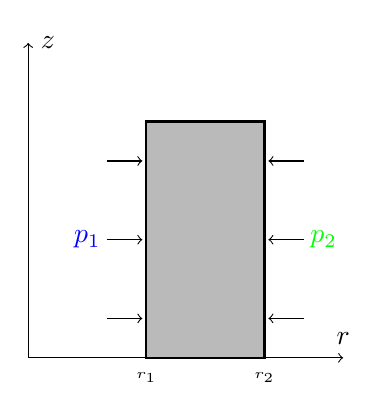
\begin{tikzpicture}
%\draw[fill=gray!23,gray!23](0,0) rectangle (6,5);
%\draw[step=0.5cm,gray,very thin] (0,0) grid (6,5); %background grid
\draw[thick,fill=gray!54] (2.5,.5)--(4,.5)--(4,3.5)--(2.5,3.5) -- cycle;

\draw[thin,->] (1,0.5) -- (5,0.5); %x
\draw[thin,->] (1,0.5) -- (1,4.5); %y
\node[] at (5,0.75) {$r$};
\node[] at (1.25,4.5) {$z$};

\node[] at (2.5,0.25) {\tiny $r_1$};
\node[] at (4,0.25) {\tiny $r_2$};

\draw[thin,->] (2,1) -- (2.45,1);
\draw[thin,->] (2,2) -- (2.45,2);
\draw[thin,->] (2,3) -- (2.45,3);

\draw[thin,->] (4.5,1) -- (4.05,1);
\draw[thin,->] (4.5,2) -- (4.05,2);
\draw[thin,->] (4.5,3) -- (4.05,3);

\node[] at (1.75,2) {\color{blue} $p_1$};
\node[] at (4.75,2) {\color{green} $p_2$};
\end{tikzpicture}
\end{center}

Because we have the analytical displacement field, we will be using it to 
impose Dirichlet boundary conditions on the sides, rather than pressure, and 
we will then recover strain and stress components.

Results for displacement, strain and stress as a function of $r$ are shown hereunder:
\begin{center}
\includegraphics[width=5.4cm]{python_codes/fieldstone_90/results/displacement.pdf}
\includegraphics[width=5.4cm]{python_codes/fieldstone_90/results/strain.pdf}
\includegraphics[width=5.4cm]{python_codes/fieldstone_90/results/stress.pdf}
\end{center}
The match is perfect and shows that the axisymmetric formulation presented in Section~\ref{ss:fem_elast_axis} is correct.

 %%%%%%%%%%%%%%%%%%%%%%%%%%%%%%%%%%%%%%%%%%%%%%%%%

\newpage %%%%%%%%%%%%%%%%%%%%%%%%%%%%%%%%%%%%%%%%%%%%%%%%%%%%%%%%%%%%%%%%%%%%%%%%%%%%%%%%
\section*{
Stone 91: Stokes sphere in a cylinder, axisymmetric formulation, $Q_2\times Q_1$
\label{f91}}
\addcontentsline{toc}{section}{\protect\numberline{} 
Stone 91: Stokes sphere in a cylinder, axisymmetric formulation, $Q_2\times Q_1$
}
Boundary conditions are: free slip on the left, top and bottom, and no slip on the right.

Having established the weak form of the Stokes equations and discretised them in 
Section~\ref{XXX}, transforming a 2D plane-strain code into an axisymmetric one is rather straightforward.
In a nutshell, 
\begin{itemize}
\item $x$ stands for r
\item $\upnu_r$ is $u$, $\upnu_z$ is $w$
\item the matrix ${\bm B}$ goes from 
$3 \times m_v\cdot ndofV$ to
$4 \times m_v\cdot ndofV$. 
\item the matrix ${\bm N}$ goes from 
$3 \times m_p\cdot ndofP$ to
$4 \times m_p\cdot ndofP$. 
\item the matrix ${\bm C}$ goes from 
$3 \times 3$ to $4 \times 4$.
\item integrals must be multiplied by $2 \pi$ and also contain an additional $r$ term
which translates into $x_q$ in the code. 
\end{itemize}


The Stokes sphere velocity is given by
\[
\upnu_{Stokes} = \frac{2}{9} \frac{\delta \rho}{\eta_f} R_s^2 g
\]
which yields $\upnu_S\simeq 3.387 \cdot 10^{-5}$. However, 
this is for a sphere in an infinite domain. When placed in a 
cylinder, the influence of the walls will slow the sphere down. 
Two corrections have been proposed be Habermann and by Faxen.

We start by writing the drag force
\[
F_H = 6 \pi \eta_f R \upnu_{sphere}  \gamma(r/R) 
\]
In the case of the Stokes sphere in an infinite medium then $\gamma =1$ and equating
$F_H$ with the buoyancy force $4/3 \pi R^3 \delta\rho g$ yields the above velocity.
Habermann gives a coefficient $\gamma$ such that 
\[
\gamma(r/R)  = \frac{1-0.75857 (r/R)^5}{1+f_H(r/R)}
\]
with 
\[
f_H(r/R) = -2.1050(r/R)+ 2.0865(r/R)^3-  1.7068(r/R)^5 + 0.72603(r/R)^6 
\]
Faxen gives a coefficient $\gamma$ such that 
\[
\gamma(r/R) = \frac{1}{1 + f_F(r/R)} 
\]
with 
\[
f_F(r/R) = -2.10444(r/R) + 2.08877(r/R)^3 - 0.94813(r/R)^5 -1.372(r/R)^6 + 3.87(r/R)^8 - 4.19(r/R)^{10}
\]
In all three cases we have 
\[
\upnu_{sphere} = \upnu_{Stokes} = \frac{2}{9} \frac{\delta \rho}{\eta_f} R_s^2 g \frac{1}{\gamma(r/R)}
\]
Note that the Habermann \& Faxen expressions are copy-pasted from the GALE manual. I did not verify these yet. 
Please check Lindgren (1999) \cite{lind99} to do so. They are about half the value of the Stokes velocity.

We see that increasing the height of the cylinder does not substantially alter the results, and that 
the velocity in the middle of the sphere seems to converge to the expected ones:
\begin{center}
\includegraphics[width=8cm]{python_codes/fieldstone_91/results/vc.pdf}
\includegraphics[width=8cm]{python_codes/fieldstone_91/results/mass.pdf}
{\captionfont up to 256x512 elements!}
\end{center}


\begin{center}
\includegraphics[width=4cm]{python_codes/fieldstone_91/results/ps/vel}
\includegraphics[width=4cm]{python_codes/fieldstone_91/results/ps/press}
\includegraphics[width=4cm]{python_codes/fieldstone_91/results/ps/exx}
\includegraphics[width=4cm]{python_codes/fieldstone_91/results/ps/exy}\\
\includegraphics[width=4cm]{python_codes/fieldstone_91/results/axi/vel}
\includegraphics[width=4cm]{python_codes/fieldstone_91/results/axi/press}
\includegraphics[width=4cm]{python_codes/fieldstone_91/results/axi/exx}
\includegraphics[width=4cm]{python_codes/fieldstone_91/results/axi/exy}\\
{\captionfont Top row: plane strain; Bottom row: axisymmetric. Resolution 50x100}
\end{center}


 %%%%%%%%%%%%%%%%%%%%%%%%%%%%%%%%%%%%%%%%%%%%%%%%%

\newpage %%%%%%%%%%%%%%%%%%%%%%%%%%%%%%%%%%%%%%%%%%%%%%%%%%%%%%%%%%%%%%%%%%%%%%%%%%%%%%%%
\section*{
Stone 92: Stokes sphere in a cylinder, axisymmetric formulation, $P_2^+\times P_{-1}$
\label{f92}}
\addcontentsline{toc}{section}{\protect\numberline{} 
Stone 92: Stokes sphere in a cylinder, axisymmetric formulation, $P_2^+\times P_{-1}$
}
\lstinputlisting[language=bash,basicstyle=\small]{python_codes/fieldstone_92/keywords}

\begin{center}
Code at \url{https://github.com/cedrict/fieldstone/tree/master/python_codes/fieldstone_92}
\end{center}

\par\noindent\rule{\textwidth}{0.4pt}

%%%%%%%%%%%%%%%%%%%%%%%%%%%%%%%%%%%%%%%%%%%%%%%%%%%%%%%%%%%%%%%%%%%%%%%%%%%%%%%%%%%%%%%%%%%%%%%%%%%%


This stone solves the axisymmetric problem of the Stokes sphere in a cylinder, 
similarly to Stone 91. However, it relies on an unstructured grid with 
Crouzeix-Raviart elements (see Section~\ref{ss:XXX}).

The workflow is as follows: the main parameters are defined in {\sl parameters.py}.
The file {\sl generate\_nodes.py} uses these parameters to generate points on the 
boundary of the rectangular domain and on the half circle. 
A call to {\sl triangle} is then made and a very important additional parameter is passed
as argument to triangle: the maximum area of a triangle. 
{\sl triangle} returns the (constrained) Delaunay triangulation of these points, 
and this information is then read in by {\sl stone.py} which solves the 
Stokes equation in axisymmetric formulation (see Section~\ref{ss:XXX}). 
Boundary conditions are free slip everywhere except no slip on the right. 

All these actions are carried out automatically when the following script is 
used\footnote{It assumes that the triangle program has been compiled and 
is located outside of the fieldstone tree.}:
\begin{lstlisting}
python3 generate_nodes.py
cat mypoints mysegments > mesh.poly
../../../../triangle/triangle  -j -q -a0.00100 -o2 -pc mesh.poly
echo "nel="
head -1 mesh.1.ele 
head -1 mesh.1.ele > temp
echo "NV0="
head -1 mesh.1.node 
head -1 mesh.1.node >> temp
python3 stone.py
\end{lstlisting}

Two remarks: the code stems from another code which implemented time stepping, 
which explains there is now a single fake time step loop in it. 
Pressure normalisation is not done the right way: the pressure nullspace is 
not removed from the matrix, but the solution is later normalised so that 
its average over the domain is zero.

\begin{center}
\includegraphics[width=4.3cm]{python_codes/fieldstone_92/results/mesh1}
\includegraphics[width=4.3cm]{python_codes/fieldstone_92/results/mesh2}
\includegraphics[width=4.3cm]{python_codes/fieldstone_92/results/mesh3}
\includegraphics[width=4.3cm]{python_codes/fieldstone_92/results/mesh4}\\
{\captionfont Left to right: nel=2432,2468,2588,2866}
\end{center}


\begin{center}
\includegraphics[width=5.5cm]{python_codes/fieldstone_92/results/mat}
\includegraphics[width=5.5cm]{python_codes/fieldstone_92/results/area}
\includegraphics[width=5.5cm]{python_codes/fieldstone_92/results/vel}\\
\includegraphics[width=5.5cm]{python_codes/fieldstone_92/results/u}
\includegraphics[width=5.5cm]{python_codes/fieldstone_92/results/v}
\includegraphics[width=5.5cm]{python_codes/fieldstone_92/results/press}\\
\includegraphics[width=5.5cm]{python_codes/fieldstone_92/results/sr}
\includegraphics[width=5.5cm]{python_codes/fieldstone_92/results/tauxx}
\includegraphics[width=5.5cm]{python_codes/fieldstone_92/results/tauxy}
\end{center}

Because the triangle size varies a lot within a mesh, defining a mesh size $h$
makes littel sense, so we plot the following results as a function of the 
number of elements:

\begin{center}
\includegraphics[width=8cm]{python_codes/fieldstone_92/results/vrms}
\includegraphics[width=8cm]{python_codes/fieldstone_92/results/vc}\\
{\captionfont Left: vrms over the whole domain for $L_y=1$; Right: 
measured velocity in the middle of the sphere.}
\end{center}

The parameter $n_p$ is user defined and is an attempt to parameterise 
the resolution of the domain sides and the half circle with a single parameter.
In {\sl parameters.py} we have:
\begin{lstlisting}
np_top=n_p
np_bottom=n_p
np_left=10*n_p
np_right=5*n_p
np_sphere=10*n_p
\end{lstlisting}

We see that the sphere velocity in its middle 
matches the Habermann and Faxen values remarkably well, 
especially when the domain is made taller (top and bottom 
boundaries are further away) and the viscosity of the 
sphere is brought up to $10^5$.


\begin{center}
\includegraphics[width=8cm]{python_codes/fieldstone_92/results/stress.png}
\includegraphics[width=8cm]{python_codes/fieldstone_92/results/theta.png}\\
{\captionfont Deviatoric stress principal directions (left) and angle (right).} 
\end{center}
 %%%%%%%%%%%%%%%%%%%%%%%%%%%%%%%%%%%%%%%%%%%%%%%%%

\newpage %%%%%%%%%%%%%%%%%%%%%%%%%%%%%%%%%%%%%%%%%%%%%%%%%%%%%%%%%%%%%%%%%%%%%%%%%%%%%%%%
\section*{
Stone 93: Buoyancy-driven flow with $P_2^+\times P_{-1}$
\label{f93}}
\addcontentsline{toc}{section}{\protect\numberline{} 
Stone 93: Buoyancy-driven flow with $P_2^+\times P_{-1}$
}
\lstinputlisting[language=bash,basicstyle=\small]{python_codes/fieldstone_93/keywords}

\begin{center}
Code at \url{https://github.com/cedrict/fieldstone/tree/master/python_codes/fieldstone_93}
\end{center}

\par\noindent\rule{\textwidth}{0.4pt}

%%%%%%%%%%%%%%%%%%%%%%%%%%%%%%%%%%%%%%%%%%%%%%%%%%%%%%%%%%%%%%%%%%%%%%%%%%%%%%%%%%%%%%%%%%%%%%%%%%%%


This stone solves the problem of the Stokes sphere sinking under a deformable free surface, 
It relies on an unstructured grid with Crouzeix-Raviart elements (see Section~\ref{ss:XXX}).

The workflow is as follows: the main parameters are defined in {\sl parameters.py}.
The file {\sl generate\_nodes.py} uses these parameters to generate points on the 
boundary of the rectangular domain, on the surface and on the circle and its center. 
A call to {\sl triangle} is then made and a very important additional parameter is passed
as argument to triangle: the maximum area of a triangle. 
{\sl triangle} returns the (constrained) Delaunay triangulation of these points, 
and this information is then read in by {\sl stone.py} which solves the 
Stokes equation. 
Boundary conditions are free slip everywhere. This benchmark is described in 
Section~\ref{ss:stokes_sphere_fs2D}.

All these actions are carried out automatically when the following script is 
used\footnote{It assumes that the triangle program has been compiled and 
is located outside of the fieldstone tree.}:
\begin{lstlisting}
python3 generate_nodes.py
cat mypoints mysegments > mesh.poly
../../../../triangle/triangle  -j -q -a0.00100 -o2 -pc mesh.poly
echo "nel="
head -1 mesh.1.ele 
head -1 mesh.1.ele > temp
echo "NV0="
head -1 mesh.1.node 
head -1 mesh.1.node >> temp
python3 stone.py
\end{lstlisting}


Note that ressure normalisation is not done the right way: the pressure nullspace is 
not removed from the matrix, but the solution is later normalised at the top
of the domain so that its average over the domain is zero.

Time stepping is carried out and the time step $\delta t$ is computed with a CFL criterion.
Nodes are advected with their velocity but no remeshing is implemented so that when the 
deformation becomes to large around the sphere the triangles become really deformed and 
the simulation must be stopped. Given the parameters of this benchmark this corresponds 
to $t\simeq 30$, while the simulation should ideally have been run up to $t>100$.

Nodes on the deformable surface are flagged at the beginning of the calculations and 
exported to an ascii file for later postprocessing. The multiple measurements for this 
benchmark are thoroughly described and plotted in Section~\ref{ss:stokes_sphere_fs2D}.


\begin{center}
\includegraphics[width=6.5cm]{python_codes/fieldstone_93/50/mesh0000}
\includegraphics[width=6.5cm]{python_codes/fieldstone_93/50/mesh0136}\\
\includegraphics[width=5.5cm]{python_codes/fieldstone_93/50/meshzoom0000}
\includegraphics[width=5.5cm]{python_codes/fieldstone_93/50/meshzoom0136}\\
{\captionfont  Mesh obtained with -a0.00050 in script}
\end{center}

\begin{center}
\includegraphics[width=5.5cm]{python_codes/fieldstone_93/results/mesh1}
\includegraphics[width=5.5cm]{python_codes/fieldstone_93/results/mesh2}
\includegraphics[width=5.5cm]{python_codes/fieldstone_93/results/mesh3}\\
{\captionfont  Mesh obtained with -a0.00050, -a0.00025 and -a0.00005 in script}
\end{center}

\begin{center}
\includegraphics[width=4cm]{python_codes/fieldstone_93/results/vel_0000}
\includegraphics[width=4cm]{python_codes/fieldstone_93/results/p_0000}
\includegraphics[width=4cm]{python_codes/fieldstone_93/results/sr_0000}
\includegraphics[width=4cm]{python_codes/fieldstone_93/results/mat_0000}\\
\includegraphics[width=4cm]{python_codes/fieldstone_93/results/vel_0136}
\includegraphics[width=4cm]{python_codes/fieldstone_93/results/p_0136}
\includegraphics[width=4cm]{python_codes/fieldstone_93/results/sr_0136}
\includegraphics[width=4cm]{python_codes/fieldstone_93/results/mat_0136}\\
{\captionfont  Mesh obtained with -a0.00025 in script. Top row $t=0$, 
bottom row $t\simeq 30$.}
\end{center}


\newpage

\begin{center}
\includegraphics[width=5.7cm]{python_codes/fieldstone_93/results/vrms}
\includegraphics[width=5.7cm]{python_codes/fieldstone_93/results/vrms_sphere}
\includegraphics[width=5.7cm]{python_codes/fieldstone_93/results/vrms_fluidsphere}\\
\includegraphics[width=7cm]{python_codes/fieldstone_93/results/p_bottom}
\includegraphics[width=7cm]{python_codes/fieldstone_93/results/max_vel}\\
\includegraphics[width=5.7cm]{python_codes/fieldstone_93/results/max_press}
\includegraphics[width=5.7cm]{python_codes/fieldstone_93/results/avrg_density}
\includegraphics[width=5.7cm]{python_codes/fieldstone_93/results/avrg_viscosity}\\
\includegraphics[width=7cm]{python_codes/fieldstone_93/results/center_position_x}
\includegraphics[width=7cm]{python_codes/fieldstone_93/results/center_position_y}\\
\includegraphics[width=7cm]{python_codes/fieldstone_93/results/center_velocity_x}
\includegraphics[width=7cm]{python_codes/fieldstone_93/results/center_velocity_y}\\
\includegraphics[width=7cm]{python_codes/fieldstone_93/results/topography_min}
\includegraphics[width=7cm]{python_codes/fieldstone_93/results/topography_max}\\
\includegraphics[width=5.7cm]{python_codes/fieldstone_93/results/point_u}
\includegraphics[width=5.7cm]{python_codes/fieldstone_93/results/point_v}
\includegraphics[width=5.7cm]{python_codes/fieldstone_93/results/point_p}\\
\includegraphics[width=5.7cm]{python_codes/fieldstone_93/results/dt}
\includegraphics[width=5.7cm]{python_codes/fieldstone_93/results/vol_sphere}
\includegraphics[width=5.7cm]{python_codes/fieldstone_93/results/vol_fluidsphere}
\end{center}

Results are remarkably similar for all resolutions. Note that because the pressure 
is discontinuous across element edges, the recorded value at (0.5,0.6) shows small
jumps.













 %%%%%%%%%%%%%%%%%%%%%%%%%%%%%%%%%%%%%%%%%%%%%%%%%

\newpage %%%%%%%%%%%%%%%%%%%%%%%%%%%%%%%%%%%%%%%%%%%%%%%%%%%%%%%%%%%%%%%%%%%%%%%%%%%%%%%%
\section*{
Stone 94: visualising UUP07 in Paraview
\label{f94}}
\addcontentsline{toc}{section}{\protect\numberline{} 
Stone 94: visualising UUP07 in Paraview
}
\lstinputlisting[language=bash,basicstyle=\small]{python_codes/fieldstone_94/keywords}

\begin{center}
Code at \url{https://github.com/cedrict/fieldstone/tree/master/python_codes/fieldstone_94}
\end{center}

\par\noindent\rule{\textwidth}{0.4pt}

{\sl This stone was developed in collaboration with Lex Verbrugh}. \index{contributors}{L. Verbrugh}

\par\noindent\rule{\textwidth}{0.4pt}

%%%%%%%%%%%%%%%%%%%%%%%%%%%%%%%%%%%%%%%%%%%%%%%%%%%%%%%%%%%%%%%%%%%%%%%%%%%%%%%%%%%%%%%%

This stone is a simple tool to visualise the UUP07 $V_p$ tomography model \cite{hasp15} in paraview. 
The data is available online at \url{https://www.atlas-of-the-underworld.org/downloads/}.
The file is 230Mb so it is not archived here. 
Simply download it and place in the same folder as the python file. 
The output can be either in a Cartesian domain or a hollow sphere of radius $6371\si{\kilo\metre}$.
Plates and continent lines obtained from Stone 69.

\begin{center}
\includegraphics[width=14cm]{python_codes/fieldstone_94/map} 
\end{center}


\begin{center}
\includegraphics[width=5.7cm]{python_codes/fieldstone_94/sphere1} 
\includegraphics[width=5.7cm]{python_codes/fieldstone_94/sphere2} 
\includegraphics[width=5.7cm]{python_codes/fieldstone_94/sphere3} 
\end{center}


 %%%%%%%%%%%%%%%%%%%%%%%%%%%%%%%%%%%%%%%%%%%%%%%%%

\newpage %%%%%%%%%%%%%%%%%%%%%%%%%%%%%%%%%%%%%%%%%%%%%%%%%%%%%%%%%%%%%%%%%%%%%%%%%%%%%%%%
\section*{
Stone 95: van Keken \etal Rayleigh-Taylor instability with $P_2^+\times P_{-1}$ and mesh adaptivity
\label{f95}}
\addcontentsline{toc}{section}{\protect\numberline{} 
Stone 95: van Keken \etal Rayleigh-Taylor instability with $P_2^+\times P_{-1}$ and mesh adaptivity
}
\lstinputlisting[language=bash,basicstyle=\small]{python_codes/fieldstone_95/keywords}

\begin{center}
Code at \url{https://github.com/cedrict/fieldstone/tree/master/python_codes/fieldstone_95}
\end{center}

\par\noindent\rule{\textwidth}{0.4pt}

%%%%%%%%%%%%%%%%%%%%%%%%%%%%%%%%%%%%%%%%%%%%%%%%%%%%%%%%%%%%%%%%%%%%%%%%%%%%%%%%%%%%%%%%

This stone tackles the Rayleigh-Taylor instability problem of van Keken \etal \cite{vaks97}. 
It builds on Stone 93 as it relies on triangular elements (the MINI element(see Section~\ref{pair:mini}), 
the Taylor-Hood $P_2\times P_1$ element (see Section~\ref{ss:p2p1}), 
and the Crouzeix-Raviart element (see Section~\ref{sec:crouzeix-raviart})) and Delaunay meshes
generated by the Triangle code \cite{shew14}.  

However, this code does implements mesh adaptation and the python code then calls the Triangle mesher code
at every timestep (the remeshing cost is negligible).
I unfortunately cannot prevent Triangle from adding nodes in between the interface nodes, thereby 
ruining the numbering and the flagging of these nodes. I have therefore implemented a refinement 
process which add nodes on the interface when two consecutive nodes are getting too far apart (which 
would have been necessary because of the shear stretching of the interface). 

\begin{center}
\includegraphics[width=5.5cm]{python_codes/fieldstone_95/init/mat}
\includegraphics[width=5.5cm]{python_codes/fieldstone_95/init/interface}
\includegraphics[width=5.5cm]{python_codes/fieldstone_95/init/area}\\
{\captionfont Interface counts 100 points, Triangle argument a=0.001, } 
\end{center}

The number of parameters one can vary is somewhat limited:
\begin{itemize}
\item the CFL number - default 0.25 (note that the time step is limited to 0.5);
\item the maximum area $a$ of triangles (passed as argument to Triangle) - default 0.001 for second order elements,
0.0005 of first order element;
\item the initial number of triangle vertices on the interface $np_{surf}$ - default 200;
\item the stretch factor controlling the addition of points $\gamma$ - default 1.5;
\item the type of element (element 1: MINI, element 2: Crouzeix-Raviart, element 3: Taylor-Hood)  
\end{itemize}

I also somewhat arbitrarily set the timestep to be limited to $\delta t_{\rm max}=0.25$. This allows for accurate 
measurements of the growth rate across all models. 
In the end we wish to plot the time evolution of the root mean square velocity and 
establish the time and amplitude of the first two peaks. We also wish to monitor volume/mass conservation.  

\newpage
%..........................................................
\subsubsection*{Isoviscous results - instantaneous results}.

\begin{center}
\begin{tabular}{|l|l|l|l|l|l|l|l|}
\hline
                & $a=0.002$     & $a=0.001$    & a=0.0008     & $a=0.0005$    & a=0.0004     & $a=0.0003$ & $a=0.0002$ \\ \hline
$np_{surf}$=150 &               &              &              & 1.852875e-04  & 1.852877e-04 & & \\ \hline
$np_{surf}$=200 & 1.852812e-04  & 1.852888e-04 & 1.852900e-04 & 1.852904e-04  & 1.852907e-04 & & \\ \hline
$np_{surf}$=250 &               &              &              & 1.852919e-04  & 1.852922e-04 & & \\ \hline
$np_{surf}$=300 &               &              &              & 1.852926e-04  & 1.852929e-04 & 1.852930e-04 & \\ \hline
$np_{surf}$=350 & 1.852838e-04  & 1.852916e-04 & 1.852924e-04 & 1.852932e-04  & 1.852933e-04 & 1.852936e-04 & \\ \hline
$np_{surf}$=400 & 1.852816e-04  & 1.852922e-04 & 1.852928e-04 & 1.852934e-04  & 1.852936e-04 & 1.852938e-04 & 1.852940e-04 \\ \hline
$np_{surf}$=450 & 1.852851e-04  & 1.852920e-04 & 1.852928e-04 & 1.852937e-04  & 1.852939e-04 & 1.852940e-04 & 1.852942e-04 \\ \hline
$np_{surf}$=500 & 1.852852e-04  & 1.852928e-04 & 1.852935e-04 & 1.852938e-04  & 1.852940e-04 & 1.852942e-04 & 1.852943e-04 \\ \hline
$np_{surf}$=550 &               &              &              & 1.852939e-04  & 1.852942e-04 & 1.852943e-04 & 1.852944e-04 \\ \hline
\end{tabular} \\
{\captionfont
Root mean square velocity $v_{rms}$ value for $t=0$. Crouzeix-Raviart element.}
\end{center}

%..........................................................
\subsubsection*{Isoviscous results - short term}

We now turn to the growth rate(s) which is measured in gnuplot as follows:

\begin{verbatim}
f(x)=a*exp(b*x)
fit f(x) 'benchmark_default.ascii' u 3:(($23-$21)) via a,b
\end{verbatim}

\begin{center}
\includegraphics[width=5.5cm]{python_codes/fieldstone_95/results/growth_rate}
\includegraphics[width=5.5cm]{python_codes/fieldstone_95/results/growth_rate_vrms}
\includegraphics[width=5.5cm]{python_codes/fieldstone_95/results/growth_rate_maxv}
\end{center}


\begin{center}
\begin{tabular}{llll}
\hline
model    & $\gamma(h)$ & $\gamma(v_{rms})$ & $\gamma(\max(v))$ \\
\hline
\hline
default                 & 0.0108964 & 0.0110335& 0.0132341 \\
def. w/ $np_{surf}$=250 & 0.0108964 & 0.0110438& 0.0132409\\
def. w/ $np_{surf}$=300 & 0.0108964 & 0.0110449& 0.0134468\\
def. w/ $np_{surf}$=400 & 0.0108964 & 0.0110454& 0.0132651\\  
def. w/ $a=0.0005$      & 0.0108964 & 0.0110449& 0.0133781\\
\hline
\end{tabular}
\end{center}

%..........................................................
\subsubsection*{Isoviscous results - Long term evolution}

The script {\tt script\_run\_al} is designed to run for a long time (several days) 
and will lauch all 1+14 runs at the same time: 

\begin{tabular}{lccccc}
\hline
experiment &  CFL   &  $a$   & $np_{surf}$ & $\gamma$ & elt type \\
\hline
\hline
default    &  0.25  &  0.001 & 200         & 1.5      &  2        \\
\#1        &  '     &    '   & 250         & '        &  '        \\
\#2        &  '     &    '   & 300         & '        &  '        \\
\#3        &  '     &    '   & 350         & '        &  '        \\
\#4        &  '     &    '   & 400         & '        &  '        \\
\#5        &  '     &    '   & 500         & '        &  '        \\
\#6        &  '     &    '   & '           & 1.25     &  '        \\
\#7        &  '     & 0.0008 & '           & '        &  '        \\
\#8        &  '     & 0.0005 & '           & '        &  '        \\
\#9        &  '     &    '   & '           & '        &  3        \\
\#10       &  '     & 0.0005 & 400         & '        &  '        \\
\#11       &  0.1   &    '   & '           & '        &  '        \\
\#12       &  0.5   &    '   & '           & '        &  '        \\
\#13       &  0.75  &    '   & '           & '        &  '        \\
\#14       &  1     &    '   & '           & '        &  '        \\
\hline
\end{tabular}

Results are shown hereunder:

\begin{itemize}
\item minimum and maximum value of the velocity components $u$ and $v$:

\begin{center}
\includegraphics[width=7.5cm]{python_codes/fieldstone_95/results/u}
\includegraphics[width=7.5cm]{python_codes/fieldstone_95/results/v}\\
\end{center}

\item max($v$) for the first 10 seconds:

\begin{center}
\includegraphics[width=7.5cm]{python_codes/fieldstone_95/results/v_start}
\end{center}

\item time step $\delta t$ value: 

\begin{center}
\includegraphics[width=7.5cm]{python_codes/fieldstone_95/results/dt}
\end{center}

\item volume of fluid 1 and 2 (relative change):

\begin{center}
\includegraphics[width=7.5cm]{python_codes/fieldstone_95/results/vol1}
\includegraphics[width=7.5cm]{python_codes/fieldstone_95/results/vol2}
\end{center}

\item number of elements: 

\begin{center}
\includegraphics[width=7.5cm]{python_codes/fieldstone_95/results/nel}
\end{center}

\item velocity norm $|\vec\upnu|$
 
\begin{center}
\includegraphics[width=7.5cm]{python_codes/fieldstone_95/results/vel}
\end{center}

\item The root mean square velocity

\begin{center}
\includegraphics[width=7.5cm]{python_codes/fieldstone_95/results/vrms2000}
\includegraphics[width=7.5cm]{python_codes/fieldstone_95/results/vrms400}\\
\includegraphics[width=7.5cm]{python_codes/fieldstone_95/results/vrms_peak1}
\includegraphics[width=7.5cm]{python_codes/fieldstone_95/results/vrms_peak2}\\
\end{center}

\item the number of points on the interface
and its length 

\begin{center}
\includegraphics[width=5.5cm]{python_codes/fieldstone_95/results/np_surf}
\includegraphics[width=5.5cm]{python_codes/fieldstone_95/results/length_interface}
\end{center}

\item the position of interseaction of the interface with the left and right boundaries: 

\begin{center}
\includegraphics[width=5.5cm]{python_codes/fieldstone_95/results/left}
\includegraphics[width=5.5cm]{python_codes/fieldstone_95/results/right}
\end{center}

\end{itemize}




%\begin{center}
%\includegraphics[width=5.5cm]{python_codes/fieldstone_95/results/npsurf250/grid0000.png}
%\includegraphics[width=5.5cm]{python_codes/fieldstone_95/results/npsurf250/grid0050.png}
%\includegraphics[width=5.5cm]{python_codes/fieldstone_95/results/npsurf250/grid0100.png}\\
%\includegraphics[width=5.5cm]{python_codes/fieldstone_95/results/npsurf250/grid0150.png}
%\includegraphics[width=5.5cm]{python_codes/fieldstone_95/results/npsurf250/grid0200.png}
%\includegraphics[width=5.5cm]{python_codes/fieldstone_95/results/npsurf250/grid0250.png}\\
%\includegraphics[width=5.5cm]{python_codes/fieldstone_95/results/npsurf250/grid0300.png}
%\includegraphics[width=5.5cm]{python_codes/fieldstone_95/results/npsurf250/grid0350.png}
%\includegraphics[width=5.5cm]{python_codes/fieldstone_95/results/npsurf250/grid0400.png}\\
%{\captionfont Cade default + npsurf=250, up to time = 400}
%\end{center}


I have also plotted the vrms against those of the original paper and those of Louis-Napoleon \etal \cite{logb20}
(with codes JADIM and OpenFOAM). 
The main parameter which seems to govern overal mass/volume conservation is the resolution of the interface. 

QUESTION: at the end of the first time step, when I write down the time associated with the measurements, should I write 0
or dt ?

QUESTION: does reduced density use change results ?

TODO: run until time=1500

TODO: viscosity ratio 10 and 100 cases

 %%%%%%%%%%%%%%%%%%%%%%%%%%%%%%%%%%%%%%%%%%%%%%%%%

\newpage %%%%%%%%%%%%%%%%%%%%%%%%%%%%%%%%%%%%%%%%%%%%%%%%%%%%%%%%%%%%%%%%%%%%%%%%%%%%%%%%
\section*{
Stone 96: honours project 
\label{f96}}
\addcontentsline{toc}{section}{\protect\numberline{} 
Stone 96: honours project 
}


Facts about planet Mars\footnote{\url{https://en.wikipedia.org/wiki/Mars}}:
\begin{itemize}
\item average radius $R=3389.5 \pm 0.2 \si{\km}$
\item equatorial radius $3396.2 \pm 0.1 \si{\km}$
\item polar radius $3376.2 \pm 0.1 \si{\km}$
\item volume $1.6318 \cdot 10^{20} \si{\cubic\metre}$
\item mass $6.4171 \cdot 10^{23}\si{\kilo\gram}$
\item mean density $\langle\rho\rangle= 3934\si{\kilo\gram\per\cubic\meter}$
\item moment of inertia $I=0.3644 \pm 0.0005$
\item surface gravity $g=3.72076 \si{\metre\per\square\second}$
\end{itemize}

The surface gravity can be obtained with 
\[
g_{surf}=\frac{{\cal G} M}{R^2} 
=\frac{6.67430 \cdot 10^{-11} \; 6.4171 \cdot 10^{23} }{(3.3895\cdot 10^6)^2}
\simeq 3.727977
\]

The internal structure of the planet is not settled although 
it is now widely accepted that the planet has a core. 

B. Steinberger was kind enough to communicate to us the density and viscosity 
profiles used in Steinverger \etal (2010) \cite{stwt10} \footnote{Files sent to us 
we slightly altered for the purpose of this work. The density profile was missing 
the 50km near the center of the planet so padding was used. The viscosity profile 
starts below the moho at 50\si{\km} and stopped at the cmb. }:

\begin{center}
\includegraphics[width=7cm]{python_codes/fieldstone_96/data/rho1}
\includegraphics[width=7cm]{python_codes/fieldstone_96/data/eta1}\\
\includegraphics[width=7cm]{python_codes/fieldstone_96/data/rho2}
\includegraphics[width=7cm]{python_codes/fieldstone_96/data/eta2}\\
{\captionfont Data curtesy of B. Steinberger, from \cite{stwt10}} \\
{\tiny {\color{gray} in python\_codes/fieldstone\_96/data/}}
\end{center}


\begin{center}
\includegraphics[width=5.7cm]{python_codes/fieldstone_96/images/stwt10_b}
\includegraphics[width=5.7cm]{python_codes/fieldstone_96/images/stwt10_c}
\includegraphics[width=5.7cm]{python_codes/fieldstone_96/images/stwt10_d}\\
{\captionfont Taken from Steinverger \etal (2010) \cite{stwt10}}
\end{center}

In table 1 of Steinberger \etal \cite{stwt10}: crust thickness is set to 50km. The core radius is set 
to 1389.5km. However in the data set we were sent it seems that the cmb is at 1422\si{\km}
radius.
To simplify things we take $R=3389\si{\km}$ and $R_{cmb}=1422\si{\km}$ in the code.

There are three python files in this \stone:
\begin{itemize}
\item {\pythonfile parameters.py}: the main physical and geometrical parameters are defined in it;
\item {\pythonfile generate\_nodes.py}: this code generates the two files  {\sl mypoints} and {\sl mysegments}
which will be first concatenated into {\sl mesh.poly} and then passed to the Triangle mesher. 
The mesher then returns {\sl mesh.1.node} and {\sl mesh.1.ele}.  
\item {\pythonfile stone.py} This is the 'real' code: the above mentioned files are read in and are used to 
build the mesh. Density and viscosity profile datasets are read in so that viscosity, density and 
gravity acceleration can then be assigned to elements/nodes/quadrature points. Boundary conditions 
are set up, the FEM is built, and the system solved. The pressure at the surface of the planet is 
normalised to zero average. Results are then exported to ascii and vtu file(s).
\end{itemize}
In order to run the code, simply make use of the provided script {\shellscriptfile run\_script}. 
In it the call to the Triangle mesher is carried out:
\begin{verbatim}
../../../../triangle/triangle   -q -j -O -a4000000000 -o2 -pc  mesh.poly
\end{verbatim}
The number following the {\tt -a} option is the maximum size of an element. This controls the 
average size of the generated elements inside the domain. Decreasing this number automatically 
generates more elements, i.e. a higher resolution. 

\begin{center}
\begin{flushright} {\tiny {\color{gray} (tikz\_axi.tex)}} \end{flushright}
%~~~~~~~~~~~~~~~~~~~~~~~~~~~~~~~~~~~~~~~~~~~~~~~~~~~~~~~~~~~~~~~~~~~~~~~~~~~~~~~~~~~~~~~~~~~~~~~~~~

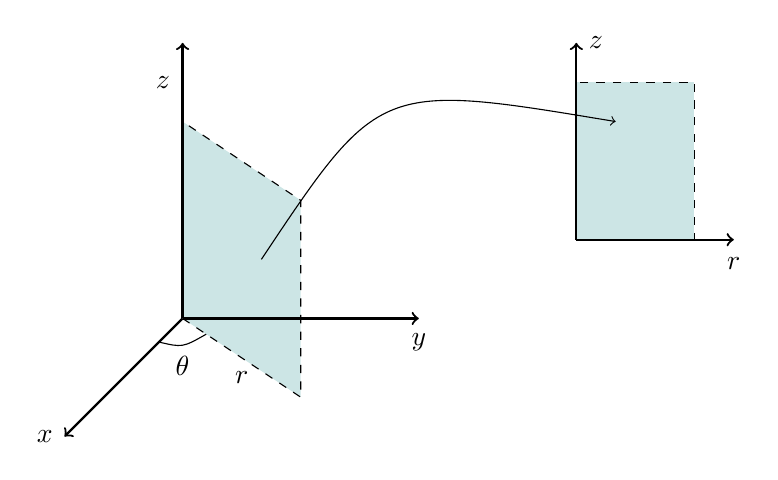
\begin{tikzpicture}
%\draw[step=0.5cm,gray,very thin] (0,0) grid (10,6); %background grid

\draw[dashed,fill=teal!20] (2,2)--(3.5,1)--(3.5,3.5)--(2,4.5)--cycle ;
\draw[thick,->] (2,2) -- (0.5,0.5); 
\draw[thick,->] (2,2) -- (5,2); 
\draw[thick,->] (2,2) -- (2,5.5); 
\node[] at (0.25,0.5) {$x$};
\node[] at (5,1.7) {$y$};
\node[] at (1.75,5) {$z$};
\node[] at (2.75,1.25) {$r$};
\node[] at (2,1.4) {$\theta$};
\draw[] (1.7,1.7) .. controls (2,1.63) ..   (2.3,1.8);

\draw[dashed,fill=teal!20] (7,3)--(8.5,3)--(8.5,5)--(7,5)--cycle; 
\draw[thick,->] (7,3) -- (9,3); 
\draw[thick,->] (7,3) -- (7,5.5); 
\node[] at (9,2.7) {$r$};
\node[] at (7.25,5.5) {$z$};

\draw[->] (3,2.75) .. controls (4.5,5) .. (7.5,4.5);
\end{tikzpicture}



\end{center}

\begin{center}
\includegraphics[width=7cm]{python_codes/fieldstone_96/images/notes1}\\
\includegraphics[width=9cm]{python_codes/fieldstone_96/images/notes2}
\end{center}

Given the symmetry of the problem any term containing $\partial_\theta$ or $\upnu_\theta$ is zero.
The strain rate tensor given in Section~\ref{ss:srcc} then simplifies to:

\begin{eqnarray}
\dot\varepsilon_{rr} 
&=& \frac{\partial \upnu_r}{\partial r} \nn\\
\dot\varepsilon_{\theta\theta}  &=& \frac{\upnu_r}{r} \nn\\
\dot\varepsilon_{\theta r} = \dot\varepsilon_{r\theta}  &=& 0 \nn\\
\dot\varepsilon_{zz} &=& \frac{\partial \upnu_z}{\partial z} \nn\\
\dot{\varepsilon}_{rz} = \dot{\varepsilon}_{zr} 
&=& \frac{1}{2}\left( \frac{\partial \upnu_r}{\partial z} + \frac{\partial \upnu_z}{\partial r} \right) \nn\\
\dot{\varepsilon}_{\theta z} = \dot{\varepsilon}_{z \theta} &=& 0 \nn
\end{eqnarray}
Note that the term $\dot\varepsilon_{\theta\theta} $ is not zero!
The deviatoric stress tensor ${\bm \tau}=2\eta \dot{\bm \varepsilon}$ can be computed
as well as the full stress tensor ${\bm \sigma}=-p {\bm 1} + {\bm \tau}$. 

\begin{center}
\includegraphics[width=6cm]{python_codes/fieldstone_96/images/rho}
\includegraphics[width=6cm]{python_codes/fieldstone_96/images/eta}
\includegraphics[width=6cm]{python_codes/fieldstone_96/images/mesh}
\end{center}

%--------------------------------------------------
\subsubsection*{Stresses and coordinate changes}

\paragraph{From Cylindrical to Cartesian coordinates}

In cylindrical coordinates, and in the axisymmetric case
the strain rate tensor is given by
\[
\dot{\bm\varepsilon}
=
\left(
\begin{array}{ccc}
\dot\varepsilon_{rr} & 0 & \dot{\varepsilon}_{rz} \\
0 & \dot{\varepsilon}_{\theta\theta}  & 0 \\
\dot{\varepsilon}_{zr} & 0 & \dot\varepsilon_{zz}
\end{array}
\right)
\]
We will now convert it to Cartesian coordinates using the equation from \url{https://www.brown.edu/Departments/Engineering/Courses/En221/Notes/Polar_Coords/Polar_Coords.htm}:
\[
{\bm T}_{\tiny Cyl}=
\left(
\begin{array}{ccc}
T_{rr}       & T_{r\theta}      & T_{rz} \\
T_{\theta r} & T_{\theta\theta} & T_{\theta z} \\
T_{z r}      & T_{z \theta}     & T_{zz}
\end{array}
\right)
=
\left(
\begin{array}{ccc}
 \cos \theta&\sin \theta&0 \\
-\sin \theta&\cos \theta&0 \\
0 & 0 & 1 
\end{array}
\right)
\cdot
\left(
\begin{array}{ccc}
T_{xx} & T_{xy} & T_{xz} \\
T_{yx} & T_{yy} & T_{yz} \\
T_{zx} & T_{zy} & T_{zz} 
\end{array}
\right)
\cdot
\left(
\begin{array}{ccc}
\cos \theta & -\sin \theta&0 \\
\sin \theta &  \cos \theta&0 \\
0 & 0 & 1 
\end{array}
\right)
\]

\[
{\bm T}_{\tiny Cart}=
\left(
\begin{array}{ccc}
T_{xx} & T_{xy} & T_{xz} \\
T_{yx} & T_{yy} & T_{yz} \\
T_{zx} & T_{zy} & T_{zz} 
\end{array}
\right)
=
\left(
\begin{array}{ccc}
 \cos \theta&-\sin \theta&0 \\
\sin \theta&\cos \theta&0 \\
0 & 0 & 1 
\end{array}
\right)
\cdot
\left(
\begin{array}{ccc}
T_{rr}       & T_{r\theta}      & T_{rz} \\
T_{\theta r} & T_{\theta\theta} & T_{\theta z} \\
T_{z r}      & T_{z \theta}     & T_{zz}
\end{array}
\right)
\cdot
\left(
\begin{array}{ccc}
\cos \theta & \sin \theta&0 \\
-\sin \theta &  \cos \theta&0 \\
0 & 0 & 1 
\end{array}
\right)
\]
In our case the calculation is taking place in the $(x,z)$
plane, i.e. $\theta=0$ so that the rotation matrices above 
are in fact identity matrices. 
We then simply have 
$\dot{\bm \varepsilon}_{\tiny Cart}=
\dot{\bm \varepsilon}_{\tiny Cyl}$.



%..........................................................
\paragraph{From Cartesian to Spherical coordinates}

We have
\[
{\bm T}_{\tiny Sph}=
\left(
\begin{array}{ccc}
T_{rr}       & T_{r\theta}      & T_{r\phi} \\
T_{\theta r} & T_{\theta\theta} & T_{\theta\phi} \\
T_{\phi r}   & T_{\phi \theta}  & T_{\phi\phi}
\end{array}
\right)
=
\left(
\begin{array}{ccc}
\sin\theta \cos\phi & \sin\theta \sin\phi & \cos\theta \\
\cos\theta \cos\phi & \cos\theta \sin\phi & -\sin\theta \\
-\sin\phi & \cos\phi & 0 
\end{array}
\right)
\cdot
\left(
\begin{array}{ccc}
T_{xx} & T_{xy} & T_{xz} \\
T_{yx} & T_{yy} & T_{yz} \\
T_{zx} & T_{zy} & T_{zz} 
\end{array}
\right)
\cdot
\left(
\begin{array}{ccc}
\sin\theta\cos\phi & \cos\theta\cos\phi & -\sin\phi \\
\sin\theta\sin\phi & \cos\theta\sin\phi & \cos\phi \\
\cos\theta & -\sin\theta & 0
\end{array}
\right)
\]

\[
{\bm T}_{\tiny Cart}=
\left(
\begin{array}{ccc}
T_{xx} & T_{xy} & T_{xz} \\
T_{yx} & T_{yy} & T_{yz} \\
T_{zx} & T_{zy} & T_{zz} 
\end{array}
\right)
=
\left(
\begin{array}{ccc}
\sin\theta\cos\phi & \cos\theta\cos\phi & -\sin\phi \\
\sin\theta\sin\phi & \cos\theta\sin\phi & \cos\phi \\
\cos\theta & -\sin\theta & 0
\end{array}
\right)
\cdot
\left(
\begin{array}{ccc}
T_{rr}       & T_{r\theta}      & T_{r\phi} \\
T_{\theta r} & T_{\theta\theta} & T_{\theta\phi} \\
T_{\phi r}   & T_{\phi \theta}  & T_{\phi\phi}
\end{array}
\right)
\cdot
\left(
\begin{array}{ccc}
\sin\theta \cos\phi & \sin\theta \sin\phi & \cos\theta \\
\cos\theta \cos\phi & \cos\theta \sin\phi & -\sin\theta \\
-\sin\phi & \cos\phi & 0 
\end{array}
\right)
\]
In our case, calculations take place in the 
$(x,z)$-plane so we have $\phi=0$ and the equation above 
becomes
\[
\left(
\begin{array}{ccc}
T_{rr}       & T_{r\theta}      & T_{r\phi} \\
T_{\theta r} & T_{\theta\theta} & T_{\theta\phi} \\
T_{\phi r}   & T_{\phi \theta}  & T_{\phi\phi}
\end{array}
\right)
=
\left(
\begin{array}{ccc}
\sin\theta  & 0 & \cos\theta \\
\cos\theta  & 0 & -\sin\theta \\
0 & 1 & 0 
\end{array}
\right)
\cdot
\left(
\begin{array}{ccc}
T_{xx} & T_{xy} & T_{xz} \\
T_{yx} & T_{yy} & T_{yz} \\
T_{zx} & T_{zy} & T_{zz} 
\end{array}
\right)
\cdot
\left(
\begin{array}{ccc}
\sin\theta & \cos\theta & 0 \\
0 & 0 & 1 \\
\cos\theta & -\sin\theta & 0
\end{array}
\right)
\]
We define $c_\theta=\cos\theta$, $s_\theta=\sin\theta$ so that
\[
\left(
\begin{array}{ccc}
T_{rr}       & T_{r\theta}      & T_{r\phi} \\
T_{\theta r} & T_{\theta\theta} & T_{\theta\phi} \\
T_{\phi r}   & T_{\phi \theta}  & T_{\phi\phi}
\end{array}
\right)
=
\left(
\begin{array}{ccc}
s_\theta  & 0 & c_\theta \\
c_\theta  & 0 & -s_\theta \\
0 & 1 & 0 
\end{array}
\right)
\cdot
\left(
\begin{array}{ccc}
T_{xx} & T_{xy} & T_{xz} \\
T_{yx} & T_{yy} & T_{yz} \\
T_{zx} & T_{zy} & T_{zz} 
\end{array}
\right)
\cdot
\left(
\begin{array}{ccc}
s_\theta & c_\theta & 0 \\
0 & 0 & 1 \\
c_\theta & -s_\theta & 0
\end{array}
\right)
\]
As we have seen above we have 
\[
\dot{\bm\varepsilon}_{\tiny Cart}
=
\left(
\begin{array}{ccc}
\dot\varepsilon_{xx} & 0 & \dot{\varepsilon}_{xz} \\
0 & \dot{\varepsilon}_{yy}  & 0 \\
\dot{\varepsilon}_{xz} & 0 & \dot\varepsilon_{zz}
\end{array}
\right)
\]
so 
\begin{eqnarray}
\dot{\bm \varepsilon}_{\tiny Sph}=
\left(
\begin{array}{ccc}
\dot\varepsilon_{rr}       & \dot\varepsilon_{r\theta}      & \dot\varepsilon_{r\phi} \\
\dot\varepsilon_{\theta r} & \dot\varepsilon_{\theta\theta} & \dot\varepsilon_{\theta\phi} \\
\dot\varepsilon_{\phi r}   & \dot\varepsilon_{\phi \theta}  & \dot\varepsilon_{\phi\phi}
\end{array}
\right)
&=&
\left(
\begin{array}{ccc}
s_\theta  & 0 & c_\theta \\
c_\theta  & 0 & -s_\theta \\
0 & 1 & 0 
\end{array}
\right)
\cdot
\left(
\begin{array}{ccc}
\dot\varepsilon_{xx} & 0 & \dot{\varepsilon}_{xz} \\
0 & \dot{\varepsilon}_{yy}  & 0 \\
\dot{\varepsilon}_{xz} & 0 & \dot\varepsilon_{zz}
\end{array}
\right)
\cdot
\left(
\begin{array}{ccc}
s_\theta & c_\theta & 0 \\
0 & 0 & 1 \\
c_\theta & -s_\theta & 0
\end{array}
\right)  \nonumber\\
&=&
\left(
\begin{array}{ccc}
s_\theta  & 0 & c_\theta \\
c_\theta  & 0 & -s_\theta \\
0 & 1 & 0 
\end{array}
\right)
\cdot
\left(
\begin{array}{ccc}
\dot\varepsilon_{xx} s_\theta + 
\dot\varepsilon_{xz} c_\theta  & 
\dot\varepsilon_{xx} c_\theta - 
\dot\varepsilon_{xz} s_\theta  &
0 \\
0 & 0 & \dot{\varepsilon}_{yy}  
\\
\dot\varepsilon_{xz} s_\theta + 
\dot\varepsilon_{zz} c_\theta  &
\dot\varepsilon_{xz} c_\theta - 
\dot\varepsilon_{zz} s_\theta  &
0 
\end{array}
\right)  \nonumber\\
&=&
\left(
\begin{array}{ccc}
\dot\varepsilon_{xx} s_\theta^2 + 
2 \dot\varepsilon_{xz} c_\theta  s_\theta +
\dot\varepsilon_{zz} c_\theta ^2  
& 
\dot\varepsilon_{xx} c_\theta s_\theta - 
\dot\varepsilon_{xz} s_\theta^2  +
\dot\varepsilon_{xz} c_\theta^2 - 
\dot\varepsilon_{zz} s_\theta c_\theta 
& 0 \\ \\
\dot\varepsilon_{xx} s_\theta c_\theta+ 
\dot\varepsilon_{xz} c_\theta^2  -
\dot\varepsilon_{xz} s_\theta^2 -
\dot\varepsilon_{zz} c_\theta s_\theta 
&
\dot\varepsilon_{xx} c_\theta^2 - 
2\dot\varepsilon_{xz} s_\theta c_\theta +
\dot\varepsilon_{zz} s_\theta^2  
& 0 
\\ \\
0 & 0 & \dot{\varepsilon}_{yy} 
\end{array}
\right)  \nonumber
\end{eqnarray}
We can easily verify that the trace of this tensor is zero.

The deviatoric stress is given by 
${\bm \tau}=2\eta \dot{\bm \varepsilon}$,
the traction at the surface  by 
$\vec{t}={\bm \tau}\cdot \vec{n}$ (
with $\vec{n}=\vec{e}_r$ at the surface in Spherical coordinates) and the normal to the surface component of this traction 
is given by
\[
t_r = \vec{t}\cdot \vec{n} = ({\bm \tau}\cdot \vec{n})\cdot \vec{n} = \tau_{rr}
\]




Effective viscosity calculations. See Section~\ref{ss:evrheo}
\[
\eta_{eff} = \frac{\mu \delta t}{1+\mu/\eta \delta t} 
\]
where

 
%--------------------------------------------------
\subsubsection*{Gravity calculations}

This is an axisymmetric problem so the mesh is generated for a single value of the cylindrical 
coordinates $\theta$ angle. 
This makes gravity calculations a bit more difficult because each triangle of the mesh corresponds
in 3D to a ring of matter with this triangular cross section. 
I have therefore chosen to chunk this ring in {\tt nel\_phi} bits. Each bit has a given volume and therefore
mass, and having computed its center its generated gravity field can be added. 
The volume of such a block is $\iiint_{block} r dr d\theta dz =\iint_\triangle rdrdz \cdot \int d\theta$.  
The first integral is carried out for each triangle and the result is stored in the {\tt arear} array. 







TODO: elliptic blob
 %%%%%%%%%%%%%%%%%%%%%%%%%%%%%%%%%%%%%%%%%%%%%%%%%

\newpage %%%%%%%%%%%%%%%%%%%%%%%%%%%%%%%%%%%%%%%%%%%%%%%%%%%%%%%%%%%%%%%%%%%%%%%%%%%%%%%%
\section*{
Stone 97: using the CRUST 1.0 dataset 
\label{f97}}
\addcontentsline{toc}{section}{\protect\numberline{} 
Stone 97: using the CRUST 1.0 dataset 
}
\lstinputlisting[language=bash,basicstyle=\small]{python_codes/fieldstone_97/keywords}

\begin{center}
Code at \url{https://github.com/cedrict/fieldstone/tree/master/python_codes/fieldstone_97}
\end{center}

\par\noindent\rule{\textwidth}{0.4pt}

%%%%%%%%%%%%%%%%%%%%%%%%%%%%%%%%%%%%%%%%%%%%%%%%%%%%%%%%%%%%%%%%%%%%%%%%%%%%%%%%%%%%%%%%

All CRUST 1.0 data are available at \url{https://igppweb.ucsd.edu/~gabi/crust1.html}. 
The files {\tt crust1.rho} and {\tt crust1.bnds} count 64,800 lines,
corresponding to 360x180 points, i.e. a 1\si{\degree} resolution. 

As explained on the website: 
"The model is defined from 89.5 to -89.5 deg latitude (so that 
in fact the data is the co-latitude) and -179.5 to 179.5 deg
longitude. Longitudes are the inner loop, i.e. all longitudes are stored
for each latitude, then the next latitude is given. The model starts at 
89.5 N and 179.5 W."

The structure of the CRUST 1.0 data is as follows:

\begin{verbatim}
===========================================================
 crust1.rho | layer | name             | crust1.bnds
 --------------------------------------|----0-------
 1          | 0     | water            |
 --------------------------------------|----1-------
 2          | 1     | ice              |
 --------------------------------------|----2-------
 3          | 2     | upper sediments  |
 --------------------------------------|----3-------
 4          | 3     | mid sediments    |
 --------------------------------------|----4-------
 5          | 4     | lower sediments  | 
 --------------------------------------|----5-------
 6          | 5     | upper crust      |
 --------------------------------------|----6-------
 7          | 6     | mid crust        |
 --------------------------------------|----7-------
 8          | 7     | lower crust      |
 --------------------------------------|----8-------MOHO
 9          | 8
===========================================================
\end{verbatim}

This stone allows the user to choose a minimum and maximum radius, as well as a 
number of shells in between {\tt nrad}, and rewrites the data in spherical coordinates 
as the ascii file {\tt crust1p0\_full\_for\_aspect.ascii} which is in the format that \aspect{} expects.
Another file, {\tt crust1p0\_moho\_for\_aspect.ascii}, is produced. Its structure and intent
is similar to the first one, except that points above the moho are assigned a single 
density $\rho=2900\si{\kilo\gram\per\cubic\metre}$ while points below the 
moho are assigned $\rho=3300\si{\kilo\gram\per\cubic\metre}$.

Very importantly, \aspect{} does not read in densities but temperatures. This stone then 
converts the density values into temperature using the simple relationship
\[
\rho = \rho_0 (1-\alpha(T-T_0))
\qquad \text{or,} \qquad
T= \frac{1}{\alpha} \left(1 - \frac{\rho}{\rho_0} \right)
\]
and we here take $\alpha = 3\cdot 10^{-5}\si{\per\kelvin}$, 
$T_0=0\si{\kelvin}$ and $\rho_0=3300\si{\kilo\gram\per\cubic\metre}$. 
This temperature is meaningless, but when used in the material model of \aspect{}, 
it yields the expected density field. 

CRUST 1.0 also comes with the file {\tt depthtomoho.xyz} which name is 
self-explanatory. Values are stored at coordinates $x.5$, $y.5$ (with $x\in[0,359]$
and $y\in [-89:89]$) so I assign a 1x1degree cell around it and give the whole cell 
the associated depth.
The data is exported as vtu file. One is a 2D lat-lon map (the vertical 
elevation of the map follows the moho depth) named {\tt moho\_map.vtu}, the other is a 
spherical mesh where each cell is assigned the radius of the Earth minus the moho depth, 
named {\tt moho\_shell.vtu}.

\begin{center}
\includegraphics[width=7.cm]{python_codes/fieldstone_97/images/mohodepth1}
\includegraphics[width=7.cm]{python_codes/fieldstone_97/images/mohodepth2}\\
\includegraphics[width=7.cm]{python_codes/fieldstone_97/images/mohodepth7}
\includegraphics[width=7.cm]{python_codes/fieldstone_97/images/mohodepth8}\\
\includegraphics[width=7.cm]{python_codes/fieldstone_97/images/mohodepth3}
\includegraphics[width=7.cm]{python_codes/fieldstone_97/images/mohodepth4}\\
\includegraphics[width=7.cm]{python_codes/fieldstone_97/images/mohodepth5}
\includegraphics[width=7.cm]{python_codes/fieldstone_97/images/mohodepth6}\\
\includegraphics[width=7.cm]{python_codes/fieldstone_97/images/mohodepth9}
\includegraphics[width=7.cm]{python_codes/fieldstone_97/images/mohodepth10}\\
{\captionfont colormap=vik, see \url{http://www.fabiocrameri.ch/vik.php}.
Continent boundaries are from Stone 69.}
\end{center}

\begin{center}
\includegraphics[width=5.cm]{python_codes/fieldstone_97/images/lat}
\includegraphics[width=5.cm]{python_codes/fieldstone_97/images/lon1}
\includegraphics[width=5.cm]{python_codes/fieldstone_97/images/lon2}\\
{\captionfont Note that latitudes start at 0 and go to 360, with 180
corresponding to Greenwich.}
\end{center}



Subsequently the code uses the same data, loops over each cell and assesses 
for each layer if it has non zero thickness. In this case it is added to 
the layer list. We find:

\begin{verbatim}
water      : 42549 cells out of 64800
ice        : 7550  cells out of 64800
up. seds.  : 60650 cells out of 64800
mid. seds. : 14355 cells out of 64800
low. seds. : 2471  cells out of 64800
up. crust  : 64800 cells out of 64800
mid. crust : 64800 cells out of 64800
low. crust : 64800 cells out of 64800
\end{verbatim}

From the lat-lon coordinates and the depths of the 
layer boundaries the coordinates of the 8 corners of the cell are 
computed and transformed into $x,y,z$ coordinates and exported to its 
respective vtu file (one per layer). These 8 files 
(water, ice, upper-middle-lower sediments and upper-middle-lower crust) are 
shown hereunder:

\begin{center}
\includegraphics[width=4.cm]{python_codes/fieldstone_97/images/layer00}
\includegraphics[width=4.cm]{python_codes/fieldstone_97/images/layer01}
\includegraphics[width=4.cm]{python_codes/fieldstone_97/images/layer02}
\includegraphics[width=4.cm]{python_codes/fieldstone_97/images/layer03}\\
\includegraphics[width=4.cm]{python_codes/fieldstone_97/images/layer04}
\includegraphics[width=4.cm]{python_codes/fieldstone_97/images/layer05}
\includegraphics[width=4.cm]{python_codes/fieldstone_97/images/layer06}
\includegraphics[width=4.cm]{python_codes/fieldstone_97/images/layer07}\\
{\captionfont 
From left to right, top to bottom, layers 0 to 7.
colormap=vik\footnote{\url{http://www.fabiocrameri.ch/vik.php}}.
Continent boundaries are from Stone 69.}
\end{center}

\begin{center}
\includegraphics[width=4.cm]{python_codes/fieldstone_97/images/thickness00}
\includegraphics[width=4.cm]{python_codes/fieldstone_97/images/thickness01}
\includegraphics[width=4.cm]{python_codes/fieldstone_97/images/thickness02}
\includegraphics[width=4.cm]{python_codes/fieldstone_97/images/thickness03}\\
\includegraphics[width=4.cm]{python_codes/fieldstone_97/images/thickness04}
\includegraphics[width=4.cm]{python_codes/fieldstone_97/images/thickness05}
\includegraphics[width=4.cm]{python_codes/fieldstone_97/images/thickness06}
\includegraphics[width=4.cm]{python_codes/fieldstone_97/images/thickness07}\\
{\captionfont 
From left to right, top to bottom, layers 0 to 7.
Continent boundaries are from Stone 69.}
\end{center}



\begin{center}
\includegraphics[width=4.cm]{python_codes/fieldstone_97/images/layer_area_00_rho}
\includegraphics[width=4.cm]{python_codes/fieldstone_97/images/layer_area_05_rho}
\includegraphics[width=4.cm]{python_codes/fieldstone_97/images/layer_area_06_rho}
\includegraphics[width=4.cm]{python_codes/fieldstone_97/images/layer_area_07_rho}\\
\includegraphics[width=4.cm]{python_codes/fieldstone_97/images/layer_area_00_thick}
\includegraphics[width=4.cm]{python_codes/fieldstone_97/images/layer_area_05_thick}
\includegraphics[width=4.cm]{python_codes/fieldstone_97/images/layer_area_06_thick}
\includegraphics[width=4.cm]{python_codes/fieldstone_97/images/layer_area_07_thick}\\
{\captionfont Water, upper, middle and lower crust layers, for longitudes between
60+180 and 100+180 and latitudes between 5 and 40.}
\end{center}

 %%%%%%%%%%%%%%%%%%%%%%%%%%%%%%%%%%%%%%%%%%%%%%%%%

\newpage %%%%%%%%%%%%%%%%%%%%%%%%%%%%%%%%%%%%%%%%%%%%%%%%%%%%%%%%%%%%%%%%%%%%%%%%%%%%%%%%
\section*{
Stone 98: Single WINTERC layer gravity benchmark 
\label{f98}}
\addcontentsline{toc}{section}{\protect\numberline{} 
Stone 98: Single WINTERC layer gravity benchmark 
}
\lstinputlisting[language=bash,basicstyle=\small]{python_codes/fieldstone_98/keywords}

\begin{center}
Code at \url{https://github.com/cedrict/fieldstone/tree/master/python_codes/fieldstone_98}
\end{center}

\par\noindent\rule{\textwidth}{0.4pt}

%%%%%%%%%%%%%%%%%%%%%%%%%%%%%%%%%%%%%%%%%%%%%%%%%%%%%%%%%%%%%%%%%%%%%%%%%%%%%%%%%%%%%%%%

This stone serves three purposes:
\begin{itemize}
\item read in the ascii data file {\tt rho\_56km\_SH\_W32.txt}, which is a 
single layer of a version of the WINTERC model, and rewrite in a the right format 
for \aspect{}, while also transforming the density data into temperatures;
\item make a 3D shell vtu file of {\tt rho\_56km\_SH\_W32.txt};
\item compute the gravity acceleration and potential of the density distribution. 
\end{itemize}
This experiment is carried out in \textcite{ross22}.

%----------------------------------------------------
\subsubsection*{Part 1}

Here the data file is read in, latitudes and longitudes are 
converted to spherical coordinates, densities
are converted to temperatures, and the \aspect{} data ascii
file {\tt bench2.txt} is generated.
Because the density does not vary in the radial direction, only two values are stored in the ascii file, 
one slightly below and one slightly above the desired shell.

%----------------------------------------------------
\subsubsection*{Part 2}

The dataset has a half-degree resolution, i.e.
there are 720*380=259,200 cells and to each cell a single density
value is assigned. Denoting $L_c$ an $l_c$ the longitude and latitude
of the cell center (respectively), and $R^-_c=6371e3-80e3$ and 
$R^+_c=6371e3-56e3$ the inner and outer radii respectively then we can 
define 8 points which make up the bounds of the hexahedral cell:

\begin{tabular}{lccc}
\hline 
  & lon & lat & radius \\
\hline 
0 & $L_c-0.25$ & $l_c-0.25$ & $R_c^-$ \\
1 & $L_c+0.25$ & $l_c-0.25$ & $R_c^-$ \\
2 & $L_c+0.25$ & $l_c+0.25$ & $R_c^-$ \\
3 & $L_c-0.25$ & $l_c+0.25$ & $R_c^-$ \\
4 & $L_c-0.25$ & $l_c-0.25$ & $R_c^+$ \\
5 & $L_c+0.25$ & $l_c-0.25$ & $R_c^+$ \\
6 & $L_c+0.25$ & $l_c+0.25$ & $R_c^+$ \\
7 & $L_c-0.25$ & $l_c+0.25$ & $R_c^+$ \\
\hline 
\end{tabular} 

The eight coordinates are then translated to Cartesian coordinates $x_i,y_i,z_i$ with $i\in[0,7]$
and these now form a new hexahedral cell which spans the surface of the shell. 
This cell geometry is called a 
tesseroid\footnote{\url{https://tesseroids.readthedocs.io/en/stable/theory.html}}.
Note that 1) an equidistant lat-lon sampling always leads to an oversampling 
near the poles when the values are projected on a sphere 2) the cell touching the poles 
are degenerate and become triangular prims. 

The total volume of the shell is 
\[
V = \frac{4}{3}\pi ((R^+)^3-(R^-)^3) \simeq 1.1981639394630371 \cdot 10^{19} \si{\cubic\metre}
\]



Having done so, we can now compute the volume of each cell (in the Cartesian coordinates space). 
I first started by re-using a function I already had, based on the technical report by Grandy 
(1997) \cite{gran97}. The volume of a cell is arrived at through geometrical considerations and
is stored in the {\tt vol1} array. 

Another way of computing the volume of a cell is by computing the following integral
\begin{eqnarray}
V_c 
&=& \int_{R^-}^{R^+} \int_{\phi^-}^{\phi^+} \int_{\theta^-}^{\theta^+} r^2 \sin \theta dr d\theta d\phi \nn\\
&=& \frac{1}{3}[(R^+)^3-(R^-)^3] (\phi^+-\phi^-) [-\cos\theta]_{\theta^-}^{\theta^+} \nn\\
&=& \frac{1}{3}[(R^+)^3-(R^-)^3] (\phi^+-\phi^-) (\cos\theta^- -\cos\theta^+ )
\end{eqnarray}
Note that $\phi^+-\phi^- = 0.5\degree$ (which should be converted to radian). 
Results are stored in the array {\tt vol2}.

\begin{center}
\includegraphics[width=5.5cm]{python_codes/fieldstone_98/images/vol1}
\includegraphics[width=5.5cm]{python_codes/fieldstone_98/images/vol2}
\includegraphics[width=5.5cm]{python_codes/fieldstone_98/images/voldiff}\\
{\captionfont Left to right: cell volume as obtained with Grandy's formula, 
analytical calculation, difference between the two.}
\end{center}

Unsurprisingly, we see that the analytical formula gives more accurate results:
\begin{verbatim}
vol1 (m/M): 316812248681.0113 72607558204572.3
vol2 (m/M): 316822301633.22815 72609862156914.12
total vol1: 1.1981259210377495e+19 (anal: 1.1981639394630371e+19)
total vol2: 1.1981639394630423e+19 (anal: 1.1981639394630371e+19)
total vol rel. error: 0.00317305704465769 %
total vol rel. error: 4.2732048857141803e-13 %
\end{verbatim}

Having obtained the volume of each cell, I then compute their mass by multiplying 
their {\tt vol1} and {\tt vol2} values by their density, to obtain 
{\tt mass1} and {\tt mass2} respectively:

\begin{verbatim}
mass1 (m/M/total): 1050831686835569.9 2.47169850817731e+17 3.980924983467316e+22
mass2 (m/M/total): 1050865031381870.6 2.471776939069733e+17 3.9810513044962e+22
\end{verbatim}


\begin{center}
\includegraphics[width=5cm]{python_codes/fieldstone_98/images/rho1}
\includegraphics[width=5cm]{python_codes/fieldstone_98/images/rho2}
\includegraphics[width=5cm]{python_codes/fieldstone_98/images/rho3}\\
{\captionfont Density field}
\end{center}

Given a cell, one can then ask the question of the location of its center of mass.
As explained for example on Wikipedia\footnote{\url{https://en.wikipedia.org/wiki/Center_of_mass}}
the center of mass coordinates $\vec{R}_c$ of the cell is given by:
\[
\iiint_V (\vec{r}-\vec{R}_c) \rho(\vec{r}) dV = \vec{0}
\]
or, 
\[
\vec{R}_c = \frac{\iiint_V \rho(\vec{r}) \vec{r} dV}{\iiint_V \rho(\vec{r}) dV}
= \frac{\iiint_V \vec{r} dV}{\iiint_V dV}
\]
since the density is constant within a cell. 
The denominator is simply the volume of the cell $V_c$ which we have previously computed.

\begin{eqnarray}
\vec{R}_c|_x
&=&\frac{1}{V_c}
\iiint_V x dV \nn\\
&=& \frac{1}{V_c}
\int_{R^-}^{R^+} \int_{\phi^-}^{\phi^+} \int_{\theta^-}^{\theta^+} 
(r \sin\theta \cos\phi) 
r^2 \sin \theta dr d\theta d\phi \nn\\
&=&\frac{1}{V_c}
 \int_{R^-}^{R^+} \int_{\phi^-}^{\phi^+} \int_{\theta^-}^{\theta^+} 
r^3 \sin^2 \theta  \cos \phi \; dr d\theta d\phi \nn\\
&=&\frac{1}{V_c}
 \frac{1}{4}[(R^+)^4-(R^-)^4] \cdot I_1 \cdot I_2 
\end{eqnarray}
with
\begin{eqnarray}
I_1&=&\int_{\theta^-}^{\theta^+}  \sin^2 \theta \; d\theta 
= \left[ \frac{\theta}{2} -\frac{1}{4}\sin 2\theta \right]_{\theta^-}^{\theta^+} \nn\\
I_2&=&\int_{\phi^-}^{\phi^+}  \cos \phi d\phi = \sin \phi^+ - \sin \phi^- \nn
\end{eqnarray}
and then 
\begin{eqnarray}
\vec{R}_c|_y
&=&
\frac{1}{V_c}
\iiint_V y \; dV \nn\\
&=& \frac{1}{V_c}
\int_{R^-}^{R^+} \int_{\phi^-}^{\phi^+} \int_{\theta^-}^{\theta^+} 
(r \sin\theta \sin\phi) 
r^2 \sin \theta dr d\theta d\phi \nn\\
&=&\frac{1}{V_c}
 \frac{1}{4}[(R^+)^4-(R^-)^4] \cdot I_1 \cdot I_3 \nn\\ 
\vec{R}_c|_z
&=&\frac{1}{V_c}
\iiint_V z \; dV \nn\\
&=&\frac{1}{V_c}
\iiint_V (r \cos \theta) r^2 \sin \theta \; dr d\theta d\phi  \nn\\
&=&\frac{1}{V_c}
\iiint_V r^3 \cos \theta \sin \theta \; dr d\theta d\phi  \nn\\
&=& \frac{1}{V_c}
\frac{1}{4}[(R^+)^4-(R^-)^4] \cdot I_4 \cdot (\phi^+-\phi^-)
\end{eqnarray}
with
\begin{eqnarray}
I_3&=&\int_{\phi^-}^{\phi^+}  \sin \phi \; d\phi = -\cos \phi^+ + \cos \phi^- \nn\\
I_4&=&\int_{\theta^-}^{\theta^+}  \sin \theta \cos\theta \; d\theta 
= \left[-\frac{1}{2}\cos^2 \theta \right]_{\theta^-}^{\theta^+}  \nn
\end{eqnarray}

Each cell has now a volume/mass associated to it and we assume that it is 
a point mass at the location of its center of mass. 

%----------------------------------------------------
\subsubsection*{Part 3a}

The gravity acceleration and potential are computed on a longitude/latitude 
grid at a height of 250km above the Earth surface at 6371km, i.e. $R_g=6621\si{\kilo\metre}$ using a 
simple summation over all cells.

Before I compute the gravity fields generated by the WINTERC layer, 
I set the density in the shell to a constant value $\rho_0=3300\si{\kilo\gram\per\cubic\metre}$.
In the interest of time I compute gravity on a $(18+1)\times(9+1)$ grid.
We expect 
\[
g=\frac{{\cal G} M_{shell}}{R_g^2}= 
{\cal G} \frac{4}{3}\pi \frac{(R^+)^3-(R^-)^3}{R_g^2}
\simeq 0.06019874413
\]

\[
U=-\frac{{\cal G} M_{shell}}{R_g}
=- {\cal G} \frac{4}{3}\pi \frac{(R^+)^3-(R^-)^3}{R_g}
\simeq -398575.884897
\]

\begin{center}
\includegraphics[width=8.5cm]{python_codes/fieldstone_98/images/benchconst/gr.pdf}
\includegraphics[width=8.5cm]{python_codes/fieldstone_98/images/benchconst/U.pdf}\\
\includegraphics[width=8.5cm]{python_codes/fieldstone_98/images/benchconst/gr_relerror}
\includegraphics[width=8.5cm]{python_codes/fieldstone_98/images/benchconst/U_relerror}\\
\includegraphics[width=8.5cm]{python_codes/fieldstone_98/images/benchconst/gr.png}
\includegraphics[width=8.5cm]{python_codes/fieldstone_98/images/benchconst/U.png}
\end{center}

We sse that results are quite accurate, except near the poles, which is to 
be attributed to the shape of the cells/tesseroids. 

%----------------------------------------------------
\subsubsection*{Part 3b}
 
We can now compute the gravity fields on the WINTERC shell:

\begin{center}
\includegraphics[width=8.5cm]{python_codes/fieldstone_98/images/U}
\includegraphics[width=8.5cm]{python_codes/fieldstone_98/images/gr}\\
{\captionfont Resolution of measurement grid is 181x91. It took 
about 19,100 seconds to run, averaging 1.16s per measurement point.  
Potential isocontours at -400.5e3, -401e3, -401.5e3, -402e3. 
Radial acceleration contours at 0.0603, 0.0606 and 0.0609}
\end{center}

\begin{center}
\includegraphics[width=14cm]{python_codes/fieldstone_98/images/gr_warp}\\
{\captionfont Radial acceleration, warped in Paraview, factor 25000.}
\end{center}

As mentioned earlier, the cells, when placed in a 3D space, are tesseroids. 
As explained at \url{https://tesseroids.readthedocs.io/en/stable/theory.html}
the gravitational potential of a tesseroid can be calculated. \mscthesis 




 %%%%%%%%%%%%%%%%%%%%%%%%%%%%%%%%%%%%%%%%%%%%%%%%%

\newpage %%%%%%%%%%%%%%%%%%%%%%%%%%%%%%%%%%%%%%%%%%%%%%%%%%%%%%%%%%%%%%%%%%%%%%%%%%%%%%%%
\section*{
Stone 99: reading in the whole WINTERC 5.4 dataset 
\label{f99}}
\addcontentsline{toc}{section}{\protect\numberline{} 
Stone 99: reading in the whole WINTERC 5.4 dataset 
}

The data format of WINTERC 5.4 is quite complicated and is best summarised as follows:

\begin{center}
\includegraphics[width=9cm]{python_codes/fieldstone_99/images/whiteboard}
\includegraphics[width=6cm]{python_codes/fieldstone_99/images/whiteboard2}
\end{center}

Below 20km depth densities are given at various depths (36, 56, 80, 110, 150, 200, 260, 330 and 400km)
and values in between should be interpolated linearly. 
There are four files
{\asciifile ETOPO2\_km\_continental.xyz}, 
{\asciifile ETOPO2\_km\_depth\_Bed.xyz}, 
{\asciifile ETOPO2\_km\_depth\_Ice.xyz} and 
{\asciifile Global\_Moho\_CRUST1.0.xyz}
which contain the location of these four boundaries at 1/4 degree resolution. 


\begin{center}
\includegraphics[width=8cm]{python_codes/fieldstone_99/images/continental}
\includegraphics[width=8cm]{python_codes/fieldstone_99/images/bedrock}\\
\includegraphics[width=8cm]{python_codes/fieldstone_99/images/ice}
\includegraphics[width=8cm]{python_codes/fieldstone_99/images/moho}\\
{\captionfont Topography of the four key layers.}
\end{center}

\begin{center}
\includegraphics[width=8cm]{python_codes/fieldstone_99/images/ice_thickness}
\includegraphics[width=8cm]{python_codes/fieldstone_99/images/water_thickness}\\
{\captionfont computed thicknesses of ice and water.}
\end{center}

Between the bedrock and the moho the density is radially constant but changes 
laterally. It is stored in {\asciifile rho\_c\_out.xyz}.
The moho has its own density file {\asciifile rho\_submoho\_out.xyz}
Water has a density of 1030\si{\kg\per\cubic\metre} and ice of 910\si{\kg\per\cubic\metre}.

\begin{center}
\includegraphics[width=8cm]{python_codes/fieldstone_99/images/rho_c}
\includegraphics[width=8cm]{python_codes/fieldstone_99/images/rho_submoho}\\
\includegraphics[width=8cm]{python_codes/fieldstone_99/images/rho_20}
\includegraphics[width=8cm]{python_codes/fieldstone_99/images/rho_36}\\
\includegraphics[width=8cm]{python_codes/fieldstone_99/images/rho_56}
\includegraphics[width=8cm]{python_codes/fieldstone_99/images/rho_80}\\
\includegraphics[width=8cm]{python_codes/fieldstone_99/images/rho_110}
\includegraphics[width=8cm]{python_codes/fieldstone_99/images/rho_150}\\
\includegraphics[width=8cm]{python_codes/fieldstone_99/images/rho_200}
\includegraphics[width=8cm]{python_codes/fieldstone_99/images/rho_260}\\
\includegraphics[width=8cm]{python_codes/fieldstone_99/images/rho_330}
\includegraphics[width=8cm]{python_codes/fieldstone_99/images/rho_400}\\
{\captionfont Density values at depths 20, 36, 56, 80, 110, 150, 200, 260, 330, 400km.}
\end{center}


 %%%%%%%%%%%%%%%%%%%%%%%%%%%%%%%%%%%%%%%%%%%%%%%%%

\newpage %%%%%%%%%%%%%%%%%%%%%%%%%%%%%%%%%%%%%%%%%%%%%%%%%%%%%%%%%%%%%%%%%%%%%%%%%%%%%%%%
\section*{
Stone 100: reading the MOLA data (Mars topography) 
\label{f100}}
\addcontentsline{toc}{section}{\protect\numberline{} 
Stone 100: reading the MOLA data (Mars topography) 
}
\begin{flushright} {\tiny {\color{gray} python\_codes/fieldstone\_100/text.tex}} \end{flushright}

\lstinputlisting[language=bash,basicstyle=\small]{python_codes/fieldstone_100/keywords}

\begin{center}
Code at \url{https://github.com/cedrict/fieldstone/tree/master/python_codes/fieldstone_100}
\end{center}

\par\noindent\rule{\textwidth}{0.4pt}

{\sl This fieldstone was developed in collaboration with B. Root}. \index{contributors}{B. Root}

\par\noindent\rule{\textwidth}{0.4pt}
%%%%%%%%%%%%%%%%%%%%%%%%%%%%%%%%%%%%%%%%%%%%%%%%%%%%%%%%%%%%%%%%%%%%%%%%%%%%%%%%%%%%%%%%%%%%%%

Very high resolution topography datasets of Mars are available at 
\url{https://astrogeology.usgs.gov/search/details/Mars/GlobalSurveyor/MOLA/Mars_MGS_MOLA_DEM_mosaic_global_463m/cub}.
However the data format is not very convenient so Bart Root 
helped me out and exported the data to ascii format.

The file {\filenamefont MOLA\_1deg.txt} counts 64,800 lines, 
i.e. 360x180 points. Longitude values range from  
0.5 to 359.5 and latitudes from -89.5 to +89.5. 

The file {\filenamefont MOLA\_0.5deg.txt} counts 4 times as many lines, 
i.e. 720x360 points. Longitude values range from  
0.25 to 359.75 and latitudes from -89.75 to +89.75. 




We follow a similar approach as in \stone 97 and use the data to produce 
two vtu files, one on a 2D plane, one on a 3D sphere:

\begin{center}
\includegraphics[width=15cm]{python_codes/fieldstone_100/images/topo2D_a}\\
\includegraphics[width=5cm]{python_codes/fieldstone_100/images/topo2D_b}
\includegraphics[width=5cm]{python_codes/fieldstone_100/images/topo2D_c}
\includegraphics[width=5cm]{python_codes/fieldstone_100/images/topo2D_d}\\
\includegraphics[width=5cm]{python_codes/fieldstone_100/images/topo3D_1}
\includegraphics[width=5cm]{python_codes/fieldstone_100/images/topo3D_4}
\includegraphics[width=5cm]{python_codes/fieldstone_100/images/topo3D_2}\\
\includegraphics[width=5cm]{python_codes/fieldstone_100/images/topo3D_5}
\includegraphics[width=5cm]{python_codes/fieldstone_100/images/topo3D_3}
\includegraphics[width=5cm]{python_codes/fieldstone_100/images/topo3D_6}\\
{\captionfont Based on the 0.0625degree resolution file.}
\end{center}

 %%%%%%%%%%%%%%%%%%%%%%%%%%%%%%%%%%%%%%%%%%%%%%%%%

\newpage %%%%%%%%%%%%%%%%%%%%%%%%%%%%%%%%%%%%%%%%%%%%%%%%%%%%%%%%%%%%%%%%%%%%%%%%%%%%%%%%
\section*{
Stone 101: Y12M solver for $Q_1\times P_0$+penalty Fortran codes 
\label{f101}}
\addcontentsline{toc}{section}{\protect\numberline{} 
Stone 101: Y12M solver for $Q_1\times P_0$+penalty Fortran codes 
}
\lstinputlisting[language=bash,basicstyle=\small]{python_codes/fieldstone_101/keywords}

\begin{center}
Code at \url{https://github.com/cedrict/fieldstone/tree/master/python_codes/fieldstone_101}
\end{center}

\par\noindent\rule{\textwidth}{0.4pt}

%%%%%%%%%%%%%%%%%%%%%%%%%%%%%%%%%%%%%%%%%%%%%%%%%%%%%%%%%%%%%%%%%%%%%%%%%%%%%%%%%%%%%%%%%%%%%%%%%%%%

\begin{center}
\includegraphics[width=1cm]{images/fortran/fortran} 
\end{center}

This stone explores the possibilities offered by the Y12M direct solver\footnote{
\url{http://www.netlib.org/y12m/doc}}. It is identical 
to \stone~01. Despite its age (it was published in 1981), 
this solver remains interesting because it is rather compact, has a simple interface, fits in 
a single file and relies on a sparse storage for the FE matrix.

The documentation \cite{zlws81} states:
"The Y12M is a package of Fortran subroutines for the solution of large and sparse systems of
linear algebraic equations developed at the Regional Computing Centre at the University of
Copenhagen (RECKU). Gaussian elimination and pivotal interchanges are used to factorize
the matrix of the system into two triangular matrices L and U. An attempt to control the
magnitude of the non-zero elements in order to avoid overflows or underflows and to detect
singularities is carried out during the process of factorization, lterative refinement of the first
solution may be performed. It is verified (by a large set of numerical examples) that iterative
refinement combined with a large drop-tolerance and a large stability factor is often very
successful when the matrix of the system is sparse, Not only is the accuracy improved but
the factorization time is also considerably reduced so that the total computing time for the
solution of the system with iterative refinement is less than that without iterative refinement
(in some examples the total computing time was reduced by more than three times). The
storage needed can often be reduced also."

The Y12M solver comes in two versions Y12MAE (single precision) and Y12MAF (double precision).
We obviously use the latter in the code. 
This solver requires the matrix to be stored in COO coordinates, not CSR nor CSC.
The non-zero entries are then stored in two integer arrays SNR and RNR of length Nfem:
\begin{itemize}
\item SNR - INTEGER array. On entry SNR(j) must contain the
column number of the non-zero element stored in A(j).
The content of array SNR is modified by
subroutine Y12MA. 
\item RNR - INTEGER array. On entry RNR(i) must contain the row
number of the non-zero element stored in A(i).
The content of array RNR is modified by subroutine Y12MA.
\end{itemize}
Note that since I had the code for building the CSR arrays I build these and use them to fill SNR and RNR:
\begin{lstlisting}[language=Fortran]
nz=0
snr(1)=1
rnr(1)=1
ia(1)=1
do j1=1,nny
do i1=1,nnx
   ip=(j1-1)*nnx+i1 ! node number
   do k=1,ndof
      ii=2*(ip-1) + k ! address in the matrix
      nsees=0
      do j2=-1,1 ! exploring neighbouring nodes
      do i2=-1,1
         i=i1+i2
         j=j1+j2
         if (i>=1 .and. i<= nnx .and. j>=1 .and. j<=nny) then ! if node exists
            jp=(j-1)*nnx+i  ! node number of neighbour 
            do l=1,ndof
               jj=2*(jp-1)+l  ! address in the matrix
               nz=nz+1
               snr(nz)=ii
               rnr(nz)=jj
               ja(nz)=jj
               nsees=nsees+1
            end do
         end if
      end do
      end do
      ia(ii+1)=ia(ii)+nsees
   end do ! loop over ndofs
end do
end do
\end{lstlisting}
This algorithm only works when the mesh is structured and linear elements are used. Also, 
despite the matrix being symmetric it must be stored in its entirety here. 

The code can be compiled by means of the {\filenamefont compile} script (you may need to 
modify it to make it compatible with your machine) and the code is executed by running
the generated {\filenamefont simplefem} executable.  

There is a built-in loop in the code which varies resolutions from $8\times 8$ to $256\times 256$.
We can then look at the solve time as a function of velocity degrees of freedom: 

\begin{center}
\includegraphics[width=10cm]{python_codes/fieldstone_101/results/timings.pdf}
\end{center}

It carries out a solve on a $256\times 256$ mesh in about 130s. This is of course rather slow when compared to 
MUMPS performance, but it allows for plenty of testing.
The code also computes the root mean square velocity and we can see that it becomes more and more accurate with 
an increase in resolution (i.e. a decrease in element size $h$), which is also confirmed by looking at the 
velocity error convergence, found to be quadratic as expected (see \stone 1):

\begin{center}
\includegraphics[width=7cm]{python_codes/fieldstone_101/results/vrms.pdf}
\includegraphics[width=7cm]{python_codes/fieldstone_101/results/errv.pdf}
\end{center}


 %%%%%%%%%%%%%%%%%%%%%%%%%%%%%%%%%%%%%%%%%%%%%%%%%

\newpage %%%%%%%%%%%%%%%%%%%%%%%%%%%%%%%%%%%%%%%%%%%%%%%%%%%%%%%%%%%%%%%%%%%%%%%%%%%%%%%%
\section*{
Stone 102: conformal mesh refinement in 2D 
\label{f102}}
\addcontentsline{toc}{section}{\protect\numberline{} 
Stone 102: conformal mesh refinement in 2D 
}
\lstinputlisting[language=bash,basicstyle=\small]{python_codes/fieldstone_102/keywords}

\begin{center}
Code at \url{https://github.com/cedrict/fieldstone/tree/master/python_codes/fieldstone_102}
\end{center}

\par\noindent\rule{\textwidth}{0.4pt}

%%%%%%%%%%%%%%%%%%%%%%%%%%%%%%%%%%%%%%%%%%%%%%%%%%%%%%%%%%%%%%%%%%%%%%%%%%%%%%%%%%%%%%%%%%%%%%%%%%%%


\begin{center}
\includegraphics[width=1cm]{images/fortran/fortran} 
\end{center}

The topic of Conformal Mesh Refinement is introduced in Section~\ref{ss:cmr}.
This stone is a 'simple' approach to the implementation of Conformal Refinement. The code was written 
a few years prior to my working on fieldstone, so it is in Fortran. It is a 
simple Finite Element code which relies on $Q_1\times P_0$ elements. It solves the 
manufactured solution problem of Section~\ref{mms1}.

Let us start with a very simple test: the mesh counts $9\times 7=63$ elements.
The greyed elements are those to be refined. We then first flag 
the nodes which compose them and these are shown in teal color.
Based on this information we can then consider each element in the mesh and assign it a type, 
based on whether or not one or more nodes are flagged: 

\begin{center}
\begin{flushright} {\tiny {\color{gray} (tikz\_cr\_1.tex)}} \end{flushright}
%~~~~~~~~~~~~~~~~~~~~~~~~~~~~~~~~~~~~~~~~~~~~~~~~~~~~~~~~~~~~~~~~~~~~~~~~~~~~~~~~~~~~~~~~~~~~~~~~~~


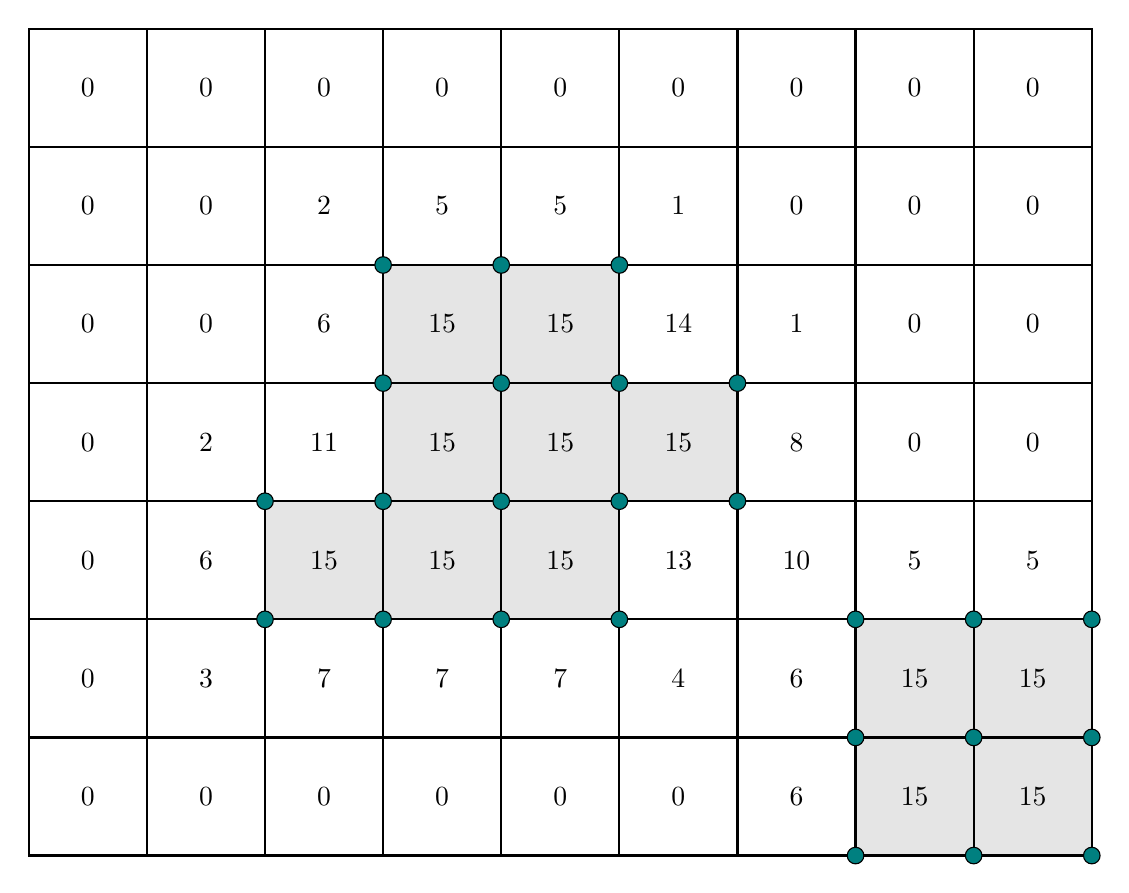
\begin{tikzpicture}
%\draw[step=0.5cm,gray,very thin] (0,0) grid (14,11); 

\draw[fill=gray!20](3,3) rectangle (7.5,4.5);  
\draw[fill=gray!20](4.5,4.5) rectangle (7.5,7.5);  
\draw[fill=gray!20](7.5,4.5) rectangle (9,6);  
\draw[fill=gray!20](10.5,0) rectangle (13.5,3);  

\draw[thick](0,0) rectangle (13.5,10.5);
\draw[thick](0,1.5)--(13.5,1.5);
\draw[thick](0,3)--(13.5,3);
\draw[thick](0,4.5)--(13.5,4.5);
\draw[thick](0,6)--(13.5,6);
\draw[thick](0,7.5)--(13.5,7.5);
\draw[thick](0,9)--(13.5,9);

\draw[thick](1.5,0)--(1.5,10.5);
\draw[thick](3,0)--(3,10.5);
\draw[thick](4.5,0)--(4.5,10.5);
\draw[thick](6,0)--(6,10.5);
\draw[thick](7.5,0)--(7.5,10.5);
\draw[thick](9,0)--(9,10.5);
\draw[thick](10.5,0)--(10.5,10.5);
\draw[thick](12,0)--(12,10.5);

\node[] at (0.75,0.75) {$0$};
\node[] at (2.25,0.75) {$0$};
\node[] at (3.75,0.75) {$0$};
\node[] at (5.25,0.75) {$0$};
\node[] at (6.75,0.75) {$0$};
\node[] at (8.25,0.75) {$0$};
\node[] at (9.75,0.75) {$6$};
\node[] at (11.25,0.75) {$15$};
\node[] at (12.75,0.75) {$15$};

\node[] at (0.75,2.25) {$0$};
\node[] at (2.25,2.25) {$3$};
\node[] at (3.75,2.25) {$7$};
\node[] at (5.25,2.25) {$7$};
\node[] at (6.75,2.25) {$7$};
\node[] at (8.25,2.25) {$4$};
\node[] at (9.75,2.25) {$6$};
\node[] at (11.25,2.25) {$15$};
\node[] at (12.75,2.25) {$15$};

\node[] at (0.75,3.75) {$0$};
\node[] at (2.25,3.75) {$6$};
\node[] at (3.75,3.75) {$15$};
\node[] at (5.25,3.75) {$15$};
\node[] at (6.75,3.75) {$15$};
\node[] at (8.25,3.75) {$13$};
\node[] at (9.75,3.75) {$10$};
\node[] at (11.25,3.75) {$5$};
\node[] at (12.75,3.75) {$5$};

\node[] at (0.75,5.25) {$0$};
\node[] at (2.25,5.25) {$2$};
\node[] at (3.75,5.25) {$11$};
\node[] at (5.25,5.25) {$15$};
\node[] at (6.75,5.25) {$15$};
\node[] at (8.25,5.25) {$15$};
\node[] at (9.75,5.25) {$8$};
\node[] at (11.25,5.25) {$0$};
\node[] at (12.75,5.25) {$0$};

\node[] at (0.75,6.75) {$0$};
\node[] at (2.25,6.75) {$0$};
\node[] at (3.75,6.75) {$6$};
\node[] at (5.25,6.75) {$15$};
\node[] at (6.75,6.75) {$15$};
\node[] at (8.25,6.75) {$14$};
\node[] at (9.75,6.75) {$1$};
\node[] at (11.25,6.75) {$0$};
\node[] at (12.75,6.75) {$0$};

\node[] at (0.75,8.25) {$0$};
\node[] at (2.25,8.25) {$0$};
\node[] at (3.75,8.25) {$2$};
\node[] at (5.25,8.25) {$5$};
\node[] at (6.75,8.25) {$5$};
\node[] at (8.25,8.25) {$1$};
\node[] at (9.75,8.25) {$0$};
\node[] at (11.25,8.25) {$0$};
\node[] at (12.75,8.25) {$0$};

\node[] at (0.75,9.75) {$0$};
\node[] at (2.25,9.75) {$0$};
\node[] at (3.75,9.75) {$0$};
\node[] at (5.25,9.75) {$0$};
\node[] at (6.75,9.75) {$0$};
\node[] at (8.25,9.75) {$0$};
\node[] at (9.75,9.75) {$0$};
\node[] at (11.25,9.75) {$0$};
\node[] at (12.75,9.75) {$0$};







\draw[black,fill=teal] (3,3) circle (3pt);
\draw[black,fill=teal] (4.5,3) circle (3pt);
\draw[black,fill=teal] (6,3) circle (3pt);
\draw[black,fill=teal] (7.5,3) circle (3pt);
\draw[black,fill=teal] (10.5,3) circle (3pt);
\draw[black,fill=teal] (12,3) circle (3pt);
\draw[black,fill=teal] (13.5,3) circle (3pt);
\draw[black,fill=teal] (10.5,1.5) circle (3pt);
\draw[black,fill=teal] (12,1.5) circle (3pt);
\draw[black,fill=teal] (13.5,1.5) circle (3pt);
\draw[black,fill=teal] (10.5,0) circle (3pt);
\draw[black,fill=teal] (12,0) circle (3pt);
\draw[black,fill=teal] (13.5,0) circle (3pt);
\draw[black,fill=teal] (3,4.5) circle (3pt);
\draw[black,fill=teal] (4.5,4.5) circle (3pt);
\draw[black,fill=teal] (6,4.5) circle (3pt);
\draw[black,fill=teal] (7.5,4.5) circle (3pt);
\draw[black,fill=teal] (9,4.5) circle (3pt);
\draw[black,fill=teal] (4.5,6) circle (3pt);
\draw[black,fill=teal] (6,6) circle (3pt);
\draw[black,fill=teal] (7.5,6) circle (3pt);
\draw[black,fill=teal] (9,6) circle (3pt);
\draw[black,fill=teal] (4.5,7.5) circle (3pt);
\draw[black,fill=teal] (6,7.5) circle (3pt);
\draw[black,fill=teal] (7.5,7.5) circle (3pt);


\end{tikzpicture}

\end{center}

The type is stored in the elemental array {\tt crtype} while the nodes belonging to elements 
to be refined are stored in {\tt crnode}.
There are 15 types of elements (the element type is tied to how many and which vertices are flagged nodes):

\begin{center}
\begin{flushright} {\tiny {\color{gray} (tikz\_cr\_2.tex)}} \end{flushright}
%~~~~~~~~~~~~~~~~~~~~~~~~~~~~~~~~~~~~~~~~~~~~~~~~~~~~~~~~~~~~~~~~~~~~~~~~~~~~~~~~~~~~~~~~~~~~~~~~~~

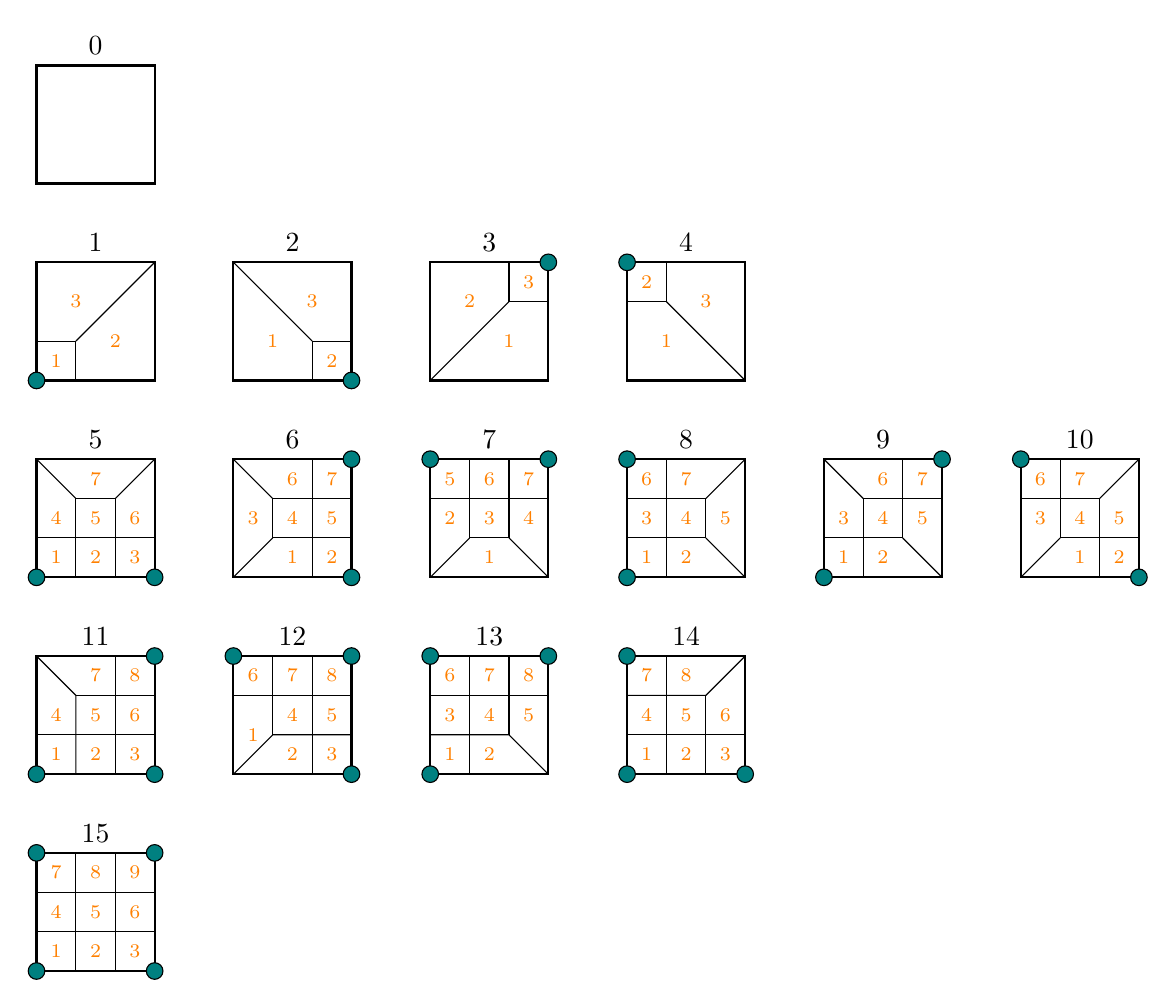
\begin{tikzpicture}
%\draw[step=1cm,gray,very thin] (0,0) grid (17,13); 

%.............................
\node[] at (1.25,12.25) {$0$};
\draw[thick](0.5,10.5) rectangle (2,12); %0

%.............................
\node[] at (1.25,9.75) {$1$};
\draw[thick](0.5,8) rectangle (2,9.5);   %1
\draw[black,fill=teal] (0.5,8) circle (3pt);
\draw[](1,8.5)--(2,9.5);   
\draw[](0.5,8.5)--(1,8.5)--(1,8);   

\node[] at (0.75,8.25) {\scriptsize \color{orange} 1};
\node[] at (1.5,8.5) {\scriptsize \color{orange} 2};
\node[] at (1,9) {\scriptsize \color{orange} 3};

%.............................
\node[] at (3.75,9.75) {$2$};
\draw[thick](3,8) rectangle (4.5,9.5); %2
\draw[black,fill=teal] (4.5,8) circle (3pt);
\draw[](4,8)--(4,8.5)--(4.5,8.5);
\draw[](3,9.5)--(4,8.5);
\node[] at (3.5,8.5) {\scriptsize \color{orange} 1};
\node[] at (4.25,8.25) {\scriptsize \color{orange} 2};
\node[] at (4,9) {\scriptsize \color{orange} 3};


%.............................
\node[] at (6.25,9.75) {$3$};
\draw[thick](5.5,8) rectangle (7,9.5); %3
\draw[black,fill=teal] (7,9.5) circle (3pt);
\draw[](5.5,8)--(6.5,9);
\draw[](6.5,9.5)--(6.5,9)--(7,9);
\node[] at (6.5,8.5) {\scriptsize \color{orange} 1};
\node[] at (6,9) {\scriptsize \color{orange} 2};
\node[] at (6.75,9.25) {\scriptsize \color{orange} 3};


%.............................
\node[] at (8.75,9.75) {$4$};
\draw[thick](8,8) rectangle (9.5,9.5); %4
\draw[black,fill=teal] (8,9.5) circle (3pt);
\draw[](8,9)--(8.5,9)--(8.5,9.5);
\draw[](8.5,9)--(9.5,8);
\node[] at (8.5,8.5) {\scriptsize \color{orange} 1};
\node[] at (8.25,9.25) {\scriptsize \color{orange} 2};
\node[] at (9,9) {\scriptsize \color{orange} 3};


%.............................
\node[] at (1.25,7.25) {$5$};
\draw[thick](0.5,5.5) rectangle (2,7);   %5
\draw[](0.5,6)--(2,6);
\draw[](1,5.5)--(1,6.5)--(1.5,6.5)--(1.5,5.5);
\draw[](0.5,7)--(1,6.5);
\draw[](2,7)--(1.5,6.5);
\draw[black,fill=teal] (0.5,5.5) circle (3pt);
\draw[black,fill=teal] (2,5.5) circle (3pt);

\node[] at (0.75,5.75) {\scriptsize \color{orange} 1};
\node[] at (1.25,5.75) {\scriptsize \color{orange} 2};
\node[] at (1.75,5.75) {\scriptsize \color{orange} 3};
\node[] at (0.75,6.25) {\scriptsize \color{orange} 4};
\node[] at (1.25,6.25) {\scriptsize \color{orange} 5};
\node[] at (1.75,6.25) {\scriptsize \color{orange} 6};
\node[] at (1.25,6.75) {\scriptsize \color{orange} 7};

%.............................
\node[] at (3.75,7.25) {$6$};
\draw[thick](3,5.5) rectangle (4.5,7);   %6
\draw[](4,5.5)--(4,7);
\draw[](4.5,6.5)--(3.5,6.5)--(3.5,6)--(4.5,6);
\draw[](3,5.5)--(3.5,6);
\draw[](3,7)--(3.5,6.5);
\draw[black,fill=teal] (4.5,5.5) circle (3pt);
\draw[black,fill=teal] (4.5,7) circle (3pt);

\node[] at (3.75,5.75) {\scriptsize \color{orange} 1};
\node[] at (4.25,5.75) {\scriptsize \color{orange} 2};
\node[] at (3.25,6.25) {\scriptsize \color{orange} 3};
\node[] at (3.75,6.25) {\scriptsize \color{orange} 4};
\node[] at (4.25,6.25) {\scriptsize \color{orange} 5};
\node[] at (3.75,6.75) {\scriptsize \color{orange} 6};
\node[] at (4.25,6.75) {\scriptsize \color{orange} 7};


%.............................
\node[] at (6.25,7.25) {$7$};
\draw[thick](5.5,5.5) rectangle (7,7);   %7
\draw[](5.5,6.5)--(7,6.5);
\draw[](6,7)--(6,6)--(6.5,6)--(6.5,7);
\draw[](5.5,5.5)--(6,6);
\draw[](7,5.5)--(6.5,6);
\draw[black,fill=teal] (5.5,7) circle (3pt);
\draw[black,fill=teal] (7,7) circle (3pt);


\node[] at (6.25,5.75) {\scriptsize \color{orange} 1};
\node[] at (5.75,6.25) {\scriptsize \color{orange} 2};
\node[] at (6.25,6.25) {\scriptsize \color{orange} 3};
\node[] at (6.75,6.25) {\scriptsize \color{orange} 4};
\node[] at (5.75,6.75) {\scriptsize \color{orange} 5};
\node[] at (6.25,6.75) {\scriptsize \color{orange} 6};
\node[] at (6.75,6.75) {\scriptsize \color{orange} 7};



%.............................
\node[] at (8.75,7.25) {$8$};
\draw[thick](8,5.5) rectangle (9.5,7);   %8
\draw[](8.5,5.5)--(8.5,7);
\draw[](8,6)--(9,6)--(9,6.5)--(8,6.5);
\draw[](9,6.5)--(9.5,7);
\draw[](9,6)--(9.5,5.5);
\draw[black,fill=teal] (8,5.5) circle (3pt);
\draw[black,fill=teal] (8,7) circle (3pt);

\node[] at (8.25,5.75) {\scriptsize \color{orange} 1};
\node[] at (8.75,5.75) {\scriptsize \color{orange} 2};
\node[] at (8.25,6.25) {\scriptsize \color{orange} 3};
\node[] at (8.75,6.25) {\scriptsize \color{orange} 4};
\node[] at (9.25,6.25) {\scriptsize \color{orange} 5};
\node[] at (8.25,6.75) {\scriptsize \color{orange} 6};
\node[] at (8.75,6.75) {\scriptsize \color{orange} 7};


%.............................
\node[] at (11.25,7.25) {$9$};
\draw[thick](10.5,5.5) rectangle (12,7);   %9

\draw[](10.5,7)--(11,6.5);
\draw[](11.5,6)--(12,5.5);
\draw[](11,6.5)--(11.5,6.5)--(11.5,6)--(11,6)--cycle;
\draw[](11.5,7)--(11.5,6.5)--(12,6.5);
\draw[](10.5,6)--(11,6)--(11,5.5);

\draw[black,fill=teal] (10.5,5.5) circle (3pt);
\draw[black,fill=teal] (12,7) circle (3pt);

\node[] at (10.75,5.75) {\scriptsize \color{orange} 1};
\node[] at (11.25,5.75) {\scriptsize \color{orange} 2};
\node[] at (10.75,6.25) {\scriptsize \color{orange} 3};
\node[] at (11.25,6.25) {\scriptsize \color{orange} 4};
\node[] at (11.75,6.25) {\scriptsize \color{orange} 5};
\node[] at (11.25,6.75) {\scriptsize \color{orange} 6};
\node[] at (11.75,6.75) {\scriptsize \color{orange} 7};



%.............................
\node[] at (13.75,7.25) {$10$};
\draw[thick](13,5.5) rectangle (14.5,7);   %10

\draw[](14,5.5)--(14,6)--(14.5,6);
\draw[](13,6.5)--(13.5,6.5)--(13.5,7);
\draw[](13.5,6.5)--(14,6.5)--(14,6)--(13.5,6)--cycle;
\draw[](13,5.5)--(13.5,6);
\draw[](14,6.5)--(14.5,7);

\draw[black,fill=teal] (14.5,5.5) circle (3pt);
\draw[black,fill=teal] (13,7) circle (3pt);

\node[] at (13.75,5.75) {\scriptsize \color{orange} 1};
\node[] at (14.25,5.75) {\scriptsize \color{orange} 2};
\node[] at (13.25,6.25) {\scriptsize \color{orange} 3};
\node[] at (13.75,6.25) {\scriptsize \color{orange} 4};
\node[] at (14.25,6.25) {\scriptsize \color{orange} 5};
\node[] at (13.25,6.75) {\scriptsize \color{orange} 6};
\node[] at (13.75,6.75) {\scriptsize \color{orange} 7};


%.............................
\node[] at (1.25,4.75) {$11$};
\draw[thick](0.5,3) rectangle (2,4.5);   %11
\draw[black,fill=teal] (0.5,3) circle (3pt);
\draw[black,fill=teal] (2,3) circle (3pt);
\draw[black,fill=teal] (2,4.5) circle (3pt);
\draw[](0.5,3.5)-- (2,3.5);
\draw[](1,4)-- (2,4);
\draw[](0.5,4.5)-- (1,4)--(1,3);
\draw[](1.5,3)-- (1.5,4.5);

\node[] at (0.75,3.25) {\scriptsize \color{orange} 1};
\node[] at (1.25,3.25) {\scriptsize \color{orange} 2};
\node[] at (1.75,3.25) {\scriptsize \color{orange} 3};
\node[] at (0.75,3.75) {\scriptsize \color{orange} 4};
\node[] at (1.25,3.75) {\scriptsize \color{orange} 5};
\node[] at (1.75,3.75) {\scriptsize \color{orange} 6};
\node[] at (1.25,4.25) {\scriptsize \color{orange} 7};
\node[] at (1.75,4.25) {\scriptsize \color{orange} 8};



%.............................
\node[] at (3.75,4.75) {$12$};
\draw[thick](3,3) rectangle (4.5,4.5);   %12
\draw[](3,3)-- (3.5,3.5)--(4.5,3.5);
\draw[](4,4.5)--(4,3);
\draw[](3,4)--(4.5,4);
\draw[](3.5,4.5)--(3.5,3.5);
\draw[black,fill=teal] (3,4.5) circle (3pt);
\draw[black,fill=teal] (4.5,3) circle (3pt);
\draw[black,fill=teal] (4.5,4.5) circle (3pt);

\node[] at (3.25,3.5)  {\scriptsize \color{orange} 1};
\node[] at (3.75,3.25) {\scriptsize \color{orange} 2};
\node[] at (4.25,3.25) {\scriptsize \color{orange} 3};
\node[] at (3.75,3.75) {\scriptsize \color{orange} 4};
\node[] at (4.25,3.75) {\scriptsize \color{orange} 5};
\node[] at (3.25,4.25) {\scriptsize \color{orange} 6};
\node[] at (3.75,4.25) {\scriptsize \color{orange} 7};
\node[] at (4.25,4.25) {\scriptsize \color{orange} 8};


%.............................
\node[] at (6.25,4.75) {$13$};
\draw[thick](5.5,3) rectangle (7,4.5);   %13

\draw[](5.5,4)--(7,4);
\draw[](5.5,3.5)--(6.5,3.5)--(7,3);
\draw[](6.5,4.5)--(6.5,3.5);
\draw[](6,4.5)--(6,3);

\draw[black,fill=teal] (5.5,3) circle (3pt);
\draw[black,fill=teal] (5.5,4.5) circle (3pt);
\draw[black,fill=teal] (7,4.5) circle (3pt);

\node[] at (5.75,3.25) {\scriptsize \color{orange} 1};
\node[] at (6.25,3.25) {\scriptsize \color{orange} 2};
\node[] at (5.75,3.75) {\scriptsize \color{orange} 3};
\node[] at (6.25,3.75) {\scriptsize \color{orange} 4};
\node[] at (6.75,3.75) {\scriptsize \color{orange} 5};
\node[] at (5.75,4.25) {\scriptsize \color{orange} 6};
\node[] at (6.25,4.25) {\scriptsize \color{orange} 7};
\node[] at (6.75,4.25) {\scriptsize \color{orange} 8};



%.............................
\node[] at (8.75,4.75) {$14$};
\draw[thick](8,3) rectangle (9.5,4.5);   %14
\draw[black,fill=teal] (8,4.5) circle (3pt);
\draw[black,fill=teal] (8,3) circle (3pt);
\draw[black,fill=teal] (9.5,3) circle (3pt);
\draw[](8,3.5) -- (9.5,3.5);
\draw[](8,4) -- (9,4)--(9.5,4.5);
\draw[](9,3) -- (9,4);
\draw[](8.5,3) -- (8.5,4.5);

\node[] at (8.25,3.25) {\scriptsize \color{orange} 1};
\node[] at (8.75,3.25) {\scriptsize \color{orange} 2};
\node[] at (9.25,3.25) {\scriptsize \color{orange} 3};
\node[] at (8.25,3.75) {\scriptsize \color{orange} 4};
\node[] at (8.75,3.75) {\scriptsize \color{orange} 5};
\node[] at (9.25,3.75) {\scriptsize \color{orange} 6};
\node[] at (8.25,4.25) {\scriptsize \color{orange} 7};
\node[] at (8.75,4.25) {\scriptsize \color{orange} 8};

%.............................
\node[] at (1.25,2.25) {$15$};
\draw[thick](0.5,0.5) rectangle (2,2);   %15
\draw[black,fill=teal] (0.5,0.5) circle (3pt);
\draw[black,fill=teal] (2,0.5) circle (3pt);
\draw[black,fill=teal] (2,2) circle (3pt);
\draw[black,fill=teal] (0.5,2) circle (3pt);
\draw[](0.5,1) -- (2,1);  
\draw[](0.5,1.5) -- (2,1.5);  
\draw[](1,0.5) -- (1,2);  
\draw[](1.5,0.5) -- (1.5,2);  

\node[] at (0.75,0.75) {\scriptsize \color{orange} 1};
\node[] at (1.25,0.75) {\scriptsize \color{orange} 2};
\node[] at (1.75,0.75) {\scriptsize \color{orange} 3};
\node[] at (0.75,1.25) {\scriptsize \color{orange} 4};
\node[] at (1.25,1.25) {\scriptsize \color{orange} 5};
\node[] at (1.75,1.25) {\scriptsize \color{orange} 6};
\node[] at (0.75,1.75) {\scriptsize \color{orange} 7};
\node[] at (1.25,1.75) {\scriptsize \color{orange} 8};
\node[] at (1.75,1.75) {\scriptsize \color{orange} 9};

\end{tikzpicture}




\end{center}

Note that the refinement above is based on a 3x3 refinement of elements. One could also carry out a 5x5-type
refinement which would then rely on the following elements (and their rotated versions)\footnote{I have never
seen a concrete example of these...}:
\begin{center}
\begin{flushright} {\tiny {\color{gray} (tikz\_cr\_3.tex)}} \end{flushright}
%~~~~~~~~~~~~~~~~~~~~~~~~~~~~~~~~~~~~~~~~~~~~~~~~~~~~~~~~~~~~~~~~~~~~~~~~~~~~~~~~~~~~~~~~~~~~~~~~~~


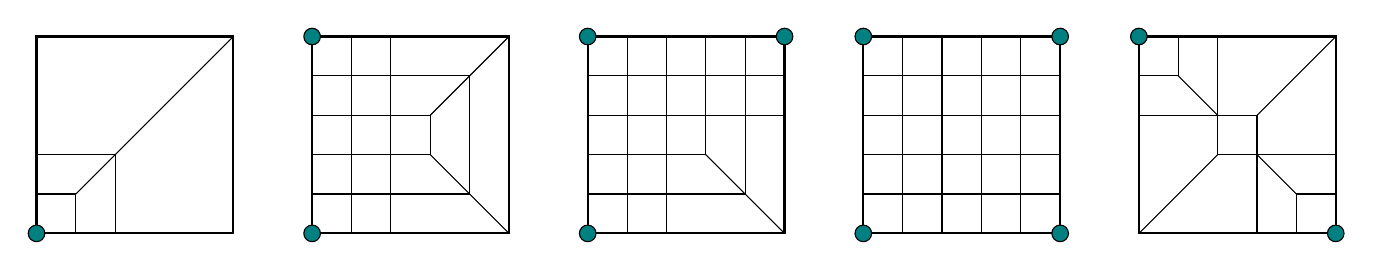
\begin{tikzpicture}
%\draw[step=0.5cm,gray,very thin] (0,0) grid (17,5); %background grid


\draw[thick] (0.5,0.5) rectangle (3,3);
\draw[](0.5,1)--(1,1)--(1,0.5);
\draw[](0.5,1.5)--(1.5,1.5)--(1.5,0.5);
\draw[](1,1)--(3,3);
\draw[black,fill=teal] (0.5,0.5) circle (3pt);


\draw[thick] (4,0.5) rectangle (6.5,3);
\draw[](4.5,0.5)--(4.5,3);
\draw[](5,0.5)--(5,3);
\draw[](4,1.5)--(5.5,1.5)--(5.5,2)--(4,2);
\draw[](4,1)--(6,1)--(6,2.5)--(4,2.5);
\draw[](5.5,2)--(6.5,3);
\draw[](5.5,1.5)--(6.5,0.5);
\draw[black,fill=teal] (4,0.5) circle (3pt);
\draw[black,fill=teal] (4,3) circle (3pt);

\draw[thick] (7.5,0.5) rectangle (10,3);
\draw[](8,0.5)--(8,3);
\draw[](8.5,0.5)--(8.5,3);
\draw[](7.5,2.5)--(10,2.5);
\draw[](7.5,2)--(10,2);
\draw[](7.5,1.5)--(9,1.5)--(9,3);
\draw[](7.5,1)--(9.5,1)--(9.5,3);
\draw[](9,1.5)--(10,0.5);
\draw[black,fill=teal] (7.5,0.5) circle (3pt);
\draw[black,fill=teal] (7.5,3) circle (3pt);
\draw[black,fill=teal] (10,3) circle (3pt);

\draw[thick] (11,0.5) rectangle (13.5,3);
\draw[](11,1)--(13.5,1);
\draw[](11,1.5)--(13.5,1.5);
\draw[](11,2)--(13.5,2);
\draw[](11,2.5)--(13.5,2.5);
\draw[](11.5,0.5)--(11.5,3);
\draw[](12,0.5)--(12,3);
\draw[](12.5,0.5)--(12.5,3);
\draw[](13,0.5)--(13,3);
\draw[black,fill=teal] (11,0.5) circle (3pt);
\draw[black,fill=teal] (11,3) circle (3pt);
\draw[black,fill=teal] (13.5,3) circle (3pt);
\draw[black,fill=teal] (13.5,0.5) circle (3pt);

\draw[thick] (14.5,0.5) rectangle (17,3);
\draw[black,fill=teal] (14.5,3) circle (3pt);
\draw[black,fill=teal] (17,0.5) circle (3pt);
\draw[](14.5,0.5)--(15.5,1.5);
\draw[](16,2)--(17,3);
\draw[](15.5,1.5) rectangle (16,2);
\draw[](14.5,2.5)--(15,2.5)--(15,3);
\draw[](14.5,2)--(15.5,2)--(15.5,3);
\draw[](15,2.5)--(15.5,2);
\draw[](16,1.5)--(16.5,1);
\draw[](16.5,0.5)--(16.5,1)--(17,1);
\draw[](16,0.5)--(16,1.5)--(17,1.5);

\end{tikzpicture}



\end{center}

After running the code, various vtu files are to be found in the OUT folder.
{\filenamefont solution.vtu} contains the refined mesh with the calculated 
solution. 

\newpage
%................................................................
\paragraph{Case test=0}

The domain size is 9x7 and nelx=9, nely=7, so that all elements are square. 
The code solves the FE system but it is pointless as this test is about demonstrating 
the resulting mesh from the flagged elements at the beginning of this stone. 

\begin{center}
a)\includegraphics[width=7cm]{python_codes/fieldstone_102/results/test0/mesh1}
b)\includegraphics[width=7cm]{python_codes/fieldstone_102/results/test0/mesh2}\\
c)\includegraphics[width=7cm]{python_codes/fieldstone_102/results/test0/mesh3}
d)\includegraphics[width=7cm]{python_codes/fieldstone_102/results/test0/mesh4}\\
{\captionfont a) original mesh. b) flagged nodes. c) element types. d) refined mesh.}
\end{center}

%................................................................
\paragraph{Case test=1,2,3}

\begin{center}
\includegraphics[width=5.6cm]{python_codes/fieldstone_102/results/test1/vel}
\includegraphics[width=5.6cm]{python_codes/fieldstone_102/results/test2/vel}
\includegraphics[width=5.6cm]{python_codes/fieldstone_102/results/test3/vel}\\
\includegraphics[width=5.6cm]{python_codes/fieldstone_102/results/test1/press}
\includegraphics[width=5.6cm]{python_codes/fieldstone_102/results/test2/press}
\includegraphics[width=5.6cm]{python_codes/fieldstone_102/results/test3/press}\\
{\captionfont Initial resolution 10x10. 
Left: The left half of elements are flagged for refinement.
Middle: The elements above the diagonal are flagged for refinement.
Right: Every 7 elements is flagged for refinement.}
\end{center}

















 %%%%%%%%%%%%%%%%%%%%%%%%%%%%%%%%%%%%%%%%%%%%%%%%%

\newpage %%%%%%%%%%%%%%%%%%%%%%%%%%%%%%%%%%%%%%%%%%%%%%%%%%%%%%%%%%%%%%%%%%%%%%%%%%%%%%%%
\section*{
Stone 103: conformal mesh refinement in 3D 
\label{f103}}
\addcontentsline{toc}{section}{\protect\numberline{} 
Stone 103: conformal mesh refinement in 3D 
}
\lstinputlisting[language=bash,basicstyle=\small]{python_codes/fieldstone_103/keywords}

\begin{center}
Code at \url{https://github.com/cedrict/fieldstone/tree/master/python_codes/fieldstone_103}
\end{center}

\par\noindent\rule{\textwidth}{0.4pt}

%%%%%%%%%%%%%%%%%%%%%%%%%%%%%%%%%%%%%%%%%%%%%%%%%%%%%%%%%%%%%%%%%%%%%%%%%%%%%%%%%%%%%%%%%%%%%%%%%%%%

\begin{center}
\includegraphics[width=1cm]{images/fortran/fortran} 
\end{center}

The topic of Conformal Mesh Refinement is introduced in Section~\ref{ss:cmr}.
This code is in Fortran for the same reason \stone~102 is. 
However, it is not nearly as complete as \stone~102: It can only refine 
above a certain height, as the different types of subdivisions are not implemented.
Furthermore, there is no FE solver in it either. It is just an example of 
simple 3D conformal refinement meshing.

The {\filenamefont prog.f90} code showcases the decomposition of one element and generates
the {\filenamefont refined.vtu} file:
\begin{center}
\includegraphics[width=4.5cm]{python_codes/fieldstone_103/visu1}
\includegraphics[width=4.5cm]{python_codes/fieldstone_103/visu2}
\includegraphics[width=4.5cm]{python_codes/fieldstone_103/visu3}
\end{center}
The internal numbering goes as follows:
\begin{center}
\includegraphics[width=7cm]{python_codes/fieldstone_103/images/numbering}\\
{\captionfont Taken from ? Numbers added by me. There are additional handwritten notes
in the images folder.}
\end{center}

In order to finish the {\filenamefont stone.f90} code, one would need to 
implement all four (+rotations) of these subdivisions:
\begin{center}
\includegraphics[width=8cm]{python_codes/fieldstone_103/images/scde}\\
{\captionfont Taken from ?}
\end{center}

Note that there is another way to subdivide an element:
\begin{center}
\includegraphics[width=5cm]{python_codes/fieldstone_103/images/habo04}\\
{\captionfont Taken from \cite{habo04}.}
\end{center}

Finally, we can run the code on a $20\times16\times12$ original mesh:
\begin{center}
\includegraphics[width=7cm]{python_codes/fieldstone_103/before}
\includegraphics[width=7cm]{python_codes/fieldstone_103/after}
\end{center}

 %%%%%%%%%%%%%%%%%%%%%%%%%%%%%%%%%%%%%%%%%%%%%%%%%

\newpage %%%%%%%%%%%%%%%%%%%%%%%%%%%%%%%%%%%%%%%%%%%%%%%%%%%%%%%%%%%%%%%%%%%%%%%%%%%%%%%%
\section*{
Stone 104: grad-div stabilisation 
\label{f104}}
\addcontentsline{toc}{section}{\protect\numberline{} 
Stone 104: grad-div stabilisation 
}

Note to self: normalisation does not work for Q2Q1.

All the following benchmarks are isoviscous with $\eta=1$ and are valid in the unit square domain. 
As such the scaling coefficient between blocks $\K$ and $\G$ of the Stokes matrix (see Section~\ref{XYZ}) 
is 1 and won't play any role in the results. 

REDO all with aspect

According to Jenkins \etal (2014) \cite{jejl14}, Grad-div stabilization results from adding
$\vec{0} = - \gamma \vec\nabla (\vec\nabla\cdot \vec\upnu)$ to the continuous Stokes
equations, i.e.:
\[
-\nabla p  + \nabla \cdot ( 2 \eta \dot{\bm \varepsilon}) + \rho \vec{g} 
= - \gamma \vec\nabla (\vec\nabla\cdot \vec\upnu)
\]
We immediately notice that the aditional term is in fact identical to the penalty term and 
its weak form and discretisation is worked out in Section~\ref{XXX}, so that 
the matrix $\K$ then becomes:
\[
\K = \int {\bm B}^T \cdot [ \gamma {\bm K} + \eta {\bm C} ] \cdot {\bm B} \; dV
\]
with 
\[
{\bm C}=
\left(
\begin{array}{ccc}
2 & 0 & 0 \\
0 & 2 & 0 \\
0 & 0 & 1 
\end{array}
\right)
\qquad
{\bm K}=
\left(
\begin{array}{ccc}
1 & 1 & 0 \\
1 & 1 & 0 \\
0 & 0 & 0 
\end{array}
\right)
\]
The implementation is then trivial. Surprisingly in the papers on the grad-div stabilisation 
the penalty method is never mentioned (?) although John \etal state that 
"[...] it shall be emphasized that large
contributions of the grad-div stabilization result in linear systems of equations with
large condition numbers", which is a well know problem of the penalty method.

In this case $\gamma>0$ but another parallel can be drawn when $\gamma = -\frac{2}{3}\eta$. In that case
\[
 \nabla \cdot ( 2 \eta \dot{\bm \varepsilon}) + \gamma \vec\nabla (\vec\nabla\cdot \vec\upnu)
=
 \nabla \cdot ( 2 \eta \dot{\bm \varepsilon}) -\frac{2\eta}{3} \vec\nabla (\vec\nabla\cdot \vec\upnu)
=
 \nabla \cdot 2 \eta ( \dot{\bm \varepsilon} -\frac{1}{3} (\vec\nabla\cdot \vec\upnu) {\bm 1} )
= 
 \nabla \cdot 2 \eta \dot{\bm \varepsilon}^d 
\]
Obviously $\gamma$ should not be `too negative', otherwise terms on the diagonal 
of $\gamma {\bm K} + \eta {\bm C} $
will be negative and this will cause problems. 

In what follows I have implemented what I think the grad-div method is, with 
rather limited/puzzling (?) results.
Rather importantly John \etal conclude that ``the
grad-div stabilization might improve the pressure-robustness in certain situations but
it is not a remedy''. 

\Literature: \cite{ollh09}

%---------------------------------------------------------------------
\subsubsection*{Experiment=1: Donea \& Huerta manufactured solution}

I carry out this benchmark to make sure that the code behaves as expected and that the
error rates are what we expect: 3rd order for velocity, second order for pressure 
for both $Q_2\times Q_1$ and $Q_2\times P_{-1}$ elements (see for instance 
Thieulot \& Bangerth \cite{thba21}).

\begin{center}
\includegraphics[width=8cm]{python_codes/fieldstone_104/results/exp1/errors.pdf}
\end{center}


%---------------------------------------------------------------------
\subsubsection*{Experiment=2: example 1.1 in John \etal (2017)}
Following John \etal (2017) \cite{jolm17} we 
postulate the following velocity and pressure fields:
\begin{eqnarray}
\vec{\upnu}(x,y) &=& \vec{0} \nn\\
p(x,y) &=& \Ranb ( y^3-y^2/2+y-7/12 ) \nn
\end{eqnarray}
with $\eta=1$ and the buoyancy force vector is
\[
\vec{b}=
\left(
\begin{array}{c}
0 \\ \Ranb(1-y+3y^2)
\end{array}
\right)
\]

\begin{center}
\includegraphics[height=4cm]{python_codes/fieldstone_104/results/exp2/errors.pdf}
\includegraphics[height=4cm]{python_codes/fieldstone_104/results/exp2/jolm17a}\\
{\captionfont Left: this stone; Right: taken from \cite{jolm17}}
\end{center}

We find that the velocity error magnitude for the $Q_2\times Q_1$ element
scales with the Rayleigh number, and 
more surprisingly (?) that its convergence is quartic.
However, the velocity error magnitude for the $Q_2\times P_{-1}$ 
remains very low independently of the Rayleigh number

\begin{center}
\includegraphics[height=6cm]{python_codes/fieldstone_104/results/exp2/gamma/errors.pdf}
\end{center}

%---------------------------------------------------------------------
\subsubsection*{Experiment=3,4,5: }

These three manufactured solutions come from Jenkins \etal (2014) \cite{jejl14}.
The velocity is the same in all cases, $\vec{\upnu}=(\cos 2\pi y , \sin 2\pi x)$
while the three pressure fields are
\begin{eqnarray}
p_1(x,y) &=& \sin (2\pi y)  \nn\\
p_2(x,y) &=& \sin (8 \pi y)   \nn\\
p_3(x,y) &=& 10^4 \sin (2\pi y) \nn
\end{eqnarray}
We need to compute the vector $\vec{b}$ from these. 
The strain rate tensor is then 
\[
\dot{\bm \varepsilon}(\vec{\upnu}) = 
\left(
\begin{array}{cc}
0 &  - \pi \sin 2\pi y + \pi \cos 2 \pi x  \\
 - \pi \sin 2\pi y + \pi \cos 2 \pi x   & 0
\end{array}
\right)
\]
and then the full stress tensor:
\[
{\bm \sigma} = 
- p {\bm 1}+ 2 \eta \dot{\bm \varepsilon}
= \left(
\begin{array}{cc}
-p &  -2 \pi \eta (\sin 2\pi y -  \cos 2 \pi x)  \\
-2 \pi \eta (\sin 2\pi y -  \cos 2 \pi x)   & -p
\end{array}
\right)
\]
Finally
\[
-\vec{b} = 
\vec\nabla \cdot {\bm \sigma} = 
\left(
\begin{array}{c}
-\partial_x p - 4 \pi^2 \eta \cos 2\pi y  \\ 
-\partial_y p - 4 \pi^2 \eta \sin 2\pi x 
\end{array}
\right)
\]
We see that we have $\partial_x p_{1,2,3} =0$ so 
\[
\vec{b}
=
\left(
\begin{array}{c}
 4 \pi^2 \eta \cos 2\pi y  \\ 
\partial_y p + 4 \pi^2 \eta \sin 2\pi x 
\end{array}
\right)
\]

\begin{center}
\includegraphics[width=5cm]{python_codes/fieldstone_104/results/exp3/errors.pdf}
\includegraphics[width=5cm]{python_codes/fieldstone_104/results/exp4/errors.pdf}
\includegraphics[width=5cm]{python_codes/fieldstone_104/results/exp5/errors.pdf}
\end{center}

We see that the Q2Q1 velocity error is much larger than the Q2P1 error in benchmark 3 
but that it converges again in a quartic manner.
Pressure errors are however identical.

%------------------------------------------------------------------------------------------
\subsubsection*{Experiment=6: manufactured solution in John \etal (2017) \cite{jolm17}}

See Section~\ref{ss:mmsjolm17} for details.

\begin{center}
\includegraphics[width=5cm]{python_codes/fieldstone_104/results/exp6/vel}
\includegraphics[width=5cm]{python_codes/fieldstone_104/results/exp6/press}
\includegraphics[width=5cm]{python_codes/fieldstone_104/results/exp6/errors.pdf}
\end{center}


\begin{center}
\includegraphics[height=6cm]{python_codes/fieldstone_104/results/exp6/gamma/errors.pdf}\\
{\captionfont errors as a function of $\gamma$.}
\end{center}



 %%%%%%%%%%%%%%%%%%%%%%%%%%%%%%%%%%%%%%%%%%%%%%%%%

\newpage %%%%%%%%%%%%%%%%%%%%%%%%%%%%%%%%%%%%%%%%%%%%%%%%%%%%%%%%%%%%%%%%%%%%%%%%%%%%%%%%
\section*{
Stone 105: solving the flexure equation with FDM 
\label{f105}}
\addcontentsline{toc}{section}{\protect\numberline{} 
Stone 105: solving the flexure equation with FDM 
}
\lstinputlisting[language=bash,basicstyle=\small]{python_codes/fieldstone_105/keywords}

\begin{center}
Code at \url{https://github.com/cedrict/fieldstone/tree/master/python_codes/fieldstone_105}
\end{center}

\par\noindent\rule{\textwidth}{0.4pt}

{\sl This stone was developed in collaboration with Zolt{\'a}n Erd{\H{o}}s}. 
\index{contributors}{Z. Erd{\H{o}}s}

\par\noindent\rule{\textwidth}{0.4pt}

%%%%%%%%%%%%%%%%%%%%%%%%%%%%%%%%%%%%%%%%%%%%%%%%%%%%%%%%%%%%%%%%%%%%%%%%%%%%%%%%%%%%%%%%%%%%%%%%%%%%

Under many simplifying approximations (See Section ~3.9 of Turcotte \& Schubert book), the simplest time-independent flexure equation is
\[
D \frac{d^4w(x)}{dx^4} + P \frac{d^2w(x)}{dx^2} + (\rho_m-\rho_c)g w(x) = q(x)
\]
where $w(x)$ is the plate deflection (\si{m}), 
\[
D=\frac{E t^3}{12(1-\nu^2)}
\]
is the flexural rigidity, with $t$ the thickness of the plate (\si{m}), $E$ is Young's modulus, $\nu$ is the Poisson ratio, $P$ is a horizontal force per unit length (\si{\kg\per\square\metre\square\sec}),  $q$ is the load (\si{\pascal}), $\rho_m$ is the mantle density and $\rho_c$ is the density of the crust (\si{\kg\per\cubic\metre}).
This is a 4th-order ODE. In order to solve it, we will need 4 boundary conditions.

Redo Fig. 3.24 of T\&S. 

We wish to solve this equation on the domain $[0,L_x]$ with the Finite Difference method. Indeed the presence of a 4th-order derivative poses quite a few problems for the Finite Element method and in this case the FDM is more straighforward to implement. The domain is discretised with $n_p$ nodes equally spaced by $h=L_x/(n_p-1)$.

We will need the 2nd- and 4th-order derivatives\footnote{\url{https://en.wikipedia.org/wiki/Finite_difference_coefficient}}:
\begin{eqnarray}
\frac{d^2w}{dx^2} &=& \frac{w_{n-1}-2w_n+w_{n+1}}{h^2} 
+{\cal O}(h^3) \\
\frac{d^4w}{dx^4} &=& \frac{w_{n-2}-4w_{n-1}+6w_n-4w_{n+1}+w_{n+1}}{h^4}
+{\cal O}(h^5)
\end{eqnarray}
Both are second-order accurate.
We then obtain 
\[
D\frac{w_{n-2}-4w_{n-1}+6w_n-4w_{n+1}+w_{n+1}}{h^4}
+P\frac{w_{n-1}-2w_n+w_{n+1}}{h^2} 
+(\rho_m-\rho_c)g w_n = q_n
\]
or, 
\[
\boxed{
\frac{D}{h^4} w_{n-2}
+\left(-\frac{4D}{h^4}+\frac{P}{h^2}\right)w_{n-1}
+\left(\frac{6D}{h^4}-\frac{2P}{h^2} +(\rho_m-\rho_c)g \right)w_n
+\left(-\frac{4D}{h^4}+\frac{P}{h^2}\right)w_{n+1}
+\frac{D}{h^4} w_{n+2} = q_n
}
\]
One could also multiply this equation by $h^4$ and obtain:
\[
D w_{n-2}
+\left(-4D+Ph^2\right)w_{n-1}
+\left(6D-2Ph^2 +(\rho_m-\rho_c)g h^4 \right)w_n
+\left(-4D+Ph^2\right)w_{n+1}
+D w_{n+2} = q_n h^4
\]
We will formulate this equation for every node $i\in[2,n_p-3]$
in a systematic manner and we will therefore obtain a linear system of equations of the form 
\[
{\bm A} \cdot \vec{w} = \vec{b}
\]
where ${\bm A}$ is an $n_p\times n_p$ matrix (sparse since pentadiagonal) and $\vec{b}$ the right-hand side vector. 
The vector $\vec{w}$ contains the $n_p$ deflection unknowns at the nodes of the mesh.

\begin{center}
\includegraphics[width=4cm]{python_codes/fieldstone_105/images/matrix}
\end{center}

The four missing lines are addressed when we consider the boundary conditions:
We assume the plate to be very long, and that the load(s) will be mostly concentrated around $L_x/2$ . We therefore 
prescribe $w=0$ and $dw/dx=0$ at $x=0$ and $x=L_x$ (i.e. the deflection and the slope at the edges of the beam both tend to zero).

The first condition is trivial to impose: set 1 on the diagonal of the matrix for $i=0$ and $i=n_p-1$ and the corresponding entries of the rhs to zero. 
The second will have us use the backward derivative on the left for node $i=1$ and the forward derivative on the right for node $n_p-2$:
\begin{eqnarray}
\frac{dw}{dx} (x=0)   &\simeq& \frac{-w_0+w_1}{h} \nonumber\\
\frac{dw}{dx} (x=L_x) &\simeq& \frac{-w_{n_p-2}+w_{n_p-1}}{h}
\end{eqnarray}
The two equations will replace the second and before last 
lines in the matrix.

The flexure equation which allows for $D$ to be a function of space is 
\[
\frac{d^2}{dx^2} \left( D(x) \frac{d^2w(x)}{dx^2} \right) + P \frac{d^2w(x)}{dx^2} + (\rho_m-\rho_c)g w(x) = q(x)
\]
Instead of using the expression for a 4th-order derivative we then use the expression for a 2nd-order derivative twice. 
Let us temporarily coin $\phi=D(x) \frac{d^2w}{dx^2}$.
Then
\begin{eqnarray}
&&\frac{d^2}{dx^2} \left( D(x) \frac{d^2w(x)}{dx^2} \right)\\
&=& \frac{d^2 \phi}{dx^2} \\
&\simeq& \frac{\phi_{n-1}-2\phi_n+\phi_{n+1}}{h^2} \nonumber\\
&\simeq& \frac{1}{h^2}
\left(
D_{n-1} \frac{w_{n-2}-2w_{n-1}+w_{n}}{h^2}
-2 D_n \frac{w_{n-1}-2w_n+w_{n+1}}{h^2}
+ D_{n+1} \frac{w_{n}-2w_{n+1}+w_{n+2}}{h^2}
\right) \nonumber\\
&=&
\frac{D_{n-1}}{h^4} w_{n-2}
-2\frac{D_{n-1}+D_n}{h^4} w_{n-1}
+\frac{D_{n-1}+4D_n+D_{n+1}  }{h^4} w_n
-2\frac{D_{n}+D_{n+1}}{h^4} w_{n+1}
+\frac{D_{n+1}}{h^4} w_{n+2} \nonumber
\end{eqnarray}
Obviously if $D_{n-1}=D_n=D_{n+1}$ we recover the 
expression above derived with a constant flexural 
rigidity $D$.
The full flexural equation with the variable $D(x)$ then reads as
\begin{eqnarray}
\frac{D_{n-1}}{h^4} w_{n-2}
+\left(-2\frac{D_{n-1}+D_{n}}{h^4}+\frac{P}{h^2}\right)w_{n-1}
+\left(\frac{D_{n-1}+4D_{n}+D_{n+1}}{h^4}-\frac{2P}{h^2} +(\rho_m-\rho_c)g \right)w_n \nonumber\\
+\left(-2\frac{D_{n}+D_{n+1}}{h^4}+\frac{P}{h^2}\right)w_{n+1}
+\frac{D_{n+1}}{h^4} w_{n+2} = q_n
\end{eqnarray}




%-------------------------------------------------
\subsubsection*{Benchmark 1: line load}

Following Buiter (2000) \cite{buiter_thesis} we consider the case of a lineload.
The lineload $F$ is applied in the middle of the domain and the solution 
is therefore symmetric around $x=L_x/2$.
The analytical solution is given by\footnote{I believe the absolute values
are missing in the thesis.} 
\[
w_{analytical} = \frac{F \alpha^3}{8 D} \exp -\frac{|x|}{\alpha}
\left(
\cos \frac{|x|}{\alpha} + \sin \frac{|x|}{\alpha} 
\right)
\]
with the so-called flexural parameter $\alpha$:
\[
\alpha=\left(\frac{4D}{(\rho_m-\rho_c)g}\right)^{1/4}
\]
measures the wavelength of the flexure.

\begin{center}
\includegraphics[width=5cm]{python_codes/fieldstone_105/images/buiter}
\includegraphics[width=8cm]{python_codes/fieldstone_105/results/bench1/w.pdf}\\
{\captionfont Left: Taken from \cite{buiter_thesis}}
\end{center}


%-------------------------------------------------
\subsubsection*{Benchmark 2: periodic loading}

For this benchmark we only prescribe $w=0$ at both extremities.

\[
q(x)=\rho_c g h_0 \sin 2\pi \frac{x}{\lambda}
\]

The solution is $w(x)=w_0 \sin 2\pi x/\lambda$, with 
\[
w_0=\frac{h_0}{\frac{\rho_m}{\rho_c}-1+\frac{D}{\rho_c g} (2\pi/\lambda)^4}
\]

\begin{center}
\includegraphics[width=8cm]{python_codes/fieldstone_105/results/bench2/w.pdf}\\
{\captionfont Obtained with $\lambda=0.5Lx$}
\end{center}


%-------------------------------------------------
\subsubsection*{Experiment 3: island}

The load is given by $q(x)=\rho_c g h_0 \left(1+\cos 2\pi \frac{|x-L_x/2|}{\lambda}\right) $
for $|x-L_x/2|<\lambda/2$ 

\begin{center}
\includegraphics[width=8cm]{python_codes/fieldstone_105/results/exp3/load}
\includegraphics[width=8cm]{python_codes/fieldstone_105/results/exp3/w.pdf}\\
{\captionfont Obtained with $\lambda=0.1$}
\end{center}



 %%%%%%%%%%%%%%%%%%%%%%%%%%%%%%%%%%%%%%%%%%%%%%%%%

\newpage %%%%%%%%%%%%%%%%%%%%%%%%%%%%%%%%%%%%%%%%%%%%%%%%%%%%%%%%%%%%%%%%%%%%%%%%%%%%%%%%
\section*{
Stone 106: plumes in axisymmetric chunk ($Q_2\times Q_1$) 
\label{f106}}
\addcontentsline{toc}{section}{\protect\numberline{} 
Stone 106: plumes in axisymmetric chunk ($Q_2\times Q_1$) 
}
\lstinputlisting[language=bash,basicstyle=\small]{python_codes/fieldstone_106/keywords}

\begin{center}
Code at \url{https://github.com/cedrict/fieldstone/tree/master/python_codes/fieldstone_106}
\end{center}

\par\noindent\rule{\textwidth}{0.4pt}

\Literature Kiefer \& Hager \cite{kiha92}, King \cite{king97}, Redmond \& King \cite{reki04},
Kiefer (2003) \cite{kief03}, Li \& Kiefer (2007) \cite{liki07}

\par\noindent\rule{\textwidth}{0.4pt}
%%%%%%%%%%%%%%%%%%%%%%%%%%%%%%%%%%%%%%%%%%%%%%%%%%%%%%%%%%%%%%%%%%%%%%%%%%%%%%%%%%%%%%%%%%%%%%%%%%%%

This stone is inspired by Kellogg \& King (1997) \cite{keki97}. 

\begin{center}
\includegraphics[width=6cm]{python_codes/fieldstone_106/images/keki97a}\\
{\captionfont Taken from \cite{keki97}.}
\end{center}

I set out to reproduce the results of the original publication. 
The necessary information is spread out throughout the first pages.
In Section~3 it is stated that the angular opening is $\pi/4$ and $r_i/r_o=0.55$.
However, it is not clear what $r_i$ or $r_o$ are, although Section~3
mentions $r$ values of 1.7 which is somewhat in the 'middle' of the cone. 
Because the equations in the paper are in dimensionless form, and 
because it is common to choose the depth of the mantle as reference length, 
then we probably have $r_o-r_i=1$. In this case we find $r_i=1.22\dots$ and 
$r_o=2.22\dots$ ({\color{orange} 1st guess}: confirmed by author S.K., June 2021. 
Also consistent with King \cite{king97}).

Free-slip boundary conditions are imposed on all boundaries.
A patch on the inner boundary of the shell is heated by
maintaining it at a constant dimensionless temperature of $T_{patch}=1$; 
elsewhere the base of the shell is insulating ($\partial T/\partial r = 0$).
At the top of the shell, a constant dimensionless temperature of $T_{top}=0$ was maintained.
Unfortunately it is not specified how wide the patch is, so I choose 
$\pi/8$ which seems probable when looking at 
Figure~3 of the paper ({\color{orange} 2nd guess}: confirmed by S.K., June 2021).
The sides of the cone are insulating ($\partial T/\partial \theta =0$).
Because of how FE works the insulating boundary conditions are automatically enforced 
when Dirichlet boundary conditions are absent. 

The viscous rheology is temperature-dependent:
\[
\eta(T) =\eta_0 \exp\left[ E \left( \frac{1}{T+T_0} -\frac{1}{1+T_0}  \right)   \right]
\]
with $E= \{0,0.25328,3\}$. $T_0$ is defined as ``the surface temperature divided by the temperature
drop across the shell'' but its value is not specified. On Earth the surface temperature 
is $\sim300\si{\kelvin}$
while the temperature drop across the mantle is $\sim3000\si{\kelvin}$ 
so I take $T_0=0.1$ ({\color{orange} 3rd guess}: S.K. says that $\Delta T$ can be recovered from 
the Rayleigh number and using standard Earth values for all other parameters, but given the uncertainty about 
the Rayleigh number itself, this parameter is lost forever).
The value for $\eta_0$ is also not specified but if this value is used as reference viscosity value 
during the adimensionalisation process then $\eta_0=1$ ({\color{orange} 4th guess}).i
As indicated in the paper, the viscosity is ``clipped'' to $1000\eta_0$.
The initial temperature in the domain is set to $T=0.25$.

As seen in Section~\ref{ss:dimeqs2}, the dimensionless heat transport equation is void of any coefficient if 
$\kappa/h$ is used as a reference velocity (where $h$ is a reference length) so we take the 
dimensionless value of $\kappa$ to be 1 in Eq.~5 of the paper.   

Looking at Eq.~1 we find that there probably is a factor 2 missing before 
the viscosity $\mu$ ({\color{orange} 5th guess}: confirmed by S.K., June 2021).
In Section~2.2 it is stated that the SUPG method is used (see Section~\ref{ss:supg}) 
but how the stabilisation parameter
is chosen is not specified ({\color{orange} 6th guess}).

In the end the set of equations solved by the code is as follows:
\begin{eqnarray}
-\vec\nabla p + \vec\nabla \cdot(2 \eta \dot{\bm \varepsilon} ) &=& \Ranb \; T \vec{e}_r \\
\vec\nabla\cdot\vec\upnu &=& 0 \\
\frac{\partial T}{\partial t} + \vec\upnu\cdot\vec\nabla T &=& \Delta T 
\end{eqnarray}
Given the above boundary conditions, initial temperature and Rayleigh number value $\Ranb=10^7$ these
equations can be solved. 

Concerning the value of $\Ranb$, it is said to be $10^7$ but preliminary runs (in 2D) yield much 
narrower plumes for the isoviscous case than in the paper. However using $10^6$ 
instead seems to visually match the paper's results. I asked S.K. whether 
there could not be a mistake in the reported Ra in the paper and he kindly answered the following:
"A mistake is always possible. Here’s a possibility: the $\Ranb=10^7$ was what was input into the 
input file but we did not do a proper internal scaling to account for this, i.e. 
$r_o^3$ was used rather than $(r_o-r_i)^3$ with $r_o^3 = 2.22^3 \sim 10$.  
Usually in our codes what we put in as the Rayleigh number is really rho-g-alpha and all the other factors are 
input as 1 (or implicitly assumed to be 1).  
At any rate, I suspect $10^6$ could be a result of not accounting properly for the radius not being 1.0.  
I found some files one of my students used circa 2007 and the Ra was set to $10^7$ in the input file 
while the grid (different file) was $1.2 \rightarrow 2.2$.  I could see how one would forget 
when it comes to writing up the paper."

The paper mentions dimensioned quantities twice: in the caption of Fig.~3, we 
learn that 
$t=0.000561$ corresponds to $1.5\cdot 10^8\si{\year}$,
$t=0.000730$ corresponds to $2.0\cdot 10^8\si{\year}$, and
$t=0.016353$ corresponds to $4.4\cdot 10^9\si{\year}$.
This yields a reference time of about 270e9, which is close 
to  the one obtained as $t_{ref}=h^2/\kappa = (2891e3)^2/10^{-6}\sim 8.36\cdot 10^{18}s \sim 265\cdot 10^9 \si{\year}$
(see Section~\ref{ss:dimeqs2}).

This stone relies on $Q_2\times Q_1$ elements while the orginal paper relies
on the cheaper $Q_1\times P_0$ element with a penalty formulation (the 
value of the penalty parameter is also not mentioned). 

The user chooses the number of elements in the 
radial direction $nelr$ and the number of elements in the tangential direction is automatically 
computed as $nelt=1.5\cdot nelr$.
Elements on the boundaries are flagged by means of the $flag\_el\_X$ array ($X=1,2,3,4$ 
corresponding to left, right, bottom and top). 
Similar boolean arrays are setup for nodes on the boundaries: $flag\_X$. 
Free-slip boundary conditions are more difficult to impose than for Cartesian domains 
because the boundaries of the computational domain are either curved and/or not aligned
with the Cartesian axis. 
The timestep is computed by means of a CFL criterion, but it is limited to a $2\times$ 
increase from one time step to the next to insure a somewhat smooth transition at 
the beginning when the plume is rising faster and faster.
Because the lithostatic pressure does not contribute to the calculations and has effectively
been removed from the equations the pressure that is being solved for is the dynamic pressure. 
We can therefore run models with open boundary conditions on the side walls. This is 
controlled by the $use\_fs\_on\_sides$ parameter. If this parameter is true then there is a 
rotational nullspace and it is removed by setting $\vec\upnu=\vec{0}$ at $x=0$ and $y=r_i$.
This option was not explored in the original paper.

The equations are solved in their cylindrical axisymmetric form, see
Section~\ref{ss:axicyleqs}. Their FE discretisation is presented in Section~\ref{ss:cyl_axi}
and Section~\ref{ss:hte_axisym}.


\begin{remark}
LK filter and/or SUPG should be tested (at the moment the temperature us thresholded in the 
material model). Explore resolution, initial T in the mantle, try scaled-down Steinberger average 
viscosity profile, look at dynamic topography, strain-rate dependent power-law rheology, different 
Ra number, ... finish scaling up to real Earth like dimensions.
Would be nice to normalise the pressure on the top surface, not only a corner.
Also remove all bc on sides and use reduced density only? 
\end{remark}

%------------------------------------------------
\subsubsection*{Computing surface tractions}

Pressure normalised to be zero in the upper right corner so as to remove the nullspace. 
It is then projected onto the velocity nodes. This quantity is then normalised so that 
the average pressure at the surface is zero. 

Because of the axisymmetry the deviatoric stress tensor and stress tensor 
are given by
\[
{\bm \tau} 
= 
\left(
\begin{array}{ccc}
\tau_{rr} & \tau_{r\theta} & \tau_{rz} \\
\tau_{\theta r} & \tau_{\theta \theta} & \tau_{\theta z} \\
\tau_{zr} & \tau_{z\theta} & \tau_{zz} 
\end{array}
\right)
=
\left(
\begin{array}{ccc}
\tau_{rr} & 0 & \tau_{rz} \\
0  & \tau_{\theta \theta} & 0 \\
\tau_{zr} & 0 & \tau_{zz} 
\end{array}
\right)
\qquad
\text{and}
\qquad
{\bm \sigma} = -p {\bm 1} + {\bm \tau}
\]
The traction at the surface is given by 
\[
\vec{t}_n 
= {\bm \sigma}\cdot \vec{n}
=
\left(
\begin{array}{c}
\sigma_{rr} n_r + \sigma_{rz} n_z \\
0 \\
\sigma_{zr} n_r + \sigma_{zz} n_z
\end{array}
\right)
\]
and the normal component of the traction by 
\[
t_n= \vec{t}_n \cdot \vec{n} = \sigma_{rr} n_r^2 + 2 \sigma_{rz} n_r n_z + \sigma_{zz} n_z^2
\]




%%%%%%%%%%%%%%%%%%%%%%%%%%%%%%%%%%%%%%%%%%%%%%%%%%%
\subsubsection*{Scaling it back up}

What follows is an attempt at using the regular equations with Earth-like values for parameters...

As explained in Section~\ref{ss:dimeqs2} we choose four reference quantities:
\begin{itemize}
\item the reference length $L_{ref}=r_o-r_i=2891\si{\kilo\metre}$ (trivial choice)
with $r_i=3480\si{\km}$ and $r_o=6371\si{\km}$.


\item the reference temperature $T_{ref}=\Delta T = 3000\si{\kelvin}$ (trivial choice)

\item the thermal diffusion coefficient $\kappa_{ref}$. From Warren \etal \cite{wabj08}:
$\rho_0=3250\si{\kg\per\cubic\metre}$,  $k=2.25 \si{\watt\per\metre\per\kelvin}$,  $C_p=1250 \si{\joule\per\kelvin}$
so 
\[
\kappa = \frac{k}{\rho C_p} =	\frac{2.25}{3250 \cdot 1250} \simeq 5.5\cdot 10^{-7} 
\]
so we take $\kappa_{ref} = 5.5\cdot 10^{-7} \si{\square\metre\per\second}$.

\item the reference viscosity $\eta_{ref}$. The Rayleigh number is defined by
\[
\Ranb 
= \frac{\rho_0 g \alpha \Delta T (r_o-r_i)^3}{\eta_0 \kappa}
=\frac{\rho_0^2 C_p g \alpha \Delta T (r_o-r_i)^3}{\eta_0 k}
\]
with $\alpha=3\cdot 10^{-5} \si{\per\kelvin}$ and $g=9.81\si{\metre\per\square\second}$
so 
\[
\eta_{ref}=\eta_0 =\frac{\rho_0^2 C_p g \alpha \Delta T (R_{outer}-R_{inner})^3}{\Ranb \; k}
\simeq 1.25 \cdot 10^{22}\si{\pascal\second}
\]
which is a very acceptable value for the mantle viscosity, see Section~\ref{ss:viscprof}.
\end{itemize}

\noindent The dimensionless viscosity is either constant ($\eta_0'=1$) or temperature-dependent 
\[
\eta'(T')
=\eta_0' \exp\left[ \frac{E}{R \Delta T} \left( \frac{1}{T'+t_0} -\frac{1}{1+t_0}  \right)   \right]
%=\eta_0' \exp\left[ \frac{E}{R} \left( \frac{1}{T' \Delta T  +t_0 \Delta T} -\frac{1}{\Delta T +t_0 \Delta T}  \right)   \right]
\]
where ``$t_0$ is the surface temperature $T_{surf}$ divided by 
the temperature drop across the shell $\Delta T$''.
Assuming that the authors used 
\[
T'=\frac{T-T_{surf}}{T_{patch}-T_{surf}}= \frac{T-T_{surf}}{\Delta T}
\]
then (after multiplying the equation above by $\eta_{ref}$): 
\[
\eta(T)
=\eta_0 \exp\left[ \frac{E}{R} \left( \frac{1}{T-T_{surf}  + T_{surf}} 
-\frac{1}{T_{patch}-T_{surf} + T_{surf}}  \right)   \right]
=\eta_0 \exp\left[ \frac{E}{R} \left( \frac{1}{T} -\frac{1}{T_{patch}}\right) \right]
\]
so that $\eta(T_{patch})=\eta_0$. The authors investigate three cases:
\[
\frac{E}{R \Delta T} = \{0,0.25328,3\}
\]
With $R=8.31$ and $\Delta T=3000\si{\kelvin}$ then $E=\{ 0, 6317.6 , 74829.6 \}$ which 
are rather low values for an activation energy. 

Note that the rheology can be written:
\[
\eta(T)  
= \frac12 \underbrace{2 \eta_0  \exp\left( -\frac{E}{R T_{patch}} \right) }_{A^{-1}} \exp \frac{E}{R T}  
\]
which is effectively a diffusion creep type viscosity.
We find that for $T_{patch}=3000+273=3273$: 
\[
A^{-1} = \{ 2.5e22, 1.98e22 , 1.6e21 \}
\]
or, 
\[
A = \{ 4\cdot 10^{-24}    , 5.05\cdot 10^{-24}   ,  6.26\cdot 10^{-23}\} 
\]
From the four reference values above we can construct additional ones, 
such as the reference stress, which we will need to look at dynamic topography.
From Section~\ref{ss:dimeqs2}:
\[
\sigma_{ref} 
= \eta_{ref} \dot{\varepsilon}_{ref} 
= \eta_{ref} \frac{\kappa_{ref}}{L^2_{ref}} 
= \eta_0 \frac{\kappa }{ (r_o-r_i)^2}
= \frac{\rho_0 g \alpha \Delta T (r_o-r_i)^3}{\Ranb \; \kappa} \frac{\kappa}{(r_o-r_i)^2}
= \frac{\rho_0 g \alpha \Delta T (r_o-r_i)}{\Ranb}
\simeq 829.55  
\] 




Of course this exercise is somewhat silly as the values of most material parameters
vary with depth, temperature, etc ... and the choices I have made so far are rather arbitrary.

The following results obtained on various meshes. 
No SUPG. The CFL number is set to 1. 
$Q_2\times Q_1$ elements are used. 

\newpage
%%%%%%%%%%%%%%%%%%%%%%%%%%%%%%%%%%%%%%%%%%%%%%%%%%%
\subsubsection*{Isoviscous model - $Ra=10^6$}

\begin{center}
\includegraphics[width=15cm]{python_codes/fieldstone_106/images/keki97b}
\end{center}


\begin{center}
\includegraphics[width=5cm]{python_codes/fieldstone_106/results/axi/vrms1}
\includegraphics[width=5cm]{python_codes/fieldstone_106/results/axi/Tavrg1}
\includegraphics[width=5cm]{python_codes/fieldstone_106/results/axi/stats_T1}\\
\includegraphics[width=5cm]{python_codes/fieldstone_106/results/axi/profile_T1}
\includegraphics[width=5cm]{python_codes/fieldstone_106/results/axi/profile_eta1}
\end{center}




\newpage
%%%%%%%%%%%%%%%%%%%%%%%%%%%%%%%%%%%%%%%%%%%%%%%%%%%
\subsubsection*{Weakly temperature-dependent model - $Ra=10^6$}
\begin{center}
\includegraphics[width=15cm]{python_codes/fieldstone_106/images/keki97c}
\end{center}

\begin{center}
\includegraphics[width=5cm]{python_codes/fieldstone_106/results/axi/vrms2}
\includegraphics[width=5cm]{python_codes/fieldstone_106/results/axi/Tavrg2}
\includegraphics[width=5cm]{python_codes/fieldstone_106/results/axi/stats_T2}\\
\includegraphics[width=5cm]{python_codes/fieldstone_106/results/axi/profile_T2}
\includegraphics[width=5cm]{python_codes/fieldstone_106/results/axi/profile_eta2}
\end{center}




\newpage
%%%%%%%%%%%%%%%%%%%%%%%%%%%%%%%%%%%%%%%%%%%%%%%%%%%
\subsubsection*{Strongly temperature-dependent model - $\Ranb=10^6$}
\begin{center}
\includegraphics[width=15cm]{python_codes/fieldstone_106/images/keki97d}
\end{center}


\begin{center}
\includegraphics[width=5cm]{python_codes/fieldstone_106/results/axi/vrms3}
\includegraphics[width=5cm]{python_codes/fieldstone_106/results/axi/Tavrg3}
\includegraphics[width=5cm]{python_codes/fieldstone_106/results/axi/stats_T3}\\
\includegraphics[width=5cm]{python_codes/fieldstone_106/results/axi/profile_T3}
\includegraphics[width=5cm]{python_codes/fieldstone_106/results/axi/profile_eta3}
\end{center}


 %%%%%%%%%%%%%%%%%%%%%%%%%%%%%%%%%%%%%%%%%%%%%%%%%

\newpage %%%%%%%%%%%%%%%%%%%%%%%%%%%%%%%%%%%%%%%%%%%%%%%%%%%%%%%%%%%%%%%%%%%%%%%%%%%%%%%%
\section*{
Stone 107: Convection in a porous medium 
\label{f107}}
\addcontentsline{toc}{section}{\protect\numberline{} 
Stone 107: Convection in a porous medium 
}

This stone is based on WAFLE, a simple finite element code which solves the mass, momentum and heat transfer equations in two dimensions in a porous media. This  code was written by M. Saltnes (Master student at the Dept. of Mathematics, University of Bergen) and myself between September 2009 and May 2010. The title of the thesis is "Finite Element Modelling for Buoyancy Driven Flow in Natural Geothermal Systems". 








We use biquadratic polynomials $(Q_2)$ for velocity and temperature, 
and bilinear polynomials ($Q_1$) for pressure.

The mass and momentum conservation equations yield the following system 

\[
\left(
\begin{array}{ccc}
\N_{xx} & \N_{xy} & \G_x \\
\N_{yx} & \N_{yy} & \G_y \\
\HH_{x} & \HH_y & 0 
\end{array}
\right)
\cdot
\left(
\begin{array}{c}
\vec{\cal V}_x \\
\vec{\cal V}_y \\ 
\vec{\cal P}
\end{array}
\right)
=
\left(
\begin{array}{c}
\vec{f}_x \\ 
\vec{f}_y \\ 
\vec{h}
\end{array}
\right)
\]
where the right hand side vectors $\vec{f}_x $ and $\vec{f}_y$ depend on temperature via the density. 

The discretised steady state heat transport equation simply is 
\[
({\K}_a + {\K}_d ) \cdot \vec{\cal T}= \vec{0}
\]
where $\K_a$ is the advection matrix (built with the previously obtained velocity) and $\K_d$ is the diffusion matrix.

We iterate this out using a simple relaxation technique \cite{vyrc13} as in \stone 20 and 51 for example.
After I have solved for velocity (using the most recent temperature field in the rhs), the velocity is relaxed as follows:
\[
\vec{\cal V}_x^k = \gamma \vec{\cal V}_x^k + (1-\gamma) \vec{\cal V}_x^{k-1}
\]
\[
\vec{\cal V}_y^k = \gamma \vec{\cal V}_y^k + (1-\gamma) \vec{\cal V}_y^{k-1}
\]
and after having solved for temperature having used the most recent velocity field, the same approach is taken for temperature:
\[
\vec{\cal T}^k = \gamma \vec{\cal T}^k + (1-\gamma) \vec{\cal T}^{k-1}
\]
where the relaxation parameter $\gamma$ is between 0 and 1.
Convergence is reached when two consecutive velocity and temperature fields
do not change anymore.

\vspace{1cm}

no periodic boundary conditions yet

average heat coeffs with solid

%...............................................
\subsection*{Benchmark}

NOT FINISHED. See Palm \etal 1972. 

The solution can be expanded in a power series in the parameter $\xi$ defined by 
\[
\xi^2 = \frac{\Ranb-\Ranb_c}{\Ranb}
\qquad
\text{or,}\qquad
\Ranb = \frac{\Ranb_c}{1-\xi^2}
\]
The solution is then expected to follow:
\begin{eqnarray}
v &=& \xi v^{(1)} + \xi^2 v^{(2)} + \dots + \xi^n v^{(n)} + \dots \\
\theta &=& \xi \uptheta^{(1)} + \xi^2 \uptheta^{(2)} + \dots + \xi^n \uptheta^{(n)} + \dots 
\end{eqnarray}


\[
\Ranb_c = \frac{(\pi^2+a^2)^2}{a^2}
\]

\begin{eqnarray}
A_1&=&4\pi \left( \frac{\Ranb_{c,s}}{\Ranb_c} \right)^{1/2} \nonumber\\
A_2 &=& 0 \nonumber\\
A_3&=&2\pi \left(\frac{\Ranb_{c,s}}{\Ranb_c} \right)^{1/2} \left(1 + \frac{7}{24} \frac{\Ranb_{c,s}}{\Ranb_c}   \right) \nonumber\\
A_2 &=& 0 \nonumber\\
A_5&=&\frac{3\pi}{2} \left(\frac{\Ranb_{c,s}}{\Ranb_c} \right)^{1/2}
\left(1+\frac{7}{12} \frac{\Ranb_{c,s}}{\Ranb_c} -
\frac{173}{3\cdot24\cdot24} \left(\frac{R_{0s}}{R_0}\right) ^2 
\right) \nonumber\\
A_6 &=& 0 \nonumber
\end{eqnarray}


\[
\Nunb
\simeq 1 + 2 \frac{\Ranb_{c,s}}{\Ranb_c} \eta^2
+ 2 \frac{\Ranb_{c,s}}{\Ranb_c}
\left( 1 -\frac{17}{24}\frac{\Ranb_{c,s}}{\Ranb_c} \right) \eta^4
+2 \frac{\Ranb_{c,s}}{\Ranb_c}
\left( 
1 -\frac{17}{12}\frac{\Ranb_{c,s}}{\Ranb_c}
+ \frac{191}{288} \left(\frac{\Ranb_{c,s}}{\Ranb_c}\right) ^2
\right) \eta^6 
\]



\begin{center}
\includegraphics[width=14cm]{python_codes/fieldstone_107/images/souche_bench}\\
Taken from Souche, poster EGU, 2010. Standard FEM: $Q_2$ pressure, 
$Q_1$ temperature, $Q_1$ velocity. 
Mixed FEM: $P_{-1}$ pressure, $Q_2$ temperature, $Q_2$ velocity.
\end{center}





%...............................................
\subsection*{Onset and steady state of Darcy-B\'enard convection}

Let us consider a system heated from below and cooled from the top. We employ a grid consisting of $nelx\times nely$ elements and horizontal periodic boundary conditions are imposed. The temperature at the top $T_t$, is set to 100\si{\celsius}, while the temperature at the bottom of the domain is higher, $T_b$=110\si{\celsius}. The initial temperature field in the system is defined as a linear gradient between Tb and Tt with a randomness of 1\% to trigger the instabilities needed for convection to occur. 


\begin{center}
\includegraphics[width=14cm]{python_codes/fieldstone_107/images/souche_conv}
\end{center}

The initial temperature in the system is a linear gradient between $T_{bottom}$ and $T_{top}$ with a 1\% random perturbation so as to favour the apparition of instabilities.
Only the value of the heat conductivity $k$ is varied to change the $\Ranb$ number value. All other material parameters are kept constant.

Below a critical $\Ranb$ number, the system is stable and no convection patterns develop. Heat is transported only by diffusion.
The heat flux is then given by $\vec{q}_{diff}=-k \vec{\nabla} T_f=-k (T_b-T_t)/L_y$.


Above a critical $\Ranb$ number, convection occurs in the system so that heat is transported both by advection and diffusion. 
One can measure $\vec{q}_T$ at the top of the simulation domain (averaged over the whole length) and the Nusselt number $\Nunb$ can be computed as follows:
\[
\Nunb=\frac{(Heat Flux)_{total}}{(Heat Flux)_{diff}} 
= \frac{\langle-k \vec{\nabla}\cdot \vec{n} T\rangle_{top}}{ -k (\Delta T)/L_y}
\]
Obviously for sub-critical Rayleigh flows, the Nusselt number is equal to 1. 

\begin{center}
\includegraphics[width=9cm]{python_codes/fieldstone_107/images/NuRa2}\\
In WAFLE: $200 \times 50$ elements, horizontal periodic boundary conditions.\\ Domain is 4x1km. Permeability = 1e-12. porosity 0.99. 2 phases.  
\end{center}



 %%%%%%%%%%%%%%%%%%%%%%%%%%%%%%%%%%%%%%%%%%%%%%%%%

\newpage %%%%%%%%%%%%%%%%%%%%%%%%%%%%%%%%%%%%%%%%%%%%%%%%%%%%%%%%%%%%%%%%%%%%%%%%%%%%%%%%
\section*{
Stone 108: topography above lower crustal bordering the Tibetan plateau
\label{f108}}
\addcontentsline{toc}{section}{\protect\numberline{} 
Stone 108: topography above lower crustal bordering the Tibetan plateau
}

\lstinputlisting[language=bash,basicstyle=\small]{python_codes/fieldstone_108/keywords}

\begin{center}
Code at \url{https://github.com/cedrict/fieldstone/tree/master/python_codes/fieldstone_108}
\end{center}

\par\noindent\rule{\textwidth}{0.4pt}

{\sl This stone was developed in collaboration with Paul Pittard.} 
\index{contributors}{P. Pittard}

\par\noindent\rule{\textwidth}{0.4pt}

%%%%%%%%%%%%%%%%%%%%%%%%%%%%%%%%%%%%%%%%%%%%%%%%%%%%%%%%%%%%%%%%%%%%%%%%%%%%%%%%%%%%%%%%%%%%%%%%%%%%

The article by Clark \etal (2005) \cite{clbr05} about "Dynamic topography produced by lower crustal flow against rheological strength heterogeneities bordering the Tibetan Plateau" is rather popular and has been cited over 300 times. It uses an analytical model to compute the 
dynamic pressure generated by a flow around an obstacle (the Sichuan Basin) which is then used as the driving load for the flexure equation in 
order to compute a vertical deflection. In what follows we go through their derivations first and then proceed to replicate their results.  

We assume that the lower crust is ductile and flows in a flat channel. A single obstacle is present in the middle 
of the domain corresponding to a rigid block or sub-regional crustal fragment modelled as a cylinder with its axis perpendicular 
to the direction of flow.
Its viscosity is taken to be infinite to make it rigid. 
We prescribe a unidirectional far-field flow U within the channel (far from the obstacle) and examine the effect of an impermeable rigid obstacle 

\begin{center}
\includegraphics[width=10cm]{python_codes/fieldstone_108/images/clbr05a}\\
{\captionfont 
Taken from Clark \etal (2005). The center of the cylindrical coordinates axis system is in the middle of the cylinder.  
The far field velocity is aligned with the $x$-axis.}
\end{center}

The flow is characterised by no-slip boundary conditions on the top and bottom of the channel ($z=\pm b$) and flow symmetry produces parabolic channel flow $\vec\upnu$ :
\begin{equation}
\vec\upnu = -\frac{b^2}{2\eta} \vec\nabla P \left( 1 - \frac{z^2}{b^2} \right)
\end{equation}
where $2b$ is the height of the channel. The obstacle has a radius $a$. We can compute the depth-averaged flow:
\begin{equation}
\langle \vec\upnu \rangle = \frac{1}{2b} \int_{-b}^{+b} \vec\upnu \; dz 
=-\frac{b^2}{2\eta} \vec\nabla P \frac{1}{2b} 
\int_{-b}^{+b}   \left( 1 - \frac{z^2}{b^2} \right) dz
= -\frac{b^2}{2\eta} \vec\nabla P \frac{1}{2b} 
\left( 2b - \frac{1}{3b^2} 2b^3 \right)
= - \frac{b^2}{3\eta} \vec\nabla P 
= -\kappa \vec\nabla P
\label{eq:velo_para}
\end{equation}
where $\kappa$ is the effective permeability of the medium. Note that this is a Darcy-type flow equation.


No-slip boundary conditions are applied on the cylinder obstacle.
The appropriate solution for a 2D potential flow around a circle/cylinder is given by\footnote{\url{https://en.wikipedia.org/wiki/Potential_flow_around_a_circular_cylinder}}
\begin{eqnarray}
\langle\upnu_x(r,\theta)\rangle &=& U \left(1 -\frac{a^2}{r^2} \right) \cos \theta \label{eq:velo_para2}\\
\langle\upnu_y(r,\theta)\rangle &=& -U \left(1 +\frac{a^2}{r^2} \right) \sin \theta \label{eq:velo_para3}
\end{eqnarray}
We of course find that when $r\rightarrow a$ then the velocity is zero (no-slip boundary conditions on the obstacle) and when $r\rightarrow \infty$ then the velocity tends to 
$(U \cos\theta, -U \sin\theta)$ as expected since $\theta$ is the angle made with the direction of far-field flow. 

The corresponding pressure field (excluding lithostatic pressure) is: 
\[
p(r,\theta) = -\frac{1}{\kappa} U \left( r  + \frac{a^2}{r}  \right)\cos \theta
\]
since it is trivial to verify that inserting this expression in Eq.~\eqref{eq:velo_para} yields the velocity components of Eqs.~\eqref{eq:velo_para2} and \eqref{eq:velo_para3} (remember that in polar coordinates the gradients operator is $\vec\nabla=(\partial_r , \frac{1}{r} \partial_\theta)$.

We find that the pressure field is only defined in the fluid, i.e. $r\geq a$ and that it depends on $\theta$ on the surface of the cylinder. Far from the cylinder this expression is a bit more problematic as it grows with $r$. We then split the pressure field as follows:
\[
p(r,\theta) = 
-\frac{1}{\kappa} U r  \cos \theta
 -\frac{U a^2 }{\kappa r}  \cos \theta
\]
Clark \etal (2005) attribute the first one to the background (far-field) Darcy-type flow ( $U \sim - \kappa p/r$) and the second to a local pressure field developed
due to flow being diverted around the rigid obstacle. They 
then proceed to discard the first and call the second the dynamic pressure $p_{dyn}$ which they use to drive a flexure equation. 
\[
p_{dyn}(r,\theta) = -\frac{U a^2 }{\kappa r}  \cos \theta
\]
The following figure shows the pressure field around the obstacle.
We find that the pressure is null on a direction perpendicular to the flow direction passing through the center of the obstacle ($\theta=\pi/2$) and its maximum positive and negative amplitude is reached on the line given by $\theta=0$.
\begin{center}
\includegraphics[width=7cm]{python_codes/fieldstone_108/images/clbr05b}\\
{\captionfont 
Taken from Clark \etal (2005). }
\end{center}

Under many simplifying approximations (See Section~3.9 of Turcotte \& Schubert book \cite{tusc}), 
the simplest time-independent flexure equation is
\[
D \frac{d^4w(x)}{dx^4} + P \frac{d^2w(x)}{dx^2} + (\rho_m-\rho_c)g w(x) = q(x)
\]
where $w(x)$ is the plate deflection (\si{m}), 
\[
D=\frac{E t^3}{12(1-\nu^2)}
\]
is the flexural rigidity, with $t$ the thickness of the plate (\si{m}), 
$E$ is Young's modulus, $\nu$ is the Poisson ratio, 
$P$ is a horizontal force per unit length (\si{\kg\per\square\metre\square\sec}),  
$q$ is the load (\si{\pascal}), 
$\rho_{lc}$ is the lower crust density and $\rho_{uc}$ is the density of the upper crust (\si{\kg\per\cubic\metre}).
This is a 4th-order ODE. In order to solve it, we will need 4 boundary conditions.

In the book the problem at hand is such that $t$ is the real thickness of the bending plate. 
In geophysics this quantity is replaced by the so-called Effective Elastic Thickness $T\!e$.
To quote Burov \& Diament (1995): ``The physical meaning and significance of the effective elastic thickness
for continents are still enigmatic, because for continental lithosphere estimates of Te bear little 
relation to specific geological or physical boundaries.'' 
See also Tesauro \etal (2012) \cite{teak12} for values of the effective elastic thickness of the continental lithosphere
on Earth.

The approach in Clark \etal is rather peculiar because they do not really address the question of the thickness
of the upper crust, although they draw it containing a viscous part and an elastic part:
\begin{center}
\includegraphics[width=7cm]{python_codes/fieldstone_108/images/clbr05d1}
\includegraphics[width=7cm]{python_codes/fieldstone_108/images/clbr05d2}\\
{\captionfont  Taken from Clark \etal (2005). }
\end{center}
Instead the only upper crust property that is needed in the equation above is the effective elastic thickness. 



Clark \etal (2005) neglect the $P$ term, i.e. horizontal forces so that the equation becomes:
\[
D \frac{d^4w(x)}{dx^4} + \delta\!\rho \; g w(x) = q(x)
\]
where $\delta\rho$ is the density difference between the two layers (more on this later). 
They then assume that the dynamic pressure calculated above is the sole source of load on this elastic plate and then obtain 
\[
D \frac{d^4w(x)}{dx^4} + \delta\!\rho \; g w(x) = p_{dyn}(x)
\]
which is their Eq.~(10). Note that in fact $x$ should be understood as the coordinate $r$. Because $p_{dyn}$ depends on $\theta$ they can compute the deflection on any 1D line passing through the center of the obstacle. 

Solving this equation is rather trivial (see \stone~105) BUT we are missing the following things from their paper:
\begin{itemize}
\item boundary conditions on flexure equation. If domain is (very) large, we can assume standard ones. 
\item $\delta \rho$ value
\item they provide values for the effective elastic thickness $T\!e$ ($t$ in the equations above) but fail to report $E$ and $\nu$ so I cannot compute $D$. They however refer to Burov \& Diament \cite{budi95} and we find in there $E=6.5-8\cdot 10^{10}\si{\newton\per\square\meter}$ and $\nu=0.25$.
Taking $E=7\cdot 10^{10}$ yields $D = 6.222\cdot 10^9 T\!e^3$ 
\item the size of the domain (!)
\end{itemize}
The unescapable conclusion is that the paper is not replicable. Let us however make an attempt. 
We fix $\nu=0.25$ and $E=70\cdot10^{9}~\si{\pascal}$. We Take a ridiculously large domain
of 20,000~\si{\km} so as to avoid any interference of the boundaries on the results. 
Boundary conditions are $w=0$ and $w'=0$ on the left and right boundaries. 
Turning now to $\delta \rho$ one must recall that in \stone~105 it is $\rho_m-\rho_c$ with a load being prescribed atop the crust.
In our case the load is prescribed at the bottom of the crustal layer so the air above is the 'mantle layer' of \stone~105, so that 
$\delta\rho=\rho_{uc}-\rho_{air}=\rho_{uc}$ and we take $\rho_{uc}=2850~\si{\kg\per\cubic\meter}$. 
Gravity is set to $g=9.81~\si{\metre\per\square\second}$.

The code is not even 100 lines long. It solves the flexure equation, see \stone~105. The load is zero below the 
obstacle which is placed in the middle of the domain and equal to $p_{dyn}$ outside of it. 
We then run the same models as Clark \etal (2005)
and hope to reproduce the results of their Fig.~4 shown here under:

\begin{center}
\includegraphics[width=12cm]{python_codes/fieldstone_108/images/clbr05c}\\
{\captionfont Taken from Clark \etal (2005). Note that all three 
subplots contain the same plot for $\eta=2\cdot 10^{18}~\si{\pascal\second}$, $v=100~\si{\mm\per\year}$, 
$\theta=0$, $a=200~\si{\km}$ and $Te=5~\si{\km}$ (our reference case)
and yet the location of the maximum deflection in figure B is different than the one in A or C...? The 
measured offset between the red and green line was $63~\si{\km}$! The gray block indicates the obstacle.}
\end{center}

It is worth noting that in the paper they do not show the right part of the model, i.e. the region 
where $p_{dyn}$ is negative. Also I suspect that the authors did not run their model with 
the negative pressure at all since the deflection $w$ is not similar to the positive pressure 
deflection on the right of the obtacle, i.e. for $R>1400$ on the figure above.

\newpage
\begin{center}
\includegraphics[width=8.4cm]{python_codes/fieldstone_108/results/w_Te.pdf}
\includegraphics[width=8.4cm]{python_codes/fieldstone_108/results/w_Te_zoom.pdf}\\
\includegraphics[width=8.4cm]{python_codes/fieldstone_108/results/w_theta.pdf}
\includegraphics[width=8.4cm]{python_codes/fieldstone_108/results/w_theta_zoom.pdf}\\
\includegraphics[width=8.4cm]{python_codes/fieldstone_108/results/w_eta.pdf}
\includegraphics[width=8.4cm]{python_codes/fieldstone_108/results/w_eta_zoom.pdf}\\
{\captionfont Data from the paper were obtained with WebPlotDigitizer\footnote{\url{https://automeris.io/WebPlotDigitizer/}}. 
As mentioned above data from Fig 4b were shifted by 63km. The $r=0$ value corresponds to the center of the obstacle. The left 
column corresponds to the obtained solution over the whole domain, and the right column to the solution obtained zoomed in 
on the same range as Fig.~4 of their paper. The gray area corresponds to the obstacle.}
\end{center}

We find that we get near perfect match between our results and those of Clark \etal (2005). 


 %%%%%%%%%%%%%%%%%%%%%%%%%%%%%%%%%%%%%%%%%%%%%%%%%

\newpage %%%%%%%%%%%%%%%%%%%%%%%%%%%%%%%%%%%%%%%%%%%%%%%%%%%%%%%%%%%%%%%%%%%%%%%%%%%%%%%%
\section*{
Stone 109: Poiseuille flow with obstacle in 3D ($Q_2\times Q_1$) 
\label{f109}}
\addcontentsline{toc}{section}{\protect\numberline{} 
Stone 109: Poiseuille flow with obstacle in 3D ($Q_2\times Q_1$) 
}

\lstinputlisting[language=bash,basicstyle=\small]{python_codes/fieldstone_109/keywords}

\begin{center}
Code at \url{https://github.com/cedrict/fieldstone/tree/master/python_codes/fieldstone_109}
\end{center}

\par\noindent\rule{\textwidth}{0.4pt}

%%%%%%%%%%%%%%%%%%%%%%%%%%%%%%%%%%%%%%%%%%%%%%%%%%%%%%%%%%%%%%%%%%%%%%%%%%%%%%%%%%%%%%%%%%%%%%%%%%%%


This stone reproduces the lower crust experiment explained in \stone~108 coming from 
Clark \etal (2005) \cite{clbr05}.

The domain is $1000\times500\times15~\si{\km}$. Gravity is set to zero so density is irrelevant. 
Boundary conditions are no slip at the top and bottom, free slip on $y=0$ and $y=L_y$ and 
a parabolic Poiseuille flow is prescribed on $x=0$ and $x=L_x$:
\[
u(z)=U_0 \frac{4z(L_z-z)  }{L_z^2}
\]
with $U_0=80~\si{\mm\per\year}$.

The obstacle is centered on $(L_x/2,0)$ and has a radius of $a=200~\si{\km}$ (because of the symmetry of the problem
I only model half of the domain).
It is assigned a viscosity $\eta=2\cdot 10^{21}~\si{\pascal\second}$ which is 1000 times larger than the viscosity
of the channel $\eta=2\cdot 10^{18}~\si{\pascal\second}$.

\begin{center}
\includegraphics[width=7cm]{python_codes/fieldstone_109/images/grid}
\includegraphics[width=7cm]{python_codes/fieldstone_109/images/eta}
\end{center}

Given the boundary conditions there is a pressure nullspace which is 
removed by enforcing that pressure is volume normalised, i.e. $\int_\Omega p \; dV=0$. The element used is the 
Taylor-Hood pair $Q_2\times Q_1$ (see Section~\ref{ss:pairq2q1}).
The numbering of the nodes follows the one of the VTK format as shown hereunder. 
In retrospect it is not the most straightforward one but it is irrelevant with regards 
to the calculations. A complete layout of the nodes is present in the images folder of this stone. 

\begin{center}
\includegraphics[width=5.5cm]{python_codes/fieldstone_109/images/numbering}
\includegraphics[width=5cm]{python_codes/fieldstone_109/images/matrix}\\
{\captionfont Left: Node numbering of the 20 first nodes; Right: matrix structure}
\end{center}

Because of the direct solver the resolution is rather limited and the maximum is 
about $27\times 14 \times 5$ (the solver then claims about 26+ Gb). The analytical pressure  
\[
p(r,\theta) = 
-\frac{1}{\kappa} U r  \cos \theta
 -\frac{U a^2 }{\kappa r}  \cos \theta
\]
is also computed and projected onto the mesh (pressure is then set to zero inside the 
obstacle) (where $U=2U_0/3$, see \stone 108). 

%------------------------------
\subsubsection*{Benchmarking}

By setting the viscosity of the obstacle to the same value as the rest 
of the domain the problem becomes a classical Poiseuille flow problem, as 
described in Section~\ref{ss:poiseuille}.
In this case the pressure gradient $\Pi$ is related to the velocity profile 
as follows:
\[
u(z) = \frac{1}{2}\frac{\Pi}{\eta_0} (z^2 - zH)
\]
with $\Pi=\frac{\partial p}{\partial x}<0$, i.e. 
there is more pressure applied to the left than to the right of the channel.

Looking above at our applied boundary velocity we find that 
\[
\frac{1}{2}\frac{|\Pi|}{\eta_0} = \frac{4U_0}{L_z^2}
\]
or, $|\Pi|\simeq 18.03$. The domain is 1000~\si{\km} long 
so $\Delta P = |\Pi| L_x \simeq 18,027,001$ i.e. we expect the pressure to 
be $90,135,005~\si{\pascal}$ at $x=0$ and $-90,135,005~\si{\pascal}$ at $x=L_x$. 

\begin{center}
\includegraphics[width=7cm]{python_codes/fieldstone_109/results/bench/vel}
\includegraphics[width=7cm]{python_codes/fieldstone_109/results/bench/press}\\
{\captionfont Computed velocity and pressure fields for the whole domain.}
\end{center}

The computed velocity and pressure fields match their analytical counterparts 
so we can now turn to the problem at hand.

%------------------------------
\subsubsection*{Application}

We find that the computed pressure is rather similar to the analytical pressure, although 
amplitudes differ by about 20\%. This is likely due to the finite size of the domain while 
the analytical solution assumes an infinite domain around the obstacle.

\begin{center}
\includegraphics[width=5.4cm]{python_codes/fieldstone_109/results/vel}
\includegraphics[width=5.4cm]{python_codes/fieldstone_109/results/press}
\includegraphics[width=5.4cm]{python_codes/fieldstone_109/results/press_anal}\\
{\captionfont Velocity, pressure and analytical pressure fields. }
\end{center}

Note that the computed pressure does not depend on the $z$-coordinate (while of course the velocity does): 
\begin{center}
\includegraphics[width=5.4cm]{python_codes/fieldstone_109/results/vel2}
\includegraphics[width=5.4cm]{python_codes/fieldstone_109/results/press2}\\
{\captionfont Velocity and pressure fields. We see that the aspect ratio of the elements
is rather large and this is likely to alter the accuracy of the calculations.}
\end{center}

The recovered pressure is rather similar to the analytical one. Indeed we find that an increase in resolution and 
an increase in domain size (especially $L_z$) brings the computed pressure closer and closer to the 
analytical one. At the max resolution that fits on my 32Gb laptop pressures are off by less than 10\%.

I have also run this experiment with the \aspect code and the prm file is present in 
the folder of this stone. Resolution was higher than above ($160 \times 80 \times 16 =204,800$ elements).

\begin{center}
\includegraphics[width=7cm]{python_codes/fieldstone_109/results/aspect/vel}
\includegraphics[width=7cm]{python_codes/fieldstone_109/results/aspect/press}\\
\includegraphics[width=7cm]{python_codes/fieldstone_109/results/aspect/eta}
\includegraphics[width=7cm]{python_codes/fieldstone_109/results/aspect/sr}
\end{center}

We find that the results obtained with \aspect do not differ substantially from those
obtained with this stone, despite a much higher resolution.

We find that the pressure min and max are quite larger than the isoviscous case (about 12.35MPa instead 
of 9.014MPa).  



 %%%%%%%%%%%%%%%%%%%%%%%%%%%%%%%%%%%%%%%%%%%%%%%%%

\newpage %%%%%%%%%%%%%%%%%%%%%%%%%%%%%%%%%%%%%%%%%%%%%%%%%%%%%%%%%%%%%%%%%%%%%%%%%%%%%%%%
\section*{
Stone 110: Convection in a 2D box - BA vs EBA ($Q_2\times Q_1$) 
\label{f110}}
\addcontentsline{toc}{section}{\protect\numberline{} 
Stone 110: Convection in a 2D box - BA vs EBA ($Q_2\times Q_1$) 
}
\lstinputlisting[language=bash,basicstyle=\small]{python_codes/fieldstone_110/keywords}

\begin{center}
Code at \url{https://github.com/cedrict/fieldstone/tree/master/python_codes/fieldstone_110}
\end{center}

\par\noindent\rule{\textwidth}{0.4pt}

%%%%%%%%%%%%%%%%%%%%%%%%%%%%%%%%%%%%%%%%%%%%%%%%%%%%%%%%%%%%%%%%%%%%%%%%%%%%%%%%%%%%%%%%%%%%%%%%%%%%

\index{general}{Boussinesq Approximation}
\index{general}{Extended Boussinesq Approximation}

The setup is taken from Blankenbach \etal (1989) \cite{blbc89} (See \stone 3, and Section~\ref{ss:blbc89}). 
The equations that we are solving are presented in Section~\ref{ss:dimeqs2}. 
Boundary conditions are free slip on all sides. There is therefore a pressure nullspace
so a normalisation condition is needed.
$Q_2\times Q_1$ elements are used in what follows, although the code also implements 
the $Q_3\times Q_2$ and $Q_4\times Q_3$ elements, although it must be said that the 
postprocessors will most likely not work with these (yet). 

Since we are only interested in the steady state and not the path to steady state, 
then the $\partial_t T$ term in the energy equation is zeroed and Picard iterations
are used (with a relaxation parameter of 0.5) to arrive at the steady state.
The convergence criterion is based on two factors: when the temperature field and the Nusselt number 
relative difference fall below the tolerance $tol=10^{-7}$ then iterations stop.
Note that the relaxation parameter can be close to 1 when the Rayleigh number is low.

The parameters are:
\[
L_x=L_y=1
\qquad
\alpha=2.5\cdot 10^{-3}
\qquad
k=1
\qquad
C_p=10^{-2}
\qquad
\rho_0=20
\qquad
T_0=0
\qquad
\vec{g}=(0,-1)
\qquad
\Delta T = 1
\]
The Rayleigh number $\Ranb$ is an input of the code ($10^4$, $10^5$ or $10^6$), so 
we choose the viscosity accordingly:
\[
\eta_0 = \frac{\alpha g_y L_y^3 \rho_0^2 C_p \Delta T}{k \Ranb}
\]
This choice of parameters yields the following dissipation number:
\[
\Dinb=\frac{\alpha g_y L_y}{C_p} = 0.25
\]
The Boussinesq Approximation only relies on the Rayleigh number but the 
Extended Boussinesq Approximation relies on both Rayleigh and Dissipation numbers\footnote{Note that 
the temperature at the surface is also necessary to define the setup in a unique manner. This observation
has been a major source of headache in efforts to replicate benchmark papers.}. 
Because we target a specific value of the dissipation number $\Dinb$ we cannot choose the 
parameters entering the Rayleigh number as freely as before.

The shear heating term is $\Phi=2 \eta_0 \dot{\bm \varepsilon}:\dot{\bm \varepsilon}$ since the flow
is incompressible. With regards to solving the energy equation this term is trivial to implement 
since it does not depend on temperature at all and it ends up in the right hand side.

The adiabatic term is $\alpha T \vec{\upnu}\cdot\vec\nabla p$. 
We see that it depends on temperature so it is discretised in such a 
way that it contributes to the FE matrix via a mass matrix. 
%However, since we are solving for the steady state iteratively we decide to leave it as a rhs term.
The pressure is bilinear so its gradient at the quadrature points is easy to compute.  
Also because it is the gradient and not the pressure itself that enters this term then 
the normalisation constant does not influence results.
Note that this term is often linearised by assuming that the pressure is mostly hydrostatic
so that it then becomes: $- \alpha T \rho_0 \vec\upnu\cdot\vec{g}$.
Both expressions are exported to the vtu file for visual comparison.

Since no work is done on the domain and there are no internal heat sources/sinks, we then 
expect that energy conservation yields a zero heat flux balance on the boundary of the domain. 
Since no temperature is imposed on the sides this implies a zero heat flux. 
We can then monitor the bottom and top heat fluxes and sum them, expecting zero.  

As explained in Section~\ref{ss:dimeqs2}, the above choice of parameters yields the following 
fundamental reference quantities:
\begin{itemize}
\item a length $L_{ref}=1$ 
\item a temperature $T_{ref}=1$ 
\item a viscosity $\eta_{ref}=\eta_0=10^{-6,7,8}$ (corresponding to $\Ranb=10^{4,5,6}$) 
\item a thermal diffusion coefficient $\kappa_{ref}=k/\rho_0 C_p = 5$ 
\end{itemize}
and the derivative reference quantity $\upnu_{ref} = L_{ref} / t_{ref} = \kappa_{ref}/L_{ref} = 5$.
When written to file the root mean square velocity is divided by $\upnu_{ref}$ so as to allow
for a direct comparison with existing published values.
In what follows we monitor:
\begin{itemize}
\item the dimensionless root mean square velocity $\upnu_{rms}/\upnu_{ref}$,
\item the average temperature $\langle T \rangle$,
\item the dimensionless Nusselt number $\Nunb$,
\item the heat flow balance $\vec{q}_{top}+\vec{q}_{bottom}$,
\item the steady state average vertical temperature and velocity profiles.
\end{itemize}

The way the code is written now means that resolution is limited to 80x80 elements 
because of the memory cost (approx. 30Gb).

Note that the \aspect results may not be true steady state, but the first 3 digits are good.
Also \aspect relies on a stabilisation scheme for the advection term of the energy equation
unlike this \stone. Turning the stabilisation off was found not to alter results in any 
significant way.

Vertical average profiles are computed as follows:
\[
\langle T \rangle (y) = \int_0^{Lx} T(x,y) \; dx 
\qquad
\langle \upnu \rangle (y) = \int_0^{Lx} \sqrt{u(x,y)^2+v(x,y)^2} \; dx 
\]
The integrals are carried out inside each element on the bottom face (nodes 0,1,2),
the 'middle face' (nodes 3,4,5) and the top face (nodes 6,7,8) and then summed together
to arrive at the profile (the profiles arrays are nny long). 
Note that in \stone~1 I had implemented a simple nodal average
per row of nodes and this approach turned out to be very inaccurate here.   

\newpage
%------------------------------------------------------------------------------
\subsection*{Boussinesq Approximation (BA)}

\begin{center}
\includegraphics[width=5.7cm]{python_codes/fieldstone_110/results_BA/Nu_Ra1e4.pdf}
\includegraphics[width=5.7cm]{python_codes/fieldstone_110/results_BA/Nu_Ra1e5.pdf}
\includegraphics[width=5.7cm]{python_codes/fieldstone_110/results_BA/Nu_Ra1e6.pdf}\\
\includegraphics[width=5.7cm]{python_codes/fieldstone_110/results_BA/vrms_Ra1e4.pdf}
\includegraphics[width=5.7cm]{python_codes/fieldstone_110/results_BA/vrms_Ra1e5.pdf}
\includegraphics[width=5.7cm]{python_codes/fieldstone_110/results_BA/vrms_Ra1e6.pdf}\\
\includegraphics[width=5.7cm]{python_codes/fieldstone_110/results_BA/q_Ra1e4.pdf}
\includegraphics[width=5.7cm]{python_codes/fieldstone_110/results_BA/q_Ra1e5.pdf}
\includegraphics[width=5.7cm]{python_codes/fieldstone_110/results_BA/q_Ra1e6.pdf}\\
\includegraphics[width=5.7cm]{python_codes/fieldstone_110/results_BA/T_profile_Ra1e4.pdf}
\includegraphics[width=5.7cm]{python_codes/fieldstone_110/results_BA/T_profile_Ra1e5.pdf}
\includegraphics[width=5.7cm]{python_codes/fieldstone_110/results_BA/T_profile_Ra1e6.pdf}\\
\includegraphics[width=5.7cm]{python_codes/fieldstone_110/results_BA/T_avrg_Ra1e4.pdf}
\includegraphics[width=5.7cm]{python_codes/fieldstone_110/results_BA/T_avrg_Ra1e5.pdf}
\includegraphics[width=5.7cm]{python_codes/fieldstone_110/results_BA/T_avrg_Ra1e6.pdf}\\
\includegraphics[width=5.7cm]{python_codes/fieldstone_110/results_BA/T_Ra1e4.png}
\includegraphics[width=5.7cm]{python_codes/fieldstone_110/results_BA/T_Ra1e5.png}
\includegraphics[width=5.7cm]{python_codes/fieldstone_110/results_BA/T_Ra1e6.png}\\
{\captionfont Left: $\Ranb=10^4$, middle: $\Ranb=10^5$, right: $\Ranb=10^6$} 
\end{center}

\newpage
\aspect results for 16x16 and 32x32 meshes

\begin{center}
\includegraphics[width=5.7cm]{python_codes/fieldstone_110/results_BA/aspect/vrms_1e4}
\includegraphics[width=5.7cm]{python_codes/fieldstone_110/results_BA/aspect/vrms_1e5}
\includegraphics[width=5.7cm]{python_codes/fieldstone_110/results_BA/aspect/vrms_1e6}\\
\includegraphics[width=5.7cm]{python_codes/fieldstone_110/results_BA/aspect/qsum_1e4}
\includegraphics[width=5.7cm]{python_codes/fieldstone_110/results_BA/aspect/qsum_1e5}
\includegraphics[width=5.7cm]{python_codes/fieldstone_110/results_BA/aspect/qsum_1e6}\\
\includegraphics[width=5.7cm]{python_codes/fieldstone_110/results_BA/aspect/T_Ra1e4}
\includegraphics[width=5.7cm]{python_codes/fieldstone_110/results_BA/aspect/T_Ra1e5}
\includegraphics[width=5.7cm]{python_codes/fieldstone_110/results_BA/aspect/T_Ra1e6}\\
\includegraphics[width=5.7cm]{python_codes/fieldstone_110/results_BA/aspect/vel_Ra1e4}
\includegraphics[width=5.7cm]{python_codes/fieldstone_110/results_BA/aspect/vel_Ra1e5}
\includegraphics[width=5.7cm]{python_codes/fieldstone_110/results_BA/aspect/vel_Ra1e6}\\
{\captionfont Left: $\Ranb=10^4$, middle: $\Ranb=10^5$, right: $\Ranb=10^6$} 
\end{center}

\vspace{5mm}

\begin{center}
\begin{tabular}{llcccccc}
\hline
$\Ranb$  &  &\aspect  &\aspect  & \aspect & \stone 110  & \stone 110 & Blankenbach  \\
         &  &(16x16)  & (32x32) & (64x64) & (32x32)     & (64x64)    & \etal (1989) \\
\hline
\hline
$10^4$ & $\upnu_{rms}$ &  42.8656918  & 42.865026   & 42.8627448  & 42.8650211917 & 42.8649453947 & 42.864947   \\
       & $q_{bot}$     &  -4.88459727 & -4.88443000 & -4.88484574 & -4.9371243062 & -4.8980781972 & 4.884409 \\
       & $q_{top}$     &  +4.88459726 & +4.88443000 & +4.88484574 & +4.9371243062 & +4.8980781972 &  \\ 
\hline
$10^5$ & $\upnu_{rms}$ & 193.087842   & 193.214561  & 193.2147926 & 193.2144168167 & 193.2146484435 & 193.21454 \\ 
       & $q_{bot}$     & -10.4951125  & -10.5340940 & -10.5341271 & -10.9901799691 & -10.6715594312 & 10.534095 \\
       & $q_{top}$     & +10.4951125e & +10.5340940 & +10.5341271 & +10.9901799691 & +10.6715594312 &  \\
\hline
$10^6$ & $\upnu_{rms}$ & 839.48771    & 833.32106   & 833.972142  & 833.3211308177 & 833.9721673108 & 833.98977 \\
       & $q_{bot}$     & -21.2315844  & -21.8584326 & -2.19710401 & -23.6879005419 & -23.0372569642 & 21.972465 \\
       & $q_{top}$     & +21.2315844  & +21.8584327 & +2.19710400 & +23.6879005419 & +23.0372569642 &  \\
\hline
\end{tabular}\\
{\captionfont Velocity values are dimensionless in order to compare with Blankenbach \etal (1989)
but not the heat flux values.}
\end{center}

It looks like the heat flux calculations are much more accurate in \aspect, most likely 
due to the CBF algorithm. Also \aspect relies on the entropy stabilisation for the 
advection and it is likely to slightly alter the temperature field (additional diffusion
in zones of high gradients).


\newpage
On the following figures I report the steady state $\upnu_{rms}$ and $q_{top}$ 
values for both codes and for all three Rayleigh numbers:


\begin{center}
\includegraphics[width=5.7cm]{python_codes/fieldstone_110/results_BA/slopes/vrms_1e4}
\includegraphics[width=5.7cm]{python_codes/fieldstone_110/results_BA/slopes/vrms_1e5}
\includegraphics[width=5.7cm]{python_codes/fieldstone_110/results_BA/slopes/vrms_1e6}\\
\includegraphics[width=5.7cm]{python_codes/fieldstone_110/results_BA/slopes/q_1e4}
\includegraphics[width=5.7cm]{python_codes/fieldstone_110/results_BA/slopes/q_1e5}
\includegraphics[width=5.7cm]{python_codes/fieldstone_110/results_BA/slopes/q_1e6}\\
{\captionfont Left: $\Ranb=10^4$, middle: $\Ranb=10^5$, right: $\Ranb=10^6$} 
\end{center}

The heat flux/Nusselt number results obtained with this \stone seem to converge 
to the expected values but \aspect results are much more accurate even at low
resolution... 
Looking at the vtu files they look virtually identical. since the vrms are also 
near identical I am def leaning towards the CBF for the reason why aspect$>$stone.

\begin{center}
\includegraphics[width=5.7cm]{python_codes/fieldstone_110/results_BA/slopes/vrms_1e4_conv}
\includegraphics[width=5.7cm]{python_codes/fieldstone_110/results_BA/slopes/vrms_1e5_conv}
\includegraphics[width=5.7cm]{python_codes/fieldstone_110/results_BA/slopes/vrms_1e6_conv}\\
\includegraphics[width=5.7cm]{python_codes/fieldstone_110/results_BA/slopes/q_1e4_conv}
\includegraphics[width=5.7cm]{python_codes/fieldstone_110/results_BA/slopes/q_1e5_conv}
\includegraphics[width=5.7cm]{python_codes/fieldstone_110/results_BA/slopes/q_1e6_conv}\\
{\captionfont Left: $\Ranb=10^4$, middle: $\Ranb=10^5$, right: $\Ranb=10^6$} 
\end{center}


\newpage
%----------------------------------------------------------------
\subsection*{Extended Boussinesq Approximation (EBA)}

\begin{center}
\includegraphics[width=5.7cm]{python_codes/fieldstone_110/results_EBA/Nu_Ra1e4.pdf}
\includegraphics[width=5.7cm]{python_codes/fieldstone_110/results_EBA/Nu_Ra1e5.pdf}
\includegraphics[width=5.7cm]{python_codes/fieldstone_110/results_EBA/Nu_Ra1e6.pdf}\\
\includegraphics[width=5.7cm]{python_codes/fieldstone_110/results_EBA/vrms_Ra1e4.pdf}
\includegraphics[width=5.7cm]{python_codes/fieldstone_110/results_EBA/vrms_Ra1e5.pdf}
\includegraphics[width=5.7cm]{python_codes/fieldstone_110/results_EBA/vrms_Ra1e6.pdf}\\
\includegraphics[width=5.7cm]{python_codes/fieldstone_110/results_EBA/q_Ra1e4.pdf}
\includegraphics[width=5.7cm]{python_codes/fieldstone_110/results_EBA/q_Ra1e5.pdf}
\includegraphics[width=5.7cm]{python_codes/fieldstone_110/results_EBA/q_Ra1e6.pdf}\\
\includegraphics[width=5.7cm]{python_codes/fieldstone_110/results_EBA/T_profile_Ra1e4.pdf}
\includegraphics[width=5.7cm]{python_codes/fieldstone_110/results_EBA/T_profile_Ra1e5.pdf}
\includegraphics[width=5.7cm]{python_codes/fieldstone_110/results_EBA/T_profile_Ra1e6.pdf}\\
\includegraphics[width=5.7cm]{python_codes/fieldstone_110/results_EBA/vel_profile_Ra1e4.pdf}
\includegraphics[width=5.7cm]{python_codes/fieldstone_110/results_EBA/vel_profile_Ra1e5.pdf}
\includegraphics[width=5.7cm]{python_codes/fieldstone_110/results_EBA/vel_profile_Ra1e6.pdf}\\
\includegraphics[width=5.7cm]{python_codes/fieldstone_110/results_EBA/T_avrg_Ra1e4.pdf}
\includegraphics[width=5.7cm]{python_codes/fieldstone_110/results_EBA/T_avrg_Ra1e5.pdf}
\includegraphics[width=5.7cm]{python_codes/fieldstone_110/results_EBA/T_avrg_Ra1e6.pdf}\\
\includegraphics[width=5.7cm]{python_codes/fieldstone_110/results_EBA/conv_Ra1e4.pdf}
\includegraphics[width=5.7cm]{python_codes/fieldstone_110/results_EBA/conv_Ra1e5.pdf}
\includegraphics[width=5.7cm]{python_codes/fieldstone_110/results_EBA/conv_Ra1e6.pdf}\\
{\captionfont Left: $\Ranb=10^4$, middle: $\Ranb=10^5$, right: $\Ranb=10^6$} 
\end{center}

\begin{center}
\includegraphics[width=5.7cm]{python_codes/fieldstone_110/results_EBA/vel_1e4}
\includegraphics[width=5.7cm]{python_codes/fieldstone_110/results_EBA/vel_1e5}
\includegraphics[width=5.7cm]{python_codes/fieldstone_110/results_EBA/vel_1e6}\\
\includegraphics[width=5.7cm]{python_codes/fieldstone_110/results_EBA/T_1e4}
\includegraphics[width=5.7cm]{python_codes/fieldstone_110/results_EBA/T_1e5}
\includegraphics[width=5.7cm]{python_codes/fieldstone_110/results_EBA/T_1e6}\\
\includegraphics[width=5.7cm]{python_codes/fieldstone_110/results_EBA/q_1e4}
\includegraphics[width=5.7cm]{python_codes/fieldstone_110/results_EBA/q_1e5}
\includegraphics[width=5.7cm]{python_codes/fieldstone_110/results_EBA/q_1e6}\\
\includegraphics[width=5.7cm]{python_codes/fieldstone_110/results_EBA/sh_1e4}
\includegraphics[width=5.7cm]{python_codes/fieldstone_110/results_EBA/sh_1e5}
\includegraphics[width=5.7cm]{python_codes/fieldstone_110/results_EBA/sh_1e6}\\
\includegraphics[width=5.7cm]{python_codes/fieldstone_110/results_EBA/adiab_1e4}
\includegraphics[width=5.7cm]{python_codes/fieldstone_110/results_EBA/adiab_1e5}
\includegraphics[width=5.7cm]{python_codes/fieldstone_110/results_EBA/adiab_1e6}\\
{\captionfont Left: $\Ranb=10^4$, middle: $\Ranb=10^5$, right: $\Ranb=10^6$}\\
probably slight bug in shear heating values.redo 
\end{center}

\newpage
\aspect results for 16x16, 32x32, 64x64 and 128x128 meshes

\begin{center}
\includegraphics[width=5.7cm]{python_codes/fieldstone_110/results_EBA/aspect/vrms_1e4}
\includegraphics[width=5.7cm]{python_codes/fieldstone_110/results_EBA/aspect/vrms_1e5}
\includegraphics[width=5.7cm]{python_codes/fieldstone_110/results_EBA/aspect/vrms_1e6}\\
\includegraphics[width=5.7cm]{python_codes/fieldstone_110/results_EBA/aspect/qsum_1e4}
\includegraphics[width=5.7cm]{python_codes/fieldstone_110/results_EBA/aspect/qsum_1e5}
\includegraphics[width=5.7cm]{python_codes/fieldstone_110/results_EBA/aspect/qsum_1e6}\\
\includegraphics[width=5.7cm]{python_codes/fieldstone_110/results_EBA/aspect/qtop_1e4}
\includegraphics[width=5.7cm]{python_codes/fieldstone_110/results_EBA/aspect/qtop_1e5}
\includegraphics[width=5.7cm]{python_codes/fieldstone_110/results_EBA/aspect/qtop_1e6}\\
{\captionfont Left: $\Ranb=10^4$, middle: $\Ranb=10^5$, right: $\Ranb=10^6$} 
\end{center}

\vspace{5mm}

\begin{center}
\begin{tabular}{llccccccc}
\hline
$\Ranb$  &  &\aspect  &\aspect  & \aspect & \aspect   &\stone 110  & \stone 110 & \stone 110\\
         &  &(16x16)  & (32x32) & (64x64) & (128x128) &(32x32)     & (64x64)    & (80x80) \\
\hline
\hline
$10^4$ & $\upnu_{rms}$ &     & 39.159131    & 39.1590718  & 39.1637782  &  39.1220715117  & 39.1427811339 & 39.1469649726 \\
       & $q_{bot}$     &     & -4.21461224  & -4.21459920 & -4.21497114 &  -4.2526699758  & -4.2241736047 & -4.2207111697 \\
       & $q_{top}$     &     & +4.21466572  & +4.21465118 & +4.21595249 &  +4.2561018386  & 4.2260501790  & 4.2223536559  \\  
\hline
$10^5$ & $\upnu_{rms}$ &     & 176.8339244  & 176.7353244 & 176.8536186 &  176.3717700756 & 176.6073765137& 176.6555842304 \\
       & $q_{bot}$     &     & -8.93023781  & -8.90386799 & -8.93084342 & -9.2311968388   & -9.0088339160 & -8.9775516981  \\ 
       & $q_{top}$     &     & +8.93021403  & +8.90519202 & +8.93331108 & +9.2584172686   & 9.0239878253  & +8.9908296677  \\
\hline
$10^6$ & $\upnu_{rms}$ &     & 590.707916   & 591.340132  &  &  556.3611676986 & 570.1830724535&  \\
       & $q_{bot}$     &     & -15.9490236  & -16.0182326 &  & -16.1081289993  & -16.1217624933&  \\
       & $q_{top}$     &     & +15.9661980  & +16.0184006 &  & +16.7479398662  & 16.2626758191 &  \\ 
\hline
\end{tabular}
\end{center}

At high Rayleigh numbers the $v_{rms}$ values are still 3\% off.
I should rerun stone and make sure it did reach steady state. 

TODO: there remains a problem with regards to the heat flux values: fieldstone values 
are reasonable but do not converge as fast as aspect. Implement CBF?

\includegraphics[width=5.7cm]{python_codes/fieldstone_110/results_EBA/heatflux_Ra1e4.pdf}
\includegraphics[width=5.7cm]{python_codes/fieldstone_110/results_EBA/heatflux_Ra1e5.pdf}
\includegraphics[width=5.7cm]{python_codes/fieldstone_110/results_EBA/heatflux_Ra1e6.pdf}


 %%%%%%%%%%%%%%%%%%%%%%%%%%%%%%%%%%%%%%%%%%%%%%%%%


\newpage %%%%%%%%%%%%%%%%%%%%%%%%%%%%%%%%%%%%%%%%%%%%%%%%%%%%%%%%%%%%%%%%%%%%%%%%%%%%%%%%
\section*{
Stone 111: Manufactured solution for compressible elastic deformation in a disc
\label{f111}}
\addcontentsline{toc}{section}{\protect\numberline{} 
Stone 111: Manufactured solution for compressible elastic deformation in a disc
}


The derivations for this benchmark are found in Section~\ref{ss:elastic_disc}.
we here recall the fields:
\begin{eqnarray}
\upnu_r          &=& \upnu_0 r^n \cos (k \theta)   \\
\upnu_\theta     &=& \upnu_0 r^n \sin (k \theta)   \\
\varepsilon_{rr} &=&   \upnu_0 n r^{n-1} \cos (k\theta) \\
\varepsilon_{\theta\theta} &=&    \upnu_0 r^{n-1} (k+1) \cos (k\theta) \\
\varepsilon_{r\theta} &=&  \cfrac{\upnu_0}{2}  r^{n-1}  (n-1-k)  \sin (k \theta)  \\
\end{eqnarray}


The disc has radius $R=1$. We set $\upnu_0$ and choose $\mu=1$, $\nu=0.25$ so that 
$\lambda=2\mu\nu/(1-2\nu)=1$.
The mesher is borrowed from \stone~58. The mesh consists of {\tt nLayers} concentric layers of elements.
We choose as 'diameter' of elements the value $h_r=R/nLayers$.



\begin{center}
\includegraphics[width=5.7cm]{python_codes/fieldstone_111/u_k2}
\includegraphics[width=5.7cm]{python_codes/fieldstone_111/u_k3}
\includegraphics[width=5.7cm]{python_codes/fieldstone_111/u_k4}\\
\includegraphics[width=5.7cm]{python_codes/fieldstone_111/v_k2}
\includegraphics[width=5.7cm]{python_codes/fieldstone_111/v_k3}
\includegraphics[width=5.7cm]{python_codes/fieldstone_111/v_k4}\\
{\captionfont Obtained for $n=2$. Left to right: $k=2,3,4$.}
\end{center}

 %%%%%%%%%%%%%%%%%%%%%%%%%%%%%%%%%%%%%%%%%%%%%%%%%


\newpage %%%%%%%%%%%%%%%%%%%%%%%%%%%%%%%%%%%%%%%%%%%%%%%%%%%%%%%%%%%%%%%%%%%%%%%%%%%%%%%%
\section*{
Stone 112: MINI, $P_2\times P_1$,  $Q_2\times Q_1$, $Q_2\times P_{-1}$ and C-R elts
\label{f112}}
\addcontentsline{toc}{section}{\protect\numberline{} 
Stone 112: MINI, $P_2\times P_1$,  $Q_2\times Q_1$, $Q_2\times P_{-1}$ and C-R elts
}
\lstinputlisting[language=bash,basicstyle=\small]{python_codes/fieldstone_112/keywords}

\begin{center}
\inpython~Code at \url{https://github.com/cedrict/fieldstone/tree/master/python_codes/fieldstone_112}
\end{center}

\par\noindent\rule{\textwidth}{0.4pt}

%%%%%%%%%%%%%%%%%%%%%%%%%%%%%%%%%%%%%%%%%%%%%%%%%%%%%%%%%%%%%%%%%%%%%%%%%%%%%%%%%%%%%%%%%%%%%%%%%%%%


This \stone showcases the MINI (Section~\ref{pair:mini}), 
$P_2\times P_1$, $Q_2\times Q_1$ (Section~\ref{ss:pairq2q1}) 
and Crouzeix-Raviart  (Section~\ref{sec:crouzeix-raviart})
elements which are used to solve the manufactured solution problem "Donea \& Huerta" (see Section~\ref{mms1}).

The mesh is composed of $nel_x \times nel_y$ elements which are cut in half via the same diagonal (NW-SE) into 2 triangles
for simplicity: 

\begin{center}
\includegraphics[width=7cm]{python_codes/fieldstone_112/results/grid_quads}
\includegraphics[width=7cm]{python_codes/fieldstone_112/results/grid_triangles}\\
{\captionfont Quadrilaterals and triangles mesh for a resolution of $16\times 16$ cells.} 
\end{center}

A pressure dof is fixed so remove the nullspace and the obtained pressure field
is then normalised so that $\int_\Omega p dV = 0$.

\begin{center}
\includegraphics[width=8cm]{python_codes/fieldstone_112/results/errors_V.pdf}
\includegraphics[width=8cm]{python_codes/fieldstone_112/results/errors_P.pdf}\\
{\captionfont Velocity (left) and pressure (right) $L_2$ error as a function of the element size $h$}
\end{center}

\begin{center}
\includegraphics[width=9cm]{python_codes/fieldstone_112/results/vrms.pdf}\\
{\captionfont Root mean square velocity as a function of of the element size $h$}
\end{center}

\begin{center}
\includegraphics[width=8cm]{python_codes/fieldstone_112/results/pressMINI}
\includegraphics[width=8cm]{python_codes/fieldstone_112/results/pressP2P1}\\
\includegraphics[width=8cm]{python_codes/fieldstone_112/results/pressQ2Q1}
\includegraphics[width=8cm]{python_codes/fieldstone_112/results/pressCR}\\
{\captionfont Pressure field as a function of the $x$-coordinate on a $16\times16$,
$32\times 32$ and $64\times 64$ mesh.} 
\end{center}

TODO: implement Q2Pm1, SolCx, SolVi, SolKz, cylindrical sinker + mesh.
compare accuracy wrt ndofs

check and probably remove stone 46, 47 ?
 %%%%%%%%%%%%%%%%%%%%%%%%%%%%%%%%%%%%%%%%%%%%%%%%%

\newpage %%%%%%%%%%%%%%%%%%%%%%%%%%%%%%%%%%%%%%%%%%%%%%%%%%%%%%%%%%%%%%%%%%%%%%%%%%%%%%%%
\section*{
Stone 113: Gravity of a const. $\rho$ tetrahedron following Werner \& Scheeres (1997) 
\label{f113}}
\addcontentsline{toc}{section}{\protect\numberline{} 
Stone 113: Gravity of a const. $\rho$ tetrahedron following Werner \& Scheeres (1997) 
}
\lstinputlisting[language=bash,basicstyle=\small]{python_codes/fieldstone_113/keywords}

\begin{center}
\inpython~Code at \url{https://github.com/cedrict/fieldstone/tree/master/python_codes/fieldstone_113}
\end{center}

\par\noindent\rule{\textwidth}{0.4pt}

%%%%%%%%%%%%%%%%%%%%%%%%%%%%%%%%%%%%%%%%%%%%%%%%%%%%%%%%%%%%%%%%%%%%%%%%%%%%%%%%%%%%%%%%%%%%%%%%%%%%


This is all based on the article by Werner \& Scheeres (1997) \cite{wesc97} in which 
the gravity fields generated by a polyhedron 
of constant density are calculated under the following assumptions:
``By polyhedron we mean a three-dimensional solid body whose surface consists of planar faces 
meeting along straight edges or at isolated points called vertices. Exactly two faces meet 
at each edge. Three or more edges and a like number of faces meet at each vertex. Note: 
the vertex coordinates of a polyhedron alone are insufficient to describe it. The connective 
topology must also be described -- edges connect which vertex pairs and bound which face pairs.''

The volume integrals are transformed via the Gauss divergence theorem, into surface integrals, e.g.:
\[
U = \frac12 {\cal G} \rho_0 \iint_S \vec{n} \cdot \frac{\vec{r}}{r} \; dS
\]
Ultimately this integral will involve face integrals and edges integrals.
The paper is somewhat complex but well written. There is however no point re-typing all the derivations and I present in the next section the finalised equations of their Section~2.6.


%--------------------------------------------------------
\subsection*{Theory}


In what follows $e=1,2,...6$ stands for an edge while $f=1,2,3,4$ stands
for a face. 
Each polyhedron face has an outward-pointing face normal vector $\vec{n}_f$
and a face dyad ${\bm F}_f =\vec{n}_f\vec{n}_f $.
Each edge of each face has an outward-pointing edge normal
vector $\vec{n}_{e,f}$ perpendicular to both $\vec{n}_f$ and the edge.
For the edge connecting vertices 1 and 2 shared by faces A and B,
the edge dyad is ${\bm E}_{12}=\vec{n}_A \vec{n}_{12,A}+\vec{n}_B \vec{n}_{21,B}$.

Let $\vec{r}_i$ represent the vector from the variable 
field-point M at location $\vec{r}_M$ to polyhedron vertex $P_i$, 
and let $r_i = ||\vec{r}_i||$ be its length.


For the polyhedron edge connecting
vertices $i$ and $j$ of length $l_{ij}$, the dimensionless per-edge factor $L_e$ is
\[
L_e=L_{ij} = \int_e \frac{1}{r}ds = \int_{P_i}^{P_j} \frac{1}{r} ds 
= \ln \frac{r_i+r_j+l_{ij}}{r_i+r_j-l_{ij}}
\]
For a triangular face $f$ bounded by vertices $i,j,k$ the dimensionless
per-face factor $\omega_f$ is 
\[
\omega_f = 
\iint_{triangle} \frac{\Delta z}{r^3} dS 
= 2 \arctan \frac{\vec{r_i} \cdot (\vec{r}_j \times \vec{r}_k)}{r_ir_jr_k 
+r_i(\vec{r}_j\cdot\vec{r}_k) 
+r_j(\vec{r}_k\cdot\vec{r}_i) 
+r_k(\vec{r}_i\cdot\vec{r}_j) 
}
\]
The gravity vector $\vec{g}$ generated by the mass inside the tetrahedron 
at point $M$ is given by
\[
-\vec{g} = \vec\nabla U = 
- \underbrace{{\cal G} \rho_0 \sum_e L_e {\bm E}_e\cdot\vec{r}_e}_{\vec{g}_e}
+
\underbrace{{\cal G} \rho_0 \sum_f \omega_f {\bm F}_f\cdot \vec{r}_f}_{\vec{g}_f}
= -\vec{g}_e + \vec{g}_f
\]
with
\begin{eqnarray}
\vec{g}_e 
&=& {\cal G} \rho_0 \sum_e L_e {\bm E}_e \cdot \vec{r}_e \nn\\
&=& {\cal G} \rho_0 \left(
L_{12} {\bm E}_{12}\cdot\vec{r}_{12} +
L_{13} {\bm E}_{23}\cdot\vec{r}_{13} +
L_{14} {\bm E}_{34}\cdot\vec{r}_{14} +
L_{23} {\bm E}_{23}\cdot\vec{r}_{23} 
L_{24} {\bm E}_{24}\cdot\vec{r}_{24} 
L_{34} {\bm E}_{34}\cdot\vec{r}_{34} 
\right) \label{eq:tetra:ge}\\
\vec{g}_f
&=& {\cal G} \rho_0 \sum_f \omega_f {\bm F}_f\cdot \vec{r}_f \nn\\
&=& {\cal G} \rho_0 \left(
\omega_A {\bm F}_A\cdot \vec{r}_A +
\omega_B {\bm F}_B\cdot \vec{r}_B +
\omega_C {\bm F}_C\cdot \vec{r}_C +
\omega_D {\bm F}_D\cdot \vec{r}_D  
\right) \label{eq:tetra:gf}
\end{eqnarray}
and the gravity potential and tensor are then given by
\begin{eqnarray}
U &=& \frac12 {\cal G} \rho_0  \sum_e  L_e \; \vec{r}_e\cdot{\bm E}_e \cdot \vec{r}_e 
-\frac12 {\cal G} \rho_0 \sum_f \omega_f \; \vec{r}_f \cdot{\bm F}_f \cdot \vec{r}_f  \\
{\bm T} &=&
\vec\nabla\vec\nabla U = -\vec\nabla \vec{g} =
{\cal G} \rho_0 \sum_e 
L_e \cdot{\bm E}_e 
- {\cal G} \rho_0 \sum_f \omega_f \; {\bm F}_f 
\end{eqnarray}



Let us consider a generic tetrahedron:
\begin{center}
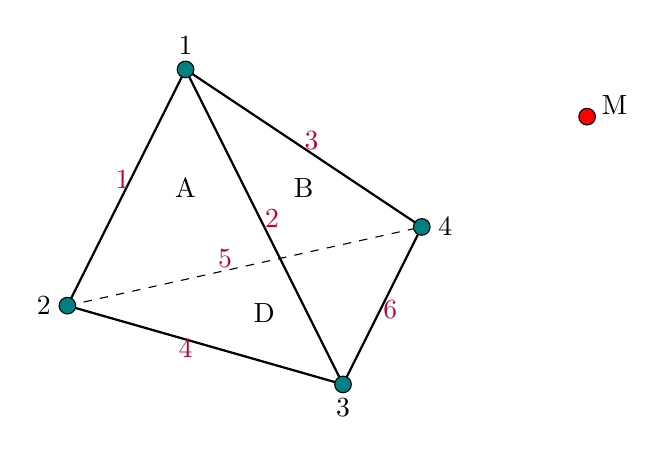
\begin{tikzpicture}
%\draw[step=0.5cm,gray,very thin] (0,0) grid (7,6); 
\draw[thick] (2.5,5) -- (1,2) -- (4.5,1) -- (5.5,3) -- cycle;
\draw[thick] (2.5,5)  -- (4.5,1) ;
\draw[dashed] (1,2) --  (5.5,3);
\node[] at (2.5,5.3) {$1$};
\node[] at (0.7,2) {$2$};
\node[] at (4.5,0.7) {$3$};
\node[] at (5.8,3) {$4$};
\draw[black,fill=teal] (2.5,5) circle (3pt);
\draw[black,fill=teal] (1,2) circle (3pt);
\draw[black,fill=teal] (4.5,1) circle (3pt);
\draw[black,fill=teal] (5.5,3) circle (3pt);
\node[] at (2.5,3.5) {A};
\node[] at (4,3.5) {B};
\node[] at (3.5,1.9) {D};
\draw[black,fill=red] (7.6,4.4) circle (3pt);
\node[] at (7.95,4.55) {M};
\node[] at (1.7,3.6) {\color{purple}1};
\node[] at (3.6,3.1) {\color{purple}2};
\node[] at (4.1,4.1) {\color{purple}3};
\node[] at (2.5,1.45) {\color{purple}4};
\node[] at (3,2.6) {\color{purple}5};
\node[] at (5.1,1.95) {\color{purple}6};
\end{tikzpicture}\\
{\captionfont Face C is hidden in the back.}
\end{center}


When looking at a face from the outside towards the tetrahedron the numbering 
of vertices is counter-clockwise.
\begin{center}
\begin{tabular}{ccccc}
\hline
face & vertices $i,j,k$ & edge \#1 & edge \#2 & edge \#3 \\
\hline\hline
A& 1,2,3  & 12({\color{purple}1}) & 23({\color{purple}4}) & 31({\color{purple}2}) \\
B& 1,3,4  & 13({\color{purple}2}) & 34({\color{purple}6}) & 41({\color{purple}3}) \\
C& 1,4,2  & 14({\color{purple}3}) & 42({\color{purple}5}) & 21({\color{purple}1}) \\
D& 2,4,3  & 24({\color{purple}5}) & 43({\color{purple}6}) & 32({\color{purple}4}) \\
\hline
edge & vertices & belongs to \\
{\color{purple}1} & 12 & A,C\\
{\color{purple}2} & 13 & A,B\\
{\color{purple}3} & 14 & B,C\\
{\color{purple}4} & 23 & A,D\\
{\color{purple}5} & 24 & C,D\\
{\color{purple}6} & 34 & B,D\\
\hline
\end{tabular}
\end{center}


\begin{center}
\begin{tikzpicture}
%\draw[step=0.5cm,gray,very thin] (0,0) grid (12,8.5); 
\draw[thick] (0.6,2.8) -- (3,5.6)--(6.7,6.9);
\draw[thick] (3,5.6)  -- (8.1,3.2) ;
\draw[thick] (5.9,0.4) -- (8.1,3.2) -- (11.1,4.2);
\node[] at (9,4.5) {face A};
\node[] at (4.5,2) {face B};
\draw[thick,->] (2.4,3.5)--(0.5,5); 
\node[] at (0.5,5.25) {$\vec{n}_B$};
\draw[] (2.2,3.65) -- (2.38,3.85) --(2.58,3.66);
\draw[thick,->] (5.5,5.7)--(5.2,8.1); 
\node[] at (5.6,8) {$\vec{n}_A$};
\draw[] (5.45,6) --(5.7,6.075) --(5.75,5.8);
\node[] at (2.7,5.7) {1};
\node[] at (8.2,2.85) {2};
\draw[black,fill=teal] (3,5.6) circle (3pt);
\draw[black,fill=teal] (8.1,3.2) circle (3pt);
\node[] at (8,5.8) {$\vec{n}_{21,B}$};
\draw[thick,->] (6.5,4)--(7.75,5.6); 
\node[] at (4,3) {$\vec{n}_{12,A}$};
\draw[thick,->] (6.5,4)--(4.1,3.2); 
\node[rotate=-25] at (5,5) {common edge};
\end{tikzpicture}\\
{\captionfont Figure made after Fig.~7 from \textcite{wesc97}.}
\end{center}



$\vec{n}_{1,A}=\vec{n}_{12,A}=(n_x,n_y)$ is such that it is perpendicular to $\vec{n}_A$ 
(it lies in the face $A$ plane), i.e. $\vec{n}_{1,A}\cdot \vec{n}_A=0$ and to edge $\#1$, i.e. 
$\vec{n}_{1,A}\cdot \vec{l}_{1}=0$. The cross product of $\vec{n}_A$ and $\vec{l}_{1}$ is 
by definition a vector perpendicular to both.
We also need to make sure it is pointing outwards. We then take the scalar product of a 
vector joining the center of the face and the middle of the 
edge under consideration. If it is negative then the normal is pointing towards the center of the 
face so it needs to be flipped.




%-------------------------------------------
\subsection*{Point mass approach}

Let us denote by $V$ the volume of the tetrahedron which 
can easily be computed:
\begin{equation}
V=\frac16 \left| (\vec{l}_{\color{purple}1} \times \vec{l}_{\color{purple}2}) \cdot \vec{l}_{\color{purple}3}\right|
\label{eq:tet:vol}
\end{equation}

\begin{center}
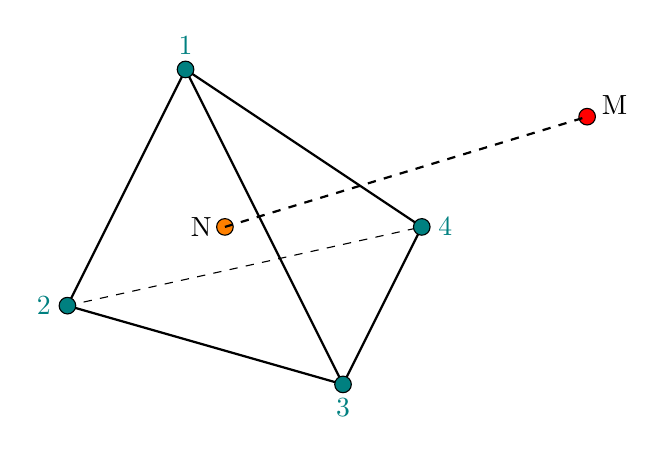
\begin{tikzpicture}
%\draw[step=0.5cm,gray,very thin] (0,0) grid (7,6); 
\draw[thick] (2.5,5) -- (1,2) -- (4.5,1) -- (5.5,3) -- cycle;
\draw[thick] (2.5,5)  -- (4.5,1) ;
\draw[dashed] (1,2) --  (5.5,3);
\node[] at (2.5,5.3) {\color{teal}$1$};
\node[] at (0.7,2) {\color{teal}$2$};
\node[] at (4.5,0.7) {\color{teal}$3$};
\node[] at (5.8,3) {\color{teal}$4$};
\draw[black,fill=teal] (2.5,5) circle (3pt);
\draw[black,fill=teal] (1,2) circle (3pt);
\draw[black,fill=teal] (4.5,1) circle (3pt);
\draw[black,fill=teal] (5.5,3) circle (3pt);

\draw[black,fill=orange] (3,3) circle (3pt);
\node[] at (2.7,3) {N};

\draw[black,fill=red] (7.6,4.4) circle (3pt);
\node[] at (7.95,4.55) {M};

\draw[thick,dashed] (3,3)--(7.6,4.4);

\end{tikzpicture}
\end{center}


The coordinates of its center of gravity $N$ are given 
by 
\begin{equation}
x_N= \frac{1}{4}(x_{\color{teal}1}+x_{\color{teal}2}+x_{\color{teal}3}+x_{\color{teal}4})
\qquad
y_N= \frac{1}{4}(y_{\color{teal}1}+y_{\color{teal}2}+y_{\color{teal}3}+y_{\color{teal}4})
\qquad
z_N= \frac{1}{4}(z_{\color{teal}1}+z_{\color{teal}2}+z_{\color{teal}3}+z_{\color{teal}4})
\label{eq:tet:centerN}
\end{equation}
If the tetrahedron is considered a point mass, then 
the gravity field and potential are given by
\begin{eqnarray}
\vec{g}_{pm} &=& {\cal G}  \frac{\rho_0 V}{|\overrightarrow{MN}|^3} \overrightarrow{MN}
\\
U_{pm} &=& {\cal G}  \frac{\rho_0 V}{|\overrightarrow{MN}|} 
\end{eqnarray}
with 
\[
\overrightarrow{MN} =
\left(
\begin{array}{c}
x_N - x_M \\
y_N - y_M \\
z_N - z_M 
\end{array}
\right)
\]

Function \verb|compute_gravity_tetrahedron_pointmass| receives coordinates of the four vertices {\color{teal}1}, {\color{teal}2}, {\color{teal}3}, {\color{teal}4},  its density and the coordinates of the measurement point.

\begin{enumerate}
\item compute coordinates $x_N,y_N,z_N$ of center of gravity with Eq.~\eqref{eq:tet:centerN}
$\rightarrow$ \verb|xN,yN,zN|

\item compute volume $V$ of tetrahedron with Eq.~\ref{eq:tet:vol}$ \rightarrow$ \verb|Vol| 
\item compute $\vec{g}_{pm}$
\end{enumerate}







%--------------------------------
\subsection*{Full tetrahedron}

Function \verb|compute_gravity_tetrahedron| receives coordinates of the four vertices {\color{teal}1}, 
{\color{teal}2}, {\color{teal}3}, {\color{teal}4}, its density $\rho_0$ and the coordinates of the 
measurement point $M$.

I do not like the notation $\vec{e}_{12}$ for an edge vector since in fieldstone $\vec{e}$ is always 
a unit vector for the coordinate system. I then rename edge vectors $\vec{l}$.

The structure of the function goes as follows:
\begin{enumerate}
\item compute $\vec{l}_{\color{purple}1}$, $\vec{l}_{\color{purple}2}$,etc ... and their norms 
$\rightarrow$ \verb|vec_l1|, \verb|vec_l2|, \verb|vec_l3|, \verb|vec_l4|, \verb|vec_l5|, \verb|vec_l6|

\[
\vec{l}_{\color{purple}1} = \vec{l}_{\color{teal}12} = \left(
\begin{array}{c}
x_{\color{teal}2}-x_{\color{teal}1} \\
y_{\color{teal}2}-y_{\color{teal}1} \\
z_{\color{teal}2}-z_{\color{teal}1}
\end{array}
\right)
\qquad
\vec{l}_{\color{purple}2} = \vec{l}_{\color{teal}13} = \left(
\begin{array}{c}
x_{\color{teal}3}-x_{\color{teal}1} \\
y_{\color{teal}3}-y_{\color{teal}1} \\
z_{\color{teal}3}-z_{\color{teal}1}
\end{array}
\right)
\qquad
\textrm{etc...}
\]


\item compute $\vec{r}_{\color{teal} 1,2,3,4}$. $\rightarrow$ \verb|vec_r1|, \verb|vec_r2|, \verb|vec_r3|, \verb|vec_r4|
\[
\vec{r}_{\color{teal}1} = \vec{M1} = \left(
\begin{array}{c}
x_{\color{teal}1}-x_m \\
y_{\color{teal}1}-y_m \\
z_{\color{teal}1}-z_m
\end{array}
\right)
\]



\item compute $\vec{n}_{A,B,C,D}$. 
$\rightarrow$ \verb|vec_nA| , \verb|vec_nB|, \verb|vec_nC|, \verb|vec_nD|

\begin{eqnarray}
\vec{n}_A 
&=& \vec{l}_{\color{teal}12}\times\vec{l}_{\color{teal}13}/|\vec{l}_{\color{teal}12}\times\vec{l}_{\color{teal}13}|
= \vec{l}_{\color{purple}1}\times\vec{l}_{\color{purple}2}/| \vec{l}_{\color{purple}1}\times\vec{l}_{\color{purple}2}| \\
\vec{n}_B 
&=& \vec{l}_{\color{teal}13}\times\vec{l}_{\color{teal}14}/|\vec{l}_{\color{teal}13}\times\vec{l}_{\color{teal}14}|
= \vec{l}_{\color{purple}2}\times\vec{l}_{\color{purple}3}/|\vec{l}_{\color{purple}2}\times\vec{l}_{\color{purple}3}|  \\
\vec{n}_C 
&=& \vec{l}_{\color{teal}14}\times\vec{l}_{\color{teal}12}/|\vec{l}_{\color{teal}14}\times\vec{l}_{\color{teal}12}|   
= \vec{l}_{\color{purple}3}\times\vec{l}_{\color{purple}1}/|\vec{l}_{\color{purple}3}\times\vec{l}_{\color{purple}1}|   \\
\vec{n}_D 
&=& \vec{l}_{\color{teal}24}\times\vec{l}_{\color{teal}23}/|\vec{l}_{\color{teal}24}\times\vec{l}_{\color{teal}23}|   
= \vec{l}_{\color{purple}5}\times\vec{l}_{\color{purple}4}/|\vec{l}_{\color{purple}5}\times\vec{l}_{\color{purple}4}|
\end{eqnarray}


\item compute ${\bm F}_{A,B,C,D}$. 
$\rightarrow$ \verb|mat_FA| , \verb|mat_FB|, \verb|mat_FC|, 
\verb|mat_FD|

\begin{eqnarray}
{\bm F}_A &=& \vec{n}_A\vec{n}_A \\
{\bm F}_B &=& \vec{n}_B\vec{n}_B \\
{\bm F}_C &=& \vec{n}_C\vec{n}_C \\
{\bm F}_D &=& \vec{n}_D\vec{n}_D 
\end{eqnarray}

\item compute $\omega_{A,B,C,D}$. $\rightarrow$ \verb|wA| , \verb|wB|, \verb|wC|, \verb|wD|

\begin{eqnarray}
\omega_A &=& 
2 \arctan \frac{\vec{r_{\color{teal}1}} \cdot (\vec{r}_{\color{teal}2} \times \vec{r}_{\color{teal}3})}{r_{\color{teal}1}r_{\color{teal}2}r_{\color{teal}3} 
+r_{\color{teal}1}(\vec{r}_{\color{teal}2}\cdot\vec{r}_{\color{teal}3}) 
+r_{\color{teal}2}(\vec{r}_{\color{teal}3}\cdot\vec{r}_{\color{teal}1}) 
+r_{\color{teal}3}(\vec{r}_{\color{teal}1}\cdot\vec{r}_{\color{teal}2})  } \nn\\
\omega_B &=& 
2 \arctan \frac{\vec{r_{\color{teal}1}} \cdot (\vec{r}_{\color{teal}3} \times \vec{r}_{\color{teal}4})}{r_{\color{teal}1}r_{\color{teal}3}r_{\color{teal}4} 
+r_{\color{teal}1}(\vec{r}_{\color{teal}3}\cdot\vec{r}_{\color{teal}4}) 
+r_{\color{teal}3}(\vec{r}_{\color{teal}4}\cdot\vec{r}_{\color{teal}1}) 
+r_{\color{teal}4}(\vec{r}_{\color{teal}1}\cdot\vec{r}_{\color{teal}3})  } \nn\\
\omega_C &=&
2 \arctan \frac{\vec{r_{\color{teal}1}} \cdot (\vec{r}_{\color{teal}4} \times \vec{r}_{\color{teal}2})}{r_{\color{teal}1}r_{\color{teal}4}r_{\color{teal}2}
+r_{\color{teal}1}(\vec{r}_{\color{teal}4}\cdot\vec{r}_{\color{teal}2}) 
+r_{\color{teal}4}(\vec{r}_{\color{teal}2}\cdot\vec{r}_{\color{teal}1}) 
+r_{\color{teal}2}(\vec{r}_{\color{teal}1}\cdot\vec{r}_{\color{teal}4}) 
} \nn\\
\omega_D &=&
2 \arctan \frac{\vec{r_{\color{teal}2}} \cdot (\vec{r}_{\color{teal}4} \times \vec{r}_{\color{teal}3})}{r_{\color{teal}2}r_{\color{teal}4}r_{\color{teal}3} 
+r_{\color{teal}2}(\vec{r}_{\color{teal}4}\cdot\vec{r}_{\color{teal}3}) 
+r_{\color{teal}4}(\vec{r}_{\color{teal}3}\cdot\vec{r}_{\color{teal}2}) 
+r_{\color{teal}3}(\vec{r}_{\color{teal}2}\cdot\vec{r}_{\color{teal}4}) 
}
\end{eqnarray}


\item compute $\vec{r}_{A}$, $\vec{r}_{B}$, $\vec{r}_{C}$, $\vec{r}_{D}$.
As explained in the caption of their Figure~3, ``vector $\vec{r}_f$
extends from the field point $M$ to any point in the face plane''.
$\rightarrow$ \verb|vec_rA|, \verb|vec_rB|, \verb|vec_rC|, \verb|vec_rD|

\item compute $\vec{g}_f$ by means of % Eq.~\eqref{eq:tetra:gf}

\[
\vec{g}_f
= {\cal G} \rho_0 \sum_f \omega_f {\bm F}_f\cdot \vec{r}_f \nn\\
= {\cal G} \rho_0 \left(
\omega_A {\bm F}_A\cdot \vec{r}_A +
\omega_B {\bm F}_B\cdot \vec{r}_B +
\omega_C {\bm F}_C\cdot \vec{r}_C +
\omega_D {\bm F}_D\cdot \vec{r}_D 
\right)\label{eq:tetra:gf}
\]




\item compute $\vec{n}_{e,f}$ for each edge of each face (12 vectors!)
$\rightarrow$ \verb|vec_nA12|, \verb|vec_nA23|, \verb|vec_nA13|, \verb|vec_nB13|, etc ...


\item compute ${\bm E}_{\color{purple} 1,2,3,4,5,6}$. 
$\rightarrow$ \verb|mat_E12, mat_E13, mat_E14, mat_E23, mat_E24, mat_E34| 

\begin{eqnarray}
{\bm E}_{\color{purple}1} ={\bm E}_{\color{teal}12}
&=&\vec{n}_A \vec{n}_{{\color{teal}12},A} +\vec{n}_C \vec{n}_{{\color{teal}21},C}\\
{\bm E}_{\color{purple}2} ={\bm E}_{\color{teal}13}
&=& \vec{n}_A \vec{n}_{{\color{teal}13},A} +\vec{n}_B \vec{n}_{{\color{teal}13},B} \\
{\bm E}_{\color{purple}3} ={\bm E}_{\color{teal}14}
&=& \vec{n}_B \vec{n}_{{\color{teal}14},B}+\vec{n}_C \vec{n}_{{\color{teal}14},C} \\
{\bm E}_{\color{purple}4} ={\bm E}_{\color{teal}23}
&=& \vec{n}_A \vec{n}_{{\color{teal}23},A}+\vec{n}_D \vec{n}_{{\color{teal}23},D} \\
{\bm E}_{\color{purple}5} ={\bm E}_{\color{teal}24}
&=& \vec{n}_C \vec{n}_{{\color{teal}24},C} +\vec{n}_D \vec{n}_{{\color{teal}24},D} \\  
{\bm E}_{\color{purple}6} ={\bm E}_{\color{teal}34}
&=& \vec{n}_B \vec{n}_{{\color{teal}34},B} +\vec{n}_D \vec{n}_{{\color{teal}34},D} 
\end{eqnarray}



\item compute $L_{\color{purple}1,2,3,4,5,6}$ $\rightarrow$ \verb|L12|, \verb|L13|, \verb|L14|, ...
\begin{eqnarray}
L_{\color{purple}1} = L_{\color{teal}12} 
&=& \ln \frac{r_{\color{teal}1}+r_{\color{teal}2}+l_{\color{purple}1}}{r_{\color{teal}1}+r_{\color{teal}2}-l_{\color{purple}1}} \nn\\
L_{\color{purple}2} = L_{\color{teal}13} 
&=& \ln \frac{r_{\color{teal}1}+r_{\color{teal}3}+l_{\color{purple}2}}{r_{\color{teal}1}+r_{\color{teal}3}-l_{\color{purple}2}} \nn\\
L_{\color{purple}3} = L_{\color{teal}14} 
&=& \ln \frac{r_{\color{teal}1}+r_{\color{teal}4}+l_{\color{purple}3}}{r_{\color{teal}1}+r_{\color{teal}4}-l_{\color{purple}3}} \nn\\
L_{\color{purple}4} = L_{\color{teal}23} 
&=& \ln \frac{r_{\color{teal}2}+r_{\color{teal}3}+l_{\color{purple}4}}{r_{\color{teal}2}+r_{\color{teal}3}-l_{\color{purple}4}} \nn\\
L_{\color{purple}5} = L_{\color{teal}24} 
&=& \ln \frac{r_{\color{teal}2}+r_{\color{teal}4}+l_{\color{purple}5}}{r_{\color{teal}2}+r_{\color{teal}4}-l_{\color{purple}5}} \nn\\
L_{\color{purple}6} = L_{\color{teal}34} 
&=& \ln \frac{r_{\color{teal}3}+r_{\color{teal}4}+l_{\color{purple}6}}{r_{\color{teal}3}+r_{\color{teal}4}-l_{\color{purple}6}} \nn
\end{eqnarray}


\item compute $\vec{r}_{\color{teal}12,13,14,23,24,34}$. As specified in Section~2.1.8 of their paper ``$\vec{r}_e$ is a vector from the field point to any point on edge $e$ or its infinite extension''
$\rightarrow$ \verb|vec_r12|, \verb|vec_r13|, \verb|vec_r13|, etc ...  


\item compute $\vec{g}_e$ by means of Eq.~\eqref{eq:tetra:ge}

\[
\vec{g}_e 
={\cal G} \rho_0 \sum_e L_e {\bm E}_e \cdot \vec{r}_e 
={\cal G} \rho_0 \left( 
L_{\color{teal}12} {\bm E}_{\color{teal}12}\cdot\vec{r}_{\color{teal}12} +
L_{\color{teal}13} {\bm E}_{\color{teal}23}\cdot\vec{r}_{\color{teal}13} +
L_{\color{teal}14} {\bm E}_{\color{teal}34}\cdot\vec{r}_{\color{teal}14} +
L_{\color{teal}23} {\bm E}_{\color{teal}23}\cdot\vec{r}_{\color{teal}23} 
L_{\color{teal}24} {\bm E}_{\color{teal}24}\cdot\vec{r}_{\color{teal}24} 
L_{\color{teal}34} {\bm E}_{\color{teal}34}\cdot\vec{r}_{\color{teal}34} 
\right)
\]


\item compute $\vec{g}=-\vec{g}_e+\vec{g}_f$

\end{enumerate}

Except for the 4 measurements provided in \textcite{mequ86} I could not easily find 
actual values to benchmark the code against, so the following three examples aim at 
remedying this problem. 
In all what follows we set $\rho_0=1$ and ${\cal G}=1$.

%..............................................
\subsection*{test 1: the Wikipedia tetrahedron}

We consider the following regular tetrahedron (i.e. all faces are equilateral triangles) centered at the 
origin\footnote{\url{https://en.wikipedia.org/wiki/Tetrahedron}}. Its edges are $l=\sqrt{8/3}$ long.
We have
\begin{eqnarray}
(x_1,y_1,z_1) &=& (0,0,1) \nn\\
(x_2,y_2,z_2) &=& (\sqrt{8/9},0,-1/3) \nn\\
(x_3,y_3,z_3) &=& (-\sqrt{2/9},\sqrt{2/3},-1/3) \nn\\
(x_4,y_4,z_4) &=& (-\sqrt{2/9},-\sqrt{2/3},-1/3) \nn
\end{eqnarray}
Point 1 is at the top and points 2,3,4 are in the $z=-1/3$ plane.

\begin{center}
\includegraphics[width=5cm]{python_codes/fieldstone_113/images/tet1}
\end{center}

The volume of a regular tetrahedron of edge $l$ is given by:
\[
V=\frac{l^3}{6\sqrt{2}} = \frac{8}{9\sqrt{3}} \simeq 0.5132
\]
and this is what we indeed recover.


%..............................................
\subsection*{test 2: the 111-tetrahedron}

It is defined in \textcite{mequ86} (1986) (with a correction by \textcite{camq86} (1986)).

\begin{center}
\includegraphics[width=8cm]{python_codes/fieldstone_113/images/mequ86a}
\end{center}

In this case I choose pt1 is node C, pt2 is H, pt3 is F pt 4 is A.
If the cube is a unit cube then the edge length is $\sqrt{2}$ and the volume
\[
V=\frac{l^3}{6\sqrt{2}} = \frac13
\]

\begin{center}
\includegraphics[width=5cm]{python_codes/fieldstone_113/images/tet2}
\end{center}

\textcite{mequ86} state: ``To ensure that the above analysis can be treated
with confidence we have performed numerical calculations of the field components Fx, Fy, and 
Fz using the expressions developed in this paper and
have compared them with those obtained by direct numerical integration'':
\begin{center}
\includegraphics[width=5cm]{python_codes/fieldstone_113/images/mequ86b}\\
{\captionfont Taken from \textcite{mequ86}.}
\end{center}

\begin{center}
\begin{tabular}{lllcc}
\hline
$x$ & $y$ & $z$ & $g_x$ (tet) & $g_x$ (point mass) \\
\hline
\hline
1.25 & 0.5 & 0.5 &  0.566679144260546  & 0.5925925925925926 \\
1.5  & 0.5 & 0.5 &  0.326526930616740  & 0.3333333333333333 \\
1.75 & 0.5 & 0.5 &  0.211222015971550  & 0.2133333333333333 \\
2.0  & 0.5 & 0.5 &  0.147377525744174  & 0.1481481481481481 \\
\hline
\end{tabular}\\
Results obtained with Stone 113
\end{center}

Gravity fields are measured on a line starting at $(1,0.5,0.5)$ and ending at $(5,0.5,0.5)$
\begin{center}
\includegraphics[width=7cm]{python_codes/fieldstone_113/results/test2/g_vector.pdf}
\includegraphics[width=7cm]{python_codes/fieldstone_113/results/test2/g_vector_diff.pdf}\\
\includegraphics[width=7cm]{python_codes/fieldstone_113/results/test2/g_pot.pdf}
\includegraphics[width=7cm]{python_codes/fieldstone_113/results/test2/g_pot_diff.pdf}
\end{center}





%..........................................
\subsection*{test 3: the origin tetrahedron}

This is not a regular tetrahedron since $l_{1} \neq l_4 $.

\begin{center}
\includegraphics[width=5cm]{python_codes/fieldstone_113/images/tet3}
\end{center}


\begin{eqnarray}
(x_1,y_1,z_1) &=& (0,0,0) \nn\\
(x_2,y_2,z_2) &=& (1,0,0) \nn\\ 
(x_3,y_3,z_3) &=& (0,1,0) \nn\\
(x_4,y_4,z_4) &=& (0,0,1) \nn
\end{eqnarray}

The gravity fields are measured on a line starting at $(1,1,1)$ and ending at $(3,3,3)$:

\begin{center}
\includegraphics[width=7cm]{python_codes/fieldstone_113/results/test3/g_vector.pdf}
\includegraphics[width=7cm]{python_codes/fieldstone_113/results/test3/g_vector_diff.pdf}\\
\includegraphics[width=7cm]{python_codes/fieldstone_113/results/test3/g_pot.pdf}
\includegraphics[width=7cm]{python_codes/fieldstone_113/results/test3/g_pot_diff.pdf}
\end{center}


%.................................................
\subsection*{test 4: cube containing 5 tetrahedra}




%..............................................
\subsection*{test 5: sphere made of tetrahedra}








 %%%%%%%%%%%%%%%%%%%%%%%%%%%%%%%%%%%%%%%%%%%%%%%%%

\newpage %%%%%%%%%%%%%%%%%%%%%%%%%%%%%%%%%%%%%%%%%%%%%%%%%%%%%%%%%%%%%%%%%%%%%%%%%%%%%%%%
\section*{
Stone 114: Joint Gravity and Stokes inversion of a 2D circular anomaly 
\label{f114}}
\addcontentsline{toc}{section}{\protect\numberline{} 
Stone 114: Joint Gravity and Stokes inversion of a 2D circular anomaly
}
\begin{flushright} {\tiny {\color{gray} python\_codes/fieldstone\_114/text.tex}} \end{flushright}

%\lstinputlisting[language=bash,basicstyle=\small]{python_codes/fieldstone_114/keywords}

\begin{center}
\fbox{\textbf{\huge \color{teal} P}}
Codes at \url{https://github.com/cedrict/fieldstone/tree/master/python_codes/fieldstone_114}
\end{center}

\par\noindent\rule{\textwidth}{0.4pt}

{\sl The python stone was developed in collaboration with W. Klessens}. \index{contributors}{W. Klessens}
{\sl The julia stone was developed in collaboration with J. Jansen}. \index{contributors}{J. Jansen}

\par\noindent\rule{\textwidth}{0.4pt}
%%%%%%%%%%%%%%%%%%%%%%%%%%%%%%%%%%%%%%%%%%%%%%%%%%%%%%%%%%%%%%%%%%%%%%%%%%%%%%%%%%%%%%%%%%%%%%

This \stone is inspired by \textcite{bakp14} (2014).
The setup is as follows:

\begin{center}
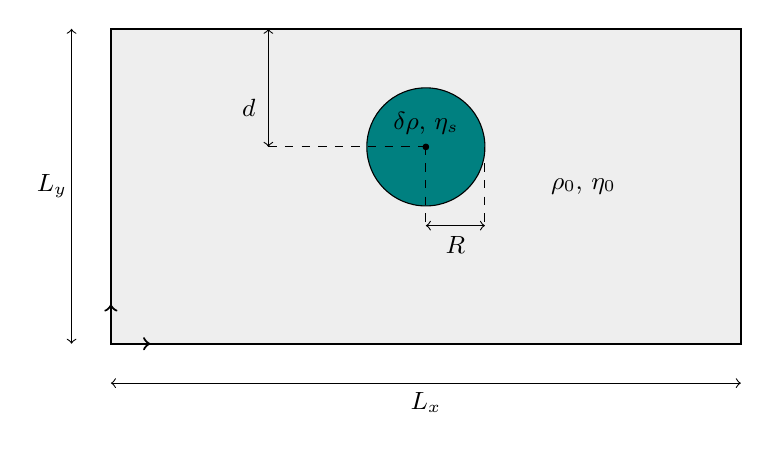
\begin{tikzpicture}
%\draw[step=0.5cm,gray,very thin] (0,0) grid (10,6); %background grid
\draw[fill=gray!63,gray!13](1,1) rectangle (9,5);
\draw[thick] (1,1) -- (9,1) -- (9,5) -- (1,5) -- cycle; %top
\draw[black,fill=teal] (5,3.5)   circle (0.75cm);
\draw[thick,->] (1,1) -- (1.5,1); 
\draw[thick,->] (1,1) -- (1,1.5); 
\draw[black,fill=black] (5,3.5)   circle (1pt);
\draw[thin,<->] (0.5,1) -- (0.5,5); 
\draw[thin,<->] (1,0.5) -- (9,0.5); 
\draw[thin,<->] (3,3.5) -- (3,5); 
\draw[thin,<->] (5,2.5) -- (5.75,2.5); 
\node[] at (5,0.25) {\small $L_x$};
\node[] at (0.25,3) {\small $L_y$};
\node[] at (2.75,4) {\small $d$};
\node[] at (5.375,2.25) {\small $R$};
\draw[dashed,thin] (3,3.5)--(5,3.5);
\draw[dashed,thin] (5,3.5)--(5,2.5);
\draw[dashed,thin] (5.75,3.5)--(5.75,2.5);
\node[] at (7,3) {\small $\rho_0$, $\eta_0$};
\node[] at (5,3.8) {\small $\delta\rho$, $\eta_s$};
\end{tikzpicture}
\end{center}

When the sphere is lighter than its surrounding it goes up and creates a 
divergent flow at the surface. As explained in \textcite{bakp14} an analytical 
solution exists for the horizontal component of the velocity at the surface in 3D. 
Also, the lower density of the sphere (or rather the density difference $\delta\rho$
between the sphere and its surrounding) yields a gravity field 
above the sphere that is lower and for which an analytical solution exists too.

Assuming we have determined what the depth of the sphere is (and assuming that 
it is rigid by taking its viscosity $\eta_s >> \eta_0$), then the two main 
+unknowns are its density difference $\delta \rho$ with regard to the surrounding mantle
and its radius $R$. 

To start with, we can compute analytically the gravity and velocity that a 
$\delta\rho^\dag=-300$ and $R^\dag=50~\si{\km}$ disc generates at the surface of the model,
write a simple inversion code which would operate in the $(R,\delta\rho)$-space 
and automatically looks for the real values of the sphere by computing a gravity misfit $\xi_g$ 
and velocity misfit $\xi_v$ and using these quantities to zero-in on the correct values 
of $\delta \rho$ and $R$.


Three ideas:

- axisymmetric

- full 3D

- try JIT? julia?


%--------------------------------------------------------
\subsection*{gravity forward model - analytical solution}

We consider a circular inclusion at half the 2D domain of 
$1000~\si{\km}$ in $x$- and $500~\si{\km}$ in $y$-direction. 
Because of the evident symmetry of the problem we restrict the 
calculations to the right half of the domain so that now it 
is a square of size $L_x=L_y=500~\si{\km}$ and the sphere is 
at coordinates $(x_c,y_c)=(0,Ly/2)$.

In the case of a disc, the gravity in the $x,y-$plane is given by 
\[
\vec{g}(x,y) = {\cal G} \frac{\pi R^2 \delta\rho}{(x-x_c)^2+(y-y_c)^2} 
\left(
\begin{array}{c}
x-x_c \\
y-y_c
\end{array}
\right)
\]
In the case of a sphere, 
\[
\vec{g}(x,y,z) = {\cal G} \frac{\pi R^2 \delta\rho}{(x-x_c)^2+(y-y_c)^2+(z-z_c)^2} 
\left(
\begin{array}{c}
x-x_c \\
y-y_c \\
z-z_c 
\end{array}
\right)
\]
Gravity is computed by transforming the integral 
\[
\vec{g}(x,y) = \iiint_V {\cal G} \frac{\rho(x',y',z')}{ (x-x')^2+(y-y')^2+(z-z')^2    } dx'dy'dz'
\]
over the domain by a sum of elemental 
integrals which are then computed by means of the same quadrature as the FE matrix. 
Since half the disk is missing, we on-the-fly take the missing half into account by 
mirroring the quadrature points and adding their contribution. 

Because we are only interested in the gravity signal generated by the disc/sphere, 
a boolean array {\tt elt\_in\_sphere} is created and set to true for those elements
for which at least one quadrature point is inside the sphere. This array is then used
to target the contribution of the elements 'inside' the sphere. 



%--------------------------------------------------------
\subsection*{Stokes forward model - analytical solution}

The surface velocity signal of a rising sphere is computed in Appendix~A of \textcite{bakp14} (2014).
It is based on \textcite{bren61} (1961), \textcite{stje26} (1926) and \textcite{pacy05} (2005). See also 
\textcite{burg16} (1916). The solution is only available in 3D with axisymmetric geometry. 
The analytical expression is rather complex and in order to keep simple for now, we
will use a different reference velocity quantity to carry out the inversion. 
In the folder {\tt reference\_code} a modified version of \stone~2 is placed. 
It computes the velocity field for the reference case
at a 150x150 resolution. The root mean square velocity 
$\upnu_{rms}=7.740432578645655e-10~\si{\meter\per\second}$ 
will serve as our reference value to drive the inversion.

\begin{center}
\includegraphics[width=6cm]{python_codes/fieldstone_114/reference_code/vel}
\includegraphics[width=6cm]{python_codes/fieldstone_114/reference_code/eta}\\
{\captionfont Sphere radius is $R=50~\si{\km}$, $\rho_m=3000$, $\delta\rho=-300$, $\eta^\star=10^3$.}
\end{center}

%--------------------------------------------------------
\subsection*{The code}

In order to produce a reasonably fast Stokes solver the code relies on 
the $Q_1\times P_0$ element with a penalty approach (see for example \stone~01).
The Cartesian domain is overlain with a mesh counting $nel_x\times nel_y=nel$
elements which are all square, so that the Jacobian of the transformation
between global and local coordinates is diagonal. Its value has been 
hard-wired in the code so as to save time. 
The entire Stokes solver + gravity calculator is inserted into a single function
{\tt compute\_misfits} in the {\pythonfile forward.py} file.

Note that depending on the mesh resolution a call to the function will take betweem 1s 
(50x50) 2.5s (64x64), and 8s (100x100). 

%--------------------------------------------------------
\subsection*{Inversion}

The first inversion code {\pythonfile driver1.py} is very simple. The user defines the bounds of the 
parameter space, i.e. $\delta\rho_{min}$, $\delta\rho_{max}$, $R_{min}$ and $R_{max}$.
Then a regular grid composed of $n_{\delta\rho} \times n_{R}$ is used to compute 
both misfits $\xi_g$ and $\xi_v$ at each node of the grid and these are 
exported in a vtu file. No refinement or clever search takes place. 

\begin{center}
\includegraphics[width=5.7cm]{python_codes/fieldstone_114/results/min}
\includegraphics[width=5.7cm]{python_codes/fieldstone_114/results/mg}
\includegraphics[width=5.7cm]{python_codes/fieldstone_114/results/mv}\\
{\captionfont horizontal axis is radius $R$, vertical axis is $\delta\rho$. 60x60 points. about 2.5h.
Left: location of the true minimum, i.e. the reference model; Middle: gravity misfit; Right: vrms misfit.} 
\end{center}




 %%%%%%%%%%%%%%%%%%%%%%%%%%%%%%%%%%%%%%%%%%%%%%%%%

\newpage %%%%%%%%%%%%%%%%%%%%%%%%%%%%%%%%%%%%%%%%%%%%%%%%%%%%%%%%%%%%%%%%%%%%%%%%%%%%%%%%
\section*{
Stone 115: $Q_1\times P_0$-stab element for isoviscous flow
\label{f115}}
\addcontentsline{toc}{section}{\protect\numberline{} 
Stone 115: $Q_1\times P_0$-stab element for isoviscous flow
}
\begin{flushright} {\tiny {\color{gray} python\_codes/fieldstone\_115/text.tex}} \end{flushright}

\lstinputlisting[language=bash,basicstyle=\small]{python_codes/fieldstone_115/keywords}

\begin{center}
\fbox{\textbf{\huge \color{teal} P}}
Codes at \url{https://github.com/cedrict/fieldstone/tree/master/python_codes/fieldstone_115}
\end{center}

\par\noindent\rule{\textwidth}{0.4pt}

%%%%%%%%%%%%%%%%%%%%%%%%%%%%%%%%%%%%%%%%%%%%%%%%%%%%%%%%%%%%%%%%%%%%%%%%%%%%%%%%%%%%%%%%%%%%%%



When it comes to the stabilisation of the $Q_1\times P_0$ elements, 
we have seen in Section~\ref{ss:pairq1p0stab} that mulitple types co-exist
and that a tuning parameter $\epsilon$ plays a role. 
Despite the published literature on the topic, the following questions remain:

- how to deal with vicosity contrasts ? 

- which stab is best for real life geodynamics ? 

- how to deal with not square mesh ?

- how to choose the $\epsilon$ value ?

- look at buoyancy driven flows. lith pressure!

- I have implemented penalty, global, local and macro-element. what about the other methods, eg bodg06 ?

- concretely how would PCG converge?

The code is based on \stone 14.

Velocity divergence is measured at the center of the element.

note that in case of penalty, $\epsilon$ should be $\sim 10^6$ larger than viscosity.

%====================================================================================
\subsection*{Donea \& Huerta manufactured solution}


\begin{center}
\includegraphics[width=5cm]{python_codes/fieldstone_115/results/dh/nostab/matrix}
\includegraphics[width=5cm]{python_codes/fieldstone_115/results/dh/penalty/matrix}
\includegraphics[width=5cm]{python_codes/fieldstone_115/results/dh/global/matrix}\\
\includegraphics[width=5cm]{python_codes/fieldstone_115/results/dh/local/matrix}
\includegraphics[width=5cm]{python_codes/fieldstone_115/results/dh/macro/matrix}\\
{\captionfont 32x32. From left to right: parsity pattern of the FEM matric for 
no stabilisation, penalty, global, local, macro-elt.}
\end{center}

We find that all three stabilisation $\C$ matrices are enough to suppress the chequerboard mode:
\begin{center}
\includegraphics[width=5cm]{python_codes/fieldstone_115/results/dh/p0}
\includegraphics[width=5cm]{python_codes/fieldstone_115/results/dh/p1}
\includegraphics[width=5cm]{python_codes/fieldstone_115/results/dh/p2}\\
\includegraphics[width=5cm]{python_codes/fieldstone_115/results/dh/p3}
\includegraphics[width=5cm]{python_codes/fieldstone_115/results/dh/p4}\\
{\captionfont 32x32. From left to right: no stabilisation, penalty, global, local, macro-elt. $\epsilon=10^{-1}$}
\end{center}

We can now explore the influence of the stabilisation parameter $\epsilon$. Obviously, 
if too low it won't have any effect as the $\C$ matrix then tends to zero. If too high,
then we expect it to perturb the solution too much. 
The pressure field is shown in the following figure for various values of $\epsilon$, 


\begin{center}
\includegraphics[width=3.4cm]{python_codes/fieldstone_115/results/dh/pressure_nostab.pdf}
\includegraphics[width=3.4cm]{python_codes/fieldstone_115/results/dh/pressure_penalty.pdf}
\includegraphics[width=3.4cm]{python_codes/fieldstone_115/results/dh/pressure_global.pdf}
\includegraphics[width=3.4cm]{python_codes/fieldstone_115/results/dh/pressure_local.pdf}
\includegraphics[width=3.4cm]{python_codes/fieldstone_115/results/dh/pressure_macro.pdf}\\
\includegraphics[width=3.4cm]{python_codes/fieldstone_115/results/dh/pressure_nostab_error.pdf}
\includegraphics[width=3.4cm]{python_codes/fieldstone_115/results/dh/pressure_penalty_error.pdf}
\includegraphics[width=3.4cm]{python_codes/fieldstone_115/results/dh/pressure_global_error.pdf}
\includegraphics[width=3.4cm]{python_codes/fieldstone_115/results/dh/pressure_local_error.pdf}
\includegraphics[width=3.4cm]{python_codes/fieldstone_115/results/dh/pressure_macro_error.pdf}\\
{\captionfont 32x32. pressure profile.} 
\end{center}

Let us now turn to the velocity and pressure error convergence rates: 
\begin{center}
\includegraphics[width=4cm]{python_codes/fieldstone_115/results/dh/errorsV_penalty.pdf}
\includegraphics[width=4cm]{python_codes/fieldstone_115/results/dh/errorsV_global.pdf}
\includegraphics[width=4cm]{python_codes/fieldstone_115/results/dh/errorsV_local.pdf}
\includegraphics[width=4cm]{python_codes/fieldstone_115/results/dh/errorsV_macro.pdf}\\
\includegraphics[width=4cm]{python_codes/fieldstone_115/results/dh/errorsP_penalty.pdf}
\includegraphics[width=4cm]{python_codes/fieldstone_115/results/dh/errorsP_global.pdf}
\includegraphics[width=4cm]{python_codes/fieldstone_115/results/dh/errorsP_local.pdf}
\includegraphics[width=4cm]{python_codes/fieldstone_115/results/dh/errorsP_macro.pdf}\\
\includegraphics[width=4cm]{python_codes/fieldstone_115/results/dh/divv_penalty.pdf}
\includegraphics[width=4cm]{python_codes/fieldstone_115/results/dh/divv_global.pdf}
\includegraphics[width=4cm]{python_codes/fieldstone_115/results/dh/divv_local.pdf}
\includegraphics[width=4cm]{python_codes/fieldstone_115/results/dh/divv_macro.pdf}\\
{\captionfont Velocity and pressure errors as a function of the element size for meshes 6x6 to 128x128.
Left is penalty, middle is global, right is local.}
\end{center}
We find that the error convergence rate for velocity is always quadratic as expected, 
while the error convergence for pressure becomes monotonous and linear as expected too.

It also appears that the macro-element technique is the least sensitive to the value of $\epsilon$, 
although it is rather surprising that even very low values of $\epsilon$ manage to stabilise the 
system so well. could it be because this benchmark is very smooth? 
\begin{center}
\includegraphics[width=5.7cm]{python_codes/fieldstone_115/results/dh/errorsP_32_eps}
\includegraphics[width=5.7cm]{python_codes/fieldstone_115/results/dh/errorsP_64_eps}
\includegraphics[width=5.7cm]{python_codes/fieldstone_115/results/dh/errorsP_96_eps}\\
{\captionfont Influence of $\epsilon$ parameter on pressure error for global, local, macro-elt}
\end{center}

{\bf Conclusion}: macro-element technique yields best results: lower velocity divergence, 
least sensitive to $\epsilon$ value, block matrix,

I should monitor the condition number of the matrix...

\newpage
%====================================================================================
\subsection*{The aquarium}

The domain is still a unit square. Boundary conditions are no slip on all sides. 
Density and viscosity are set to 1. Gravity is vertical with $\vec{g}=-\vec{e}_y$.
The analytical velocity is obviously $\vec\upnu=\vec{0}$ and the analytical pressure
is $p(x,y)=0.5-y$ (which fulfils $\int_\Omega p dV=0$).

Because the analytical velocity field is a constant, it can be represented exactly 
by bi-linear functions so we expect the velocity error to be at machine precision
independently of the resolution. However, because of the presence of the stabilisation
term, we find in the penalty case that it is proportional to $\epsilon$ and 
in the global and local cases that it converges quadratically.

The analytical pressure field, on the other hand is a linear polynomial which cannot 
be represented exactly by a set of discontinuous $C^0$ functions. We then expect and receover 
a linear convergence.


\begin{center}
\includegraphics[width=5.7cm]{python_codes/fieldstone_115/results/aquarium/errorsV_penalty.pdf}
\includegraphics[width=5.7cm]{python_codes/fieldstone_115/results/aquarium/errorsP_penalty.pdf}
\includegraphics[width=5.7cm]{python_codes/fieldstone_115/results/aquarium/divv_penalty.pdf}\\
\includegraphics[width=5.7cm]{python_codes/fieldstone_115/results/aquarium/errorsV_global.pdf}
\includegraphics[width=5.7cm]{python_codes/fieldstone_115/results/aquarium/errorsP_global.pdf}
\includegraphics[width=5.7cm]{python_codes/fieldstone_115/results/aquarium/divv_global.pdf}\\
\includegraphics[width=5.7cm]{python_codes/fieldstone_115/results/aquarium/errorsV_local.pdf}
\includegraphics[width=5.7cm]{python_codes/fieldstone_115/results/aquarium/errorsP_local.pdf}
\includegraphics[width=5.7cm]{python_codes/fieldstone_115/results/aquarium/divv_local.pdf}\\
{\captionfont Left to right: vel error, press error, and max(div(v)). top to bottom: 
penalty, global, local.}
\end{center}


\newpage
%====================================================================================
\subsection*{Lid driven cavity}

This is not a benchmark but a simple setup which is not very physical. The most right and left
points of the lid have zero velocity ('non-leaky cavity').

We find that in the absence of stabilisation the pressure chequerboard mode is 
very strong:
\begin{center}
\includegraphics[width=5.7cm]{python_codes/fieldstone_115/results/ldc/nostab/vel}
\includegraphics[width=5.7cm]{python_codes/fieldstone_115/results/ldc/nostab/p}
\includegraphics[width=5.7cm]{python_codes/fieldstone_115/results/ldc/psurf_nostab.pdf}\\
{\captionfont No stabilisation: velocity and pressure at 32x32. Right: 
pressure at the top at various resolutions.}
\end{center}

\begin{center}
\includegraphics[width=5.7cm]{python_codes/fieldstone_115/results/ldc/psurf_penalty.pdf}
\includegraphics[width=5.7cm]{python_codes/fieldstone_115/results/ldc/psurf_global.pdf}\\
\includegraphics[width=5.7cm]{python_codes/fieldstone_115/results/ldc/psurf_local.pdf}
\includegraphics[width=5.7cm]{python_codes/fieldstone_115/results/ldc/psurf_macro.pdf}\\
{\captionfont Pressure at the top at $128\times 128$ resolution.}
\end{center}

\begin{center}
\includegraphics[width=4cm]{python_codes/fieldstone_115/results/ldc/vrms_penalty.pdf}
\includegraphics[width=4cm]{python_codes/fieldstone_115/results/ldc/vrms_global.pdf}
\includegraphics[width=4cm]{python_codes/fieldstone_115/results/ldc/vrms_local.pdf}
\includegraphics[width=4cm]{python_codes/fieldstone_115/results/ldc/vrms_macro.pdf}\\
\includegraphics[width=4cm]{python_codes/fieldstone_115/results/ldc/prms_penalty.pdf}
\includegraphics[width=4cm]{python_codes/fieldstone_115/results/ldc/prms_global.pdf}
\includegraphics[width=4cm]{python_codes/fieldstone_115/results/ldc/prms_local.pdf}
\includegraphics[width=4cm]{python_codes/fieldstone_115/results/ldc/prms_macro.pdf}\\
\includegraphics[width=4cm]{python_codes/fieldstone_115/results/ldc/divv_penalty.pdf}
\includegraphics[width=4cm]{python_codes/fieldstone_115/results/ldc/divv_global.pdf}
\includegraphics[width=4cm]{python_codes/fieldstone_115/results/ldc/divv_local.pdf}
\includegraphics[width=4cm]{python_codes/fieldstone_115/results/ldc/divv_macro.pdf}\\
{\captionfont Left to right: penalty, global, local, macro-element}
\end{center}

\newpage
%==============================================================================
\subsection*{Manufactured solution of \textcite{buha06}}

See section~\ref{ss:mms_buha06}.
The velocity and pressure fields are given in the unit square by
\begin{eqnarray}
u(x,y) &=& 20xy^3 \nn\\
v(x,y) &=& 5x^4-5y^4 \nn\\
p(x,y) &=& 60x^2y -20y^3 -5
\end{eqnarray}


\begin{center}
\includegraphics[width=4cm]{python_codes/fieldstone_115/results/buha06/errorsV_penalty.pdf}
\includegraphics[width=4cm]{python_codes/fieldstone_115/results/buha06/errorsV_global.pdf}
\includegraphics[width=4cm]{python_codes/fieldstone_115/results/buha06/errorsV_local.pdf}
\includegraphics[width=4cm]{python_codes/fieldstone_115/results/buha06/errorsV_macro.pdf}\\
\includegraphics[width=4cm]{python_codes/fieldstone_115/results/buha06/errorsP_penalty.pdf}
\includegraphics[width=4cm]{python_codes/fieldstone_115/results/buha06/errorsP_global.pdf}
\includegraphics[width=4cm]{python_codes/fieldstone_115/results/buha06/errorsP_local.pdf}
\includegraphics[width=4cm]{python_codes/fieldstone_115/results/buha06/errorsP_macro.pdf}\\
\includegraphics[width=4cm]{python_codes/fieldstone_115/results/buha06/divv_penalty.pdf}
\includegraphics[width=4cm]{python_codes/fieldstone_115/results/buha06/divv_global.pdf}
\includegraphics[width=4cm]{python_codes/fieldstone_115/results/buha06/divv_local.pdf}
\includegraphics[width=4cm]{python_codes/fieldstone_115/results/buha06/divv_macro.pdf}\\
{\captionfont Velocity and pressure errors as a function of the element size for meshes 6x6 to 144x144.
Left to right: penalty, global, local, macro-element}
\end{center}



\begin{center}
\includegraphics[width=3.2cm]{python_codes/fieldstone_115/results/buha06/p0}
\includegraphics[width=3.2cm]{python_codes/fieldstone_115/results/buha06/p1}
\includegraphics[width=3.2cm]{python_codes/fieldstone_115/results/buha06/p2}
\includegraphics[width=3.2cm]{python_codes/fieldstone_115/results/buha06/p3}
\includegraphics[width=3.2cm]{python_codes/fieldstone_115/results/buha06/p4}\\
\includegraphics[width=3.2cm]{python_codes/fieldstone_115/results/buha06/divv0}
\includegraphics[width=3.2cm]{python_codes/fieldstone_115/results/buha06/divv1}
\includegraphics[width=3.2cm]{python_codes/fieldstone_115/results/buha06/divv2}
\includegraphics[width=3.2cm]{python_codes/fieldstone_115/results/buha06/divv3}
\includegraphics[width=3.2cm]{python_codes/fieldstone_115/results/buha06/divv4}\\
{\captionfont 64x64, epsi=0.1. Left to right: no stab, penalty, global, local, macro-elt.
Top row is pressure, bottom row is elemental velocity divergence.}
\end{center}



\begin{center}
\includegraphics[width=5.7cm]{python_codes/fieldstone_115/results/buha06/errorsP_32_eps}
\includegraphics[width=5.7cm]{python_codes/fieldstone_115/results/buha06/errorsP_64_eps}
\includegraphics[width=5.7cm]{python_codes/fieldstone_115/results/buha06/errorsP_96_eps}\\
{\captionfont Influence of $\epsilon$ parameter on pressure error for global, local, macro-elt}
\end{center}
 %%%%%%%%%%%%%%%%%%%%%%%%%%%%%%%%%%%%%%%%%%%%%%%%%

\newpage %%%%%%%%%%%%%%%%%%%%%%%%%%%%%%%%%%%%%%%%%%%%%%%%%%%%%%%%%%%%%%%%%%%%%%%%%%%%%%%%
\section*{
Stone 116: $Q_1\times P_0$-stab element with viscosity contrasts
\label{f116}}
\addcontentsline{toc}{section}{\protect\numberline{} 
Stone 116: $Q_1\times P_0$-stab element with viscosity contrasts
}
\begin{flushright} {\tiny {\color{gray} python\_codes/fieldstone\_116/text.tex}} \end{flushright}

\lstinputlisting[language=bash,basicstyle=\small]{python_codes/fieldstone_116/keywords}

\begin{center}
\fbox{\textbf{\huge \color{teal} P}}
Codes at \url{https://github.com/cedrict/fieldstone/tree/master/python_codes/fieldstone_116}
\end{center}

\par\noindent\rule{\textwidth}{0.4pt}

%%%%%%%%%%%%%%%%%%%%%%%%%%%%%%%%%%%%%%%%%%%%%%%%%%%%%%%%%%%%%%%%%%%%%%%%%%%%%%%%%%%%%%%%%%%%%%

As we have seen in Section~\ref{XXXX} the formulation of the $\C$ matrix is substantially 
less straightforward when viscosity variations/contrasts are present in the domain. 

This stone builds on the previous \stone~115 and explores the various approaches for 
mutiple typical manufactured solutions (SolCx, SolKz, SolVi, ...).





In the case of the macro element stabilisation, an effective viscosity is computed based on the 
elemental viscosity inside the 4 elements. 


%======================================================
\subsection*{SolKz}

we start with SolKz, which showcases 6 orders of magnitude viscosity variation in the 
domain albeit in a very smooth way:
\[
\eta(x,y)=\exp (2 B y) \qquad \text{with} \qquad B=13.8155
\]




 %%%%%%%%%%%%%%%%%%%%%%%%%%%%%%%%%%%%%%%%%%%%%%%%%

\newpage %%%%%%%%%%%%%%%%%%%%%%%%%%%%%%%%%%%%%%%%%%%%%%%%%%%%%%%%%%%%%%%%%%%%%%%%%%%%%%%%
\section*{
Stone 117: circular inclusion with bespoke mesh 
\label{f117}}
\addcontentsline{toc}{section}{\protect\numberline{} 
Stone 117: circular inclusion with bespoke mesh 
}
\begin{flushright} {\tiny {\color{gray} python\_codes/fieldstone\_117/text.tex}} \end{flushright}

\lstinputlisting[language=bash,basicstyle=\small]{python_codes/fieldstone_117/keywords}

\begin{center}

\fbox{\textbf{\huge \color{teal} P}}
Codes at \url{https://github.com/cedrict/fieldstone/tree/master/python_codes/fieldstone_01}
\end{center}

\par\noindent\rule{\textwidth}{0.4pt}

{\sl This fieldstone was developed in collaboration with Lukas van de Wiel}. \index{contributors}{L. van de Wiel}

\par\noindent\rule{\textwidth}{0.4pt}
%%%%%%%%%%%%%%%%%%%%%%%%%%%%%%%%%%%%%%%%%%%%%%%%%%%%%%%%%%%%%%%%%%%%%%%%%%%%%%%%%%%%%%%%%%%%%%


%-------------------------------
\subsection*{The mesh}

The mesh(es) used in this \stone are obtained by means of the quilt mesher program written by Lukas. 

in quilt.f: 
elementType = Q4

in examples.f, in subroutine meshThirteenPatches:
nElemsBase=10


%-------------------------------
\subsection*{The benchmarks}

I have implemented five finite element pairs: $Q_1\times P_0$, $Q_2\times Q_1$, $Q_2 \times P_{-1}$,
$Q_3\times Q_2$, $Q_4\times Q_3$.
Note that unfortunately the vtu format does not allow the representation of $Q_3$ or $Q_4$ fields. 

Two benchmarks are implemented in the code: Donea \& Huerta (see Section~\ref{mms:dh}) and SolVi (see Section~\ref{mms:solvi}).
The first one is a manufactured solution which has a vertical and horizontal symmetry. As such the tailored mesh 
is of no use here. The second is of course why the mesher was developed in the first place: the viscosity contrast between 
inclusion and matrix aligns exactly with the mesh:

\begin{center}
\includegraphics[width=5cm]{python_codes/fieldstone_117/images/visc}
\end{center}

 

dafuq is going on with Nxx Nyy ? 


do Q2P1 unmapped

do Q2(8)Q1


 %%%%%%%%%%%%%%%%%%%%%%%%%%%%%%%%%%%%%%%%%%%%%%%%%

\newpage %%%%%%%%%%%%%%%%%%%%%%%%%%%%%%%%%%%%%%%%%%%%%%%%%%%%%%%%%%%%%%%%%%%%%%%%%%%%%%%%
\section*{
Stone 118: subduction initiation in the 80's 
\label{f118}}
\addcontentsline{toc}{section}{\protect\numberline{} 
Stone 118: subduction initiation in the 80's 
}
\begin{flushright} {\tiny {\color{gray} python\_codes/fieldstone\_118/text.tex}} \end{flushright}

\lstinputlisting[language=bash,basicstyle=\small]{python_codes/fieldstone_118/keywords}

\begin{center}
\fbox{\textbf{\huge \color{teal} P}}
Files at \url{https://github.com/cedrict/fieldstone/tree/master/python_codes/fieldstone_118}
\end{center}

\par\noindent\rule{\textwidth}{0.4pt}

%%%%%%%%%%%%%%%%%%%%%%%%%%%%%%%%%%%%%%%%%%%%%%%%%%%%%%%%%%%%%%%%%%%%%%%%%%%%%%%%%%%%%%%%%%%%%%

The setup is taken from \textcite{mato83} (1983) and \textcite{futo85} (1985).
The true motivation here is to replicate the 1985 study 
and have a reason to focus on the following most improbable figure in a peer reviewed
article in geosciences:

\begin{center}
\includegraphics[width=12cm]{./images/interesting/futo85}\\
{\captionfont Taken from \textcite{futo85} (1985).}
\end{center}

In the original paper (1983) the authors solve the incompressible isothermal Stokes equations
with a stream function approach. The resulting equation is solved by means of the
Finite Difference method and the Marker and Cell (MAC) method \cite{hawe65}.

The domain is a 2D Cartesian box of size $L_x \times L_y=(400,180)~\si{\km}$. 
There are three fluids in the domain: 
water ($\rho_w=1030~\si{\kg\per\cubic\meter}$, $\eta_w=10^{-3}~\si{\pascal\second}$), 
lithosphere ($\rho_l=3300~\si{\kg\per\cubic\meter}$, $\eta_l$) and 
asthenosphere ($\rho_a=3200~\si{\kg\per\cubic\meter}$, $\eta_a$).
Boundary conditions are free-slip on all sides of the domain.
Unfortunately the authors do not specify the mesh resolution that was used. 

Six cases are considered\footnote{Note that in the paper all viscosities 
are expressed in Poise, with 1~Poise=0.1~\si{\pascal\second}}:
\begin{center}
\begin{tabular}{lccc}
Case & $\eta_l$ (\si{\pascal\second}) & $\eta_a$  (\si{\pascal\second}) & domain size (\si{\km})\\
\hline
1 & $10^{22}$ & $10^{21}$ & $400\times 180$\\
2 & $10^{22}$ & $10^{20}$ & $400\times 180$\\
3 & $10^{22}$ & $10^{19}$ & $400\times 180$\\
4 & $10^{23}$ & $10^{21}$ & $400\times 180$\\
\hline
5 & $10^{22}$ & $10^{20}$ & $800\times 140$\\
6 & $10^{22}$ & $10^{19}$ & $800\times 140$\\
\hline
\end{tabular}
\end{center}

\begin{center}
\includegraphics[width=7cm]{python_codes/fieldstone_118/images/mato83}\\
{\captionfont Taken from \textcite{mato83}. Dw=10km, Dl=50km, dw=8km, 
dl=10km, $L_0=3L_x/4$. Blue numbers indicate the numbering of each compositional field.}
\end{center}

Interestingly the authors state: ``The materials are initially placed so that 
uniform hydrostatic pressure holds at the bottom of the calculation area''. 
On the left side, the pressure at the bottom is given by 
\[
p_b=(10\cdot 1030+50\cdot 3300+80\cdot3200)g_y = 431,300g_y
\]
while on the right side it is
\[
p_b=(8\cdot 1030+10\cdot 3300+122 \cdot3200)g_y = 431,640g_y
\]
which means that indeed the system is in isostatic equilibrium at the beginning of the 
simulation. 

The authors use a CFL condition to determine the time step $\delta t$ and use an arithmetic 
averaging scheme for both density and viscosity.

%%%%%%%%%%%%%%%%%%%%%%%%%%%%%%%%%%%%%%%%%%%%%%%%%%%%%%%%%%%%%%%%%%%%%%%
\subsection*{Using Aspect}

I am using here \aspect and the input files are included in the folder (in 
what follows I have used the one based on compositional fields but there
is also a second prm file based on particles). It is straightforward 
since the flow is isothermal and incompressible and the domain a Cartesian box with 
free slip boundary conditions. A pressure normalisation is then necessary to remove 
the pressure nullspace and the pressure is then set to zero on average on the top boundary. 
A CFL condition is used with $C=0.25$ and the models 
are run 50~\si{\mega\year}. 
Two repetitions are used in the horizontal directions so that elements are almost square.
The mesh counts $128\times 64=8192$ cells, i.e. a resolution of about 3~\si{\km} which is barely enough to 
accurately follow the thin lithosphere.


%%%%%%%%%%%%%%%%%%%%%%%%%%%%%%%%%%%%%%%%%%%%%%%%%%%%%%%%%%%%%%%%%%%%%%%
\subsection*{This stone (instantaneous)}

I have also written a $Q_2\times Q_1$ code which is able to 
compute the solution of the problem at $t=0$ (it stems from \stone 40). 
It does not feature any algorithm to advect interfaces or fluids and
it is also quite naive and relies on full matrices for the 
blocks of the Stokes matrix. Neverthess, it allows to compute the solution 
on a $80\times 90$ mesh, i.e. a $5\times 2~\si{\km}$ resolution with 
all fluid boundaries alligned with mesh boundaries:

\begin{center}
\includegraphics[width=5.6cm]{python_codes/fieldstone_118/results/case1/stone/vel}
\includegraphics[width=5.6cm]{python_codes/fieldstone_118/results/case1/stone/u}
\includegraphics[width=5.6cm]{python_codes/fieldstone_118/results/case1/stone/v}\\
\includegraphics[width=5.6cm]{python_codes/fieldstone_118/results/case1/stone/sr}
\includegraphics[width=5.6cm]{python_codes/fieldstone_118/results/case1/stone/eta}
\includegraphics[width=5.6cm]{python_codes/fieldstone_118/results/case1/stone/rho}\\
{\captionfont Results obtained with this \stone, resolution  $80\times 90$ for Case 1.}
\end{center}

\newpage

%%%%%%%%%%%%%%%%%%%%%%%%%%%%%%%%%%%%%%%%%%%%%%%%%%%%%%%%%%%%%%%%%%%%%%%
\subsection*{Results - Case 1}

Results obtained with \aspect agree nicely with those of the paper
although the water layer and the thin lithosphere is much more 
deformed in their case. The run took approx. 6500~s to complete on a single core.

\begin{center}
\includegraphics[width=3.25cm]{python_codes/fieldstone_118/images/case1/a}
\includegraphics[width=3.25cm]{python_codes/fieldstone_118/images/case1/b}
\includegraphics[width=3.25cm]{python_codes/fieldstone_118/images/case1/c}
\includegraphics[width=3.25cm]{python_codes/fieldstone_118/images/case1/d}
\includegraphics[width=3.25cm]{python_codes/fieldstone_118/images/case1/e}\\
\includegraphics[width=3.25cm]{python_codes/fieldstone_118/results/case1/a}
\includegraphics[width=3.25cm]{python_codes/fieldstone_118/results/case1/b}
\includegraphics[width=3.25cm]{python_codes/fieldstone_118/results/case1/c}
\includegraphics[width=3.25cm]{python_codes/fieldstone_118/results/case1/d}
\includegraphics[width=3.25cm]{python_codes/fieldstone_118/results/case1/e}\\
{\captionfont System at times 0, 10, 20, 30 and 50~Myr.}
\end{center}


\begin{center}
\includegraphics[width=4cm]{python_codes/fieldstone_118/results/case1/vel}
\includegraphics[width=4cm]{python_codes/fieldstone_118/results/case1/rho}
\includegraphics[width=4cm]{python_codes/fieldstone_118/results/case1/eta}
\includegraphics[width=4cm]{python_codes/fieldstone_118/results/case1/sr}\\
{\captionfont Various fields at $t=50$ Myr.}
\end{center}

%%%%%%%%%%%%%%%%%%%%%%%%%%%%%%%%%%%%%%%%%%%%%%%%%%%%%%%%%%%%%%%%%%%%%%%
\subsection*{Results - Case 1* }

This case is not in the original publication. It consists of Case 1 run with a 
50\% longer domain, all other things equal (with $L_0=2L_x/3$). We find that the domain size does not
play a large role in the model evolution at all: 

\begin{center}
\includegraphics[width=9cm]{python_codes/fieldstone_118/results/case1b/isos}\\
{\captionfont Compositional fields isolines at $t=50$ Myr. Black lines correspond
to 600x180 domain while blue lines correspond to 400x180km domain.}
\end{center}

%%%%%%%%%%%%%%%%%%%%%%%%%%%%%%%%%%%%%%%%%%%%%%%%%%%%%%%%%%%%%%%%%%%%%%%
\subsection*{Results - Case 2}

\begin{center}
\includegraphics[width=3.25cm]{python_codes/fieldstone_118/images/case2/a}
\includegraphics[width=3.25cm]{python_codes/fieldstone_118/images/case2/b}
\includegraphics[width=3.25cm]{python_codes/fieldstone_118/images/case2/c}\\
\includegraphics[width=3.25cm]{python_codes/fieldstone_118/results/case2/a}
\includegraphics[width=3.25cm]{python_codes/fieldstone_118/results/case2/b}
\includegraphics[width=3.25cm]{python_codes/fieldstone_118/results/case2/c}\\
{\captionfont System at times 9.6, 16.6 and 25.1~\si{\mega\year}.}
\end{center}

\begin{center}
\includegraphics[width=4cm]{python_codes/fieldstone_118/results/case2/vel}
\includegraphics[width=4cm]{python_codes/fieldstone_118/results/case2/rho}
\includegraphics[width=4cm]{python_codes/fieldstone_118/results/case2/eta}
\includegraphics[width=4cm]{python_codes/fieldstone_118/results/case2/sr}\\
{\captionfont Various fields at $t=25.1~\si{\mega\year}$.}
\end{center}



TODO: run stone 67 with pic!

 %%%%%%%%%%%%%%%%%%%%%%%%%%%%%%%%%%%%%%%%%%%%%%%%%

\newpage %%%%%%%%%%%%%%%%%%%%%%%%%%%%%%%%%%%%%%%%%%%%%%%%%%%%%%%%%%%%%%%%%%%%%%%%%%%%%%%%
\section*{
Stone 119: on computing the lithostatic pressure in geodynamical models
\label{f119}}
\addcontentsline{toc}{section}{\protect\numberline{} 
Stone 119: on computing the lithostatic pressure in geodynamical models
}
\begin{flushright} {\tiny {\color{gray} python\_codes/fieldstone\_119/text.tex}} \end{flushright}

\lstinputlisting[language=bash,basicstyle=\small]{python_codes/fieldstone_119/keywords}

\begin{center}

\fbox{\textbf{\huge \color{teal} P}}
Codes at \url{https://github.com/cedrict/fieldstone/tree/master/python_codes/fieldstone_01}
\end{center}

\par\noindent\rule{\textwidth}{0.4pt}

{\sl This stone was developed with input from Anthony Jourdon, Wolfgang Bangerth and Bob Myhill}. 
%\index{contributors}{J. Mos}

\par\noindent\rule{\textwidth}{0.4pt}
%%%%%%%%%%%%%%%%%%%%%%%%%%%%%%%%%%%%%%%%%%%%%%%%%%%%%%%%%%%%%%%%%%%%%%%%%%%%%%%%%%%%%%%%%%%%%%

\subsection*{About lithostatic pressure}

Let us look in section 2.2 of \textcite{tusc}:
``The normal force per unit area on horizontal planes increases linearly with
depth. The normal stress due to the weight of the overlying rock or over-
burden is known as the lithostatic stress or pressure.''

Also, on wikipedia\footnote{\url{https://en.wikipedia.org/wiki/Overburden_pressure}}:
``
Pressure is force magnitude applied over an area. Overburden pressure is a geology term that denotes the pressure caused by 
the weight of the overlying layers of material at a specific depth under the earth's surface.
Overburden pressure is also called lithostatic pressure, or vertical stress.
In a stratigraphic layer that is in hydrostatic equilibrium; the overburden pressure at a depth $z$, assuming the magnitude 
of the gravity acceleration is approximately constant, is given by: 
\[
P(z)=P_0 + g \int_0^z \rho(z) dz
\]
where $z$ is the depth in meters, $P(z)$ is the overburden pressure at depth $d$,
$P_0$ is the pressure at the surface, $\rho(z)$ is the density of the material above the depth $z$,
$g$ is the gravity acceleration in \si{\meter\per\square\second}.

In deep-earth geophysics/geodynamics, gravitational acceleration varies significantly over depth and $g$
should not be assumed to be constant, and should be inside the integral. ''

Finally, in Gerya's book:
``In geosciences, pressure is often considered as corresponding to the hydrostatic (litho-
static) condition everywhere and it is computed as a function of depth $y$ and vertical density
profile $\rho(y)$
\[
P(y)=P_0 + g \int_0^y \rho(y) dy
\]
where $P_0=0.1$~MPa is pressure on the Earth’s surface and $g$ is the gravitational
acceleration.''

On the AAPG wiki page\footnote{\url{https://wiki.aapg.org/Geostatic_and_lithostatic_pressure}}:
``The geostatic pressure at a given depth is the vertical pressure due to the weight of a column of 
rock and the fluids contained in the rock above that depth. Lithostatic pressure is the vertical 
pressure due to the weight of the rock only. ''

In conclusion there seems to be a widely accepted definition as to what lithostatic pressure is.
At a given location it is solely given as a function of the column of material 
above it. Since $\rho>0$ and $g>0$ too, the (absolute value of) the lithostatic pressure
can only increase with depth.

%--------------------------------------------------------
\subsection*{The numerical approach of Jourdon \& May (2022)}

What follows is based on \textcite{joma22} (2022) in which the authors present an
``efficient parallel method to compute lithostatic pressure in thermo-mechanical geodynamic models''.

We then start from 
\begin{equation}
-\vec\nabla p + \rho \vec{g} = \vec{0}
\label{eq:gradpstrong}
\end{equation}
and we take the divergence of this expression:
\[
\vec\nabla \cdot \vec\nabla p = \vec\nabla \cdot \rho \vec{g} 
\]
We multiply by a test function $q$ and integrate over the domain:
\[
\int_\Omega q \vec\nabla \cdot \vec\nabla p \;dV
=
\int_\Omega q \vec\nabla \cdot \rho \vec{g} \;dV
\]
We integrate by parts both LHS and RHS :
\[
-\int_\Omega \vec\nabla q \cdot  \vec\nabla p \;dV + \int_\Gamma q \vec\nabla p \cdot \vec{n} \;dS
=
-\int_\Omega  \vec\nabla q \cdot  \rho \vec{g} \;dV + \int_\Gamma q \rho \vec{g} \    \cdot \vec{n} \;dS
\]
We split the boundary $\Gamma$ into a part which is at the surface $\Gamma_s$ and the part 
in the interior $\Gamma_i$ so that $\Gamma = \Gamma_s \cup \Gamma_i$.
    
If we require 
$\vec\nabla p \cdot \vec{n}= \rho \vec{g} \cdot \vec{n}$  on $\Gamma_i$
then the surface integrals above simplify to an integral on $\Gamma_s$ only.
On the sides, we have $\vec{g} \propto \vec{e}_y$ and $\vec{n} \propto \vec{e}_x$, 
so $ \vec{g} \cdot \vec{n}=0$ which means that $\vec\nabla p \cdot \vec{n}=0 $, i.e. 
the pressure gradient has no horizontal component.
At the bottom $\vec{g} \propto \vec{e}_y$ and $\vec{n} \propto \vec{e}_y$ so we are 
in effect prescribing a pressure gradient to be $\rho g$ in the vertical direction. 

We have $p=0$ on $\Gamma_s$ so the test function $q$ is zero there, 
so the integral over $\Gamma_s$ is also taken care of. 

%The Cartesian domain is a square and the mesh is partitioned in $nelx \times nely$ $Q_1$ elements. 
After discretisation we arrive at a linear system 
\begin{equation}
{\bm A}\cdot \vec{\cal P} = \vec{b}
\label{eq:plith}
\end{equation}
where ${\bm A}$ is a sparse $N\times N$ matrix where $N$ is the number of nodes in the mesh, and 
$\vec{\cal P}$ is the vector of lithostatic pressure unknowns.

%-----------------------------------
\subsection*{Some discussion}

What is interesting (puzzling?) is that \textcite{joma22} are effectively solving a Poisson problem with 
pressure as unknown:
\[
\Delta p = \vec\nabla \cdot \rho \vec{g} 
\]
but not the original equation Eq.~\eqref{eq:gradpstrong}.

The right hand side of the weak form is never entirely zero (unless there is no gravity or density
is zero). Drawing from our physical intuition based on solving the temperature equation, 
we are in fact solving a purely conductive steady state problem where temperature is set to 
zero at the top, zero heat flux to the outside is prescribed on the other sides and there is a non-zero heat source 
inside the domain. 
If the source term is a function of $x$ (experiments 3 and 4 below), then 
we expect (and indeed recover) a smooth temperature field which is not constant in the $x$ direction.
However, given the definitions above, at two locations $x_1$ and $x_2$ for which the column above these 
is identical we would expect to recover the same lithostatic pressure, which is not necessarily the case when the Poisson 
equation approach is used (see experiments 3 and 4).

... Which begs the question: {\sl is the pressure computed via the Poisson equation the lithostatic pressure?} 
If not, what is it? and what does it mean to prescribe it on the sides of a model? Also, is there a single definition of the lithostatic pressure? 

After exchanging a few emails with W. Bangerth and B. Myhill, the following remarks were made:

\begin{itemize}
\item  As a separate consideration, essentiall all of the quotes from the literature above are actually wrong. 
They are correct if you consider a box geometry in which density only changes with y, and gravity is in a constant 
direction $\vec{e}_y$ and also only changes with $y$. All of this is also approximately true close to the surface.
But it is not in general true for the whole earth. There, the "column" that sits above a certain area $A$ 
is cone-shaped and widens as we get higher and higher. In that case, the relationship
$  p(y) = P_0 + \int_0^y \rho(z) g(z) dz$
is not in fact true. It misses a factor that describes the geometric widening of the cone. 
The equation with the Laplace of $p$ is correct, however, because the right hand side has $div(\vec{g})$
(if you take $\rho=const$ for a moment), and $div(\vec{g})$ is going to be nonzero *even if the magnitude of 
$\vec{g}$ is constant* if $\vec{g}$ is a radial vector.

\item what the experiments you show [see after] illustrate is that it isn't actually quite obvious what 
the ``lithostatic pressure'' should actually be. If you think of the lithosphere as a fluid, 
then lithospheric pressure = hydrostatic pressure, and the idea of that pressure is that that is 
what the pressure would be in the absence of dynamic effects (=in the absence of fluid flow). 
That would mean that the lithostatic pressure would satisfy the Stokes equations
\begin{align}
-\vec\nabla p + \eta \Delta \vec{\upnu} + \rho \vec{g} &= \vec{0} \\
\vec\nabla \cdot \vec{\upnu} &= 0 
\end{align}
if you set $\vec\upnu=\vec{0}$ everywhere. But this concept only makes sense if you have an arrangement 
of $\rho \vec{g}$ that actually allows for a zero velocity. That's the case if you have a vertical layering of 
materials, for example. If the layering is so that the density increases with depth, then that's even 
a stable layering, but otherwise you have something that in the absence of perturbations will also 
stay as it is. But the arrangements in experiments 3, 4 \& 5 don't have that, and so one can argue 
that there is not actually any well defined lithostatic pressure, and that the definition of
$Delta p = \vec\nabla \cdot (\rho \vec{g})$ is as good as any other.

\item If you consider the lithosphere a solid, then the pressure would be the trace of the stress tensor. 
For your piecewise constant $rho g$ on the right hand side, the elasticity equation will have a 
continuously differentiable function as displacement, making the stress tensor continuous, 
and consequently the pressure is also continuous. That is again in contrast to the column view you show, 
which assumes that neighboring columns are mechanically decoupled (think about a steel column in air: 
Clearly, the pressure increases from top to bottom in the steel column, and it is independent of the surrounding air), 
but that just isn't the case for actual rocks -- if you give the rocks just a little bit of compressibility, 
then the heavy rock column will settle a bit *and it will pull the neighboring light column down with it 
along their mutual contact*. Pulling the neighboring column down compresses it as well, 
increasing its pressure. In other words, the pressure in that neighboring column is not just determined 
by the weight of the overlying material, but also by the neighboring column.

\item There is not always a solution to $\vec\nabla p + \rho \vec{g} = \vec{0}$. 
Take, for example, the case where
$\rho \vec{g} = (x,x)^T$ in a 2d coordinate system. This means
\begin{align}
  dp/dx  &= x  &\Rightarrow   p(x,y) = \frac12 x^2 + f(y) \\
  dp/dy  &= x  &\Rightarrow   p(x,y) = xy + f(x) 
\end{align}
This cannot be reconciled. There is only a solution if $\vec{g}$ is the gradient of a potential.
On the other hand, $\vec\nabla\cdot \vec\nabla  p = \vec\nabla \cdot (\rho \vec{g})$ always has a solution. 

\item B.M.: ``1) what we have in ASPECT\footnote{vertical integration} follows the usual definition of 
lithostatic pressure. I don't think we should change it.
2) Jourdon and May's approach isn't the usual definition of lithostatic pressure. I don't know what I would call it.
3) Jourdon and May's approach may result in more stable boundary conditions than naive application of lithostatic 
pressure, but I have little intuition for whether it would be a reasonable approximation.
4) I don't have an intuitive feel for what they are modelling - their models do not satisfy the hydrostatic equation (their Eq. 5).''
\end{itemize}

\vspace{1cm}

In order to investigate this further, I have written a short python code which solves the Poisson equation 
on a $nelx\times nely$ $Q_1$ elements.
In what follows $p_1$ is the pressure computed with Eq.~\eqref{eq:plith} while $p_2$ denotes the pressure
obtained by integrating $\rho {g}$ over each column of nodes, having set $p_2=0$ at the surface and 
using a simple 1 point quadrature for each segment.
The code also computes the pressure gradient $\vec\nabla p$ in the middle of each element for both 
pressure fields $p_1$ and $p_2$. 

\newpage
%------------------------------------------------------------------------------
\subsection*{Experiment \#1 - benchmark}

The domain is a unit square. Density is constant with $\rho=1$. Gravity vector is $\vec{g}=-\vec{e}_y$.

\begin{center}
\includegraphics[width=5.7cm]{python_codes/fieldstone_119/results/exp1/p1}
\includegraphics[width=5.7cm]{python_codes/fieldstone_119/results/exp1/p2}
\includegraphics[width=5.7cm]{python_codes/fieldstone_119/results/exp1/profile.pdf}\\
{\captionfont Left: $p_1$; Right: $p_2$. Resolution 100$\times$100.}
\end{center}

We find that pressures $p_1$ and $p_2$ are identical.
\begin{center}
\includegraphics[width=4cm]{python_codes/fieldstone_119/results/exp1/dp1dx}
\includegraphics[width=4cm]{python_codes/fieldstone_119/results/exp1/dp1dy}
\includegraphics[width=4cm]{python_codes/fieldstone_119/results/exp1/dp2dx}
\includegraphics[width=4cm]{python_codes/fieldstone_119/results/exp1/dp2dy}\\
{\captionfont 
Pressure gradients from left to right: $\partial_xp_1$, $\partial_yp_1$, $\partial_xp_2$, $\partial_yp_2$. 
Resolution 100$\times$100.}
\end{center}

%------------------------------------------------------------------------------
\subsection*{Experiment \#2 - benchmark}

Same setup as Experiment \# 1, but now $\rho=1$ in the top half of the domain and $\rho=2$ in the bottom half.

\begin{center}
\includegraphics[width=5.7cm]{python_codes/fieldstone_119/results/exp2/p1}
\includegraphics[width=5.7cm]{python_codes/fieldstone_119/results/exp2/p2}
\includegraphics[width=5.7cm]{python_codes/fieldstone_119/results/exp2/profile.pdf}\\
{\captionfont Left: $p_1$; Right: $p_2$. Resolution 100$\times$100.}
\end{center}

We find that pressures $p_1$ and $p_2$ are identical.

\begin{center}
\includegraphics[width=4cm]{python_codes/fieldstone_119/results/exp2/dp1dx}
\includegraphics[width=4cm]{python_codes/fieldstone_119/results/exp2/dp1dy}
\includegraphics[width=4cm]{python_codes/fieldstone_119/results/exp2/dp2dx}
\includegraphics[width=4cm]{python_codes/fieldstone_119/results/exp2/dp2dy}\\
{\captionfont 
Pressure gradients from left to right: $\partial_xp_1$, $\partial_yp_1$, $\partial_xp_2$, $\partial_yp_2$. 
Resolution 100$\times$100.}
\end{center}

\newpage
%------------------------------------------------------------------------------
\subsection*{Experiment \#3}

Same setup as Experiment \# 1, but now $\rho=1$ in the left half of the domain and $\rho=2$ in the right half.

\begin{center}
\includegraphics[width=5.6cm]{python_codes/fieldstone_119/results/exp3/rho}
\includegraphics[width=5.6cm]{python_codes/fieldstone_119/results/exp3/p1}
\includegraphics[width=5.6cm]{python_codes/fieldstone_119/results/exp3/p2}\\
{\captionfont Left: density; middle: $p_1$; Right: $p_2$. Resolution 100$\times$100.}
\end{center}

\begin{center}
\includegraphics[width=5.7cm]{python_codes/fieldstone_119/results/exp3/bottom}
\includegraphics[width=5.7cm]{python_codes/fieldstone_119/results/exp3/left}
\includegraphics[width=5.7cm]{python_codes/fieldstone_119/results/exp3/right}\\
{\captionfont Pressure profiles at the bottom, left and right boundaries}
\end{center}

We find that pressures $p_1$ and $p_2$ are very different (pattern and amplitude). 

\begin{center}
\includegraphics[width=4.2cm]{python_codes/fieldstone_119/results/exp3/dp1dx}
\includegraphics[width=4.2cm]{python_codes/fieldstone_119/results/exp3/dp1dy}
\includegraphics[width=4.2cm]{python_codes/fieldstone_119/results/exp3/dp2dx}
\includegraphics[width=4.2cm]{python_codes/fieldstone_119/results/exp3/dp2dy}\\
{\captionfont Pressure gradients from left to right: $\partial_xp_1$, $\partial_yp_1$, $\partial_xp_2$, $\partial_yp_2$. 
Resolution 100$\times$100.}
\end{center}

Obviously we do not have $\vec{\nabla}p=-\rho\vec{g}$ for the pressure obtained with 
the Poisson equation!

\newpage
%------------------------------------------------------------------------------
\subsection*{Experiment \#4}

In this experiment the density is 1 except in a centered disc of radius 0.25 in which it is 2, 
and $g=10$. I have approached A. Jourdon and asked him to carry out this experiment 
with the code used in his paper. 

\begin{center}
\includegraphics[width=7cm]{python_codes/fieldstone_119/results/exp4/rho}
\includegraphics[width=7cm]{python_codes/fieldstone_119/results/exp4/rho_joma22_mesh}\\
{\captionfont Left: density field on 200x200 mesh. right: mesh used by Jourdon with 
my density field superimposed.}
\end{center}

\begin{center}
\includegraphics[width=5.7cm]{python_codes/fieldstone_119/results/exp4/p_joma22}
\includegraphics[width=5.7cm]{python_codes/fieldstone_119/results/exp4/p1}
\includegraphics[width=5.7cm]{python_codes/fieldstone_119/results/exp4/p2}\\
{\captionfont Left: pressure from Jourdon; Middle: $p_1$; Right: $p_2$. Resolution 200$\times$200.}
\end{center}

\begin{center}
\includegraphics[width=7.5cm]{python_codes/fieldstone_119/results/exp4/bottom}
\includegraphics[width=7.5cm]{python_codes/fieldstone_119/results/exp4/left}\\
{\captionfont Pressures $p_1$ and $p_2$ at the bottom and left boundary.}
\end{center}

We find that pressures $p_1$ and $p_2$ are again very different (pattern and amplitude), but 
we find that $p_1$ and the results sent by Jourdon are identical (which validates my implementation):

\begin{center}
\includegraphics[width=7cm]{python_codes/fieldstone_119/results/exp4/p1_both}\\
{\captionfont Pressure isocontours for both pressures obtained with this \stone and Jourdon's code.}
\end{center}
 
\begin{center}
\includegraphics[width=7cm]{python_codes/fieldstone_119/results/exp4/dp1dy}
\includegraphics[width=7cm]{python_codes/fieldstone_119/results/exp4/dp2dy}\\
{\captionfont Pressure gradients. Left: $\partial_yp_1$; Right: $\partial_yp_2$. Resolution 200$\times$200.}
\end{center}

Obviously we here again do not have $\vec{\nabla}p=-\rho\vec{g}$ for the pressure obtained with 
the Poisson equation!
%The pressure at the bottom for $x<0.25$ should be constant and equal to 10, but this is not 
%the case for the Poisson pressure, so it is not a lithostatic pressure. Only $p_2$ is. 

\newpage
%------------------------------------------------------------------------------
\subsection*{Experiment \#5}

In this experiment the density is 1 except in a centered disc of radius 0.1 in which it is 10, 
and $g=10$. 
I have also written a $Q_2\times Q_1$ FE Stokes solver so as to look at the computed 
full pressure. Viscosity of the ball is 100 while viscosity of the fluid is 1. 
Free slip boundary conditions are prescribed on the sides and on the bottom. 
Either the top surface is free, either free slip is also imposed in 
conjunction with a zero average surface pressure normalisation.

\begin{center}
\includegraphics[width=5.7cm]{python_codes/fieldstone_119/results/exp5/rho}
\includegraphics[width=5.7cm]{python_codes/fieldstone_119/results/exp5/p1}
\includegraphics[width=5.7cm]{python_codes/fieldstone_119/results/exp5/p2}\\
{\captionfont Left: density field on 100x100 mesh. Middle: $p_1$ pressure; Right: $p_2$ pressure.} 
\end{center}

We find that for this example the pressure $p_1$ is closer to the full pressure than $p_2$:
\begin{center}
\includegraphics[width=7cm]{python_codes/fieldstone_119/results/exp5/comp1}
\hspace{0.5cm}
\includegraphics[width=7cm]{python_codes/fieldstone_119/results/exp5/comp2}\\
{\captionfont Left panel: pressure $p_1$ surrounded by full pressure fields (free surface
on the left, free slip on the right). Right panel: same with $p_2$ instead.}
\end{center}

Finally one can explore the effect of the aspect ratio:
\begin{center}
\includegraphics[width=14cm]{python_codes/fieldstone_119/results/exp5/all}\\
{\captionfont Left column: $p_1$ pressure; Right column: $p_2$ pressure. From 
top to bottom: aspect ratio 1:1, 2:1 and 4:1.}
\end{center}
We not-so-surprisingly find that 'far away from the source of buoyancy' 
pressure $p_1$ slowly becomes close to $p_2$. On the one hand, this means that 
if a long enough domain is used then prescribing $p_1$ or $p_2$ on the sides should not 
have much consequences. On the other hand, the conclusion of \textcite{chgv12} (2012) 
(the 'first' paper documenting the use of open boundary conditions in subduction modelling)
pertaining to the advantage of using such boundary conditions is then problematic: 
``Other advantages are the independence of the aspect ratio of the model domain, 
which allows for smaller models with increased resolution for modelling detail.''
Note that in this paper the authors do not specify how they compute the lithostatic pressure that 
they use for boundary conditions...

W.B.: ``This is again a case where $\rho g$ is not the gradient of a potential, 
and as a consequence there is no function $p(x,y)$ that would satisfy $\nabla p = \rho g$.
It {\it is} worth pointing out, I believe, that you don't actually solve
$\vec\nabla p = \rho \vec{g}$ in your experiments. You are solving $dp/dz = \rho g_z$
but these are not the same. If you have a vertical gravity vector, then the first equation 
implies $dp/dx=0$ (i.e., $p$ has no horizontal variation) but that is clearly not the case in your experiments.''
 








 %%%%%%%%%%%%%%%%%%%%%%%%%%%%%%%%%%%%%%%%%%%%%%%%%


\newpage %%%%%%%%%%%%%%%%%%%%%%%%%%%%%%%%%%%%%%%%%%%%%%%%%%%%%%%%%%%%%%%%%%%%%%%%%%%%%%%%
\section*{
Stone 120: 2D Stokes flow. Which FE pair is best? 
\label{f120}}
\addcontentsline{toc}{section}{\protect\numberline{} 
Stone 120: 2D Stokes flow. Which FE pair is best? 
}
%\lstinputlisting[language=bash,basicstyle=\small]{python_codes/fieldstone_120/keywords}

\begin{center}
\inpython~Code at \url{https://github.com/cedrict/fieldstone/tree/master/python_codes/fieldstone_120}
\end{center}

\par\noindent\rule{\textwidth}{0.4pt}

%%%%%%%%%%%%%%%%%%%%%%%%%%%%%%%%%%%%%%%%%%%%%%%%%%%%%%%%%%%%%%%%%%%%%%%%%%%%%%%%%%%%%%%%%%%%%%%%%%%%

The rationale behind this stone is as follows:
\begin{itemize}
\item create a library of basis functions and quadrature rules, as well as 
other FE-related tools so as to be able to write much more compact FE codes. 
So far the boundary conditions of this exercise are:
\begin{itemize}
\item Two-dimensional Cartesian domain
\item Continuous Galerkin method
\item Incompressible isothermal Stokes flow, but not isoviscous
\item Most of commonly used element pairs for Stokes equations + some rarer ones 
\item Dirichlet boundary conditions 
\item Isoparametric mapping (Should I change it to (bi)-linear mapping? all my elements are either 
rectangles or right triangles, so that it should not matter, right?)
\item Stokes matrix fully built and sequential direct solver is used
\item No stabilised formulations, i.e. no $Q_1\times Q_1$-stab, $Q_1\times P_0$-stab, or 
      $P_1\times P_1$-stab
\item No $P_1isoP_2$ or similar spaces
\end{itemize}
\item Run a suite of manufactured solution benchmarks with all 
these finite element pairs and assess their accuracy.
\item show $L_2$ errors ($v$, $p$, $div(\vec\upnu)$) as function of $h$ and the total number of dofs (as in \textcite{cakp15} (2015))
\end{itemize}


{\bf Remark 1}:For reasons explained in \textcite{bocg12} (2012) I use 
a symmetric grid ('SYMM') for triangular elements:
\begin{center} 
\includegraphics[width=10cm]{python_codes/fieldstone_120/images/bocg12}\\
{\captionfont Taken from \textcite{bocg12} (2012).}
\end{center} 


%-----------------------------------------------------------------------------
\subsection*{Finite element pairs for the Stokes equation}

\begin{center}
\begin{tabular}{p{1cm}p{2cm}p{4cm}p{8cm}}
\hline
 &pair & other name & information \\
\hline
\hline
 1&$Q_1\times Q_0$       & $Q_1\times P_0$  & Section~\ref{ss:pairq1p0} (NOT LBB STABLE but usable)\\
 2&$Q_2\times Q_0$       &                  & Section~\ref{ss:pairq2q0}\\
 3&$P_2\times P_0$       &                  & Section~\ref{ss:p2p0}\\ 
 4&$Q_2\times Q_1$       &                  & Section~\ref{ss:pairq2q1}\\
 5&$P_2\times P_1$       &                  & Section~\ref{ss:p2p1}\\
 6&$Q_3\times Q_2$       &                  & Section~\ref{ss:q32d}\\
 7&$P_3\times P_2$       &                  & Section~\ref{ss:p3p2}\\
 8&$Q_1^+\times Q_1$     & Quad. MINI       & Section~\ref{ss:quadmini}\\
 9&$P_1^{+}\times P_{1}$ & MINI             & Section~\ref{pair:mini}\\
10&$RT_1\times Q_0$      &                  & Section~\ref{ss:RTq1p0}\\
11&$RT_2\times Q_0$      &                  & Section~\ref{ss:RTq1p0}\\
12&$DSSY_1\times Q_0$    &                  & Section~\ref{ss:pair_dssy2D}\\
13&$DSSY_2\times Q_0$    &                  & Section~\ref{ss:pair_dssy2D}\\
14&$Han\times Q_0$       &                  & Section~\ref{ss:han}\\
15&$Q_2\times P_{-1}$    &                  & Section~\ref{ss:pairq2pm1}\\
16&$Q_2\times P_{-1}(u)$ &                  & Section~\ref{ss:pairq2pm1}\\
17&$Q_2^{(8)}\times Q_1$ & Serendipity      & Section~\ref{sec:serendipity2D}\\
18&$P_2^+\times P_{-1}$  & Crouzeix-Raviart & Section~\ref{sec:crouzeix-raviart}\\
19&$P_2^+\times P_{1}$   &                  & Section~\ref{sec:p2pp1}\\
20&$P_2\times (P_1+P_0)$ & Augmented $P_2\times P_1$ & Section~\ref{ss:p2p1p0}\\
21&$P_1^{NC}\times P_0$  & Crouzeix-Raviart & Section~\ref{ss:p1ncp0}\\
22&$P_1\times P_0$       &                  & Section~\ref{ss:p1p0}  (NOT LBB STABLE and unusable)\\
23&$Q_2\times Q_{-1}$    &                  & Section~\ref{ss:pair_q2qm1} (NOT LBB STABLE)\\
24&$Q_2\times Q_1+Q_0$   & Augmented $Q_2\times Q_1$ & Section~\ref{ss:pair_q2q1q0} \\
\hline
\end{tabular}
\end{center}


{\bf Remark 2}: I have indeed built support for 3 unstable elements but 
these should not be included in the publication. 

{\bf Remark 3}: The augmented $P_2\times (P_1+P_0)$ element pair is LBB stable 
but special care must be taken with respect to the rank-deficiency 
as explained in \textcite{bocg12} (2012). The same applies to $Q_2\times (Q_1+Q_0)$. 
We propose a simple fix later. 

{\bf Remark 4}: The nonconforming $P_1^{NC}\times P_0$ gives me a headache and does not 
yield accurate results (esp. the pressure). Not sure why... Coercivity/Korn stuff? 

{\bf Remark 5} Following \textcite{john16} book, I could also do 
$P_3^+\times P_{-2}$, $Q_3\times P_{-2}$, $P_4\times P_3$, $Q_4\times Q_3$, $Q_4 \times P_{-3}$.

{\bf Remark 6}: A modified $Q_2$ Serendipity element was proposed by \textcite{zhxi20} (2020) 
(see Section~\ref{sec:serendipity2Db}) but it is only different from the standard serendipity 
element when the elements are not rectangles. 


\vspace{1cm}

\begin{center}
Quadrilateral elements\\
\begin{tabular}{lccccc}
\hline
Pspace $\downarrow$ / Vspace $\rightarrow$   
            & $Q_1$     & $Q_2$     & $Q_2^{(8)}$ & $Q_3$  & $Q_1^+$       \\ 
$Q_0$       & $\sqrt{}$ & $\sqrt{}$ & ?           & ?         & ?          \\
$Q_1$       & $\times$  & $\sqrt{}$ & $\sqrt{}$   & ?         & $\sqrt{}$  \\
$Q_2$       & $\times$  & $\times$  & $\times$    & $\sqrt{}$ & $\times$   \\
$P_{-1}$    & ?         & $\sqrt{}$ & ?           & ?         & ?          \\
$P_{-1}(u)$ & ?         & $\sqrt{}$ & ?           & ?         & ?          \\
\hline
\end{tabular}
\end{center}




\begin{center}
Triangular elements\\
\begin{tabular}{ccccccc}
\hline
Pspace $\downarrow$ | Vspace $\rightarrow$   
         & $P_1$    & $P_2$     & $P_3$     & $P_1^+$   & $P_2^+$   & $P_1^{NC}$  \\
$P_0$    & $\times$ & $\sqrt{}$ & ?         &  ?        &  ?        & $\sqrt{}$   \\
$P_1$    & $\times$ & $\sqrt{}$ & ?         & $\sqrt{}$ &  ?        & ?           \\
$P_2$    & $\times$ & $\times$  & $\sqrt{}$ & $\times$  & $\times$  & $\times$    \\
$P_{-1}$ & $\times$ & $\sqrt{}$ & ?         &  ?        & $\sqrt{}$ & ?           \\
\hline
\end{tabular}
\end{center}




\newpage
%-----------------------------------
\subsection*{The libraries}

There are three files which contain all the required tools to build most of a FE code:

\begin{itemize}

\item {\pythonfile FEbasis2D.py} contains 

\begin{itemize}
\item \lstinline{NNN(r,s,space)}: returns the basis functions $\bN_i (i=1,...m)$ at position $r,s$.
\item \lstinline{dNNNdr(r,s,space)}: returns basis function derivative $\partial_r\bN_i (i=1,...m)$ at position $r,s$.
\item \lstinline{dNNNds(r,s,space)}: returns basis function derivative $\partial_s\bN_i (i=1,...m)$ at position $r,s$.
\item \lstinline{NNN_r(space)}: returns the $r_i (i=1,...m)$ coordinates of the support nodes.
\item \lstinline{NNN_s(space)}: returns the $s_i (i=1,...m)$ coordinates of the support nodes.
\item \lstinline{NNN_m(space)}: returns the number of support nodes.
\item \lstinline{visualise_nodes(space)}: generates a png file with the support nodes and the shape of the reference element.
\end{itemize}


\item {\pythonfile FEquadrature.py} contains
\begin{itemize}
\item \lstinline{quadrature(space,nqpts)}: it returns the number of quadrature points in the element, 
their coordinates and associated weights. If the element is a quadrilateral then it contains 
\lstinline{nqpts}$\times$\lstinline{nqpts} quadrature points. 
If it is a triangle then it contains \lstinline{nqpts} quadrature points in total. 
In that case only 3,6,7,12,13,16 are authorized.   
\item \lstinline{qcoords_1D(nqpts)}: returns the coordinates of the \lstinline{nqpts} quadrature points between -1 and 1.
\item \lstinline{qweights_1D(nqpts)}:returns the weights of the \lstinline{nqpts} quadrature points.
\item \lstinline{visualise_quadrature_points(space,nqpts)}: generates a png file.
\end{itemize}


\item {\pythonfile FEtools.py} contains

\begin{itemize}
\item \lstinline{cartesian_mesh(Lx,Ly,nelx,nely,space)}:
\item \lstinline{export_swarm_to_ascii(x,y,filename)}:
\item \lstinline{export_swarm_scalar_to_ascii(x,y,f,filename)}:
\item \lstinline{export_swarm_vector_to_ascii(x,y,u,v,filename)}:
\item \lstinline{export_connectivity_array_to_ascii(x,y,icon,filename)}:
\item \lstinline{export_elements_to_vtu(x,y,icon,space,filename)}:
\item \lstinline{export_swarm_to_vtu(x,y,filename)}:
\item \lstinline{export_swarm_vector_to_vtu(x,y,vx,vy,filename)}:
\item \lstinline{export_swarm_scalar_to_vtu(x,y,scalar,filename)}:
\item \lstinline{bc_setup(x,y,Lx,Ly,ndof,left,right,bottom,top)}:
\item \lstinline{J(m,dNdr,dNds,x,y)}:
\item \lstinline{assemble_K(K_el,A_sparse,iconV,mV,ndofV,iel)}:
\item \lstinline{assemble_G(G_el,A_sparse,iconV,iconP,NfemV,mV,mP,ndofV,ndofP,iel)}:
\item \lstinline{assemble_f(f_el,rhs,iconV,mV,ndofV,iel)}:
\item \lstinline{apply_bc(K_el,G_el,f_el,h_el,bc_val,bc_fix,iconV,mV,ndofV,iel)}:
\end{itemize}

\end{itemize}

\newpage
%--------------------------------------------------------------------
\subsection*{Supported element spaces}

These figures are obtained by running \lstinline{tester6.py}.
{\color{red} I should try to make these square}

\begin{center}
\includegraphics[width=5cm]{python_codes/fieldstone_120/spaces/Q1_nodes}
\includegraphics[width=5cm]{python_codes/fieldstone_120/spaces/Q1+_nodes}
\includegraphics[width=5cm]{python_codes/fieldstone_120/spaces/Q2_nodes}\\
\includegraphics[width=5cm]{python_codes/fieldstone_120/spaces/Q2s_nodes}
\includegraphics[width=5cm]{python_codes/fieldstone_120/spaces/Q3_nodes}
\includegraphics[width=5cm]{python_codes/fieldstone_120/spaces/Q4_nodes}\\
\includegraphics[width=5cm]{python_codes/fieldstone_120/spaces/RT1_nodes}
\includegraphics[width=5cm]{python_codes/fieldstone_120/spaces/DSSY1_nodes}
\includegraphics[width=5cm]{python_codes/fieldstone_120/spaces/Han_nodes}\\
\includegraphics[width=5cm]{python_codes/fieldstone_120/spaces/P1_nodes}
\includegraphics[width=5cm]{python_codes/fieldstone_120/spaces/P2_nodes}
\includegraphics[width=5cm]{python_codes/fieldstone_120/spaces/P3_nodes}\\
\includegraphics[width=5cm]{python_codes/fieldstone_120/spaces/P1+_nodes}
\includegraphics[width=5cm]{python_codes/fieldstone_120/spaces/P1NC_nodes}
\includegraphics[width=5cm]{python_codes/fieldstone_120/spaces/P2+_nodes}
\end{center}

\newpage
%--------------------------------------------------------------------
\subsection*{$3\times 2$ meshes with velocity nodes}

%------------------
\begin{multicols}{2}
\begin{center} 
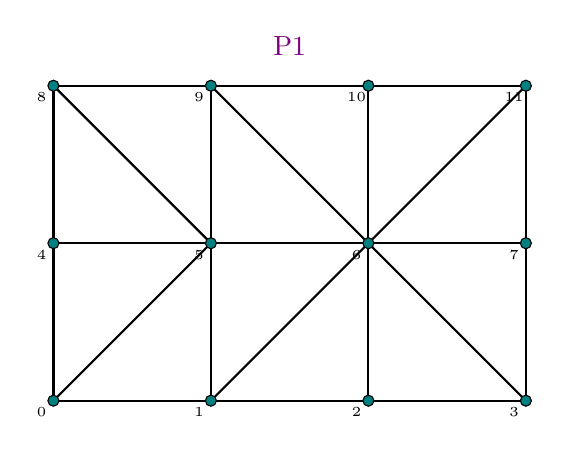
\begin{tikzpicture} 
\node[violet] at (3,4.5) {P1}; 
\draw[thick] (0,0) -- (6,0) -- (6,4) -- (0,4) -- cycle; 
\draw[thick] (0,2) -- (6,2) ; 
\draw[thick] (2,0) -- (2,4) ; 
\draw[thick] (4,0) -- (4,4) ; 
\draw[thick] (0,0) -- (2,2) -- (0,4) ; 
\draw[thick] (2,0) -- (4,2) -- (2,4) ; 
\draw[thick] (6,0) -- (4,2) -- (6,4) ; 
\draw[black,fill=teal] ( 0.000000 , 0.000000)     circle (2pt); 
\node[] at ( -0.150000, -0.150000 ) {\tiny 0 }; 
\draw[black,fill=teal] ( 2.000000 , 0.000000)     circle (2pt); 
\node[] at ( 1.850000, -0.150000 ) {\tiny 1 }; 
\draw[black,fill=teal] ( 4.000000 , 0.000000)     circle (2pt); 
\node[] at ( 3.850000, -0.150000 ) {\tiny 2 }; 
\draw[black,fill=teal] ( 6.000000 , 0.000000)     circle (2pt); 
\node[] at ( 5.850000, -0.150000 ) {\tiny 3 }; 
\draw[black,fill=teal] ( 0.000000 , 2.000000)     circle (2pt); 
\node[] at ( -0.150000, 1.850000 ) {\tiny 4 }; 
\draw[black,fill=teal] ( 2.000000 , 2.000000)     circle (2pt); 
\node[] at ( 1.850000, 1.850000 ) {\tiny 5 }; 
\draw[black,fill=teal] ( 4.000000 , 2.000000)     circle (2pt); 
\node[] at ( 3.850000, 1.850000 ) {\tiny 6 }; 
\draw[black,fill=teal] ( 6.000000 , 2.000000)     circle (2pt); 
\node[] at ( 5.850000, 1.850000 ) {\tiny 7 }; 
\draw[black,fill=teal] ( 0.000000 , 4.000000)     circle (2pt); 
\node[] at ( -0.150000, 3.850000 ) {\tiny 8 }; 
\draw[black,fill=teal] ( 2.000000 , 4.000000)     circle (2pt); 
\node[] at ( 1.850000, 3.850000 ) {\tiny 9 }; 
\draw[black,fill=teal] ( 4.000000 , 4.000000)     circle (2pt); 
\node[] at ( 3.850000, 3.850000 ) {\tiny 10 }; 
\draw[black,fill=teal] ( 6.000000 , 4.000000)     circle (2pt); 
\node[] at ( 5.850000, 3.850000 ) {\tiny 11 }; 
\end{tikzpicture} 
\end{center} 


\begin{tiny}
\verbatiminput{python_codes/fieldstone_120/spaces/iconV_elt1_P1.ascii}
\end{tiny}
\end{multicols}

%------------------
\begin{multicols}{2}
\begin{center} 
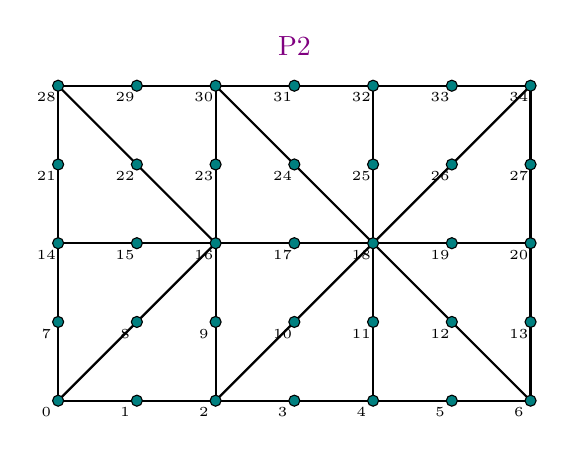
\begin{tikzpicture} 
\node[violet] at (3,4.5) {P2}; 
\draw[thick] (0,0) -- (6,0) -- (6,4) -- (0,4) -- cycle; 
\draw[thick] (0,2) -- (6,2) ; 
\draw[thick] (2,0) -- (2,4) ; 
\draw[thick] (4,0) -- (4,4) ; 
\draw[thick] (0,0) -- (2,2) -- (0,4) ; 
\draw[thick] (2,0) -- (4,2) -- (2,4) ; 
\draw[thick] (6,0) -- (4,2) -- (6,4) ; 
\draw[black,fill=teal] ( 0.000000 , 0.000000)     circle (2pt); 
\node[] at ( -0.150000, -0.150000 ) {\tiny 0 }; 
\draw[black,fill=teal] ( 1.000000 , 0.000000)     circle (2pt); 
\node[] at ( 0.850000, -0.150000 ) {\tiny 1 }; 
\draw[black,fill=teal] ( 2.000000 , 0.000000)     circle (2pt); 
\node[] at ( 1.850000, -0.150000 ) {\tiny 2 }; 
\draw[black,fill=teal] ( 3.000000 , 0.000000)     circle (2pt); 
\node[] at ( 2.850000, -0.150000 ) {\tiny 3 }; 
\draw[black,fill=teal] ( 4.000000 , 0.000000)     circle (2pt); 
\node[] at ( 3.850000, -0.150000 ) {\tiny 4 }; 
\draw[black,fill=teal] ( 5.000000 , 0.000000)     circle (2pt); 
\node[] at ( 4.850000, -0.150000 ) {\tiny 5 }; 
\draw[black,fill=teal] ( 6.000000 , 0.000000)     circle (2pt); 
\node[] at ( 5.850000, -0.150000 ) {\tiny 6 }; 
\draw[black,fill=teal] ( 0.000000 , 1.000000)     circle (2pt); 
\node[] at ( -0.150000, 0.850000 ) {\tiny 7 }; 
\draw[black,fill=teal] ( 1.000000 , 1.000000)     circle (2pt); 
\node[] at ( 0.850000, 0.850000 ) {\tiny 8 }; 
\draw[black,fill=teal] ( 2.000000 , 1.000000)     circle (2pt); 
\node[] at ( 1.850000, 0.850000 ) {\tiny 9 }; 
\draw[black,fill=teal] ( 3.000000 , 1.000000)     circle (2pt); 
\node[] at ( 2.850000, 0.850000 ) {\tiny 10 }; 
\draw[black,fill=teal] ( 4.000000 , 1.000000)     circle (2pt); 
\node[] at ( 3.850000, 0.850000 ) {\tiny 11 }; 
\draw[black,fill=teal] ( 5.000000 , 1.000000)     circle (2pt); 
\node[] at ( 4.850000, 0.850000 ) {\tiny 12 }; 
\draw[black,fill=teal] ( 6.000000 , 1.000000)     circle (2pt); 
\node[] at ( 5.850000, 0.850000 ) {\tiny 13 }; 
\draw[black,fill=teal] ( 0.000000 , 2.000000)     circle (2pt); 
\node[] at ( -0.150000, 1.850000 ) {\tiny 14 }; 
\draw[black,fill=teal] ( 1.000000 , 2.000000)     circle (2pt); 
\node[] at ( 0.850000, 1.850000 ) {\tiny 15 }; 
\draw[black,fill=teal] ( 2.000000 , 2.000000)     circle (2pt); 
\node[] at ( 1.850000, 1.850000 ) {\tiny 16 }; 
\draw[black,fill=teal] ( 3.000000 , 2.000000)     circle (2pt); 
\node[] at ( 2.850000, 1.850000 ) {\tiny 17 }; 
\draw[black,fill=teal] ( 4.000000 , 2.000000)     circle (2pt); 
\node[] at ( 3.850000, 1.850000 ) {\tiny 18 }; 
\draw[black,fill=teal] ( 5.000000 , 2.000000)     circle (2pt); 
\node[] at ( 4.850000, 1.850000 ) {\tiny 19 }; 
\draw[black,fill=teal] ( 6.000000 , 2.000000)     circle (2pt); 
\node[] at ( 5.850000, 1.850000 ) {\tiny 20 }; 
\draw[black,fill=teal] ( 0.000000 , 3.000000)     circle (2pt); 
\node[] at ( -0.150000, 2.850000 ) {\tiny 21 }; 
\draw[black,fill=teal] ( 1.000000 , 3.000000)     circle (2pt); 
\node[] at ( 0.850000, 2.850000 ) {\tiny 22 }; 
\draw[black,fill=teal] ( 2.000000 , 3.000000)     circle (2pt); 
\node[] at ( 1.850000, 2.850000 ) {\tiny 23 }; 
\draw[black,fill=teal] ( 3.000000 , 3.000000)     circle (2pt); 
\node[] at ( 2.850000, 2.850000 ) {\tiny 24 }; 
\draw[black,fill=teal] ( 4.000000 , 3.000000)     circle (2pt); 
\node[] at ( 3.850000, 2.850000 ) {\tiny 25 }; 
\draw[black,fill=teal] ( 5.000000 , 3.000000)     circle (2pt); 
\node[] at ( 4.850000, 2.850000 ) {\tiny 26 }; 
\draw[black,fill=teal] ( 6.000000 , 3.000000)     circle (2pt); 
\node[] at ( 5.850000, 2.850000 ) {\tiny 27 }; 
\draw[black,fill=teal] ( 0.000000 , 4.000000)     circle (2pt); 
\node[] at ( -0.150000, 3.850000 ) {\tiny 28 }; 
\draw[black,fill=teal] ( 1.000000 , 4.000000)     circle (2pt); 
\node[] at ( 0.850000, 3.850000 ) {\tiny 29 }; 
\draw[black,fill=teal] ( 2.000000 , 4.000000)     circle (2pt); 
\node[] at ( 1.850000, 3.850000 ) {\tiny 30 }; 
\draw[black,fill=teal] ( 3.000000 , 4.000000)     circle (2pt); 
\node[] at ( 2.850000, 3.850000 ) {\tiny 31 }; 
\draw[black,fill=teal] ( 4.000000 , 4.000000)     circle (2pt); 
\node[] at ( 3.850000, 3.850000 ) {\tiny 32 }; 
\draw[black,fill=teal] ( 5.000000 , 4.000000)     circle (2pt); 
\node[] at ( 4.850000, 3.850000 ) {\tiny 33 }; 
\draw[black,fill=teal] ( 6.000000 , 4.000000)     circle (2pt); 
\node[] at ( 5.850000, 3.850000 ) {\tiny 34 }; 
\end{tikzpicture} 
\end{center} 


\begin{tiny}
\verbatiminput{python_codes/fieldstone_120/spaces/iconV_elt1_P2.ascii}
\end{tiny}
\end{multicols}

%------------------
\begin{multicols}{2}
\begin{center} 
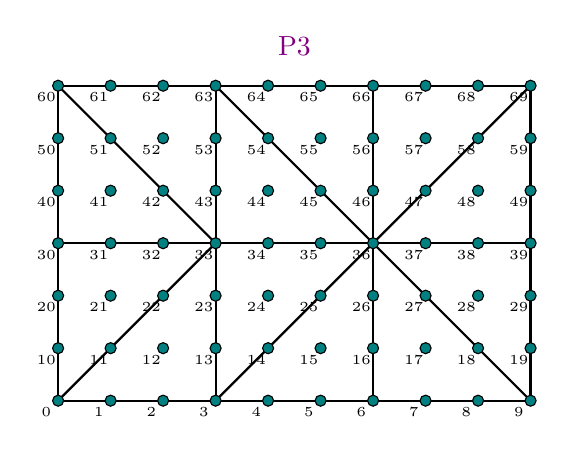
\begin{tikzpicture} 
\node[violet] at (3,4.5) {P3}; 
\draw[thick] (0,0) -- (6,0) -- (6,4) -- (0,4) -- cycle; 
\draw[thick] (0,2) -- (6,2) ; 
\draw[thick] (2,0) -- (2,4) ; 
\draw[thick] (4,0) -- (4,4) ; 
\draw[thick] (0,0) -- (2,2) -- (0,4) ; 
\draw[thick] (2,0) -- (4,2) -- (2,4) ; 
\draw[thick] (6,0) -- (4,2) -- (6,4) ; 
\draw[black,fill=teal] ( 0.000000 , 0.000000)     circle (2pt); 
\node[] at ( -0.150000, -0.150000 ) {\tiny 0 }; 
\draw[black,fill=teal] ( 0.666667 , 0.000000)     circle (2pt); 
\node[] at ( 0.516667, -0.150000 ) {\tiny 1 }; 
\draw[black,fill=teal] ( 1.333333 , 0.000000)     circle (2pt); 
\node[] at ( 1.183333, -0.150000 ) {\tiny 2 }; 
\draw[black,fill=teal] ( 2.000000 , 0.000000)     circle (2pt); 
\node[] at ( 1.850000, -0.150000 ) {\tiny 3 }; 
\draw[black,fill=teal] ( 2.666667 , 0.000000)     circle (2pt); 
\node[] at ( 2.516667, -0.150000 ) {\tiny 4 }; 
\draw[black,fill=teal] ( 3.333333 , 0.000000)     circle (2pt); 
\node[] at ( 3.183333, -0.150000 ) {\tiny 5 }; 
\draw[black,fill=teal] ( 4.000000 , 0.000000)     circle (2pt); 
\node[] at ( 3.850000, -0.150000 ) {\tiny 6 }; 
\draw[black,fill=teal] ( 4.666667 , 0.000000)     circle (2pt); 
\node[] at ( 4.516667, -0.150000 ) {\tiny 7 }; 
\draw[black,fill=teal] ( 5.333333 , 0.000000)     circle (2pt); 
\node[] at ( 5.183333, -0.150000 ) {\tiny 8 }; 
\draw[black,fill=teal] ( 6.000000 , 0.000000)     circle (2pt); 
\node[] at ( 5.850000, -0.150000 ) {\tiny 9 }; 
\draw[black,fill=teal] ( 0.000000 , 0.666667)     circle (2pt); 
\node[] at ( -0.150000, 0.516667 ) {\tiny 10 }; 
\draw[black,fill=teal] ( 0.666667 , 0.666667)     circle (2pt); 
\node[] at ( 0.516667, 0.516667 ) {\tiny 11 }; 
\draw[black,fill=teal] ( 1.333333 , 0.666667)     circle (2pt); 
\node[] at ( 1.183333, 0.516667 ) {\tiny 12 }; 
\draw[black,fill=teal] ( 2.000000 , 0.666667)     circle (2pt); 
\node[] at ( 1.850000, 0.516667 ) {\tiny 13 }; 
\draw[black,fill=teal] ( 2.666667 , 0.666667)     circle (2pt); 
\node[] at ( 2.516667, 0.516667 ) {\tiny 14 }; 
\draw[black,fill=teal] ( 3.333333 , 0.666667)     circle (2pt); 
\node[] at ( 3.183333, 0.516667 ) {\tiny 15 }; 
\draw[black,fill=teal] ( 4.000000 , 0.666667)     circle (2pt); 
\node[] at ( 3.850000, 0.516667 ) {\tiny 16 }; 
\draw[black,fill=teal] ( 4.666667 , 0.666667)     circle (2pt); 
\node[] at ( 4.516667, 0.516667 ) {\tiny 17 }; 
\draw[black,fill=teal] ( 5.333333 , 0.666667)     circle (2pt); 
\node[] at ( 5.183333, 0.516667 ) {\tiny 18 }; 
\draw[black,fill=teal] ( 6.000000 , 0.666667)     circle (2pt); 
\node[] at ( 5.850000, 0.516667 ) {\tiny 19 }; 
\draw[black,fill=teal] ( 0.000000 , 1.333333)     circle (2pt); 
\node[] at ( -0.150000, 1.183333 ) {\tiny 20 }; 
\draw[black,fill=teal] ( 0.666667 , 1.333333)     circle (2pt); 
\node[] at ( 0.516667, 1.183333 ) {\tiny 21 }; 
\draw[black,fill=teal] ( 1.333333 , 1.333333)     circle (2pt); 
\node[] at ( 1.183333, 1.183333 ) {\tiny 22 }; 
\draw[black,fill=teal] ( 2.000000 , 1.333333)     circle (2pt); 
\node[] at ( 1.850000, 1.183333 ) {\tiny 23 }; 
\draw[black,fill=teal] ( 2.666667 , 1.333333)     circle (2pt); 
\node[] at ( 2.516667, 1.183333 ) {\tiny 24 }; 
\draw[black,fill=teal] ( 3.333333 , 1.333333)     circle (2pt); 
\node[] at ( 3.183333, 1.183333 ) {\tiny 25 }; 
\draw[black,fill=teal] ( 4.000000 , 1.333333)     circle (2pt); 
\node[] at ( 3.850000, 1.183333 ) {\tiny 26 }; 
\draw[black,fill=teal] ( 4.666667 , 1.333333)     circle (2pt); 
\node[] at ( 4.516667, 1.183333 ) {\tiny 27 }; 
\draw[black,fill=teal] ( 5.333333 , 1.333333)     circle (2pt); 
\node[] at ( 5.183333, 1.183333 ) {\tiny 28 }; 
\draw[black,fill=teal] ( 6.000000 , 1.333333)     circle (2pt); 
\node[] at ( 5.850000, 1.183333 ) {\tiny 29 }; 
\draw[black,fill=teal] ( 0.000000 , 2.000000)     circle (2pt); 
\node[] at ( -0.150000, 1.850000 ) {\tiny 30 }; 
\draw[black,fill=teal] ( 0.666667 , 2.000000)     circle (2pt); 
\node[] at ( 0.516667, 1.850000 ) {\tiny 31 }; 
\draw[black,fill=teal] ( 1.333333 , 2.000000)     circle (2pt); 
\node[] at ( 1.183333, 1.850000 ) {\tiny 32 }; 
\draw[black,fill=teal] ( 2.000000 , 2.000000)     circle (2pt); 
\node[] at ( 1.850000, 1.850000 ) {\tiny 33 }; 
\draw[black,fill=teal] ( 2.666667 , 2.000000)     circle (2pt); 
\node[] at ( 2.516667, 1.850000 ) {\tiny 34 }; 
\draw[black,fill=teal] ( 3.333333 , 2.000000)     circle (2pt); 
\node[] at ( 3.183333, 1.850000 ) {\tiny 35 }; 
\draw[black,fill=teal] ( 4.000000 , 2.000000)     circle (2pt); 
\node[] at ( 3.850000, 1.850000 ) {\tiny 36 }; 
\draw[black,fill=teal] ( 4.666667 , 2.000000)     circle (2pt); 
\node[] at ( 4.516667, 1.850000 ) {\tiny 37 }; 
\draw[black,fill=teal] ( 5.333333 , 2.000000)     circle (2pt); 
\node[] at ( 5.183333, 1.850000 ) {\tiny 38 }; 
\draw[black,fill=teal] ( 6.000000 , 2.000000)     circle (2pt); 
\node[] at ( 5.850000, 1.850000 ) {\tiny 39 }; 
\draw[black,fill=teal] ( 0.000000 , 2.666667)     circle (2pt); 
\node[] at ( -0.150000, 2.516667 ) {\tiny 40 }; 
\draw[black,fill=teal] ( 0.666667 , 2.666667)     circle (2pt); 
\node[] at ( 0.516667, 2.516667 ) {\tiny 41 }; 
\draw[black,fill=teal] ( 1.333333 , 2.666667)     circle (2pt); 
\node[] at ( 1.183333, 2.516667 ) {\tiny 42 }; 
\draw[black,fill=teal] ( 2.000000 , 2.666667)     circle (2pt); 
\node[] at ( 1.850000, 2.516667 ) {\tiny 43 }; 
\draw[black,fill=teal] ( 2.666667 , 2.666667)     circle (2pt); 
\node[] at ( 2.516667, 2.516667 ) {\tiny 44 }; 
\draw[black,fill=teal] ( 3.333333 , 2.666667)     circle (2pt); 
\node[] at ( 3.183333, 2.516667 ) {\tiny 45 }; 
\draw[black,fill=teal] ( 4.000000 , 2.666667)     circle (2pt); 
\node[] at ( 3.850000, 2.516667 ) {\tiny 46 }; 
\draw[black,fill=teal] ( 4.666667 , 2.666667)     circle (2pt); 
\node[] at ( 4.516667, 2.516667 ) {\tiny 47 }; 
\draw[black,fill=teal] ( 5.333333 , 2.666667)     circle (2pt); 
\node[] at ( 5.183333, 2.516667 ) {\tiny 48 }; 
\draw[black,fill=teal] ( 6.000000 , 2.666667)     circle (2pt); 
\node[] at ( 5.850000, 2.516667 ) {\tiny 49 }; 
\draw[black,fill=teal] ( 0.000000 , 3.333333)     circle (2pt); 
\node[] at ( -0.150000, 3.183333 ) {\tiny 50 }; 
\draw[black,fill=teal] ( 0.666667 , 3.333333)     circle (2pt); 
\node[] at ( 0.516667, 3.183333 ) {\tiny 51 }; 
\draw[black,fill=teal] ( 1.333333 , 3.333333)     circle (2pt); 
\node[] at ( 1.183333, 3.183333 ) {\tiny 52 }; 
\draw[black,fill=teal] ( 2.000000 , 3.333333)     circle (2pt); 
\node[] at ( 1.850000, 3.183333 ) {\tiny 53 }; 
\draw[black,fill=teal] ( 2.666667 , 3.333333)     circle (2pt); 
\node[] at ( 2.516667, 3.183333 ) {\tiny 54 }; 
\draw[black,fill=teal] ( 3.333333 , 3.333333)     circle (2pt); 
\node[] at ( 3.183333, 3.183333 ) {\tiny 55 }; 
\draw[black,fill=teal] ( 4.000000 , 3.333333)     circle (2pt); 
\node[] at ( 3.850000, 3.183333 ) {\tiny 56 }; 
\draw[black,fill=teal] ( 4.666667 , 3.333333)     circle (2pt); 
\node[] at ( 4.516667, 3.183333 ) {\tiny 57 }; 
\draw[black,fill=teal] ( 5.333333 , 3.333333)     circle (2pt); 
\node[] at ( 5.183333, 3.183333 ) {\tiny 58 }; 
\draw[black,fill=teal] ( 6.000000 , 3.333333)     circle (2pt); 
\node[] at ( 5.850000, 3.183333 ) {\tiny 59 }; 
\draw[black,fill=teal] ( 0.000000 , 4.000000)     circle (2pt); 
\node[] at ( -0.150000, 3.850000 ) {\tiny 60 }; 
\draw[black,fill=teal] ( 0.666667 , 4.000000)     circle (2pt); 
\node[] at ( 0.516667, 3.850000 ) {\tiny 61 }; 
\draw[black,fill=teal] ( 1.333333 , 4.000000)     circle (2pt); 
\node[] at ( 1.183333, 3.850000 ) {\tiny 62 }; 
\draw[black,fill=teal] ( 2.000000 , 4.000000)     circle (2pt); 
\node[] at ( 1.850000, 3.850000 ) {\tiny 63 }; 
\draw[black,fill=teal] ( 2.666667 , 4.000000)     circle (2pt); 
\node[] at ( 2.516667, 3.850000 ) {\tiny 64 }; 
\draw[black,fill=teal] ( 3.333333 , 4.000000)     circle (2pt); 
\node[] at ( 3.183333, 3.850000 ) {\tiny 65 }; 
\draw[black,fill=teal] ( 4.000000 , 4.000000)     circle (2pt); 
\node[] at ( 3.850000, 3.850000 ) {\tiny 66 }; 
\draw[black,fill=teal] ( 4.666667 , 4.000000)     circle (2pt); 
\node[] at ( 4.516667, 3.850000 ) {\tiny 67 }; 
\draw[black,fill=teal] ( 5.333333 , 4.000000)     circle (2pt); 
\node[] at ( 5.183333, 3.850000 ) {\tiny 68 }; 
\draw[black,fill=teal] ( 6.000000 , 4.000000)     circle (2pt); 
\node[] at ( 5.850000, 3.850000 ) {\tiny 69 }; 
\end{tikzpicture} 
\end{center} 


\begin{tiny}
\verbatiminput{python_codes/fieldstone_120/spaces/iconV_elt1_P3.ascii}
\end{tiny}
\end{multicols}

\newpage
%------------------
\begin{multicols}{2}
\begin{center} 
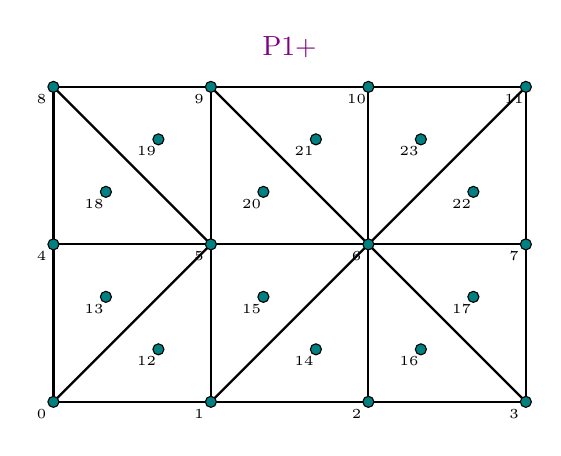
\begin{tikzpicture} 
\node[violet] at (3,4.5) {P1+}; 
\draw[thick] (0,0) -- (6,0) -- (6,4) -- (0,4) -- cycle; 
\draw[thick] (0,2) -- (6,2) ; 
\draw[thick] (2,0) -- (2,4) ; 
\draw[thick] (4,0) -- (4,4) ; 
\draw[thick] (0,0) -- (2,2) -- (0,4) ; 
\draw[thick] (2,0) -- (4,2) -- (2,4) ; 
\draw[thick] (6,0) -- (4,2) -- (6,4) ; 
\draw[black,fill=teal] ( 0.000000 , 0.000000)     circle (2pt); 
\node[] at ( -0.150000, -0.150000 ) {\tiny 0 }; 
\draw[black,fill=teal] ( 2.000000 , 0.000000)     circle (2pt); 
\node[] at ( 1.850000, -0.150000 ) {\tiny 1 }; 
\draw[black,fill=teal] ( 4.000000 , 0.000000)     circle (2pt); 
\node[] at ( 3.850000, -0.150000 ) {\tiny 2 }; 
\draw[black,fill=teal] ( 6.000000 , 0.000000)     circle (2pt); 
\node[] at ( 5.850000, -0.150000 ) {\tiny 3 }; 
\draw[black,fill=teal] ( 0.000000 , 2.000000)     circle (2pt); 
\node[] at ( -0.150000, 1.850000 ) {\tiny 4 }; 
\draw[black,fill=teal] ( 2.000000 , 2.000000)     circle (2pt); 
\node[] at ( 1.850000, 1.850000 ) {\tiny 5 }; 
\draw[black,fill=teal] ( 4.000000 , 2.000000)     circle (2pt); 
\node[] at ( 3.850000, 1.850000 ) {\tiny 6 }; 
\draw[black,fill=teal] ( 6.000000 , 2.000000)     circle (2pt); 
\node[] at ( 5.850000, 1.850000 ) {\tiny 7 }; 
\draw[black,fill=teal] ( 0.000000 , 4.000000)     circle (2pt); 
\node[] at ( -0.150000, 3.850000 ) {\tiny 8 }; 
\draw[black,fill=teal] ( 2.000000 , 4.000000)     circle (2pt); 
\node[] at ( 1.850000, 3.850000 ) {\tiny 9 }; 
\draw[black,fill=teal] ( 4.000000 , 4.000000)     circle (2pt); 
\node[] at ( 3.850000, 3.850000 ) {\tiny 10 }; 
\draw[black,fill=teal] ( 6.000000 , 4.000000)     circle (2pt); 
\node[] at ( 5.850000, 3.850000 ) {\tiny 11 }; 
\draw[black,fill=teal] ( 1.333333 , 0.666667)     circle (2pt); 
\node[] at ( 1.183333, 0.516667 ) {\tiny 12 }; 
\draw[black,fill=teal] ( 0.666667 , 1.333333)     circle (2pt); 
\node[] at ( 0.516667, 1.183333 ) {\tiny 13 }; 
\draw[black,fill=teal] ( 3.333333 , 0.666667)     circle (2pt); 
\node[] at ( 3.183333, 0.516667 ) {\tiny 14 }; 
\draw[black,fill=teal] ( 2.666667 , 1.333333)     circle (2pt); 
\node[] at ( 2.516667, 1.183333 ) {\tiny 15 }; 
\draw[black,fill=teal] ( 4.666667 , 0.666667)     circle (2pt); 
\node[] at ( 4.516667, 0.516667 ) {\tiny 16 }; 
\draw[black,fill=teal] ( 5.333333 , 1.333333)     circle (2pt); 
\node[] at ( 5.183333, 1.183333 ) {\tiny 17 }; 
\draw[black,fill=teal] ( 0.666667 , 2.666667)     circle (2pt); 
\node[] at ( 0.516667, 2.516667 ) {\tiny 18 }; 
\draw[black,fill=teal] ( 1.333333 , 3.333333)     circle (2pt); 
\node[] at ( 1.183333, 3.183333 ) {\tiny 19 }; 
\draw[black,fill=teal] ( 2.666667 , 2.666667)     circle (2pt); 
\node[] at ( 2.516667, 2.516667 ) {\tiny 20 }; 
\draw[black,fill=teal] ( 3.333333 , 3.333333)     circle (2pt); 
\node[] at ( 3.183333, 3.183333 ) {\tiny 21 }; 
\draw[black,fill=teal] ( 5.333333 , 2.666667)     circle (2pt); 
\node[] at ( 5.183333, 2.516667 ) {\tiny 22 }; 
\draw[black,fill=teal] ( 4.666667 , 3.333333)     circle (2pt); 
\node[] at ( 4.516667, 3.183333 ) {\tiny 23 }; 
\end{tikzpicture} 
\end{center} 


\begin{tiny}
\verbatiminput{python_codes/fieldstone_120/spaces/iconV_elt1_P1+.ascii}
\end{tiny}
\end{multicols}

%------------------
\begin{multicols}{2}
\begin{center} 
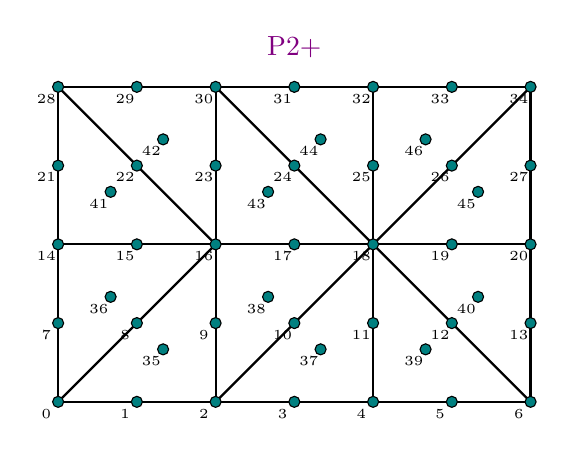
\begin{tikzpicture} 
\node[violet] at (3,4.5) {P2+}; 
\draw[thick] (0,0) -- (6,0) -- (6,4) -- (0,4) -- cycle; 
\draw[thick] (0,2) -- (6,2) ; 
\draw[thick] (2,0) -- (2,4) ; 
\draw[thick] (4,0) -- (4,4) ; 
\draw[thick] (0,0) -- (2,2) -- (0,4) ; 
\draw[thick] (2,0) -- (4,2) -- (2,4) ; 
\draw[thick] (6,0) -- (4,2) -- (6,4) ; 
\draw[black,fill=teal] ( 0.000000 , 0.000000)     circle (2pt); 
\node[] at ( -0.150000, -0.150000 ) {\tiny 0 }; 
\draw[black,fill=teal] ( 1.000000 , 0.000000)     circle (2pt); 
\node[] at ( 0.850000, -0.150000 ) {\tiny 1 }; 
\draw[black,fill=teal] ( 2.000000 , 0.000000)     circle (2pt); 
\node[] at ( 1.850000, -0.150000 ) {\tiny 2 }; 
\draw[black,fill=teal] ( 3.000000 , 0.000000)     circle (2pt); 
\node[] at ( 2.850000, -0.150000 ) {\tiny 3 }; 
\draw[black,fill=teal] ( 4.000000 , 0.000000)     circle (2pt); 
\node[] at ( 3.850000, -0.150000 ) {\tiny 4 }; 
\draw[black,fill=teal] ( 5.000000 , 0.000000)     circle (2pt); 
\node[] at ( 4.850000, -0.150000 ) {\tiny 5 }; 
\draw[black,fill=teal] ( 6.000000 , 0.000000)     circle (2pt); 
\node[] at ( 5.850000, -0.150000 ) {\tiny 6 }; 
\draw[black,fill=teal] ( 0.000000 , 1.000000)     circle (2pt); 
\node[] at ( -0.150000, 0.850000 ) {\tiny 7 }; 
\draw[black,fill=teal] ( 1.000000 , 1.000000)     circle (2pt); 
\node[] at ( 0.850000, 0.850000 ) {\tiny 8 }; 
\draw[black,fill=teal] ( 2.000000 , 1.000000)     circle (2pt); 
\node[] at ( 1.850000, 0.850000 ) {\tiny 9 }; 
\draw[black,fill=teal] ( 3.000000 , 1.000000)     circle (2pt); 
\node[] at ( 2.850000, 0.850000 ) {\tiny 10 }; 
\draw[black,fill=teal] ( 4.000000 , 1.000000)     circle (2pt); 
\node[] at ( 3.850000, 0.850000 ) {\tiny 11 }; 
\draw[black,fill=teal] ( 5.000000 , 1.000000)     circle (2pt); 
\node[] at ( 4.850000, 0.850000 ) {\tiny 12 }; 
\draw[black,fill=teal] ( 6.000000 , 1.000000)     circle (2pt); 
\node[] at ( 5.850000, 0.850000 ) {\tiny 13 }; 
\draw[black,fill=teal] ( 0.000000 , 2.000000)     circle (2pt); 
\node[] at ( -0.150000, 1.850000 ) {\tiny 14 }; 
\draw[black,fill=teal] ( 1.000000 , 2.000000)     circle (2pt); 
\node[] at ( 0.850000, 1.850000 ) {\tiny 15 }; 
\draw[black,fill=teal] ( 2.000000 , 2.000000)     circle (2pt); 
\node[] at ( 1.850000, 1.850000 ) {\tiny 16 }; 
\draw[black,fill=teal] ( 3.000000 , 2.000000)     circle (2pt); 
\node[] at ( 2.850000, 1.850000 ) {\tiny 17 }; 
\draw[black,fill=teal] ( 4.000000 , 2.000000)     circle (2pt); 
\node[] at ( 3.850000, 1.850000 ) {\tiny 18 }; 
\draw[black,fill=teal] ( 5.000000 , 2.000000)     circle (2pt); 
\node[] at ( 4.850000, 1.850000 ) {\tiny 19 }; 
\draw[black,fill=teal] ( 6.000000 , 2.000000)     circle (2pt); 
\node[] at ( 5.850000, 1.850000 ) {\tiny 20 }; 
\draw[black,fill=teal] ( 0.000000 , 3.000000)     circle (2pt); 
\node[] at ( -0.150000, 2.850000 ) {\tiny 21 }; 
\draw[black,fill=teal] ( 1.000000 , 3.000000)     circle (2pt); 
\node[] at ( 0.850000, 2.850000 ) {\tiny 22 }; 
\draw[black,fill=teal] ( 2.000000 , 3.000000)     circle (2pt); 
\node[] at ( 1.850000, 2.850000 ) {\tiny 23 }; 
\draw[black,fill=teal] ( 3.000000 , 3.000000)     circle (2pt); 
\node[] at ( 2.850000, 2.850000 ) {\tiny 24 }; 
\draw[black,fill=teal] ( 4.000000 , 3.000000)     circle (2pt); 
\node[] at ( 3.850000, 2.850000 ) {\tiny 25 }; 
\draw[black,fill=teal] ( 5.000000 , 3.000000)     circle (2pt); 
\node[] at ( 4.850000, 2.850000 ) {\tiny 26 }; 
\draw[black,fill=teal] ( 6.000000 , 3.000000)     circle (2pt); 
\node[] at ( 5.850000, 2.850000 ) {\tiny 27 }; 
\draw[black,fill=teal] ( 0.000000 , 4.000000)     circle (2pt); 
\node[] at ( -0.150000, 3.850000 ) {\tiny 28 }; 
\draw[black,fill=teal] ( 1.000000 , 4.000000)     circle (2pt); 
\node[] at ( 0.850000, 3.850000 ) {\tiny 29 }; 
\draw[black,fill=teal] ( 2.000000 , 4.000000)     circle (2pt); 
\node[] at ( 1.850000, 3.850000 ) {\tiny 30 }; 
\draw[black,fill=teal] ( 3.000000 , 4.000000)     circle (2pt); 
\node[] at ( 2.850000, 3.850000 ) {\tiny 31 }; 
\draw[black,fill=teal] ( 4.000000 , 4.000000)     circle (2pt); 
\node[] at ( 3.850000, 3.850000 ) {\tiny 32 }; 
\draw[black,fill=teal] ( 5.000000 , 4.000000)     circle (2pt); 
\node[] at ( 4.850000, 3.850000 ) {\tiny 33 }; 
\draw[black,fill=teal] ( 6.000000 , 4.000000)     circle (2pt); 
\node[] at ( 5.850000, 3.850000 ) {\tiny 34 }; 
\draw[black,fill=teal] ( 1.333333 , 0.666667)     circle (2pt); 
\node[] at ( 1.183333, 0.516667 ) {\tiny 35 }; 
\draw[black,fill=teal] ( 0.666667 , 1.333333)     circle (2pt); 
\node[] at ( 0.516667, 1.183333 ) {\tiny 36 }; 
\draw[black,fill=teal] ( 3.333333 , 0.666667)     circle (2pt); 
\node[] at ( 3.183333, 0.516667 ) {\tiny 37 }; 
\draw[black,fill=teal] ( 2.666667 , 1.333333)     circle (2pt); 
\node[] at ( 2.516667, 1.183333 ) {\tiny 38 }; 
\draw[black,fill=teal] ( 4.666667 , 0.666667)     circle (2pt); 
\node[] at ( 4.516667, 0.516667 ) {\tiny 39 }; 
\draw[black,fill=teal] ( 5.333333 , 1.333333)     circle (2pt); 
\node[] at ( 5.183333, 1.183333 ) {\tiny 40 }; 
\draw[black,fill=teal] ( 0.666667 , 2.666667)     circle (2pt); 
\node[] at ( 0.516667, 2.516667 ) {\tiny 41 }; 
\draw[black,fill=teal] ( 1.333333 , 3.333333)     circle (2pt); 
\node[] at ( 1.183333, 3.183333 ) {\tiny 42 }; 
\draw[black,fill=teal] ( 2.666667 , 2.666667)     circle (2pt); 
\node[] at ( 2.516667, 2.516667 ) {\tiny 43 }; 
\draw[black,fill=teal] ( 3.333333 , 3.333333)     circle (2pt); 
\node[] at ( 3.183333, 3.183333 ) {\tiny 44 }; 
\draw[black,fill=teal] ( 5.333333 , 2.666667)     circle (2pt); 
\node[] at ( 5.183333, 2.516667 ) {\tiny 45 }; 
\draw[black,fill=teal] ( 4.666667 , 3.333333)     circle (2pt); 
\node[] at ( 4.516667, 3.183333 ) {\tiny 46 }; 
\end{tikzpicture} 
\end{center} 


\begin{tiny}
\verbatiminput{python_codes/fieldstone_120/spaces/iconV_elt1_P2+.ascii}
\end{tiny}
\end{multicols}

%------------------
\begin{multicols}{2}
\begin{center} 
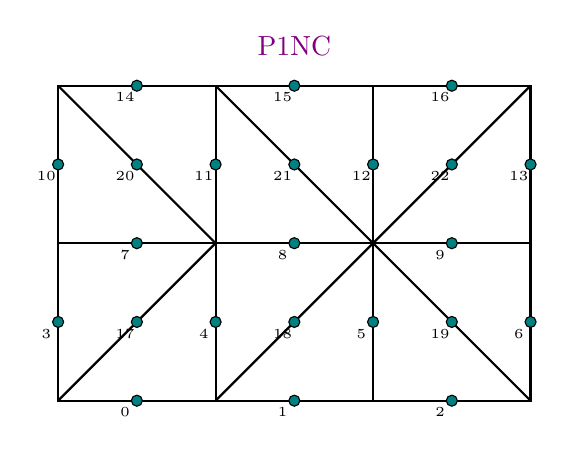
\begin{tikzpicture} 
\node[violet] at (3,4.5) {P1NC}; 
\draw[thick] (0,0) -- (6,0) -- (6,4) -- (0,4) -- cycle; 
\draw[thick] (0,2) -- (6,2) ; 
\draw[thick] (2,0) -- (2,4) ; 
\draw[thick] (4,0) -- (4,4) ; 
\draw[thick] (0,0) -- (2,2) -- (0,4) ; 
\draw[thick] (2,0) -- (4,2) -- (2,4) ; 
\draw[thick] (6,0) -- (4,2) -- (6,4) ; 
\draw[black,fill=teal] ( 1.000000 , 0.000000)     circle (2pt); 
\node[] at ( 0.850000, -0.150000 ) {\tiny 0 }; 
\draw[black,fill=teal] ( 3.000000 , 0.000000)     circle (2pt); 
\node[] at ( 2.850000, -0.150000 ) {\tiny 1 }; 
\draw[black,fill=teal] ( 5.000000 , 0.000000)     circle (2pt); 
\node[] at ( 4.850000, -0.150000 ) {\tiny 2 }; 
\draw[black,fill=teal] ( 0.000000 , 1.000000)     circle (2pt); 
\node[] at ( -0.150000, 0.850000 ) {\tiny 3 }; 
\draw[black,fill=teal] ( 2.000000 , 1.000000)     circle (2pt); 
\node[] at ( 1.850000, 0.850000 ) {\tiny 4 }; 
\draw[black,fill=teal] ( 4.000000 , 1.000000)     circle (2pt); 
\node[] at ( 3.850000, 0.850000 ) {\tiny 5 }; 
\draw[black,fill=teal] ( 6.000000 , 1.000000)     circle (2pt); 
\node[] at ( 5.850000, 0.850000 ) {\tiny 6 }; 
\draw[black,fill=teal] ( 1.000000 , 2.000000)     circle (2pt); 
\node[] at ( 0.850000, 1.850000 ) {\tiny 7 }; 
\draw[black,fill=teal] ( 3.000000 , 2.000000)     circle (2pt); 
\node[] at ( 2.850000, 1.850000 ) {\tiny 8 }; 
\draw[black,fill=teal] ( 5.000000 , 2.000000)     circle (2pt); 
\node[] at ( 4.850000, 1.850000 ) {\tiny 9 }; 
\draw[black,fill=teal] ( 0.000000 , 3.000000)     circle (2pt); 
\node[] at ( -0.150000, 2.850000 ) {\tiny 10 }; 
\draw[black,fill=teal] ( 2.000000 , 3.000000)     circle (2pt); 
\node[] at ( 1.850000, 2.850000 ) {\tiny 11 }; 
\draw[black,fill=teal] ( 4.000000 , 3.000000)     circle (2pt); 
\node[] at ( 3.850000, 2.850000 ) {\tiny 12 }; 
\draw[black,fill=teal] ( 6.000000 , 3.000000)     circle (2pt); 
\node[] at ( 5.850000, 2.850000 ) {\tiny 13 }; 
\draw[black,fill=teal] ( 1.000000 , 4.000000)     circle (2pt); 
\node[] at ( 0.850000, 3.850000 ) {\tiny 14 }; 
\draw[black,fill=teal] ( 3.000000 , 4.000000)     circle (2pt); 
\node[] at ( 2.850000, 3.850000 ) {\tiny 15 }; 
\draw[black,fill=teal] ( 5.000000 , 4.000000)     circle (2pt); 
\node[] at ( 4.850000, 3.850000 ) {\tiny 16 }; 
\draw[black,fill=teal] ( 1.000000 , 1.000000)     circle (2pt); 
\node[] at ( 0.850000, 0.850000 ) {\tiny 17 }; 
\draw[black,fill=teal] ( 3.000000 , 1.000000)     circle (2pt); 
\node[] at ( 2.850000, 0.850000 ) {\tiny 18 }; 
\draw[black,fill=teal] ( 5.000000 , 1.000000)     circle (2pt); 
\node[] at ( 4.850000, 0.850000 ) {\tiny 19 }; 
\draw[black,fill=teal] ( 1.000000 , 3.000000)     circle (2pt); 
\node[] at ( 0.850000, 2.850000 ) {\tiny 20 }; 
\draw[black,fill=teal] ( 3.000000 , 3.000000)     circle (2pt); 
\node[] at ( 2.850000, 2.850000 ) {\tiny 21 }; 
\draw[black,fill=teal] ( 5.000000 , 3.000000)     circle (2pt); 
\node[] at ( 4.850000, 2.850000 ) {\tiny 22 }; 
\end{tikzpicture} 
\end{center} 


\begin{tiny}
\verbatiminput{python_codes/fieldstone_120/spaces/iconV_elt1_P1NC.ascii}
\end{tiny}
\end{multicols}

\newpage
%------------------
\begin{multicols}{2}
\begin{center} 
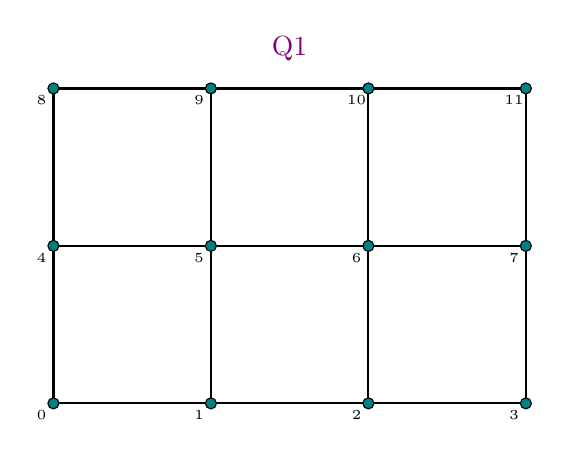
\begin{tikzpicture} 
\node[violet] at (3,4.5) {Q1}; 
\draw[thick] (0,0) -- (6,0) -- (6,4) -- (0,4) -- cycle; 
\draw[thick] (0,2) -- (6,2) ; 
\draw[thick] (2,0) -- (2,4) ; 
\draw[thick] (4,0) -- (4,4) ; 
\draw[black,fill=teal] ( 0.000000 , 0.000000)     circle (2pt); 
\node[] at ( -0.150000, -0.150000 ) {\tiny 0 }; 
\draw[black,fill=teal] ( 2.000000 , 0.000000)     circle (2pt); 
\node[] at ( 1.850000, -0.150000 ) {\tiny 1 }; 
\draw[black,fill=teal] ( 4.000000 , 0.000000)     circle (2pt); 
\node[] at ( 3.850000, -0.150000 ) {\tiny 2 }; 
\draw[black,fill=teal] ( 6.000000 , 0.000000)     circle (2pt); 
\node[] at ( 5.850000, -0.150000 ) {\tiny 3 }; 
\draw[black,fill=teal] ( 0.000000 , 2.000000)     circle (2pt); 
\node[] at ( -0.150000, 1.850000 ) {\tiny 4 }; 
\draw[black,fill=teal] ( 2.000000 , 2.000000)     circle (2pt); 
\node[] at ( 1.850000, 1.850000 ) {\tiny 5 }; 
\draw[black,fill=teal] ( 4.000000 , 2.000000)     circle (2pt); 
\node[] at ( 3.850000, 1.850000 ) {\tiny 6 }; 
\draw[black,fill=teal] ( 6.000000 , 2.000000)     circle (2pt); 
\node[] at ( 5.850000, 1.850000 ) {\tiny 7 }; 
\draw[black,fill=teal] ( 0.000000 , 4.000000)     circle (2pt); 
\node[] at ( -0.150000, 3.850000 ) {\tiny 8 }; 
\draw[black,fill=teal] ( 2.000000 , 4.000000)     circle (2pt); 
\node[] at ( 1.850000, 3.850000 ) {\tiny 9 }; 
\draw[black,fill=teal] ( 4.000000 , 4.000000)     circle (2pt); 
\node[] at ( 3.850000, 3.850000 ) {\tiny 10 }; 
\draw[black,fill=teal] ( 6.000000 , 4.000000)     circle (2pt); 
\node[] at ( 5.850000, 3.850000 ) {\tiny 11 }; 
\end{tikzpicture} 
\end{center} 


\begin{tiny}
\verbatiminput{python_codes/fieldstone_120/spaces/iconV_elt1_Q1.ascii}
\end{tiny}
\end{multicols}

%------------------
\begin{multicols}{2}
\begin{center} 
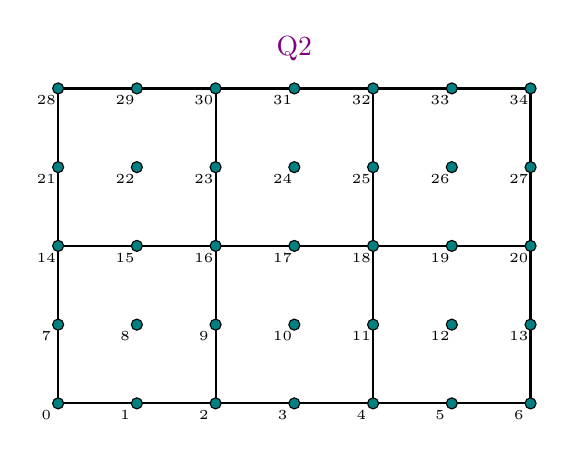
\begin{tikzpicture} 
\node[violet] at (3,4.5) {Q2}; 
\draw[thick] (0,0) -- (6,0) -- (6,4) -- (0,4) -- cycle; 
\draw[thick] (0,2) -- (6,2) ; 
\draw[thick] (2,0) -- (2,4) ; 
\draw[thick] (4,0) -- (4,4) ; 
\draw[black,fill=teal] ( 0.000000 , 0.000000)     circle (2pt); 
\node[] at ( -0.150000, -0.150000 ) {\tiny 0 }; 
\draw[black,fill=teal] ( 1.000000 , 0.000000)     circle (2pt); 
\node[] at ( 0.850000, -0.150000 ) {\tiny 1 }; 
\draw[black,fill=teal] ( 2.000000 , 0.000000)     circle (2pt); 
\node[] at ( 1.850000, -0.150000 ) {\tiny 2 }; 
\draw[black,fill=teal] ( 3.000000 , 0.000000)     circle (2pt); 
\node[] at ( 2.850000, -0.150000 ) {\tiny 3 }; 
\draw[black,fill=teal] ( 4.000000 , 0.000000)     circle (2pt); 
\node[] at ( 3.850000, -0.150000 ) {\tiny 4 }; 
\draw[black,fill=teal] ( 5.000000 , 0.000000)     circle (2pt); 
\node[] at ( 4.850000, -0.150000 ) {\tiny 5 }; 
\draw[black,fill=teal] ( 6.000000 , 0.000000)     circle (2pt); 
\node[] at ( 5.850000, -0.150000 ) {\tiny 6 }; 
\draw[black,fill=teal] ( 0.000000 , 1.000000)     circle (2pt); 
\node[] at ( -0.150000, 0.850000 ) {\tiny 7 }; 
\draw[black,fill=teal] ( 1.000000 , 1.000000)     circle (2pt); 
\node[] at ( 0.850000, 0.850000 ) {\tiny 8 }; 
\draw[black,fill=teal] ( 2.000000 , 1.000000)     circle (2pt); 
\node[] at ( 1.850000, 0.850000 ) {\tiny 9 }; 
\draw[black,fill=teal] ( 3.000000 , 1.000000)     circle (2pt); 
\node[] at ( 2.850000, 0.850000 ) {\tiny 10 }; 
\draw[black,fill=teal] ( 4.000000 , 1.000000)     circle (2pt); 
\node[] at ( 3.850000, 0.850000 ) {\tiny 11 }; 
\draw[black,fill=teal] ( 5.000000 , 1.000000)     circle (2pt); 
\node[] at ( 4.850000, 0.850000 ) {\tiny 12 }; 
\draw[black,fill=teal] ( 6.000000 , 1.000000)     circle (2pt); 
\node[] at ( 5.850000, 0.850000 ) {\tiny 13 }; 
\draw[black,fill=teal] ( 0.000000 , 2.000000)     circle (2pt); 
\node[] at ( -0.150000, 1.850000 ) {\tiny 14 }; 
\draw[black,fill=teal] ( 1.000000 , 2.000000)     circle (2pt); 
\node[] at ( 0.850000, 1.850000 ) {\tiny 15 }; 
\draw[black,fill=teal] ( 2.000000 , 2.000000)     circle (2pt); 
\node[] at ( 1.850000, 1.850000 ) {\tiny 16 }; 
\draw[black,fill=teal] ( 3.000000 , 2.000000)     circle (2pt); 
\node[] at ( 2.850000, 1.850000 ) {\tiny 17 }; 
\draw[black,fill=teal] ( 4.000000 , 2.000000)     circle (2pt); 
\node[] at ( 3.850000, 1.850000 ) {\tiny 18 }; 
\draw[black,fill=teal] ( 5.000000 , 2.000000)     circle (2pt); 
\node[] at ( 4.850000, 1.850000 ) {\tiny 19 }; 
\draw[black,fill=teal] ( 6.000000 , 2.000000)     circle (2pt); 
\node[] at ( 5.850000, 1.850000 ) {\tiny 20 }; 
\draw[black,fill=teal] ( 0.000000 , 3.000000)     circle (2pt); 
\node[] at ( -0.150000, 2.850000 ) {\tiny 21 }; 
\draw[black,fill=teal] ( 1.000000 , 3.000000)     circle (2pt); 
\node[] at ( 0.850000, 2.850000 ) {\tiny 22 }; 
\draw[black,fill=teal] ( 2.000000 , 3.000000)     circle (2pt); 
\node[] at ( 1.850000, 2.850000 ) {\tiny 23 }; 
\draw[black,fill=teal] ( 3.000000 , 3.000000)     circle (2pt); 
\node[] at ( 2.850000, 2.850000 ) {\tiny 24 }; 
\draw[black,fill=teal] ( 4.000000 , 3.000000)     circle (2pt); 
\node[] at ( 3.850000, 2.850000 ) {\tiny 25 }; 
\draw[black,fill=teal] ( 5.000000 , 3.000000)     circle (2pt); 
\node[] at ( 4.850000, 2.850000 ) {\tiny 26 }; 
\draw[black,fill=teal] ( 6.000000 , 3.000000)     circle (2pt); 
\node[] at ( 5.850000, 2.850000 ) {\tiny 27 }; 
\draw[black,fill=teal] ( 0.000000 , 4.000000)     circle (2pt); 
\node[] at ( -0.150000, 3.850000 ) {\tiny 28 }; 
\draw[black,fill=teal] ( 1.000000 , 4.000000)     circle (2pt); 
\node[] at ( 0.850000, 3.850000 ) {\tiny 29 }; 
\draw[black,fill=teal] ( 2.000000 , 4.000000)     circle (2pt); 
\node[] at ( 1.850000, 3.850000 ) {\tiny 30 }; 
\draw[black,fill=teal] ( 3.000000 , 4.000000)     circle (2pt); 
\node[] at ( 2.850000, 3.850000 ) {\tiny 31 }; 
\draw[black,fill=teal] ( 4.000000 , 4.000000)     circle (2pt); 
\node[] at ( 3.850000, 3.850000 ) {\tiny 32 }; 
\draw[black,fill=teal] ( 5.000000 , 4.000000)     circle (2pt); 
\node[] at ( 4.850000, 3.850000 ) {\tiny 33 }; 
\draw[black,fill=teal] ( 6.000000 , 4.000000)     circle (2pt); 
\node[] at ( 5.850000, 3.850000 ) {\tiny 34 }; 
\end{tikzpicture} 
\end{center} 


\begin{tiny}
\verbatiminput{python_codes/fieldstone_120/spaces/iconV_elt1_Q2.ascii}
\end{tiny}
\end{multicols}

%------------------
\begin{multicols}{2}
\begin{center} 
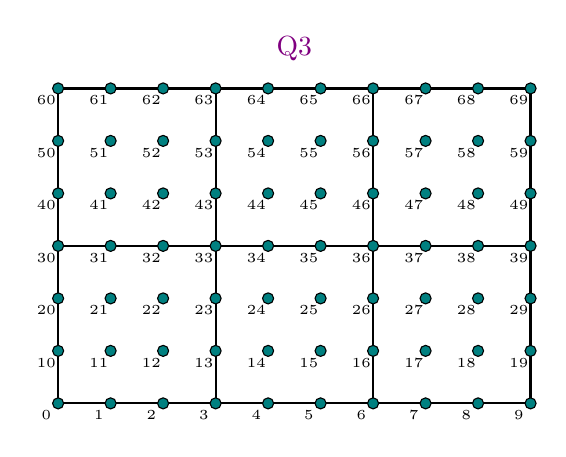
\begin{tikzpicture} 
\node[violet] at (3,4.5) {Q3}; 
\draw[thick] (0,0) -- (6,0) -- (6,4) -- (0,4) -- cycle; 
\draw[thick] (0,2) -- (6,2) ; 
\draw[thick] (2,0) -- (2,4) ; 
\draw[thick] (4,0) -- (4,4) ; 
\draw[black,fill=teal] ( 0.000000 , 0.000000)     circle (2pt); 
\node[] at ( -0.150000, -0.150000 ) {\tiny 0 }; 
\draw[black,fill=teal] ( 0.666667 , 0.000000)     circle (2pt); 
\node[] at ( 0.516667, -0.150000 ) {\tiny 1 }; 
\draw[black,fill=teal] ( 1.333333 , 0.000000)     circle (2pt); 
\node[] at ( 1.183333, -0.150000 ) {\tiny 2 }; 
\draw[black,fill=teal] ( 2.000000 , 0.000000)     circle (2pt); 
\node[] at ( 1.850000, -0.150000 ) {\tiny 3 }; 
\draw[black,fill=teal] ( 2.666667 , 0.000000)     circle (2pt); 
\node[] at ( 2.516667, -0.150000 ) {\tiny 4 }; 
\draw[black,fill=teal] ( 3.333333 , 0.000000)     circle (2pt); 
\node[] at ( 3.183333, -0.150000 ) {\tiny 5 }; 
\draw[black,fill=teal] ( 4.000000 , 0.000000)     circle (2pt); 
\node[] at ( 3.850000, -0.150000 ) {\tiny 6 }; 
\draw[black,fill=teal] ( 4.666667 , 0.000000)     circle (2pt); 
\node[] at ( 4.516667, -0.150000 ) {\tiny 7 }; 
\draw[black,fill=teal] ( 5.333333 , 0.000000)     circle (2pt); 
\node[] at ( 5.183333, -0.150000 ) {\tiny 8 }; 
\draw[black,fill=teal] ( 6.000000 , 0.000000)     circle (2pt); 
\node[] at ( 5.850000, -0.150000 ) {\tiny 9 }; 
\draw[black,fill=teal] ( 0.000000 , 0.666667)     circle (2pt); 
\node[] at ( -0.150000, 0.516667 ) {\tiny 10 }; 
\draw[black,fill=teal] ( 0.666667 , 0.666667)     circle (2pt); 
\node[] at ( 0.516667, 0.516667 ) {\tiny 11 }; 
\draw[black,fill=teal] ( 1.333333 , 0.666667)     circle (2pt); 
\node[] at ( 1.183333, 0.516667 ) {\tiny 12 }; 
\draw[black,fill=teal] ( 2.000000 , 0.666667)     circle (2pt); 
\node[] at ( 1.850000, 0.516667 ) {\tiny 13 }; 
\draw[black,fill=teal] ( 2.666667 , 0.666667)     circle (2pt); 
\node[] at ( 2.516667, 0.516667 ) {\tiny 14 }; 
\draw[black,fill=teal] ( 3.333333 , 0.666667)     circle (2pt); 
\node[] at ( 3.183333, 0.516667 ) {\tiny 15 }; 
\draw[black,fill=teal] ( 4.000000 , 0.666667)     circle (2pt); 
\node[] at ( 3.850000, 0.516667 ) {\tiny 16 }; 
\draw[black,fill=teal] ( 4.666667 , 0.666667)     circle (2pt); 
\node[] at ( 4.516667, 0.516667 ) {\tiny 17 }; 
\draw[black,fill=teal] ( 5.333333 , 0.666667)     circle (2pt); 
\node[] at ( 5.183333, 0.516667 ) {\tiny 18 }; 
\draw[black,fill=teal] ( 6.000000 , 0.666667)     circle (2pt); 
\node[] at ( 5.850000, 0.516667 ) {\tiny 19 }; 
\draw[black,fill=teal] ( 0.000000 , 1.333333)     circle (2pt); 
\node[] at ( -0.150000, 1.183333 ) {\tiny 20 }; 
\draw[black,fill=teal] ( 0.666667 , 1.333333)     circle (2pt); 
\node[] at ( 0.516667, 1.183333 ) {\tiny 21 }; 
\draw[black,fill=teal] ( 1.333333 , 1.333333)     circle (2pt); 
\node[] at ( 1.183333, 1.183333 ) {\tiny 22 }; 
\draw[black,fill=teal] ( 2.000000 , 1.333333)     circle (2pt); 
\node[] at ( 1.850000, 1.183333 ) {\tiny 23 }; 
\draw[black,fill=teal] ( 2.666667 , 1.333333)     circle (2pt); 
\node[] at ( 2.516667, 1.183333 ) {\tiny 24 }; 
\draw[black,fill=teal] ( 3.333333 , 1.333333)     circle (2pt); 
\node[] at ( 3.183333, 1.183333 ) {\tiny 25 }; 
\draw[black,fill=teal] ( 4.000000 , 1.333333)     circle (2pt); 
\node[] at ( 3.850000, 1.183333 ) {\tiny 26 }; 
\draw[black,fill=teal] ( 4.666667 , 1.333333)     circle (2pt); 
\node[] at ( 4.516667, 1.183333 ) {\tiny 27 }; 
\draw[black,fill=teal] ( 5.333333 , 1.333333)     circle (2pt); 
\node[] at ( 5.183333, 1.183333 ) {\tiny 28 }; 
\draw[black,fill=teal] ( 6.000000 , 1.333333)     circle (2pt); 
\node[] at ( 5.850000, 1.183333 ) {\tiny 29 }; 
\draw[black,fill=teal] ( 0.000000 , 2.000000)     circle (2pt); 
\node[] at ( -0.150000, 1.850000 ) {\tiny 30 }; 
\draw[black,fill=teal] ( 0.666667 , 2.000000)     circle (2pt); 
\node[] at ( 0.516667, 1.850000 ) {\tiny 31 }; 
\draw[black,fill=teal] ( 1.333333 , 2.000000)     circle (2pt); 
\node[] at ( 1.183333, 1.850000 ) {\tiny 32 }; 
\draw[black,fill=teal] ( 2.000000 , 2.000000)     circle (2pt); 
\node[] at ( 1.850000, 1.850000 ) {\tiny 33 }; 
\draw[black,fill=teal] ( 2.666667 , 2.000000)     circle (2pt); 
\node[] at ( 2.516667, 1.850000 ) {\tiny 34 }; 
\draw[black,fill=teal] ( 3.333333 , 2.000000)     circle (2pt); 
\node[] at ( 3.183333, 1.850000 ) {\tiny 35 }; 
\draw[black,fill=teal] ( 4.000000 , 2.000000)     circle (2pt); 
\node[] at ( 3.850000, 1.850000 ) {\tiny 36 }; 
\draw[black,fill=teal] ( 4.666667 , 2.000000)     circle (2pt); 
\node[] at ( 4.516667, 1.850000 ) {\tiny 37 }; 
\draw[black,fill=teal] ( 5.333333 , 2.000000)     circle (2pt); 
\node[] at ( 5.183333, 1.850000 ) {\tiny 38 }; 
\draw[black,fill=teal] ( 6.000000 , 2.000000)     circle (2pt); 
\node[] at ( 5.850000, 1.850000 ) {\tiny 39 }; 
\draw[black,fill=teal] ( 0.000000 , 2.666667)     circle (2pt); 
\node[] at ( -0.150000, 2.516667 ) {\tiny 40 }; 
\draw[black,fill=teal] ( 0.666667 , 2.666667)     circle (2pt); 
\node[] at ( 0.516667, 2.516667 ) {\tiny 41 }; 
\draw[black,fill=teal] ( 1.333333 , 2.666667)     circle (2pt); 
\node[] at ( 1.183333, 2.516667 ) {\tiny 42 }; 
\draw[black,fill=teal] ( 2.000000 , 2.666667)     circle (2pt); 
\node[] at ( 1.850000, 2.516667 ) {\tiny 43 }; 
\draw[black,fill=teal] ( 2.666667 , 2.666667)     circle (2pt); 
\node[] at ( 2.516667, 2.516667 ) {\tiny 44 }; 
\draw[black,fill=teal] ( 3.333333 , 2.666667)     circle (2pt); 
\node[] at ( 3.183333, 2.516667 ) {\tiny 45 }; 
\draw[black,fill=teal] ( 4.000000 , 2.666667)     circle (2pt); 
\node[] at ( 3.850000, 2.516667 ) {\tiny 46 }; 
\draw[black,fill=teal] ( 4.666667 , 2.666667)     circle (2pt); 
\node[] at ( 4.516667, 2.516667 ) {\tiny 47 }; 
\draw[black,fill=teal] ( 5.333333 , 2.666667)     circle (2pt); 
\node[] at ( 5.183333, 2.516667 ) {\tiny 48 }; 
\draw[black,fill=teal] ( 6.000000 , 2.666667)     circle (2pt); 
\node[] at ( 5.850000, 2.516667 ) {\tiny 49 }; 
\draw[black,fill=teal] ( 0.000000 , 3.333333)     circle (2pt); 
\node[] at ( -0.150000, 3.183333 ) {\tiny 50 }; 
\draw[black,fill=teal] ( 0.666667 , 3.333333)     circle (2pt); 
\node[] at ( 0.516667, 3.183333 ) {\tiny 51 }; 
\draw[black,fill=teal] ( 1.333333 , 3.333333)     circle (2pt); 
\node[] at ( 1.183333, 3.183333 ) {\tiny 52 }; 
\draw[black,fill=teal] ( 2.000000 , 3.333333)     circle (2pt); 
\node[] at ( 1.850000, 3.183333 ) {\tiny 53 }; 
\draw[black,fill=teal] ( 2.666667 , 3.333333)     circle (2pt); 
\node[] at ( 2.516667, 3.183333 ) {\tiny 54 }; 
\draw[black,fill=teal] ( 3.333333 , 3.333333)     circle (2pt); 
\node[] at ( 3.183333, 3.183333 ) {\tiny 55 }; 
\draw[black,fill=teal] ( 4.000000 , 3.333333)     circle (2pt); 
\node[] at ( 3.850000, 3.183333 ) {\tiny 56 }; 
\draw[black,fill=teal] ( 4.666667 , 3.333333)     circle (2pt); 
\node[] at ( 4.516667, 3.183333 ) {\tiny 57 }; 
\draw[black,fill=teal] ( 5.333333 , 3.333333)     circle (2pt); 
\node[] at ( 5.183333, 3.183333 ) {\tiny 58 }; 
\draw[black,fill=teal] ( 6.000000 , 3.333333)     circle (2pt); 
\node[] at ( 5.850000, 3.183333 ) {\tiny 59 }; 
\draw[black,fill=teal] ( 0.000000 , 4.000000)     circle (2pt); 
\node[] at ( -0.150000, 3.850000 ) {\tiny 60 }; 
\draw[black,fill=teal] ( 0.666667 , 4.000000)     circle (2pt); 
\node[] at ( 0.516667, 3.850000 ) {\tiny 61 }; 
\draw[black,fill=teal] ( 1.333333 , 4.000000)     circle (2pt); 
\node[] at ( 1.183333, 3.850000 ) {\tiny 62 }; 
\draw[black,fill=teal] ( 2.000000 , 4.000000)     circle (2pt); 
\node[] at ( 1.850000, 3.850000 ) {\tiny 63 }; 
\draw[black,fill=teal] ( 2.666667 , 4.000000)     circle (2pt); 
\node[] at ( 2.516667, 3.850000 ) {\tiny 64 }; 
\draw[black,fill=teal] ( 3.333333 , 4.000000)     circle (2pt); 
\node[] at ( 3.183333, 3.850000 ) {\tiny 65 }; 
\draw[black,fill=teal] ( 4.000000 , 4.000000)     circle (2pt); 
\node[] at ( 3.850000, 3.850000 ) {\tiny 66 }; 
\draw[black,fill=teal] ( 4.666667 , 4.000000)     circle (2pt); 
\node[] at ( 4.516667, 3.850000 ) {\tiny 67 }; 
\draw[black,fill=teal] ( 5.333333 , 4.000000)     circle (2pt); 
\node[] at ( 5.183333, 3.850000 ) {\tiny 68 }; 
\draw[black,fill=teal] ( 6.000000 , 4.000000)     circle (2pt); 
\node[] at ( 5.850000, 3.850000 ) {\tiny 69 }; 
\end{tikzpicture} 
\end{center} 


\begin{tiny}
\verbatiminput{python_codes/fieldstone_120/spaces/iconV_elt1_Q3.ascii}
\end{tiny}
\end{multicols}

%------------------
\begin{multicols}{2}
\begin{center} 
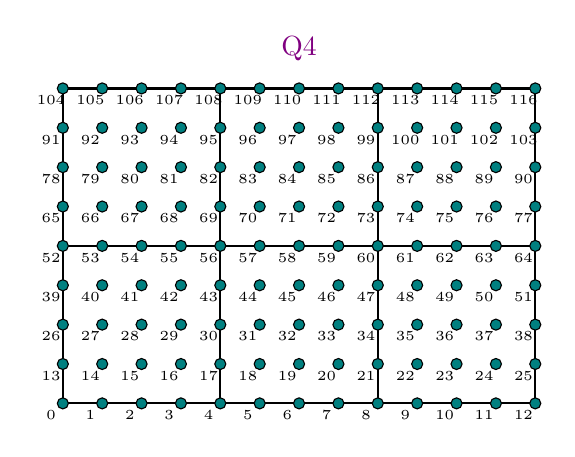
\begin{tikzpicture} 
\node[violet] at (3,4.5) {Q4}; 
\draw[thick] (0,0) -- (6,0) -- (6,4) -- (0,4) -- cycle; 
\draw[thick] (0,2) -- (6,2) ; 
\draw[thick] (2,0) -- (2,4) ; 
\draw[thick] (4,0) -- (4,4) ; 
\draw[black,fill=teal] ( 0.000000 , 0.000000)     circle (2pt); 
\node[] at ( -0.150000, -0.150000 ) {\tiny 0 }; 
\draw[black,fill=teal] ( 0.500000 , 0.000000)     circle (2pt); 
\node[] at ( 0.350000, -0.150000 ) {\tiny 1 }; 
\draw[black,fill=teal] ( 1.000000 , 0.000000)     circle (2pt); 
\node[] at ( 0.850000, -0.150000 ) {\tiny 2 }; 
\draw[black,fill=teal] ( 1.500000 , 0.000000)     circle (2pt); 
\node[] at ( 1.350000, -0.150000 ) {\tiny 3 }; 
\draw[black,fill=teal] ( 2.000000 , 0.000000)     circle (2pt); 
\node[] at ( 1.850000, -0.150000 ) {\tiny 4 }; 
\draw[black,fill=teal] ( 2.500000 , 0.000000)     circle (2pt); 
\node[] at ( 2.350000, -0.150000 ) {\tiny 5 }; 
\draw[black,fill=teal] ( 3.000000 , 0.000000)     circle (2pt); 
\node[] at ( 2.850000, -0.150000 ) {\tiny 6 }; 
\draw[black,fill=teal] ( 3.500000 , 0.000000)     circle (2pt); 
\node[] at ( 3.350000, -0.150000 ) {\tiny 7 }; 
\draw[black,fill=teal] ( 4.000000 , 0.000000)     circle (2pt); 
\node[] at ( 3.850000, -0.150000 ) {\tiny 8 }; 
\draw[black,fill=teal] ( 4.500000 , 0.000000)     circle (2pt); 
\node[] at ( 4.350000, -0.150000 ) {\tiny 9 }; 
\draw[black,fill=teal] ( 5.000000 , 0.000000)     circle (2pt); 
\node[] at ( 4.850000, -0.150000 ) {\tiny 10 }; 
\draw[black,fill=teal] ( 5.500000 , 0.000000)     circle (2pt); 
\node[] at ( 5.350000, -0.150000 ) {\tiny 11 }; 
\draw[black,fill=teal] ( 6.000000 , 0.000000)     circle (2pt); 
\node[] at ( 5.850000, -0.150000 ) {\tiny 12 }; 
\draw[black,fill=teal] ( 0.000000 , 0.500000)     circle (2pt); 
\node[] at ( -0.150000, 0.350000 ) {\tiny 13 }; 
\draw[black,fill=teal] ( 0.500000 , 0.500000)     circle (2pt); 
\node[] at ( 0.350000, 0.350000 ) {\tiny 14 }; 
\draw[black,fill=teal] ( 1.000000 , 0.500000)     circle (2pt); 
\node[] at ( 0.850000, 0.350000 ) {\tiny 15 }; 
\draw[black,fill=teal] ( 1.500000 , 0.500000)     circle (2pt); 
\node[] at ( 1.350000, 0.350000 ) {\tiny 16 }; 
\draw[black,fill=teal] ( 2.000000 , 0.500000)     circle (2pt); 
\node[] at ( 1.850000, 0.350000 ) {\tiny 17 }; 
\draw[black,fill=teal] ( 2.500000 , 0.500000)     circle (2pt); 
\node[] at ( 2.350000, 0.350000 ) {\tiny 18 }; 
\draw[black,fill=teal] ( 3.000000 , 0.500000)     circle (2pt); 
\node[] at ( 2.850000, 0.350000 ) {\tiny 19 }; 
\draw[black,fill=teal] ( 3.500000 , 0.500000)     circle (2pt); 
\node[] at ( 3.350000, 0.350000 ) {\tiny 20 }; 
\draw[black,fill=teal] ( 4.000000 , 0.500000)     circle (2pt); 
\node[] at ( 3.850000, 0.350000 ) {\tiny 21 }; 
\draw[black,fill=teal] ( 4.500000 , 0.500000)     circle (2pt); 
\node[] at ( 4.350000, 0.350000 ) {\tiny 22 }; 
\draw[black,fill=teal] ( 5.000000 , 0.500000)     circle (2pt); 
\node[] at ( 4.850000, 0.350000 ) {\tiny 23 }; 
\draw[black,fill=teal] ( 5.500000 , 0.500000)     circle (2pt); 
\node[] at ( 5.350000, 0.350000 ) {\tiny 24 }; 
\draw[black,fill=teal] ( 6.000000 , 0.500000)     circle (2pt); 
\node[] at ( 5.850000, 0.350000 ) {\tiny 25 }; 
\draw[black,fill=teal] ( 0.000000 , 1.000000)     circle (2pt); 
\node[] at ( -0.150000, 0.850000 ) {\tiny 26 }; 
\draw[black,fill=teal] ( 0.500000 , 1.000000)     circle (2pt); 
\node[] at ( 0.350000, 0.850000 ) {\tiny 27 }; 
\draw[black,fill=teal] ( 1.000000 , 1.000000)     circle (2pt); 
\node[] at ( 0.850000, 0.850000 ) {\tiny 28 }; 
\draw[black,fill=teal] ( 1.500000 , 1.000000)     circle (2pt); 
\node[] at ( 1.350000, 0.850000 ) {\tiny 29 }; 
\draw[black,fill=teal] ( 2.000000 , 1.000000)     circle (2pt); 
\node[] at ( 1.850000, 0.850000 ) {\tiny 30 }; 
\draw[black,fill=teal] ( 2.500000 , 1.000000)     circle (2pt); 
\node[] at ( 2.350000, 0.850000 ) {\tiny 31 }; 
\draw[black,fill=teal] ( 3.000000 , 1.000000)     circle (2pt); 
\node[] at ( 2.850000, 0.850000 ) {\tiny 32 }; 
\draw[black,fill=teal] ( 3.500000 , 1.000000)     circle (2pt); 
\node[] at ( 3.350000, 0.850000 ) {\tiny 33 }; 
\draw[black,fill=teal] ( 4.000000 , 1.000000)     circle (2pt); 
\node[] at ( 3.850000, 0.850000 ) {\tiny 34 }; 
\draw[black,fill=teal] ( 4.500000 , 1.000000)     circle (2pt); 
\node[] at ( 4.350000, 0.850000 ) {\tiny 35 }; 
\draw[black,fill=teal] ( 5.000000 , 1.000000)     circle (2pt); 
\node[] at ( 4.850000, 0.850000 ) {\tiny 36 }; 
\draw[black,fill=teal] ( 5.500000 , 1.000000)     circle (2pt); 
\node[] at ( 5.350000, 0.850000 ) {\tiny 37 }; 
\draw[black,fill=teal] ( 6.000000 , 1.000000)     circle (2pt); 
\node[] at ( 5.850000, 0.850000 ) {\tiny 38 }; 
\draw[black,fill=teal] ( 0.000000 , 1.500000)     circle (2pt); 
\node[] at ( -0.150000, 1.350000 ) {\tiny 39 }; 
\draw[black,fill=teal] ( 0.500000 , 1.500000)     circle (2pt); 
\node[] at ( 0.350000, 1.350000 ) {\tiny 40 }; 
\draw[black,fill=teal] ( 1.000000 , 1.500000)     circle (2pt); 
\node[] at ( 0.850000, 1.350000 ) {\tiny 41 }; 
\draw[black,fill=teal] ( 1.500000 , 1.500000)     circle (2pt); 
\node[] at ( 1.350000, 1.350000 ) {\tiny 42 }; 
\draw[black,fill=teal] ( 2.000000 , 1.500000)     circle (2pt); 
\node[] at ( 1.850000, 1.350000 ) {\tiny 43 }; 
\draw[black,fill=teal] ( 2.500000 , 1.500000)     circle (2pt); 
\node[] at ( 2.350000, 1.350000 ) {\tiny 44 }; 
\draw[black,fill=teal] ( 3.000000 , 1.500000)     circle (2pt); 
\node[] at ( 2.850000, 1.350000 ) {\tiny 45 }; 
\draw[black,fill=teal] ( 3.500000 , 1.500000)     circle (2pt); 
\node[] at ( 3.350000, 1.350000 ) {\tiny 46 }; 
\draw[black,fill=teal] ( 4.000000 , 1.500000)     circle (2pt); 
\node[] at ( 3.850000, 1.350000 ) {\tiny 47 }; 
\draw[black,fill=teal] ( 4.500000 , 1.500000)     circle (2pt); 
\node[] at ( 4.350000, 1.350000 ) {\tiny 48 }; 
\draw[black,fill=teal] ( 5.000000 , 1.500000)     circle (2pt); 
\node[] at ( 4.850000, 1.350000 ) {\tiny 49 }; 
\draw[black,fill=teal] ( 5.500000 , 1.500000)     circle (2pt); 
\node[] at ( 5.350000, 1.350000 ) {\tiny 50 }; 
\draw[black,fill=teal] ( 6.000000 , 1.500000)     circle (2pt); 
\node[] at ( 5.850000, 1.350000 ) {\tiny 51 }; 
\draw[black,fill=teal] ( 0.000000 , 2.000000)     circle (2pt); 
\node[] at ( -0.150000, 1.850000 ) {\tiny 52 }; 
\draw[black,fill=teal] ( 0.500000 , 2.000000)     circle (2pt); 
\node[] at ( 0.350000, 1.850000 ) {\tiny 53 }; 
\draw[black,fill=teal] ( 1.000000 , 2.000000)     circle (2pt); 
\node[] at ( 0.850000, 1.850000 ) {\tiny 54 }; 
\draw[black,fill=teal] ( 1.500000 , 2.000000)     circle (2pt); 
\node[] at ( 1.350000, 1.850000 ) {\tiny 55 }; 
\draw[black,fill=teal] ( 2.000000 , 2.000000)     circle (2pt); 
\node[] at ( 1.850000, 1.850000 ) {\tiny 56 }; 
\draw[black,fill=teal] ( 2.500000 , 2.000000)     circle (2pt); 
\node[] at ( 2.350000, 1.850000 ) {\tiny 57 }; 
\draw[black,fill=teal] ( 3.000000 , 2.000000)     circle (2pt); 
\node[] at ( 2.850000, 1.850000 ) {\tiny 58 }; 
\draw[black,fill=teal] ( 3.500000 , 2.000000)     circle (2pt); 
\node[] at ( 3.350000, 1.850000 ) {\tiny 59 }; 
\draw[black,fill=teal] ( 4.000000 , 2.000000)     circle (2pt); 
\node[] at ( 3.850000, 1.850000 ) {\tiny 60 }; 
\draw[black,fill=teal] ( 4.500000 , 2.000000)     circle (2pt); 
\node[] at ( 4.350000, 1.850000 ) {\tiny 61 }; 
\draw[black,fill=teal] ( 5.000000 , 2.000000)     circle (2pt); 
\node[] at ( 4.850000, 1.850000 ) {\tiny 62 }; 
\draw[black,fill=teal] ( 5.500000 , 2.000000)     circle (2pt); 
\node[] at ( 5.350000, 1.850000 ) {\tiny 63 }; 
\draw[black,fill=teal] ( 6.000000 , 2.000000)     circle (2pt); 
\node[] at ( 5.850000, 1.850000 ) {\tiny 64 }; 
\draw[black,fill=teal] ( 0.000000 , 2.500000)     circle (2pt); 
\node[] at ( -0.150000, 2.350000 ) {\tiny 65 }; 
\draw[black,fill=teal] ( 0.500000 , 2.500000)     circle (2pt); 
\node[] at ( 0.350000, 2.350000 ) {\tiny 66 }; 
\draw[black,fill=teal] ( 1.000000 , 2.500000)     circle (2pt); 
\node[] at ( 0.850000, 2.350000 ) {\tiny 67 }; 
\draw[black,fill=teal] ( 1.500000 , 2.500000)     circle (2pt); 
\node[] at ( 1.350000, 2.350000 ) {\tiny 68 }; 
\draw[black,fill=teal] ( 2.000000 , 2.500000)     circle (2pt); 
\node[] at ( 1.850000, 2.350000 ) {\tiny 69 }; 
\draw[black,fill=teal] ( 2.500000 , 2.500000)     circle (2pt); 
\node[] at ( 2.350000, 2.350000 ) {\tiny 70 }; 
\draw[black,fill=teal] ( 3.000000 , 2.500000)     circle (2pt); 
\node[] at ( 2.850000, 2.350000 ) {\tiny 71 }; 
\draw[black,fill=teal] ( 3.500000 , 2.500000)     circle (2pt); 
\node[] at ( 3.350000, 2.350000 ) {\tiny 72 }; 
\draw[black,fill=teal] ( 4.000000 , 2.500000)     circle (2pt); 
\node[] at ( 3.850000, 2.350000 ) {\tiny 73 }; 
\draw[black,fill=teal] ( 4.500000 , 2.500000)     circle (2pt); 
\node[] at ( 4.350000, 2.350000 ) {\tiny 74 }; 
\draw[black,fill=teal] ( 5.000000 , 2.500000)     circle (2pt); 
\node[] at ( 4.850000, 2.350000 ) {\tiny 75 }; 
\draw[black,fill=teal] ( 5.500000 , 2.500000)     circle (2pt); 
\node[] at ( 5.350000, 2.350000 ) {\tiny 76 }; 
\draw[black,fill=teal] ( 6.000000 , 2.500000)     circle (2pt); 
\node[] at ( 5.850000, 2.350000 ) {\tiny 77 }; 
\draw[black,fill=teal] ( 0.000000 , 3.000000)     circle (2pt); 
\node[] at ( -0.150000, 2.850000 ) {\tiny 78 }; 
\draw[black,fill=teal] ( 0.500000 , 3.000000)     circle (2pt); 
\node[] at ( 0.350000, 2.850000 ) {\tiny 79 }; 
\draw[black,fill=teal] ( 1.000000 , 3.000000)     circle (2pt); 
\node[] at ( 0.850000, 2.850000 ) {\tiny 80 }; 
\draw[black,fill=teal] ( 1.500000 , 3.000000)     circle (2pt); 
\node[] at ( 1.350000, 2.850000 ) {\tiny 81 }; 
\draw[black,fill=teal] ( 2.000000 , 3.000000)     circle (2pt); 
\node[] at ( 1.850000, 2.850000 ) {\tiny 82 }; 
\draw[black,fill=teal] ( 2.500000 , 3.000000)     circle (2pt); 
\node[] at ( 2.350000, 2.850000 ) {\tiny 83 }; 
\draw[black,fill=teal] ( 3.000000 , 3.000000)     circle (2pt); 
\node[] at ( 2.850000, 2.850000 ) {\tiny 84 }; 
\draw[black,fill=teal] ( 3.500000 , 3.000000)     circle (2pt); 
\node[] at ( 3.350000, 2.850000 ) {\tiny 85 }; 
\draw[black,fill=teal] ( 4.000000 , 3.000000)     circle (2pt); 
\node[] at ( 3.850000, 2.850000 ) {\tiny 86 }; 
\draw[black,fill=teal] ( 4.500000 , 3.000000)     circle (2pt); 
\node[] at ( 4.350000, 2.850000 ) {\tiny 87 }; 
\draw[black,fill=teal] ( 5.000000 , 3.000000)     circle (2pt); 
\node[] at ( 4.850000, 2.850000 ) {\tiny 88 }; 
\draw[black,fill=teal] ( 5.500000 , 3.000000)     circle (2pt); 
\node[] at ( 5.350000, 2.850000 ) {\tiny 89 }; 
\draw[black,fill=teal] ( 6.000000 , 3.000000)     circle (2pt); 
\node[] at ( 5.850000, 2.850000 ) {\tiny 90 }; 
\draw[black,fill=teal] ( 0.000000 , 3.500000)     circle (2pt); 
\node[] at ( -0.150000, 3.350000 ) {\tiny 91 }; 
\draw[black,fill=teal] ( 0.500000 , 3.500000)     circle (2pt); 
\node[] at ( 0.350000, 3.350000 ) {\tiny 92 }; 
\draw[black,fill=teal] ( 1.000000 , 3.500000)     circle (2pt); 
\node[] at ( 0.850000, 3.350000 ) {\tiny 93 }; 
\draw[black,fill=teal] ( 1.500000 , 3.500000)     circle (2pt); 
\node[] at ( 1.350000, 3.350000 ) {\tiny 94 }; 
\draw[black,fill=teal] ( 2.000000 , 3.500000)     circle (2pt); 
\node[] at ( 1.850000, 3.350000 ) {\tiny 95 }; 
\draw[black,fill=teal] ( 2.500000 , 3.500000)     circle (2pt); 
\node[] at ( 2.350000, 3.350000 ) {\tiny 96 }; 
\draw[black,fill=teal] ( 3.000000 , 3.500000)     circle (2pt); 
\node[] at ( 2.850000, 3.350000 ) {\tiny 97 }; 
\draw[black,fill=teal] ( 3.500000 , 3.500000)     circle (2pt); 
\node[] at ( 3.350000, 3.350000 ) {\tiny 98 }; 
\draw[black,fill=teal] ( 4.000000 , 3.500000)     circle (2pt); 
\node[] at ( 3.850000, 3.350000 ) {\tiny 99 }; 
\draw[black,fill=teal] ( 4.500000 , 3.500000)     circle (2pt); 
\node[] at ( 4.350000, 3.350000 ) {\tiny 100 }; 
\draw[black,fill=teal] ( 5.000000 , 3.500000)     circle (2pt); 
\node[] at ( 4.850000, 3.350000 ) {\tiny 101 }; 
\draw[black,fill=teal] ( 5.500000 , 3.500000)     circle (2pt); 
\node[] at ( 5.350000, 3.350000 ) {\tiny 102 }; 
\draw[black,fill=teal] ( 6.000000 , 3.500000)     circle (2pt); 
\node[] at ( 5.850000, 3.350000 ) {\tiny 103 }; 
\draw[black,fill=teal] ( 0.000000 , 4.000000)     circle (2pt); 
\node[] at ( -0.150000, 3.850000 ) {\tiny 104 }; 
\draw[black,fill=teal] ( 0.500000 , 4.000000)     circle (2pt); 
\node[] at ( 0.350000, 3.850000 ) {\tiny 105 }; 
\draw[black,fill=teal] ( 1.000000 , 4.000000)     circle (2pt); 
\node[] at ( 0.850000, 3.850000 ) {\tiny 106 }; 
\draw[black,fill=teal] ( 1.500000 , 4.000000)     circle (2pt); 
\node[] at ( 1.350000, 3.850000 ) {\tiny 107 }; 
\draw[black,fill=teal] ( 2.000000 , 4.000000)     circle (2pt); 
\node[] at ( 1.850000, 3.850000 ) {\tiny 108 }; 
\draw[black,fill=teal] ( 2.500000 , 4.000000)     circle (2pt); 
\node[] at ( 2.350000, 3.850000 ) {\tiny 109 }; 
\draw[black,fill=teal] ( 3.000000 , 4.000000)     circle (2pt); 
\node[] at ( 2.850000, 3.850000 ) {\tiny 110 }; 
\draw[black,fill=teal] ( 3.500000 , 4.000000)     circle (2pt); 
\node[] at ( 3.350000, 3.850000 ) {\tiny 111 }; 
\draw[black,fill=teal] ( 4.000000 , 4.000000)     circle (2pt); 
\node[] at ( 3.850000, 3.850000 ) {\tiny 112 }; 
\draw[black,fill=teal] ( 4.500000 , 4.000000)     circle (2pt); 
\node[] at ( 4.350000, 3.850000 ) {\tiny 113 }; 
\draw[black,fill=teal] ( 5.000000 , 4.000000)     circle (2pt); 
\node[] at ( 4.850000, 3.850000 ) {\tiny 114 }; 
\draw[black,fill=teal] ( 5.500000 , 4.000000)     circle (2pt); 
\node[] at ( 5.350000, 3.850000 ) {\tiny 115 }; 
\draw[black,fill=teal] ( 6.000000 , 4.000000)     circle (2pt); 
\node[] at ( 5.850000, 3.850000 ) {\tiny 116 }; 
\end{tikzpicture} 
\end{center} 


\begin{tiny}
\verbatiminput{python_codes/fieldstone_120/spaces/iconV_elt1_Q4.ascii}
\end{tiny}
\end{multicols}

\newpage
%------------------
\begin{multicols}{2}
\begin{center} 
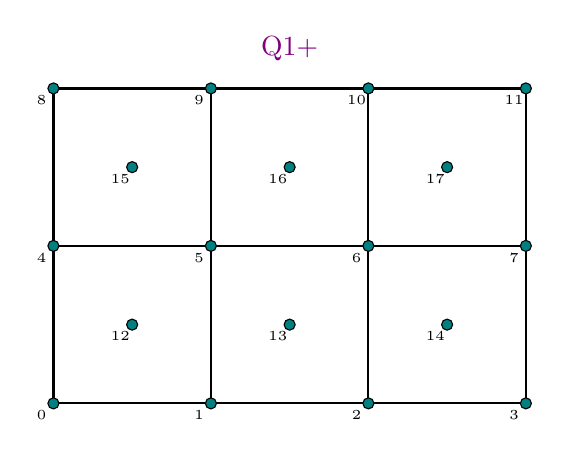
\begin{tikzpicture} 
\node[violet] at (3,4.5) {Q1+}; 
\draw[thick] (0,0) -- (6,0) -- (6,4) -- (0,4) -- cycle; 
\draw[thick] (0,2) -- (6,2) ; 
\draw[thick] (2,0) -- (2,4) ; 
\draw[thick] (4,0) -- (4,4) ; 
\draw[black,fill=teal] ( 0.000000 , 0.000000)     circle (2pt); 
\node[] at ( -0.150000, -0.150000 ) {\tiny 0 }; 
\draw[black,fill=teal] ( 2.000000 , 0.000000)     circle (2pt); 
\node[] at ( 1.850000, -0.150000 ) {\tiny 1 }; 
\draw[black,fill=teal] ( 4.000000 , 0.000000)     circle (2pt); 
\node[] at ( 3.850000, -0.150000 ) {\tiny 2 }; 
\draw[black,fill=teal] ( 6.000000 , 0.000000)     circle (2pt); 
\node[] at ( 5.850000, -0.150000 ) {\tiny 3 }; 
\draw[black,fill=teal] ( 0.000000 , 2.000000)     circle (2pt); 
\node[] at ( -0.150000, 1.850000 ) {\tiny 4 }; 
\draw[black,fill=teal] ( 2.000000 , 2.000000)     circle (2pt); 
\node[] at ( 1.850000, 1.850000 ) {\tiny 5 }; 
\draw[black,fill=teal] ( 4.000000 , 2.000000)     circle (2pt); 
\node[] at ( 3.850000, 1.850000 ) {\tiny 6 }; 
\draw[black,fill=teal] ( 6.000000 , 2.000000)     circle (2pt); 
\node[] at ( 5.850000, 1.850000 ) {\tiny 7 }; 
\draw[black,fill=teal] ( 0.000000 , 4.000000)     circle (2pt); 
\node[] at ( -0.150000, 3.850000 ) {\tiny 8 }; 
\draw[black,fill=teal] ( 2.000000 , 4.000000)     circle (2pt); 
\node[] at ( 1.850000, 3.850000 ) {\tiny 9 }; 
\draw[black,fill=teal] ( 4.000000 , 4.000000)     circle (2pt); 
\node[] at ( 3.850000, 3.850000 ) {\tiny 10 }; 
\draw[black,fill=teal] ( 6.000000 , 4.000000)     circle (2pt); 
\node[] at ( 5.850000, 3.850000 ) {\tiny 11 }; 
\draw[black,fill=teal] ( 1.000000 , 1.000000)     circle (2pt); 
\node[] at ( 0.850000, 0.850000 ) {\tiny 12 }; 
\draw[black,fill=teal] ( 3.000000 , 1.000000)     circle (2pt); 
\node[] at ( 2.850000, 0.850000 ) {\tiny 13 }; 
\draw[black,fill=teal] ( 5.000000 , 1.000000)     circle (2pt); 
\node[] at ( 4.850000, 0.850000 ) {\tiny 14 }; 
\draw[black,fill=teal] ( 1.000000 , 3.000000)     circle (2pt); 
\node[] at ( 0.850000, 2.850000 ) {\tiny 15 }; 
\draw[black,fill=teal] ( 3.000000 , 3.000000)     circle (2pt); 
\node[] at ( 2.850000, 2.850000 ) {\tiny 16 }; 
\draw[black,fill=teal] ( 5.000000 , 3.000000)     circle (2pt); 
\node[] at ( 4.850000, 2.850000 ) {\tiny 17 }; 
\end{tikzpicture} 
\end{center} 


\begin{tiny}
\verbatiminput{python_codes/fieldstone_120/spaces/iconV_elt1_Q1+.ascii}
\end{tiny}
\end{multicols}

%------------------
\begin{multicols}{2}
\begin{center} 
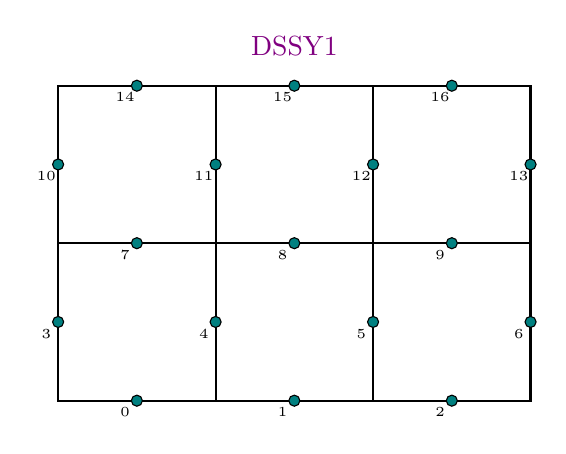
\begin{tikzpicture} 
\node[violet] at (3,4.5) {DSSY1}; 
\draw[thick] (0,0) -- (6,0) -- (6,4) -- (0,4) -- cycle; 
\draw[thick] (0,2) -- (6,2) ; 
\draw[thick] (2,0) -- (2,4) ; 
\draw[thick] (4,0) -- (4,4) ; 
\draw[black,fill=teal] ( 1.000000 , 0.000000)     circle (2pt); 
\node[] at ( 0.850000, -0.150000 ) {\tiny 0 }; 
\draw[black,fill=teal] ( 3.000000 , 0.000000)     circle (2pt); 
\node[] at ( 2.850000, -0.150000 ) {\tiny 1 }; 
\draw[black,fill=teal] ( 5.000000 , 0.000000)     circle (2pt); 
\node[] at ( 4.850000, -0.150000 ) {\tiny 2 }; 
\draw[black,fill=teal] ( 0.000000 , 1.000000)     circle (2pt); 
\node[] at ( -0.150000, 0.850000 ) {\tiny 3 }; 
\draw[black,fill=teal] ( 2.000000 , 1.000000)     circle (2pt); 
\node[] at ( 1.850000, 0.850000 ) {\tiny 4 }; 
\draw[black,fill=teal] ( 4.000000 , 1.000000)     circle (2pt); 
\node[] at ( 3.850000, 0.850000 ) {\tiny 5 }; 
\draw[black,fill=teal] ( 6.000000 , 1.000000)     circle (2pt); 
\node[] at ( 5.850000, 0.850000 ) {\tiny 6 }; 
\draw[black,fill=teal] ( 1.000000 , 2.000000)     circle (2pt); 
\node[] at ( 0.850000, 1.850000 ) {\tiny 7 }; 
\draw[black,fill=teal] ( 3.000000 , 2.000000)     circle (2pt); 
\node[] at ( 2.850000, 1.850000 ) {\tiny 8 }; 
\draw[black,fill=teal] ( 5.000000 , 2.000000)     circle (2pt); 
\node[] at ( 4.850000, 1.850000 ) {\tiny 9 }; 
\draw[black,fill=teal] ( 0.000000 , 3.000000)     circle (2pt); 
\node[] at ( -0.150000, 2.850000 ) {\tiny 10 }; 
\draw[black,fill=teal] ( 2.000000 , 3.000000)     circle (2pt); 
\node[] at ( 1.850000, 2.850000 ) {\tiny 11 }; 
\draw[black,fill=teal] ( 4.000000 , 3.000000)     circle (2pt); 
\node[] at ( 3.850000, 2.850000 ) {\tiny 12 }; 
\draw[black,fill=teal] ( 6.000000 , 3.000000)     circle (2pt); 
\node[] at ( 5.850000, 2.850000 ) {\tiny 13 }; 
\draw[black,fill=teal] ( 1.000000 , 4.000000)     circle (2pt); 
\node[] at ( 0.850000, 3.850000 ) {\tiny 14 }; 
\draw[black,fill=teal] ( 3.000000 , 4.000000)     circle (2pt); 
\node[] at ( 2.850000, 3.850000 ) {\tiny 15 }; 
\draw[black,fill=teal] ( 5.000000 , 4.000000)     circle (2pt); 
\node[] at ( 4.850000, 3.850000 ) {\tiny 16 }; 
\end{tikzpicture} 
\end{center} 


\begin{tiny}
\verbatiminput{python_codes/fieldstone_120/spaces/iconV_elt1_DSSY1.ascii}
\end{tiny}
\end{multicols}

%------------------
%\begin{multicols}{2}
%\begin{center} 
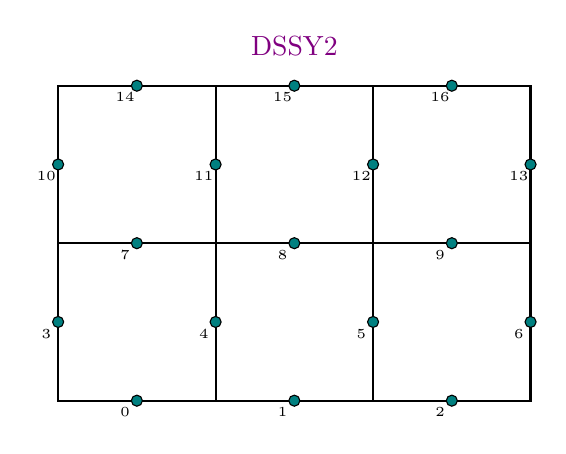
\begin{tikzpicture} 
\node[violet] at (3,4.5) {DSSY2}; 
\draw[thick] (0,0) -- (6,0) -- (6,4) -- (0,4) -- cycle; 
\draw[thick] (0,2) -- (6,2) ; 
\draw[thick] (2,0) -- (2,4) ; 
\draw[thick] (4,0) -- (4,4) ; 
\draw[black,fill=teal] ( 1.000000 , 0.000000)     circle (2pt); 
\node[] at ( 0.850000, -0.150000 ) {\tiny 0 }; 
\draw[black,fill=teal] ( 3.000000 , 0.000000)     circle (2pt); 
\node[] at ( 2.850000, -0.150000 ) {\tiny 1 }; 
\draw[black,fill=teal] ( 5.000000 , 0.000000)     circle (2pt); 
\node[] at ( 4.850000, -0.150000 ) {\tiny 2 }; 
\draw[black,fill=teal] ( 0.000000 , 1.000000)     circle (2pt); 
\node[] at ( -0.150000, 0.850000 ) {\tiny 3 }; 
\draw[black,fill=teal] ( 2.000000 , 1.000000)     circle (2pt); 
\node[] at ( 1.850000, 0.850000 ) {\tiny 4 }; 
\draw[black,fill=teal] ( 4.000000 , 1.000000)     circle (2pt); 
\node[] at ( 3.850000, 0.850000 ) {\tiny 5 }; 
\draw[black,fill=teal] ( 6.000000 , 1.000000)     circle (2pt); 
\node[] at ( 5.850000, 0.850000 ) {\tiny 6 }; 
\draw[black,fill=teal] ( 1.000000 , 2.000000)     circle (2pt); 
\node[] at ( 0.850000, 1.850000 ) {\tiny 7 }; 
\draw[black,fill=teal] ( 3.000000 , 2.000000)     circle (2pt); 
\node[] at ( 2.850000, 1.850000 ) {\tiny 8 }; 
\draw[black,fill=teal] ( 5.000000 , 2.000000)     circle (2pt); 
\node[] at ( 4.850000, 1.850000 ) {\tiny 9 }; 
\draw[black,fill=teal] ( 0.000000 , 3.000000)     circle (2pt); 
\node[] at ( -0.150000, 2.850000 ) {\tiny 10 }; 
\draw[black,fill=teal] ( 2.000000 , 3.000000)     circle (2pt); 
\node[] at ( 1.850000, 2.850000 ) {\tiny 11 }; 
\draw[black,fill=teal] ( 4.000000 , 3.000000)     circle (2pt); 
\node[] at ( 3.850000, 2.850000 ) {\tiny 12 }; 
\draw[black,fill=teal] ( 6.000000 , 3.000000)     circle (2pt); 
\node[] at ( 5.850000, 2.850000 ) {\tiny 13 }; 
\draw[black,fill=teal] ( 1.000000 , 4.000000)     circle (2pt); 
\node[] at ( 0.850000, 3.850000 ) {\tiny 14 }; 
\draw[black,fill=teal] ( 3.000000 , 4.000000)     circle (2pt); 
\node[] at ( 2.850000, 3.850000 ) {\tiny 15 }; 
\draw[black,fill=teal] ( 5.000000 , 4.000000)     circle (2pt); 
\node[] at ( 4.850000, 3.850000 ) {\tiny 16 }; 
\end{tikzpicture} 
\end{center} 


%\begin{tiny}
%\verbatiminput{python_codes/fieldstone_120/spaces/iconV_elt1_DSSY2.ascii}
%\end{tiny}
%\end{multicols}

%------------------
\begin{multicols}{2}
\begin{center} 
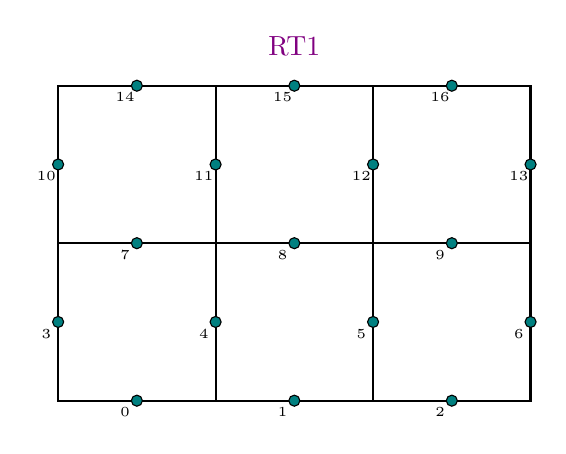
\begin{tikzpicture} 
\node[violet] at (3,4.5) {RT1}; 
\draw[thick] (0,0) -- (6,0) -- (6,4) -- (0,4) -- cycle; 
\draw[thick] (0,2) -- (6,2) ; 
\draw[thick] (2,0) -- (2,4) ; 
\draw[thick] (4,0) -- (4,4) ; 
\draw[black,fill=teal] ( 1.000000 , 0.000000)     circle (2pt); 
\node[] at ( 0.850000, -0.150000 ) {\tiny 0 }; 
\draw[black,fill=teal] ( 3.000000 , 0.000000)     circle (2pt); 
\node[] at ( 2.850000, -0.150000 ) {\tiny 1 }; 
\draw[black,fill=teal] ( 5.000000 , 0.000000)     circle (2pt); 
\node[] at ( 4.850000, -0.150000 ) {\tiny 2 }; 
\draw[black,fill=teal] ( 0.000000 , 1.000000)     circle (2pt); 
\node[] at ( -0.150000, 0.850000 ) {\tiny 3 }; 
\draw[black,fill=teal] ( 2.000000 , 1.000000)     circle (2pt); 
\node[] at ( 1.850000, 0.850000 ) {\tiny 4 }; 
\draw[black,fill=teal] ( 4.000000 , 1.000000)     circle (2pt); 
\node[] at ( 3.850000, 0.850000 ) {\tiny 5 }; 
\draw[black,fill=teal] ( 6.000000 , 1.000000)     circle (2pt); 
\node[] at ( 5.850000, 0.850000 ) {\tiny 6 }; 
\draw[black,fill=teal] ( 1.000000 , 2.000000)     circle (2pt); 
\node[] at ( 0.850000, 1.850000 ) {\tiny 7 }; 
\draw[black,fill=teal] ( 3.000000 , 2.000000)     circle (2pt); 
\node[] at ( 2.850000, 1.850000 ) {\tiny 8 }; 
\draw[black,fill=teal] ( 5.000000 , 2.000000)     circle (2pt); 
\node[] at ( 4.850000, 1.850000 ) {\tiny 9 }; 
\draw[black,fill=teal] ( 0.000000 , 3.000000)     circle (2pt); 
\node[] at ( -0.150000, 2.850000 ) {\tiny 10 }; 
\draw[black,fill=teal] ( 2.000000 , 3.000000)     circle (2pt); 
\node[] at ( 1.850000, 2.850000 ) {\tiny 11 }; 
\draw[black,fill=teal] ( 4.000000 , 3.000000)     circle (2pt); 
\node[] at ( 3.850000, 2.850000 ) {\tiny 12 }; 
\draw[black,fill=teal] ( 6.000000 , 3.000000)     circle (2pt); 
\node[] at ( 5.850000, 2.850000 ) {\tiny 13 }; 
\draw[black,fill=teal] ( 1.000000 , 4.000000)     circle (2pt); 
\node[] at ( 0.850000, 3.850000 ) {\tiny 14 }; 
\draw[black,fill=teal] ( 3.000000 , 4.000000)     circle (2pt); 
\node[] at ( 2.850000, 3.850000 ) {\tiny 15 }; 
\draw[black,fill=teal] ( 5.000000 , 4.000000)     circle (2pt); 
\node[] at ( 4.850000, 3.850000 ) {\tiny 16 }; 
\end{tikzpicture} 
\end{center} 


\begin{tiny}
\verbatiminput{python_codes/fieldstone_120/spaces/iconV_elt1_RT1.ascii}
\end{tiny}
\end{multicols}

%------------------
%\begin{multicols}{2}
%\begin{center} 
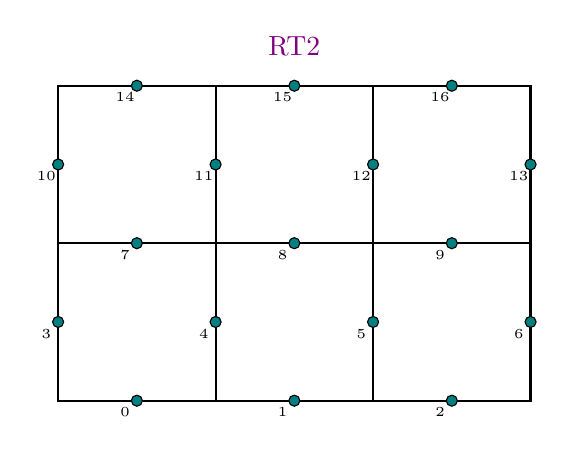
\begin{tikzpicture} 
\node[violet] at (3,4.5) {RT2}; 
\draw[thick] (0,0) -- (6,0) -- (6,4) -- (0,4) -- cycle; 
\draw[thick] (0,2) -- (6,2) ; 
\draw[thick] (2,0) -- (2,4) ; 
\draw[thick] (4,0) -- (4,4) ; 
\draw[black,fill=teal] ( 1.000000 , 0.000000)     circle (2pt); 
\node[] at ( 0.850000, -0.150000 ) {\tiny 0 }; 
\draw[black,fill=teal] ( 3.000000 , 0.000000)     circle (2pt); 
\node[] at ( 2.850000, -0.150000 ) {\tiny 1 }; 
\draw[black,fill=teal] ( 5.000000 , 0.000000)     circle (2pt); 
\node[] at ( 4.850000, -0.150000 ) {\tiny 2 }; 
\draw[black,fill=teal] ( 0.000000 , 1.000000)     circle (2pt); 
\node[] at ( -0.150000, 0.850000 ) {\tiny 3 }; 
\draw[black,fill=teal] ( 2.000000 , 1.000000)     circle (2pt); 
\node[] at ( 1.850000, 0.850000 ) {\tiny 4 }; 
\draw[black,fill=teal] ( 4.000000 , 1.000000)     circle (2pt); 
\node[] at ( 3.850000, 0.850000 ) {\tiny 5 }; 
\draw[black,fill=teal] ( 6.000000 , 1.000000)     circle (2pt); 
\node[] at ( 5.850000, 0.850000 ) {\tiny 6 }; 
\draw[black,fill=teal] ( 1.000000 , 2.000000)     circle (2pt); 
\node[] at ( 0.850000, 1.850000 ) {\tiny 7 }; 
\draw[black,fill=teal] ( 3.000000 , 2.000000)     circle (2pt); 
\node[] at ( 2.850000, 1.850000 ) {\tiny 8 }; 
\draw[black,fill=teal] ( 5.000000 , 2.000000)     circle (2pt); 
\node[] at ( 4.850000, 1.850000 ) {\tiny 9 }; 
\draw[black,fill=teal] ( 0.000000 , 3.000000)     circle (2pt); 
\node[] at ( -0.150000, 2.850000 ) {\tiny 10 }; 
\draw[black,fill=teal] ( 2.000000 , 3.000000)     circle (2pt); 
\node[] at ( 1.850000, 2.850000 ) {\tiny 11 }; 
\draw[black,fill=teal] ( 4.000000 , 3.000000)     circle (2pt); 
\node[] at ( 3.850000, 2.850000 ) {\tiny 12 }; 
\draw[black,fill=teal] ( 6.000000 , 3.000000)     circle (2pt); 
\node[] at ( 5.850000, 2.850000 ) {\tiny 13 }; 
\draw[black,fill=teal] ( 1.000000 , 4.000000)     circle (2pt); 
\node[] at ( 0.850000, 3.850000 ) {\tiny 14 }; 
\draw[black,fill=teal] ( 3.000000 , 4.000000)     circle (2pt); 
\node[] at ( 2.850000, 3.850000 ) {\tiny 15 }; 
\draw[black,fill=teal] ( 5.000000 , 4.000000)     circle (2pt); 
\node[] at ( 4.850000, 3.850000 ) {\tiny 16 }; 
\end{tikzpicture} 
\end{center} 


%\begin{tiny}
%\verbatiminput{python_codes/fieldstone_120/spaces/iconV_elt1_RT2.ascii}
%\end{tiny}
%\end{multicols}

%------------------
\begin{multicols}{2}
\begin{center} 
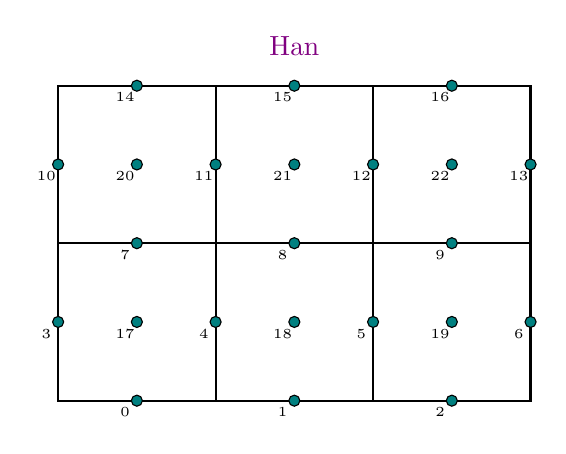
\begin{tikzpicture} 
\node[violet] at (3,4.5) {Han}; 
\draw[thick] (0,0) -- (6,0) -- (6,4) -- (0,4) -- cycle; 
\draw[thick] (0,2) -- (6,2) ; 
\draw[thick] (2,0) -- (2,4) ; 
\draw[thick] (4,0) -- (4,4) ; 
\draw[black,fill=teal] ( 1.000000 , 0.000000)     circle (2pt); 
\node[] at ( 0.850000, -0.150000 ) {\tiny 0 }; 
\draw[black,fill=teal] ( 3.000000 , 0.000000)     circle (2pt); 
\node[] at ( 2.850000, -0.150000 ) {\tiny 1 }; 
\draw[black,fill=teal] ( 5.000000 , 0.000000)     circle (2pt); 
\node[] at ( 4.850000, -0.150000 ) {\tiny 2 }; 
\draw[black,fill=teal] ( 0.000000 , 1.000000)     circle (2pt); 
\node[] at ( -0.150000, 0.850000 ) {\tiny 3 }; 
\draw[black,fill=teal] ( 2.000000 , 1.000000)     circle (2pt); 
\node[] at ( 1.850000, 0.850000 ) {\tiny 4 }; 
\draw[black,fill=teal] ( 4.000000 , 1.000000)     circle (2pt); 
\node[] at ( 3.850000, 0.850000 ) {\tiny 5 }; 
\draw[black,fill=teal] ( 6.000000 , 1.000000)     circle (2pt); 
\node[] at ( 5.850000, 0.850000 ) {\tiny 6 }; 
\draw[black,fill=teal] ( 1.000000 , 2.000000)     circle (2pt); 
\node[] at ( 0.850000, 1.850000 ) {\tiny 7 }; 
\draw[black,fill=teal] ( 3.000000 , 2.000000)     circle (2pt); 
\node[] at ( 2.850000, 1.850000 ) {\tiny 8 }; 
\draw[black,fill=teal] ( 5.000000 , 2.000000)     circle (2pt); 
\node[] at ( 4.850000, 1.850000 ) {\tiny 9 }; 
\draw[black,fill=teal] ( 0.000000 , 3.000000)     circle (2pt); 
\node[] at ( -0.150000, 2.850000 ) {\tiny 10 }; 
\draw[black,fill=teal] ( 2.000000 , 3.000000)     circle (2pt); 
\node[] at ( 1.850000, 2.850000 ) {\tiny 11 }; 
\draw[black,fill=teal] ( 4.000000 , 3.000000)     circle (2pt); 
\node[] at ( 3.850000, 2.850000 ) {\tiny 12 }; 
\draw[black,fill=teal] ( 6.000000 , 3.000000)     circle (2pt); 
\node[] at ( 5.850000, 2.850000 ) {\tiny 13 }; 
\draw[black,fill=teal] ( 1.000000 , 4.000000)     circle (2pt); 
\node[] at ( 0.850000, 3.850000 ) {\tiny 14 }; 
\draw[black,fill=teal] ( 3.000000 , 4.000000)     circle (2pt); 
\node[] at ( 2.850000, 3.850000 ) {\tiny 15 }; 
\draw[black,fill=teal] ( 5.000000 , 4.000000)     circle (2pt); 
\node[] at ( 4.850000, 3.850000 ) {\tiny 16 }; 
\draw[black,fill=teal] ( 1.000000 , 1.000000)     circle (2pt); 
\node[] at ( 0.850000, 0.850000 ) {\tiny 17 }; 
\draw[black,fill=teal] ( 3.000000 , 1.000000)     circle (2pt); 
\node[] at ( 2.850000, 0.850000 ) {\tiny 18 }; 
\draw[black,fill=teal] ( 5.000000 , 1.000000)     circle (2pt); 
\node[] at ( 4.850000, 0.850000 ) {\tiny 19 }; 
\draw[black,fill=teal] ( 1.000000 , 3.000000)     circle (2pt); 
\node[] at ( 0.850000, 2.850000 ) {\tiny 20 }; 
\draw[black,fill=teal] ( 3.000000 , 3.000000)     circle (2pt); 
\node[] at ( 2.850000, 2.850000 ) {\tiny 21 }; 
\draw[black,fill=teal] ( 5.000000 , 3.000000)     circle (2pt); 
\node[] at ( 4.850000, 2.850000 ) {\tiny 22 }; 
\end{tikzpicture} 
\end{center} 


\begin{tiny}
\verbatiminput{python_codes/fieldstone_120/spaces/iconV_elt1_Han.ascii}
\end{tiny}
\end{multicols}




\newpage
%-----------------------------------------------------------------------------
\subsection*{Python testers}

\begin{itemize}
\item \lstinline{tester1.py}: checks that each basis function is 1 on its support node and zero at all other nodes.
\item \lstinline{tester2.py}: computes the area of each element by means of numerical quadrature. The domain is 3x2 and there are 3x2 elements so that we expect 1 for quadrilateral elements and 0.5 for triangular elements.  
\item \lstinline{tester3.py}: computes the space derivatives of each coordinate minus one, so that we expect zero (down to machine precision). It returns 'passed' if the results is less than $10^{-12}$.   
\item \lstinline{tester4.py}: computes the gradient of $x^2/2$ and $y^2/2$ (i.e. resp. $x$ and $y$) to which the coordinate of the quadrature point is subtracted so that one expect zero again. This test can only be passed by quadratic and higher order elements.
\item \lstinline{tester5.py}: produces 3x2 tikz files and corresponding iconV files. 
\item \lstinline{tester6.py}: produces pdf files of reference elements.
\end{itemize}


\newpage
%-----------------------------------------------------------------------------
\subsection*{Pressure normalisation for augmented Taylor-Hood elements}


I tried both $P_2\times (P_1+P_0)$ and $Q_2\times (Q_1+Q_0)$ on different manufactured solutions 
and I observed for both that the pressure I obtained visually consisted of 2 fields: (for quads) 
the continuous $Q_1$ which looked similar to the expected analytical field although offset by what 
seemed a constant (bottom green points), and the $Q_0$ field (top green points) which was 
very different than the $Q_1$ pressure:

\begin{center}
\includegraphics[width=8cm]{python_codes/fieldstone_120/images/q2q1q0pb}
\end{center}

I of course make sure in my code that the pressure fulfills $\int p dV=0$ but since 
the global constant function $p=constant$ is both in the $Q_1$ and $Q_0$ spaces the 
resulting normalised pressure was never good (see green line on plot below). 
This got me thinking about the '2 hydrostatic modes' of Gresho \& Sani and
I ended up looking at pressure normalisation in the following way (for quads again):
\begin{eqnarray}
0 
&=& \int_\Omega p dV \nn\\
&=& \sum_e \int_{\Omega_e} p dV \nn\\
&=& \sum_e \int_{\Omega_e} \left( \sum_{i=1}^5 \bN_i(x,y) p_i \right) dV \nn\\
&=& \sum_e \int_{\Omega_e} \left( \sum_{i=1}^4 \bN_i(x,y) p_i + \bN_5 p_5 \right) dV
\end{eqnarray}
with $\bN_{1,2,3,4}(r,s)=\frac14(1\pm r)(1\pm s)$ being
the $Q_1$ basis functions, $p_{1,2,3,4}$ the pressures at the corners
of the quad and $\bN_5(r,s)=1$ the $Q_0$ basis functions with $p_5$ the elemental pressure.
I then obtain 
\begin{eqnarray}
0 
&=& \underbrace{\sum_e \int_{\Omega_e} \left( \sum_{i=1}^4 \bN_i(x,y) p_i \right) dV}_{<p>_{Q_1}}
+ \underbrace{\sum_e \int_{\Omega_e} p_5  dV}_{<p>_{Q_0}}
\end{eqnarray}
and proceed to normalise the pressure by imposing both $<p>_{Q_1}=0$ and $<p>_{Q_0}=0$.
In this case the 'doubly normalised' pressure agrees with the analytical solution 
and I obtain the following error convergence plot:

\begin{center}
\includegraphics[width=8cm]{python_codes/fieldstone_120/images/q2q1q0}\\
{\captionfont 'doubly normalised' pressure error convergence is quadratic (blue line) and 
velocity error convergence is cubic (purple line). The green line is the 'wrong/raw' pressure. }
\end{center}




\newpage
%-----------------------------------------------------------------------------
\subsection*{Breakdown of the code}

One starts by loading the required finite element functions 
for the basis functions, the numerical quadrature and various tools:
\begin{lstlisting}
import FEbasis2D as FE
import FEquadrature as Q
import FEtools as Tools 
\end{lstlisting}

The domain is a unit square:
\begin{lstlisting}
Lx=1
Ly=1
\end{lstlisting}

It is discretised by means of a $nelx\times nely$ cells. If quadrilateral 
elements are to be used then there are $nelx\times nely$ elements. If 
triangular elements are to be used then the cells are cut into two 
triangles and there are then $2\times nelx\times nely$ elements.

\begin{lstlisting}
nelx=16
nely=16
\end{lstlisting}

%There are four boundaries to the domain (left, right, bottom and top). For the 
%benchmark under consideration we need to impose no slip boundary conditions 
%on all sides of the domain:
%\begin{lstlisting}
%left_bc  ='no_slip'
%right_bc ='no_slip'
%bottom_bc='no_slip'
%top_bc   ='no_slip'
%\end{lstlisting}

In two dimensions there are two velocity degrees of freedom per 
velocity node but only one pressure degree of freedom per pressure node:
\begin{lstlisting}
ndofV=2
ndofP=1
\end{lstlisting}

A finite element space must be assigned to both velocity and pressure. For example: 
\begin{lstlisting}
Vspace='Q2'
Pspace='Q1'
\end{lstlisting}

A quadrature order must be assigned. If quadrilateral elements are used
this parameter is the number of quadrature points per dimension. 
If triangular elements are used it is the total number of quadrature points 
inside the element. For example: 
\begin{lstlisting}
nqpts=6
\end{lstlisting}

For the chosen velocity and pressure spaces we retrieve the number of nodes 
('support points') inside an element.
\begin{lstlisting}
mV=FE.NNN_m(Vspace)
mP=FE.NNN_m(Pspace)
\end{lstlisting}

We then setup the quadrature rule for an element. This function 
returns the number of quadrature points inside the element, 
their coordinates in the $r,s$ space and their weights: 
\begin{lstlisting}
nqel,qcoords_r,qcoords_s,qweights=Q.quadrature(Vspace,nqpts)
\end{lstlisting}

The mesh is then created, or rather the meshes: one for the 
velocity nodes, one for the pressure nodes. They both count the 
same number of elements. There are \lstinline{NV} velocity nodes and their
coordinates are stored in the \lstinline{xV} and \lstinline{yV} arrays.
Likewise there are \lstinline{NP} pressure nodes and their
coordinates are stored in the \lstinline{xP} and \lstinline{yP} arrays. 

\begin{lstlisting}
NV,nel,xV,yV,iconV=Tools.cartesian_mesh(Lx,Ly,nelx,nely,Vspace)
NP,nel,xP,yP,iconP=Tools.cartesian_mesh(Lx,Ly,nelx,nely,Pspace)
\end{lstlisting}

Now that we know the number of elements and nodes we can compute the 
total number of quadrature points \lstinline{nq}, 
the total number of velocity dofs \lstinline{NfemV}, 
the total number of pressure dofs \lstinline{NfemP}, 
and the total number of dofs:

\begin{lstlisting}
nq=nqel*nel
NfemV=NV*ndofV
NfemP=NP*ndofP
Nfem=NfemV+NfemP
\end{lstlisting}

We will later need two arrays of size \lstinline{NfemV} (we are only imposing
velocity boundary conditions). \lstinline{bc_fix} is a boolean array.
We set \lstinline{bc_fix[i]=True} if the value of a given velocity dof \lstinline{i} is set. 
and the value of \lstinline{bc_val[i]} is the value of the desired boundary condition.

\begin{lstlisting}
bc_fix,bc_val=Tools.bc_setup(xV,yV,Lx,Ly,ndofV,left_bc,right_bc,bottom_bc,top_bc)
\end{lstlisting}

Then we proceed to compute the volume of each element, i.e. 
\[
V_e = \int_{\Omega_e} dV = \sum_{iq=1}^{n_q} \omega_{i_q} |J_{i_q}|
\]
which translates as follows: 
\begin{lstlisting}
for iel in range(0,nel):
  for iq in range(0,nqel):
    rq=qcoords_r[iq]
    sq=qcoords_s[iq]
    weightq=qweights[iq]
    NNNV=FE.NNN(rq,sq,Vspace)
    dNNNVdr=FE.dNNNdr(rq,sq,Vspace)
    dNNNVds=FE.dNNNds(rq,sq,Vspace)
    jcob,jcbi,dNNNVdx,dNNNVdy=Tools.J(mV,dNNNVdr,dNNNVds,xV[iconV[0:mV,iel]],yV[iconV[0:mV,iel]])
    area[iel]+=jcob*weightq
\end{lstlisting}

FINISH!!!


\newpage
%%%%%%%%%%%%%%%%%%%%%%%%%%%%%%%%%%%%%%%%%%%%%%%%%%%%%%%%%%%%%%%%%%%%%%%%%%%%%%%
\section*{Results - mms from John's book}

It is derived in Section~\ref{ss:mms_johnbook}. The velocity and pressure fields are:
\begin{eqnarray}
u(x,y) &=& 1000 x^2(1-x)^4  y^2 (3-5y) (1-y) \\
v(x,y) &=& -1000 2x(1-3x) (1-x)^3  y^3(1-y)^2   \\
p(x,y) &=& \pi^2 [xy^3 \cos(2\pi x^2 y) - x^2y \sin(2\pi xy) ]+1/8
\end{eqnarray}

\begin{center}
\includegraphics[width=8cm]{python_codes/fieldstone_120/results_johnbook/errors-velocity-all}
\includegraphics[width=8cm]{python_codes/fieldstone_120/results_johnbook/errors-pressure-all}\\
\includegraphics[width=8cm]{python_codes/fieldstone_120/results_johnbook/errors-divv-all}
\includegraphics[width=8cm]{python_codes/fieldstone_120/results_johnbook/vrms_zoom}
\end{center}


\begin{center} 
\includegraphics[width=8.5cm]{python_codes/fieldstone_120/images/john_a}
\includegraphics[width=8.5cm]{python_codes/fieldstone_120/images/john_b}\\
{\captionfont Taken from \textcite{john16} (book).}
\end{center} 




\newpage
%%%%%%%%%%%%%%%%%%%%%%%%%%%%%%%%%%%%%%%%%%%%%%%%%%%%%%%%%%%%%%%%%%%%%%%%%%%%%%%
\section*{Results - \textcite{jolm17} manufactured solution}

This benchmark comes from John \etal \cite{jolm17} and is presented in Section~\ref{ss:mms_jolm17}:
\begin{eqnarray}
u(x,y) &=& 200x^2(1-x)^2y(1-y)(1-2y) \nn\\
v(x,y) &=& -200x(1-x)(1-2x)y^2(1-y)^2 \nn\\
p(x,y) &=& 10\left[(x-1/2)^3y^2+(1-x)^3(y-1/2)^3 \right] \nn
\end{eqnarray}
The highest polynomial terms for the velocity are quartic and cubic for the pressure.


\begin{center}
\includegraphics[width=8cm]{python_codes/fieldstone_120/results_jolm17/errors-velocity-all}
\includegraphics[width=8cm]{python_codes/fieldstone_120/results_jolm17/errors-pressure-all}\\
\includegraphics[width=8cm]{python_codes/fieldstone_120/results_jolm17/errors-divv-all}
\includegraphics[width=8cm]{python_codes/fieldstone_120/results_jolm17/vrms_zoom}
\end{center}






%1----------------------------
\subsection*{$Q_1\times Q_0$}
\begin{center}
\includegraphics[width=8cm]{python_codes/fieldstone_120/results/Q1Q0-vp-h.pdf}
\includegraphics[width=8cm]{python_codes/fieldstone_120/results/Q1Q0-vp-Nfem.pdf}
\end{center}

%2----------------------------
\subsection*{$Q_2\times Q_0$}
\begin{center}
\includegraphics[width=8cm]{python_codes/fieldstone_120/results/Q2Q0-vp-h.pdf}
\includegraphics[width=8cm]{python_codes/fieldstone_120/results/Q2Q0-vp-Nfem.pdf}
\end{center}

%3----------------------------
\subsection*{$P_2\times P_0$}
\begin{center}
\includegraphics[width=8cm]{python_codes/fieldstone_120/results/P2P0-vp-h.pdf}
\includegraphics[width=8cm]{python_codes/fieldstone_120/results/P2P0-vp-Nfem.pdf}
\end{center}

%4----------------------------
\subsection*{$Q_2\times Q_1$}
\begin{center}
\includegraphics[width=8cm]{python_codes/fieldstone_120/results/Q2Q1-vp-h.pdf}
\includegraphics[width=8cm]{python_codes/fieldstone_120/results/Q2Q1-vp-Nfem.pdf}
\end{center}

%5----------------------------
\subsection*{$P_2\times P_1$}
\begin{center}
\includegraphics[width=8cm]{python_codes/fieldstone_120/results/P2P1-vp-h.pdf}
\includegraphics[width=8cm]{python_codes/fieldstone_120/results/P2P1-vp-Nfem.pdf}
\end{center}

%6----------------------------
\subsection*{$Q_3\times Q_2$}
\begin{center}
\includegraphics[width=8cm]{python_codes/fieldstone_120/results/Q3Q2-vp-h.pdf}
\includegraphics[width=8cm]{python_codes/fieldstone_120/results/Q3Q2-vp-Nfem.pdf}
\end{center}

%7----------------------------
\subsection*{$P_3\times P_2$}
\begin{center}
\includegraphics[width=8cm]{python_codes/fieldstone_120/results/P3P2-vp-h.pdf}
\includegraphics[width=8cm]{python_codes/fieldstone_120/results/P3P2-vp-Nfem.pdf}
\end{center}

\newpage
%8----------------------------
\subsection*{$Q_1^+\times Q_1$}
\begin{center}
\includegraphics[width=8cm]{python_codes/fieldstone_120/results/Q1+Q1-vp-h.pdf}
\includegraphics[width=8cm]{python_codes/fieldstone_120/results/Q1+Q1-vp-Nfem.pdf}
\end{center}

%9----------------------------
\subsection*{$P_1^+\times P_1$}
\begin{center}
\includegraphics[width=8cm]{python_codes/fieldstone_120/results/P1+P1-vp-h.pdf}
\includegraphics[width=8cm]{python_codes/fieldstone_120/results/P1+P1-vp-Nfem.pdf}
\end{center}

%10----------------------------
\subsection*{$RT_1\times Q_0$}
\begin{center}
\includegraphics[width=8cm]{python_codes/fieldstone_120/results/RT1Q0-vp-h.pdf}
\includegraphics[width=8cm]{python_codes/fieldstone_120/results/RT1Q0-vp-Nfem.pdf}
\end{center}

%11----------------------------
\subsection*{$RT_2\times Q_0$}
\begin{center}
\includegraphics[width=8cm]{python_codes/fieldstone_120/results/RT2Q0-vp-h.pdf}
\includegraphics[width=8cm]{python_codes/fieldstone_120/results/RT2Q0-vp-Nfem.pdf}
\end{center}

%12----------------------------
\subsection*{$DSSY_1\times Q_0$}
\begin{center}
\includegraphics[width=8cm]{python_codes/fieldstone_120/results/DSSY1Q0-vp-h.pdf}
\includegraphics[width=8cm]{python_codes/fieldstone_120/results/DSSY1Q0-vp-Nfem.pdf}
\end{center}

%13----------------------------
\subsection*{$DSSY_2\times Q_0$}
\begin{center}
\includegraphics[width=8cm]{python_codes/fieldstone_120/results/DSSY2Q0-vp-h.pdf}
\includegraphics[width=8cm]{python_codes/fieldstone_120/results/DSSY2Q0-vp-Nfem.pdf}
\end{center}

%14----------------------------
\subsection*{$Han\times Q_0$}
\begin{center}
\includegraphics[width=8cm]{python_codes/fieldstone_120/results/HanQ0-vp-h.pdf}
\includegraphics[width=8cm]{python_codes/fieldstone_120/results/HanQ0-vp-Nfem.pdf}
\end{center}

%15----------------------------
\subsection*{$Q_2\times P_{-1}$}
\begin{center}
\includegraphics[width=8cm]{python_codes/fieldstone_120/results/Q2Pm1-vp-h.pdf}
\includegraphics[width=8cm]{python_codes/fieldstone_120/results/Q2Pm1-vp-Nfem.pdf}
\end{center}

%16----------------------------
\subsection*{$Q_2\times P_{-1}(u)$}
\begin{center}
\includegraphics[width=8cm]{python_codes/fieldstone_120/results/Q2Pm1u-vp-h.pdf}
\includegraphics[width=8cm]{python_codes/fieldstone_120/results/Q2Pm1u-vp-Nfem.pdf}
\end{center}

%17----------------------------
\subsection*{$Q_2^{(8)}\times Q_1$}
\begin{center}
\includegraphics[width=8cm]{python_codes/fieldstone_120/results/Q2sQ1-vp-h.pdf}
\includegraphics[width=8cm]{python_codes/fieldstone_120/results/Q2sQ1-vp-Nfem.pdf}
\end{center}

%18----------------------------
\subsection*{$P_2^+\times P_{-1}$}
\begin{center}
\includegraphics[width=8cm]{python_codes/fieldstone_120/results/P2+P-1-vp-h.pdf}
\includegraphics[width=8cm]{python_codes/fieldstone_120/results/P2+P-1-vp-Nfem.pdf}
\end{center}

%19----------------------------
\subsection*{$P_2^+\times P_{1}$}
\begin{center}
\includegraphics[width=8cm]{python_codes/fieldstone_120/results/P2+P1-vp-h.pdf}
\includegraphics[width=8cm]{python_codes/fieldstone_120/results/P2+P1-vp-Nfem.pdf}
\end{center}



\newpage
optimal quadrature \& convergence orders:

\begin{center}
\begin{tabular}{l|ccc|ccc|}
\hline
                     & d\&h &   & vj3 & \\
                     & nq &v    & nq & p & v & p \\
\hline
\hline
$Q_1\times Q_0$       & 2    & X & 2 & X  \\%1
$Q_2\times Q_0$       &     &  &  &       \\%2
$P_2\times Q_0$       &     &  &  &       \\%3
$Q_2\times Q_1$       &      &   & 3 & 2  \\%4 
$P_2\times P_1$       &      &   & 3 & 2  \\%5
$Q_3\times Q_2$       &      &   & 4 & 3  \\%6
$P_3\times P_2$       &      &   & 4 & 3  \\%7
$Q_1^+\times Q_1$     &      &   & 2 & {\bf 1.5}  \\%8
$P_1^+\times P_{1}$   &      &   & 2 & {\bf 1.5}  \\%9
$RT_1\times Q_0$      &      &   & 2 & 1(?)\\%10
$RT_2\times Q_0$      &      &   & 2 & 1   \\%11
$DSSY_1\times Q_0$    &      &   & 2 & 1   \\%12
$DSSY_2\times Q_0$    &      &   & 2 & 1   \\%13
$Han\times Q_0$       &      &   & 2 & 1   \\%14
$Q_2\times P_{-1}$    &      &   & 3 & 2   \\%15
$Q_2\times P_{-1}(u)$ &      &   &  &      \\%16
$Q_2^{(8)}\times Q_1$ &      &   & 3 & 2   \\%17
$P_2^+\times P_{-1}$  &      &   & 3 & 2   \\%18
$P_2^+\times P_{1}$   &      &   & 3 & 2   \\%19
\hline
\end{tabular} 
\end{center}

\vspace{1cm}

Conclusions:
\begin{itemize}
\item $Q_1\times Q_0$ pressure is plagued by checkeboard mode (nothing new, won't be included in paper anyways)
\item P1+P1 and Q1+Q1 exhibit the same convergence order: 2 for velocity and 1.5 for pressure.
\item compare Q2Q1 and Q2P-1
\item compare Q2Q1 and Q28Q1
\item P2P0 vel convergence not cubic ?
\end{itemize}






\newpage
%%%%%%%%%%%%%%%%%%%%%%%%%%%%%%%%%%%%%%%%%%%%%%%%%%%%%%%%%%%%%%%%%%%%%%%%%%%%%%%
\section*{Results - square sinker}

Unit square. No-slip boundary conditions. domain filled with fluid with $\eta_f=1$ and $\rho_f=1$.
Square sinker in the middle of the domain of size $0.25\times 0.25$ with $\eta_s=100$ and
$\rho_s=1.001$. Gravity is $\vec{g}=-\vec{e}_y$. Resolutions nelx=8, 16, 32, 64, 128 
are chosen so that element boundaries align with sinker boundaries 
(material averaging is irrelevant). 

There is no analytical solution so by setting $\vec{\upnu}^{th}=\vec{0}$ and 
$p^{th}=0$ the computed errors are in fact the vrms and prms shown hereunder.

\begin{center}
\includegraphics[width=6cm]{python_codes/fieldstone_120/results_sinker/velocity}
\includegraphics[width=6cm]{python_codes/fieldstone_120/results_sinker/pressure}\\
{\captionfont Velocity and pressure field on $64\times 64$ mesh of $Q_2\times Q_1$ elements.}
\end{center}


%\begin{center}
%\includegraphics[width=8.5cm]{python_codes/fieldstone_120/results_sinker/errors-velocity-all}
%\includegraphics[width=8.5cm]{python_codes/fieldstone_120/results_sinker/errors-velocity-subset}\\
%\includegraphics[width=8.5cm]{python_codes/fieldstone_120/results_sinker/errors-pressure-all}
%\includegraphics[width=8.5cm]{python_codes/fieldstone_120/results_sinker/errors-pressure-subset}\\
%{\captionfont We find that the DSSY and RT elements yield very abnormal results at low resolution
%so they are removed from the plots in the right column. The prms of the regular $Q_1\times Q_0$ element 
%is also removed.}
%\end{center}

conclusion:

\begin{itemize}
\item DSSY and RT elements are not usable for buoyancy-driven flows in the presence of a hydrostatic 
background. RETRIEVE email correspondance with Rannacher! show velocity field modes. Has smthg to do with 
Korn stuff.
\end{itemize}

\newpage
%%%%%%%%%%%%%%%%%%%%%%%%%%%%%%%%%%%%%%%%%%%%%%%%%%%%%%%%%%%%%%%%%%%%%%%%%%%%%%%
\section*{Results - shear flow}

\newpage
TODO:

Write code which computes null space of G 

randomize mesh

write function in FEtools with interpolates v and p on point ?

mms with nonzero dirichlet bc?

Korn inequality something ?

Remaining questions/ideas:


- plot divv = fct(h)

- no flow benchmark ? i.e bent downwards 2D domain. 

- compute jcb, jci, jcob for 3x2 with all elements.

Remark:

- P1NC-P0, MINI, BR and P2P0 compared on mms in \cite{cakp15}



 %%%%%%%%%%%%%%%%%%%%%%%%%%%%%%%%%%%%%%%%%%%%%%%%%


\newpage %%%%%%%%%%%%%%%%%%%%%%%%%%%%%%%%%%%%%%%%%%%%%%%%%%%%%%%%%%%%%%%%%%%%%%%%%%%%%%%%
\section*{
Stone 121: 
\label{f121}}
\addcontentsline{toc}{section}{\protect\numberline{} 
Stone 121: 
}
\begin{flushright} {\tiny {\color{gray} python\_codes/fieldstone\_121/text.tex}} \end{flushright}

%\lstinputlisting[language=bash,basicstyle=\small]{python_codes/fieldstone_01/keywords}

\begin{center}

\fbox{\textbf{\huge \color{teal} P}}
Code at \url{https://github.com/cedrict/fieldstone/tree/master/python_codes/fieldstone_121}
\end{center}

\par\noindent\rule{\textwidth}{0.4pt}

%%%%%%%%%%%%%%%%%%%%%%%%%%%%%%%%%%%%%%%%%%%%%%%%%%%%%%%%%%%%%%%%%%%%%%%%%%%%%%%%%%%%%%%%%%%%%%%%

The domain is a 2D Cartesian box of size $L_x \times L_y$ with 
$L_x=200~\si{\km}$ and $L_y=100~\si{\km}$.
The isothermal incompressible Stokes equations are solved on a mesh 
of $nelx\times nely$ $Q_2\times Q_1$ elements (same as \aspect).
 

It contains a single fluid characterised by the dislocation creep 
effective viscosity of \textcite{gatt20} (2020) and \textcite{gath21} (2021):
\[
\eta_{disl}(\dot{\varepsilon}_e,T)  = \frac{A_0}{2\dot{\varepsilon}_e}\left[ 
1 + \tanh\left( A_1 ( \log_{10}   \dot{\varepsilon}_e - A_2 )  \right)
\right]
\]
with 
\begin{align}
A_0(T) &= a_0 + b_0 T \nn\\ 
A_1(T) &= a_1 + b_1 T \nn\\ 
A_2(T) &= a_2 + b_2 T +c_2T^2 \nn
\end{align}
and
\begin{align}
a_0 &= 4.4\cdot 10^8 \nn\\
b_0 &= -5.26\cdot 10^4 \nn\\
a_1 &= 2.11\cdot 10^{-2} \nn\\
b_1 &= 1.74\cdot 10^{-4} \nn\\
a_2 &= -41.8 \nn\\
b_2 &= 4.21\cdot 10^{-2} \nn\\
c_2 &= -1.14\cdot 10^{-5} \nn
\end{align}

The setup is similar to the one in \textcite{gupm14} (2014) although the formulation here is purely 
Eulerian and will rely on periodic boundary conditions when large shear values are used.
Boundary conditions are $\vec{\upnu}=(+u_0,0)$ on the top, $\vec{\upnu}=(-u_0,0)$ on the 
bottom, and $v=0$ on the left and right boundaries. We thereby obtain a flow 
that is parallel to the $x$-axis. $u_0$ is set to $1~\si{\cm\per\year}$.

The rheology is nonlinear so Picard nonlinear iterations are implemented. These stop
when the difference between two consecutively obtained velocity fields falls below
a given tolerance $tol=10^{-3}$. 

The temperature field is set to a constant value $T_0$ throughout the domain.

If no thermal or mechanical inhomogeneity is implemented, this setup results in 
a velocity field $\vec{\upnu}=(u,v)$ that is such that $v(x,y)=0$, and 
$u(x,y)=2u_0 (y-L_y/2)/L_y$, with $\dot{\varepsilon}_{xx}=\dot{\varepsilon}_{yy}=0$ 
and $\dot{\varepsilon}_{xy}=u_0/L_y$. 

\begin{center}
\includegraphics[width=7cm]{python_codes/fieldstone_121/results/vel}
\end{center}

We therefore need a form of weak seed/zone to localise the deformation and 
initiate the strain weakening process.

I will soon implement a passive set of particles on which strain can be accumulated so as 
to allow for strain weakening. What form should the strain weakening take?


\newpage

The deformation mechanism equations are from \textcite{gupr14} (2014):
\[
\dot\varepsilon = \dot\varepsilon_{dsl} + \dot\varepsilon_{dif} + \dot\varepsilon_{gbs} + \dot\varepsilon_{exp} 
\]
with
\begin{eqnarray}
\dot\varepsilon_{dsl} &=& A_{dsl} \exp \left(-\frac{Q_{dsl}}{RT} \right)  \tau^{n_{dsl}}  \\
\dot\varepsilon_{dif} &=& A_{dif} \exp    \\
\dot\varepsilon_{gbs} &=& A_{gbs} \exp    \\
\dot\varepsilon_{exp} &=& A_{exp} \exp    
\end{eqnarray}





 %%%%%%%%%%%%%%%%%%%%%%%%%%%%%%%%%%%%%%%%%%%%%%%%%










